\documentclass[a4paper]{book}
\usepackage{makeidx}
\usepackage{natbib}
\usepackage{graphicx}
\usepackage{multicol}
\usepackage{float}
\usepackage{listings}
\usepackage{color}
\usepackage{ifthen}
\usepackage[table]{xcolor}
\usepackage{textcomp}
\usepackage{alltt}
\usepackage{ifpdf}
\ifpdf
\usepackage[pdftex,
            pagebackref=true,
            colorlinks=true,
            linkcolor=blue,
            unicode
           ]{hyperref}
\else
\usepackage[ps2pdf,
            pagebackref=true,
            colorlinks=true,
            linkcolor=blue,
            unicode
           ]{hyperref}
\usepackage{pspicture}
\fi
\usepackage[utf8]{inputenc}
\usepackage{mathptmx}
\usepackage[scaled=.90]{helvet}
\usepackage{courier}
\usepackage{sectsty}
\usepackage[titles]{tocloft}
\usepackage{doxygen}
\lstset{language=C++,inputencoding=utf8,basicstyle=\footnotesize,breaklines=true,breakatwhitespace=true,tabsize=8,numbers=left }
\makeindex
\setcounter{tocdepth}{3}
\renewcommand{\footrulewidth}{0.4pt}
\renewcommand{\familydefault}{\sfdefault}
\hfuzz=15pt
\setlength{\emergencystretch}{15pt}
\hbadness=750
\tolerance=750
\begin{document}
\hypersetup{pageanchor=false,citecolor=blue}
\begin{titlepage}
\vspace*{7cm}
\begin{center}
{\Large \-Colony }\\
\vspace*{1cm}
{\large \-Generated by Doxygen 1.7.6.1}\\
\vspace*{0.5cm}
{\small Thu Dec 19 2013 12:21:08}\\
\end{center}
\end{titlepage}
\clearemptydoublepage
\pagenumbering{roman}
\tableofcontents
\clearemptydoublepage
\pagenumbering{arabic}
\hypersetup{pageanchor=true,citecolor=blue}
\chapter{\-Namespace \-Index}
\section{\-Namespace \-List}
\-Here is a list of all namespaces with brief descriptions\-:\begin{DoxyCompactList}
\item\contentsline{section}{\hyperlink{namespaceblitz}{blitz} }{\pageref{namespaceblitz}}{}
\item\contentsline{section}{\hyperlink{namespace_ui}{\-Ui} }{\pageref{namespace_ui}}{}
\end{DoxyCompactList}

\chapter{\-Class \-Index}
\section{\-Class \-Hierarchy}
\-This inheritance list is sorted roughly, but not completely, alphabetically\-:\begin{DoxyCompactList}
\item \contentsline{section}{\-Cell\-Base}{\pageref{class_cell_base}}{}
\begin{DoxyCompactList}
\item \contentsline{section}{\-Cell}{\pageref{class_cell}}{}
\item \contentsline{section}{\-Milieu}{\pageref{class_milieu}}{}
\end{DoxyCompactList}
\item \contentsline{section}{\-Cell\-Collection}{\pageref{class_cell_collection}}{}
\item \contentsline{section}{\-Cell\-Lineage\-Generation}{\pageref{class_cell_lineage_generation}}{}
\item \contentsline{section}{\-Cell\-Milieu\-Chemical\-System}{\pageref{class_cell_milieu_chemical_system}}{}
\item \contentsline{section}{\-Chemical\-Langevin\-Compute\-Increment}{\pageref{class_chemical_langevin_compute_increment}}{}
\item \contentsline{section}{\-Chemical\-Langevin\-Compute\-Increment\-Profiling}{\pageref{class_chemical_langevin_compute_increment_profiling}}{}
\item \contentsline{section}{\-Chemical\-System}{\pageref{class_chemical_system}}{}
\item \contentsline{section}{\-Global\-Array$<$ \-T $>$}{\pageref{class_global_array}}{}
\item \contentsline{section}{\-Global\-Array\-Interface}{\pageref{class_global_array_interface}}{}
\item \contentsline{section}{\-Graphics\-Cell\-Base}{\pageref{class_graphics_cell_base}}{}
\begin{DoxyCompactList}
\item \contentsline{section}{\-Graphics\-Cell\-O\-D\-E}{\pageref{class_graphics_cell_o_d_e}}{}
\begin{DoxyCompactList}
\item \contentsline{section}{\-Graphics\-Cell\-Composite}{\pageref{class_graphics_cell_composite}}{}
\begin{DoxyCompactList}
\item \contentsline{section}{\-Cell}{\pageref{class_cell}}{}
\end{DoxyCompactList}
\end{DoxyCompactList}
\end{DoxyCompactList}
\item \contentsline{section}{\-Input}{\pageref{class_input}}{}
\item \contentsline{section}{\-Integrator\-Chemical\-Langevin}{\pageref{class_integrator_chemical_langevin}}{}
\item \contentsline{section}{\-Integrator\-Context$<$ \-Integrator\-Type $>$}{\pageref{class_integrator_context}}{}
\item \contentsline{section}{\-Integrator\-Gillespie}{\pageref{class_integrator_gillespie}}{}
\item \contentsline{section}{\-Integrator\-Gillespie\-Modified}{\pageref{class_integrator_gillespie_modified}}{}
\item \contentsline{section}{\-Local\-Array\-Target$<$ \-T $>$}{\pageref{class_local_array_target}}{}
\item \contentsline{section}{\-O\-D\-E\-Simulation}{\pageref{class_o_d_e_simulation}}{}
\begin{DoxyCompactList}
\item \contentsline{section}{\-Graphics\-Cell\-Scene\-O\-D\-E}{\pageref{class_graphics_cell_scene_o_d_e}}{}
\end{DoxyCompactList}
\item \contentsline{section}{\-Output}{\pageref{class_output}}{}
\item \contentsline{section}{\-Random\-Number\-Generator}{\pageref{class_random_number_generator}}{}
\item \contentsline{section}{\-Simulator}{\pageref{class_simulator}}{}
\item \contentsline{section}{\-Spatial\-Integrator\-Context$<$ \-Spatial\-Integrator\-Type $>$}{\pageref{class_spatial_integrator_context}}{}
\item \contentsline{section}{\-Spatial\-Integrator\-O\-D\-E}{\pageref{class_spatial_integrator_o_d_e}}{}
\item \contentsline{section}{\-State}{\pageref{class_state}}{}
\item \contentsline{section}{\-Time\-Slice}{\pageref{class_time_slice}}{}
\item \contentsline{section}{\-Time\-Slice\-Cells\-Avg}{\pageref{class_time_slice_cells_avg}}{}
\item \contentsline{section}{\-Ui\-\_\-\-Main\-Window}{\pageref{class_ui___main_window}}{}
\begin{DoxyCompactList}
\item \contentsline{section}{\-Ui\-:\-:\-Main\-Window}{\pageref{class_ui_1_1_main_window}}{}
\end{DoxyCompactList}
\end{DoxyCompactList}

\chapter{\-Class \-Index}
\section{\-Class \-List}
\-Here are the classes, structs, unions and interfaces with brief descriptions\-:\begin{DoxyCompactList}
\item\contentsline{section}{\hyperlink{class_cell}{\-Cell} }{\pageref{class_cell}}{}
\item\contentsline{section}{\hyperlink{class_cell_base}{\-Cell\-Base} }{\pageref{class_cell_base}}{}
\item\contentsline{section}{\hyperlink{class_cell_collection}{\-Cell\-Collection} }{\pageref{class_cell_collection}}{}
\item\contentsline{section}{\hyperlink{class_cell_lineage_generation}{\-Cell\-Lineage\-Generation} }{\pageref{class_cell_lineage_generation}}{}
\item\contentsline{section}{\hyperlink{class_cell_milieu_chemical_system}{\-Cell\-Milieu\-Chemical\-System} }{\pageref{class_cell_milieu_chemical_system}}{}
\item\contentsline{section}{\hyperlink{class_chemical_langevin_compute_increment}{\-Chemical\-Langevin\-Compute\-Increment} }{\pageref{class_chemical_langevin_compute_increment}}{}
\item\contentsline{section}{\hyperlink{class_chemical_langevin_compute_increment_profiling}{\-Chemical\-Langevin\-Compute\-Increment\-Profiling} }{\pageref{class_chemical_langevin_compute_increment_profiling}}{}
\item\contentsline{section}{\hyperlink{class_chemical_system}{\-Chemical\-System} }{\pageref{class_chemical_system}}{}
\item\contentsline{section}{\hyperlink{class_global_array}{\-Global\-Array$<$ T $>$} }{\pageref{class_global_array}}{}
\item\contentsline{section}{\hyperlink{class_global_array_interface}{\-Global\-Array\-Interface} }{\pageref{class_global_array_interface}}{}
\item\contentsline{section}{\hyperlink{class_graphics_cell_base}{\-Graphics\-Cell\-Base} }{\pageref{class_graphics_cell_base}}{}
\item\contentsline{section}{\hyperlink{class_graphics_cell_composite}{\-Graphics\-Cell\-Composite} }{\pageref{class_graphics_cell_composite}}{}
\item\contentsline{section}{\hyperlink{class_graphics_cell_o_d_e}{\-Graphics\-Cell\-O\-D\-E} }{\pageref{class_graphics_cell_o_d_e}}{}
\item\contentsline{section}{\hyperlink{class_graphics_cell_scene_o_d_e}{\-Graphics\-Cell\-Scene\-O\-D\-E} }{\pageref{class_graphics_cell_scene_o_d_e}}{}
\item\contentsline{section}{\hyperlink{class_input}{\-Input} }{\pageref{class_input}}{}
\item\contentsline{section}{\hyperlink{class_integrator_chemical_langevin}{\-Integrator\-Chemical\-Langevin} }{\pageref{class_integrator_chemical_langevin}}{}
\item\contentsline{section}{\hyperlink{class_integrator_context}{\-Integrator\-Context$<$ Integrator\-Type $>$} }{\pageref{class_integrator_context}}{}
\item\contentsline{section}{\hyperlink{class_integrator_gillespie}{\-Integrator\-Gillespie} }{\pageref{class_integrator_gillespie}}{}
\item\contentsline{section}{\hyperlink{class_integrator_gillespie_modified}{\-Integrator\-Gillespie\-Modified} }{\pageref{class_integrator_gillespie_modified}}{}
\item\contentsline{section}{\hyperlink{class_local_array_target}{\-Local\-Array\-Target$<$ T $>$} }{\pageref{class_local_array_target}}{}
\item\contentsline{section}{\hyperlink{class_ui_1_1_main_window}{\-Ui\-::\-Main\-Window} }{\pageref{class_ui_1_1_main_window}}{}
\item\contentsline{section}{\hyperlink{class_milieu}{\-Milieu} }{\pageref{class_milieu}}{}
\item\contentsline{section}{\hyperlink{class_o_d_e_simulation}{\-O\-D\-E\-Simulation} }{\pageref{class_o_d_e_simulation}}{}
\item\contentsline{section}{\hyperlink{class_output}{\-Output} }{\pageref{class_output}}{}
\item\contentsline{section}{\hyperlink{class_random_number_generator}{\-Random\-Number\-Generator} }{\pageref{class_random_number_generator}}{}
\item\contentsline{section}{\hyperlink{class_simulator}{\-Simulator} }{\pageref{class_simulator}}{}
\item\contentsline{section}{\hyperlink{class_spatial_integrator_context}{\-Spatial\-Integrator\-Context$<$ Spatial\-Integrator\-Type $>$} }{\pageref{class_spatial_integrator_context}}{}
\item\contentsline{section}{\hyperlink{class_spatial_integrator_o_d_e}{\-Spatial\-Integrator\-O\-D\-E} }{\pageref{class_spatial_integrator_o_d_e}}{}
\item\contentsline{section}{\hyperlink{class_state}{\-State} }{\pageref{class_state}}{}
\item\contentsline{section}{\hyperlink{class_time_slice}{\-Time\-Slice} }{\pageref{class_time_slice}}{}
\item\contentsline{section}{\hyperlink{class_time_slice_cells_avg}{\-Time\-Slice\-Cells\-Avg} }{\pageref{class_time_slice_cells_avg}}{}
\item\contentsline{section}{\hyperlink{class_ui___main_window}{\-Ui\-\_\-\-Main\-Window} }{\pageref{class_ui___main_window}}{}
\end{DoxyCompactList}

\chapter{\-File \-Index}
\section{\-File \-List}
\-Here is a list of all files with brief descriptions\-:\begin{DoxyCompactList}
\item\contentsline{section}{/media/\-My\-Passport\-Blue/\-Data/\-Research/\-Simulations/\-Colony/\hyperlink{app_8cpp}{app.\-cpp} }{\pageref{app_8cpp}}{}
\item\contentsline{section}{/media/\-My\-Passport\-Blue/\-Data/\-Research/\-Simulations/\-Colony/\hyperlink{apptest_8cpp}{apptest.\-cpp} }{\pageref{apptest_8cpp}}{}
\item\contentsline{section}{/media/\-My\-Passport\-Blue/\-Data/\-Research/\-Simulations/\-Colony/\hyperlink{_cell_8cpp}{\-Cell.\-cpp} }{\pageref{_cell_8cpp}}{}
\item\contentsline{section}{/media/\-My\-Passport\-Blue/\-Data/\-Research/\-Simulations/\-Colony/\hyperlink{_cell_8h}{\-Cell.\-h} }{\pageref{_cell_8h}}{}
\item\contentsline{section}{/media/\-My\-Passport\-Blue/\-Data/\-Research/\-Simulations/\-Colony/\hyperlink{_cell_base_8cpp}{\-Cell\-Base.\-cpp} }{\pageref{_cell_base_8cpp}}{}
\item\contentsline{section}{/media/\-My\-Passport\-Blue/\-Data/\-Research/\-Simulations/\-Colony/\hyperlink{_cell_base_8h}{\-Cell\-Base.\-h} }{\pageref{_cell_base_8h}}{}
\item\contentsline{section}{/media/\-My\-Passport\-Blue/\-Data/\-Research/\-Simulations/\-Colony/\hyperlink{_cell_collection_8cpp}{\-Cell\-Collection.\-cpp} }{\pageref{_cell_collection_8cpp}}{}
\item\contentsline{section}{/media/\-My\-Passport\-Blue/\-Data/\-Research/\-Simulations/\-Colony/\hyperlink{_cell_collection_8h}{\-Cell\-Collection.\-h} }{\pageref{_cell_collection_8h}}{}
\item\contentsline{section}{/media/\-My\-Passport\-Blue/\-Data/\-Research/\-Simulations/\-Colony/\hyperlink{_cell_lineage_generation_8cpp}{\-Cell\-Lineage\-Generation.\-cpp} }{\pageref{_cell_lineage_generation_8cpp}}{}
\item\contentsline{section}{/media/\-My\-Passport\-Blue/\-Data/\-Research/\-Simulations/\-Colony/\hyperlink{_cell_lineage_generation_8h}{\-Cell\-Lineage\-Generation.\-h} }{\pageref{_cell_lineage_generation_8h}}{}
\item\contentsline{section}{/media/\-My\-Passport\-Blue/\-Data/\-Research/\-Simulations/\-Colony/\hyperlink{_cell_milieu_chemical_system_8cpp}{\-Cell\-Milieu\-Chemical\-System.\-cpp} }{\pageref{_cell_milieu_chemical_system_8cpp}}{}
\item\contentsline{section}{/media/\-My\-Passport\-Blue/\-Data/\-Research/\-Simulations/\-Colony/\hyperlink{_cell_milieu_chemical_system_8h}{\-Cell\-Milieu\-Chemical\-System.\-h} }{\pageref{_cell_milieu_chemical_system_8h}}{}
\item\contentsline{section}{/media/\-My\-Passport\-Blue/\-Data/\-Research/\-Simulations/\-Colony/\hyperlink{chemical_langevin_compute_increment_8cpp}{chemical\-Langevin\-Compute\-Increment.\-cpp} }{\pageref{chemical_langevin_compute_increment_8cpp}}{}
\item\contentsline{section}{/media/\-My\-Passport\-Blue/\-Data/\-Research/\-Simulations/\-Colony/\hyperlink{chemical_langevin_compute_increment_8h}{chemical\-Langevin\-Compute\-Increment.\-h} }{\pageref{chemical_langevin_compute_increment_8h}}{}
\item\contentsline{section}{/media/\-My\-Passport\-Blue/\-Data/\-Research/\-Simulations/\-Colony/\hyperlink{chemical_langevin_compute_increment_profiling_8cpp}{chemical\-Langevin\-Compute\-Increment\-Profiling.\-cpp} }{\pageref{chemical_langevin_compute_increment_profiling_8cpp}}{}
\item\contentsline{section}{/media/\-My\-Passport\-Blue/\-Data/\-Research/\-Simulations/\-Colony/\hyperlink{chemical_langevin_compute_increment_profiling_8h}{chemical\-Langevin\-Compute\-Increment\-Profiling.\-h} }{\pageref{chemical_langevin_compute_increment_profiling_8h}}{}
\item\contentsline{section}{/media/\-My\-Passport\-Blue/\-Data/\-Research/\-Simulations/\-Colony/\hyperlink{_chemical_system_8cpp}{\-Chemical\-System.\-cpp} }{\pageref{_chemical_system_8cpp}}{}
\item\contentsline{section}{/media/\-My\-Passport\-Blue/\-Data/\-Research/\-Simulations/\-Colony/\hyperlink{_chemical_system_8h}{\-Chemical\-System.\-h} }{\pageref{_chemical_system_8h}}{}
\item\contentsline{section}{/media/\-My\-Passport\-Blue/\-Data/\-Research/\-Simulations/\-Colony/\hyperlink{compute_chemical_langevin_increment_8cpp}{compute\-Chemical\-Langevin\-Increment.\-cpp} }{\pageref{compute_chemical_langevin_increment_8cpp}}{}
\item\contentsline{section}{/media/\-My\-Passport\-Blue/\-Data/\-Research/\-Simulations/\-Colony/\hyperlink{compute_propensities_functions_8cpp}{compute\-Propensities\-Functions.\-cpp} }{\pageref{compute_propensities_functions_8cpp}}{}
\item\contentsline{section}{/media/\-My\-Passport\-Blue/\-Data/\-Research/\-Simulations/\-Colony/\hyperlink{compute_propensities_functions_8h}{compute\-Propensities\-Functions.\-h} }{\pageref{compute_propensities_functions_8h}}{}
\item\contentsline{section}{/media/\-My\-Passport\-Blue/\-Data/\-Research/\-Simulations/\-Colony/\hyperlink{debug_8h}{debug.\-h} }{\pageref{debug_8h}}{}
\item\contentsline{section}{/media/\-My\-Passport\-Blue/\-Data/\-Research/\-Simulations/\-Colony/\hyperlink{doxygen__documentation_8h}{doxygen\-\_\-documentation.\-h} }{\pageref{doxygen__documentation_8h}}{}
\item\contentsline{section}{/media/\-My\-Passport\-Blue/\-Data/\-Research/\-Simulations/\-Colony/\hyperlink{_global_array_8cpp}{\-Global\-Array.\-cpp} }{\pageref{_global_array_8cpp}}{}
\item\contentsline{section}{/media/\-My\-Passport\-Blue/\-Data/\-Research/\-Simulations/\-Colony/\hyperlink{_global_array_8h}{\-Global\-Array.\-h} }{\pageref{_global_array_8h}}{}
\item\contentsline{section}{/media/\-My\-Passport\-Blue/\-Data/\-Research/\-Simulations/\-Colony/\hyperlink{_global_array_interface_8cpp}{\-Global\-Array\-Interface.\-cpp} }{\pageref{_global_array_interface_8cpp}}{}
\item\contentsline{section}{/media/\-My\-Passport\-Blue/\-Data/\-Research/\-Simulations/\-Colony/\hyperlink{_global_array_interface_8h}{\-Global\-Array\-Interface.\-h} }{\pageref{_global_array_interface_8h}}{}
\item\contentsline{section}{/media/\-My\-Passport\-Blue/\-Data/\-Research/\-Simulations/\-Colony/\hyperlink{_graphics_cell_base_8cpp}{\-Graphics\-Cell\-Base.\-cpp} }{\pageref{_graphics_cell_base_8cpp}}{}
\item\contentsline{section}{/media/\-My\-Passport\-Blue/\-Data/\-Research/\-Simulations/\-Colony/\hyperlink{_graphics_cell_base_8h}{\-Graphics\-Cell\-Base.\-h} }{\pageref{_graphics_cell_base_8h}}{}
\item\contentsline{section}{/media/\-My\-Passport\-Blue/\-Data/\-Research/\-Simulations/\-Colony/\hyperlink{_graphics_cell_composite_8cpp}{\-Graphics\-Cell\-Composite.\-cpp} }{\pageref{_graphics_cell_composite_8cpp}}{}
\item\contentsline{section}{/media/\-My\-Passport\-Blue/\-Data/\-Research/\-Simulations/\-Colony/\hyperlink{_graphics_cell_composite_8h}{\-Graphics\-Cell\-Composite.\-h} }{\pageref{_graphics_cell_composite_8h}}{}
\item\contentsline{section}{/media/\-My\-Passport\-Blue/\-Data/\-Research/\-Simulations/\-Colony/\hyperlink{_graphics_cell_g_l_8cpp}{\-Graphics\-Cell\-G\-L.\-cpp} }{\pageref{_graphics_cell_g_l_8cpp}}{}
\item\contentsline{section}{/media/\-My\-Passport\-Blue/\-Data/\-Research/\-Simulations/\-Colony/\hyperlink{_graphics_cell_g_l_8h}{\-Graphics\-Cell\-G\-L.\-h} }{\pageref{_graphics_cell_g_l_8h}}{}
\item\contentsline{section}{/media/\-My\-Passport\-Blue/\-Data/\-Research/\-Simulations/\-Colony/\hyperlink{_graphics_cell_group_8cpp}{\-Graphics\-Cell\-Group.\-cpp} }{\pageref{_graphics_cell_group_8cpp}}{}
\item\contentsline{section}{/media/\-My\-Passport\-Blue/\-Data/\-Research/\-Simulations/\-Colony/\hyperlink{_graphics_cell_group_8h}{\-Graphics\-Cell\-Group.\-h} }{\pageref{_graphics_cell_group_8h}}{}
\item\contentsline{section}{/media/\-My\-Passport\-Blue/\-Data/\-Research/\-Simulations/\-Colony/\hyperlink{_graphics_cell_o_d_e_8cpp}{\-Graphics\-Cell\-O\-D\-E.\-cpp} }{\pageref{_graphics_cell_o_d_e_8cpp}}{}
\item\contentsline{section}{/media/\-My\-Passport\-Blue/\-Data/\-Research/\-Simulations/\-Colony/\hyperlink{_graphics_cell_o_d_e_8h}{\-Graphics\-Cell\-O\-D\-E.\-h} }{\pageref{_graphics_cell_o_d_e_8h}}{}
\item\contentsline{section}{/media/\-My\-Passport\-Blue/\-Data/\-Research/\-Simulations/\-Colony/\hyperlink{_graphics_cell_qt_8cpp}{\-Graphics\-Cell\-Qt.\-cpp} }{\pageref{_graphics_cell_qt_8cpp}}{}
\item\contentsline{section}{/media/\-My\-Passport\-Blue/\-Data/\-Research/\-Simulations/\-Colony/\hyperlink{_graphics_cell_qt_8h}{\-Graphics\-Cell\-Qt.\-h} }{\pageref{_graphics_cell_qt_8h}}{}
\item\contentsline{section}{/media/\-My\-Passport\-Blue/\-Data/\-Research/\-Simulations/\-Colony/\hyperlink{_graphics_cell_scene_8cpp}{\-Graphics\-Cell\-Scene.\-cpp} }{\pageref{_graphics_cell_scene_8cpp}}{}
\item\contentsline{section}{/media/\-My\-Passport\-Blue/\-Data/\-Research/\-Simulations/\-Colony/\hyperlink{_graphics_cell_scene_8h}{\-Graphics\-Cell\-Scene.\-h} }{\pageref{_graphics_cell_scene_8h}}{}
\item\contentsline{section}{/media/\-My\-Passport\-Blue/\-Data/\-Research/\-Simulations/\-Colony/\hyperlink{_graphics_cell_scene_o_d_e_8cpp}{\-Graphics\-Cell\-Scene\-O\-D\-E.\-cpp} }{\pageref{_graphics_cell_scene_o_d_e_8cpp}}{}
\item\contentsline{section}{/media/\-My\-Passport\-Blue/\-Data/\-Research/\-Simulations/\-Colony/\hyperlink{_graphics_cell_scene_o_d_e_8h}{\-Graphics\-Cell\-Scene\-O\-D\-E.\-h} }{\pageref{_graphics_cell_scene_o_d_e_8h}}{}
\item\contentsline{section}{/media/\-My\-Passport\-Blue/\-Data/\-Research/\-Simulations/\-Colony/\hyperlink{_graphics_wall_8cpp}{\-Graphics\-Wall.\-cpp} }{\pageref{_graphics_wall_8cpp}}{}
\item\contentsline{section}{/media/\-My\-Passport\-Blue/\-Data/\-Research/\-Simulations/\-Colony/\hyperlink{_graphics_wall_8h}{\-Graphics\-Wall.\-h} }{\pageref{_graphics_wall_8h}}{}
\item\contentsline{section}{/media/\-My\-Passport\-Blue/\-Data/\-Research/\-Simulations/\-Colony/\hyperlink{_input_8cpp}{\-Input.\-cpp} }{\pageref{_input_8cpp}}{}
\item\contentsline{section}{/media/\-My\-Passport\-Blue/\-Data/\-Research/\-Simulations/\-Colony/\hyperlink{_input_8h}{\-Input.\-h} }{\pageref{_input_8h}}{}
\item\contentsline{section}{/media/\-My\-Passport\-Blue/\-Data/\-Research/\-Simulations/\-Colony/\hyperlink{_integrator_chemical_langevin_8cpp}{\-Integrator\-Chemical\-Langevin.\-cpp} }{\pageref{_integrator_chemical_langevin_8cpp}}{}
\item\contentsline{section}{/media/\-My\-Passport\-Blue/\-Data/\-Research/\-Simulations/\-Colony/\hyperlink{_integrator_chemical_langevin_8h}{\-Integrator\-Chemical\-Langevin.\-h} }{\pageref{_integrator_chemical_langevin_8h}}{}
\item\contentsline{section}{/media/\-My\-Passport\-Blue/\-Data/\-Research/\-Simulations/\-Colony/\hyperlink{_integrator_context_8cpp}{\-Integrator\-Context.\-cpp} }{\pageref{_integrator_context_8cpp}}{}
\item\contentsline{section}{/media/\-My\-Passport\-Blue/\-Data/\-Research/\-Simulations/\-Colony/\hyperlink{_integrator_context_8h}{\-Integrator\-Context.\-h} }{\pageref{_integrator_context_8h}}{}
\item\contentsline{section}{/media/\-My\-Passport\-Blue/\-Data/\-Research/\-Simulations/\-Colony/\hyperlink{_integrator_gillespie_8cpp}{\-Integrator\-Gillespie.\-cpp} }{\pageref{_integrator_gillespie_8cpp}}{}
\item\contentsline{section}{/media/\-My\-Passport\-Blue/\-Data/\-Research/\-Simulations/\-Colony/\hyperlink{_integrator_gillespie_8h}{\-Integrator\-Gillespie.\-h} }{\pageref{_integrator_gillespie_8h}}{}
\item\contentsline{section}{/media/\-My\-Passport\-Blue/\-Data/\-Research/\-Simulations/\-Colony/\hyperlink{_integrator_gillespie_modified_8cpp}{\-Integrator\-Gillespie\-Modified.\-cpp} }{\pageref{_integrator_gillespie_modified_8cpp}}{}
\item\contentsline{section}{/media/\-My\-Passport\-Blue/\-Data/\-Research/\-Simulations/\-Colony/\hyperlink{_integrator_gillespie_modified_8h}{\-Integrator\-Gillespie\-Modified.\-h} }{\pageref{_integrator_gillespie_modified_8h}}{}
\item\contentsline{section}{/media/\-My\-Passport\-Blue/\-Data/\-Research/\-Simulations/\-Colony/\hyperlink{iotools_8cpp}{iotools.\-cpp} }{\pageref{iotools_8cpp}}{}
\item\contentsline{section}{/media/\-My\-Passport\-Blue/\-Data/\-Research/\-Simulations/\-Colony/\hyperlink{iotools_8h}{iotools.\-h} }{\pageref{iotools_8h}}{}
\item\contentsline{section}{/media/\-My\-Passport\-Blue/\-Data/\-Research/\-Simulations/\-Colony/\hyperlink{main_8cpp}{main.\-cpp} }{\pageref{main_8cpp}}{}
\item\contentsline{section}{/media/\-My\-Passport\-Blue/\-Data/\-Research/\-Simulations/\-Colony/\hyperlink{mainwindow_8cpp}{mainwindow.\-cpp} }{\pageref{mainwindow_8cpp}}{}
\item\contentsline{section}{/media/\-My\-Passport\-Blue/\-Data/\-Research/\-Simulations/\-Colony/\hyperlink{mainwindow_8h}{mainwindow.\-h} }{\pageref{mainwindow_8h}}{}
\item\contentsline{section}{/media/\-My\-Passport\-Blue/\-Data/\-Research/\-Simulations/\-Colony/\hyperlink{_milieu_8cpp}{\-Milieu.\-cpp} }{\pageref{_milieu_8cpp}}{}
\item\contentsline{section}{/media/\-My\-Passport\-Blue/\-Data/\-Research/\-Simulations/\-Colony/\hyperlink{_milieu_8h}{\-Milieu.\-h} }{\pageref{_milieu_8h}}{}
\item\contentsline{section}{/media/\-My\-Passport\-Blue/\-Data/\-Research/\-Simulations/\-Colony/\hyperlink{moc___graphics_cell_qt_8cpp}{moc\-\_\-\-Graphics\-Cell\-Qt.\-cpp} }{\pageref{moc___graphics_cell_qt_8cpp}}{}
\item\contentsline{section}{/media/\-My\-Passport\-Blue/\-Data/\-Research/\-Simulations/\-Colony/\hyperlink{moc___graphics_cell_scene_8cpp}{moc\-\_\-\-Graphics\-Cell\-Scene.\-cpp} }{\pageref{moc___graphics_cell_scene_8cpp}}{}
\item\contentsline{section}{/media/\-My\-Passport\-Blue/\-Data/\-Research/\-Simulations/\-Colony/\hyperlink{moc___graphics_wall_8cpp}{moc\-\_\-\-Graphics\-Wall.\-cpp} }{\pageref{moc___graphics_wall_8cpp}}{}
\item\contentsline{section}{/media/\-My\-Passport\-Blue/\-Data/\-Research/\-Simulations/\-Colony/\hyperlink{moc__mainwindow_8cpp}{moc\-\_\-mainwindow.\-cpp} }{\pageref{moc__mainwindow_8cpp}}{}
\item\contentsline{section}{/media/\-My\-Passport\-Blue/\-Data/\-Research/\-Simulations/\-Colony/\hyperlink{moc___open_g_l_viewer_8cpp}{moc\-\_\-\-Open\-G\-L\-Viewer.\-cpp} }{\pageref{moc___open_g_l_viewer_8cpp}}{}
\item\contentsline{section}{/media/\-My\-Passport\-Blue/\-Data/\-Research/\-Simulations/\-Colony/\hyperlink{moc___string_table_model_8cpp}{moc\-\_\-\-String\-Table\-Model.\-cpp} }{\pageref{moc___string_table_model_8cpp}}{}
\item\contentsline{section}{/media/\-My\-Passport\-Blue/\-Data/\-Research/\-Simulations/\-Colony/\hyperlink{_o_d_e_simulation_8cpp}{\-O\-D\-E\-Simulation.\-cpp} }{\pageref{_o_d_e_simulation_8cpp}}{}
\item\contentsline{section}{/media/\-My\-Passport\-Blue/\-Data/\-Research/\-Simulations/\-Colony/\hyperlink{_o_d_e_simulation_8h}{\-O\-D\-E\-Simulation.\-h} }{\pageref{_o_d_e_simulation_8h}}{}
\item\contentsline{section}{/media/\-My\-Passport\-Blue/\-Data/\-Research/\-Simulations/\-Colony/\hyperlink{_open_g_l_viewer_8cpp}{\-Open\-G\-L\-Viewer.\-cpp} }{\pageref{_open_g_l_viewer_8cpp}}{}
\item\contentsline{section}{/media/\-My\-Passport\-Blue/\-Data/\-Research/\-Simulations/\-Colony/\hyperlink{_open_g_l_viewer_8h}{\-Open\-G\-L\-Viewer.\-h} }{\pageref{_open_g_l_viewer_8h}}{}
\item\contentsline{section}{/media/\-My\-Passport\-Blue/\-Data/\-Research/\-Simulations/\-Colony/\hyperlink{_output_8cpp}{\-Output.\-cpp} }{\pageref{_output_8cpp}}{}
\item\contentsline{section}{/media/\-My\-Passport\-Blue/\-Data/\-Research/\-Simulations/\-Colony/\hyperlink{_output_8h}{\-Output.\-h} }{\pageref{_output_8h}}{}
\item\contentsline{section}{/media/\-My\-Passport\-Blue/\-Data/\-Research/\-Simulations/\-Colony/\hyperlink{qrc__colony_resource_file_8cpp}{qrc\-\_\-colony\-Resource\-File.\-cpp} }{\pageref{qrc__colony_resource_file_8cpp}}{}
\item\contentsline{section}{/media/\-My\-Passport\-Blue/\-Data/\-Research/\-Simulations/\-Colony/\hyperlink{ran3_8c}{ran3.\-c} }{\pageref{ran3_8c}}{}
\item\contentsline{section}{/media/\-My\-Passport\-Blue/\-Data/\-Research/\-Simulations/\-Colony/\hyperlink{ran3_8h}{ran3.\-h} }{\pageref{ran3_8h}}{}
\item\contentsline{section}{/media/\-My\-Passport\-Blue/\-Data/\-Research/\-Simulations/\-Colony/\hyperlink{_random_number_generator_8cpp}{\-Random\-Number\-Generator.\-cpp} }{\pageref{_random_number_generator_8cpp}}{}
\item\contentsline{section}{/media/\-My\-Passport\-Blue/\-Data/\-Research/\-Simulations/\-Colony/\hyperlink{_random_number_generator_8h}{\-Random\-Number\-Generator.\-h} }{\pageref{_random_number_generator_8h}}{}
\item\contentsline{section}{/media/\-My\-Passport\-Blue/\-Data/\-Research/\-Simulations/\-Colony/\hyperlink{_simulator_8cpp}{\-Simulator.\-cpp} }{\pageref{_simulator_8cpp}}{}
\item\contentsline{section}{/media/\-My\-Passport\-Blue/\-Data/\-Research/\-Simulations/\-Colony/\hyperlink{_simulator_8h}{\-Simulator.\-h} }{\pageref{_simulator_8h}}{}
\item\contentsline{section}{/media/\-My\-Passport\-Blue/\-Data/\-Research/\-Simulations/\-Colony/\hyperlink{_spatial_integrator_context_8cpp}{\-Spatial\-Integrator\-Context.\-cpp} }{\pageref{_spatial_integrator_context_8cpp}}{}
\item\contentsline{section}{/media/\-My\-Passport\-Blue/\-Data/\-Research/\-Simulations/\-Colony/\hyperlink{_spatial_integrator_context_8h}{\-Spatial\-Integrator\-Context.\-h} }{\pageref{_spatial_integrator_context_8h}}{}
\item\contentsline{section}{/media/\-My\-Passport\-Blue/\-Data/\-Research/\-Simulations/\-Colony/\hyperlink{_spatial_integrator_o_d_e_8cpp}{\-Spatial\-Integrator\-O\-D\-E.\-cpp} }{\pageref{_spatial_integrator_o_d_e_8cpp}}{}
\item\contentsline{section}{/media/\-My\-Passport\-Blue/\-Data/\-Research/\-Simulations/\-Colony/\hyperlink{_spatial_integrator_o_d_e_8h}{\-Spatial\-Integrator\-O\-D\-E.\-h} }{\pageref{_spatial_integrator_o_d_e_8h}}{}
\item\contentsline{section}{/media/\-My\-Passport\-Blue/\-Data/\-Research/\-Simulations/\-Colony/\hyperlink{_state_8cpp}{\-State.\-cpp} }{\pageref{_state_8cpp}}{}
\item\contentsline{section}{/media/\-My\-Passport\-Blue/\-Data/\-Research/\-Simulations/\-Colony/\hyperlink{_state_8h}{\-State.\-h} }{\pageref{_state_8h}}{}
\item\contentsline{section}{/media/\-My\-Passport\-Blue/\-Data/\-Research/\-Simulations/\-Colony/\hyperlink{_string_table_model_8cpp}{\-String\-Table\-Model.\-cpp} }{\pageref{_string_table_model_8cpp}}{}
\item\contentsline{section}{/media/\-My\-Passport\-Blue/\-Data/\-Research/\-Simulations/\-Colony/\hyperlink{_string_table_model_8h}{\-String\-Table\-Model.\-h} }{\pageref{_string_table_model_8h}}{}
\item\contentsline{section}{/media/\-My\-Passport\-Blue/\-Data/\-Research/\-Simulations/\-Colony/\hyperlink{_time_slice_8cpp}{\-Time\-Slice.\-cpp} }{\pageref{_time_slice_8cpp}}{}
\item\contentsline{section}{/media/\-My\-Passport\-Blue/\-Data/\-Research/\-Simulations/\-Colony/\hyperlink{_time_slice_8h}{\-Time\-Slice.\-h} }{\pageref{_time_slice_8h}}{}
\item\contentsline{section}{/media/\-My\-Passport\-Blue/\-Data/\-Research/\-Simulations/\-Colony/\hyperlink{_time_slice_cells_avg_8cpp}{\-Time\-Slice\-Cells\-Avg.\-cpp} }{\pageref{_time_slice_cells_avg_8cpp}}{}
\item\contentsline{section}{/media/\-My\-Passport\-Blue/\-Data/\-Research/\-Simulations/\-Colony/\hyperlink{_time_slice_cells_avg_8h}{\-Time\-Slice\-Cells\-Avg.\-h} }{\pageref{_time_slice_cells_avg_8h}}{}
\item\contentsline{section}{/media/\-My\-Passport\-Blue/\-Data/\-Research/\-Simulations/\-Colony/\hyperlink{ui__mainwindow_8h}{ui\-\_\-mainwindow.\-h} }{\pageref{ui__mainwindow_8h}}{}
\end{DoxyCompactList}

\chapter{\-Namespace \-Documentation}
\hypertarget{namespaceblitz}{\section{blitz \-Namespace \-Reference}
\label{namespaceblitz}\index{blitz@{blitz}}
}


\subsection{\-Detailed \-Description}
\-Blitz++ library.

\-Blitz++ is a \-C++ class library for scientific computing which provides performance on par with \-Fortran 77/90. \-It uses template techniques to achieve high performance. \-The current versions provide dense arrays and vectors, random number generators, and small vectors and matrices. \-More information at\-: \href{http://www.oonumerics.org/blitz/}{\tt http\-://www.\-oonumerics.\-org/blitz/}

\-In particular, we use the \-Array class at all levels in the program. 
\hypertarget{namespace_ui}{\section{\-Ui \-Namespace \-Reference}
\label{namespace_ui}\index{\-Ui@{\-Ui}}
}
\subsection*{\-Classes}
\begin{DoxyCompactItemize}
\item 
class \hyperlink{class_ui_1_1_main_window}{\-Main\-Window}
\end{DoxyCompactItemize}

\chapter{\-Class \-Documentation}
\hypertarget{class_cell}{\section{\-Cell \-Class \-Reference}
\label{class_cell}\index{\-Cell@{\-Cell}}
}


{\ttfamily \#include $<$\-Cell.\-h$>$}

\-Inheritance diagram for \-Cell\-:\begin{figure}[H]
\begin{center}
\leavevmode
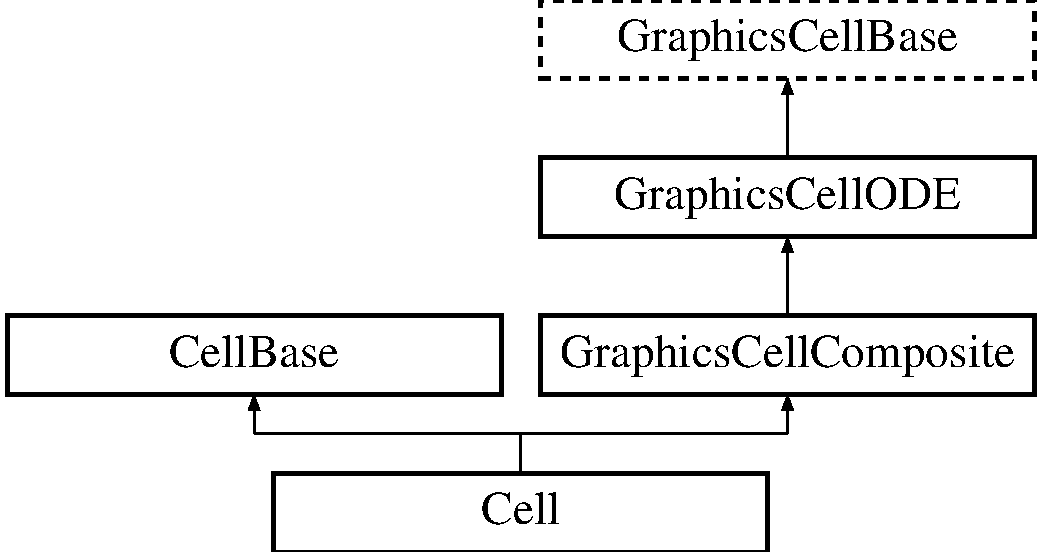
\includegraphics[height=4.000000cm]{class_cell}
\end{center}
\end{figure}
\subsection*{\-Public \-Member \-Functions}
\begin{DoxyCompactItemize}
\item 
\hyperlink{class_cell_a394510643e8664cf12b5efaf5cb99f71}{\-Cell} ()
\item 
virtual \hyperlink{class_cell_a9fa559f7a28e2b4336c6879ca09304d8}{$\sim$\-Cell} ()
\item 
\hyperlink{class_cell_aa0fda2bd78b5e4620e237cb7415bb62a}{\-Cell} (const \hyperlink{class_cell}{\-Cell} \&c2)
\item 
void \hyperlink{class_cell_a1762ba87b6cd232fb4d5ca9513600214}{initialize} (\-Cell\-Init\-Param \&p)
\item 
\hyperlink{class_cell}{\-Cell} \& \hyperlink{class_cell_a30910c960819ab01b80c4268a22b1579}{operator=} (const \hyperlink{class_cell}{\-Cell} \&c2)
\item 
double \hyperlink{class_cell_a4f4950f9901d2e52218da8421d11a78f}{get\-Time\-Dependent\-Volume} (const double time) const 
\item 
int \hyperlink{class_cell_a98b05ad9c5ba1a0bb719df105eb1b56f}{get\-N\-Channels} () const 
\item 
\-Array$<$ double, 1 $>$ \& \hyperlink{class_cell_abed1503a45db1ec72fe2f9721bb8dd7d}{get\-Propensities} ()
\item 
\-Array$<$ double, 1 $>$ \& \hyperlink{class_cell_a001e74a518b87008ab0235095b802677}{get\-Propensities\-Cell} ()
\item 
\-Array$<$ double, 1 $>$ \& \hyperlink{class_cell_aa277030af60d6cf9b0698e49a907996e}{get\-Propensities\-Cell\-Milieu} ()
\item 
double \hyperlink{class_cell_aaf492522ce24129fcac85bafb5dcc8f2}{get\-Angle} () const 
\item 
bool \hyperlink{class_cell_a15cfab0157a0180d1f409ed8afc5c14b}{is\-Reaction\-Internal} (int mu) const 
\item 
void \hyperlink{class_cell_a1eb2a609160163f5768e5708cd55a8e2}{set\-Reference\-Propensities} (\-Array$<$ double, 1 $>$ ref\-Array)
\item 
void \hyperlink{class_cell_a0559f4ae5b505afcd98a04ab259bc489}{apply\-Reaction} (int mu)
\item 
void \hyperlink{class_cell_ad872f4f01c39feb953ee27a9d37963af}{compute\-Propensities} ()
\item 
void \hyperlink{class_cell_a91e4b4765817d5287c69d21ff70906c9}{compute\-Propensities} (double time)
\item 
void \hyperlink{class_cell_ada072ae0aa05f43fda6daa196c8342d3}{compute\-Propensities\-Cell} ()
\item 
void \hyperlink{class_cell_a3502b355df87e09a247e4387b6dd4217}{compute\-Propensities\-Cell} (const double time)
\item 
void \hyperlink{class_cell_a8c5abd4f4386f83a8d3fc02ece00a5ef}{compute\-Propensities\-Cell\-Milieu} ()
\item 
void \hyperlink{class_cell_a0fe39496c6ca627b2930ce5923b3cb1c}{compute\-Propensities\-Cell\-Milieu} (const double time)
\item 
\hyperlink{class_cell}{\-Cell} \hyperlink{class_cell_a23acbe45a58bbed665c46528ec0717cd}{duplicate} ()
\item 
void \hyperlink{class_cell_a8fa3d31ea4774884a1dd0ce488f14123}{set\-Cell\-Index} (int i)
\item 
void \hyperlink{class_cell_a91d52e997836d430d05e5c810f553ce9}{set\-Angle} (double angle)
\item 
virtual void \hyperlink{class_cell_a7546388567cca19b27af68236161e91b}{set\-Position} (\-Tiny\-Vector$<$ double, 3 $>$ position)
\item 
void \hyperlink{class_cell_afea44081620717505850e33262a70472}{update\-Graphics\-Cell} (const double time)
\end{DoxyCompactItemize}
\subsection*{\-Static \-Public \-Member \-Functions}
\begin{DoxyCompactItemize}
\item 
static int \hyperlink{class_cell_ae2dfe08ecb85bc573d847bc992380e4a}{get\-N\-Cell\-Objects} ()
\end{DoxyCompactItemize}
\subsection*{\-Friends}
\begin{DoxyCompactItemize}
\item 
ostream \& \hyperlink{class_cell_ab7519ad9f97e822bc4c886ea1e85c29f}{operator$<$$<$} (ostream \&out, const \hyperlink{class_cell}{\-Cell} \&c)
\end{DoxyCompactItemize}


\subsection{\-Detailed \-Description}
\-Cell able to divide and communicate with the milieu.

\-This class is derived from \hyperlink{class_cell_base}{\-Cell\-Base} and defines the cells able to live in a milieu and divide.

\-Remark\-: it has a propensities array of size n\-Total\-Channels that contains the propensities of intracellular reactions and cell-\/milieu reactions. 

\-Definition at line 56 of file \-Cell.\-h.



\subsection{\-Constructor \& \-Destructor \-Documentation}
\hypertarget{class_cell_a394510643e8664cf12b5efaf5cb99f71}{\index{\-Cell@{\-Cell}!\-Cell@{\-Cell}}
\index{\-Cell@{\-Cell}!Cell@{\-Cell}}
\subsubsection[{\-Cell}]{\setlength{\rightskip}{0pt plus 5cm}{\bf \-Cell\-::\-Cell} (
\begin{DoxyParamCaption}
{}
\end{DoxyParamCaption}
)}}\label{class_cell_a394510643e8664cf12b5efaf5cb99f71}


\-Definition at line 30 of file \-Cell.\-cpp.

\hypertarget{class_cell_a9fa559f7a28e2b4336c6879ca09304d8}{\index{\-Cell@{\-Cell}!$\sim$\-Cell@{$\sim$\-Cell}}
\index{$\sim$\-Cell@{$\sim$\-Cell}!Cell@{\-Cell}}
\subsubsection[{$\sim$\-Cell}]{\setlength{\rightskip}{0pt plus 5cm}{\bf \-Cell\-::$\sim$\-Cell} (
\begin{DoxyParamCaption}
{}
\end{DoxyParamCaption}
)\hspace{0.3cm}{\ttfamily  \mbox{[}virtual\mbox{]}}}}\label{class_cell_a9fa559f7a28e2b4336c6879ca09304d8}


\-Definition at line 43 of file \-Cell.\-cpp.

\hypertarget{class_cell_aa0fda2bd78b5e4620e237cb7415bb62a}{\index{\-Cell@{\-Cell}!\-Cell@{\-Cell}}
\index{\-Cell@{\-Cell}!Cell@{\-Cell}}
\subsubsection[{\-Cell}]{\setlength{\rightskip}{0pt plus 5cm}{\bf \-Cell\-::\-Cell} (
\begin{DoxyParamCaption}
\item[{const {\bf \-Cell} \&}]{c2}
\end{DoxyParamCaption}
)}}\label{class_cell_aa0fda2bd78b5e4620e237cb7415bb62a}
\-Copy constructor. \-We need the copy constructor in order to use a \-Blitz++ array of \hyperlink{class_cell}{\-Cell} objects (unkown details of the implementation of the \-Blitz++ library). \-It is also used in the \hyperlink{class_cell_a23acbe45a58bbed665c46528ec0717cd}{duplicate()} method to return by value a copy of a \hyperlink{class_cell}{\-Cell} object. 

\-Definition at line 145 of file \-Cell.\-cpp.



\subsection{\-Member \-Function \-Documentation}
\hypertarget{class_cell_a0559f4ae5b505afcd98a04ab259bc489}{\index{\-Cell@{\-Cell}!apply\-Reaction@{apply\-Reaction}}
\index{apply\-Reaction@{apply\-Reaction}!Cell@{\-Cell}}
\subsubsection[{apply\-Reaction}]{\setlength{\rightskip}{0pt plus 5cm}void {\bf \-Cell\-::apply\-Reaction} (
\begin{DoxyParamCaption}
\item[{int}]{mu}
\end{DoxyParamCaption}
)}}\label{class_cell_a0559f4ae5b505afcd98a04ab259bc489}
\-Apply the reaction given by the channel number. \-Change the state of the cell based on the stoichiometric matrix. \-There are two cases depending on the channel number\-: it can concern an internal reaction (\hyperlink{class_cell_base_ae24860242d26c1eff241af04daaf06a0}{\-Cell\-Base\-::apply\-Reaction()}) or a cell-\/milieu reaction (cell\-Milieu\-Chemical\-System\-\_\-.\-apply\-Reaction()). 
\begin{DoxyParams}{\-Parameters}
{\em mu} & \mbox{[}in\mbox{]} channel number. \\
\hline
\end{DoxyParams}


\-Reimplemented from \hyperlink{class_cell_base_ae24860242d26c1eff241af04daaf06a0}{\-Cell\-Base}.



\-Definition at line 249 of file \-Cell.\-cpp.

\hypertarget{class_cell_ad872f4f01c39feb953ee27a9d37963af}{\index{\-Cell@{\-Cell}!compute\-Propensities@{compute\-Propensities}}
\index{compute\-Propensities@{compute\-Propensities}!Cell@{\-Cell}}
\subsubsection[{compute\-Propensities}]{\setlength{\rightskip}{0pt plus 5cm}void {\bf \-Cell\-::compute\-Propensities} (
\begin{DoxyParamCaption}
{}
\end{DoxyParamCaption}
)}}\label{class_cell_ad872f4f01c39feb953ee27a9d37963af}
\-Compute the propensities of all reaction channels, including the internal and cell-\/milieu reactions. 

\-Reimplemented from \hyperlink{class_cell_base_a36d16b84e0291e317fcf2425bbd6a953}{\-Cell\-Base}.



\-Definition at line 270 of file \-Cell.\-cpp.

\hypertarget{class_cell_a91e4b4765817d5287c69d21ff70906c9}{\index{\-Cell@{\-Cell}!compute\-Propensities@{compute\-Propensities}}
\index{compute\-Propensities@{compute\-Propensities}!Cell@{\-Cell}}
\subsubsection[{compute\-Propensities}]{\setlength{\rightskip}{0pt plus 5cm}void {\bf \-Cell\-::compute\-Propensities} (
\begin{DoxyParamCaption}
\item[{double}]{time}
\end{DoxyParamCaption}
)}}\label{class_cell_a91e4b4765817d5287c69d21ff70906c9}
\-Compute the propensities of all reaction channels, including the internal and cell-\/milieu reactions, some of them having time-\/dependent reaction rates. 

\-Reimplemented from \hyperlink{class_cell_base_a17dcaf6ab4ce71d41640de772822ea79}{\-Cell\-Base}.



\-Definition at line 278 of file \-Cell.\-cpp.

\hypertarget{class_cell_ada072ae0aa05f43fda6daa196c8342d3}{\index{\-Cell@{\-Cell}!compute\-Propensities\-Cell@{compute\-Propensities\-Cell}}
\index{compute\-Propensities\-Cell@{compute\-Propensities\-Cell}!Cell@{\-Cell}}
\subsubsection[{compute\-Propensities\-Cell}]{\setlength{\rightskip}{0pt plus 5cm}void {\bf \-Cell\-::compute\-Propensities\-Cell} (
\begin{DoxyParamCaption}
{}
\end{DoxyParamCaption}
)}}\label{class_cell_ada072ae0aa05f43fda6daa196c8342d3}
\-Compute the propensities {\bfseries only} of the intracellular reaction channels. 

\-Definition at line 292 of file \-Cell.\-cpp.

\hypertarget{class_cell_a3502b355df87e09a247e4387b6dd4217}{\index{\-Cell@{\-Cell}!compute\-Propensities\-Cell@{compute\-Propensities\-Cell}}
\index{compute\-Propensities\-Cell@{compute\-Propensities\-Cell}!Cell@{\-Cell}}
\subsubsection[{compute\-Propensities\-Cell}]{\setlength{\rightskip}{0pt plus 5cm}void {\bf \-Cell\-::compute\-Propensities\-Cell} (
\begin{DoxyParamCaption}
\item[{const double}]{time}
\end{DoxyParamCaption}
)}}\label{class_cell_a3502b355df87e09a247e4387b6dd4217}


\-Definition at line 299 of file \-Cell.\-cpp.

\hypertarget{class_cell_a8c5abd4f4386f83a8d3fc02ece00a5ef}{\index{\-Cell@{\-Cell}!compute\-Propensities\-Cell\-Milieu@{compute\-Propensities\-Cell\-Milieu}}
\index{compute\-Propensities\-Cell\-Milieu@{compute\-Propensities\-Cell\-Milieu}!Cell@{\-Cell}}
\subsubsection[{compute\-Propensities\-Cell\-Milieu}]{\setlength{\rightskip}{0pt plus 5cm}void {\bf \-Cell\-::compute\-Propensities\-Cell\-Milieu} (
\begin{DoxyParamCaption}
{}
\end{DoxyParamCaption}
)}}\label{class_cell_a8c5abd4f4386f83a8d3fc02ece00a5ef}
\-Compute the propensities {\bfseries only} of the cell-\/milieu reaction channels. 

\-Definition at line 306 of file \-Cell.\-cpp.

\hypertarget{class_cell_a0fe39496c6ca627b2930ce5923b3cb1c}{\index{\-Cell@{\-Cell}!compute\-Propensities\-Cell\-Milieu@{compute\-Propensities\-Cell\-Milieu}}
\index{compute\-Propensities\-Cell\-Milieu@{compute\-Propensities\-Cell\-Milieu}!Cell@{\-Cell}}
\subsubsection[{compute\-Propensities\-Cell\-Milieu}]{\setlength{\rightskip}{0pt plus 5cm}void {\bf \-Cell\-::compute\-Propensities\-Cell\-Milieu} (
\begin{DoxyParamCaption}
\item[{const double}]{time}
\end{DoxyParamCaption}
)}}\label{class_cell_a0fe39496c6ca627b2930ce5923b3cb1c}


\-Definition at line 313 of file \-Cell.\-cpp.

\hypertarget{class_cell_a23acbe45a58bbed665c46528ec0717cd}{\index{\-Cell@{\-Cell}!duplicate@{duplicate}}
\index{duplicate@{duplicate}!Cell@{\-Cell}}
\subsubsection[{duplicate}]{\setlength{\rightskip}{0pt plus 5cm}{\bf \-Cell} {\bf \-Cell\-::duplicate} (
\begin{DoxyParamCaption}
{}
\end{DoxyParamCaption}
)}}\label{class_cell_a23acbe45a58bbed665c46528ec0717cd}
\-Duplicate the cell and returns by value the daughter cell.
\begin{DoxyItemize}
\item \-Detach proteins from \-D\-N\-A.
\item \-Make a copy of the cell.
\item \-Distribute proteins between the two cells.
\item \-Set the time of next division for both cells.
\item \-Return by value the new daughter cell (needs \hyperlink{class_cell}{\-Cell} copy constructor). 
\end{DoxyItemize}

\-Definition at line 348 of file \-Cell.\-cpp.

\hypertarget{class_cell_aaf492522ce24129fcac85bafb5dcc8f2}{\index{\-Cell@{\-Cell}!get\-Angle@{get\-Angle}}
\index{get\-Angle@{get\-Angle}!Cell@{\-Cell}}
\subsubsection[{get\-Angle}]{\setlength{\rightskip}{0pt plus 5cm}double {\bf \-Cell\-::get\-Angle} (
\begin{DoxyParamCaption}
{}
\end{DoxyParamCaption}
) const}}\label{class_cell_aaf492522ce24129fcac85bafb5dcc8f2}


\-Reimplemented from \hyperlink{class_cell_base_a3fb7f0f49934e83a0ed1cd2d82fba99e}{\-Cell\-Base}.



\-Definition at line 228 of file \-Cell.\-cpp.

\hypertarget{class_cell_ae2dfe08ecb85bc573d847bc992380e4a}{\index{\-Cell@{\-Cell}!get\-N\-Cell\-Objects@{get\-N\-Cell\-Objects}}
\index{get\-N\-Cell\-Objects@{get\-N\-Cell\-Objects}!Cell@{\-Cell}}
\subsubsection[{get\-N\-Cell\-Objects}]{\setlength{\rightskip}{0pt plus 5cm}static int {\bf \-Cell\-::get\-N\-Cell\-Objects} (
\begin{DoxyParamCaption}
{}
\end{DoxyParamCaption}
)\hspace{0.3cm}{\ttfamily  \mbox{[}inline, static\mbox{]}}}}\label{class_cell_ae2dfe08ecb85bc573d847bc992380e4a}
\-Get the total number of \hyperlink{class_cell}{\-Cell} objects. 

\-Definition at line 110 of file \-Cell.\-h.

\hypertarget{class_cell_a98b05ad9c5ba1a0bb719df105eb1b56f}{\index{\-Cell@{\-Cell}!get\-N\-Channels@{get\-N\-Channels}}
\index{get\-N\-Channels@{get\-N\-Channels}!Cell@{\-Cell}}
\subsubsection[{get\-N\-Channels}]{\setlength{\rightskip}{0pt plus 5cm}int {\bf \-Cell\-::get\-N\-Channels} (
\begin{DoxyParamCaption}
{}
\end{DoxyParamCaption}
) const\hspace{0.3cm}{\ttfamily  \mbox{[}inline\mbox{]}}}}\label{class_cell_a98b05ad9c5ba1a0bb719df105eb1b56f}
\-Returns the total number of channels (internal + cell-\/milieu). 

\-Reimplemented from \hyperlink{class_cell_base_ac63ef2dae0215b9fb430dcc40378f2ce}{\-Cell\-Base}.



\-Definition at line 313 of file \-Cell.\-h.

\hypertarget{class_cell_abed1503a45db1ec72fe2f9721bb8dd7d}{\index{\-Cell@{\-Cell}!get\-Propensities@{get\-Propensities}}
\index{get\-Propensities@{get\-Propensities}!Cell@{\-Cell}}
\subsubsection[{get\-Propensities}]{\setlength{\rightskip}{0pt plus 5cm}\-Array$<$ double, 1 $>$ \& {\bf \-Cell\-::get\-Propensities} (
\begin{DoxyParamCaption}
{}
\end{DoxyParamCaption}
)\hspace{0.3cm}{\ttfamily  \mbox{[}inline\mbox{]}}}}\label{class_cell_abed1503a45db1ec72fe2f9721bb8dd7d}
\-Returns the total array of propensities (internal + cell-\/milieu). 

\-Reimplemented from \hyperlink{class_cell_base_ad176550eea24417e8972346acb4c0640}{\-Cell\-Base}.



\-Definition at line 316 of file \-Cell.\-h.

\hypertarget{class_cell_a001e74a518b87008ab0235095b802677}{\index{\-Cell@{\-Cell}!get\-Propensities\-Cell@{get\-Propensities\-Cell}}
\index{get\-Propensities\-Cell@{get\-Propensities\-Cell}!Cell@{\-Cell}}
\subsubsection[{get\-Propensities\-Cell}]{\setlength{\rightskip}{0pt plus 5cm}\-Array$<$ double, 1 $>$ \& {\bf \-Cell\-::get\-Propensities\-Cell} (
\begin{DoxyParamCaption}
{}
\end{DoxyParamCaption}
)\hspace{0.3cm}{\ttfamily  \mbox{[}inline\mbox{]}}}}\label{class_cell_a001e74a518b87008ab0235095b802677}
\-Returns the array of propensities of the cell reactions. 

\-Definition at line 319 of file \-Cell.\-h.

\hypertarget{class_cell_aa277030af60d6cf9b0698e49a907996e}{\index{\-Cell@{\-Cell}!get\-Propensities\-Cell\-Milieu@{get\-Propensities\-Cell\-Milieu}}
\index{get\-Propensities\-Cell\-Milieu@{get\-Propensities\-Cell\-Milieu}!Cell@{\-Cell}}
\subsubsection[{get\-Propensities\-Cell\-Milieu}]{\setlength{\rightskip}{0pt plus 5cm}\-Array$<$ double, 1 $>$ \& {\bf \-Cell\-::get\-Propensities\-Cell\-Milieu} (
\begin{DoxyParamCaption}
{}
\end{DoxyParamCaption}
)\hspace{0.3cm}{\ttfamily  \mbox{[}inline\mbox{]}}}}\label{class_cell_aa277030af60d6cf9b0698e49a907996e}
\-Returns the array of propensities of the cell-\/milieu reactions. 

\-Definition at line 322 of file \-Cell.\-h.

\hypertarget{class_cell_a4f4950f9901d2e52218da8421d11a78f}{\index{\-Cell@{\-Cell}!get\-Time\-Dependent\-Volume@{get\-Time\-Dependent\-Volume}}
\index{get\-Time\-Dependent\-Volume@{get\-Time\-Dependent\-Volume}!Cell@{\-Cell}}
\subsubsection[{get\-Time\-Dependent\-Volume}]{\setlength{\rightskip}{0pt plus 5cm}double {\bf \-Cell\-::get\-Time\-Dependent\-Volume} (
\begin{DoxyParamCaption}
\item[{const double}]{time}
\end{DoxyParamCaption}
) const\hspace{0.3cm}{\ttfamily  \mbox{[}virtual\mbox{]}}}}\label{class_cell_a4f4950f9901d2e52218da8421d11a78f}


\-Implements \hyperlink{class_cell_base_a7b69eec41c172b719e7f2ea6cb277ce9}{\-Cell\-Base}.



\-Definition at line 418 of file \-Cell.\-cpp.

\hypertarget{class_cell_a1762ba87b6cd232fb4d5ca9513600214}{\index{\-Cell@{\-Cell}!initialize@{initialize}}
\index{initialize@{initialize}!Cell@{\-Cell}}
\subsubsection[{initialize}]{\setlength{\rightskip}{0pt plus 5cm}void {\bf \-Cell\-::initialize} (
\begin{DoxyParamCaption}
\item[{\-Cell\-Init\-Param \&}]{p}
\end{DoxyParamCaption}
)}}\label{class_cell_a1762ba87b6cd232fb4d5ca9513600214}
\-Initialize and define a \hyperlink{class_cell}{\-Cell} object, including dna\-Species array and cell-\/milieu reactions.

\-The propensities array will have the size n\-Channels + n\-Channels\-Milieu. \-The propensities array for internal reactions (from \hyperlink{class_cell_base}{\-Cell\-Base} class) is referenced to the subarray \#total\-Propensities\-\_\-(0,n\-Channels-\/1) and the prop. array for cell-\/milieu reactions is referenced to the subarray \#total\-Propensities\-\_\-(n\-Channels,n\-Total\-Channels). 

\-Definition at line 52 of file \-Cell.\-cpp.

\hypertarget{class_cell_a15cfab0157a0180d1f409ed8afc5c14b}{\index{\-Cell@{\-Cell}!is\-Reaction\-Internal@{is\-Reaction\-Internal}}
\index{is\-Reaction\-Internal@{is\-Reaction\-Internal}!Cell@{\-Cell}}
\subsubsection[{is\-Reaction\-Internal}]{\setlength{\rightskip}{0pt plus 5cm}bool {\bf \-Cell\-::is\-Reaction\-Internal} (
\begin{DoxyParamCaption}
\item[{int}]{mu}
\end{DoxyParamCaption}
) const\hspace{0.3cm}{\ttfamily  \mbox{[}inline\mbox{]}}}}\label{class_cell_a15cfab0157a0180d1f409ed8afc5c14b}


\-Definition at line 325 of file \-Cell.\-h.

\hypertarget{class_cell_a30910c960819ab01b80c4268a22b1579}{\index{\-Cell@{\-Cell}!operator=@{operator=}}
\index{operator=@{operator=}!Cell@{\-Cell}}
\subsubsection[{operator=}]{\setlength{\rightskip}{0pt plus 5cm}{\bf \-Cell} \& \-Cell\-::operator= (
\begin{DoxyParamCaption}
\item[{const {\bf \-Cell} \&}]{c2}
\end{DoxyParamCaption}
)}}\label{class_cell_a30910c960819ab01b80c4268a22b1579}
\-Assignment operator. 

\-Definition at line 160 of file \-Cell.\-cpp.

\hypertarget{class_cell_a91d52e997836d430d05e5c810f553ce9}{\index{\-Cell@{\-Cell}!set\-Angle@{set\-Angle}}
\index{set\-Angle@{set\-Angle}!Cell@{\-Cell}}
\subsubsection[{set\-Angle}]{\setlength{\rightskip}{0pt plus 5cm}void {\bf \-Cell\-::set\-Angle} (
\begin{DoxyParamCaption}
\item[{double}]{angle}
\end{DoxyParamCaption}
)}}\label{class_cell_a91d52e997836d430d05e5c810f553ce9}
\-Change the angle of the cell. 

\-Reimplemented from \hyperlink{class_cell_base_a8ab82721972f41f1d233ab17a841580c}{\-Cell\-Base}.



\-Definition at line 220 of file \-Cell.\-cpp.

\hypertarget{class_cell_a8fa3d31ea4774884a1dd0ce488f14123}{\index{\-Cell@{\-Cell}!set\-Cell\-Index@{set\-Cell\-Index}}
\index{set\-Cell\-Index@{set\-Cell\-Index}!Cell@{\-Cell}}
\subsubsection[{set\-Cell\-Index}]{\setlength{\rightskip}{0pt plus 5cm}void {\bf \-Cell\-::set\-Cell\-Index} (
\begin{DoxyParamCaption}
\item[{int}]{i}
\end{DoxyParamCaption}
)}}\label{class_cell_a8fa3d31ea4774884a1dd0ce488f14123}
\-Set the cell index in the \hyperlink{class_graphics_cell_composite}{\-Graphics\-Cell\-Composite} class. \-The cell index should be directly used in the \hyperlink{class_cell}{\-Cell} class, it is just used by the graphical interface to know which cell it is when interacting with it. 

\-Reimplemented from \hyperlink{class_graphics_cell_base_a1bd5925a454cd3926652de53ce584f68}{\-Graphics\-Cell\-Base}.



\-Definition at line 189 of file \-Cell.\-cpp.

\hypertarget{class_cell_a7546388567cca19b27af68236161e91b}{\index{\-Cell@{\-Cell}!set\-Position@{set\-Position}}
\index{set\-Position@{set\-Position}!Cell@{\-Cell}}
\subsubsection[{set\-Position}]{\setlength{\rightskip}{0pt plus 5cm}void {\bf \-Cell\-::set\-Position} (
\begin{DoxyParamCaption}
\item[{\-Tiny\-Vector$<$ double, 3 $>$}]{position}
\end{DoxyParamCaption}
)\hspace{0.3cm}{\ttfamily  \mbox{[}virtual\mbox{]}}}}\label{class_cell_a7546388567cca19b27af68236161e91b}
\-Set the position of the cell, both in \hyperlink{class_cell_base}{\-Cell\-Base} and \hyperlink{class_graphics_cell_composite}{\-Graphics\-Cell\-Composite} classes. 

\-Reimplemented from \hyperlink{class_cell_base_a913046f5a53f8960f5c17252df6056df}{\-Cell\-Base}.



\-Definition at line 212 of file \-Cell.\-cpp.

\hypertarget{class_cell_a1eb2a609160163f5768e5708cd55a8e2}{\index{\-Cell@{\-Cell}!set\-Reference\-Propensities@{set\-Reference\-Propensities}}
\index{set\-Reference\-Propensities@{set\-Reference\-Propensities}!Cell@{\-Cell}}
\subsubsection[{set\-Reference\-Propensities}]{\setlength{\rightskip}{0pt plus 5cm}void {\bf \-Cell\-::set\-Reference\-Propensities} (
\begin{DoxyParamCaption}
\item[{\-Array$<$ double, 1 $>$}]{ref\-Array}
\end{DoxyParamCaption}
)}}\label{class_cell_a1eb2a609160163f5768e5708cd55a8e2}
\-Set the propensities array to be a reference to another array. \-This method set the \#total\-Propensities\-\_\- array to be a reference to another array and it also set the reference of the sub arrays in the \hyperlink{class_cell_base}{\-Cell\-Base} class \-Cell\-Base\-::state\-\_\-.\-propensities\-\_\- and in the \hyperlink{class_cell_milieu_chemical_system}{\-Cell\-Milieu\-Chemical\-System} class \#cell\-Milieu\-Chemical\-System\-\_\-.\-propensities\-\_\- . 

\-Reimplemented from \hyperlink{class_cell_base_afd447b811d2bacc971aba82447a8123e}{\-Cell\-Base}.



\-Definition at line 196 of file \-Cell.\-cpp.

\hypertarget{class_cell_afea44081620717505850e33262a70472}{\index{\-Cell@{\-Cell}!update\-Graphics\-Cell@{update\-Graphics\-Cell}}
\index{update\-Graphics\-Cell@{update\-Graphics\-Cell}!Cell@{\-Cell}}
\subsubsection[{update\-Graphics\-Cell}]{\setlength{\rightskip}{0pt plus 5cm}void {\bf \-Cell\-::update\-Graphics\-Cell} (
\begin{DoxyParamCaption}
\item[{const double}]{time}
\end{DoxyParamCaption}
)}}\label{class_cell_afea44081620717505850e33262a70472}
\-Copy the cell dimensions and position from the \hyperlink{class_cell_base_a966e4298cabc00986bb03ce92dfad1f5}{\-Cell\-Base\-::state\-\_\-} to the \hyperlink{class_graphics_cell_composite}{\-Graphics\-Cell\-Composite} class. 

\-Definition at line 237 of file \-Cell.\-cpp.



\subsection{\-Friends \-And \-Related \-Function \-Documentation}
\hypertarget{class_cell_ab7519ad9f97e822bc4c886ea1e85c29f}{\index{\-Cell@{\-Cell}!operator$<$$<$@{operator$<$$<$}}
\index{operator$<$$<$@{operator$<$$<$}!Cell@{\-Cell}}
\subsubsection[{operator$<$$<$}]{\setlength{\rightskip}{0pt plus 5cm}ostream\& operator$<$$<$ (
\begin{DoxyParamCaption}
\item[{ostream \&}]{out, }
\item[{const {\bf \-Cell} \&}]{c}
\end{DoxyParamCaption}
)\hspace{0.3cm}{\ttfamily  \mbox{[}friend\mbox{]}}}}\label{class_cell_ab7519ad9f97e822bc4c886ea1e85c29f}
\-Operator that outputs the content of a \hyperlink{class_cell}{\-Cell} state. \-Remark\-: it is declared as a friend operator, so that it has access to the private part of the \hyperlink{class_cell}{\-Cell} class. \-Overloading the $<$$<$ operator of class \hyperlink{class_cell_base}{\-Cell\-Base}. 

\-Definition at line 176 of file \-Cell.\-cpp.



\-The documentation for this class was generated from the following files\-:\begin{DoxyCompactItemize}
\item 
/media/\-My\-Passport\-Blue/\-Data/\-Research/\-Simulations/\-Colony/\hyperlink{_cell_8h}{\-Cell.\-h}\item 
/media/\-My\-Passport\-Blue/\-Data/\-Research/\-Simulations/\-Colony/\hyperlink{_cell_8cpp}{\-Cell.\-cpp}\end{DoxyCompactItemize}

\hypertarget{class_cell_base}{\section{\-Cell\-Base \-Class \-Reference}
\label{class_cell_base}\index{\-Cell\-Base@{\-Cell\-Base}}
}


{\ttfamily \#include $<$\-Cell\-Base.\-h$>$}

\-Inheritance diagram for \-Cell\-Base\-:\begin{figure}[H]
\begin{center}
\leavevmode
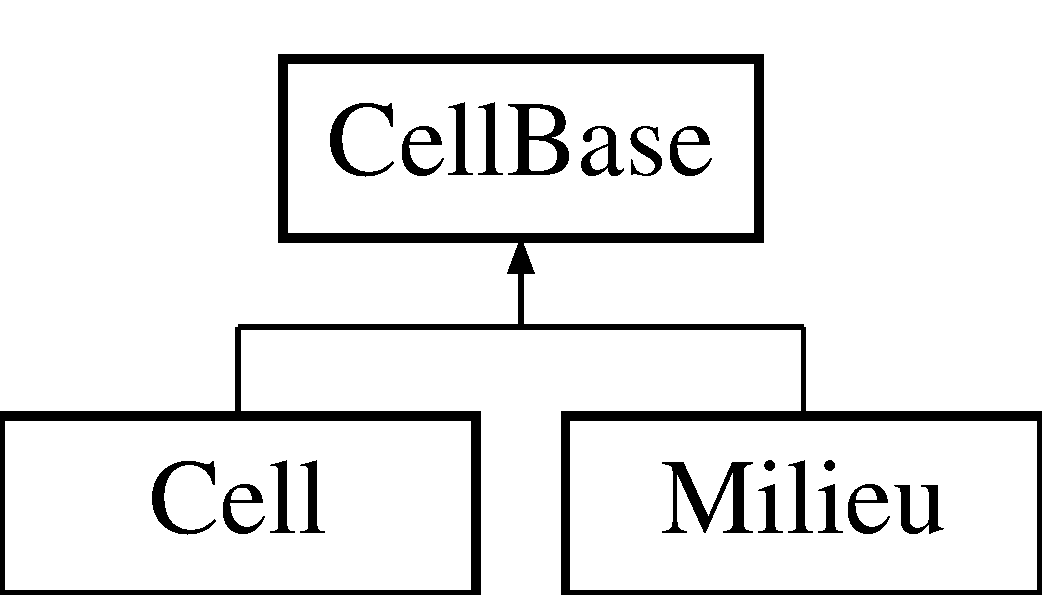
\includegraphics[height=2.000000cm]{class_cell_base}
\end{center}
\end{figure}
\subsection*{\-Public \-Member \-Functions}
\begin{DoxyCompactItemize}
\item 
virtual \hyperlink{class_cell_base_a91df7ce6090723939914fc08ae5dd25e}{$\sim$\-Cell\-Base} ()
\item 
void \hyperlink{class_cell_base_a442489e1986f767c2a0530c01a134057}{initialize} (\-Cell\-Base\-Init\-Param \&p)
\item 
int \hyperlink{class_cell_base_ac63ef2dae0215b9fb430dcc40378f2ce}{get\-N\-Channels} () const 
\item 
int \hyperlink{class_cell_base_a870a19609d2b3910a4893be9d29799be}{get\-N\-Species} () const 
\item 
double \hyperlink{class_cell_base_a4ef31e07bbd457ce98bd354ffca1154e}{get\-Volume0} () const 
\item 
double \hyperlink{class_cell_base_a359d654fd26a50c59ad8eb37bdd3d0fd}{get\-Cell\-Length0} () const 
\item 
double \hyperlink{class_cell_base_a2c2d7a9f7729aff66186a69682c537b6}{get\-Cell\-Height0} () const 
\item 
virtual double \hyperlink{class_cell_base_a7b69eec41c172b719e7f2ea6cb277ce9}{get\-Time\-Dependent\-Volume} (const double time) const =0
\item 
\-Tiny\-Vector$<$ double, 3 $>$ \hyperlink{class_cell_base_a9776bb276fe4c6dc00448e5c9c6f4486}{get\-Time\-Dependent\-Cell\-Dimensions} (const double time)
\item 
\-Array$<$ int, 1 $>$ \& \hyperlink{class_cell_base_a72403c587aa2e64ba662a1f0c5ad5283}{get\-X} ()
\item 
\-Array$<$ double, 1 $>$ \& \hyperlink{class_cell_base_a12d1351b10bdacb89963176f5a576354}{get\-X\-Conc} ()
\item 
\-Array$<$ double, 1 $>$ \hyperlink{class_cell_base_a1e0fbdf9180c81c682b318d0f280ae3b}{get\-Xconc} (const double time) const 
\item 
\-Array$<$ double, 1 $>$ \& \hyperlink{class_cell_base_ad176550eea24417e8972346acb4c0640}{get\-Propensities} ()
\item 
double \hyperlink{class_cell_base_a9fe443b9b862fdafde0c05bb47b34c0a}{get\-Time\-Next\-Division} () const 
\item 
double \hyperlink{class_cell_base_a9e8640e5d32e13570bb41ef527bb66de}{get\-Time\-Previous\-Division} () const 
\item 
double \hyperlink{class_cell_base_aebfee0ab9fcf545450f015019ed228ce}{get\-Cell\-Cycle\-Duration} () const 
\item 
double \hyperlink{class_cell_base_aa37b1fc8ce2ca9cea42d647e7b320508}{get\-Cell\-Cycle\-Phase} (double time) const 
\item 
double \hyperlink{class_cell_base_a3fb7f0f49934e83a0ed1cd2d82fba99e}{get\-Angle} () const 
\item 
\-Tiny\-Vector$<$ double, 3 $>$ \hyperlink{class_cell_base_a32874d1193fa5b7a7fe7ccc3c1cfda98}{get\-Position} () const 
\item 
vector$<$ string $>$ \hyperlink{class_cell_base_ae8abd7753ef0e29bc858a35574554085}{get\-List\-Species\-Name} () const 
\item 
void \hyperlink{class_cell_base_ad67a9e2a335b88e788a6fb59fb1ee93a}{change\-Volume0\-By} (double volume0\-Change)
\item 
void \hyperlink{class_cell_base_ae24860242d26c1eff241af04daaf06a0}{apply\-Reaction} (int mu)
\item 
void \hyperlink{class_cell_base_a64655783b5cffb637ae4dd41403942e3}{apply\-Inter\-Cellular\-Reaction} (\-Array$<$ int, 1 $>$ stoich\-Vector)
\item 
void \hyperlink{class_cell_base_a36d16b84e0291e317fcf2425bbd6a953}{compute\-Propensities} ()
\item 
void \hyperlink{class_cell_base_a17dcaf6ab4ce71d41640de772822ea79}{compute\-Propensities} (const double time)
\item 
void \hyperlink{class_cell_base_a00a0fa8efa67c71ca357458f7f29a8c8}{compute\-Propensities\-Time\-Dependent\-Reactions} (const double time)
\item 
void \hyperlink{class_cell_base_aee22c1932b129c07afaf7f6ecac79d9b}{set\-Reference\-X} (\-Array$<$ int, 1 $>$ \&ref\-Array)
\item 
void \hyperlink{class_cell_base_a3337e4c5aa43f7fe166dc19df4142510}{set\-Reference\-X\-Conc} (\-Array$<$ double, 1 $>$ \&ref\-Array)
\item 
void \hyperlink{class_cell_base_afd447b811d2bacc971aba82447a8123e}{set\-Reference\-Propensities} (\-Array$<$ double, 1 $>$ ref\-Array)
\item 
void \hyperlink{class_cell_base_a3d2b95cda02a4fd4b2b33dd38e1e9817}{check\-Positivity} () const 
\item 
void \hyperlink{class_cell_base_a8ab82721972f41f1d233ab17a841580c}{set\-Angle} (double angle)
\item 
virtual void \hyperlink{class_cell_base_a913046f5a53f8960f5c17252df6056df}{set\-Position} (\-Tiny\-Vector$<$ double, 3 $>$ position)
\end{DoxyCompactItemize}
\subsection*{\-Protected \-Member \-Functions}
\begin{DoxyCompactItemize}
\item 
\hyperlink{class_cell_base_ac5cbc18d3f767bb91d9e052a3eb778b5}{\-Cell\-Base} ()
\item 
void \hyperlink{class_cell_base_a614fb1ef7fdd9ff936bfb941736a2fb8}{copy} (const \hyperlink{class_cell_base}{\-Cell\-Base} \&c2)
\end{DoxyCompactItemize}
\subsection*{\-Protected \-Attributes}
\begin{DoxyCompactItemize}
\item 
\hyperlink{class_state}{\-State} \hyperlink{class_cell_base_a966e4298cabc00986bb03ce92dfad1f5}{state\-\_\-}
\item 
\hyperlink{class_chemical_system}{\-Chemical\-System} \hyperlink{class_cell_base_ad40c4890431f5857c449a6470f80d15c}{chemical\-System\-\_\-}
\end{DoxyCompactItemize}
\subsection*{\-Friends}
\begin{DoxyCompactItemize}
\item 
ostream \& \hyperlink{class_cell_base_ad3061d9b136ee7884ff7c255a977fd78}{operator$<$$<$} (ostream \&out, const \hyperlink{class_cell_base}{\-Cell\-Base} \&c)
\end{DoxyCompactItemize}


\subsection{\-Detailed \-Description}
\-Base class for cell.

\-This class defines the basic \hyperlink{class_cell}{\-Cell} objects. \-They contains an internal state and a chemical system, as well as methods to compute the propensities and apply a reaction. 

\-Definition at line 56 of file \-Cell\-Base.\-h.



\subsection{\-Constructor \& \-Destructor \-Documentation}
\hypertarget{class_cell_base_ac5cbc18d3f767bb91d9e052a3eb778b5}{\index{\-Cell\-Base@{\-Cell\-Base}!\-Cell\-Base@{\-Cell\-Base}}
\index{\-Cell\-Base@{\-Cell\-Base}!CellBase@{\-Cell\-Base}}
\subsubsection[{\-Cell\-Base}]{\setlength{\rightskip}{0pt plus 5cm}{\bf \-Cell\-Base\-::\-Cell\-Base} (
\begin{DoxyParamCaption}
{}
\end{DoxyParamCaption}
)\hspace{0.3cm}{\ttfamily  \mbox{[}protected\mbox{]}}}}\label{class_cell_base_ac5cbc18d3f767bb91d9e052a3eb778b5}
\-Default constructor is protected. \hyperlink{class_cell_base}{\-Cell\-Base} objects cannot be instantiated directly by the user. \-The protected access assures that only the subclasses can instanciate. 

\-Definition at line 20 of file \-Cell\-Base.\-cpp.

\hypertarget{class_cell_base_a91df7ce6090723939914fc08ae5dd25e}{\index{\-Cell\-Base@{\-Cell\-Base}!$\sim$\-Cell\-Base@{$\sim$\-Cell\-Base}}
\index{$\sim$\-Cell\-Base@{$\sim$\-Cell\-Base}!CellBase@{\-Cell\-Base}}
\subsubsection[{$\sim$\-Cell\-Base}]{\setlength{\rightskip}{0pt plus 5cm}{\bf \-Cell\-Base\-::$\sim$\-Cell\-Base} (
\begin{DoxyParamCaption}
{}
\end{DoxyParamCaption}
)\hspace{0.3cm}{\ttfamily  \mbox{[}virtual\mbox{]}}}}\label{class_cell_base_a91df7ce6090723939914fc08ae5dd25e}


\-Definition at line 25 of file \-Cell\-Base.\-cpp.



\subsection{\-Member \-Function \-Documentation}
\hypertarget{class_cell_base_a64655783b5cffb637ae4dd41403942e3}{\index{\-Cell\-Base@{\-Cell\-Base}!apply\-Inter\-Cellular\-Reaction@{apply\-Inter\-Cellular\-Reaction}}
\index{apply\-Inter\-Cellular\-Reaction@{apply\-Inter\-Cellular\-Reaction}!CellBase@{\-Cell\-Base}}
\subsubsection[{apply\-Inter\-Cellular\-Reaction}]{\setlength{\rightskip}{0pt plus 5cm}void {\bf \-Cell\-Base\-::apply\-Inter\-Cellular\-Reaction} (
\begin{DoxyParamCaption}
\item[{\-Array$<$ int, 1 $>$}]{stoich\-Vector}
\end{DoxyParamCaption}
)}}\label{class_cell_base_a64655783b5cffb637ae4dd41403942e3}
\-Apply a chemical reaction that is defined outside the \hyperlink{class_cell}{\-Cell} class. \-This function takes as input the stoich\-Vector of the reaction and apply it to the state of the cell. 

\-Definition at line 108 of file \-Cell\-Base.\-cpp.

\hypertarget{class_cell_base_ae24860242d26c1eff241af04daaf06a0}{\index{\-Cell\-Base@{\-Cell\-Base}!apply\-Reaction@{apply\-Reaction}}
\index{apply\-Reaction@{apply\-Reaction}!CellBase@{\-Cell\-Base}}
\subsubsection[{apply\-Reaction}]{\setlength{\rightskip}{0pt plus 5cm}void {\bf \-Cell\-Base\-::apply\-Reaction} (
\begin{DoxyParamCaption}
\item[{int}]{mu}
\end{DoxyParamCaption}
)}}\label{class_cell_base_ae24860242d26c1eff241af04daaf06a0}
\-Apply the reaction given by the channel number. \-Change the state of the cell based on the stoichiometric matrix. 

\-Reimplemented in \hyperlink{class_cell_a0559f4ae5b505afcd98a04ab259bc489}{\-Cell}.



\-Definition at line 92 of file \-Cell\-Base.\-cpp.

\hypertarget{class_cell_base_ad67a9e2a335b88e788a6fb59fb1ee93a}{\index{\-Cell\-Base@{\-Cell\-Base}!change\-Volume0\-By@{change\-Volume0\-By}}
\index{change\-Volume0\-By@{change\-Volume0\-By}!CellBase@{\-Cell\-Base}}
\subsubsection[{change\-Volume0\-By}]{\setlength{\rightskip}{0pt plus 5cm}void {\bf \-Cell\-Base\-::change\-Volume0\-By} (
\begin{DoxyParamCaption}
\item[{double}]{volume0\-Change}
\end{DoxyParamCaption}
)}}\label{class_cell_base_ad67a9e2a335b88e788a6fb59fb1ee93a}


\-Definition at line 85 of file \-Cell\-Base.\-cpp.

\hypertarget{class_cell_base_a3d2b95cda02a4fd4b2b33dd38e1e9817}{\index{\-Cell\-Base@{\-Cell\-Base}!check\-Positivity@{check\-Positivity}}
\index{check\-Positivity@{check\-Positivity}!CellBase@{\-Cell\-Base}}
\subsubsection[{check\-Positivity}]{\setlength{\rightskip}{0pt plus 5cm}void {\bf \-Cell\-Base\-::check\-Positivity} (
\begin{DoxyParamCaption}
{}
\end{DoxyParamCaption}
) const}}\label{class_cell_base_a3d2b95cda02a4fd4b2b33dd38e1e9817}
\-Check that the number of molecules in state vector x is positive. \hypertarget{class_cell_base_a36d16b84e0291e317fcf2425bbd6a953}{\index{\-Cell\-Base@{\-Cell\-Base}!compute\-Propensities@{compute\-Propensities}}
\index{compute\-Propensities@{compute\-Propensities}!CellBase@{\-Cell\-Base}}
\subsubsection[{compute\-Propensities}]{\setlength{\rightskip}{0pt plus 5cm}void {\bf \-Cell\-Base\-::compute\-Propensities} (
\begin{DoxyParamCaption}
{}
\end{DoxyParamCaption}
)}}\label{class_cell_base_a36d16b84e0291e317fcf2425bbd6a953}
\-Compute the propensities of all reaction channels. 

\-Reimplemented in \hyperlink{class_cell_ad872f4f01c39feb953ee27a9d37963af}{\-Cell}.



\-Definition at line 119 of file \-Cell\-Base.\-cpp.

\hypertarget{class_cell_base_a17dcaf6ab4ce71d41640de772822ea79}{\index{\-Cell\-Base@{\-Cell\-Base}!compute\-Propensities@{compute\-Propensities}}
\index{compute\-Propensities@{compute\-Propensities}!CellBase@{\-Cell\-Base}}
\subsubsection[{compute\-Propensities}]{\setlength{\rightskip}{0pt plus 5cm}void {\bf \-Cell\-Base\-::compute\-Propensities} (
\begin{DoxyParamCaption}
\item[{const double}]{time}
\end{DoxyParamCaption}
)}}\label{class_cell_base_a17dcaf6ab4ce71d41640de772822ea79}
\-Compute the propensities of all reaction channels, some of them having time-\/dependent reaction rates. 

\-Reimplemented in \hyperlink{class_cell_a91e4b4765817d5287c69d21ff70906c9}{\-Cell}.



\-Definition at line 126 of file \-Cell\-Base.\-cpp.

\hypertarget{class_cell_base_a00a0fa8efa67c71ca357458f7f29a8c8}{\index{\-Cell\-Base@{\-Cell\-Base}!compute\-Propensities\-Time\-Dependent\-Reactions@{compute\-Propensities\-Time\-Dependent\-Reactions}}
\index{compute\-Propensities\-Time\-Dependent\-Reactions@{compute\-Propensities\-Time\-Dependent\-Reactions}!CellBase@{\-Cell\-Base}}
\subsubsection[{compute\-Propensities\-Time\-Dependent\-Reactions}]{\setlength{\rightskip}{0pt plus 5cm}void {\bf \-Cell\-Base\-::compute\-Propensities\-Time\-Dependent\-Reactions} (
\begin{DoxyParamCaption}
\item[{const double}]{time}
\end{DoxyParamCaption}
)}}\label{class_cell_base_a00a0fa8efa67c71ca357458f7f29a8c8}
\-Compute the propensities \-O\-N\-L\-Y of the time-\/dependent reaction channels. 

\-Definition at line 139 of file \-Cell\-Base.\-cpp.

\hypertarget{class_cell_base_a614fb1ef7fdd9ff936bfb941736a2fb8}{\index{\-Cell\-Base@{\-Cell\-Base}!copy@{copy}}
\index{copy@{copy}!CellBase@{\-Cell\-Base}}
\subsubsection[{copy}]{\setlength{\rightskip}{0pt plus 5cm}void {\bf \-Cell\-Base\-::copy} (
\begin{DoxyParamCaption}
\item[{const {\bf \-Cell\-Base} \&}]{c2}
\end{DoxyParamCaption}
)\hspace{0.3cm}{\ttfamily  \mbox{[}protected\mbox{]}}}}\label{class_cell_base_a614fb1ef7fdd9ff936bfb941736a2fb8}
\-Copy method used in the assigment operator and the copy constructor. \-This \hyperlink{class_cell_base_a614fb1ef7fdd9ff936bfb941736a2fb8}{copy()} method is not used directly in the \hyperlink{class_cell_base}{\-Cell\-Base} class but it is called in its derived class \hyperlink{class_cell}{\-Cell}. 

\-Definition at line 207 of file \-Cell\-Base.\-cpp.

\hypertarget{class_cell_base_a3fb7f0f49934e83a0ed1cd2d82fba99e}{\index{\-Cell\-Base@{\-Cell\-Base}!get\-Angle@{get\-Angle}}
\index{get\-Angle@{get\-Angle}!CellBase@{\-Cell\-Base}}
\subsubsection[{get\-Angle}]{\setlength{\rightskip}{0pt plus 5cm}double {\bf \-Cell\-Base\-::get\-Angle} (
\begin{DoxyParamCaption}
{}
\end{DoxyParamCaption}
) const\hspace{0.3cm}{\ttfamily  \mbox{[}inline\mbox{]}}}}\label{class_cell_base_a3fb7f0f49934e83a0ed1cd2d82fba99e}


\-Reimplemented in \hyperlink{class_cell_aaf492522ce24129fcac85bafb5dcc8f2}{\-Cell}.



\-Definition at line 263 of file \-Cell\-Base.\-h.

\hypertarget{class_cell_base_aebfee0ab9fcf545450f015019ed228ce}{\index{\-Cell\-Base@{\-Cell\-Base}!get\-Cell\-Cycle\-Duration@{get\-Cell\-Cycle\-Duration}}
\index{get\-Cell\-Cycle\-Duration@{get\-Cell\-Cycle\-Duration}!CellBase@{\-Cell\-Base}}
\subsubsection[{get\-Cell\-Cycle\-Duration}]{\setlength{\rightskip}{0pt plus 5cm}double {\bf \-Cell\-Base\-::get\-Cell\-Cycle\-Duration} (
\begin{DoxyParamCaption}
{}
\end{DoxyParamCaption}
) const\hspace{0.3cm}{\ttfamily  \mbox{[}inline\mbox{]}}}}\label{class_cell_base_aebfee0ab9fcf545450f015019ed228ce}


\-Definition at line 257 of file \-Cell\-Base.\-h.

\hypertarget{class_cell_base_aa37b1fc8ce2ca9cea42d647e7b320508}{\index{\-Cell\-Base@{\-Cell\-Base}!get\-Cell\-Cycle\-Phase@{get\-Cell\-Cycle\-Phase}}
\index{get\-Cell\-Cycle\-Phase@{get\-Cell\-Cycle\-Phase}!CellBase@{\-Cell\-Base}}
\subsubsection[{get\-Cell\-Cycle\-Phase}]{\setlength{\rightskip}{0pt plus 5cm}double {\bf \-Cell\-Base\-::get\-Cell\-Cycle\-Phase} (
\begin{DoxyParamCaption}
\item[{double}]{time}
\end{DoxyParamCaption}
) const\hspace{0.3cm}{\ttfamily  \mbox{[}inline\mbox{]}}}}\label{class_cell_base_aa37b1fc8ce2ca9cea42d647e7b320508}


\-Definition at line 260 of file \-Cell\-Base.\-h.

\hypertarget{class_cell_base_a2c2d7a9f7729aff66186a69682c537b6}{\index{\-Cell\-Base@{\-Cell\-Base}!get\-Cell\-Height0@{get\-Cell\-Height0}}
\index{get\-Cell\-Height0@{get\-Cell\-Height0}!CellBase@{\-Cell\-Base}}
\subsubsection[{get\-Cell\-Height0}]{\setlength{\rightskip}{0pt plus 5cm}double {\bf \-Cell\-Base\-::get\-Cell\-Height0} (
\begin{DoxyParamCaption}
{}
\end{DoxyParamCaption}
) const\hspace{0.3cm}{\ttfamily  \mbox{[}inline\mbox{]}}}}\label{class_cell_base_a2c2d7a9f7729aff66186a69682c537b6}


\-Definition at line 272 of file \-Cell\-Base.\-h.

\hypertarget{class_cell_base_a359d654fd26a50c59ad8eb37bdd3d0fd}{\index{\-Cell\-Base@{\-Cell\-Base}!get\-Cell\-Length0@{get\-Cell\-Length0}}
\index{get\-Cell\-Length0@{get\-Cell\-Length0}!CellBase@{\-Cell\-Base}}
\subsubsection[{get\-Cell\-Length0}]{\setlength{\rightskip}{0pt plus 5cm}double {\bf \-Cell\-Base\-::get\-Cell\-Length0} (
\begin{DoxyParamCaption}
{}
\end{DoxyParamCaption}
) const\hspace{0.3cm}{\ttfamily  \mbox{[}inline\mbox{]}}}}\label{class_cell_base_a359d654fd26a50c59ad8eb37bdd3d0fd}


\-Definition at line 269 of file \-Cell\-Base.\-h.

\hypertarget{class_cell_base_ae8abd7753ef0e29bc858a35574554085}{\index{\-Cell\-Base@{\-Cell\-Base}!get\-List\-Species\-Name@{get\-List\-Species\-Name}}
\index{get\-List\-Species\-Name@{get\-List\-Species\-Name}!CellBase@{\-Cell\-Base}}
\subsubsection[{get\-List\-Species\-Name}]{\setlength{\rightskip}{0pt plus 5cm}vector$<$ string $>$ {\bf \-Cell\-Base\-::get\-List\-Species\-Name} (
\begin{DoxyParamCaption}
{}
\end{DoxyParamCaption}
) const}}\label{class_cell_base_ae8abd7753ef0e29bc858a35574554085}


\-Definition at line 215 of file \-Cell\-Base.\-cpp.

\hypertarget{class_cell_base_ac63ef2dae0215b9fb430dcc40378f2ce}{\index{\-Cell\-Base@{\-Cell\-Base}!get\-N\-Channels@{get\-N\-Channels}}
\index{get\-N\-Channels@{get\-N\-Channels}!CellBase@{\-Cell\-Base}}
\subsubsection[{get\-N\-Channels}]{\setlength{\rightskip}{0pt plus 5cm}int {\bf \-Cell\-Base\-::get\-N\-Channels} (
\begin{DoxyParamCaption}
{}
\end{DoxyParamCaption}
) const\hspace{0.3cm}{\ttfamily  \mbox{[}inline\mbox{]}}}}\label{class_cell_base_ac63ef2dae0215b9fb430dcc40378f2ce}


\-Reimplemented in \hyperlink{class_cell_a98b05ad9c5ba1a0bb719df105eb1b56f}{\-Cell}.



\-Definition at line 233 of file \-Cell\-Base.\-h.

\hypertarget{class_cell_base_a870a19609d2b3910a4893be9d29799be}{\index{\-Cell\-Base@{\-Cell\-Base}!get\-N\-Species@{get\-N\-Species}}
\index{get\-N\-Species@{get\-N\-Species}!CellBase@{\-Cell\-Base}}
\subsubsection[{get\-N\-Species}]{\setlength{\rightskip}{0pt plus 5cm}int {\bf \-Cell\-Base\-::get\-N\-Species} (
\begin{DoxyParamCaption}
{}
\end{DoxyParamCaption}
) const\hspace{0.3cm}{\ttfamily  \mbox{[}inline\mbox{]}}}}\label{class_cell_base_a870a19609d2b3910a4893be9d29799be}


\-Definition at line 236 of file \-Cell\-Base.\-h.

\hypertarget{class_cell_base_a32874d1193fa5b7a7fe7ccc3c1cfda98}{\index{\-Cell\-Base@{\-Cell\-Base}!get\-Position@{get\-Position}}
\index{get\-Position@{get\-Position}!CellBase@{\-Cell\-Base}}
\subsubsection[{get\-Position}]{\setlength{\rightskip}{0pt plus 5cm}\-Tiny\-Vector$<$ double, 3 $>$ {\bf \-Cell\-Base\-::get\-Position} (
\begin{DoxyParamCaption}
{}
\end{DoxyParamCaption}
) const\hspace{0.3cm}{\ttfamily  \mbox{[}inline\mbox{]}}}}\label{class_cell_base_a32874d1193fa5b7a7fe7ccc3c1cfda98}


\-Definition at line 266 of file \-Cell\-Base.\-h.

\hypertarget{class_cell_base_ad176550eea24417e8972346acb4c0640}{\index{\-Cell\-Base@{\-Cell\-Base}!get\-Propensities@{get\-Propensities}}
\index{get\-Propensities@{get\-Propensities}!CellBase@{\-Cell\-Base}}
\subsubsection[{get\-Propensities}]{\setlength{\rightskip}{0pt plus 5cm}\-Array$<$ double, 1 $>$ \& {\bf \-Cell\-Base\-::get\-Propensities} (
\begin{DoxyParamCaption}
{}
\end{DoxyParamCaption}
)\hspace{0.3cm}{\ttfamily  \mbox{[}inline\mbox{]}}}}\label{class_cell_base_ad176550eea24417e8972346acb4c0640}


\-Reimplemented in \hyperlink{class_cell_abed1503a45db1ec72fe2f9721bb8dd7d}{\-Cell}.



\-Definition at line 248 of file \-Cell\-Base.\-h.

\hypertarget{class_cell_base_a9776bb276fe4c6dc00448e5c9c6f4486}{\index{\-Cell\-Base@{\-Cell\-Base}!get\-Time\-Dependent\-Cell\-Dimensions@{get\-Time\-Dependent\-Cell\-Dimensions}}
\index{get\-Time\-Dependent\-Cell\-Dimensions@{get\-Time\-Dependent\-Cell\-Dimensions}!CellBase@{\-Cell\-Base}}
\subsubsection[{get\-Time\-Dependent\-Cell\-Dimensions}]{\setlength{\rightskip}{0pt plus 5cm}\-Tiny\-Vector$<$ double, 3 $>$ {\bf \-Cell\-Base\-::get\-Time\-Dependent\-Cell\-Dimensions} (
\begin{DoxyParamCaption}
\item[{const double}]{time}
\end{DoxyParamCaption}
)}}\label{class_cell_base_a9776bb276fe4c6dc00448e5c9c6f4486}


\-Definition at line 240 of file \-Cell\-Base.\-cpp.

\hypertarget{class_cell_base_a7b69eec41c172b719e7f2ea6cb277ce9}{\index{\-Cell\-Base@{\-Cell\-Base}!get\-Time\-Dependent\-Volume@{get\-Time\-Dependent\-Volume}}
\index{get\-Time\-Dependent\-Volume@{get\-Time\-Dependent\-Volume}!CellBase@{\-Cell\-Base}}
\subsubsection[{get\-Time\-Dependent\-Volume}]{\setlength{\rightskip}{0pt plus 5cm}virtual double {\bf \-Cell\-Base\-::get\-Time\-Dependent\-Volume} (
\begin{DoxyParamCaption}
\item[{const double}]{time}
\end{DoxyParamCaption}
) const\hspace{0.3cm}{\ttfamily  \mbox{[}pure virtual\mbox{]}}}}\label{class_cell_base_a7b69eec41c172b719e7f2ea6cb277ce9}


\-Implemented in \hyperlink{class_cell_a4f4950f9901d2e52218da8421d11a78f}{\-Cell}, and \hyperlink{class_milieu_ad48c676f6943018da4d7dcab5c04a450}{\-Milieu}.

\hypertarget{class_cell_base_a9fe443b9b862fdafde0c05bb47b34c0a}{\index{\-Cell\-Base@{\-Cell\-Base}!get\-Time\-Next\-Division@{get\-Time\-Next\-Division}}
\index{get\-Time\-Next\-Division@{get\-Time\-Next\-Division}!CellBase@{\-Cell\-Base}}
\subsubsection[{get\-Time\-Next\-Division}]{\setlength{\rightskip}{0pt plus 5cm}double {\bf \-Cell\-Base\-::get\-Time\-Next\-Division} (
\begin{DoxyParamCaption}
{}
\end{DoxyParamCaption}
) const\hspace{0.3cm}{\ttfamily  \mbox{[}inline\mbox{]}}}}\label{class_cell_base_a9fe443b9b862fdafde0c05bb47b34c0a}


\-Definition at line 251 of file \-Cell\-Base.\-h.

\hypertarget{class_cell_base_a9e8640e5d32e13570bb41ef527bb66de}{\index{\-Cell\-Base@{\-Cell\-Base}!get\-Time\-Previous\-Division@{get\-Time\-Previous\-Division}}
\index{get\-Time\-Previous\-Division@{get\-Time\-Previous\-Division}!CellBase@{\-Cell\-Base}}
\subsubsection[{get\-Time\-Previous\-Division}]{\setlength{\rightskip}{0pt plus 5cm}double {\bf \-Cell\-Base\-::get\-Time\-Previous\-Division} (
\begin{DoxyParamCaption}
{}
\end{DoxyParamCaption}
) const\hspace{0.3cm}{\ttfamily  \mbox{[}inline\mbox{]}}}}\label{class_cell_base_a9e8640e5d32e13570bb41ef527bb66de}


\-Definition at line 254 of file \-Cell\-Base.\-h.

\hypertarget{class_cell_base_a4ef31e07bbd457ce98bd354ffca1154e}{\index{\-Cell\-Base@{\-Cell\-Base}!get\-Volume0@{get\-Volume0}}
\index{get\-Volume0@{get\-Volume0}!CellBase@{\-Cell\-Base}}
\subsubsection[{get\-Volume0}]{\setlength{\rightskip}{0pt plus 5cm}double {\bf \-Cell\-Base\-::get\-Volume0} (
\begin{DoxyParamCaption}
{}
\end{DoxyParamCaption}
) const\hspace{0.3cm}{\ttfamily  \mbox{[}inline\mbox{]}}}}\label{class_cell_base_a4ef31e07bbd457ce98bd354ffca1154e}


\-Definition at line 239 of file \-Cell\-Base.\-h.

\hypertarget{class_cell_base_a72403c587aa2e64ba662a1f0c5ad5283}{\index{\-Cell\-Base@{\-Cell\-Base}!get\-X@{get\-X}}
\index{get\-X@{get\-X}!CellBase@{\-Cell\-Base}}
\subsubsection[{get\-X}]{\setlength{\rightskip}{0pt plus 5cm}\-Array$<$ int, 1 $>$ \& {\bf \-Cell\-Base\-::get\-X} (
\begin{DoxyParamCaption}
{}
\end{DoxyParamCaption}
)\hspace{0.3cm}{\ttfamily  \mbox{[}inline\mbox{]}}}}\label{class_cell_base_a72403c587aa2e64ba662a1f0c5ad5283}


\-Definition at line 242 of file \-Cell\-Base.\-h.

\hypertarget{class_cell_base_a12d1351b10bdacb89963176f5a576354}{\index{\-Cell\-Base@{\-Cell\-Base}!get\-X\-Conc@{get\-X\-Conc}}
\index{get\-X\-Conc@{get\-X\-Conc}!CellBase@{\-Cell\-Base}}
\subsubsection[{get\-X\-Conc}]{\setlength{\rightskip}{0pt plus 5cm}\-Array$<$ double, 1 $>$ \& {\bf \-Cell\-Base\-::get\-X\-Conc} (
\begin{DoxyParamCaption}
{}
\end{DoxyParamCaption}
)\hspace{0.3cm}{\ttfamily  \mbox{[}inline\mbox{]}}}}\label{class_cell_base_a12d1351b10bdacb89963176f5a576354}


\-Definition at line 245 of file \-Cell\-Base.\-h.

\hypertarget{class_cell_base_a1e0fbdf9180c81c682b318d0f280ae3b}{\index{\-Cell\-Base@{\-Cell\-Base}!get\-Xconc@{get\-Xconc}}
\index{get\-Xconc@{get\-Xconc}!CellBase@{\-Cell\-Base}}
\subsubsection[{get\-Xconc}]{\setlength{\rightskip}{0pt plus 5cm}\-Array$<$ double, 1 $>$ {\bf \-Cell\-Base\-::get\-Xconc} (
\begin{DoxyParamCaption}
\item[{const double}]{time}
\end{DoxyParamCaption}
) const}}\label{class_cell_base_a1e0fbdf9180c81c682b318d0f280ae3b}


\-Definition at line 223 of file \-Cell\-Base.\-cpp.

\hypertarget{class_cell_base_a442489e1986f767c2a0530c01a134057}{\index{\-Cell\-Base@{\-Cell\-Base}!initialize@{initialize}}
\index{initialize@{initialize}!CellBase@{\-Cell\-Base}}
\subsubsection[{initialize}]{\setlength{\rightskip}{0pt plus 5cm}void {\bf \-Cell\-Base\-::initialize} (
\begin{DoxyParamCaption}
\item[{\-Cell\-Base\-Init\-Param \&}]{p}
\end{DoxyParamCaption}
)}}\label{class_cell_base_a442489e1986f767c2a0530c01a134057}
\-Initialize the cell and define all its members. 

\-Definition at line 30 of file \-Cell\-Base.\-cpp.

\hypertarget{class_cell_base_a8ab82721972f41f1d233ab17a841580c}{\index{\-Cell\-Base@{\-Cell\-Base}!set\-Angle@{set\-Angle}}
\index{set\-Angle@{set\-Angle}!CellBase@{\-Cell\-Base}}
\subsubsection[{set\-Angle}]{\setlength{\rightskip}{0pt plus 5cm}void {\bf \-Cell\-Base\-::set\-Angle} (
\begin{DoxyParamCaption}
\item[{double}]{angle}
\end{DoxyParamCaption}
)}}\label{class_cell_base_a8ab82721972f41f1d233ab17a841580c}
\-Change the angle of the cell. 

\-Reimplemented in \hyperlink{class_cell_a91d52e997836d430d05e5c810f553ce9}{\-Cell}.



\-Definition at line 193 of file \-Cell\-Base.\-cpp.

\hypertarget{class_cell_base_a913046f5a53f8960f5c17252df6056df}{\index{\-Cell\-Base@{\-Cell\-Base}!set\-Position@{set\-Position}}
\index{set\-Position@{set\-Position}!CellBase@{\-Cell\-Base}}
\subsubsection[{set\-Position}]{\setlength{\rightskip}{0pt plus 5cm}void {\bf \-Cell\-Base\-::set\-Position} (
\begin{DoxyParamCaption}
\item[{\-Tiny\-Vector$<$ double, 3 $>$}]{position}
\end{DoxyParamCaption}
)\hspace{0.3cm}{\ttfamily  \mbox{[}virtual\mbox{]}}}}\label{class_cell_base_a913046f5a53f8960f5c17252df6056df}
\-Change the position of the cell. 

\-Reimplemented in \hyperlink{class_cell_a7546388567cca19b27af68236161e91b}{\-Cell}.



\-Definition at line 200 of file \-Cell\-Base.\-cpp.

\hypertarget{class_cell_base_afd447b811d2bacc971aba82447a8123e}{\index{\-Cell\-Base@{\-Cell\-Base}!set\-Reference\-Propensities@{set\-Reference\-Propensities}}
\index{set\-Reference\-Propensities@{set\-Reference\-Propensities}!CellBase@{\-Cell\-Base}}
\subsubsection[{set\-Reference\-Propensities}]{\setlength{\rightskip}{0pt plus 5cm}void {\bf \-Cell\-Base\-::set\-Reference\-Propensities} (
\begin{DoxyParamCaption}
\item[{\-Array$<$ double, 1 $>$}]{ref\-Array}
\end{DoxyParamCaption}
)}}\label{class_cell_base_afd447b811d2bacc971aba82447a8123e}
\-Set the propensities array \#propensities\-\_\- to be a reference to another array. 

\-Reimplemented in \hyperlink{class_cell_a1eb2a609160163f5768e5708cd55a8e2}{\-Cell}.



\-Definition at line 166 of file \-Cell\-Base.\-cpp.

\hypertarget{class_cell_base_aee22c1932b129c07afaf7f6ecac79d9b}{\index{\-Cell\-Base@{\-Cell\-Base}!set\-Reference\-X@{set\-Reference\-X}}
\index{set\-Reference\-X@{set\-Reference\-X}!CellBase@{\-Cell\-Base}}
\subsubsection[{set\-Reference\-X}]{\setlength{\rightskip}{0pt plus 5cm}void {\bf \-Cell\-Base\-::set\-Reference\-X} (
\begin{DoxyParamCaption}
\item[{\-Array$<$ int, 1 $>$ \&}]{ref\-Array}
\end{DoxyParamCaption}
)}}\label{class_cell_base_aee22c1932b129c07afaf7f6ecac79d9b}
\-Set the state array \#x\-\_\- to be a reference to another array. 

\-Definition at line 148 of file \-Cell\-Base.\-cpp.

\hypertarget{class_cell_base_a3337e4c5aa43f7fe166dc19df4142510}{\index{\-Cell\-Base@{\-Cell\-Base}!set\-Reference\-X\-Conc@{set\-Reference\-X\-Conc}}
\index{set\-Reference\-X\-Conc@{set\-Reference\-X\-Conc}!CellBase@{\-Cell\-Base}}
\subsubsection[{set\-Reference\-X\-Conc}]{\setlength{\rightskip}{0pt plus 5cm}void {\bf \-Cell\-Base\-::set\-Reference\-X\-Conc} (
\begin{DoxyParamCaption}
\item[{\-Array$<$ double, 1 $>$ \&}]{ref\-Array}
\end{DoxyParamCaption}
)}}\label{class_cell_base_a3337e4c5aa43f7fe166dc19df4142510}
\-Set the state array \#x\-Conc\-\_\- to be a reference to another array. 

\-Definition at line 157 of file \-Cell\-Base.\-cpp.



\subsection{\-Friends \-And \-Related \-Function \-Documentation}
\hypertarget{class_cell_base_ad3061d9b136ee7884ff7c255a977fd78}{\index{\-Cell\-Base@{\-Cell\-Base}!operator$<$$<$@{operator$<$$<$}}
\index{operator$<$$<$@{operator$<$$<$}!CellBase@{\-Cell\-Base}}
\subsubsection[{operator$<$$<$}]{\setlength{\rightskip}{0pt plus 5cm}ostream\& operator$<$$<$ (
\begin{DoxyParamCaption}
\item[{ostream \&}]{out, }
\item[{const {\bf \-Cell\-Base} \&}]{c}
\end{DoxyParamCaption}
)\hspace{0.3cm}{\ttfamily  \mbox{[}friend\mbox{]}}}}\label{class_cell_base_ad3061d9b136ee7884ff7c255a977fd78}
\-Operator that outputs the content of a \hyperlink{class_cell}{\-Cell} state. \-Remark\-: it is declared as a friend operator, so that it has access to the private part of the \hyperlink{class_cell_base}{\-Cell\-Base} class. 

\-Definition at line 71 of file \-Cell\-Base.\-cpp.



\subsection{\-Member \-Data \-Documentation}
\hypertarget{class_cell_base_ad40c4890431f5857c449a6470f80d15c}{\index{\-Cell\-Base@{\-Cell\-Base}!chemical\-System\-\_\-@{chemical\-System\-\_\-}}
\index{chemical\-System\-\_\-@{chemical\-System\-\_\-}!CellBase@{\-Cell\-Base}}
\subsubsection[{chemical\-System\-\_\-}]{\setlength{\rightskip}{0pt plus 5cm}{\bf \-Chemical\-System} {\bf \-Cell\-Base\-::chemical\-System\-\_\-}\hspace{0.3cm}{\ttfamily  \mbox{[}protected\mbox{]}}}}\label{class_cell_base_ad40c4890431f5857c449a6470f80d15c}
\-Chemical system of the cell. \-Remark\-: derived classes have access to this attribute. 

\-Definition at line 209 of file \-Cell\-Base.\-h.

\hypertarget{class_cell_base_a966e4298cabc00986bb03ce92dfad1f5}{\index{\-Cell\-Base@{\-Cell\-Base}!state\-\_\-@{state\-\_\-}}
\index{state\-\_\-@{state\-\_\-}!CellBase@{\-Cell\-Base}}
\subsubsection[{state\-\_\-}]{\setlength{\rightskip}{0pt plus 5cm}{\bf \-State} {\bf \-Cell\-Base\-::state\-\_\-}\hspace{0.3cm}{\ttfamily  \mbox{[}protected\mbox{]}}}}\label{class_cell_base_a966e4298cabc00986bb03ce92dfad1f5}
\-Internal state of the cell. \-Remark\-: derived classes have access to this attribute. 

\-Definition at line 203 of file \-Cell\-Base.\-h.



\-The documentation for this class was generated from the following files\-:\begin{DoxyCompactItemize}
\item 
/media/\-My\-Passport\-Blue/\-Data/\-Research/\-Simulations/\-Colony/\hyperlink{_cell_base_8h}{\-Cell\-Base.\-h}\item 
/media/\-My\-Passport\-Blue/\-Data/\-Research/\-Simulations/\-Colony/\hyperlink{_cell_base_8cpp}{\-Cell\-Base.\-cpp}\end{DoxyCompactItemize}

\hypertarget{class_cell_collection}{\section{\-Cell\-Collection \-Class \-Reference}
\label{class_cell_collection}\index{\-Cell\-Collection@{\-Cell\-Collection}}
}


{\ttfamily \#include $<$\-Cell\-Collection.\-h$>$}

\subsection*{\-Public \-Member \-Functions}
\begin{DoxyCompactItemize}
\item 
\hyperlink{class_cell_collection_a827aba3bcb4e7cad6d6d7a516a311582}{\-Cell\-Collection} ()
\item 
\hyperlink{class_cell_collection_a6fff17151933d645fac4888fe2e442b9}{$\sim$\-Cell\-Collection} ()
\item 
void \hyperlink{class_cell_collection_a6519b89580fb7b9303e840b1d5be9f2b}{initialize\-Cell\-Collection} (\-Cell\-Collection\-Param \&p)
\item 
void \hyperlink{class_cell_collection_a6be072ee4b42b95dfab30367050c0ebd}{initialize\-Cell\-Collection} (\hyperlink{class_input}{\-Input} \&input)
\item 
const \hyperlink{class_cell}{\-Cell} \& \hyperlink{class_cell_collection_a3599c6632ae194366f8823d98fe4ac2e}{operator\mbox{[}$\,$\mbox{]}} (int i) const 
\item 
\hyperlink{class_cell}{\-Cell} \& \hyperlink{class_cell_collection_a3f4df67dc0c0810e56910c7c2c61eee0}{operator\mbox{[}$\,$\mbox{]}} (int i)
\item 
\hyperlink{class_milieu}{\-Milieu} \& \hyperlink{class_cell_collection_a1a05ae2b39fa7d1975fd915ac782b55f}{get\-Milieu} ()
\item 
int \hyperlink{class_cell_collection_a7e7033870c2939e540e384a4e73943be}{get\-N\-Cells} () const 
\item 
bool \hyperlink{class_cell_collection_a66f2a2fe9fdcd5af65b41a7c4bb8e66d}{get\-Constant\-Cell\-Density} () const 
\item 
\-Array$<$ double, 1 $>$ \hyperlink{class_cell_collection_a0c5d702860a478ba49d95ab1315bbc3b}{get\-Time\-Dependent\-Volumes} (const double time) const 
\item 
double \hyperlink{class_cell_collection_a45154c18069e3fd8902eca30def3958a}{get\-Time\-Dependent\-Volume\-Milieu} (const double time) const 
\item 
double \hyperlink{class_cell_collection_a6b2c42ce840c375f1aa7711908c95494}{update\-Time\-Dependent\-Volume\-Milieu} (const double time)
\item 
\-Array$<$ double, 1 $>$ \& \hyperlink{class_cell_collection_a955d5ddfbedf013e30e6b525a7ddcfa1}{get\-Global\-Propensities} ()
\item 
\-Array$<$ int, 1 $>$ \& \hyperlink{class_cell_collection_a025a9257c4f04866076cfa34efcef753}{get\-Global\-X} ()
\item 
\-Array$<$ double, 1 $>$ \hyperlink{class_cell_collection_afd9e296d8bcec397103ce8e821e1f14f}{get\-X\-Conc} (const double time)
\item 
\-Array$<$ double, 1 $>$ \& \hyperlink{class_cell_collection_a78a1476ba1f6f5610f008f8e9a0e8885}{get\-Global\-X\-Conc} ()
\item 
\-Array$<$ double, 1 $>$ \& \hyperlink{class_cell_collection_a8b58a001e99379f9fbd9fb0c37d1994d}{get\-Global\-X\-Conc\-Cells} ()
\item 
double \hyperlink{class_cell_collection_a994fcfe5ce2b2bbf1095ef2e5d464919}{get\-Sum\-Propensities} () const 
\item 
int \hyperlink{class_cell_collection_a68908bf5abda3a9ccdfcf2091e806f24}{get\-Cell\-Index\-From\-Global\-Channel\-Index} (int mu)
\item 
double \hyperlink{class_cell_collection_a654fd71e9f104982f1453c5aafbc6fda}{get\-Time\-Next\-Division} ()
\item 
\-Array$<$ double, 1 $>$ \hyperlink{class_cell_collection_a8100eb42a76f3695e7a4aeabc6d13650}{get\-Cell\-Cycle\-Phases} (const double time) const 
\item 
list$<$ \hyperlink{class_cell_lineage_generation}{\-Cell\-Lineage\-Generation} $>$ \hyperlink{class_cell_collection_af142c6b0baeeeb2ec63a4c75d0170ad3}{get\-Cell\-Lineage} () const 
\item 
\-Array$<$ double, 1 $>$ \hyperlink{class_cell_collection_a09289829176cd533054d316240a53ebf}{get\-Cells\-Angle} () const 
\item 
\-Array$<$ \-Tiny\-Vector$<$ double, 3 $>$, 1 $>$ \hyperlink{class_cell_collection_a8b061e8cce11e2a5d04b0bc7e050dbf7}{get\-Cells\-Position} () const 
\item 
vector$<$ string $>$ \hyperlink{class_cell_collection_add9fd6b9bbc126e0e407dd16b0d6f9ba}{get\-List\-Species\-Name} () const 
\item 
void \hyperlink{class_cell_collection_a75dc07332a3f267bc702554e4aa4e6cd}{set\-Cells\-Angle} (\-Array$<$ double, 1 $>$ cells\-Angle\-Array)
\item 
void \hyperlink{class_cell_collection_a42e03aa4ee920fb9fb0278ff9429f883}{set\-Cells\-Position} (\-Array$<$ \-Tiny\-Vector$<$ double, 3 $>$, 1 $>$ cells\-Position\-Array)
\item 
\-Array$<$ double, 1 $>$ \& \hyperlink{class_cell_collection_a4b73332003358f0f06a0def79002417b}{compute\-All\-Cells\-And\-Get\-Propensities} ()
\item 
\-Array$<$ double, 1 $>$ \& \hyperlink{class_cell_collection_a4882ea6a3f20a950723b21ec9e152b33}{compute\-And\-Get\-Propensities} ()
\item 
\-Array$<$ double, 1 $>$ \& \hyperlink{class_cell_collection_aeb934fdf5a82b1c4406fc93da6a09c04}{compute\-And\-Get\-Propensities\-Modified} (const double time)
\item 
void \hyperlink{class_cell_collection_a5ba177ec9cdbd54e973f518ec5aa1c15}{compute\-Time\-Dependent\-Propensities} (const double time)
\item 
void \hyperlink{class_cell_collection_afd23a12746264399da0d7b92636fbcec}{compute\-Propensities\-All\-Internal\-Time\-Dependent\-Reactions} (const double time)
\item 
double \hyperlink{class_cell_collection_a33f98ed9d986282595770bd99f3dca98}{get\-Sum\-Propensities\-All\-Internal\-Time\-Dependent\-Reactions} ()
\item 
void \hyperlink{class_cell_collection_a4776a24572a3deadac395807a04ae358}{initialize\-Sum\-Propensities} ()
\item 
void \hyperlink{class_cell_collection_aaaa508931fe5f373554336817f47c0f1}{initialize\-Sum\-Propensities} (const double time)
\item 
void \hyperlink{class_cell_collection_abbe2af90b96ba11f1610c1563a006a29}{apply\-Next\-Division\-Event} ()
\item 
void \hyperlink{class_cell_collection_af419ee956df66b05cf1ef979a3de9667}{delete\-Cell} (int i, const double time)
\item 
void \hyperlink{class_cell_collection_a6305f9a2d18d0dd277693b7154794b0d}{build\-List\-Division\-Events} ()
\item 
void \hyperlink{class_cell_collection_a14a8c92a2646731e6384d4f7ddcb49a9}{apply\-Reaction} (int mu)
\end{DoxyCompactItemize}
\subsection*{\-Friends}
\begin{DoxyCompactItemize}
\item 
ostream \& \hyperlink{class_cell_collection_ab0a78cc0f31cec81458f40ab27bc7beb}{operator$<$$<$} (ostream \&out, const \hyperlink{class_cell_collection}{\-Cell\-Collection} \&cell\-Collection)
\end{DoxyCompactItemize}


\subsection{\-Detailed \-Description}
\-A collection of cells.

\hyperlink{class_cell_collection}{\-Cell\-Collection} contains a collection of cells and constitute the framework for interacting with it and handling it. \-It defines the methods to initialize a collection, access a particular cell by its index, delete and duplicate one cell.

\-It also defines an operation to compute the propensities of all reaction channels in the collection and an operation to apply a reaction event. 

\-Definition at line 78 of file \-Cell\-Collection.\-h.



\subsection{\-Constructor \& \-Destructor \-Documentation}
\hypertarget{class_cell_collection_a827aba3bcb4e7cad6d6d7a516a311582}{\index{\-Cell\-Collection@{\-Cell\-Collection}!\-Cell\-Collection@{\-Cell\-Collection}}
\index{\-Cell\-Collection@{\-Cell\-Collection}!CellCollection@{\-Cell\-Collection}}
\subsubsection[{\-Cell\-Collection}]{\setlength{\rightskip}{0pt plus 5cm}{\bf \-Cell\-Collection\-::\-Cell\-Collection} (
\begin{DoxyParamCaption}
{}
\end{DoxyParamCaption}
)}}\label{class_cell_collection_a827aba3bcb4e7cad6d6d7a516a311582}


\-Definition at line 20 of file \-Cell\-Collection.\-cpp.

\hypertarget{class_cell_collection_a6fff17151933d645fac4888fe2e442b9}{\index{\-Cell\-Collection@{\-Cell\-Collection}!$\sim$\-Cell\-Collection@{$\sim$\-Cell\-Collection}}
\index{$\sim$\-Cell\-Collection@{$\sim$\-Cell\-Collection}!CellCollection@{\-Cell\-Collection}}
\subsubsection[{$\sim$\-Cell\-Collection}]{\setlength{\rightskip}{0pt plus 5cm}{\bf \-Cell\-Collection\-::$\sim$\-Cell\-Collection} (
\begin{DoxyParamCaption}
{}
\end{DoxyParamCaption}
)}}\label{class_cell_collection_a6fff17151933d645fac4888fe2e442b9}


\-Definition at line 28 of file \-Cell\-Collection.\-cpp.



\subsection{\-Member \-Function \-Documentation}
\hypertarget{class_cell_collection_abbe2af90b96ba11f1610c1563a006a29}{\index{\-Cell\-Collection@{\-Cell\-Collection}!apply\-Next\-Division\-Event@{apply\-Next\-Division\-Event}}
\index{apply\-Next\-Division\-Event@{apply\-Next\-Division\-Event}!CellCollection@{\-Cell\-Collection}}
\subsubsection[{apply\-Next\-Division\-Event}]{\setlength{\rightskip}{0pt plus 5cm}void {\bf \-Cell\-Collection\-::apply\-Next\-Division\-Event} (
\begin{DoxyParamCaption}
{}
\end{DoxyParamCaption}
)}}\label{class_cell_collection_abbe2af90b96ba11f1610c1563a006a29}
\-Divide the cell(s) that are next in the division events list. \-This method looks at the list of division events and divide the cell that is next in the list. \-In the case that several cells have exactly the same time of next division, we divide all these cells. 

\-Definition at line 386 of file \-Cell\-Collection.\-cpp.

\hypertarget{class_cell_collection_a14a8c92a2646731e6384d4f7ddcb49a9}{\index{\-Cell\-Collection@{\-Cell\-Collection}!apply\-Reaction@{apply\-Reaction}}
\index{apply\-Reaction@{apply\-Reaction}!CellCollection@{\-Cell\-Collection}}
\subsubsection[{apply\-Reaction}]{\setlength{\rightskip}{0pt plus 5cm}void {\bf \-Cell\-Collection\-::apply\-Reaction} (
\begin{DoxyParamCaption}
\item[{int}]{mu}
\end{DoxyParamCaption}
)}}\label{class_cell_collection_a14a8c92a2646731e6384d4f7ddcb49a9}
\-Apply a reaction corresponding to reaction channel {\ttfamily mu} (global index).
\begin{DoxyItemize}
\item \-Find cell number {\ttfamily k} and local channel number {\ttfamily mu\-\_\-k}.
\item \-If {\ttfamily k} = -\/1
\begin{DoxyItemize}
\item \-Apply reaction {\ttfamily mu\-\_\-k} in the milieu.
\end{DoxyItemize}
\item else
\begin{DoxyItemize}
\item \-Apply reaction {\ttfamily mu\-\_\-k} in cell {\ttfamily k}. 
\end{DoxyItemize}
\end{DoxyItemize}

\-Definition at line 611 of file \-Cell\-Collection.\-cpp.

\hypertarget{class_cell_collection_a6305f9a2d18d0dd277693b7154794b0d}{\index{\-Cell\-Collection@{\-Cell\-Collection}!build\-List\-Division\-Events@{build\-List\-Division\-Events}}
\index{build\-List\-Division\-Events@{build\-List\-Division\-Events}!CellCollection@{\-Cell\-Collection}}
\subsubsection[{build\-List\-Division\-Events}]{\setlength{\rightskip}{0pt plus 5cm}void {\bf \-Cell\-Collection\-::build\-List\-Division\-Events} (
\begin{DoxyParamCaption}
{}
\end{DoxyParamCaption}
)}}\label{class_cell_collection_a6305f9a2d18d0dd277693b7154794b0d}
\-Build the list of upcoming division events. \-This functions is called from the \hyperlink{class_cell_collection_af419ee956df66b05cf1ef979a3de9667}{delete\-Cell()} method. \-It iterates over the cells to get the value of their time\-Next\-Division and their cell index and build the list. \-It is necessary to rebuild the list when deleting one cell because almost all the cell indices are changed after the deletion (by shifting). \-Thus, it is simpler to rebuild the entire list than changing the value of the cell index in each element. 

\-Definition at line 592 of file \-Cell\-Collection.\-cpp.

\hypertarget{class_cell_collection_a4b73332003358f0f06a0def79002417b}{\index{\-Cell\-Collection@{\-Cell\-Collection}!compute\-All\-Cells\-And\-Get\-Propensities@{compute\-All\-Cells\-And\-Get\-Propensities}}
\index{compute\-All\-Cells\-And\-Get\-Propensities@{compute\-All\-Cells\-And\-Get\-Propensities}!CellCollection@{\-Cell\-Collection}}
\subsubsection[{compute\-All\-Cells\-And\-Get\-Propensities}]{\setlength{\rightskip}{0pt plus 5cm}\-Array$<$double,1$>$\& {\bf \-Cell\-Collection\-::compute\-All\-Cells\-And\-Get\-Propensities} (
\begin{DoxyParamCaption}
{}
\end{DoxyParamCaption}
)}}\label{class_cell_collection_a4b73332003358f0f06a0def79002417b}
\-Compute and get propensities of all reaction channels (including intercellular or cell-\/milieu reactions). \hypertarget{class_cell_collection_a4882ea6a3f20a950723b21ec9e152b33}{\index{\-Cell\-Collection@{\-Cell\-Collection}!compute\-And\-Get\-Propensities@{compute\-And\-Get\-Propensities}}
\index{compute\-And\-Get\-Propensities@{compute\-And\-Get\-Propensities}!CellCollection@{\-Cell\-Collection}}
\subsubsection[{compute\-And\-Get\-Propensities}]{\setlength{\rightskip}{0pt plus 5cm}\-Array$<$ double, 1 $>$ \& {\bf \-Cell\-Collection\-::compute\-And\-Get\-Propensities} (
\begin{DoxyParamCaption}
{}
\end{DoxyParamCaption}
)}}\label{class_cell_collection_a4882ea6a3f20a950723b21ec9e152b33}
\-Compute and get propensities of all reaction channels (including intercellular or cell-\/milieu reactions). \-This method is optimized by using the \#last\-Reaction\-Cell\-Index\-\_\-. \-Compute propensities \-O\-N\-L\-Y in cell i\-: at each step, we keep track of the cell index \#last\-Reaction\-Cell\-Index\-\_\- where the reaction happens, and at next step, we compute the propensities only in this cell and the milieu (because only in these cells the internal state has changed). 

\-Definition at line 201 of file \-Cell\-Collection.\-cpp.

\hypertarget{class_cell_collection_aeb934fdf5a82b1c4406fc93da6a09c04}{\index{\-Cell\-Collection@{\-Cell\-Collection}!compute\-And\-Get\-Propensities\-Modified@{compute\-And\-Get\-Propensities\-Modified}}
\index{compute\-And\-Get\-Propensities\-Modified@{compute\-And\-Get\-Propensities\-Modified}!CellCollection@{\-Cell\-Collection}}
\subsubsection[{compute\-And\-Get\-Propensities\-Modified}]{\setlength{\rightskip}{0pt plus 5cm}\-Array$<$ double, 1 $>$ \& {\bf \-Cell\-Collection\-::compute\-And\-Get\-Propensities\-Modified} (
\begin{DoxyParamCaption}
\item[{const double}]{time}
\end{DoxyParamCaption}
)}}\label{class_cell_collection_aeb934fdf5a82b1c4406fc93da6a09c04}


\-Definition at line 264 of file \-Cell\-Collection.\-cpp.

\hypertarget{class_cell_collection_afd23a12746264399da0d7b92636fbcec}{\index{\-Cell\-Collection@{\-Cell\-Collection}!compute\-Propensities\-All\-Internal\-Time\-Dependent\-Reactions@{compute\-Propensities\-All\-Internal\-Time\-Dependent\-Reactions}}
\index{compute\-Propensities\-All\-Internal\-Time\-Dependent\-Reactions@{compute\-Propensities\-All\-Internal\-Time\-Dependent\-Reactions}!CellCollection@{\-Cell\-Collection}}
\subsubsection[{compute\-Propensities\-All\-Internal\-Time\-Dependent\-Reactions}]{\setlength{\rightskip}{0pt plus 5cm}void {\bf \-Cell\-Collection\-::compute\-Propensities\-All\-Internal\-Time\-Dependent\-Reactions} (
\begin{DoxyParamCaption}
\item[{const double}]{time}
\end{DoxyParamCaption}
)}}\label{class_cell_collection_afd23a12746264399da0d7b92636fbcec}


\-Definition at line 330 of file \-Cell\-Collection.\-cpp.

\hypertarget{class_cell_collection_a5ba177ec9cdbd54e973f518ec5aa1c15}{\index{\-Cell\-Collection@{\-Cell\-Collection}!compute\-Time\-Dependent\-Propensities@{compute\-Time\-Dependent\-Propensities}}
\index{compute\-Time\-Dependent\-Propensities@{compute\-Time\-Dependent\-Propensities}!CellCollection@{\-Cell\-Collection}}
\subsubsection[{compute\-Time\-Dependent\-Propensities}]{\setlength{\rightskip}{0pt plus 5cm}void {\bf \-Cell\-Collection\-::compute\-Time\-Dependent\-Propensities} (
\begin{DoxyParamCaption}
\item[{const double}]{time}
\end{DoxyParamCaption}
)}}\label{class_cell_collection_a5ba177ec9cdbd54e973f518ec5aa1c15}


\-Definition at line 344 of file \-Cell\-Collection.\-cpp.

\hypertarget{class_cell_collection_af419ee956df66b05cf1ef979a3de9667}{\index{\-Cell\-Collection@{\-Cell\-Collection}!delete\-Cell@{delete\-Cell}}
\index{delete\-Cell@{delete\-Cell}!CellCollection@{\-Cell\-Collection}}
\subsubsection[{delete\-Cell}]{\setlength{\rightskip}{0pt plus 5cm}void {\bf \-Cell\-Collection\-::delete\-Cell} (
\begin{DoxyParamCaption}
\item[{int}]{i, }
\item[{const double}]{time}
\end{DoxyParamCaption}
)}}\label{class_cell_collection_af419ee956df66b05cf1ef979a3de9667}
\-Delete cell {\ttfamily i}.
\begin{DoxyItemize}
\item \-Add the volume of the cell to the volume of the milieu.
\item \-Make a copy of cells array.
\item \-Resize the cells array to n\-Cells-\/1.
\item \-Copy back the cells (0,...,i-\/1,i+1,...,n\-Cells) into the cells array.
\item n\-Cells-\/-\/
\item \-Update the cell generation list.
\item \-Rebuild global arrays.
\item \-Rebuild the list of the upcoming cell division events. 
\end{DoxyItemize}

\-Definition at line 517 of file \-Cell\-Collection.\-cpp.

\hypertarget{class_cell_collection_a8100eb42a76f3695e7a4aeabc6d13650}{\index{\-Cell\-Collection@{\-Cell\-Collection}!get\-Cell\-Cycle\-Phases@{get\-Cell\-Cycle\-Phases}}
\index{get\-Cell\-Cycle\-Phases@{get\-Cell\-Cycle\-Phases}!CellCollection@{\-Cell\-Collection}}
\subsubsection[{get\-Cell\-Cycle\-Phases}]{\setlength{\rightskip}{0pt plus 5cm}\-Array$<$ double, 1 $>$ {\bf \-Cell\-Collection\-::get\-Cell\-Cycle\-Phases} (
\begin{DoxyParamCaption}
\item[{const double}]{time}
\end{DoxyParamCaption}
) const}}\label{class_cell_collection_a8100eb42a76f3695e7a4aeabc6d13650}


\-Definition at line 763 of file \-Cell\-Collection.\-cpp.

\hypertarget{class_cell_collection_a68908bf5abda3a9ccdfcf2091e806f24}{\index{\-Cell\-Collection@{\-Cell\-Collection}!get\-Cell\-Index\-From\-Global\-Channel\-Index@{get\-Cell\-Index\-From\-Global\-Channel\-Index}}
\index{get\-Cell\-Index\-From\-Global\-Channel\-Index@{get\-Cell\-Index\-From\-Global\-Channel\-Index}!CellCollection@{\-Cell\-Collection}}
\subsubsection[{get\-Cell\-Index\-From\-Global\-Channel\-Index}]{\setlength{\rightskip}{0pt plus 5cm}int {\bf \-Cell\-Collection\-::get\-Cell\-Index\-From\-Global\-Channel\-Index} (
\begin{DoxyParamCaption}
\item[{int}]{mu}
\end{DoxyParamCaption}
)}}\label{class_cell_collection_a68908bf5abda3a9ccdfcf2091e806f24}


\-Definition at line 668 of file \-Cell\-Collection.\-cpp.

\hypertarget{class_cell_collection_af142c6b0baeeeb2ec63a4c75d0170ad3}{\index{\-Cell\-Collection@{\-Cell\-Collection}!get\-Cell\-Lineage@{get\-Cell\-Lineage}}
\index{get\-Cell\-Lineage@{get\-Cell\-Lineage}!CellCollection@{\-Cell\-Collection}}
\subsubsection[{get\-Cell\-Lineage}]{\setlength{\rightskip}{0pt plus 5cm}list$<$ {\bf \-Cell\-Lineage\-Generation} $>$ {\bf \-Cell\-Collection\-::get\-Cell\-Lineage} (
\begin{DoxyParamCaption}
{}
\end{DoxyParamCaption}
) const\hspace{0.3cm}{\ttfamily  \mbox{[}inline\mbox{]}}}}\label{class_cell_collection_af142c6b0baeeeb2ec63a4c75d0170ad3}


\-Definition at line 473 of file \-Cell\-Collection.\-h.

\hypertarget{class_cell_collection_a09289829176cd533054d316240a53ebf}{\index{\-Cell\-Collection@{\-Cell\-Collection}!get\-Cells\-Angle@{get\-Cells\-Angle}}
\index{get\-Cells\-Angle@{get\-Cells\-Angle}!CellCollection@{\-Cell\-Collection}}
\subsubsection[{get\-Cells\-Angle}]{\setlength{\rightskip}{0pt plus 5cm}\-Array$<$ double, 1 $>$ {\bf \-Cell\-Collection\-::get\-Cells\-Angle} (
\begin{DoxyParamCaption}
{}
\end{DoxyParamCaption}
) const}}\label{class_cell_collection_a09289829176cd533054d316240a53ebf}


\-Definition at line 827 of file \-Cell\-Collection.\-cpp.

\hypertarget{class_cell_collection_a8b061e8cce11e2a5d04b0bc7e050dbf7}{\index{\-Cell\-Collection@{\-Cell\-Collection}!get\-Cells\-Position@{get\-Cells\-Position}}
\index{get\-Cells\-Position@{get\-Cells\-Position}!CellCollection@{\-Cell\-Collection}}
\subsubsection[{get\-Cells\-Position}]{\setlength{\rightskip}{0pt plus 5cm}\-Array$<$ \-Tiny\-Vector$<$ double, 3 $>$, 1 $>$ {\bf \-Cell\-Collection\-::get\-Cells\-Position} (
\begin{DoxyParamCaption}
{}
\end{DoxyParamCaption}
) const}}\label{class_cell_collection_a8b061e8cce11e2a5d04b0bc7e050dbf7}


\-Definition at line 841 of file \-Cell\-Collection.\-cpp.

\hypertarget{class_cell_collection_a66f2a2fe9fdcd5af65b41a7c4bb8e66d}{\index{\-Cell\-Collection@{\-Cell\-Collection}!get\-Constant\-Cell\-Density@{get\-Constant\-Cell\-Density}}
\index{get\-Constant\-Cell\-Density@{get\-Constant\-Cell\-Density}!CellCollection@{\-Cell\-Collection}}
\subsubsection[{get\-Constant\-Cell\-Density}]{\setlength{\rightskip}{0pt plus 5cm}bool {\bf \-Cell\-Collection\-::get\-Constant\-Cell\-Density} (
\begin{DoxyParamCaption}
{}
\end{DoxyParamCaption}
) const\hspace{0.3cm}{\ttfamily  \mbox{[}inline\mbox{]}}}}\label{class_cell_collection_a66f2a2fe9fdcd5af65b41a7c4bb8e66d}


\-Definition at line 439 of file \-Cell\-Collection.\-h.

\hypertarget{class_cell_collection_a955d5ddfbedf013e30e6b525a7ddcfa1}{\index{\-Cell\-Collection@{\-Cell\-Collection}!get\-Global\-Propensities@{get\-Global\-Propensities}}
\index{get\-Global\-Propensities@{get\-Global\-Propensities}!CellCollection@{\-Cell\-Collection}}
\subsubsection[{get\-Global\-Propensities}]{\setlength{\rightskip}{0pt plus 5cm}\-Array$<$ double, 1 $>$ \& {\bf \-Cell\-Collection\-::get\-Global\-Propensities} (
\begin{DoxyParamCaption}
{}
\end{DoxyParamCaption}
)\hspace{0.3cm}{\ttfamily  \mbox{[}inline\mbox{]}}}}\label{class_cell_collection_a955d5ddfbedf013e30e6b525a7ddcfa1}
\-Get the global array of propensities.

\-Get the global array of propensities of the whole cell collection, including the cell-\/milieu reaction channels. 

\-Definition at line 442 of file \-Cell\-Collection.\-h.

\hypertarget{class_cell_collection_a025a9257c4f04866076cfa34efcef753}{\index{\-Cell\-Collection@{\-Cell\-Collection}!get\-Global\-X@{get\-Global\-X}}
\index{get\-Global\-X@{get\-Global\-X}!CellCollection@{\-Cell\-Collection}}
\subsubsection[{get\-Global\-X}]{\setlength{\rightskip}{0pt plus 5cm}\-Array$<$ int, 1 $>$ \& {\bf \-Cell\-Collection\-::get\-Global\-X} (
\begin{DoxyParamCaption}
{}
\end{DoxyParamCaption}
)\hspace{0.3cm}{\ttfamily  \mbox{[}inline\mbox{]}}}}\label{class_cell_collection_a025a9257c4f04866076cfa34efcef753}


\-Definition at line 445 of file \-Cell\-Collection.\-h.

\hypertarget{class_cell_collection_a78a1476ba1f6f5610f008f8e9a0e8885}{\index{\-Cell\-Collection@{\-Cell\-Collection}!get\-Global\-X\-Conc@{get\-Global\-X\-Conc}}
\index{get\-Global\-X\-Conc@{get\-Global\-X\-Conc}!CellCollection@{\-Cell\-Collection}}
\subsubsection[{get\-Global\-X\-Conc}]{\setlength{\rightskip}{0pt plus 5cm}\-Array$<$ double, 1 $>$ \& {\bf \-Cell\-Collection\-::get\-Global\-X\-Conc} (
\begin{DoxyParamCaption}
{}
\end{DoxyParamCaption}
)\hspace{0.3cm}{\ttfamily  \mbox{[}inline\mbox{]}}}}\label{class_cell_collection_a78a1476ba1f6f5610f008f8e9a0e8885}
\-Get the global array of x\-Conc. \-Note\-: this global array is only used when we use the chemical\-Langevin algorithm (then we describe the system with species concentrations, not number of molecules). 

\-Definition at line 448 of file \-Cell\-Collection.\-h.

\hypertarget{class_cell_collection_a8b58a001e99379f9fbd9fb0c37d1994d}{\index{\-Cell\-Collection@{\-Cell\-Collection}!get\-Global\-X\-Conc\-Cells@{get\-Global\-X\-Conc\-Cells}}
\index{get\-Global\-X\-Conc\-Cells@{get\-Global\-X\-Conc\-Cells}!CellCollection@{\-Cell\-Collection}}
\subsubsection[{get\-Global\-X\-Conc\-Cells}]{\setlength{\rightskip}{0pt plus 5cm}\-Array$<$ double, 1 $>$ \& {\bf \-Cell\-Collection\-::get\-Global\-X\-Conc\-Cells} (
\begin{DoxyParamCaption}
{}
\end{DoxyParamCaption}
)\hspace{0.3cm}{\ttfamily  \mbox{[}inline\mbox{]}}}}\label{class_cell_collection_a8b58a001e99379f9fbd9fb0c37d1994d}


\-Definition at line 451 of file \-Cell\-Collection.\-h.

\hypertarget{class_cell_collection_add9fd6b9bbc126e0e407dd16b0d6f9ba}{\index{\-Cell\-Collection@{\-Cell\-Collection}!get\-List\-Species\-Name@{get\-List\-Species\-Name}}
\index{get\-List\-Species\-Name@{get\-List\-Species\-Name}!CellCollection@{\-Cell\-Collection}}
\subsubsection[{get\-List\-Species\-Name}]{\setlength{\rightskip}{0pt plus 5cm}vector$<$ string $>$ {\bf \-Cell\-Collection\-::get\-List\-Species\-Name} (
\begin{DoxyParamCaption}
{}
\end{DoxyParamCaption}
) const}}\label{class_cell_collection_add9fd6b9bbc126e0e407dd16b0d6f9ba}


\-Definition at line 889 of file \-Cell\-Collection.\-cpp.

\hypertarget{class_cell_collection_a1a05ae2b39fa7d1975fd915ac782b55f}{\index{\-Cell\-Collection@{\-Cell\-Collection}!get\-Milieu@{get\-Milieu}}
\index{get\-Milieu@{get\-Milieu}!CellCollection@{\-Cell\-Collection}}
\subsubsection[{get\-Milieu}]{\setlength{\rightskip}{0pt plus 5cm}{\bf \-Milieu} \& {\bf \-Cell\-Collection\-::get\-Milieu} (
\begin{DoxyParamCaption}
{}
\end{DoxyParamCaption}
)\hspace{0.3cm}{\ttfamily  \mbox{[}inline\mbox{]}}}}\label{class_cell_collection_a1a05ae2b39fa7d1975fd915ac782b55f}
\-Non-\/constant access to the milieu. 

\-Definition at line 459 of file \-Cell\-Collection.\-h.

\hypertarget{class_cell_collection_a7e7033870c2939e540e384a4e73943be}{\index{\-Cell\-Collection@{\-Cell\-Collection}!get\-N\-Cells@{get\-N\-Cells}}
\index{get\-N\-Cells@{get\-N\-Cells}!CellCollection@{\-Cell\-Collection}}
\subsubsection[{get\-N\-Cells}]{\setlength{\rightskip}{0pt plus 5cm}int {\bf \-Cell\-Collection\-::get\-N\-Cells} (
\begin{DoxyParamCaption}
{}
\end{DoxyParamCaption}
) const\hspace{0.3cm}{\ttfamily  \mbox{[}inline\mbox{]}}}}\label{class_cell_collection_a7e7033870c2939e540e384a4e73943be}
\-Get the number of cells. 

\-Definition at line 436 of file \-Cell\-Collection.\-h.

\hypertarget{class_cell_collection_a994fcfe5ce2b2bbf1095ef2e5d464919}{\index{\-Cell\-Collection@{\-Cell\-Collection}!get\-Sum\-Propensities@{get\-Sum\-Propensities}}
\index{get\-Sum\-Propensities@{get\-Sum\-Propensities}!CellCollection@{\-Cell\-Collection}}
\subsubsection[{get\-Sum\-Propensities}]{\setlength{\rightskip}{0pt plus 5cm}double {\bf \-Cell\-Collection\-::get\-Sum\-Propensities} (
\begin{DoxyParamCaption}
{}
\end{DoxyParamCaption}
) const\hspace{0.3cm}{\ttfamily  \mbox{[}inline\mbox{]}}}}\label{class_cell_collection_a994fcfe5ce2b2bbf1095ef2e5d464919}


\-Definition at line 456 of file \-Cell\-Collection.\-h.

\hypertarget{class_cell_collection_a33f98ed9d986282595770bd99f3dca98}{\index{\-Cell\-Collection@{\-Cell\-Collection}!get\-Sum\-Propensities\-All\-Internal\-Time\-Dependent\-Reactions@{get\-Sum\-Propensities\-All\-Internal\-Time\-Dependent\-Reactions}}
\index{get\-Sum\-Propensities\-All\-Internal\-Time\-Dependent\-Reactions@{get\-Sum\-Propensities\-All\-Internal\-Time\-Dependent\-Reactions}!CellCollection@{\-Cell\-Collection}}
\subsubsection[{get\-Sum\-Propensities\-All\-Internal\-Time\-Dependent\-Reactions}]{\setlength{\rightskip}{0pt plus 5cm}double {\bf \-Cell\-Collection\-::get\-Sum\-Propensities\-All\-Internal\-Time\-Dependent\-Reactions} (
\begin{DoxyParamCaption}
{}
\end{DoxyParamCaption}
)}}\label{class_cell_collection_a33f98ed9d986282595770bd99f3dca98}
\hypertarget{class_cell_collection_a45154c18069e3fd8902eca30def3958a}{\index{\-Cell\-Collection@{\-Cell\-Collection}!get\-Time\-Dependent\-Volume\-Milieu@{get\-Time\-Dependent\-Volume\-Milieu}}
\index{get\-Time\-Dependent\-Volume\-Milieu@{get\-Time\-Dependent\-Volume\-Milieu}!CellCollection@{\-Cell\-Collection}}
\subsubsection[{get\-Time\-Dependent\-Volume\-Milieu}]{\setlength{\rightskip}{0pt plus 5cm}double {\bf \-Cell\-Collection\-::get\-Time\-Dependent\-Volume\-Milieu} (
\begin{DoxyParamCaption}
\item[{const double}]{time}
\end{DoxyParamCaption}
) const}}\label{class_cell_collection_a45154c18069e3fd8902eca30def3958a}


\-Definition at line 789 of file \-Cell\-Collection.\-cpp.

\hypertarget{class_cell_collection_a0c5d702860a478ba49d95ab1315bbc3b}{\index{\-Cell\-Collection@{\-Cell\-Collection}!get\-Time\-Dependent\-Volumes@{get\-Time\-Dependent\-Volumes}}
\index{get\-Time\-Dependent\-Volumes@{get\-Time\-Dependent\-Volumes}!CellCollection@{\-Cell\-Collection}}
\subsubsection[{get\-Time\-Dependent\-Volumes}]{\setlength{\rightskip}{0pt plus 5cm}\-Array$<$ double, 1 $>$ {\bf \-Cell\-Collection\-::get\-Time\-Dependent\-Volumes} (
\begin{DoxyParamCaption}
\item[{const double}]{time}
\end{DoxyParamCaption}
) const}}\label{class_cell_collection_a0c5d702860a478ba49d95ab1315bbc3b}


\-Definition at line 776 of file \-Cell\-Collection.\-cpp.

\hypertarget{class_cell_collection_a654fd71e9f104982f1453c5aafbc6fda}{\index{\-Cell\-Collection@{\-Cell\-Collection}!get\-Time\-Next\-Division@{get\-Time\-Next\-Division}}
\index{get\-Time\-Next\-Division@{get\-Time\-Next\-Division}!CellCollection@{\-Cell\-Collection}}
\subsubsection[{get\-Time\-Next\-Division}]{\setlength{\rightskip}{0pt plus 5cm}double {\bf \-Cell\-Collection\-::get\-Time\-Next\-Division} (
\begin{DoxyParamCaption}
{}
\end{DoxyParamCaption}
)\hspace{0.3cm}{\ttfamily  \mbox{[}inline\mbox{]}}}}\label{class_cell_collection_a654fd71e9f104982f1453c5aafbc6fda}


\-Definition at line 462 of file \-Cell\-Collection.\-h.

\hypertarget{class_cell_collection_afd9e296d8bcec397103ce8e821e1f14f}{\index{\-Cell\-Collection@{\-Cell\-Collection}!get\-X\-Conc@{get\-X\-Conc}}
\index{get\-X\-Conc@{get\-X\-Conc}!CellCollection@{\-Cell\-Collection}}
\subsubsection[{get\-X\-Conc}]{\setlength{\rightskip}{0pt plus 5cm}\-Array$<$ double, 1 $>$ {\bf \-Cell\-Collection\-::get\-X\-Conc} (
\begin{DoxyParamCaption}
\item[{const double}]{time}
\end{DoxyParamCaption}
)}}\label{class_cell_collection_afd9e296d8bcec397103ce8e821e1f14f}
\-Remark\-: \-X\-Conc is not a global array, it is constructed from the concentration arrays of the cells. 

\-Definition at line 804 of file \-Cell\-Collection.\-cpp.

\hypertarget{class_cell_collection_a6519b89580fb7b9303e840b1d5be9f2b}{\index{\-Cell\-Collection@{\-Cell\-Collection}!initialize\-Cell\-Collection@{initialize\-Cell\-Collection}}
\index{initialize\-Cell\-Collection@{initialize\-Cell\-Collection}!CellCollection@{\-Cell\-Collection}}
\subsubsection[{initialize\-Cell\-Collection}]{\setlength{\rightskip}{0pt plus 5cm}void {\bf \-Cell\-Collection\-::initialize\-Cell\-Collection} (
\begin{DoxyParamCaption}
\item[{\-Cell\-Collection\-Param \&}]{p}
\end{DoxyParamCaption}
)}}\label{class_cell_collection_a6519b89580fb7b9303e840b1d5be9f2b}
\-Initialize a homogeneous collection of cells. \-Each cell is initialized with the same parameters. \-The milieu is also initialized. 

\-Definition at line 67 of file \-Cell\-Collection.\-cpp.

\hypertarget{class_cell_collection_a6be072ee4b42b95dfab30367050c0ebd}{\index{\-Cell\-Collection@{\-Cell\-Collection}!initialize\-Cell\-Collection@{initialize\-Cell\-Collection}}
\index{initialize\-Cell\-Collection@{initialize\-Cell\-Collection}!CellCollection@{\-Cell\-Collection}}
\subsubsection[{initialize\-Cell\-Collection}]{\setlength{\rightskip}{0pt plus 5cm}void {\bf \-Cell\-Collection\-::initialize\-Cell\-Collection} (
\begin{DoxyParamCaption}
\item[{{\bf \-Input} \&}]{input}
\end{DoxyParamCaption}
)}}\label{class_cell_collection_a6be072ee4b42b95dfab30367050c0ebd}
\-Initialize a homogeneous collection of cells. \-Each cell is initialized with the same parameters. \-The milieu is also initialized. \-This version of the method takes as argument an \hyperlink{class_input}{\-Input} object that contains the parameters. 

\-Definition at line 194 of file \-Cell\-Collection.\-cpp.

\hypertarget{class_cell_collection_a4776a24572a3deadac395807a04ae358}{\index{\-Cell\-Collection@{\-Cell\-Collection}!initialize\-Sum\-Propensities@{initialize\-Sum\-Propensities}}
\index{initialize\-Sum\-Propensities@{initialize\-Sum\-Propensities}!CellCollection@{\-Cell\-Collection}}
\subsubsection[{initialize\-Sum\-Propensities}]{\setlength{\rightskip}{0pt plus 5cm}void {\bf \-Cell\-Collection\-::initialize\-Sum\-Propensities} (
\begin{DoxyParamCaption}
{}
\end{DoxyParamCaption}
)}}\label{class_cell_collection_a4776a24572a3deadac395807a04ae358}
\-Initialize the sum of propensities. \-We substract the sum of propensities from the milieu and set artificially the last\-Reaction\-Cell\-Index to -\/1 (corresponding to the milieu), in order to ensure the good initialization of the optimized sum of the propensities. \-This initialization has to be applied after dividing or deleting a cell. 

\-Definition at line 680 of file \-Cell\-Collection.\-cpp.

\hypertarget{class_cell_collection_aaaa508931fe5f373554336817f47c0f1}{\index{\-Cell\-Collection@{\-Cell\-Collection}!initialize\-Sum\-Propensities@{initialize\-Sum\-Propensities}}
\index{initialize\-Sum\-Propensities@{initialize\-Sum\-Propensities}!CellCollection@{\-Cell\-Collection}}
\subsubsection[{initialize\-Sum\-Propensities}]{\setlength{\rightskip}{0pt plus 5cm}void {\bf \-Cell\-Collection\-::initialize\-Sum\-Propensities} (
\begin{DoxyParamCaption}
\item[{const double}]{time}
\end{DoxyParamCaption}
)}}\label{class_cell_collection_aaaa508931fe5f373554336817f47c0f1}


\-Definition at line 704 of file \-Cell\-Collection.\-cpp.

\hypertarget{class_cell_collection_a3599c6632ae194366f8823d98fe4ac2e}{\index{\-Cell\-Collection@{\-Cell\-Collection}!operator\mbox{[}$\,$\mbox{]}@{operator[]}}
\index{operator\mbox{[}$\,$\mbox{]}@{operator[]}!CellCollection@{\-Cell\-Collection}}
\subsubsection[{operator[]}]{\setlength{\rightskip}{0pt plus 5cm}const {\bf \-Cell} \& \-Cell\-Collection\-::operator\mbox{[}$\,$\mbox{]} (
\begin{DoxyParamCaption}
\item[{int}]{i}
\end{DoxyParamCaption}
) const}}\label{class_cell_collection_a3599c6632ae194366f8823d98fe4ac2e}
\-Random access to the cells. 

\-Definition at line 55 of file \-Cell\-Collection.\-cpp.

\hypertarget{class_cell_collection_a3f4df67dc0c0810e56910c7c2c61eee0}{\index{\-Cell\-Collection@{\-Cell\-Collection}!operator\mbox{[}$\,$\mbox{]}@{operator[]}}
\index{operator\mbox{[}$\,$\mbox{]}@{operator[]}!CellCollection@{\-Cell\-Collection}}
\subsubsection[{operator[]}]{\setlength{\rightskip}{0pt plus 5cm}{\bf \-Cell} \& \-Cell\-Collection\-::operator\mbox{[}$\,$\mbox{]} (
\begin{DoxyParamCaption}
\item[{int}]{i}
\end{DoxyParamCaption}
)}}\label{class_cell_collection_a3f4df67dc0c0810e56910c7c2c61eee0}


\-Definition at line 60 of file \-Cell\-Collection.\-cpp.

\hypertarget{class_cell_collection_a75dc07332a3f267bc702554e4aa4e6cd}{\index{\-Cell\-Collection@{\-Cell\-Collection}!set\-Cells\-Angle@{set\-Cells\-Angle}}
\index{set\-Cells\-Angle@{set\-Cells\-Angle}!CellCollection@{\-Cell\-Collection}}
\subsubsection[{set\-Cells\-Angle}]{\setlength{\rightskip}{0pt plus 5cm}void {\bf \-Cell\-Collection\-::set\-Cells\-Angle} (
\begin{DoxyParamCaption}
\item[{\-Array$<$ double, 1 $>$}]{cells\-Angle\-Array}
\end{DoxyParamCaption}
)}}\label{class_cell_collection_a75dc07332a3f267bc702554e4aa4e6cd}


\-Definition at line 855 of file \-Cell\-Collection.\-cpp.

\hypertarget{class_cell_collection_a42e03aa4ee920fb9fb0278ff9429f883}{\index{\-Cell\-Collection@{\-Cell\-Collection}!set\-Cells\-Position@{set\-Cells\-Position}}
\index{set\-Cells\-Position@{set\-Cells\-Position}!CellCollection@{\-Cell\-Collection}}
\subsubsection[{set\-Cells\-Position}]{\setlength{\rightskip}{0pt plus 5cm}void {\bf \-Cell\-Collection\-::set\-Cells\-Position} (
\begin{DoxyParamCaption}
\item[{\-Array$<$ \-Tiny\-Vector$<$ double, 3 $>$, 1 $>$}]{cells\-Position\-Array}
\end{DoxyParamCaption}
)}}\label{class_cell_collection_a42e03aa4ee920fb9fb0278ff9429f883}


\-Definition at line 872 of file \-Cell\-Collection.\-cpp.

\hypertarget{class_cell_collection_a6b2c42ce840c375f1aa7711908c95494}{\index{\-Cell\-Collection@{\-Cell\-Collection}!update\-Time\-Dependent\-Volume\-Milieu@{update\-Time\-Dependent\-Volume\-Milieu}}
\index{update\-Time\-Dependent\-Volume\-Milieu@{update\-Time\-Dependent\-Volume\-Milieu}!CellCollection@{\-Cell\-Collection}}
\subsubsection[{update\-Time\-Dependent\-Volume\-Milieu}]{\setlength{\rightskip}{0pt plus 5cm}double {\bf \-Cell\-Collection\-::update\-Time\-Dependent\-Volume\-Milieu} (
\begin{DoxyParamCaption}
\item[{const double}]{time}
\end{DoxyParamCaption}
)}}\label{class_cell_collection_a6b2c42ce840c375f1aa7711908c95494}


\-Definition at line 797 of file \-Cell\-Collection.\-cpp.



\subsection{\-Friends \-And \-Related \-Function \-Documentation}
\hypertarget{class_cell_collection_ab0a78cc0f31cec81458f40ab27bc7beb}{\index{\-Cell\-Collection@{\-Cell\-Collection}!operator$<$$<$@{operator$<$$<$}}
\index{operator$<$$<$@{operator$<$$<$}!CellCollection@{\-Cell\-Collection}}
\subsubsection[{operator$<$$<$}]{\setlength{\rightskip}{0pt plus 5cm}ostream\& operator$<$$<$ (
\begin{DoxyParamCaption}
\item[{ostream \&}]{out, }
\item[{const {\bf \-Cell\-Collection} \&}]{cell\-Collection}
\end{DoxyParamCaption}
)\hspace{0.3cm}{\ttfamily  \mbox{[}friend\mbox{]}}}}\label{class_cell_collection_ab0a78cc0f31cec81458f40ab27bc7beb}
\-Operator that outputs the content of all cells. \-Remark\-: it is declared as a friend operator, so that it has access to the private part of the class. 

\-Definition at line 35 of file \-Cell\-Collection.\-cpp.



\-The documentation for this class was generated from the following files\-:\begin{DoxyCompactItemize}
\item 
/media/\-My\-Passport\-Blue/\-Data/\-Research/\-Simulations/\-Colony/\hyperlink{_cell_collection_8h}{\-Cell\-Collection.\-h}\item 
/media/\-My\-Passport\-Blue/\-Data/\-Research/\-Simulations/\-Colony/\hyperlink{_cell_collection_8cpp}{\-Cell\-Collection.\-cpp}\end{DoxyCompactItemize}

\hypertarget{class_cell_lineage_generation}{\section{\-Cell\-Lineage\-Generation \-Class \-Reference}
\label{class_cell_lineage_generation}\index{\-Cell\-Lineage\-Generation@{\-Cell\-Lineage\-Generation}}
}


{\ttfamily \#include $<$\-Cell\-Lineage\-Generation.\-h$>$}

\subsection*{\-Public \-Member \-Functions}
\begin{DoxyCompactItemize}
\item 
\hyperlink{class_cell_lineage_generation_afd1bcd2890e6c8241369db29126e767c}{\-Cell\-Lineage\-Generation} ()
\item 
\hyperlink{class_cell_lineage_generation_a31940f9888f93979272680fdd782ed6a}{$\sim$\-Cell\-Lineage\-Generation} ()
\item 
\hyperlink{class_cell_lineage_generation_ac6da7f34945d8bed83593bdd115490fd}{\-Cell\-Lineage\-Generation} (const \hyperlink{class_cell_lineage_generation}{\-Cell\-Lineage\-Generation} \&t)
\item 
void \hyperlink{class_cell_lineage_generation_a8ab621b6c89986fe9a9dced36322804e}{initialize} (double time, int n\-Cells, int n\-Cells\-Delta, \-Array$<$ int, 1 $>$ mother\-Cells\-Indices)
\end{DoxyCompactItemize}
\subsection*{\-Public \-Attributes}
\begin{DoxyCompactItemize}
\item 
double \hyperlink{class_cell_lineage_generation_a49b7013584bc82fd66cc1e3f9e768c71}{time\-\_\-}
\item 
int \hyperlink{class_cell_lineage_generation_a046245349fd814cd7b5fc57d2a9d3fff}{n\-Cells\-Delta\-\_\-}
\item 
int \hyperlink{class_cell_lineage_generation_a5ba370d3f6492d43ceeb2f73e7a2c47a}{n\-Cells\-\_\-}
\item 
\-Array$<$ int, 1 $>$ \hyperlink{class_cell_lineage_generation_aea150bc5abc381a0a7df890ece98543f}{mother\-Cells\-Indices\-\_\-}
\end{DoxyCompactItemize}


\subsection{\-Detailed \-Description}
\-Cell lineage event defining the genealogy of cells after a change in cell number. 

\-Definition at line 40 of file \-Cell\-Lineage\-Generation.\-h.



\subsection{\-Constructor \& \-Destructor \-Documentation}
\hypertarget{class_cell_lineage_generation_afd1bcd2890e6c8241369db29126e767c}{\index{\-Cell\-Lineage\-Generation@{\-Cell\-Lineage\-Generation}!\-Cell\-Lineage\-Generation@{\-Cell\-Lineage\-Generation}}
\index{\-Cell\-Lineage\-Generation@{\-Cell\-Lineage\-Generation}!CellLineageGeneration@{\-Cell\-Lineage\-Generation}}
\subsubsection[{\-Cell\-Lineage\-Generation}]{\setlength{\rightskip}{0pt plus 5cm}{\bf \-Cell\-Lineage\-Generation\-::\-Cell\-Lineage\-Generation} (
\begin{DoxyParamCaption}
{}
\end{DoxyParamCaption}
)}}\label{class_cell_lineage_generation_afd1bcd2890e6c8241369db29126e767c}


\-Definition at line 20 of file \-Cell\-Lineage\-Generation.\-cpp.

\hypertarget{class_cell_lineage_generation_a31940f9888f93979272680fdd782ed6a}{\index{\-Cell\-Lineage\-Generation@{\-Cell\-Lineage\-Generation}!$\sim$\-Cell\-Lineage\-Generation@{$\sim$\-Cell\-Lineage\-Generation}}
\index{$\sim$\-Cell\-Lineage\-Generation@{$\sim$\-Cell\-Lineage\-Generation}!CellLineageGeneration@{\-Cell\-Lineage\-Generation}}
\subsubsection[{$\sim$\-Cell\-Lineage\-Generation}]{\setlength{\rightskip}{0pt plus 5cm}{\bf \-Cell\-Lineage\-Generation\-::$\sim$\-Cell\-Lineage\-Generation} (
\begin{DoxyParamCaption}
{}
\end{DoxyParamCaption}
)}}\label{class_cell_lineage_generation_a31940f9888f93979272680fdd782ed6a}


\-Definition at line 25 of file \-Cell\-Lineage\-Generation.\-cpp.

\hypertarget{class_cell_lineage_generation_ac6da7f34945d8bed83593bdd115490fd}{\index{\-Cell\-Lineage\-Generation@{\-Cell\-Lineage\-Generation}!\-Cell\-Lineage\-Generation@{\-Cell\-Lineage\-Generation}}
\index{\-Cell\-Lineage\-Generation@{\-Cell\-Lineage\-Generation}!CellLineageGeneration@{\-Cell\-Lineage\-Generation}}
\subsubsection[{\-Cell\-Lineage\-Generation}]{\setlength{\rightskip}{0pt plus 5cm}{\bf \-Cell\-Lineage\-Generation\-::\-Cell\-Lineage\-Generation} (
\begin{DoxyParamCaption}
\item[{const {\bf \-Cell\-Lineage\-Generation} \&}]{t}
\end{DoxyParamCaption}
)}}\label{class_cell_lineage_generation_ac6da7f34945d8bed83593bdd115490fd}


\-Definition at line 30 of file \-Cell\-Lineage\-Generation.\-cpp.



\subsection{\-Member \-Function \-Documentation}
\hypertarget{class_cell_lineage_generation_a8ab621b6c89986fe9a9dced36322804e}{\index{\-Cell\-Lineage\-Generation@{\-Cell\-Lineage\-Generation}!initialize@{initialize}}
\index{initialize@{initialize}!CellLineageGeneration@{\-Cell\-Lineage\-Generation}}
\subsubsection[{initialize}]{\setlength{\rightskip}{0pt plus 5cm}void {\bf \-Cell\-Lineage\-Generation\-::initialize} (
\begin{DoxyParamCaption}
\item[{double}]{time, }
\item[{int}]{n\-Cells, }
\item[{int}]{n\-Cells\-Delta, }
\item[{\-Array$<$ int, 1 $>$}]{mother\-Cells\-Indices}
\end{DoxyParamCaption}
)}}\label{class_cell_lineage_generation_a8ab621b6c89986fe9a9dced36322804e}


\-Definition at line 40 of file \-Cell\-Lineage\-Generation.\-cpp.



\subsection{\-Member \-Data \-Documentation}
\hypertarget{class_cell_lineage_generation_aea150bc5abc381a0a7df890ece98543f}{\index{\-Cell\-Lineage\-Generation@{\-Cell\-Lineage\-Generation}!mother\-Cells\-Indices\-\_\-@{mother\-Cells\-Indices\-\_\-}}
\index{mother\-Cells\-Indices\-\_\-@{mother\-Cells\-Indices\-\_\-}!CellLineageGeneration@{\-Cell\-Lineage\-Generation}}
\subsubsection[{mother\-Cells\-Indices\-\_\-}]{\setlength{\rightskip}{0pt plus 5cm}\-Array$<$int,1$>$ {\bf \-Cell\-Lineage\-Generation\-::mother\-Cells\-Indices\-\_\-}}}\label{class_cell_lineage_generation_aea150bc5abc381a0a7df890ece98543f}
\-Vector containing a list of the cells indices transformation. \-Element i of the vector contains the index of the parent cell for cell i. \-For a division, the vector will contains two elements with index i0, where i0 is the index (in the array before the division) of the mother cell.

\-Example\-: (0, 1, 2), division of cell 1 =$>$ (0, 1, 2, 1).

\-For a deletion, the vector contains the indices of the rearranged cells in the new array with one element less.

\-Example\-: (0, 1, 2, 3), deletion of cell 1 =$>$ (0, 2, 3). 

\-Definition at line 86 of file \-Cell\-Lineage\-Generation.\-h.

\hypertarget{class_cell_lineage_generation_a5ba370d3f6492d43ceeb2f73e7a2c47a}{\index{\-Cell\-Lineage\-Generation@{\-Cell\-Lineage\-Generation}!n\-Cells\-\_\-@{n\-Cells\-\_\-}}
\index{n\-Cells\-\_\-@{n\-Cells\-\_\-}!CellLineageGeneration@{\-Cell\-Lineage\-Generation}}
\subsubsection[{n\-Cells\-\_\-}]{\setlength{\rightskip}{0pt plus 5cm}int {\bf \-Cell\-Lineage\-Generation\-::n\-Cells\-\_\-}}}\label{class_cell_lineage_generation_a5ba370d3f6492d43ceeb2f73e7a2c47a}
\-Number of cells $\ast$after$\ast$ the lineage event. 

\-Definition at line 69 of file \-Cell\-Lineage\-Generation.\-h.

\hypertarget{class_cell_lineage_generation_a046245349fd814cd7b5fc57d2a9d3fff}{\index{\-Cell\-Lineage\-Generation@{\-Cell\-Lineage\-Generation}!n\-Cells\-Delta\-\_\-@{n\-Cells\-Delta\-\_\-}}
\index{n\-Cells\-Delta\-\_\-@{n\-Cells\-Delta\-\_\-}!CellLineageGeneration@{\-Cell\-Lineage\-Generation}}
\subsubsection[{n\-Cells\-Delta\-\_\-}]{\setlength{\rightskip}{0pt plus 5cm}int {\bf \-Cell\-Lineage\-Generation\-::n\-Cells\-Delta\-\_\-}}}\label{class_cell_lineage_generation_a046245349fd814cd7b5fc57d2a9d3fff}
\-Change in the number of cells. 

\-Definition at line 64 of file \-Cell\-Lineage\-Generation.\-h.

\hypertarget{class_cell_lineage_generation_a49b7013584bc82fd66cc1e3f9e768c71}{\index{\-Cell\-Lineage\-Generation@{\-Cell\-Lineage\-Generation}!time\-\_\-@{time\-\_\-}}
\index{time\-\_\-@{time\-\_\-}!CellLineageGeneration@{\-Cell\-Lineage\-Generation}}
\subsubsection[{time\-\_\-}]{\setlength{\rightskip}{0pt plus 5cm}double {\bf \-Cell\-Lineage\-Generation\-::time\-\_\-}}}\label{class_cell_lineage_generation_a49b7013584bc82fd66cc1e3f9e768c71}
\-Time of the cell lineage event (division(s), cell deletion). 

\-Definition at line 59 of file \-Cell\-Lineage\-Generation.\-h.



\-The documentation for this class was generated from the following files\-:\begin{DoxyCompactItemize}
\item 
/media/\-My\-Passport\-Blue/\-Data/\-Research/\-Simulations/\-Colony/\hyperlink{_cell_lineage_generation_8h}{\-Cell\-Lineage\-Generation.\-h}\item 
/media/\-My\-Passport\-Blue/\-Data/\-Research/\-Simulations/\-Colony/\hyperlink{_cell_lineage_generation_8cpp}{\-Cell\-Lineage\-Generation.\-cpp}\end{DoxyCompactItemize}

\hypertarget{class_cell_milieu_chemical_system}{\section{\-Cell\-Milieu\-Chemical\-System \-Class \-Reference}
\label{class_cell_milieu_chemical_system}\index{\-Cell\-Milieu\-Chemical\-System@{\-Cell\-Milieu\-Chemical\-System}}
}


{\ttfamily \#include $<$\-Cell\-Milieu\-Chemical\-System.\-h$>$}

\subsection*{\-Public \-Member \-Functions}
\begin{DoxyCompactItemize}
\item 
\hyperlink{class_cell_milieu_chemical_system_a20667ede1c1a03e7a6d04dd978f93e22}{\-Cell\-Milieu\-Chemical\-System} ()
\item 
virtual \hyperlink{class_cell_milieu_chemical_system_a0676c76da776a7ecd5dd3e704781f70e}{$\sim$\-Cell\-Milieu\-Chemical\-System} ()
\item 
void \hyperlink{class_cell_milieu_chemical_system_a3e57a149e8123c5288c89c07a4db2020}{initialize} (const \-Cell\-Milieu\-Chemical\-System\-Init\-Param \&p)
\item 
\hyperlink{class_cell_milieu_chemical_system}{\-Cell\-Milieu\-Chemical\-System} \& \hyperlink{class_cell_milieu_chemical_system_a45665aaee6778f80fa8e3ac79c506de7}{operator=} (const \hyperlink{class_cell_milieu_chemical_system}{\-Cell\-Milieu\-Chemical\-System} \&b)
\item 
int \hyperlink{class_cell_milieu_chemical_system_a9e907b6598deb45746f2b90bf159ea76}{get\-N\-Channels} () const 
\item 
\-Array$<$ double, 1 $>$ \& \hyperlink{class_cell_milieu_chemical_system_a2c423b1b87acb6e1b16ed126710a3208}{get\-Propensities} ()
\item 
void \hyperlink{class_cell_milieu_chemical_system_afdd69e7fcb9abc24f5348e1fb8c80bbd}{set\-Reference\-Propensities} (\-Array$<$ double, 1 $>$ ref\-Array)
\item 
void \hyperlink{class_cell_milieu_chemical_system_a32eded6123fa863a3a7a155a33a39ba1}{compute\-Propensities} ()
\item 
void \hyperlink{class_cell_milieu_chemical_system_ab272efa8d5aa1814094164fcee4279c1}{compute\-Propensities} (const double time)
\item 
void \hyperlink{class_cell_milieu_chemical_system_ae35e3b1da179628c159ee5776a8b3174}{apply\-Reaction} (int mu)
\item 
void \hyperlink{class_cell_milieu_chemical_system_a0c51c7c9aa3054ce99e4995f3c1c794b}{check\-Positivity} () const 
\end{DoxyCompactItemize}
\subsection*{\-Friends}
\begin{DoxyCompactItemize}
\item 
class \hyperlink{class_cell_milieu_chemical_system_a4ceaaf9d661d54f6ed2b18cf0d8830a6}{\-Cell}
\end{DoxyCompactItemize}


\subsection{\-Detailed \-Description}
\-This \-Class defines the cell-\/milieu reactions like diffusion, signalling, etc. \-It is contained in a \hyperlink{class_cell}{\-Cell} object and has a pointer to the milieu \hyperlink{class_cell}{\-Cell} object of the colony. \-The definition of the reactions are given by the chemical\-System\-Cell\-Milieu\-\_\- attribute. 

\-Definition at line 60 of file \-Cell\-Milieu\-Chemical\-System.\-h.



\subsection{\-Constructor \& \-Destructor \-Documentation}
\hypertarget{class_cell_milieu_chemical_system_a20667ede1c1a03e7a6d04dd978f93e22}{\index{\-Cell\-Milieu\-Chemical\-System@{\-Cell\-Milieu\-Chemical\-System}!\-Cell\-Milieu\-Chemical\-System@{\-Cell\-Milieu\-Chemical\-System}}
\index{\-Cell\-Milieu\-Chemical\-System@{\-Cell\-Milieu\-Chemical\-System}!CellMilieuChemicalSystem@{\-Cell\-Milieu\-Chemical\-System}}
\subsubsection[{\-Cell\-Milieu\-Chemical\-System}]{\setlength{\rightskip}{0pt plus 5cm}{\bf \-Cell\-Milieu\-Chemical\-System\-::\-Cell\-Milieu\-Chemical\-System} (
\begin{DoxyParamCaption}
{}
\end{DoxyParamCaption}
)}}\label{class_cell_milieu_chemical_system_a20667ede1c1a03e7a6d04dd978f93e22}


\-Definition at line 20 of file \-Cell\-Milieu\-Chemical\-System.\-cpp.

\hypertarget{class_cell_milieu_chemical_system_a0676c76da776a7ecd5dd3e704781f70e}{\index{\-Cell\-Milieu\-Chemical\-System@{\-Cell\-Milieu\-Chemical\-System}!$\sim$\-Cell\-Milieu\-Chemical\-System@{$\sim$\-Cell\-Milieu\-Chemical\-System}}
\index{$\sim$\-Cell\-Milieu\-Chemical\-System@{$\sim$\-Cell\-Milieu\-Chemical\-System}!CellMilieuChemicalSystem@{\-Cell\-Milieu\-Chemical\-System}}
\subsubsection[{$\sim$\-Cell\-Milieu\-Chemical\-System}]{\setlength{\rightskip}{0pt plus 5cm}{\bf \-Cell\-Milieu\-Chemical\-System\-::$\sim$\-Cell\-Milieu\-Chemical\-System} (
\begin{DoxyParamCaption}
{}
\end{DoxyParamCaption}
)\hspace{0.3cm}{\ttfamily  \mbox{[}virtual\mbox{]}}}}\label{class_cell_milieu_chemical_system_a0676c76da776a7ecd5dd3e704781f70e}


\-Definition at line 35 of file \-Cell\-Milieu\-Chemical\-System.\-cpp.



\subsection{\-Member \-Function \-Documentation}
\hypertarget{class_cell_milieu_chemical_system_ae35e3b1da179628c159ee5776a8b3174}{\index{\-Cell\-Milieu\-Chemical\-System@{\-Cell\-Milieu\-Chemical\-System}!apply\-Reaction@{apply\-Reaction}}
\index{apply\-Reaction@{apply\-Reaction}!CellMilieuChemicalSystem@{\-Cell\-Milieu\-Chemical\-System}}
\subsubsection[{apply\-Reaction}]{\setlength{\rightskip}{0pt plus 5cm}void {\bf \-Cell\-Milieu\-Chemical\-System\-::apply\-Reaction} (
\begin{DoxyParamCaption}
\item[{int}]{mu}
\end{DoxyParamCaption}
)}}\label{class_cell_milieu_chemical_system_ae35e3b1da179628c159ee5776a8b3174}
\-Apply the reaction given by the channel number. \-Change the state of the cell and the milieu based on the stoichiometric matrix. 

\-Definition at line 127 of file \-Cell\-Milieu\-Chemical\-System.\-cpp.

\hypertarget{class_cell_milieu_chemical_system_a0c51c7c9aa3054ce99e4995f3c1c794b}{\index{\-Cell\-Milieu\-Chemical\-System@{\-Cell\-Milieu\-Chemical\-System}!check\-Positivity@{check\-Positivity}}
\index{check\-Positivity@{check\-Positivity}!CellMilieuChemicalSystem@{\-Cell\-Milieu\-Chemical\-System}}
\subsubsection[{check\-Positivity}]{\setlength{\rightskip}{0pt plus 5cm}void {\bf \-Cell\-Milieu\-Chemical\-System\-::check\-Positivity} (
\begin{DoxyParamCaption}
{}
\end{DoxyParamCaption}
) const}}\label{class_cell_milieu_chemical_system_a0c51c7c9aa3054ce99e4995f3c1c794b}
\-Check that the number of molecules in state vector x is positive. \hypertarget{class_cell_milieu_chemical_system_a32eded6123fa863a3a7a155a33a39ba1}{\index{\-Cell\-Milieu\-Chemical\-System@{\-Cell\-Milieu\-Chemical\-System}!compute\-Propensities@{compute\-Propensities}}
\index{compute\-Propensities@{compute\-Propensities}!CellMilieuChemicalSystem@{\-Cell\-Milieu\-Chemical\-System}}
\subsubsection[{compute\-Propensities}]{\setlength{\rightskip}{0pt plus 5cm}void {\bf \-Cell\-Milieu\-Chemical\-System\-::compute\-Propensities} (
\begin{DoxyParamCaption}
{}
\end{DoxyParamCaption}
)}}\label{class_cell_milieu_chemical_system_a32eded6123fa863a3a7a155a33a39ba1}
\-Compute the propensities of cell-\/milieu reaction channels. 

\-Definition at line 92 of file \-Cell\-Milieu\-Chemical\-System.\-cpp.

\hypertarget{class_cell_milieu_chemical_system_ab272efa8d5aa1814094164fcee4279c1}{\index{\-Cell\-Milieu\-Chemical\-System@{\-Cell\-Milieu\-Chemical\-System}!compute\-Propensities@{compute\-Propensities}}
\index{compute\-Propensities@{compute\-Propensities}!CellMilieuChemicalSystem@{\-Cell\-Milieu\-Chemical\-System}}
\subsubsection[{compute\-Propensities}]{\setlength{\rightskip}{0pt plus 5cm}void {\bf \-Cell\-Milieu\-Chemical\-System\-::compute\-Propensities} (
\begin{DoxyParamCaption}
\item[{const double}]{time}
\end{DoxyParamCaption}
)}}\label{class_cell_milieu_chemical_system_ab272efa8d5aa1814094164fcee4279c1}
\-Compute the propensities of cell-\/milieu reaction channels, some of them having time-\/dependent reaction rates. 

\-Definition at line 106 of file \-Cell\-Milieu\-Chemical\-System.\-cpp.

\hypertarget{class_cell_milieu_chemical_system_a9e907b6598deb45746f2b90bf159ea76}{\index{\-Cell\-Milieu\-Chemical\-System@{\-Cell\-Milieu\-Chemical\-System}!get\-N\-Channels@{get\-N\-Channels}}
\index{get\-N\-Channels@{get\-N\-Channels}!CellMilieuChemicalSystem@{\-Cell\-Milieu\-Chemical\-System}}
\subsubsection[{get\-N\-Channels}]{\setlength{\rightskip}{0pt plus 5cm}int {\bf \-Cell\-Milieu\-Chemical\-System\-::get\-N\-Channels} (
\begin{DoxyParamCaption}
{}
\end{DoxyParamCaption}
) const\hspace{0.3cm}{\ttfamily  \mbox{[}inline\mbox{]}}}}\label{class_cell_milieu_chemical_system_a9e907b6598deb45746f2b90bf159ea76}


\-Definition at line 232 of file \-Cell\-Milieu\-Chemical\-System.\-h.

\hypertarget{class_cell_milieu_chemical_system_a2c423b1b87acb6e1b16ed126710a3208}{\index{\-Cell\-Milieu\-Chemical\-System@{\-Cell\-Milieu\-Chemical\-System}!get\-Propensities@{get\-Propensities}}
\index{get\-Propensities@{get\-Propensities}!CellMilieuChemicalSystem@{\-Cell\-Milieu\-Chemical\-System}}
\subsubsection[{get\-Propensities}]{\setlength{\rightskip}{0pt plus 5cm}\-Array$<$ double, 1 $>$ \& {\bf \-Cell\-Milieu\-Chemical\-System\-::get\-Propensities} (
\begin{DoxyParamCaption}
{}
\end{DoxyParamCaption}
)\hspace{0.3cm}{\ttfamily  \mbox{[}inline\mbox{]}}}}\label{class_cell_milieu_chemical_system_a2c423b1b87acb6e1b16ed126710a3208}


\-Definition at line 235 of file \-Cell\-Milieu\-Chemical\-System.\-h.

\hypertarget{class_cell_milieu_chemical_system_a3e57a149e8123c5288c89c07a4db2020}{\index{\-Cell\-Milieu\-Chemical\-System@{\-Cell\-Milieu\-Chemical\-System}!initialize@{initialize}}
\index{initialize@{initialize}!CellMilieuChemicalSystem@{\-Cell\-Milieu\-Chemical\-System}}
\subsubsection[{initialize}]{\setlength{\rightskip}{0pt plus 5cm}void {\bf \-Cell\-Milieu\-Chemical\-System\-::initialize} (
\begin{DoxyParamCaption}
\item[{const \-Cell\-Milieu\-Chemical\-System\-Init\-Param \&}]{p}
\end{DoxyParamCaption}
)}}\label{class_cell_milieu_chemical_system_a3e57a149e8123c5288c89c07a4db2020}


\-Definition at line 44 of file \-Cell\-Milieu\-Chemical\-System.\-cpp.

\hypertarget{class_cell_milieu_chemical_system_a45665aaee6778f80fa8e3ac79c506de7}{\index{\-Cell\-Milieu\-Chemical\-System@{\-Cell\-Milieu\-Chemical\-System}!operator=@{operator=}}
\index{operator=@{operator=}!CellMilieuChemicalSystem@{\-Cell\-Milieu\-Chemical\-System}}
\subsubsection[{operator=}]{\setlength{\rightskip}{0pt plus 5cm}{\bf \-Cell\-Milieu\-Chemical\-System} \& \-Cell\-Milieu\-Chemical\-System\-::operator= (
\begin{DoxyParamCaption}
\item[{const {\bf \-Cell\-Milieu\-Chemical\-System} \&}]{b}
\end{DoxyParamCaption}
)}}\label{class_cell_milieu_chemical_system_a45665aaee6778f80fa8e3ac79c506de7}
\-Assignment operator. 

\-Definition at line 172 of file \-Cell\-Milieu\-Chemical\-System.\-cpp.

\hypertarget{class_cell_milieu_chemical_system_afdd69e7fcb9abc24f5348e1fb8c80bbd}{\index{\-Cell\-Milieu\-Chemical\-System@{\-Cell\-Milieu\-Chemical\-System}!set\-Reference\-Propensities@{set\-Reference\-Propensities}}
\index{set\-Reference\-Propensities@{set\-Reference\-Propensities}!CellMilieuChemicalSystem@{\-Cell\-Milieu\-Chemical\-System}}
\subsubsection[{set\-Reference\-Propensities}]{\setlength{\rightskip}{0pt plus 5cm}void {\bf \-Cell\-Milieu\-Chemical\-System\-::set\-Reference\-Propensities} (
\begin{DoxyParamCaption}
\item[{\-Array$<$ double, 1 $>$}]{ref\-Array}
\end{DoxyParamCaption}
)}}\label{class_cell_milieu_chemical_system_afdd69e7fcb9abc24f5348e1fb8c80bbd}
\-Set the propensities array propensities\-\_\- to be a reference to another array. 

\-Definition at line 83 of file \-Cell\-Milieu\-Chemical\-System.\-cpp.



\subsection{\-Friends \-And \-Related \-Function \-Documentation}
\hypertarget{class_cell_milieu_chemical_system_a4ceaaf9d661d54f6ed2b18cf0d8830a6}{\index{\-Cell\-Milieu\-Chemical\-System@{\-Cell\-Milieu\-Chemical\-System}!\-Cell@{\-Cell}}
\index{\-Cell@{\-Cell}!CellMilieuChemicalSystem@{\-Cell\-Milieu\-Chemical\-System}}
\subsubsection[{\-Cell}]{\setlength{\rightskip}{0pt plus 5cm}friend class {\bf \-Cell}\hspace{0.3cm}{\ttfamily  \mbox{[}friend\mbox{]}}}}\label{class_cell_milieu_chemical_system_a4ceaaf9d661d54f6ed2b18cf0d8830a6}


\-Definition at line 64 of file \-Cell\-Milieu\-Chemical\-System.\-h.



\-The documentation for this class was generated from the following files\-:\begin{DoxyCompactItemize}
\item 
/media/\-My\-Passport\-Blue/\-Data/\-Research/\-Simulations/\-Colony/\hyperlink{_cell_milieu_chemical_system_8h}{\-Cell\-Milieu\-Chemical\-System.\-h}\item 
/media/\-My\-Passport\-Blue/\-Data/\-Research/\-Simulations/\-Colony/\hyperlink{_cell_milieu_chemical_system_8cpp}{\-Cell\-Milieu\-Chemical\-System.\-cpp}\end{DoxyCompactItemize}

\hypertarget{class_chemical_langevin_compute_increment}{\section{\-Chemical\-Langevin\-Compute\-Increment \-Class \-Reference}
\label{class_chemical_langevin_compute_increment}\index{\-Chemical\-Langevin\-Compute\-Increment@{\-Chemical\-Langevin\-Compute\-Increment}}
}


{\ttfamily \#include $<$chemical\-Langevin\-Compute\-Increment.\-h$>$}

\subsection*{\-Public \-Member \-Functions}
\begin{DoxyCompactItemize}
\item 
\hyperlink{class_chemical_langevin_compute_increment_ae4679c9ad8ad9953805d66e4871e9361}{\-Chemical\-Langevin\-Compute\-Increment} ()
\item 
\hyperlink{class_chemical_langevin_compute_increment_a1ac92e6c10f34590984441b1df412cf6}{$\sim$\-Chemical\-Langevin\-Compute\-Increment} ()
\item 
void \hyperlink{class_chemical_langevin_compute_increment_a13e57a5e40806aba48ed89727d533736}{chemical\-Langevin\-Compute\-Increment} (\-Array$<$ double, 1 $>$ \&x\-Conc\-Cells, \-Array$<$ double, 1 $>$ \&x\-Conc\-Milieu, const int n\-Cells, const double volume\-Cell, const double volume\-Ext, const double chemical\-Langevin\-Time\-Step)
\item 
void \hyperlink{class_chemical_langevin_compute_increment_ae3578fa7650221fecd5145cee45c0b00}{set\-Fixed\-N\-Cells} (int n\-Cells)
\end{DoxyCompactItemize}
\subsection*{\-Public \-Attributes}
\begin{DoxyCompactItemize}
\item 
double \hyperlink{class_chemical_langevin_compute_increment_aebc8634943805505fba3d5a5dac51945}{proportion\-Negative\-Steps}
\end{DoxyCompactItemize}


\subsection{\-Detailed \-Description}
\-Algorithm of \-Euler for the chemical \-Langevin equation. \-This class is written by the mathematica notebook. 

\-Definition at line 44 of file chemical\-Langevin\-Compute\-Increment.\-h.



\subsection{\-Constructor \& \-Destructor \-Documentation}
\hypertarget{class_chemical_langevin_compute_increment_ae4679c9ad8ad9953805d66e4871e9361}{\index{\-Chemical\-Langevin\-Compute\-Increment@{\-Chemical\-Langevin\-Compute\-Increment}!\-Chemical\-Langevin\-Compute\-Increment@{\-Chemical\-Langevin\-Compute\-Increment}}
\index{\-Chemical\-Langevin\-Compute\-Increment@{\-Chemical\-Langevin\-Compute\-Increment}!ChemicalLangevinComputeIncrement@{\-Chemical\-Langevin\-Compute\-Increment}}
\subsubsection[{\-Chemical\-Langevin\-Compute\-Increment}]{\setlength{\rightskip}{0pt plus 5cm}{\bf \-Chemical\-Langevin\-Compute\-Increment\-::\-Chemical\-Langevin\-Compute\-Increment} (
\begin{DoxyParamCaption}
{}
\end{DoxyParamCaption}
)}}\label{class_chemical_langevin_compute_increment_ae4679c9ad8ad9953805d66e4871e9361}
\hypertarget{class_chemical_langevin_compute_increment_a1ac92e6c10f34590984441b1df412cf6}{\index{\-Chemical\-Langevin\-Compute\-Increment@{\-Chemical\-Langevin\-Compute\-Increment}!$\sim$\-Chemical\-Langevin\-Compute\-Increment@{$\sim$\-Chemical\-Langevin\-Compute\-Increment}}
\index{$\sim$\-Chemical\-Langevin\-Compute\-Increment@{$\sim$\-Chemical\-Langevin\-Compute\-Increment}!ChemicalLangevinComputeIncrement@{\-Chemical\-Langevin\-Compute\-Increment}}
\subsubsection[{$\sim$\-Chemical\-Langevin\-Compute\-Increment}]{\setlength{\rightskip}{0pt plus 5cm}{\bf \-Chemical\-Langevin\-Compute\-Increment\-::$\sim$\-Chemical\-Langevin\-Compute\-Increment} (
\begin{DoxyParamCaption}
{}
\end{DoxyParamCaption}
)}}\label{class_chemical_langevin_compute_increment_a1ac92e6c10f34590984441b1df412cf6}


\subsection{\-Member \-Function \-Documentation}
\hypertarget{class_chemical_langevin_compute_increment_a13e57a5e40806aba48ed89727d533736}{\index{\-Chemical\-Langevin\-Compute\-Increment@{\-Chemical\-Langevin\-Compute\-Increment}!chemical\-Langevin\-Compute\-Increment@{chemical\-Langevin\-Compute\-Increment}}
\index{chemical\-Langevin\-Compute\-Increment@{chemical\-Langevin\-Compute\-Increment}!ChemicalLangevinComputeIncrement@{\-Chemical\-Langevin\-Compute\-Increment}}
\subsubsection[{chemical\-Langevin\-Compute\-Increment}]{\setlength{\rightskip}{0pt plus 5cm}void {\bf \-Chemical\-Langevin\-Compute\-Increment\-::chemical\-Langevin\-Compute\-Increment} (
\begin{DoxyParamCaption}
\item[{\-Array$<$ double, 1 $>$ \&}]{x\-Conc\-Cells, }
\item[{\-Array$<$ double, 1 $>$ \&}]{x\-Conc\-Milieu, }
\item[{const int}]{n\-Cells, }
\item[{const double}]{volume\-Cell, }
\item[{const double}]{volume\-Ext, }
\item[{const double}]{chemical\-Langevin\-Time\-Step}
\end{DoxyParamCaption}
)}}\label{class_chemical_langevin_compute_increment_a13e57a5e40806aba48ed89727d533736}
\hypertarget{class_chemical_langevin_compute_increment_ae3578fa7650221fecd5145cee45c0b00}{\index{\-Chemical\-Langevin\-Compute\-Increment@{\-Chemical\-Langevin\-Compute\-Increment}!set\-Fixed\-N\-Cells@{set\-Fixed\-N\-Cells}}
\index{set\-Fixed\-N\-Cells@{set\-Fixed\-N\-Cells}!ChemicalLangevinComputeIncrement@{\-Chemical\-Langevin\-Compute\-Increment}}
\subsubsection[{set\-Fixed\-N\-Cells}]{\setlength{\rightskip}{0pt plus 5cm}void {\bf \-Chemical\-Langevin\-Compute\-Increment\-::set\-Fixed\-N\-Cells} (
\begin{DoxyParamCaption}
\item[{int}]{n\-Cells}
\end{DoxyParamCaption}
)}}\label{class_chemical_langevin_compute_increment_ae3578fa7650221fecd5145cee45c0b00}


\subsection{\-Member \-Data \-Documentation}
\hypertarget{class_chemical_langevin_compute_increment_aebc8634943805505fba3d5a5dac51945}{\index{\-Chemical\-Langevin\-Compute\-Increment@{\-Chemical\-Langevin\-Compute\-Increment}!proportion\-Negative\-Steps@{proportion\-Negative\-Steps}}
\index{proportion\-Negative\-Steps@{proportion\-Negative\-Steps}!ChemicalLangevinComputeIncrement@{\-Chemical\-Langevin\-Compute\-Increment}}
\subsubsection[{proportion\-Negative\-Steps}]{\setlength{\rightskip}{0pt plus 5cm}double {\bf \-Chemical\-Langevin\-Compute\-Increment\-::proportion\-Negative\-Steps}}}\label{class_chemical_langevin_compute_increment_aebc8634943805505fba3d5a5dac51945}


\-Definition at line 63 of file chemical\-Langevin\-Compute\-Increment.\-h.



\-The documentation for this class was generated from the following file\-:\begin{DoxyCompactItemize}
\item 
/media/\-My\-Passport\-Blue/\-Data/\-Research/\-Simulations/\-Colony/\hyperlink{chemical_langevin_compute_increment_8h}{chemical\-Langevin\-Compute\-Increment.\-h}\end{DoxyCompactItemize}

\hypertarget{class_chemical_langevin_compute_increment_profiling}{\section{\-Chemical\-Langevin\-Compute\-Increment\-Profiling \-Class \-Reference}
\label{class_chemical_langevin_compute_increment_profiling}\index{\-Chemical\-Langevin\-Compute\-Increment\-Profiling@{\-Chemical\-Langevin\-Compute\-Increment\-Profiling}}
}


{\ttfamily \#include $<$chemical\-Langevin\-Compute\-Increment\-Profiling.\-h$>$}

\subsection*{\-Public \-Member \-Functions}
\begin{DoxyCompactItemize}
\item 
\hyperlink{class_chemical_langevin_compute_increment_profiling_acf2fa8ef025d9caa07013523f07317ca}{\-Chemical\-Langevin\-Compute\-Increment\-Profiling} ()
\item 
\hyperlink{class_chemical_langevin_compute_increment_profiling_ad06a17ff8c95fad567d7a830ff51e940}{$\sim$\-Chemical\-Langevin\-Compute\-Increment\-Profiling} ()
\item 
void \hyperlink{class_chemical_langevin_compute_increment_profiling_a351f27bc7a346ffb478507de3790fd75}{chemical\-Langevin\-Compute\-Increment} (\-Array$<$ double, 1 $>$ \&x\-Conc\-Cells, \-Array$<$ double, 1 $>$ \&x\-Conc\-Milieu, const int n\-Cells, const double volume\-Cell, const double volume\-Ext, const double chemical\-Langevin\-Time\-Step)
\item 
void \hyperlink{class_chemical_langevin_compute_increment_profiling_ae7e483f24489bd467abd9ac01fc62ea5}{set\-Fixed\-N\-Cells} (int n\-Cells)
\end{DoxyCompactItemize}


\subsection{\-Detailed \-Description}
\-Algorithm of \-Euler for the chemical \-Langevin equation. \-This is the same class as the \hyperlink{class_chemical_langevin_compute_increment}{\-Chemical\-Langevin\-Compute\-Increment} but \-I separated all the different parts in the algorithm into different private methods in order to be able to profile the code. \-The profiler will tell us how much time the algorithm spends in each part (method) of the algorithm. \-Note\-: the line by line profiling does not work with the \-Blitz++ library we use because of debug options. 

\-Definition at line 54 of file chemical\-Langevin\-Compute\-Increment\-Profiling.\-h.



\subsection{\-Constructor \& \-Destructor \-Documentation}
\hypertarget{class_chemical_langevin_compute_increment_profiling_acf2fa8ef025d9caa07013523f07317ca}{\index{\-Chemical\-Langevin\-Compute\-Increment\-Profiling@{\-Chemical\-Langevin\-Compute\-Increment\-Profiling}!\-Chemical\-Langevin\-Compute\-Increment\-Profiling@{\-Chemical\-Langevin\-Compute\-Increment\-Profiling}}
\index{\-Chemical\-Langevin\-Compute\-Increment\-Profiling@{\-Chemical\-Langevin\-Compute\-Increment\-Profiling}!ChemicalLangevinComputeIncrementProfiling@{\-Chemical\-Langevin\-Compute\-Increment\-Profiling}}
\subsubsection[{\-Chemical\-Langevin\-Compute\-Increment\-Profiling}]{\setlength{\rightskip}{0pt plus 5cm}{\bf \-Chemical\-Langevin\-Compute\-Increment\-Profiling\-::\-Chemical\-Langevin\-Compute\-Increment\-Profiling} (
\begin{DoxyParamCaption}
{}
\end{DoxyParamCaption}
)}}\label{class_chemical_langevin_compute_increment_profiling_acf2fa8ef025d9caa07013523f07317ca}
\hypertarget{class_chemical_langevin_compute_increment_profiling_ad06a17ff8c95fad567d7a830ff51e940}{\index{\-Chemical\-Langevin\-Compute\-Increment\-Profiling@{\-Chemical\-Langevin\-Compute\-Increment\-Profiling}!$\sim$\-Chemical\-Langevin\-Compute\-Increment\-Profiling@{$\sim$\-Chemical\-Langevin\-Compute\-Increment\-Profiling}}
\index{$\sim$\-Chemical\-Langevin\-Compute\-Increment\-Profiling@{$\sim$\-Chemical\-Langevin\-Compute\-Increment\-Profiling}!ChemicalLangevinComputeIncrementProfiling@{\-Chemical\-Langevin\-Compute\-Increment\-Profiling}}
\subsubsection[{$\sim$\-Chemical\-Langevin\-Compute\-Increment\-Profiling}]{\setlength{\rightskip}{0pt plus 5cm}{\bf \-Chemical\-Langevin\-Compute\-Increment\-Profiling\-::$\sim$\-Chemical\-Langevin\-Compute\-Increment\-Profiling} (
\begin{DoxyParamCaption}
{}
\end{DoxyParamCaption}
)}}\label{class_chemical_langevin_compute_increment_profiling_ad06a17ff8c95fad567d7a830ff51e940}


\subsection{\-Member \-Function \-Documentation}
\hypertarget{class_chemical_langevin_compute_increment_profiling_a351f27bc7a346ffb478507de3790fd75}{\index{\-Chemical\-Langevin\-Compute\-Increment\-Profiling@{\-Chemical\-Langevin\-Compute\-Increment\-Profiling}!chemical\-Langevin\-Compute\-Increment@{chemical\-Langevin\-Compute\-Increment}}
\index{chemical\-Langevin\-Compute\-Increment@{chemical\-Langevin\-Compute\-Increment}!ChemicalLangevinComputeIncrementProfiling@{\-Chemical\-Langevin\-Compute\-Increment\-Profiling}}
\subsubsection[{chemical\-Langevin\-Compute\-Increment}]{\setlength{\rightskip}{0pt plus 5cm}void {\bf \-Chemical\-Langevin\-Compute\-Increment\-Profiling\-::chemical\-Langevin\-Compute\-Increment} (
\begin{DoxyParamCaption}
\item[{\-Array$<$ double, 1 $>$ \&}]{x\-Conc\-Cells, }
\item[{\-Array$<$ double, 1 $>$ \&}]{x\-Conc\-Milieu, }
\item[{const int}]{n\-Cells, }
\item[{const double}]{volume\-Cell, }
\item[{const double}]{volume\-Ext, }
\item[{const double}]{chemical\-Langevin\-Time\-Step}
\end{DoxyParamCaption}
)}}\label{class_chemical_langevin_compute_increment_profiling_a351f27bc7a346ffb478507de3790fd75}
\hypertarget{class_chemical_langevin_compute_increment_profiling_ae7e483f24489bd467abd9ac01fc62ea5}{\index{\-Chemical\-Langevin\-Compute\-Increment\-Profiling@{\-Chemical\-Langevin\-Compute\-Increment\-Profiling}!set\-Fixed\-N\-Cells@{set\-Fixed\-N\-Cells}}
\index{set\-Fixed\-N\-Cells@{set\-Fixed\-N\-Cells}!ChemicalLangevinComputeIncrementProfiling@{\-Chemical\-Langevin\-Compute\-Increment\-Profiling}}
\subsubsection[{set\-Fixed\-N\-Cells}]{\setlength{\rightskip}{0pt plus 5cm}void {\bf \-Chemical\-Langevin\-Compute\-Increment\-Profiling\-::set\-Fixed\-N\-Cells} (
\begin{DoxyParamCaption}
\item[{int}]{n\-Cells}
\end{DoxyParamCaption}
)}}\label{class_chemical_langevin_compute_increment_profiling_ae7e483f24489bd467abd9ac01fc62ea5}


\-The documentation for this class was generated from the following file\-:\begin{DoxyCompactItemize}
\item 
/media/\-My\-Passport\-Blue/\-Data/\-Research/\-Simulations/\-Colony/\hyperlink{chemical_langevin_compute_increment_profiling_8h}{chemical\-Langevin\-Compute\-Increment\-Profiling.\-h}\end{DoxyCompactItemize}

\hypertarget{class_chemical_system}{\section{\-Chemical\-System \-Class \-Reference}
\label{class_chemical_system}\index{\-Chemical\-System@{\-Chemical\-System}}
}


{\ttfamily \#include $<$\-Chemical\-System.\-h$>$}

\subsection*{\-Public \-Member \-Functions}
\begin{DoxyCompactItemize}
\item 
\hyperlink{class_chemical_system_a7106e98e261b3c4a51c6b0fd21d6301e}{\-Chemical\-System} ()
\item 
\hyperlink{class_chemical_system_ab056d2da25c858768b3a51cbca17a0b4}{$\sim$\-Chemical\-System} ()
\item 
void \hyperlink{class_chemical_system_a067774d7960a8ade62ee90b9df952cdb}{initialize} (const \-Chemical\-System\-Init\-Param \&p)
\item 
\hyperlink{class_chemical_system}{\-Chemical\-System} \& \hyperlink{class_chemical_system_a4da5a7a81afbf8ead8ece35089f6abc8}{operator=} (const \hyperlink{class_chemical_system}{\-Chemical\-System} \&c2)
\end{DoxyCompactItemize}
\subsection*{\-Public \-Attributes}
\begin{DoxyCompactItemize}
\item 
int \hyperlink{class_chemical_system_afcd6d3452b7a6badf31d85a54eab1168}{n\-Species\-\_\-}
\item 
int \hyperlink{class_chemical_system_a3fc8beba6ac2e8ae92b5dfa30b1742c1}{n\-Channels\-\_\-}
\item 
\-Array$<$ int, 2 $>$ \hyperlink{class_chemical_system_adf3ff92439692f9b4fff0200bce7b1ef}{stoich\-Matrix\-\_\-}
\item 
void($\ast$ \hyperlink{class_chemical_system_ad9e0ad31cedef0acd02f28b24905cb62}{compute\-Propensities\-Ptr\-\_\-} )(const \-Array$<$ int, 1 $>$ \&x, \-Array$<$ double, 1 $>$ \&propensities)
\item 
void($\ast$ \hyperlink{class_chemical_system_a3d13c124984ab85b686c6d15f3a1c610}{compute\-Propensities\-Time\-Dependent\-Ptr\-\_\-} )(const \-Array$<$ int, 1 $>$ \&x, const double volume, const double volume0, \-Array$<$ double, 1 $>$ \&propensities)
\end{DoxyCompactItemize}


\subsection{\-Detailed \-Description}
\-Chemical system of the cell (reactions).

\-This class defines the chemical system of a cell. \-It defines all the reaction channels through the stoichiometric matrix, and the function computing the propensities of reaction channels. 

\-Definition at line 36 of file \-Chemical\-System.\-h.



\subsection{\-Constructor \& \-Destructor \-Documentation}
\hypertarget{class_chemical_system_a7106e98e261b3c4a51c6b0fd21d6301e}{\index{\-Chemical\-System@{\-Chemical\-System}!\-Chemical\-System@{\-Chemical\-System}}
\index{\-Chemical\-System@{\-Chemical\-System}!ChemicalSystem@{\-Chemical\-System}}
\subsubsection[{\-Chemical\-System}]{\setlength{\rightskip}{0pt plus 5cm}{\bf \-Chemical\-System\-::\-Chemical\-System} (
\begin{DoxyParamCaption}
{}
\end{DoxyParamCaption}
)}}\label{class_chemical_system_a7106e98e261b3c4a51c6b0fd21d6301e}


\-Definition at line 20 of file \-Chemical\-System.\-cpp.

\hypertarget{class_chemical_system_ab056d2da25c858768b3a51cbca17a0b4}{\index{\-Chemical\-System@{\-Chemical\-System}!$\sim$\-Chemical\-System@{$\sim$\-Chemical\-System}}
\index{$\sim$\-Chemical\-System@{$\sim$\-Chemical\-System}!ChemicalSystem@{\-Chemical\-System}}
\subsubsection[{$\sim$\-Chemical\-System}]{\setlength{\rightskip}{0pt plus 5cm}{\bf \-Chemical\-System\-::$\sim$\-Chemical\-System} (
\begin{DoxyParamCaption}
{}
\end{DoxyParamCaption}
)}}\label{class_chemical_system_ab056d2da25c858768b3a51cbca17a0b4}


\-Definition at line 30 of file \-Chemical\-System.\-cpp.



\subsection{\-Member \-Function \-Documentation}
\hypertarget{class_chemical_system_a067774d7960a8ade62ee90b9df952cdb}{\index{\-Chemical\-System@{\-Chemical\-System}!initialize@{initialize}}
\index{initialize@{initialize}!ChemicalSystem@{\-Chemical\-System}}
\subsubsection[{initialize}]{\setlength{\rightskip}{0pt plus 5cm}void {\bf \-Chemical\-System\-::initialize} (
\begin{DoxyParamCaption}
\item[{const \-Chemical\-System\-Init\-Param \&}]{p}
\end{DoxyParamCaption}
)}}\label{class_chemical_system_a067774d7960a8ade62ee90b9df952cdb}


\-Definition at line 37 of file \-Chemical\-System.\-cpp.

\hypertarget{class_chemical_system_a4da5a7a81afbf8ead8ece35089f6abc8}{\index{\-Chemical\-System@{\-Chemical\-System}!operator=@{operator=}}
\index{operator=@{operator=}!ChemicalSystem@{\-Chemical\-System}}
\subsubsection[{operator=}]{\setlength{\rightskip}{0pt plus 5cm}{\bf \-Chemical\-System} \& \-Chemical\-System\-::operator= (
\begin{DoxyParamCaption}
\item[{const {\bf \-Chemical\-System} \&}]{c2}
\end{DoxyParamCaption}
)}}\label{class_chemical_system_a4da5a7a81afbf8ead8ece35089f6abc8}
\-Assignment operator. 

\-Definition at line 68 of file \-Chemical\-System.\-cpp.



\subsection{\-Member \-Data \-Documentation}
\hypertarget{class_chemical_system_ad9e0ad31cedef0acd02f28b24905cb62}{\index{\-Chemical\-System@{\-Chemical\-System}!compute\-Propensities\-Ptr\-\_\-@{compute\-Propensities\-Ptr\-\_\-}}
\index{compute\-Propensities\-Ptr\-\_\-@{compute\-Propensities\-Ptr\-\_\-}!ChemicalSystem@{\-Chemical\-System}}
\subsubsection[{compute\-Propensities\-Ptr\-\_\-}]{\setlength{\rightskip}{0pt plus 5cm}void($\ast$ {\bf \-Chemical\-System\-::compute\-Propensities\-Ptr\-\_\-})(const \-Array$<$ int, 1 $>$ \&x, \-Array$<$ double, 1 $>$ \&propensities)}}\label{class_chemical_system_ad9e0ad31cedef0acd02f28b24905cb62}
\-Pointer to the function that computes the propensities of the different reaction channels. \-The function is meant to be written by an external program. \-Otherwise, it can be directly included in the \hyperlink{class_chemical_system}{\-Chemical\-System} class. 

\-Definition at line 85 of file \-Chemical\-System.\-h.

\hypertarget{class_chemical_system_a3d13c124984ab85b686c6d15f3a1c610}{\index{\-Chemical\-System@{\-Chemical\-System}!compute\-Propensities\-Time\-Dependent\-Ptr\-\_\-@{compute\-Propensities\-Time\-Dependent\-Ptr\-\_\-}}
\index{compute\-Propensities\-Time\-Dependent\-Ptr\-\_\-@{compute\-Propensities\-Time\-Dependent\-Ptr\-\_\-}!ChemicalSystem@{\-Chemical\-System}}
\subsubsection[{compute\-Propensities\-Time\-Dependent\-Ptr\-\_\-}]{\setlength{\rightskip}{0pt plus 5cm}void($\ast$ {\bf \-Chemical\-System\-::compute\-Propensities\-Time\-Dependent\-Ptr\-\_\-})(const \-Array$<$ int, 1 $>$ \&x, const double volume, const double volume0, \-Array$<$ double, 1 $>$ \&propensities)}}\label{class_chemical_system_a3d13c124984ab85b686c6d15f3a1c610}
\-Pointer to the function that computes the propensities of the different reaction channels. \-The function is meant to be written by an external program. \-Otherwise, it can be directly included in the \hyperlink{class_chemical_system}{\-Chemical\-System} class. \-Time-\/dependent version. \-For example, for a variable volume with second-\/order reactions. 

\-Definition at line 97 of file \-Chemical\-System.\-h.

\hypertarget{class_chemical_system_a3fc8beba6ac2e8ae92b5dfa30b1742c1}{\index{\-Chemical\-System@{\-Chemical\-System}!n\-Channels\-\_\-@{n\-Channels\-\_\-}}
\index{n\-Channels\-\_\-@{n\-Channels\-\_\-}!ChemicalSystem@{\-Chemical\-System}}
\subsubsection[{n\-Channels\-\_\-}]{\setlength{\rightskip}{0pt plus 5cm}int {\bf \-Chemical\-System\-::n\-Channels\-\_\-}}}\label{class_chemical_system_a3fc8beba6ac2e8ae92b5dfa30b1742c1}
\-Number of reaction channels. 

\-Definition at line 71 of file \-Chemical\-System.\-h.

\hypertarget{class_chemical_system_afcd6d3452b7a6badf31d85a54eab1168}{\index{\-Chemical\-System@{\-Chemical\-System}!n\-Species\-\_\-@{n\-Species\-\_\-}}
\index{n\-Species\-\_\-@{n\-Species\-\_\-}!ChemicalSystem@{\-Chemical\-System}}
\subsubsection[{n\-Species\-\_\-}]{\setlength{\rightskip}{0pt plus 5cm}int {\bf \-Chemical\-System\-::n\-Species\-\_\-}}}\label{class_chemical_system_afcd6d3452b7a6badf31d85a54eab1168}
\-Number of chemical species. 

\-Definition at line 66 of file \-Chemical\-System.\-h.

\hypertarget{class_chemical_system_adf3ff92439692f9b4fff0200bce7b1ef}{\index{\-Chemical\-System@{\-Chemical\-System}!stoich\-Matrix\-\_\-@{stoich\-Matrix\-\_\-}}
\index{stoich\-Matrix\-\_\-@{stoich\-Matrix\-\_\-}!ChemicalSystem@{\-Chemical\-System}}
\subsubsection[{stoich\-Matrix\-\_\-}]{\setlength{\rightskip}{0pt plus 5cm}\-Array$<$int,2$>$ {\bf \-Chemical\-System\-::stoich\-Matrix\-\_\-}}}\label{class_chemical_system_adf3ff92439692f9b4fff0200bce7b1ef}
\-Stoichiometric matrix of the chemical reactions. \-Its dimension should be \#n\-Channels x \#n\-Species. 

\-Definition at line 77 of file \-Chemical\-System.\-h.



\-The documentation for this class was generated from the following files\-:\begin{DoxyCompactItemize}
\item 
/media/\-My\-Passport\-Blue/\-Data/\-Research/\-Simulations/\-Colony/\hyperlink{_chemical_system_8h}{\-Chemical\-System.\-h}\item 
/media/\-My\-Passport\-Blue/\-Data/\-Research/\-Simulations/\-Colony/\hyperlink{_chemical_system_8cpp}{\-Chemical\-System.\-cpp}\end{DoxyCompactItemize}

\hypertarget{class_global_array}{\section{\-Global\-Array$<$ \-T $>$ \-Class \-Template \-Reference}
\label{class_global_array}\index{\-Global\-Array$<$ T $>$@{\-Global\-Array$<$ T $>$}}
}


{\ttfamily \#include $<$\-Global\-Array.\-h$>$}

\subsection*{\-Public \-Member \-Functions}
\begin{DoxyCompactItemize}
\item 
\hyperlink{class_global_array_a96570937786aa847350cadcf2a2deb6e}{\-Global\-Array} ()
\item 
\hyperlink{class_global_array_a41c47e855bdaa6ebd2b00541f1b9e5fe}{$\sim$\-Global\-Array} ()
\item 
void \hyperlink{class_global_array_a785072abe434f74ea777044b5d16d4bd}{build} (list$<$ \hyperlink{class_local_array_target}{\-Local\-Array\-Target}$<$ \-T $>$ $>$ \&local\-Array\-List)
\item 
list$<$ \-Array$<$ \-T, 1 $>$ $>$ \hyperlink{class_global_array_ac81fd0b504d70fc51ab9df89707b523a}{build\-Global\-Array\-Ranges\-List} (list$<$ \hyperlink{class_local_array_target}{\-Local\-Array\-Target}$<$ \-T $>$ $>$ \&local\-Array\-List)
\item 
\-Array$<$ \-T, 1 $>$ \& \hyperlink{class_global_array_a78ce4aa9d6bbd062f92dc233c368b1a7}{get\-Global\-Array} ()
\item 
\-Array$<$ \-T, 1 $>$ \hyperlink{class_global_array_a63db21859b40c12c5c9e4221d3db66b5}{get\-Node} (int k)
\item 
pair$<$ int, int $>$ \hyperlink{class_global_array_ad8f1ca4e0051ed951708caeb9adb4463}{get\-Local\-Indices\-From\-Global} (int i) const 
\end{DoxyCompactItemize}


\subsection{\-Detailed \-Description}
\subsubsection*{template$<$class \-T$>$class Global\-Array$<$ T $>$}

\-This class defines a global array of type \-T which stores consecutively a series of local arrays, called nodes. \-Each node is itself a smaller array of type \-T, and can have an arbitrary size. 

\-Definition at line 65 of file \-Global\-Array.\-h.



\subsection{\-Constructor \& \-Destructor \-Documentation}
\hypertarget{class_global_array_a96570937786aa847350cadcf2a2deb6e}{\index{\-Global\-Array@{\-Global\-Array}!\-Global\-Array@{\-Global\-Array}}
\index{\-Global\-Array@{\-Global\-Array}!GlobalArray@{\-Global\-Array}}
\subsubsection[{\-Global\-Array}]{\setlength{\rightskip}{0pt plus 5cm}template$<$class T $>$ {\bf \-Global\-Array}$<$ \-T $>$\-::{\bf \-Global\-Array} (
\begin{DoxyParamCaption}
{}
\end{DoxyParamCaption}
)}}\label{class_global_array_a96570937786aa847350cadcf2a2deb6e}


\-Definition at line 21 of file \-Global\-Array.\-cpp.

\hypertarget{class_global_array_a41c47e855bdaa6ebd2b00541f1b9e5fe}{\index{\-Global\-Array@{\-Global\-Array}!$\sim$\-Global\-Array@{$\sim$\-Global\-Array}}
\index{$\sim$\-Global\-Array@{$\sim$\-Global\-Array}!GlobalArray@{\-Global\-Array}}
\subsubsection[{$\sim$\-Global\-Array}]{\setlength{\rightskip}{0pt plus 5cm}template$<$class T $>$ {\bf \-Global\-Array}$<$ \-T $>$\-::$\sim${\bf \-Global\-Array} (
\begin{DoxyParamCaption}
{}
\end{DoxyParamCaption}
)}}\label{class_global_array_a41c47e855bdaa6ebd2b00541f1b9e5fe}


\-Definition at line 29 of file \-Global\-Array.\-cpp.



\subsection{\-Member \-Function \-Documentation}
\hypertarget{class_global_array_a785072abe434f74ea777044b5d16d4bd}{\index{\-Global\-Array@{\-Global\-Array}!build@{build}}
\index{build@{build}!GlobalArray@{\-Global\-Array}}
\subsubsection[{build}]{\setlength{\rightskip}{0pt plus 5cm}template$<$class \-T$>$ void {\bf \-Global\-Array}$<$ \-T $>$\-::{\bf build} (
\begin{DoxyParamCaption}
\item[{list$<$ {\bf \-Local\-Array\-Target}$<$ \-T $>$ $>$ \&}]{local\-Array\-List}
\end{DoxyParamCaption}
)}}\label{class_global_array_a785072abe434f74ea777044b5d16d4bd}
\-Construct/\-Reconstruct the global array based on the local arrays information. \-The method goes like this\-:
\begin{DoxyItemize}
\item \-Set n\-Nodes.
\item \-Loop over local array list\-:
\begin{DoxyItemize}
\item \-Calculate the node table and the total size of the global array.
\end{DoxyItemize}
\item \-Resize global array.
\item \-Loop over local array list\-:
\begin{DoxyItemize}
\item \-Make a copy of local array.
\item \-Reference local array to corresponding part of the global array.
\item \-Copy back values into local array.
\end{DoxyItemize}
\end{DoxyItemize}


\begin{DoxyParams}[1]{\-Parameters}
\mbox{\tt in,out}  & {\em local\-Arrays\-List} & list of the local arrays. \-Each element of the list is a \-Local\-Array\-Target$<$\-T$>$ containing a {\bfseries pointer} to the array and its size. \\
\hline
\end{DoxyParams}


\-Definition at line 37 of file \-Global\-Array.\-cpp.

\hypertarget{class_global_array_ac81fd0b504d70fc51ab9df89707b523a}{\index{\-Global\-Array@{\-Global\-Array}!build\-Global\-Array\-Ranges\-List@{build\-Global\-Array\-Ranges\-List}}
\index{build\-Global\-Array\-Ranges\-List@{build\-Global\-Array\-Ranges\-List}!GlobalArray@{\-Global\-Array}}
\subsubsection[{build\-Global\-Array\-Ranges\-List}]{\setlength{\rightskip}{0pt plus 5cm}template$<$class \-T$>$ list$<$ \-Array$<$ \-T, 1 $>$ $>$ {\bf \-Global\-Array}$<$ \-T $>$\-::{\bf build\-Global\-Array\-Ranges\-List} (
\begin{DoxyParamCaption}
\item[{list$<$ {\bf \-Local\-Array\-Target}$<$ \-T $>$ $>$ \&}]{local\-Array\-List}
\end{DoxyParamCaption}
)}}\label{class_global_array_ac81fd0b504d70fc51ab9df89707b523a}
\-Construct/\-Reconstruct the global array based on the local arrays information, let the responsability of local array referencing to the interface. \-The method goes like this\-:
\begin{DoxyItemize}
\item \-Set n\-Nodes.
\item \-Loop over local array list\-:
\begin{DoxyItemize}
\item \-Calculate the node table and the total size of the global array.
\end{DoxyItemize}
\item \-Resize global array.
\item \-Return a list of global array parts corresponding to the local arrays. \-This list can be used as a reference targets list for referencing the local arrays.
\end{DoxyItemize}

\-Remark 1\-: \-The advantage of letting the responsability of the referencing to the interface class is that the referencing method called in the concerned objects (e.\-g. \hyperlink{class_cell}{\-Cell} objects) can control the referencing. \-If the local array is depending on other members, if it is itself sharing reference to other arrays, then the method in the object can resolve the local references and dependencies. \-In the \hyperlink{class_global_array_a785072abe434f74ea777044b5d16d4bd}{build()} method, we change the reference directly by dereferencing the pointer to the local array. \-This is dangerous since we are changing directly the local array in an object.

\-Remark 2\-: \-This method only needs to know the size of the local arrays, because the referencing method is let to the \hyperlink{class_global_array_interface}{\-Global\-Array\-Interface} class. \-However, it takes as input a \hyperlink{class_local_array_target}{\-Local\-Array\-Target} list containing the pointers to the local arrays. \-This is just for sake of generality\-: this way, we only need to define one method to get the list of local arrays in the interface class.


\begin{DoxyParams}[1]{\-Parameters}
\mbox{\tt in,out}  & {\em local\-Arrays\-List} & list of the local arrays. \-Each element of the list is a \-Local\-Array\-Target$<$\-T$>$ containing a {\bfseries pointer} to the array and its size. \\
\hline
\end{DoxyParams}


\-Definition at line 88 of file \-Global\-Array.\-cpp.

\hypertarget{class_global_array_a78ce4aa9d6bbd062f92dc233c368b1a7}{\index{\-Global\-Array@{\-Global\-Array}!get\-Global\-Array@{get\-Global\-Array}}
\index{get\-Global\-Array@{get\-Global\-Array}!GlobalArray@{\-Global\-Array}}
\subsubsection[{get\-Global\-Array}]{\setlength{\rightskip}{0pt plus 5cm}template$<$class \-T$>$ \-Array$<$\-T,1$>$\& {\bf \-Global\-Array}$<$ \-T $>$\-::{\bf get\-Global\-Array} (
\begin{DoxyParamCaption}
{}
\end{DoxyParamCaption}
)\hspace{0.3cm}{\ttfamily  \mbox{[}inline\mbox{]}}}}\label{class_global_array_a78ce4aa9d6bbd062f92dc233c368b1a7}
\-Get the global array (by reference). 

\-Definition at line 140 of file \-Global\-Array.\-h.

\hypertarget{class_global_array_ad8f1ca4e0051ed951708caeb9adb4463}{\index{\-Global\-Array@{\-Global\-Array}!get\-Local\-Indices\-From\-Global@{get\-Local\-Indices\-From\-Global}}
\index{get\-Local\-Indices\-From\-Global@{get\-Local\-Indices\-From\-Global}!GlobalArray@{\-Global\-Array}}
\subsubsection[{get\-Local\-Indices\-From\-Global}]{\setlength{\rightskip}{0pt plus 5cm}template$<$class T $>$ pair$<$ int, int $>$ {\bf \-Global\-Array}$<$ \-T $>$\-::{\bf get\-Local\-Indices\-From\-Global} (
\begin{DoxyParamCaption}
\item[{int}]{i}
\end{DoxyParamCaption}
) const}}\label{class_global_array_ad8f1ca4e0051ed951708caeb9adb4463}
\-Get the local indices (node number {\ttfamily k}, position inside the node {\ttfamily j}) from the global index {\ttfamily i}. 

\-Definition at line 176 of file \-Global\-Array.\-cpp.

\hypertarget{class_global_array_a63db21859b40c12c5c9e4221d3db66b5}{\index{\-Global\-Array@{\-Global\-Array}!get\-Node@{get\-Node}}
\index{get\-Node@{get\-Node}!GlobalArray@{\-Global\-Array}}
\subsubsection[{get\-Node}]{\setlength{\rightskip}{0pt plus 5cm}template$<$class T $>$ \-Array$<$ \-T, 1 $>$ {\bf \-Global\-Array}$<$ \-T $>$\-::{\bf get\-Node} (
\begin{DoxyParamCaption}
\item[{int}]{k}
\end{DoxyParamCaption}
)}}\label{class_global_array_a63db21859b40c12c5c9e4221d3db66b5}
\-Returns the array corresponding to node {\ttfamily k}. \-Remark\-: the size of the returned array can vary.\par
 \-Remark\-: 
\begin{DoxyCode}
 0 <= k <= nNodes_ - 1 
\end{DoxyCode}
 

\-Definition at line 148 of file \-Global\-Array.\-cpp.



\-The documentation for this class was generated from the following files\-:\begin{DoxyCompactItemize}
\item 
/media/\-My\-Passport\-Blue/\-Data/\-Research/\-Simulations/\-Colony/\hyperlink{_global_array_8h}{\-Global\-Array.\-h}\item 
/media/\-My\-Passport\-Blue/\-Data/\-Research/\-Simulations/\-Colony/\hyperlink{_global_array_8cpp}{\-Global\-Array.\-cpp}\end{DoxyCompactItemize}

\hypertarget{class_global_array_interface}{\section{\-Global\-Array\-Interface \-Class \-Reference}
\label{class_global_array_interface}\index{\-Global\-Array\-Interface@{\-Global\-Array\-Interface}}
}


{\ttfamily \#include $<$\-Global\-Array\-Interface.\-h$>$}

\subsection*{\-Public \-Member \-Functions}
\begin{DoxyCompactItemize}
\item 
\hyperlink{class_global_array_interface_a589a4cc7bdab6ea93f2cccfd14852e83}{\-Global\-Array\-Interface} ()
\item 
\hyperlink{class_global_array_interface_a629b79ec48909de9e09aab2280984150}{$\sim$\-Global\-Array\-Interface} ()
\item 
\-Array$<$ double, 1 $>$ \& \hyperlink{class_global_array_interface_a9cd167cba6c9e01d30894733df307ce7}{get\-Global\-Propensities} ()
\item 
\-Array$<$ int, 1 $>$ \& \hyperlink{class_global_array_interface_a09be0527620a90ae720ae5cdc3d95571}{get\-Global\-X} ()
\item 
\-Array$<$ double, 1 $>$ \& \hyperlink{class_global_array_interface_abdca47cb52ecb68fdc84478d3c38ed95}{get\-Global\-X\-Conc} ()
\item 
\-Array$<$ double, 1 $>$ \& \hyperlink{class_global_array_interface_a1da06ec06a666357bddb1089b90a15f5}{get\-Global\-X\-Conc\-Cells} (\hyperlink{class_cell_collection}{\-Cell\-Collection} $\ast$cell\-Collection\-Ptr)
\item 
pair$<$ int, int $>$ \hyperlink{class_global_array_interface_af769d2c1204896ce4e232bcdd803c56f}{get\-Local\-Channel\-And\-Cell\-Indices} (int i) const 
\item 
void \hyperlink{class_global_array_interface_a5a20916202b280d821c5dfcec9ec59a4}{build\-Arrays} (\hyperlink{class_cell_collection}{\-Cell\-Collection} $\ast$cell\-Collection\-Ptr)
\end{DoxyCompactItemize}


\subsection{\-Detailed \-Description}
\-Interface between the class \hyperlink{class_cell_collection}{\-Cell\-Collection} and the class \hyperlink{class_global_array}{\-Global\-Array}.

\-This class allows the use of the \hyperlink{class_global_array}{\-Global\-Array} class from the \hyperlink{class_cell_collection}{\-Cell\-Collection} class. \-It provides with the methods needed to collect the local arrays in each cell of the colony and to build a global array that regroup all the local arrays. \-The local arrays are made to reference to a part of the global array. 

\-Definition at line 59 of file \-Global\-Array\-Interface.\-h.



\subsection{\-Constructor \& \-Destructor \-Documentation}
\hypertarget{class_global_array_interface_a589a4cc7bdab6ea93f2cccfd14852e83}{\index{\-Global\-Array\-Interface@{\-Global\-Array\-Interface}!\-Global\-Array\-Interface@{\-Global\-Array\-Interface}}
\index{\-Global\-Array\-Interface@{\-Global\-Array\-Interface}!GlobalArrayInterface@{\-Global\-Array\-Interface}}
\subsubsection[{\-Global\-Array\-Interface}]{\setlength{\rightskip}{0pt plus 5cm}{\bf \-Global\-Array\-Interface\-::\-Global\-Array\-Interface} (
\begin{DoxyParamCaption}
{}
\end{DoxyParamCaption}
)}}\label{class_global_array_interface_a589a4cc7bdab6ea93f2cccfd14852e83}


\-Definition at line 20 of file \-Global\-Array\-Interface.\-cpp.

\hypertarget{class_global_array_interface_a629b79ec48909de9e09aab2280984150}{\index{\-Global\-Array\-Interface@{\-Global\-Array\-Interface}!$\sim$\-Global\-Array\-Interface@{$\sim$\-Global\-Array\-Interface}}
\index{$\sim$\-Global\-Array\-Interface@{$\sim$\-Global\-Array\-Interface}!GlobalArrayInterface@{\-Global\-Array\-Interface}}
\subsubsection[{$\sim$\-Global\-Array\-Interface}]{\setlength{\rightskip}{0pt plus 5cm}{\bf \-Global\-Array\-Interface\-::$\sim$\-Global\-Array\-Interface} (
\begin{DoxyParamCaption}
{}
\end{DoxyParamCaption}
)}}\label{class_global_array_interface_a629b79ec48909de9e09aab2280984150}


\-Definition at line 25 of file \-Global\-Array\-Interface.\-cpp.



\subsection{\-Member \-Function \-Documentation}
\hypertarget{class_global_array_interface_a5a20916202b280d821c5dfcec9ec59a4}{\index{\-Global\-Array\-Interface@{\-Global\-Array\-Interface}!build\-Arrays@{build\-Arrays}}
\index{build\-Arrays@{build\-Arrays}!GlobalArrayInterface@{\-Global\-Array\-Interface}}
\subsubsection[{build\-Arrays}]{\setlength{\rightskip}{0pt plus 5cm}void {\bf \-Global\-Array\-Interface\-::build\-Arrays} (
\begin{DoxyParamCaption}
\item[{{\bf \-Cell\-Collection} $\ast$}]{cell\-Collection\-Ptr}
\end{DoxyParamCaption}
)}}\label{class_global_array_interface_a5a20916202b280d821c5dfcec9ec59a4}
\-Construct the global arrays from the local ones. \-Pass the list of local arrays to the \hyperlink{class_global_array}{\-Global\-Array} member to build it. \begin{DoxySeeAlso}{\-See also}
\hyperlink{class_global_array}{\-Global\-Array} \-Construct the global arrays from the local ones. 

\hyperlink{class_global_array}{\-Global\-Array} 
\end{DoxySeeAlso}

\begin{DoxyItemize}
\item \-Get the list of local arrays.
\end{DoxyItemize}


\begin{DoxyItemize}
\item \-Build the global array and get the list of global array ranges.
\end{DoxyItemize}


\begin{DoxyItemize}
\item \-Call the set\-Reference\-Propensities in each cell of the cell collection with reference targets given in the previous list of global array ranges.
\end{DoxyItemize}

\-Definition at line 241 of file \-Global\-Array\-Interface.\-cpp.

\hypertarget{class_global_array_interface_a9cd167cba6c9e01d30894733df307ce7}{\index{\-Global\-Array\-Interface@{\-Global\-Array\-Interface}!get\-Global\-Propensities@{get\-Global\-Propensities}}
\index{get\-Global\-Propensities@{get\-Global\-Propensities}!GlobalArrayInterface@{\-Global\-Array\-Interface}}
\subsubsection[{get\-Global\-Propensities}]{\setlength{\rightskip}{0pt plus 5cm}\-Array$<$ double, 1 $>$ \& {\bf \-Global\-Array\-Interface\-::get\-Global\-Propensities} (
\begin{DoxyParamCaption}
{}
\end{DoxyParamCaption}
)\hspace{0.3cm}{\ttfamily  \mbox{[}inline\mbox{]}}}}\label{class_global_array_interface_a9cd167cba6c9e01d30894733df307ce7}
\-Get the global array of propensities (by reference). 

\-Definition at line 212 of file \-Global\-Array\-Interface.\-h.

\hypertarget{class_global_array_interface_a09be0527620a90ae720ae5cdc3d95571}{\index{\-Global\-Array\-Interface@{\-Global\-Array\-Interface}!get\-Global\-X@{get\-Global\-X}}
\index{get\-Global\-X@{get\-Global\-X}!GlobalArrayInterface@{\-Global\-Array\-Interface}}
\subsubsection[{get\-Global\-X}]{\setlength{\rightskip}{0pt plus 5cm}\-Array$<$ int, 1 $>$ \& {\bf \-Global\-Array\-Interface\-::get\-Global\-X} (
\begin{DoxyParamCaption}
{}
\end{DoxyParamCaption}
)\hspace{0.3cm}{\ttfamily  \mbox{[}inline\mbox{]}}}}\label{class_global_array_interface_a09be0527620a90ae720ae5cdc3d95571}
\-Get the global array of x states (by reference). 

\-Definition at line 215 of file \-Global\-Array\-Interface.\-h.

\hypertarget{class_global_array_interface_abdca47cb52ecb68fdc84478d3c38ed95}{\index{\-Global\-Array\-Interface@{\-Global\-Array\-Interface}!get\-Global\-X\-Conc@{get\-Global\-X\-Conc}}
\index{get\-Global\-X\-Conc@{get\-Global\-X\-Conc}!GlobalArrayInterface@{\-Global\-Array\-Interface}}
\subsubsection[{get\-Global\-X\-Conc}]{\setlength{\rightskip}{0pt plus 5cm}\-Array$<$ double, 1 $>$ \& {\bf \-Global\-Array\-Interface\-::get\-Global\-X\-Conc} (
\begin{DoxyParamCaption}
{}
\end{DoxyParamCaption}
)\hspace{0.3cm}{\ttfamily  \mbox{[}inline\mbox{]}}}}\label{class_global_array_interface_abdca47cb52ecb68fdc84478d3c38ed95}
\-Get the global array of x\-Conc states (by reference). 

\-Definition at line 218 of file \-Global\-Array\-Interface.\-h.

\hypertarget{class_global_array_interface_a1da06ec06a666357bddb1089b90a15f5}{\index{\-Global\-Array\-Interface@{\-Global\-Array\-Interface}!get\-Global\-X\-Conc\-Cells@{get\-Global\-X\-Conc\-Cells}}
\index{get\-Global\-X\-Conc\-Cells@{get\-Global\-X\-Conc\-Cells}!GlobalArrayInterface@{\-Global\-Array\-Interface}}
\subsubsection[{get\-Global\-X\-Conc\-Cells}]{\setlength{\rightskip}{0pt plus 5cm}\-Array$<$ double, 1 $>$ \& {\bf \-Global\-Array\-Interface\-::get\-Global\-X\-Conc\-Cells} (
\begin{DoxyParamCaption}
\item[{{\bf \-Cell\-Collection} $\ast$}]{cell\-Collection\-Ptr}
\end{DoxyParamCaption}
)}}\label{class_global_array_interface_a1da06ec06a666357bddb1089b90a15f5}
\-Get the global array of x\-Conc states only for the cells (by reference). 

\-Definition at line 30 of file \-Global\-Array\-Interface.\-cpp.

\hypertarget{class_global_array_interface_af769d2c1204896ce4e232bcdd803c56f}{\index{\-Global\-Array\-Interface@{\-Global\-Array\-Interface}!get\-Local\-Channel\-And\-Cell\-Indices@{get\-Local\-Channel\-And\-Cell\-Indices}}
\index{get\-Local\-Channel\-And\-Cell\-Indices@{get\-Local\-Channel\-And\-Cell\-Indices}!GlobalArrayInterface@{\-Global\-Array\-Interface}}
\subsubsection[{get\-Local\-Channel\-And\-Cell\-Indices}]{\setlength{\rightskip}{0pt plus 5cm}pair$<$ int, int $>$ {\bf \-Global\-Array\-Interface\-::get\-Local\-Channel\-And\-Cell\-Indices} (
\begin{DoxyParamCaption}
\item[{int}]{i}
\end{DoxyParamCaption}
) const}}\label{class_global_array_interface_af769d2c1204896ce4e232bcdd803c56f}
\-Get the cell index {\ttfamily k} and local channel index {\ttfamily j} from the global channel index {\ttfamily i}. 
\begin{DoxyParams}{\-Parameters}
{\em i} & \mbox{[}in\mbox{]} global channel index. \\
\hline
\end{DoxyParams}
\begin{DoxyReturn}{\-Returns}
index\-Pair \mbox{[}out\mbox{]} pair (cell index, local channel index). \-The cell index {\ttfamily k} ranges from -\/1 to n\-Cells-\/1. \-The index -\/1 refers to the milieu and the index range 0,...,n\-Cells-\/1 refers to the cells. 
\end{DoxyReturn}
\begin{DoxySeeAlso}{\-See also}
\hyperlink{class_cell_collection_a14a8c92a2646731e6384d4f7ddcb49a9}{\-Cell\-Collection\-::apply\-Reaction()} 
\end{DoxySeeAlso}


\-Definition at line 39 of file \-Global\-Array\-Interface.\-cpp.



\-The documentation for this class was generated from the following files\-:\begin{DoxyCompactItemize}
\item 
/media/\-My\-Passport\-Blue/\-Data/\-Research/\-Simulations/\-Colony/\hyperlink{_global_array_interface_8h}{\-Global\-Array\-Interface.\-h}\item 
/media/\-My\-Passport\-Blue/\-Data/\-Research/\-Simulations/\-Colony/\hyperlink{_global_array_interface_8cpp}{\-Global\-Array\-Interface.\-cpp}\end{DoxyCompactItemize}

\hypertarget{class_graphics_cell_base}{\section{\-Graphics\-Cell\-Base \-Class \-Reference}
\label{class_graphics_cell_base}\index{\-Graphics\-Cell\-Base@{\-Graphics\-Cell\-Base}}
}


{\ttfamily \#include $<$\-Graphics\-Cell\-Base.\-h$>$}

\-Inheritance diagram for \-Graphics\-Cell\-Base\-:\begin{figure}[H]
\begin{center}
\leavevmode
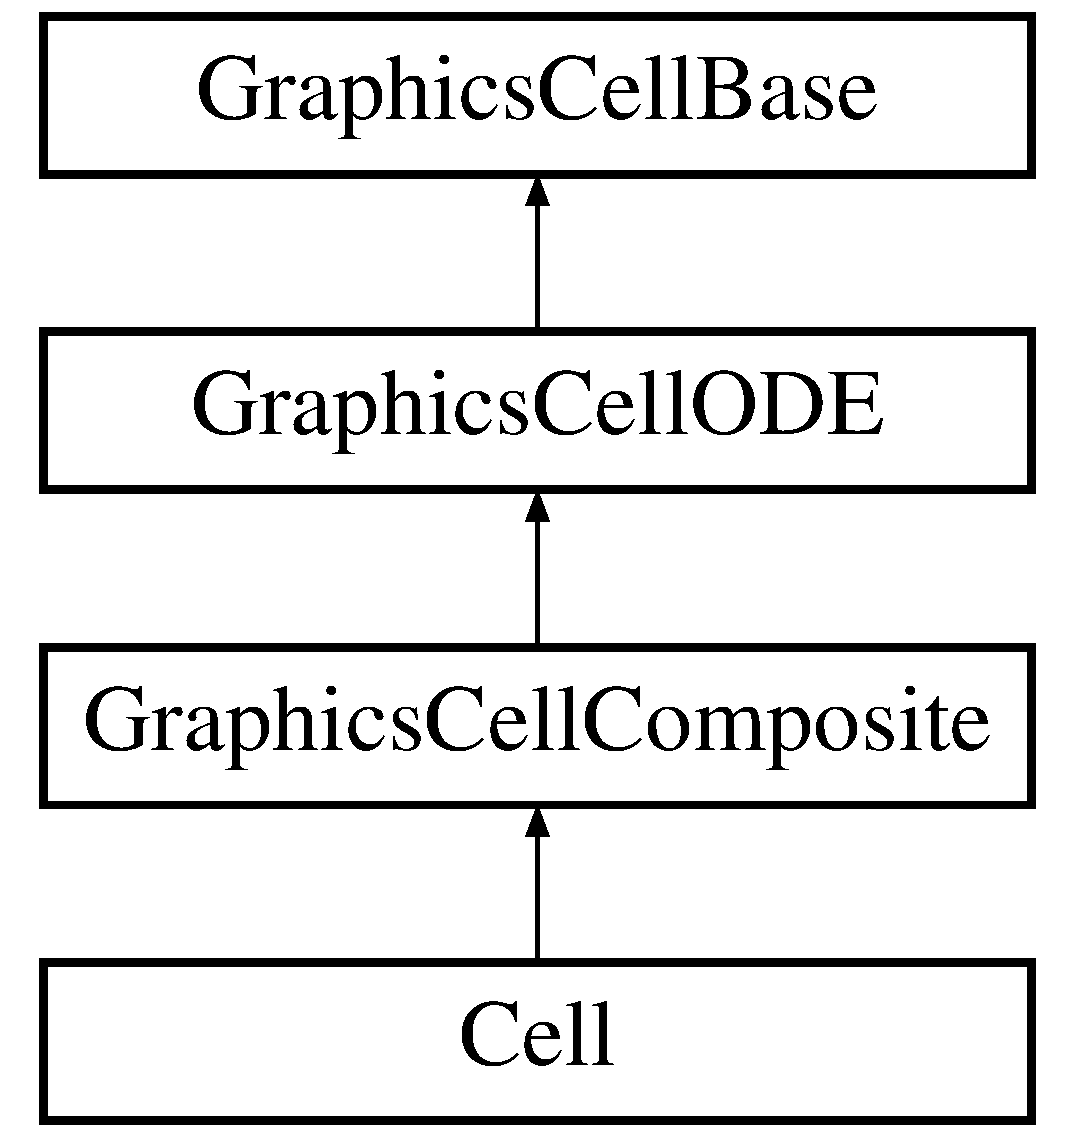
\includegraphics[height=4.000000cm]{class_graphics_cell_base}
\end{center}
\end{figure}
\subsection*{\-Public \-Member \-Functions}
\begin{DoxyCompactItemize}
\item 
int \hyperlink{class_graphics_cell_base_aaf51239fcc44325ad9cb828b96424033}{get\-Cell\-Index} () const 
\item 
float \hyperlink{class_graphics_cell_base_a0c638650a9cdbe65efdca7385d6f7454}{get\-Cell\-Length} () const 
\item 
float \hyperlink{class_graphics_cell_base_ab0a62023e5599c721fc4d6cad341785f}{get\-Cell\-Height} () const 
\item 
float \hyperlink{class_graphics_cell_base_ae9ce129f8462b6d05d9b52e504db27cf}{get\-Angle} () const 
\end{DoxyCompactItemize}
\subsection*{\-Protected \-Member \-Functions}
\begin{DoxyCompactItemize}
\item 
\hyperlink{class_graphics_cell_base_ab21c2ad274f163b192f0fc90317e71ce}{\-Graphics\-Cell\-Base} ()
\item 
\hyperlink{class_graphics_cell_base_a26ae84e6182edb34d86f82a31b01bf5c}{\-Graphics\-Cell\-Base} (const \hyperlink{class_graphics_cell_base}{\-Graphics\-Cell\-Base} \&cell)
\item 
\hyperlink{class_graphics_cell_base_a8ed7c2070beab9a56286df8dd8b36f12}{$\sim$\-Graphics\-Cell\-Base} ()
\item 
void \hyperlink{class_graphics_cell_base_a5f252a083de2b8d9a6ab3e38cd187c15}{copy} (const \hyperlink{class_graphics_cell_base}{\-Graphics\-Cell\-Base} \&c)
\item 
void \hyperlink{class_graphics_cell_base_a3a7ec63edecc54916e2770f233f97bc8}{set\-Cell\-Length} (float length)
\item 
void \hyperlink{class_graphics_cell_base_a78cfe59851d680ee459449dbd8befef7}{set\-Cell\-Height} (float height)
\item 
void \hyperlink{class_graphics_cell_base_a1bd5925a454cd3926652de53ce584f68}{set\-Cell\-Index} (int cell\-Index)
\item 
void \hyperlink{class_graphics_cell_base_a1b73509c13e0021bc01f28b481b3c649}{set\-Pos} (float x, float y, float z)
\item 
void \hyperlink{class_graphics_cell_base_aa23fb4905505dbd30f7f1a770a3a4e56}{set\-Angle} (float angle)
\end{DoxyCompactItemize}
\subsection*{\-Protected \-Attributes}
\begin{DoxyCompactItemize}
\item 
int \hyperlink{class_graphics_cell_base_abc8e8449329725e09994f29303133f1b}{cell\-Index\-\_\-}
\item 
float \hyperlink{class_graphics_cell_base_a4c4c5ffb768030b2cab10f28a1c62855}{angle\-\_\-}
\item 
float \hyperlink{class_graphics_cell_base_af802ab0cfb04f2ff82d1ae98e7c572ec}{cell\-Length\-\_\-}
\item 
float \hyperlink{class_graphics_cell_base_af4b0f90f9c14e984bf41f83e4733f214}{cell\-Height\-\_\-}
\item 
float \hyperlink{class_graphics_cell_base_a05f33e20efcbaf7be07c1267987c5dda}{cell\-Volume\-\_\-}
\item 
float \hyperlink{class_graphics_cell_base_a2159559ca4d11ec38456a52c8cb110ab}{pos\-X\-\_\-}
\item 
float \hyperlink{class_graphics_cell_base_a304771746db89eecb3f0c639cef8d412}{pos\-Y\-\_\-}
\item 
float \hyperlink{class_graphics_cell_base_af7b028e9b6a6950a95ab8b3355e05776}{pos\-Z\-\_\-}
\item 
bool \hyperlink{class_graphics_cell_base_ab8a1891eae9d2a1c0f24e1472f95b2c1}{has\-Focus\-\_\-}
\end{DoxyCompactItemize}


\subsection{\-Detailed \-Description}
\-Base class for the graphical representations of the cell. \-Define virtual functions as set position, update position, etc. 

\-Definition at line 35 of file \-Graphics\-Cell\-Base.\-h.



\subsection{\-Constructor \& \-Destructor \-Documentation}
\hypertarget{class_graphics_cell_base_ab21c2ad274f163b192f0fc90317e71ce}{\index{\-Graphics\-Cell\-Base@{\-Graphics\-Cell\-Base}!\-Graphics\-Cell\-Base@{\-Graphics\-Cell\-Base}}
\index{\-Graphics\-Cell\-Base@{\-Graphics\-Cell\-Base}!GraphicsCellBase@{\-Graphics\-Cell\-Base}}
\subsubsection[{\-Graphics\-Cell\-Base}]{\setlength{\rightskip}{0pt plus 5cm}{\bf \-Graphics\-Cell\-Base\-::\-Graphics\-Cell\-Base} (
\begin{DoxyParamCaption}
{}
\end{DoxyParamCaption}
)\hspace{0.3cm}{\ttfamily  \mbox{[}protected\mbox{]}}}}\label{class_graphics_cell_base_ab21c2ad274f163b192f0fc90317e71ce}


\-Definition at line 24 of file \-Graphics\-Cell\-Base.\-cpp.

\hypertarget{class_graphics_cell_base_a26ae84e6182edb34d86f82a31b01bf5c}{\index{\-Graphics\-Cell\-Base@{\-Graphics\-Cell\-Base}!\-Graphics\-Cell\-Base@{\-Graphics\-Cell\-Base}}
\index{\-Graphics\-Cell\-Base@{\-Graphics\-Cell\-Base}!GraphicsCellBase@{\-Graphics\-Cell\-Base}}
\subsubsection[{\-Graphics\-Cell\-Base}]{\setlength{\rightskip}{0pt plus 5cm}{\bf \-Graphics\-Cell\-Base\-::\-Graphics\-Cell\-Base} (
\begin{DoxyParamCaption}
\item[{const {\bf \-Graphics\-Cell\-Base} \&}]{cell}
\end{DoxyParamCaption}
)\hspace{0.3cm}{\ttfamily  \mbox{[}protected\mbox{]}}}}\label{class_graphics_cell_base_a26ae84e6182edb34d86f82a31b01bf5c}


\-Definition at line 37 of file \-Graphics\-Cell\-Base.\-cpp.

\hypertarget{class_graphics_cell_base_a8ed7c2070beab9a56286df8dd8b36f12}{\index{\-Graphics\-Cell\-Base@{\-Graphics\-Cell\-Base}!$\sim$\-Graphics\-Cell\-Base@{$\sim$\-Graphics\-Cell\-Base}}
\index{$\sim$\-Graphics\-Cell\-Base@{$\sim$\-Graphics\-Cell\-Base}!GraphicsCellBase@{\-Graphics\-Cell\-Base}}
\subsubsection[{$\sim$\-Graphics\-Cell\-Base}]{\setlength{\rightskip}{0pt plus 5cm}{\bf \-Graphics\-Cell\-Base\-::$\sim$\-Graphics\-Cell\-Base} (
\begin{DoxyParamCaption}
{}
\end{DoxyParamCaption}
)\hspace{0.3cm}{\ttfamily  \mbox{[}protected\mbox{]}}}}\label{class_graphics_cell_base_a8ed7c2070beab9a56286df8dd8b36f12}


\-Definition at line 20 of file \-Graphics\-Cell\-Base.\-cpp.



\subsection{\-Member \-Function \-Documentation}
\hypertarget{class_graphics_cell_base_a5f252a083de2b8d9a6ab3e38cd187c15}{\index{\-Graphics\-Cell\-Base@{\-Graphics\-Cell\-Base}!copy@{copy}}
\index{copy@{copy}!GraphicsCellBase@{\-Graphics\-Cell\-Base}}
\subsubsection[{copy}]{\setlength{\rightskip}{0pt plus 5cm}void {\bf \-Graphics\-Cell\-Base\-::copy} (
\begin{DoxyParamCaption}
\item[{const {\bf \-Graphics\-Cell\-Base} \&}]{c}
\end{DoxyParamCaption}
)\hspace{0.3cm}{\ttfamily  \mbox{[}protected\mbox{]}}}}\label{class_graphics_cell_base_a5f252a083de2b8d9a6ab3e38cd187c15}


\-Definition at line 44 of file \-Graphics\-Cell\-Base.\-cpp.

\hypertarget{class_graphics_cell_base_ae9ce129f8462b6d05d9b52e504db27cf}{\index{\-Graphics\-Cell\-Base@{\-Graphics\-Cell\-Base}!get\-Angle@{get\-Angle}}
\index{get\-Angle@{get\-Angle}!GraphicsCellBase@{\-Graphics\-Cell\-Base}}
\subsubsection[{get\-Angle}]{\setlength{\rightskip}{0pt plus 5cm}float {\bf \-Graphics\-Cell\-Base\-::get\-Angle} (
\begin{DoxyParamCaption}
{}
\end{DoxyParamCaption}
) const}}\label{class_graphics_cell_base_ae9ce129f8462b6d05d9b52e504db27cf}


\-Reimplemented in \hyperlink{class_cell_aaf492522ce24129fcac85bafb5dcc8f2}{\-Cell}, and \hyperlink{class_graphics_cell_o_d_e_a74aba3f28026f3ac58e19c92d26b170b}{\-Graphics\-Cell\-O\-D\-E}.



\-Definition at line 116 of file \-Graphics\-Cell\-Base.\-cpp.

\hypertarget{class_graphics_cell_base_ab0a62023e5599c721fc4d6cad341785f}{\index{\-Graphics\-Cell\-Base@{\-Graphics\-Cell\-Base}!get\-Cell\-Height@{get\-Cell\-Height}}
\index{get\-Cell\-Height@{get\-Cell\-Height}!GraphicsCellBase@{\-Graphics\-Cell\-Base}}
\subsubsection[{get\-Cell\-Height}]{\setlength{\rightskip}{0pt plus 5cm}float {\bf \-Graphics\-Cell\-Base\-::get\-Cell\-Height} (
\begin{DoxyParamCaption}
{}
\end{DoxyParamCaption}
) const}}\label{class_graphics_cell_base_ab0a62023e5599c721fc4d6cad341785f}


\-Definition at line 109 of file \-Graphics\-Cell\-Base.\-cpp.

\hypertarget{class_graphics_cell_base_aaf51239fcc44325ad9cb828b96424033}{\index{\-Graphics\-Cell\-Base@{\-Graphics\-Cell\-Base}!get\-Cell\-Index@{get\-Cell\-Index}}
\index{get\-Cell\-Index@{get\-Cell\-Index}!GraphicsCellBase@{\-Graphics\-Cell\-Base}}
\subsubsection[{get\-Cell\-Index}]{\setlength{\rightskip}{0pt plus 5cm}int {\bf \-Graphics\-Cell\-Base\-::get\-Cell\-Index} (
\begin{DoxyParamCaption}
{}
\end{DoxyParamCaption}
) const}}\label{class_graphics_cell_base_aaf51239fcc44325ad9cb828b96424033}


\-Definition at line 95 of file \-Graphics\-Cell\-Base.\-cpp.

\hypertarget{class_graphics_cell_base_a0c638650a9cdbe65efdca7385d6f7454}{\index{\-Graphics\-Cell\-Base@{\-Graphics\-Cell\-Base}!get\-Cell\-Length@{get\-Cell\-Length}}
\index{get\-Cell\-Length@{get\-Cell\-Length}!GraphicsCellBase@{\-Graphics\-Cell\-Base}}
\subsubsection[{get\-Cell\-Length}]{\setlength{\rightskip}{0pt plus 5cm}float {\bf \-Graphics\-Cell\-Base\-::get\-Cell\-Length} (
\begin{DoxyParamCaption}
{}
\end{DoxyParamCaption}
) const}}\label{class_graphics_cell_base_a0c638650a9cdbe65efdca7385d6f7454}


\-Definition at line 102 of file \-Graphics\-Cell\-Base.\-cpp.

\hypertarget{class_graphics_cell_base_aa23fb4905505dbd30f7f1a770a3a4e56}{\index{\-Graphics\-Cell\-Base@{\-Graphics\-Cell\-Base}!set\-Angle@{set\-Angle}}
\index{set\-Angle@{set\-Angle}!GraphicsCellBase@{\-Graphics\-Cell\-Base}}
\subsubsection[{set\-Angle}]{\setlength{\rightskip}{0pt plus 5cm}void {\bf \-Graphics\-Cell\-Base\-::set\-Angle} (
\begin{DoxyParamCaption}
\item[{float}]{angle}
\end{DoxyParamCaption}
)\hspace{0.3cm}{\ttfamily  \mbox{[}protected\mbox{]}}}}\label{class_graphics_cell_base_aa23fb4905505dbd30f7f1a770a3a4e56}


\-Reimplemented in \hyperlink{class_graphics_cell_o_d_e_aed881ba0ff5d4d14474e9dba8cde8045}{\-Graphics\-Cell\-O\-D\-E}, and \hyperlink{class_graphics_cell_composite_a28ceffaeac749a10742c70ce490b552c}{\-Graphics\-Cell\-Composite}.



\-Definition at line 88 of file \-Graphics\-Cell\-Base.\-cpp.

\hypertarget{class_graphics_cell_base_a78cfe59851d680ee459449dbd8befef7}{\index{\-Graphics\-Cell\-Base@{\-Graphics\-Cell\-Base}!set\-Cell\-Height@{set\-Cell\-Height}}
\index{set\-Cell\-Height@{set\-Cell\-Height}!GraphicsCellBase@{\-Graphics\-Cell\-Base}}
\subsubsection[{set\-Cell\-Height}]{\setlength{\rightskip}{0pt plus 5cm}void {\bf \-Graphics\-Cell\-Base\-::set\-Cell\-Height} (
\begin{DoxyParamCaption}
\item[{float}]{height}
\end{DoxyParamCaption}
)\hspace{0.3cm}{\ttfamily  \mbox{[}protected\mbox{]}}}}\label{class_graphics_cell_base_a78cfe59851d680ee459449dbd8befef7}


\-Reimplemented in \hyperlink{class_graphics_cell_o_d_e_af1a589ec827fcdbdb868a7abab7170d7}{\-Graphics\-Cell\-O\-D\-E}, and \hyperlink{class_graphics_cell_composite_a82373a1c4f0a6b53bd016da7d65313a3}{\-Graphics\-Cell\-Composite}.



\-Definition at line 65 of file \-Graphics\-Cell\-Base.\-cpp.

\hypertarget{class_graphics_cell_base_a1bd5925a454cd3926652de53ce584f68}{\index{\-Graphics\-Cell\-Base@{\-Graphics\-Cell\-Base}!set\-Cell\-Index@{set\-Cell\-Index}}
\index{set\-Cell\-Index@{set\-Cell\-Index}!GraphicsCellBase@{\-Graphics\-Cell\-Base}}
\subsubsection[{set\-Cell\-Index}]{\setlength{\rightskip}{0pt plus 5cm}void {\bf \-Graphics\-Cell\-Base\-::set\-Cell\-Index} (
\begin{DoxyParamCaption}
\item[{int}]{cell\-Index}
\end{DoxyParamCaption}
)\hspace{0.3cm}{\ttfamily  \mbox{[}protected\mbox{]}}}}\label{class_graphics_cell_base_a1bd5925a454cd3926652de53ce584f68}


\-Reimplemented in \hyperlink{class_cell_a8fa3d31ea4774884a1dd0ce488f14123}{\-Cell}.



\-Definition at line 72 of file \-Graphics\-Cell\-Base.\-cpp.

\hypertarget{class_graphics_cell_base_a3a7ec63edecc54916e2770f233f97bc8}{\index{\-Graphics\-Cell\-Base@{\-Graphics\-Cell\-Base}!set\-Cell\-Length@{set\-Cell\-Length}}
\index{set\-Cell\-Length@{set\-Cell\-Length}!GraphicsCellBase@{\-Graphics\-Cell\-Base}}
\subsubsection[{set\-Cell\-Length}]{\setlength{\rightskip}{0pt plus 5cm}void {\bf \-Graphics\-Cell\-Base\-::set\-Cell\-Length} (
\begin{DoxyParamCaption}
\item[{float}]{length}
\end{DoxyParamCaption}
)\hspace{0.3cm}{\ttfamily  \mbox{[}protected\mbox{]}}}}\label{class_graphics_cell_base_a3a7ec63edecc54916e2770f233f97bc8}


\-Reimplemented in \hyperlink{class_graphics_cell_o_d_e_a54402c3f0fd86ac188123913cc4cef37}{\-Graphics\-Cell\-O\-D\-E}, and \hyperlink{class_graphics_cell_composite_aafb153d72e30f23037c452547eb3c8fe}{\-Graphics\-Cell\-Composite}.



\-Definition at line 58 of file \-Graphics\-Cell\-Base.\-cpp.

\hypertarget{class_graphics_cell_base_a1b73509c13e0021bc01f28b481b3c649}{\index{\-Graphics\-Cell\-Base@{\-Graphics\-Cell\-Base}!set\-Pos@{set\-Pos}}
\index{set\-Pos@{set\-Pos}!GraphicsCellBase@{\-Graphics\-Cell\-Base}}
\subsubsection[{set\-Pos}]{\setlength{\rightskip}{0pt plus 5cm}void {\bf \-Graphics\-Cell\-Base\-::set\-Pos} (
\begin{DoxyParamCaption}
\item[{float}]{x, }
\item[{float}]{y, }
\item[{float}]{z}
\end{DoxyParamCaption}
)\hspace{0.3cm}{\ttfamily  \mbox{[}protected\mbox{]}}}}\label{class_graphics_cell_base_a1b73509c13e0021bc01f28b481b3c649}


\-Reimplemented in \hyperlink{class_graphics_cell_o_d_e_a952ed1d614c183406028a4eecd871135}{\-Graphics\-Cell\-O\-D\-E}.



\-Definition at line 79 of file \-Graphics\-Cell\-Base.\-cpp.



\subsection{\-Member \-Data \-Documentation}
\hypertarget{class_graphics_cell_base_a4c4c5ffb768030b2cab10f28a1c62855}{\index{\-Graphics\-Cell\-Base@{\-Graphics\-Cell\-Base}!angle\-\_\-@{angle\-\_\-}}
\index{angle\-\_\-@{angle\-\_\-}!GraphicsCellBase@{\-Graphics\-Cell\-Base}}
\subsubsection[{angle\-\_\-}]{\setlength{\rightskip}{0pt plus 5cm}float {\bf \-Graphics\-Cell\-Base\-::angle\-\_\-}\hspace{0.3cm}{\ttfamily  \mbox{[}protected\mbox{]}}}}\label{class_graphics_cell_base_a4c4c5ffb768030b2cab10f28a1c62855}


\-Definition at line 61 of file \-Graphics\-Cell\-Base.\-h.

\hypertarget{class_graphics_cell_base_af4b0f90f9c14e984bf41f83e4733f214}{\index{\-Graphics\-Cell\-Base@{\-Graphics\-Cell\-Base}!cell\-Height\-\_\-@{cell\-Height\-\_\-}}
\index{cell\-Height\-\_\-@{cell\-Height\-\_\-}!GraphicsCellBase@{\-Graphics\-Cell\-Base}}
\subsubsection[{cell\-Height\-\_\-}]{\setlength{\rightskip}{0pt plus 5cm}float {\bf \-Graphics\-Cell\-Base\-::cell\-Height\-\_\-}\hspace{0.3cm}{\ttfamily  \mbox{[}protected\mbox{]}}}}\label{class_graphics_cell_base_af4b0f90f9c14e984bf41f83e4733f214}
\hyperlink{class_cell}{\-Cell} height in microns. 

\-Definition at line 69 of file \-Graphics\-Cell\-Base.\-h.

\hypertarget{class_graphics_cell_base_abc8e8449329725e09994f29303133f1b}{\index{\-Graphics\-Cell\-Base@{\-Graphics\-Cell\-Base}!cell\-Index\-\_\-@{cell\-Index\-\_\-}}
\index{cell\-Index\-\_\-@{cell\-Index\-\_\-}!GraphicsCellBase@{\-Graphics\-Cell\-Base}}
\subsubsection[{cell\-Index\-\_\-}]{\setlength{\rightskip}{0pt plus 5cm}int {\bf \-Graphics\-Cell\-Base\-::cell\-Index\-\_\-}\hspace{0.3cm}{\ttfamily  \mbox{[}protected\mbox{]}}}}\label{class_graphics_cell_base_abc8e8449329725e09994f29303133f1b}


\-Definition at line 60 of file \-Graphics\-Cell\-Base.\-h.

\hypertarget{class_graphics_cell_base_af802ab0cfb04f2ff82d1ae98e7c572ec}{\index{\-Graphics\-Cell\-Base@{\-Graphics\-Cell\-Base}!cell\-Length\-\_\-@{cell\-Length\-\_\-}}
\index{cell\-Length\-\_\-@{cell\-Length\-\_\-}!GraphicsCellBase@{\-Graphics\-Cell\-Base}}
\subsubsection[{cell\-Length\-\_\-}]{\setlength{\rightskip}{0pt plus 5cm}float {\bf \-Graphics\-Cell\-Base\-::cell\-Length\-\_\-}\hspace{0.3cm}{\ttfamily  \mbox{[}protected\mbox{]}}}}\label{class_graphics_cell_base_af802ab0cfb04f2ff82d1ae98e7c572ec}
\hyperlink{class_cell}{\-Cell} length in microns. 

\-Definition at line 65 of file \-Graphics\-Cell\-Base.\-h.

\hypertarget{class_graphics_cell_base_a05f33e20efcbaf7be07c1267987c5dda}{\index{\-Graphics\-Cell\-Base@{\-Graphics\-Cell\-Base}!cell\-Volume\-\_\-@{cell\-Volume\-\_\-}}
\index{cell\-Volume\-\_\-@{cell\-Volume\-\_\-}!GraphicsCellBase@{\-Graphics\-Cell\-Base}}
\subsubsection[{cell\-Volume\-\_\-}]{\setlength{\rightskip}{0pt plus 5cm}float {\bf \-Graphics\-Cell\-Base\-::cell\-Volume\-\_\-}\hspace{0.3cm}{\ttfamily  \mbox{[}protected\mbox{]}}}}\label{class_graphics_cell_base_a05f33e20efcbaf7be07c1267987c5dda}


\-Definition at line 70 of file \-Graphics\-Cell\-Base.\-h.

\hypertarget{class_graphics_cell_base_ab8a1891eae9d2a1c0f24e1472f95b2c1}{\index{\-Graphics\-Cell\-Base@{\-Graphics\-Cell\-Base}!has\-Focus\-\_\-@{has\-Focus\-\_\-}}
\index{has\-Focus\-\_\-@{has\-Focus\-\_\-}!GraphicsCellBase@{\-Graphics\-Cell\-Base}}
\subsubsection[{has\-Focus\-\_\-}]{\setlength{\rightskip}{0pt plus 5cm}bool {\bf \-Graphics\-Cell\-Base\-::has\-Focus\-\_\-}\hspace{0.3cm}{\ttfamily  \mbox{[}protected\mbox{]}}}}\label{class_graphics_cell_base_ab8a1891eae9d2a1c0f24e1472f95b2c1}


\-Definition at line 74 of file \-Graphics\-Cell\-Base.\-h.

\hypertarget{class_graphics_cell_base_a2159559ca4d11ec38456a52c8cb110ab}{\index{\-Graphics\-Cell\-Base@{\-Graphics\-Cell\-Base}!pos\-X\-\_\-@{pos\-X\-\_\-}}
\index{pos\-X\-\_\-@{pos\-X\-\_\-}!GraphicsCellBase@{\-Graphics\-Cell\-Base}}
\subsubsection[{pos\-X\-\_\-}]{\setlength{\rightskip}{0pt plus 5cm}float {\bf \-Graphics\-Cell\-Base\-::pos\-X\-\_\-}\hspace{0.3cm}{\ttfamily  \mbox{[}protected\mbox{]}}}}\label{class_graphics_cell_base_a2159559ca4d11ec38456a52c8cb110ab}


\-Definition at line 71 of file \-Graphics\-Cell\-Base.\-h.

\hypertarget{class_graphics_cell_base_a304771746db89eecb3f0c639cef8d412}{\index{\-Graphics\-Cell\-Base@{\-Graphics\-Cell\-Base}!pos\-Y\-\_\-@{pos\-Y\-\_\-}}
\index{pos\-Y\-\_\-@{pos\-Y\-\_\-}!GraphicsCellBase@{\-Graphics\-Cell\-Base}}
\subsubsection[{pos\-Y\-\_\-}]{\setlength{\rightskip}{0pt plus 5cm}float {\bf \-Graphics\-Cell\-Base\-::pos\-Y\-\_\-}\hspace{0.3cm}{\ttfamily  \mbox{[}protected\mbox{]}}}}\label{class_graphics_cell_base_a304771746db89eecb3f0c639cef8d412}


\-Definition at line 72 of file \-Graphics\-Cell\-Base.\-h.

\hypertarget{class_graphics_cell_base_af7b028e9b6a6950a95ab8b3355e05776}{\index{\-Graphics\-Cell\-Base@{\-Graphics\-Cell\-Base}!pos\-Z\-\_\-@{pos\-Z\-\_\-}}
\index{pos\-Z\-\_\-@{pos\-Z\-\_\-}!GraphicsCellBase@{\-Graphics\-Cell\-Base}}
\subsubsection[{pos\-Z\-\_\-}]{\setlength{\rightskip}{0pt plus 5cm}float {\bf \-Graphics\-Cell\-Base\-::pos\-Z\-\_\-}\hspace{0.3cm}{\ttfamily  \mbox{[}protected\mbox{]}}}}\label{class_graphics_cell_base_af7b028e9b6a6950a95ab8b3355e05776}


\-Definition at line 73 of file \-Graphics\-Cell\-Base.\-h.



\-The documentation for this class was generated from the following files\-:\begin{DoxyCompactItemize}
\item 
/media/\-My\-Passport\-Blue/\-Data/\-Research/\-Simulations/\-Colony/\hyperlink{_graphics_cell_base_8h}{\-Graphics\-Cell\-Base.\-h}\item 
/media/\-My\-Passport\-Blue/\-Data/\-Research/\-Simulations/\-Colony/\hyperlink{_graphics_cell_base_8cpp}{\-Graphics\-Cell\-Base.\-cpp}\end{DoxyCompactItemize}

\hypertarget{class_graphics_cell_composite}{\section{\-Graphics\-Cell\-Composite \-Class \-Reference}
\label{class_graphics_cell_composite}\index{\-Graphics\-Cell\-Composite@{\-Graphics\-Cell\-Composite}}
}


{\ttfamily \#include $<$\-Graphics\-Cell\-Composite.\-h$>$}

\-Inheritance diagram for \-Graphics\-Cell\-Composite\-:\begin{figure}[H]
\begin{center}
\leavevmode
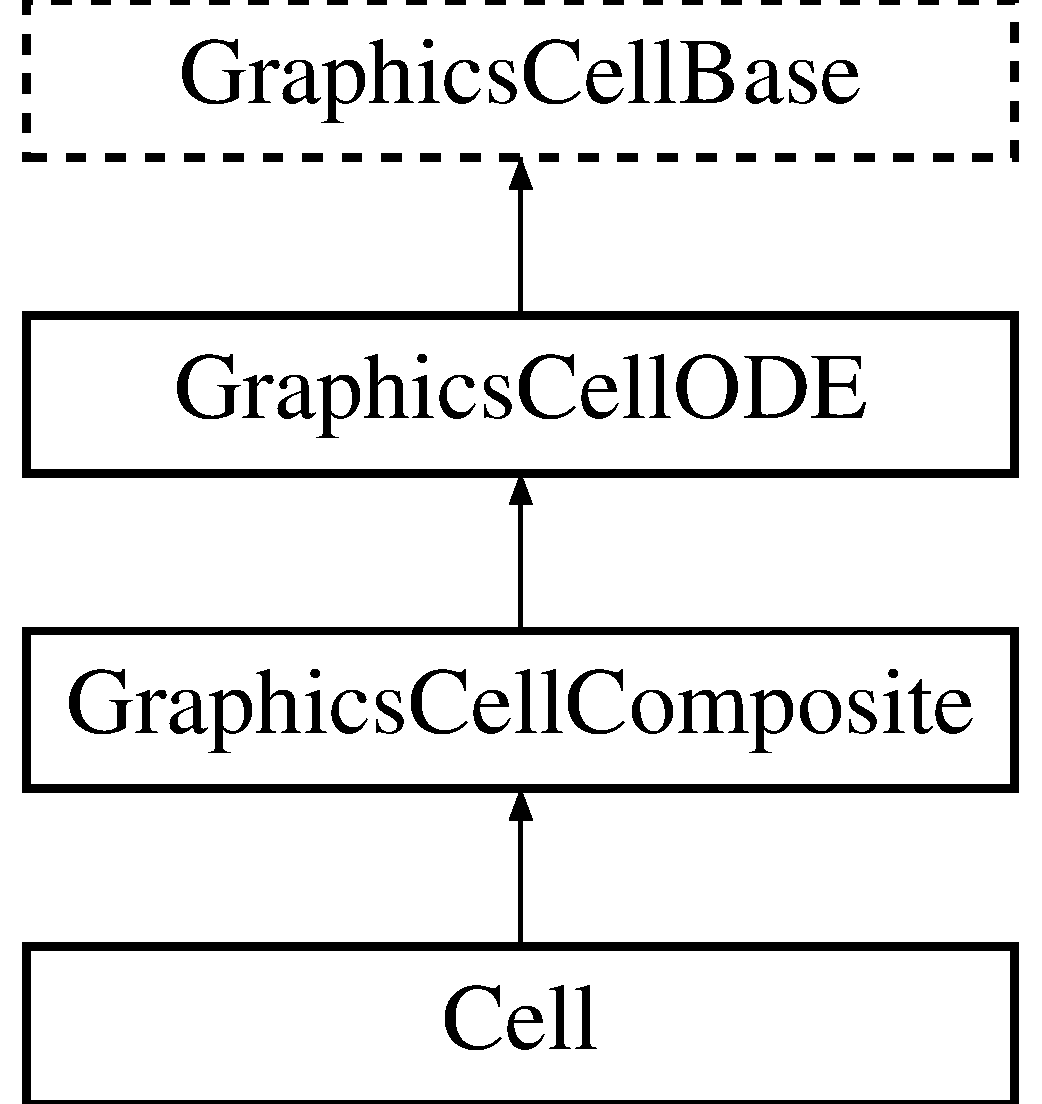
\includegraphics[height=4.000000cm]{class_graphics_cell_composite}
\end{center}
\end{figure}
\subsection*{\-Public \-Member \-Functions}
\begin{DoxyCompactItemize}
\item 
\hyperlink{class_graphics_cell_composite_a1c7ae93e329171a19a2a62b9220e1271}{\-Graphics\-Cell\-Composite} ()
\item 
\hyperlink{class_graphics_cell_composite_aabf09e89c4cc34389b15e70fd5d58db9}{\-Graphics\-Cell\-Composite} (const \hyperlink{class_graphics_cell_composite}{\-Graphics\-Cell\-Composite} \&cell)
\item 
\hyperlink{class_graphics_cell_composite_ae8f7c306f42815bba3e39b31c7fc8304}{$\sim$\-Graphics\-Cell\-Composite} ()
\item 
void \hyperlink{class_graphics_cell_composite_a062976e792a793aeb051d6fe0e951e06}{initialize} (\-Graphics\-Cell\-Composite\-Param \&p)
\item 
void \hyperlink{class_graphics_cell_composite_acc56ee3392352a6bd0d2ea943ceed031}{copy} (const \hyperlink{class_graphics_cell_composite}{\-Graphics\-Cell\-Composite} \&c)
\end{DoxyCompactItemize}
\subsection*{\-Protected \-Member \-Functions}
\begin{DoxyCompactItemize}
\item 
void \hyperlink{class_graphics_cell_composite_a26ea8e56ee5b43368423ac5b1097b4a8}{set\-Position} (float x, float y, float z)
\item 
void \hyperlink{class_graphics_cell_composite_a28ceffaeac749a10742c70ce490b552c}{set\-Angle} (float angle)
\item 
void \hyperlink{class_graphics_cell_composite_aafb153d72e30f23037c452547eb3c8fe}{set\-Cell\-Length} (float length)
\item 
void \hyperlink{class_graphics_cell_composite_a82373a1c4f0a6b53bd016da7d65313a3}{set\-Cell\-Height} (float height)
\end{DoxyCompactItemize}


\subsection{\-Detailed \-Description}


\-Definition at line 42 of file \-Graphics\-Cell\-Composite.\-h.



\subsection{\-Constructor \& \-Destructor \-Documentation}
\hypertarget{class_graphics_cell_composite_a1c7ae93e329171a19a2a62b9220e1271}{\index{\-Graphics\-Cell\-Composite@{\-Graphics\-Cell\-Composite}!\-Graphics\-Cell\-Composite@{\-Graphics\-Cell\-Composite}}
\index{\-Graphics\-Cell\-Composite@{\-Graphics\-Cell\-Composite}!GraphicsCellComposite@{\-Graphics\-Cell\-Composite}}
\subsubsection[{\-Graphics\-Cell\-Composite}]{\setlength{\rightskip}{0pt plus 5cm}{\bf \-Graphics\-Cell\-Composite\-::\-Graphics\-Cell\-Composite} (
\begin{DoxyParamCaption}
{}
\end{DoxyParamCaption}
)}}\label{class_graphics_cell_composite_a1c7ae93e329171a19a2a62b9220e1271}


\-Definition at line 24 of file \-Graphics\-Cell\-Composite.\-cpp.

\hypertarget{class_graphics_cell_composite_aabf09e89c4cc34389b15e70fd5d58db9}{\index{\-Graphics\-Cell\-Composite@{\-Graphics\-Cell\-Composite}!\-Graphics\-Cell\-Composite@{\-Graphics\-Cell\-Composite}}
\index{\-Graphics\-Cell\-Composite@{\-Graphics\-Cell\-Composite}!GraphicsCellComposite@{\-Graphics\-Cell\-Composite}}
\subsubsection[{\-Graphics\-Cell\-Composite}]{\setlength{\rightskip}{0pt plus 5cm}{\bf \-Graphics\-Cell\-Composite\-::\-Graphics\-Cell\-Composite} (
\begin{DoxyParamCaption}
\item[{const {\bf \-Graphics\-Cell\-Composite} \&}]{cell}
\end{DoxyParamCaption}
)}}\label{class_graphics_cell_composite_aabf09e89c4cc34389b15e70fd5d58db9}


\-Definition at line 37 of file \-Graphics\-Cell\-Composite.\-cpp.

\hypertarget{class_graphics_cell_composite_ae8f7c306f42815bba3e39b31c7fc8304}{\index{\-Graphics\-Cell\-Composite@{\-Graphics\-Cell\-Composite}!$\sim$\-Graphics\-Cell\-Composite@{$\sim$\-Graphics\-Cell\-Composite}}
\index{$\sim$\-Graphics\-Cell\-Composite@{$\sim$\-Graphics\-Cell\-Composite}!GraphicsCellComposite@{\-Graphics\-Cell\-Composite}}
\subsubsection[{$\sim$\-Graphics\-Cell\-Composite}]{\setlength{\rightskip}{0pt plus 5cm}{\bf \-Graphics\-Cell\-Composite\-::$\sim$\-Graphics\-Cell\-Composite} (
\begin{DoxyParamCaption}
{}
\end{DoxyParamCaption}
)}}\label{class_graphics_cell_composite_ae8f7c306f42815bba3e39b31c7fc8304}


\-Definition at line 20 of file \-Graphics\-Cell\-Composite.\-cpp.



\subsection{\-Member \-Function \-Documentation}
\hypertarget{class_graphics_cell_composite_acc56ee3392352a6bd0d2ea943ceed031}{\index{\-Graphics\-Cell\-Composite@{\-Graphics\-Cell\-Composite}!copy@{copy}}
\index{copy@{copy}!GraphicsCellComposite@{\-Graphics\-Cell\-Composite}}
\subsubsection[{copy}]{\setlength{\rightskip}{0pt plus 5cm}void {\bf \-Graphics\-Cell\-Composite\-::copy} (
\begin{DoxyParamCaption}
\item[{const {\bf \-Graphics\-Cell\-Composite} \&}]{c}
\end{DoxyParamCaption}
)}}\label{class_graphics_cell_composite_acc56ee3392352a6bd0d2ea943ceed031}


\-Definition at line 54 of file \-Graphics\-Cell\-Composite.\-cpp.

\hypertarget{class_graphics_cell_composite_a062976e792a793aeb051d6fe0e951e06}{\index{\-Graphics\-Cell\-Composite@{\-Graphics\-Cell\-Composite}!initialize@{initialize}}
\index{initialize@{initialize}!GraphicsCellComposite@{\-Graphics\-Cell\-Composite}}
\subsubsection[{initialize}]{\setlength{\rightskip}{0pt plus 5cm}void {\bf \-Graphics\-Cell\-Composite\-::initialize} (
\begin{DoxyParamCaption}
\item[{\-Graphics\-Cell\-Composite\-Param \&}]{p}
\end{DoxyParamCaption}
)}}\label{class_graphics_cell_composite_a062976e792a793aeb051d6fe0e951e06}


\-Definition at line 71 of file \-Graphics\-Cell\-Composite.\-cpp.

\hypertarget{class_graphics_cell_composite_a28ceffaeac749a10742c70ce490b552c}{\index{\-Graphics\-Cell\-Composite@{\-Graphics\-Cell\-Composite}!set\-Angle@{set\-Angle}}
\index{set\-Angle@{set\-Angle}!GraphicsCellComposite@{\-Graphics\-Cell\-Composite}}
\subsubsection[{set\-Angle}]{\setlength{\rightskip}{0pt plus 5cm}void {\bf \-Graphics\-Cell\-Composite\-::set\-Angle} (
\begin{DoxyParamCaption}
\item[{float}]{angle}
\end{DoxyParamCaption}
)\hspace{0.3cm}{\ttfamily  \mbox{[}protected\mbox{]}}}}\label{class_graphics_cell_composite_a28ceffaeac749a10742c70ce490b552c}


\-Reimplemented from \hyperlink{class_graphics_cell_o_d_e_aed881ba0ff5d4d14474e9dba8cde8045}{\-Graphics\-Cell\-O\-D\-E}.



\-Definition at line 116 of file \-Graphics\-Cell\-Composite.\-cpp.

\hypertarget{class_graphics_cell_composite_a82373a1c4f0a6b53bd016da7d65313a3}{\index{\-Graphics\-Cell\-Composite@{\-Graphics\-Cell\-Composite}!set\-Cell\-Height@{set\-Cell\-Height}}
\index{set\-Cell\-Height@{set\-Cell\-Height}!GraphicsCellComposite@{\-Graphics\-Cell\-Composite}}
\subsubsection[{set\-Cell\-Height}]{\setlength{\rightskip}{0pt plus 5cm}void {\bf \-Graphics\-Cell\-Composite\-::set\-Cell\-Height} (
\begin{DoxyParamCaption}
\item[{float}]{height}
\end{DoxyParamCaption}
)\hspace{0.3cm}{\ttfamily  \mbox{[}protected\mbox{]}}}}\label{class_graphics_cell_composite_a82373a1c4f0a6b53bd016da7d65313a3}


\-Reimplemented from \hyperlink{class_graphics_cell_o_d_e_af1a589ec827fcdbdb868a7abab7170d7}{\-Graphics\-Cell\-O\-D\-E}.



\-Definition at line 163 of file \-Graphics\-Cell\-Composite.\-cpp.

\hypertarget{class_graphics_cell_composite_aafb153d72e30f23037c452547eb3c8fe}{\index{\-Graphics\-Cell\-Composite@{\-Graphics\-Cell\-Composite}!set\-Cell\-Length@{set\-Cell\-Length}}
\index{set\-Cell\-Length@{set\-Cell\-Length}!GraphicsCellComposite@{\-Graphics\-Cell\-Composite}}
\subsubsection[{set\-Cell\-Length}]{\setlength{\rightskip}{0pt plus 5cm}void {\bf \-Graphics\-Cell\-Composite\-::set\-Cell\-Length} (
\begin{DoxyParamCaption}
\item[{float}]{length}
\end{DoxyParamCaption}
)\hspace{0.3cm}{\ttfamily  \mbox{[}protected\mbox{]}}}}\label{class_graphics_cell_composite_aafb153d72e30f23037c452547eb3c8fe}


\-Reimplemented from \hyperlink{class_graphics_cell_o_d_e_a54402c3f0fd86ac188123913cc4cef37}{\-Graphics\-Cell\-O\-D\-E}.



\-Definition at line 145 of file \-Graphics\-Cell\-Composite.\-cpp.

\hypertarget{class_graphics_cell_composite_a26ea8e56ee5b43368423ac5b1097b4a8}{\index{\-Graphics\-Cell\-Composite@{\-Graphics\-Cell\-Composite}!set\-Position@{set\-Position}}
\index{set\-Position@{set\-Position}!GraphicsCellComposite@{\-Graphics\-Cell\-Composite}}
\subsubsection[{set\-Position}]{\setlength{\rightskip}{0pt plus 5cm}void {\bf \-Graphics\-Cell\-Composite\-::set\-Position} (
\begin{DoxyParamCaption}
\item[{float}]{x, }
\item[{float}]{y, }
\item[{float}]{z}
\end{DoxyParamCaption}
)\hspace{0.3cm}{\ttfamily  \mbox{[}protected\mbox{]}}}}\label{class_graphics_cell_composite_a26ea8e56ee5b43368423ac5b1097b4a8}


\-Definition at line 88 of file \-Graphics\-Cell\-Composite.\-cpp.



\-The documentation for this class was generated from the following files\-:\begin{DoxyCompactItemize}
\item 
/media/\-My\-Passport\-Blue/\-Data/\-Research/\-Simulations/\-Colony/\hyperlink{_graphics_cell_composite_8h}{\-Graphics\-Cell\-Composite.\-h}\item 
/media/\-My\-Passport\-Blue/\-Data/\-Research/\-Simulations/\-Colony/\hyperlink{_graphics_cell_composite_8cpp}{\-Graphics\-Cell\-Composite.\-cpp}\end{DoxyCompactItemize}

\hypertarget{class_graphics_cell_o_d_e}{\section{\-Graphics\-Cell\-O\-D\-E \-Class \-Reference}
\label{class_graphics_cell_o_d_e}\index{\-Graphics\-Cell\-O\-D\-E@{\-Graphics\-Cell\-O\-D\-E}}
}


{\ttfamily \#include $<$\-Graphics\-Cell\-O\-D\-E.\-h$>$}

\-Inheritance diagram for \-Graphics\-Cell\-O\-D\-E\-:\begin{figure}[H]
\begin{center}
\leavevmode
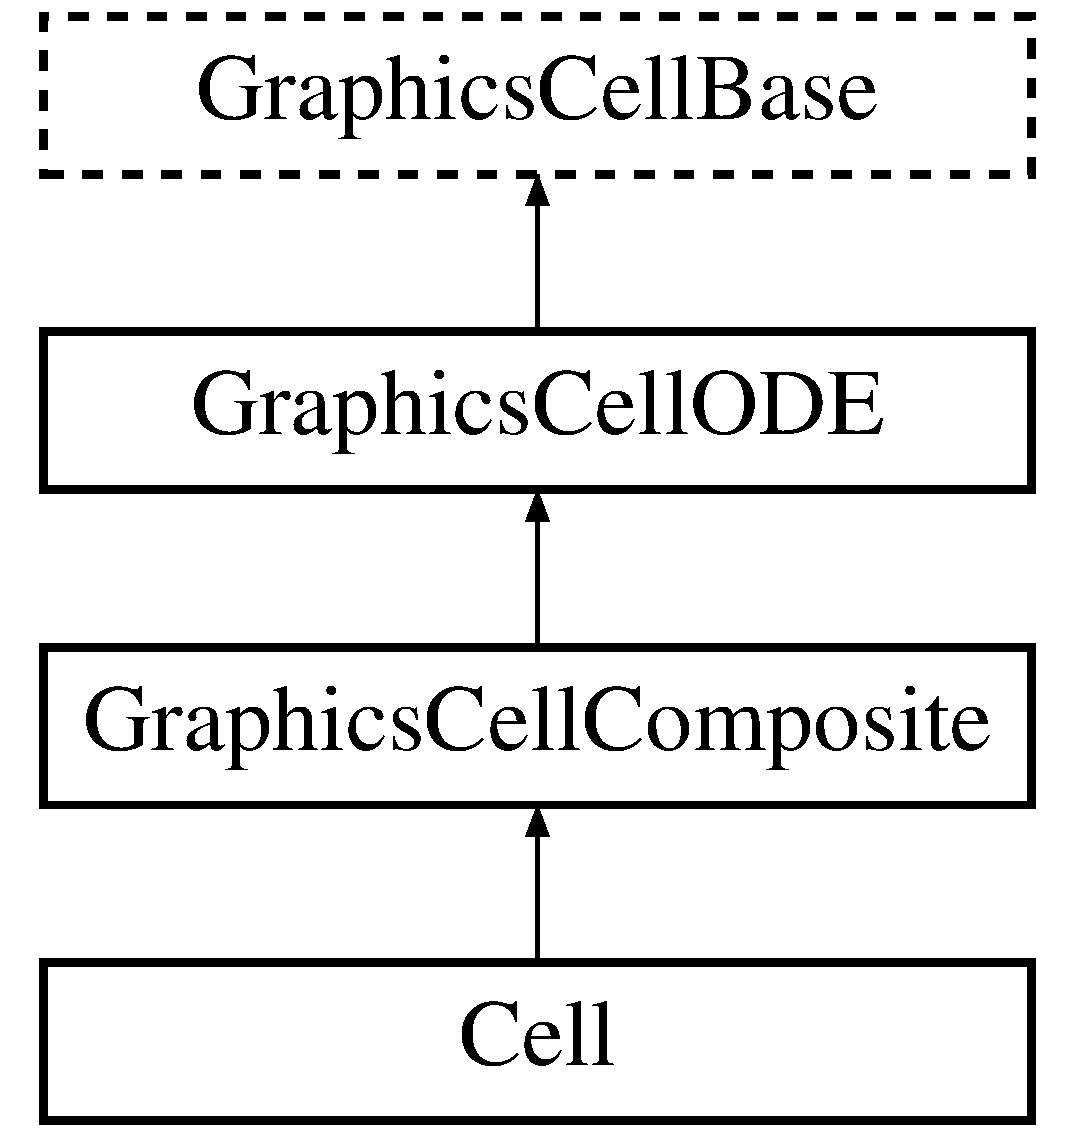
\includegraphics[height=4.000000cm]{class_graphics_cell_o_d_e}
\end{center}
\end{figure}
\subsection*{\-Public \-Member \-Functions}
\begin{DoxyCompactItemize}
\item 
\hyperlink{class_graphics_cell_o_d_e_a62316d8bfd6011407f62c78f4530e415}{\-Graphics\-Cell\-O\-D\-E} ()
\item 
\hyperlink{class_graphics_cell_o_d_e_aa11de20bcd4975c8066adb71afa02d74}{\-Graphics\-Cell\-O\-D\-E} (const \hyperlink{class_graphics_cell_o_d_e}{\-Graphics\-Cell\-O\-D\-E} \&cell)
\item 
\hyperlink{class_graphics_cell_o_d_e_a77528d47f270929cc50f75226e36df5d}{$\sim$\-Graphics\-Cell\-O\-D\-E} ()
\item 
void \hyperlink{class_graphics_cell_o_d_e_a5ed31da765f83ab4d0803d3181564867}{initialize} (d\-World\-I\-D world, d\-Space\-I\-D space, \hyperlink{class_spatial_integrator_o_d_e}{\-Spatial\-Integrator\-O\-D\-E} $\ast$spatial\-Integrator\-O\-D\-E)
\item 
void \hyperlink{class_graphics_cell_o_d_e_acbba71e955bd7b7f1c23776073285121}{copy} (const \hyperlink{class_graphics_cell_o_d_e}{\-Graphics\-Cell\-O\-D\-E} \&cell)
\item 
d\-World\-I\-D \hyperlink{class_graphics_cell_o_d_e_a56cb145cb7f9835601de35fbe90c5719}{get\-World} () const 
\item 
d\-Space\-I\-D \hyperlink{class_graphics_cell_o_d_e_aff5270931c0b33a6be68171c9e565f6d}{get\-Space} () const 
\item 
d\-Body\-I\-D \hyperlink{class_graphics_cell_o_d_e_a30c7bb1b68d60a97b910186785510751}{get\-Body} ()
\item 
double \hyperlink{class_graphics_cell_o_d_e_a74aba3f28026f3ac58e19c92d26b170b}{get\-Angle} () const 
\item 
\-Tiny\-Vector$<$ double, 3 $>$ \hyperlink{class_graphics_cell_o_d_e_a1c3da62e9a9c096155a4dcc23e4686fa}{get\-Position\-O\-D\-E} () const 
\item 
void \hyperlink{class_graphics_cell_o_d_e_a799fbb19bd9fd536df75a9783539afc0}{align\-To\-Z\-Axis} ()
\item 
void \hyperlink{class_graphics_cell_o_d_e_aa895e22390a23f83ad33579a8440661e}{limit\-Velocity} (float max\-Velocity\-Squared, float max\-Rot\-Velocity\-Squared)
\end{DoxyCompactItemize}
\subsection*{\-Protected \-Member \-Functions}
\begin{DoxyCompactItemize}
\item 
void \hyperlink{class_graphics_cell_o_d_e_a952ed1d614c183406028a4eecd871135}{set\-Pos} (float x, float y, float z)
\item 
void \hyperlink{class_graphics_cell_o_d_e_aed881ba0ff5d4d14474e9dba8cde8045}{set\-Angle} (float angle)
\item 
void \hyperlink{class_graphics_cell_o_d_e_a54402c3f0fd86ac188123913cc4cef37}{set\-Cell\-Length} (float length)
\item 
void \hyperlink{class_graphics_cell_o_d_e_af1a589ec827fcdbdb868a7abab7170d7}{set\-Cell\-Height} (float height)
\item 
void \hyperlink{class_graphics_cell_o_d_e_a6f157aeac8e7e6260d7e77c72b3936c9}{update\-Geometry} ()
\end{DoxyCompactItemize}


\subsection{\-Detailed \-Description}
\-Cell as \-O\-D\-E object definition. 

\-Definition at line 39 of file \-Graphics\-Cell\-O\-D\-E.\-h.



\subsection{\-Constructor \& \-Destructor \-Documentation}
\hypertarget{class_graphics_cell_o_d_e_a62316d8bfd6011407f62c78f4530e415}{\index{\-Graphics\-Cell\-O\-D\-E@{\-Graphics\-Cell\-O\-D\-E}!\-Graphics\-Cell\-O\-D\-E@{\-Graphics\-Cell\-O\-D\-E}}
\index{\-Graphics\-Cell\-O\-D\-E@{\-Graphics\-Cell\-O\-D\-E}!GraphicsCellODE@{\-Graphics\-Cell\-O\-D\-E}}
\subsubsection[{\-Graphics\-Cell\-O\-D\-E}]{\setlength{\rightskip}{0pt plus 5cm}{\bf \-Graphics\-Cell\-O\-D\-E\-::\-Graphics\-Cell\-O\-D\-E} (
\begin{DoxyParamCaption}
{}
\end{DoxyParamCaption}
)}}\label{class_graphics_cell_o_d_e_a62316d8bfd6011407f62c78f4530e415}


\-Definition at line 21 of file \-Graphics\-Cell\-O\-D\-E.\-cpp.

\hypertarget{class_graphics_cell_o_d_e_aa11de20bcd4975c8066adb71afa02d74}{\index{\-Graphics\-Cell\-O\-D\-E@{\-Graphics\-Cell\-O\-D\-E}!\-Graphics\-Cell\-O\-D\-E@{\-Graphics\-Cell\-O\-D\-E}}
\index{\-Graphics\-Cell\-O\-D\-E@{\-Graphics\-Cell\-O\-D\-E}!GraphicsCellODE@{\-Graphics\-Cell\-O\-D\-E}}
\subsubsection[{\-Graphics\-Cell\-O\-D\-E}]{\setlength{\rightskip}{0pt plus 5cm}{\bf \-Graphics\-Cell\-O\-D\-E\-::\-Graphics\-Cell\-O\-D\-E} (
\begin{DoxyParamCaption}
\item[{const {\bf \-Graphics\-Cell\-O\-D\-E} \&}]{cell}
\end{DoxyParamCaption}
)}}\label{class_graphics_cell_o_d_e_aa11de20bcd4975c8066adb71afa02d74}


\-Definition at line 85 of file \-Graphics\-Cell\-O\-D\-E.\-cpp.

\hypertarget{class_graphics_cell_o_d_e_a77528d47f270929cc50f75226e36df5d}{\index{\-Graphics\-Cell\-O\-D\-E@{\-Graphics\-Cell\-O\-D\-E}!$\sim$\-Graphics\-Cell\-O\-D\-E@{$\sim$\-Graphics\-Cell\-O\-D\-E}}
\index{$\sim$\-Graphics\-Cell\-O\-D\-E@{$\sim$\-Graphics\-Cell\-O\-D\-E}!GraphicsCellODE@{\-Graphics\-Cell\-O\-D\-E}}
\subsubsection[{$\sim$\-Graphics\-Cell\-O\-D\-E}]{\setlength{\rightskip}{0pt plus 5cm}{\bf \-Graphics\-Cell\-O\-D\-E\-::$\sim$\-Graphics\-Cell\-O\-D\-E} (
\begin{DoxyParamCaption}
{}
\end{DoxyParamCaption}
)}}\label{class_graphics_cell_o_d_e_a77528d47f270929cc50f75226e36df5d}
\-Delete reference in the list of cell in \hyperlink{class_spatial_integrator_o_d_e}{\-Spatial\-Integrator\-O\-D\-E} class. 

\-Definition at line 27 of file \-Graphics\-Cell\-O\-D\-E.\-cpp.



\subsection{\-Member \-Function \-Documentation}
\hypertarget{class_graphics_cell_o_d_e_a799fbb19bd9fd536df75a9783539afc0}{\index{\-Graphics\-Cell\-O\-D\-E@{\-Graphics\-Cell\-O\-D\-E}!align\-To\-Z\-Axis@{align\-To\-Z\-Axis}}
\index{align\-To\-Z\-Axis@{align\-To\-Z\-Axis}!GraphicsCellODE@{\-Graphics\-Cell\-O\-D\-E}}
\subsubsection[{align\-To\-Z\-Axis}]{\setlength{\rightskip}{0pt plus 5cm}void {\bf \-Graphics\-Cell\-O\-D\-E\-::align\-To\-Z\-Axis} (
\begin{DoxyParamCaption}
{}
\end{DoxyParamCaption}
)}}\label{class_graphics_cell_o_d_e_a799fbb19bd9fd536df75a9783539afc0}
\-Correct the angular velocity and rotation matrix to verify the xy plane constrain. 

\-Definition at line 298 of file \-Graphics\-Cell\-O\-D\-E.\-cpp.

\hypertarget{class_graphics_cell_o_d_e_acbba71e955bd7b7f1c23776073285121}{\index{\-Graphics\-Cell\-O\-D\-E@{\-Graphics\-Cell\-O\-D\-E}!copy@{copy}}
\index{copy@{copy}!GraphicsCellODE@{\-Graphics\-Cell\-O\-D\-E}}
\subsubsection[{copy}]{\setlength{\rightskip}{0pt plus 5cm}void {\bf \-Graphics\-Cell\-O\-D\-E\-::copy} (
\begin{DoxyParamCaption}
\item[{const {\bf \-Graphics\-Cell\-O\-D\-E} \&}]{cell}
\end{DoxyParamCaption}
)}}\label{class_graphics_cell_o_d_e_acbba71e955bd7b7f1c23776073285121}

\begin{DoxyItemize}
\item \-Set the \-O\-D\-E world and space.
\end{DoxyItemize}


\begin{DoxyItemize}
\item \-Get body position and orientation.
\end{DoxyItemize}


\begin{DoxyItemize}
\item \-Get the body linear velocity and angular velocity.
\end{DoxyItemize}


\begin{DoxyItemize}
\item \-Get the cell height from the \-Graphics\-Cell object.
\end{DoxyItemize}


\begin{DoxyItemize}
\item \-Initiate geometry (object shape).
\end{DoxyItemize}


\begin{DoxyItemize}
\item \-Initiate body (mass, inertia).
\end{DoxyItemize}


\begin{DoxyItemize}
\item \-Associate body and geometry.
\end{DoxyItemize}


\begin{DoxyItemize}
\item \-Set geometry and body position to the same as before.
\end{DoxyItemize}


\begin{DoxyItemize}
\item \-Set geometry and body rotation to the same as before.
\end{DoxyItemize}


\begin{DoxyItemize}
\item \-Set geometry and body linear velocity to the same as before.
\end{DoxyItemize}


\begin{DoxyItemize}
\item \-Set geometry and body angular velocity to the same as before.
\end{DoxyItemize}


\begin{DoxyItemize}
\item \-Restrict movement to the plane.
\end{DoxyItemize}


\begin{DoxyItemize}
\item \-Add the cell to the list in the spatial\-Integrator\-O\-D\-E 
\end{DoxyItemize}

\-Definition at line 92 of file \-Graphics\-Cell\-O\-D\-E.\-cpp.

\hypertarget{class_graphics_cell_o_d_e_a74aba3f28026f3ac58e19c92d26b170b}{\index{\-Graphics\-Cell\-O\-D\-E@{\-Graphics\-Cell\-O\-D\-E}!get\-Angle@{get\-Angle}}
\index{get\-Angle@{get\-Angle}!GraphicsCellODE@{\-Graphics\-Cell\-O\-D\-E}}
\subsubsection[{get\-Angle}]{\setlength{\rightskip}{0pt plus 5cm}double {\bf \-Graphics\-Cell\-O\-D\-E\-::get\-Angle} (
\begin{DoxyParamCaption}
{}
\end{DoxyParamCaption}
) const}}\label{class_graphics_cell_o_d_e_a74aba3f28026f3ac58e19c92d26b170b}

\begin{DoxyItemize}
\item \-Get the quaternion matrix of the \-O\-D\-E geometry.
\end{DoxyItemize}


\begin{DoxyItemize}
\item \-Remark\-: a quaternion is equal to (cos(alpha/2),sin(alpha/2)$\ast$u), where u is a unit vector of the rotation axis.
\begin{DoxyItemize}
\item \-Remark\-: the rotation axis should already be in the xy plane and the rotation angle should be 90 degrees.
\end{DoxyItemize}
\end{DoxyItemize}


\begin{DoxyItemize}
\item \-Calculate the orientation of the rotation axis in the xy plane, \-Euler psi angle.
\end{DoxyItemize}


\begin{DoxyItemize}
\item \-The orientation of the cell is perpendicular to the rotation axis.
\end{DoxyItemize}


\begin{DoxyItemize}
\item \-Transform from radians to degrees. 
\end{DoxyItemize}

\-Reimplemented from \hyperlink{class_graphics_cell_base_ae9ce129f8462b6d05d9b52e504db27cf}{\-Graphics\-Cell\-Base}.



\-Reimplemented in \hyperlink{class_cell_aaf492522ce24129fcac85bafb5dcc8f2}{\-Cell}.



\-Definition at line 275 of file \-Graphics\-Cell\-O\-D\-E.\-cpp.

\hypertarget{class_graphics_cell_o_d_e_a30c7bb1b68d60a97b910186785510751}{\index{\-Graphics\-Cell\-O\-D\-E@{\-Graphics\-Cell\-O\-D\-E}!get\-Body@{get\-Body}}
\index{get\-Body@{get\-Body}!GraphicsCellODE@{\-Graphics\-Cell\-O\-D\-E}}
\subsubsection[{get\-Body}]{\setlength{\rightskip}{0pt plus 5cm}d\-Body\-I\-D {\bf \-Graphics\-Cell\-O\-D\-E\-::get\-Body} (
\begin{DoxyParamCaption}
{}
\end{DoxyParamCaption}
)}}\label{class_graphics_cell_o_d_e_a30c7bb1b68d60a97b910186785510751}


\-Definition at line 256 of file \-Graphics\-Cell\-O\-D\-E.\-cpp.

\hypertarget{class_graphics_cell_o_d_e_a1c3da62e9a9c096155a4dcc23e4686fa}{\index{\-Graphics\-Cell\-O\-D\-E@{\-Graphics\-Cell\-O\-D\-E}!get\-Position\-O\-D\-E@{get\-Position\-O\-D\-E}}
\index{get\-Position\-O\-D\-E@{get\-Position\-O\-D\-E}!GraphicsCellODE@{\-Graphics\-Cell\-O\-D\-E}}
\subsubsection[{get\-Position\-O\-D\-E}]{\setlength{\rightskip}{0pt plus 5cm}\-Tiny\-Vector$<$ double, 3 $>$ {\bf \-Graphics\-Cell\-O\-D\-E\-::get\-Position\-O\-D\-E} (
\begin{DoxyParamCaption}
{}
\end{DoxyParamCaption}
) const}}\label{class_graphics_cell_o_d_e_a1c3da62e9a9c096155a4dcc23e4686fa}


\-Definition at line 263 of file \-Graphics\-Cell\-O\-D\-E.\-cpp.

\hypertarget{class_graphics_cell_o_d_e_aff5270931c0b33a6be68171c9e565f6d}{\index{\-Graphics\-Cell\-O\-D\-E@{\-Graphics\-Cell\-O\-D\-E}!get\-Space@{get\-Space}}
\index{get\-Space@{get\-Space}!GraphicsCellODE@{\-Graphics\-Cell\-O\-D\-E}}
\subsubsection[{get\-Space}]{\setlength{\rightskip}{0pt plus 5cm}d\-Space\-I\-D {\bf \-Graphics\-Cell\-O\-D\-E\-::get\-Space} (
\begin{DoxyParamCaption}
{}
\end{DoxyParamCaption}
) const}}\label{class_graphics_cell_o_d_e_aff5270931c0b33a6be68171c9e565f6d}


\-Definition at line 249 of file \-Graphics\-Cell\-O\-D\-E.\-cpp.

\hypertarget{class_graphics_cell_o_d_e_a56cb145cb7f9835601de35fbe90c5719}{\index{\-Graphics\-Cell\-O\-D\-E@{\-Graphics\-Cell\-O\-D\-E}!get\-World@{get\-World}}
\index{get\-World@{get\-World}!GraphicsCellODE@{\-Graphics\-Cell\-O\-D\-E}}
\subsubsection[{get\-World}]{\setlength{\rightskip}{0pt plus 5cm}d\-World\-I\-D {\bf \-Graphics\-Cell\-O\-D\-E\-::get\-World} (
\begin{DoxyParamCaption}
{}
\end{DoxyParamCaption}
) const}}\label{class_graphics_cell_o_d_e_a56cb145cb7f9835601de35fbe90c5719}


\-Definition at line 242 of file \-Graphics\-Cell\-O\-D\-E.\-cpp.

\hypertarget{class_graphics_cell_o_d_e_a5ed31da765f83ab4d0803d3181564867}{\index{\-Graphics\-Cell\-O\-D\-E@{\-Graphics\-Cell\-O\-D\-E}!initialize@{initialize}}
\index{initialize@{initialize}!GraphicsCellODE@{\-Graphics\-Cell\-O\-D\-E}}
\subsubsection[{initialize}]{\setlength{\rightskip}{0pt plus 5cm}void {\bf \-Graphics\-Cell\-O\-D\-E\-::initialize} (
\begin{DoxyParamCaption}
\item[{d\-World\-I\-D}]{world, }
\item[{d\-Space\-I\-D}]{space, }
\item[{{\bf \-Spatial\-Integrator\-O\-D\-E} $\ast$}]{spatial\-Integrator\-O\-D\-E}
\end{DoxyParamCaption}
)}}\label{class_graphics_cell_o_d_e_a5ed31da765f83ab4d0803d3181564867}

\begin{DoxyItemize}
\item \-Set the \-O\-D\-E world and space.
\end{DoxyItemize}


\begin{DoxyItemize}
\item \-Get the cell height from the \-Graphics\-Cell object.
\end{DoxyItemize}


\begin{DoxyItemize}
\item \-Initiate body (mass, inertia).
\end{DoxyItemize}


\begin{DoxyItemize}
\item \-Associate body and geometry.
\end{DoxyItemize}


\begin{DoxyItemize}
\item \-Restrict movement to the plane.
\end{DoxyItemize}


\begin{DoxyItemize}
\item \-Add the cell to the list in the spatial\-Integrator\-O\-D\-E 
\end{DoxyItemize}

\-Definition at line 43 of file \-Graphics\-Cell\-O\-D\-E.\-cpp.

\hypertarget{class_graphics_cell_o_d_e_aa895e22390a23f83ad33579a8440661e}{\index{\-Graphics\-Cell\-O\-D\-E@{\-Graphics\-Cell\-O\-D\-E}!limit\-Velocity@{limit\-Velocity}}
\index{limit\-Velocity@{limit\-Velocity}!GraphicsCellODE@{\-Graphics\-Cell\-O\-D\-E}}
\subsubsection[{limit\-Velocity}]{\setlength{\rightskip}{0pt plus 5cm}void {\bf \-Graphics\-Cell\-O\-D\-E\-::limit\-Velocity} (
\begin{DoxyParamCaption}
\item[{float}]{max\-Velocity\-Squared, }
\item[{float}]{max\-Rot\-Velocity\-Squared}
\end{DoxyParamCaption}
)}}\label{class_graphics_cell_o_d_e_aa895e22390a23f83ad33579a8440661e}


\-Definition at line 317 of file \-Graphics\-Cell\-O\-D\-E.\-cpp.

\hypertarget{class_graphics_cell_o_d_e_aed881ba0ff5d4d14474e9dba8cde8045}{\index{\-Graphics\-Cell\-O\-D\-E@{\-Graphics\-Cell\-O\-D\-E}!set\-Angle@{set\-Angle}}
\index{set\-Angle@{set\-Angle}!GraphicsCellODE@{\-Graphics\-Cell\-O\-D\-E}}
\subsubsection[{set\-Angle}]{\setlength{\rightskip}{0pt plus 5cm}void {\bf \-Graphics\-Cell\-O\-D\-E\-::set\-Angle} (
\begin{DoxyParamCaption}
\item[{float}]{angle}
\end{DoxyParamCaption}
)\hspace{0.3cm}{\ttfamily  \mbox{[}protected\mbox{]}}}}\label{class_graphics_cell_o_d_e_aed881ba0ff5d4d14474e9dba8cde8045}

\begin{DoxyItemize}
\item \-Set the rotation matrix \-R corresponding to the orientation defined by the angle parameter.
\end{DoxyItemize}


\begin{DoxyItemize}
\item \-The axis of rotation is in the xy plane and is perpendicular to the cell orientation. \-The angle of rotation is 90 degrees. 
\end{DoxyItemize}

\-Reimplemented from \hyperlink{class_graphics_cell_base_aa23fb4905505dbd30f7f1a770a3a4e56}{\-Graphics\-Cell\-Base}.



\-Reimplemented in \hyperlink{class_graphics_cell_composite_a28ceffaeac749a10742c70ce490b552c}{\-Graphics\-Cell\-Composite}.



\-Definition at line 164 of file \-Graphics\-Cell\-O\-D\-E.\-cpp.

\hypertarget{class_graphics_cell_o_d_e_af1a589ec827fcdbdb868a7abab7170d7}{\index{\-Graphics\-Cell\-O\-D\-E@{\-Graphics\-Cell\-O\-D\-E}!set\-Cell\-Height@{set\-Cell\-Height}}
\index{set\-Cell\-Height@{set\-Cell\-Height}!GraphicsCellODE@{\-Graphics\-Cell\-O\-D\-E}}
\subsubsection[{set\-Cell\-Height}]{\setlength{\rightskip}{0pt plus 5cm}void {\bf \-Graphics\-Cell\-O\-D\-E\-::set\-Cell\-Height} (
\begin{DoxyParamCaption}
\item[{float}]{height}
\end{DoxyParamCaption}
)\hspace{0.3cm}{\ttfamily  \mbox{[}protected\mbox{]}}}}\label{class_graphics_cell_o_d_e_af1a589ec827fcdbdb868a7abab7170d7}


\-Reimplemented from \hyperlink{class_graphics_cell_base_a78cfe59851d680ee459449dbd8befef7}{\-Graphics\-Cell\-Base}.



\-Reimplemented in \hyperlink{class_graphics_cell_composite_a82373a1c4f0a6b53bd016da7d65313a3}{\-Graphics\-Cell\-Composite}.



\-Definition at line 184 of file \-Graphics\-Cell\-O\-D\-E.\-cpp.

\hypertarget{class_graphics_cell_o_d_e_a54402c3f0fd86ac188123913cc4cef37}{\index{\-Graphics\-Cell\-O\-D\-E@{\-Graphics\-Cell\-O\-D\-E}!set\-Cell\-Length@{set\-Cell\-Length}}
\index{set\-Cell\-Length@{set\-Cell\-Length}!GraphicsCellODE@{\-Graphics\-Cell\-O\-D\-E}}
\subsubsection[{set\-Cell\-Length}]{\setlength{\rightskip}{0pt plus 5cm}void {\bf \-Graphics\-Cell\-O\-D\-E\-::set\-Cell\-Length} (
\begin{DoxyParamCaption}
\item[{float}]{length}
\end{DoxyParamCaption}
)\hspace{0.3cm}{\ttfamily  \mbox{[}protected\mbox{]}}}}\label{class_graphics_cell_o_d_e_a54402c3f0fd86ac188123913cc4cef37}


\-Reimplemented from \hyperlink{class_graphics_cell_base_a3a7ec63edecc54916e2770f233f97bc8}{\-Graphics\-Cell\-Base}.



\-Reimplemented in \hyperlink{class_graphics_cell_composite_aafb153d72e30f23037c452547eb3c8fe}{\-Graphics\-Cell\-Composite}.



\-Definition at line 176 of file \-Graphics\-Cell\-O\-D\-E.\-cpp.

\hypertarget{class_graphics_cell_o_d_e_a952ed1d614c183406028a4eecd871135}{\index{\-Graphics\-Cell\-O\-D\-E@{\-Graphics\-Cell\-O\-D\-E}!set\-Pos@{set\-Pos}}
\index{set\-Pos@{set\-Pos}!GraphicsCellODE@{\-Graphics\-Cell\-O\-D\-E}}
\subsubsection[{set\-Pos}]{\setlength{\rightskip}{0pt plus 5cm}void {\bf \-Graphics\-Cell\-O\-D\-E\-::set\-Pos} (
\begin{DoxyParamCaption}
\item[{float}]{x, }
\item[{float}]{y, }
\item[{float}]{z}
\end{DoxyParamCaption}
)\hspace{0.3cm}{\ttfamily  \mbox{[}protected\mbox{]}}}}\label{class_graphics_cell_o_d_e_a952ed1d614c183406028a4eecd871135}


\-Reimplemented from \hyperlink{class_graphics_cell_base_a1b73509c13e0021bc01f28b481b3c649}{\-Graphics\-Cell\-Base}.



\-Definition at line 157 of file \-Graphics\-Cell\-O\-D\-E.\-cpp.

\hypertarget{class_graphics_cell_o_d_e_a6f157aeac8e7e6260d7e77c72b3936c9}{\index{\-Graphics\-Cell\-O\-D\-E@{\-Graphics\-Cell\-O\-D\-E}!update\-Geometry@{update\-Geometry}}
\index{update\-Geometry@{update\-Geometry}!GraphicsCellODE@{\-Graphics\-Cell\-O\-D\-E}}
\subsubsection[{update\-Geometry}]{\setlength{\rightskip}{0pt plus 5cm}void {\bf \-Graphics\-Cell\-O\-D\-E\-::update\-Geometry} (
\begin{DoxyParamCaption}
{}
\end{DoxyParamCaption}
)\hspace{0.3cm}{\ttfamily  \mbox{[}protected\mbox{]}}}}\label{class_graphics_cell_o_d_e_a6f157aeac8e7e6260d7e77c72b3936c9}

\begin{DoxyItemize}
\item \-Get body position and orientation.
\end{DoxyItemize}


\begin{DoxyItemize}
\item \-Get the body linear velocity and angular velocity.
\end{DoxyItemize}


\begin{DoxyItemize}
\item \-Get the cell height from the \-Graphics\-Cell object.
\end{DoxyItemize}


\begin{DoxyItemize}
\item \-Initiate geometry (object shape).
\end{DoxyItemize}


\begin{DoxyItemize}
\item \-Initiate body (mass, inertia).
\end{DoxyItemize}


\begin{DoxyItemize}
\item \-Associate body and geometry.
\end{DoxyItemize}


\begin{DoxyItemize}
\item \-Set geometry and body position to the same as before.
\end{DoxyItemize}


\begin{DoxyItemize}
\item \-Set geometry and body rotation to the same as before.
\end{DoxyItemize}


\begin{DoxyItemize}
\item \-Set geometry and body linear velocity to the same as before.
\end{DoxyItemize}


\begin{DoxyItemize}
\item \-Set geometry and body angular velocity to the same as before.
\end{DoxyItemize}


\begin{DoxyItemize}
\item \-Restrict movement to the plane. 
\end{DoxyItemize}

\-Definition at line 192 of file \-Graphics\-Cell\-O\-D\-E.\-cpp.



\-The documentation for this class was generated from the following files\-:\begin{DoxyCompactItemize}
\item 
/media/\-My\-Passport\-Blue/\-Data/\-Research/\-Simulations/\-Colony/\hyperlink{_graphics_cell_o_d_e_8h}{\-Graphics\-Cell\-O\-D\-E.\-h}\item 
/media/\-My\-Passport\-Blue/\-Data/\-Research/\-Simulations/\-Colony/\hyperlink{_graphics_cell_o_d_e_8cpp}{\-Graphics\-Cell\-O\-D\-E.\-cpp}\end{DoxyCompactItemize}

\hypertarget{class_graphics_cell_scene_o_d_e}{\section{\-Graphics\-Cell\-Scene\-O\-D\-E \-Class \-Reference}
\label{class_graphics_cell_scene_o_d_e}\index{\-Graphics\-Cell\-Scene\-O\-D\-E@{\-Graphics\-Cell\-Scene\-O\-D\-E}}
}


{\ttfamily \#include $<$\-Graphics\-Cell\-Scene\-O\-D\-E.\-h$>$}

\-Inheritance diagram for \-Graphics\-Cell\-Scene\-O\-D\-E\-:\begin{figure}[H]
\begin{center}
\leavevmode
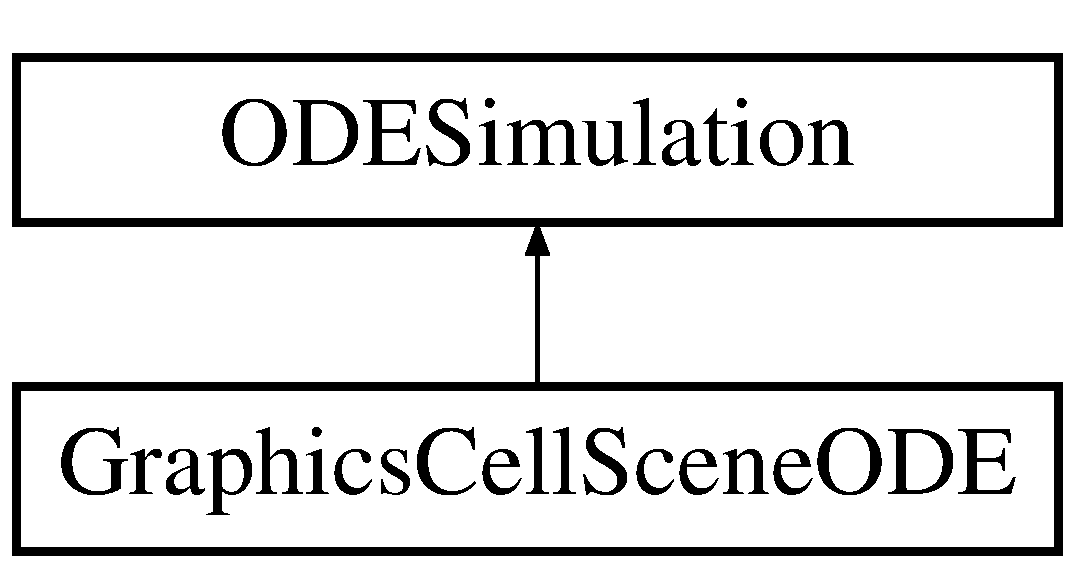
\includegraphics[height=2.000000cm]{class_graphics_cell_scene_o_d_e}
\end{center}
\end{figure}
\subsection*{\-Public \-Member \-Functions}
\begin{DoxyCompactItemize}
\item 
\hyperlink{class_graphics_cell_scene_o_d_e_a4b93b6c25c3199a42f9464cae8a0cdc6}{\-Graphics\-Cell\-Scene\-O\-D\-E} (\-Q\-Object $\ast$parent=0)
\item 
void \hyperlink{class_graphics_cell_scene_o_d_e_ac2d1365626ed2d7492c8a78e0098efd5}{set\-Cell\-Position} (int cell\-Index, double x, double y)
\item 
virtual \-Graphics\-Cell $\ast$ \hyperlink{class_graphics_cell_scene_o_d_e_a77f0a529438123786cca3050eec57719}{add\-One\-Cell} (int cell\-Index)
\item 
virtual void \hyperlink{class_graphics_cell_scene_o_d_e_ae66f4605023f6b82360b2ade0496d098}{duplicate\-Cell} (int mother\-Cell\-Index)
\item 
virtual void \hyperlink{class_graphics_cell_scene_o_d_e_a1d7fdc85e9cba222a530e473751aed21}{delete\-One\-Cell} (int cell\-Index)
\item 
void \hyperlink{class_graphics_cell_scene_o_d_e_ade7cd7d3f3c55a2a474d80eb63736698}{compute\-O\-D\-E\-Step} (float time\-Step, bool equilibration)
\item 
\-Graphics\-Wall $\ast$ \hyperlink{class_graphics_cell_scene_o_d_e_aea5ea730a60d9f141623e2f39a8d599f}{add\-Wall} (float center\-X, float center\-Y, float normal\-X, float normal\-Y, float thickness, float length)
\end{DoxyCompactItemize}


\subsection{\-Detailed \-Description}
\-Graphics scene of the cell colony in the \-Qt \-Graphics framework with \-Open \-Dynamics \-Engine (\-O\-D\-E) simulation. \-Derives from \-Graphics\-Cell\-Scene, \hyperlink{class_o_d_e_simulation}{\-O\-D\-E\-Simulation}. 

\-Definition at line 33 of file \-Graphics\-Cell\-Scene\-O\-D\-E.\-h.



\subsection{\-Constructor \& \-Destructor \-Documentation}
\hypertarget{class_graphics_cell_scene_o_d_e_a4b93b6c25c3199a42f9464cae8a0cdc6}{\index{\-Graphics\-Cell\-Scene\-O\-D\-E@{\-Graphics\-Cell\-Scene\-O\-D\-E}!\-Graphics\-Cell\-Scene\-O\-D\-E@{\-Graphics\-Cell\-Scene\-O\-D\-E}}
\index{\-Graphics\-Cell\-Scene\-O\-D\-E@{\-Graphics\-Cell\-Scene\-O\-D\-E}!GraphicsCellSceneODE@{\-Graphics\-Cell\-Scene\-O\-D\-E}}
\subsubsection[{\-Graphics\-Cell\-Scene\-O\-D\-E}]{\setlength{\rightskip}{0pt plus 5cm}{\bf \-Graphics\-Cell\-Scene\-O\-D\-E\-::\-Graphics\-Cell\-Scene\-O\-D\-E} (
\begin{DoxyParamCaption}
\item[{\-Q\-Object $\ast$}]{parent = {\ttfamily 0}}
\end{DoxyParamCaption}
)}}\label{class_graphics_cell_scene_o_d_e_a4b93b6c25c3199a42f9464cae8a0cdc6}


\-Definition at line 20 of file \-Graphics\-Cell\-Scene\-O\-D\-E.\-cpp.



\subsection{\-Member \-Function \-Documentation}
\hypertarget{class_graphics_cell_scene_o_d_e_a77f0a529438123786cca3050eec57719}{\index{\-Graphics\-Cell\-Scene\-O\-D\-E@{\-Graphics\-Cell\-Scene\-O\-D\-E}!add\-One\-Cell@{add\-One\-Cell}}
\index{add\-One\-Cell@{add\-One\-Cell}!GraphicsCellSceneODE@{\-Graphics\-Cell\-Scene\-O\-D\-E}}
\subsubsection[{add\-One\-Cell}]{\setlength{\rightskip}{0pt plus 5cm}\-Graphics\-Cell $\ast$ {\bf \-Graphics\-Cell\-Scene\-O\-D\-E\-::add\-One\-Cell} (
\begin{DoxyParamCaption}
\item[{int}]{cell\-Index}
\end{DoxyParamCaption}
)\hspace{0.3cm}{\ttfamily  \mbox{[}virtual\mbox{]}}}}\label{class_graphics_cell_scene_o_d_e_a77f0a529438123786cca3050eec57719}
\-Add a new cell to the colony scene. 

\-Definition at line 64 of file \-Graphics\-Cell\-Scene\-O\-D\-E.\-cpp.

\hypertarget{class_graphics_cell_scene_o_d_e_aea5ea730a60d9f141623e2f39a8d599f}{\index{\-Graphics\-Cell\-Scene\-O\-D\-E@{\-Graphics\-Cell\-Scene\-O\-D\-E}!add\-Wall@{add\-Wall}}
\index{add\-Wall@{add\-Wall}!GraphicsCellSceneODE@{\-Graphics\-Cell\-Scene\-O\-D\-E}}
\subsubsection[{add\-Wall}]{\setlength{\rightskip}{0pt plus 5cm}\-Graphics\-Wall $\ast$ {\bf \-Graphics\-Cell\-Scene\-O\-D\-E\-::add\-Wall} (
\begin{DoxyParamCaption}
\item[{float}]{center\-X, }
\item[{float}]{center\-Y, }
\item[{float}]{normal\-X, }
\item[{float}]{normal\-Y, }
\item[{float}]{thickness, }
\item[{float}]{length}
\end{DoxyParamCaption}
)}}\label{class_graphics_cell_scene_o_d_e_aea5ea730a60d9f141623e2f39a8d599f}


\-Definition at line 27 of file \-Graphics\-Cell\-Scene\-O\-D\-E.\-cpp.

\hypertarget{class_graphics_cell_scene_o_d_e_ade7cd7d3f3c55a2a474d80eb63736698}{\index{\-Graphics\-Cell\-Scene\-O\-D\-E@{\-Graphics\-Cell\-Scene\-O\-D\-E}!compute\-O\-D\-E\-Step@{compute\-O\-D\-E\-Step}}
\index{compute\-O\-D\-E\-Step@{compute\-O\-D\-E\-Step}!GraphicsCellSceneODE@{\-Graphics\-Cell\-Scene\-O\-D\-E}}
\subsubsection[{compute\-O\-D\-E\-Step}]{\setlength{\rightskip}{0pt plus 5cm}void {\bf \-Graphics\-Cell\-Scene\-O\-D\-E\-::compute\-O\-D\-E\-Step} (
\begin{DoxyParamCaption}
\item[{float}]{time\-Step, }
\item[{bool}]{equilibration}
\end{DoxyParamCaption}
)}}\label{class_graphics_cell_scene_o_d_e_ade7cd7d3f3c55a2a474d80eb63736698}
\-Compute timestep of the \-O\-D\-E simulation. 
\begin{DoxyItemize}
\item \-Compute the \-O\-D\-E step.
\end{DoxyItemize}


\begin{DoxyItemize}
\item \-Send the cell positions and angle to the simulation/\-Cell\-Collection object. 
\end{DoxyItemize}

\-Definition at line 117 of file \-Graphics\-Cell\-Scene\-O\-D\-E.\-cpp.

\hypertarget{class_graphics_cell_scene_o_d_e_a1d7fdc85e9cba222a530e473751aed21}{\index{\-Graphics\-Cell\-Scene\-O\-D\-E@{\-Graphics\-Cell\-Scene\-O\-D\-E}!delete\-One\-Cell@{delete\-One\-Cell}}
\index{delete\-One\-Cell@{delete\-One\-Cell}!GraphicsCellSceneODE@{\-Graphics\-Cell\-Scene\-O\-D\-E}}
\subsubsection[{delete\-One\-Cell}]{\setlength{\rightskip}{0pt plus 5cm}void {\bf \-Graphics\-Cell\-Scene\-O\-D\-E\-::delete\-One\-Cell} (
\begin{DoxyParamCaption}
\item[{int}]{cell\-Index}
\end{DoxyParamCaption}
)\hspace{0.3cm}{\ttfamily  \mbox{[}virtual\mbox{]}}}}\label{class_graphics_cell_scene_o_d_e_a1d7fdc85e9cba222a530e473751aed21}


\-Definition at line 93 of file \-Graphics\-Cell\-Scene\-O\-D\-E.\-cpp.

\hypertarget{class_graphics_cell_scene_o_d_e_ae66f4605023f6b82360b2ade0496d098}{\index{\-Graphics\-Cell\-Scene\-O\-D\-E@{\-Graphics\-Cell\-Scene\-O\-D\-E}!duplicate\-Cell@{duplicate\-Cell}}
\index{duplicate\-Cell@{duplicate\-Cell}!GraphicsCellSceneODE@{\-Graphics\-Cell\-Scene\-O\-D\-E}}
\subsubsection[{duplicate\-Cell}]{\setlength{\rightskip}{0pt plus 5cm}void {\bf \-Graphics\-Cell\-Scene\-O\-D\-E\-::duplicate\-Cell} (
\begin{DoxyParamCaption}
\item[{int}]{mother\-Cell\-Index}
\end{DoxyParamCaption}
)\hspace{0.3cm}{\ttfamily  \mbox{[}virtual\mbox{]}}}}\label{class_graphics_cell_scene_o_d_e_ae66f4605023f6b82360b2ade0496d098}
\-Duplicate cell. 

\-Definition at line 74 of file \-Graphics\-Cell\-Scene\-O\-D\-E.\-cpp.

\hypertarget{class_graphics_cell_scene_o_d_e_ac2d1365626ed2d7492c8a78e0098efd5}{\index{\-Graphics\-Cell\-Scene\-O\-D\-E@{\-Graphics\-Cell\-Scene\-O\-D\-E}!set\-Cell\-Position@{set\-Cell\-Position}}
\index{set\-Cell\-Position@{set\-Cell\-Position}!GraphicsCellSceneODE@{\-Graphics\-Cell\-Scene\-O\-D\-E}}
\subsubsection[{set\-Cell\-Position}]{\setlength{\rightskip}{0pt plus 5cm}void {\bf \-Graphics\-Cell\-Scene\-O\-D\-E\-::set\-Cell\-Position} (
\begin{DoxyParamCaption}
\item[{int}]{cell\-Index, }
\item[{double}]{x, }
\item[{double}]{y}
\end{DoxyParamCaption}
)}}\label{class_graphics_cell_scene_o_d_e_ac2d1365626ed2d7492c8a78e0098efd5}
\-Set the position of cell with index cell\-Index. \hyperlink{class_input}{\-Input} coordinates are in the simulation coordinates system with range \mbox{[}0,1\mbox{]} and conversion to \-Graphics coordinate is automatically done. 

\-Definition at line 51 of file \-Graphics\-Cell\-Scene\-O\-D\-E.\-cpp.



\-The documentation for this class was generated from the following files\-:\begin{DoxyCompactItemize}
\item 
/media/\-My\-Passport\-Blue/\-Data/\-Research/\-Simulations/\-Colony/\hyperlink{_graphics_cell_scene_o_d_e_8h}{\-Graphics\-Cell\-Scene\-O\-D\-E.\-h}\item 
/media/\-My\-Passport\-Blue/\-Data/\-Research/\-Simulations/\-Colony/\hyperlink{_graphics_cell_scene_o_d_e_8cpp}{\-Graphics\-Cell\-Scene\-O\-D\-E.\-cpp}\end{DoxyCompactItemize}

\hypertarget{class_input}{\section{\-Input \-Class \-Reference}
\label{class_input}\index{\-Input@{\-Input}}
}


{\ttfamily \#include $<$\-Input.\-h$>$}

\subsection*{\-Public \-Member \-Functions}
\begin{DoxyCompactItemize}
\item 
\hyperlink{class_input_afa58ad9bb35043a7f1695b050fc8883d}{\-Input} (string input\-File)
\item 
\hyperlink{class_input_af2db35ba67c8a8ccd23bef6a482fc291}{$\sim$\-Input} ()
\item 
void \hyperlink{class_input_aa208108461c7017b929db50cec33175d}{set\-Global\-Parameter} (const double time)
\item 
void \hyperlink{class_input_a8f085cfd1e929ffeb6493d52265f69d9}{set\-Index\-Parameter\-Set} (const int i)
\item 
int \hyperlink{class_input_aabbb875892aef9fb2e3855f85f742c85}{get\-N\-Parameter\-Set} () const 
\item 
void \hyperlink{class_input_a91e616b5ca9b6abd2a6cda642b3b1376}{set\-X0} (const int i\-Parameter\-Set)
\end{DoxyCompactItemize}
\subsection*{\-Public \-Attributes}
\begin{DoxyCompactItemize}
\item 
int \hyperlink{class_input_a9ba0dddeba07d5be04e894c6ceecd6d9}{seed}
\item 
\-Cell\-Collection\-Param \hyperlink{class_input_a2d15599a9c23b27330ae868928d2997d}{p}
\item 
\-Simulator\-Param \hyperlink{class_input_acc3f4f428e3a7e40eec817496ad85deb}{sim}
\item 
\-Output\-Param \hyperlink{class_input_a4efa8e11da83057d1a7a7b828033438d}{out}
\end{DoxyCompactItemize}
\subsection*{\-Static \-Public \-Attributes}
\begin{DoxyCompactItemize}
\item 
static double \hyperlink{class_input_ad9902e799cfa4f3b81a9693448ae113f}{\-O\-D\-E\-Equilibration\-Time}
\item 
static \-Array$<$ double, 1 $>$ \hyperlink{class_input_a7d05df10573a8036c8a403b2d4c73ac9}{global\-Parameter}
\item 
static \-Array$<$ double, 3 $>$ \hyperlink{class_input_a86be833bf32a0e6e5deec8da213e7e6f}{global\-Parameter\-Time\-Points}
\item 
static vector$<$ string $>$ \hyperlink{class_input_ab6ad759b315761a306fd95353b31c1a4}{list\-Global\-Parameters\-Name}
\end{DoxyCompactItemize}


\subsection{\-Detailed \-Description}
\-Input parameters read from files \char`\"{}input.\-dat\char`\"{} and \char`\"{}input\-\_\-simulation.\-dat\char`\"{} in executable's directory. 

\-Definition at line 63 of file \-Input.\-h.



\subsection{\-Constructor \& \-Destructor \-Documentation}
\hypertarget{class_input_afa58ad9bb35043a7f1695b050fc8883d}{\index{\-Input@{\-Input}!\-Input@{\-Input}}
\index{\-Input@{\-Input}!Input@{\-Input}}
\subsubsection[{\-Input}]{\setlength{\rightskip}{0pt plus 5cm}{\bf \-Input\-::\-Input} (
\begin{DoxyParamCaption}
\item[{string}]{input\-File}
\end{DoxyParamCaption}
)}}\label{class_input_afa58ad9bb35043a7f1695b050fc8883d}
\-The default constructor reads the input from file \char`\"{}input.\-dat\char`\"{} and \char`\"{}input\-\_\-simulation.\-dat\char`\"{} 

\-Definition at line 30 of file \-Input.\-cpp.

\hypertarget{class_input_af2db35ba67c8a8ccd23bef6a482fc291}{\index{\-Input@{\-Input}!$\sim$\-Input@{$\sim$\-Input}}
\index{$\sim$\-Input@{$\sim$\-Input}!Input@{\-Input}}
\subsubsection[{$\sim$\-Input}]{\setlength{\rightskip}{0pt plus 5cm}{\bf \-Input\-::$\sim$\-Input} (
\begin{DoxyParamCaption}
{}
\end{DoxyParamCaption}
)}}\label{class_input_af2db35ba67c8a8ccd23bef6a482fc291}


\-Definition at line 345 of file \-Input.\-cpp.



\subsection{\-Member \-Function \-Documentation}
\hypertarget{class_input_aabbb875892aef9fb2e3855f85f742c85}{\index{\-Input@{\-Input}!get\-N\-Parameter\-Set@{get\-N\-Parameter\-Set}}
\index{get\-N\-Parameter\-Set@{get\-N\-Parameter\-Set}!Input@{\-Input}}
\subsubsection[{get\-N\-Parameter\-Set}]{\setlength{\rightskip}{0pt plus 5cm}int {\bf \-Input\-::get\-N\-Parameter\-Set} (
\begin{DoxyParamCaption}
{}
\end{DoxyParamCaption}
) const}}\label{class_input_aabbb875892aef9fb2e3855f85f742c85}


\-Definition at line 398 of file \-Input.\-cpp.

\hypertarget{class_input_aa208108461c7017b929db50cec33175d}{\index{\-Input@{\-Input}!set\-Global\-Parameter@{set\-Global\-Parameter}}
\index{set\-Global\-Parameter@{set\-Global\-Parameter}!Input@{\-Input}}
\subsubsection[{set\-Global\-Parameter}]{\setlength{\rightskip}{0pt plus 5cm}void {\bf \-Input\-::set\-Global\-Parameter} (
\begin{DoxyParamCaption}
\item[{const double}]{time}
\end{DoxyParamCaption}
)}}\label{class_input_aa208108461c7017b929db50cec33175d}


\-Definition at line 350 of file \-Input.\-cpp.

\hypertarget{class_input_a8f085cfd1e929ffeb6493d52265f69d9}{\index{\-Input@{\-Input}!set\-Index\-Parameter\-Set@{set\-Index\-Parameter\-Set}}
\index{set\-Index\-Parameter\-Set@{set\-Index\-Parameter\-Set}!Input@{\-Input}}
\subsubsection[{set\-Index\-Parameter\-Set}]{\setlength{\rightskip}{0pt plus 5cm}void {\bf \-Input\-::set\-Index\-Parameter\-Set} (
\begin{DoxyParamCaption}
\item[{const int}]{i}
\end{DoxyParamCaption}
)}}\label{class_input_a8f085cfd1e929ffeb6493d52265f69d9}


\-Definition at line 391 of file \-Input.\-cpp.

\hypertarget{class_input_a91e616b5ca9b6abd2a6cda642b3b1376}{\index{\-Input@{\-Input}!set\-X0@{set\-X0}}
\index{set\-X0@{set\-X0}!Input@{\-Input}}
\subsubsection[{set\-X0}]{\setlength{\rightskip}{0pt plus 5cm}void {\bf \-Input\-::set\-X0} (
\begin{DoxyParamCaption}
\item[{const int}]{i\-Parameter\-Set}
\end{DoxyParamCaption}
)}}\label{class_input_a91e616b5ca9b6abd2a6cda642b3b1376}


\-Definition at line 363 of file \-Input.\-cpp.



\subsection{\-Member \-Data \-Documentation}
\hypertarget{class_input_a7d05df10573a8036c8a403b2d4c73ac9}{\index{\-Input@{\-Input}!global\-Parameter@{global\-Parameter}}
\index{global\-Parameter@{global\-Parameter}!Input@{\-Input}}
\subsubsection[{global\-Parameter}]{\setlength{\rightskip}{0pt plus 5cm}\-Array$<$ double, 1 $>$ {\bf \-Input\-::global\-Parameter}\hspace{0.3cm}{\ttfamily  \mbox{[}static\mbox{]}}}}\label{class_input_a7d05df10573a8036c8a403b2d4c73ac9}


\-Definition at line 97 of file \-Input.\-h.

\hypertarget{class_input_a86be833bf32a0e6e5deec8da213e7e6f}{\index{\-Input@{\-Input}!global\-Parameter\-Time\-Points@{global\-Parameter\-Time\-Points}}
\index{global\-Parameter\-Time\-Points@{global\-Parameter\-Time\-Points}!Input@{\-Input}}
\subsubsection[{global\-Parameter\-Time\-Points}]{\setlength{\rightskip}{0pt plus 5cm}\-Array$<$ double, 3 $>$ {\bf \-Input\-::global\-Parameter\-Time\-Points}\hspace{0.3cm}{\ttfamily  \mbox{[}static\mbox{]}}}}\label{class_input_a86be833bf32a0e6e5deec8da213e7e6f}


\-Definition at line 99 of file \-Input.\-h.

\hypertarget{class_input_ab6ad759b315761a306fd95353b31c1a4}{\index{\-Input@{\-Input}!list\-Global\-Parameters\-Name@{list\-Global\-Parameters\-Name}}
\index{list\-Global\-Parameters\-Name@{list\-Global\-Parameters\-Name}!Input@{\-Input}}
\subsubsection[{list\-Global\-Parameters\-Name}]{\setlength{\rightskip}{0pt plus 5cm}vector$<$ string $>$ {\bf \-Input\-::list\-Global\-Parameters\-Name}\hspace{0.3cm}{\ttfamily  \mbox{[}static\mbox{]}}}}\label{class_input_ab6ad759b315761a306fd95353b31c1a4}


\-Definition at line 101 of file \-Input.\-h.

\hypertarget{class_input_ad9902e799cfa4f3b81a9693448ae113f}{\index{\-Input@{\-Input}!\-O\-D\-E\-Equilibration\-Time@{\-O\-D\-E\-Equilibration\-Time}}
\index{\-O\-D\-E\-Equilibration\-Time@{\-O\-D\-E\-Equilibration\-Time}!Input@{\-Input}}
\subsubsection[{\-O\-D\-E\-Equilibration\-Time}]{\setlength{\rightskip}{0pt plus 5cm}double {\bf \-Input\-::\-O\-D\-E\-Equilibration\-Time}\hspace{0.3cm}{\ttfamily  \mbox{[}static\mbox{]}}}}\label{class_input_ad9902e799cfa4f3b81a9693448ae113f}


\-Definition at line 89 of file \-Input.\-h.

\hypertarget{class_input_a4efa8e11da83057d1a7a7b828033438d}{\index{\-Input@{\-Input}!out@{out}}
\index{out@{out}!Input@{\-Input}}
\subsubsection[{out}]{\setlength{\rightskip}{0pt plus 5cm}\-Output\-Param {\bf \-Input\-::out}}}\label{class_input_a4efa8e11da83057d1a7a7b828033438d}


\-Definition at line 95 of file \-Input.\-h.

\hypertarget{class_input_a2d15599a9c23b27330ae868928d2997d}{\index{\-Input@{\-Input}!p@{p}}
\index{p@{p}!Input@{\-Input}}
\subsubsection[{p}]{\setlength{\rightskip}{0pt plus 5cm}\-Cell\-Collection\-Param {\bf \-Input\-::p}}}\label{class_input_a2d15599a9c23b27330ae868928d2997d}


\-Definition at line 91 of file \-Input.\-h.

\hypertarget{class_input_a9ba0dddeba07d5be04e894c6ceecd6d9}{\index{\-Input@{\-Input}!seed@{seed}}
\index{seed@{seed}!Input@{\-Input}}
\subsubsection[{seed}]{\setlength{\rightskip}{0pt plus 5cm}int {\bf \-Input\-::seed}}}\label{class_input_a9ba0dddeba07d5be04e894c6ceecd6d9}


\-Definition at line 87 of file \-Input.\-h.

\hypertarget{class_input_acc3f4f428e3a7e40eec817496ad85deb}{\index{\-Input@{\-Input}!sim@{sim}}
\index{sim@{sim}!Input@{\-Input}}
\subsubsection[{sim}]{\setlength{\rightskip}{0pt plus 5cm}\-Simulator\-Param {\bf \-Input\-::sim}}}\label{class_input_acc3f4f428e3a7e40eec817496ad85deb}


\-Definition at line 93 of file \-Input.\-h.



\-The documentation for this class was generated from the following files\-:\begin{DoxyCompactItemize}
\item 
/media/\-My\-Passport\-Blue/\-Data/\-Research/\-Simulations/\-Colony/\hyperlink{_input_8h}{\-Input.\-h}\item 
/media/\-My\-Passport\-Blue/\-Data/\-Research/\-Simulations/\-Colony/\hyperlink{_input_8cpp}{\-Input.\-cpp}\end{DoxyCompactItemize}

\hypertarget{class_integrator_chemical_langevin}{\section{\-Integrator\-Chemical\-Langevin \-Class \-Reference}
\label{class_integrator_chemical_langevin}\index{\-Integrator\-Chemical\-Langevin@{\-Integrator\-Chemical\-Langevin}}
}


{\ttfamily \#include $<$\-Integrator\-Chemical\-Langevin.\-h$>$}

\subsection*{\-Public \-Member \-Functions}
\begin{DoxyCompactItemize}
\item 
\hyperlink{class_integrator_chemical_langevin_ab71a74a8bc87d8ae7a12b75d00b8010e}{\-Integrator\-Chemical\-Langevin} (\hyperlink{class_simulator}{\-Simulator} $\ast$simulator\-Ptr)
\item 
\hyperlink{class_integrator_chemical_langevin_ad3da14ad4ab5d2cc6d7498839d977a26}{$\sim$\-Integrator\-Chemical\-Langevin} ()
\item 
void \hyperlink{class_integrator_chemical_langevin_ac7c751bb531f9923149d38316a7d48fd}{integrate\-One\-Step} ()
\item 
void \hyperlink{class_integrator_chemical_langevin_a453c4de6202e63b107cc093566bcfe73}{integrate\-One\-Step} (double time\-Step)
\item 
void \hyperlink{class_integrator_chemical_langevin_a8d780c68e33d062628b848236cf52a59}{set\-Fixed\-N\-Cells} (int n\-Cells)
\end{DoxyCompactItemize}


\subsection{\-Detailed \-Description}
\-Algorithm of \-Euler for the chemical \-Langevin equation. 

\-Definition at line 53 of file \-Integrator\-Chemical\-Langevin.\-h.



\subsection{\-Constructor \& \-Destructor \-Documentation}
\hypertarget{class_integrator_chemical_langevin_ab71a74a8bc87d8ae7a12b75d00b8010e}{\index{\-Integrator\-Chemical\-Langevin@{\-Integrator\-Chemical\-Langevin}!\-Integrator\-Chemical\-Langevin@{\-Integrator\-Chemical\-Langevin}}
\index{\-Integrator\-Chemical\-Langevin@{\-Integrator\-Chemical\-Langevin}!IntegratorChemicalLangevin@{\-Integrator\-Chemical\-Langevin}}
\subsubsection[{\-Integrator\-Chemical\-Langevin}]{\setlength{\rightskip}{0pt plus 5cm}{\bf \-Integrator\-Chemical\-Langevin\-::\-Integrator\-Chemical\-Langevin} (
\begin{DoxyParamCaption}
\item[{{\bf \-Simulator} $\ast$}]{simulator\-Ptr}
\end{DoxyParamCaption}
)}}\label{class_integrator_chemical_langevin_ab71a74a8bc87d8ae7a12b75d00b8010e}
\-Initiate the \hyperlink{class_integrator_context}{\-Integrator\-Context} with the pointer to the \hyperlink{class_simulator}{\-Simulator} object as argument. \hypertarget{class_integrator_chemical_langevin_ad3da14ad4ab5d2cc6d7498839d977a26}{\index{\-Integrator\-Chemical\-Langevin@{\-Integrator\-Chemical\-Langevin}!$\sim$\-Integrator\-Chemical\-Langevin@{$\sim$\-Integrator\-Chemical\-Langevin}}
\index{$\sim$\-Integrator\-Chemical\-Langevin@{$\sim$\-Integrator\-Chemical\-Langevin}!IntegratorChemicalLangevin@{\-Integrator\-Chemical\-Langevin}}
\subsubsection[{$\sim$\-Integrator\-Chemical\-Langevin}]{\setlength{\rightskip}{0pt plus 5cm}{\bf \-Integrator\-Chemical\-Langevin\-::$\sim$\-Integrator\-Chemical\-Langevin} (
\begin{DoxyParamCaption}
{}
\end{DoxyParamCaption}
)}}\label{class_integrator_chemical_langevin_ad3da14ad4ab5d2cc6d7498839d977a26}


\subsection{\-Member \-Function \-Documentation}
\hypertarget{class_integrator_chemical_langevin_ac7c751bb531f9923149d38316a7d48fd}{\index{\-Integrator\-Chemical\-Langevin@{\-Integrator\-Chemical\-Langevin}!integrate\-One\-Step@{integrate\-One\-Step}}
\index{integrate\-One\-Step@{integrate\-One\-Step}!IntegratorChemicalLangevin@{\-Integrator\-Chemical\-Langevin}}
\subsubsection[{integrate\-One\-Step}]{\setlength{\rightskip}{0pt plus 5cm}void {\bf \-Integrator\-Chemical\-Langevin\-::integrate\-One\-Step} (
\begin{DoxyParamCaption}
{}
\end{DoxyParamCaption}
)\hspace{0.3cm}{\ttfamily  \mbox{[}inline\mbox{]}}}}\label{class_integrator_chemical_langevin_ac7c751bb531f9923149d38316a7d48fd}
\-This method is not used in this integrator class. 

\-Definition at line 68 of file \-Integrator\-Chemical\-Langevin.\-h.

\hypertarget{class_integrator_chemical_langevin_a453c4de6202e63b107cc093566bcfe73}{\index{\-Integrator\-Chemical\-Langevin@{\-Integrator\-Chemical\-Langevin}!integrate\-One\-Step@{integrate\-One\-Step}}
\index{integrate\-One\-Step@{integrate\-One\-Step}!IntegratorChemicalLangevin@{\-Integrator\-Chemical\-Langevin}}
\subsubsection[{integrate\-One\-Step}]{\setlength{\rightskip}{0pt plus 5cm}void {\bf \-Integrator\-Chemical\-Langevin\-::integrate\-One\-Step} (
\begin{DoxyParamCaption}
\item[{double}]{time\-Step}
\end{DoxyParamCaption}
)}}\label{class_integrator_chemical_langevin_a453c4de6202e63b107cc093566bcfe73}
\-Integrate one step in the chemical \-Langevin algorithm. \hypertarget{class_integrator_chemical_langevin_a8d780c68e33d062628b848236cf52a59}{\index{\-Integrator\-Chemical\-Langevin@{\-Integrator\-Chemical\-Langevin}!set\-Fixed\-N\-Cells@{set\-Fixed\-N\-Cells}}
\index{set\-Fixed\-N\-Cells@{set\-Fixed\-N\-Cells}!IntegratorChemicalLangevin@{\-Integrator\-Chemical\-Langevin}}
\subsubsection[{set\-Fixed\-N\-Cells}]{\setlength{\rightskip}{0pt plus 5cm}void {\bf \-Integrator\-Chemical\-Langevin\-::set\-Fixed\-N\-Cells} (
\begin{DoxyParamCaption}
\item[{int}]{n\-Cells}
\end{DoxyParamCaption}
)\hspace{0.3cm}{\ttfamily  \mbox{[}inline\mbox{]}}}}\label{class_integrator_chemical_langevin_a8d780c68e33d062628b848236cf52a59}


\-Definition at line 76 of file \-Integrator\-Chemical\-Langevin.\-h.



\-The documentation for this class was generated from the following file\-:\begin{DoxyCompactItemize}
\item 
/media/\-My\-Passport\-Blue/\-Data/\-Research/\-Simulations/\-Colony/\hyperlink{_integrator_chemical_langevin_8h}{\-Integrator\-Chemical\-Langevin.\-h}\end{DoxyCompactItemize}

\hypertarget{class_integrator_context}{\section{\-Integrator\-Context$<$ \-Integrator\-Type $>$ \-Class \-Template \-Reference}
\label{class_integrator_context}\index{\-Integrator\-Context$<$ Integrator\-Type $>$@{\-Integrator\-Context$<$ Integrator\-Type $>$}}
}


{\ttfamily \#include $<$\-Integrator\-Context.\-h$>$}

\subsection*{\-Public \-Member \-Functions}
\begin{DoxyCompactItemize}
\item 
\hyperlink{class_integrator_context_a020c17d49d7cee23c24a850213c75d15}{\-Integrator\-Context} (\hyperlink{class_simulator}{\-Simulator} $\ast$simulator\-Ptr)
\item 
\hyperlink{class_integrator_context_a0c2a801de04ed8799d51448cc68ef513}{$\sim$\-Integrator\-Context} ()
\item 
void \hyperlink{class_integrator_context_a72b6def867485fd2710fb55b4602194e}{integrate\-One\-Step} ()
\item 
void \hyperlink{class_integrator_context_ac2e7c5186de42a0cf400277f72942966}{integrate\-One\-Step} (double time\-Step)
\end{DoxyCompactItemize}
\subsection*{\-Public \-Attributes}
\begin{DoxyCompactItemize}
\item 
\-Integrator\-Type \hyperlink{class_integrator_context_a16de83daa9438581f2c1c42540bb9299}{integrator\-\_\-}
\end{DoxyCompactItemize}


\subsection{\-Detailed \-Description}
\subsubsection*{template$<$class \-Integrator\-Type$>$class Integrator\-Context$<$ Integrator\-Type $>$}

\-Template class that defines the context for the integrator. \-The \hyperlink{class_integrator_context}{\-Integrator\-Context} class is a template class with template type defining the type of integrator (\-Gillespie, modified \-Gillespie, etc). \-It contains an \-Integrator\-Type object and uses its \hyperlink{class_integrator_context_a72b6def867485fd2710fb55b4602194e}{integrate\-One\-Step()} function. 

\-Definition at line 50 of file \-Integrator\-Context.\-h.



\subsection{\-Constructor \& \-Destructor \-Documentation}
\hypertarget{class_integrator_context_a020c17d49d7cee23c24a850213c75d15}{\index{\-Integrator\-Context@{\-Integrator\-Context}!\-Integrator\-Context@{\-Integrator\-Context}}
\index{\-Integrator\-Context@{\-Integrator\-Context}!IntegratorContext@{\-Integrator\-Context}}
\subsubsection[{\-Integrator\-Context}]{\setlength{\rightskip}{0pt plus 5cm}template$<$class Integrator\-Type $>$ {\bf \-Integrator\-Context}$<$ \-Integrator\-Type $>$\-::{\bf \-Integrator\-Context} (
\begin{DoxyParamCaption}
\item[{{\bf \-Simulator} $\ast$}]{simulator\-Ptr}
\end{DoxyParamCaption}
)}}\label{class_integrator_context_a020c17d49d7cee23c24a850213c75d15}
\-Initiate the \hyperlink{class_integrator_context}{\-Integrator\-Context} with the pointer to the \hyperlink{class_simulator}{\-Simulator} object as argument. 

\-Definition at line 21 of file \-Integrator\-Context.\-cpp.

\hypertarget{class_integrator_context_a0c2a801de04ed8799d51448cc68ef513}{\index{\-Integrator\-Context@{\-Integrator\-Context}!$\sim$\-Integrator\-Context@{$\sim$\-Integrator\-Context}}
\index{$\sim$\-Integrator\-Context@{$\sim$\-Integrator\-Context}!IntegratorContext@{\-Integrator\-Context}}
\subsubsection[{$\sim$\-Integrator\-Context}]{\setlength{\rightskip}{0pt plus 5cm}template$<$class Integrator\-Type $>$ {\bf \-Integrator\-Context}$<$ \-Integrator\-Type $>$\-::$\sim${\bf \-Integrator\-Context} (
\begin{DoxyParamCaption}
{}
\end{DoxyParamCaption}
)}}\label{class_integrator_context_a0c2a801de04ed8799d51448cc68ef513}


\-Definition at line 28 of file \-Integrator\-Context.\-cpp.



\subsection{\-Member \-Function \-Documentation}
\hypertarget{class_integrator_context_a72b6def867485fd2710fb55b4602194e}{\index{\-Integrator\-Context@{\-Integrator\-Context}!integrate\-One\-Step@{integrate\-One\-Step}}
\index{integrate\-One\-Step@{integrate\-One\-Step}!IntegratorContext@{\-Integrator\-Context}}
\subsubsection[{integrate\-One\-Step}]{\setlength{\rightskip}{0pt plus 5cm}template$<$class \-Integrator\-Type$>$ void {\bf \-Integrator\-Context}$<$ \-Integrator\-Type $>$\-::{\bf integrate\-One\-Step} (
\begin{DoxyParamCaption}
{}
\end{DoxyParamCaption}
)\hspace{0.3cm}{\ttfamily  \mbox{[}inline\mbox{]}}}}\label{class_integrator_context_a72b6def867485fd2710fb55b4602194e}


\-Definition at line 63 of file \-Integrator\-Context.\-h.

\hypertarget{class_integrator_context_ac2e7c5186de42a0cf400277f72942966}{\index{\-Integrator\-Context@{\-Integrator\-Context}!integrate\-One\-Step@{integrate\-One\-Step}}
\index{integrate\-One\-Step@{integrate\-One\-Step}!IntegratorContext@{\-Integrator\-Context}}
\subsubsection[{integrate\-One\-Step}]{\setlength{\rightskip}{0pt plus 5cm}template$<$class \-Integrator\-Type$>$ void {\bf \-Integrator\-Context}$<$ \-Integrator\-Type $>$\-::{\bf integrate\-One\-Step} (
\begin{DoxyParamCaption}
\item[{double}]{time\-Step}
\end{DoxyParamCaption}
)\hspace{0.3cm}{\ttfamily  \mbox{[}inline\mbox{]}}}}\label{class_integrator_context_ac2e7c5186de42a0cf400277f72942966}


\-Definition at line 68 of file \-Integrator\-Context.\-h.



\subsection{\-Member \-Data \-Documentation}
\hypertarget{class_integrator_context_a16de83daa9438581f2c1c42540bb9299}{\index{\-Integrator\-Context@{\-Integrator\-Context}!integrator\-\_\-@{integrator\-\_\-}}
\index{integrator\-\_\-@{integrator\-\_\-}!IntegratorContext@{\-Integrator\-Context}}
\subsubsection[{integrator\-\_\-}]{\setlength{\rightskip}{0pt plus 5cm}template$<$class \-Integrator\-Type$>$ \-Integrator\-Type {\bf \-Integrator\-Context}$<$ \-Integrator\-Type $>$\-::{\bf integrator\-\_\-}}}\label{class_integrator_context_a16de83daa9438581f2c1c42540bb9299}


\-Definition at line 73 of file \-Integrator\-Context.\-h.



\-The documentation for this class was generated from the following files\-:\begin{DoxyCompactItemize}
\item 
/media/\-My\-Passport\-Blue/\-Data/\-Research/\-Simulations/\-Colony/\hyperlink{_integrator_context_8h}{\-Integrator\-Context.\-h}\item 
/media/\-My\-Passport\-Blue/\-Data/\-Research/\-Simulations/\-Colony/\hyperlink{_integrator_context_8cpp}{\-Integrator\-Context.\-cpp}\end{DoxyCompactItemize}

\hypertarget{class_integrator_gillespie}{\section{\-Integrator\-Gillespie \-Class \-Reference}
\label{class_integrator_gillespie}\index{\-Integrator\-Gillespie@{\-Integrator\-Gillespie}}
}


{\ttfamily \#include $<$\-Integrator\-Gillespie.\-h$>$}

\subsection*{\-Public \-Member \-Functions}
\begin{DoxyCompactItemize}
\item 
\hyperlink{class_integrator_gillespie_a872cdd4d315dae323770d6d6cae273f0}{\-Integrator\-Gillespie} (\hyperlink{class_simulator}{\-Simulator} $\ast$simulator\-Ptr)
\item 
\hyperlink{class_integrator_gillespie_a56a08a1e22c51392fa8a5cd4483a90a5}{$\sim$\-Integrator\-Gillespie} ()
\item 
void \hyperlink{class_integrator_gillespie_a0b8b681cb199dfcd3ced00615b55905c}{integrate\-One\-Step} ()
\item 
void \hyperlink{class_integrator_gillespie_a66fb0952e388d8bc3c88b0fccef5665e}{integrate\-One\-Step} (double time\-Step)
\end{DoxyCompactItemize}


\subsection{\-Detailed \-Description}
\-Algorithm of \-Gillespie. 

\-Definition at line 50 of file \-Integrator\-Gillespie.\-h.



\subsection{\-Constructor \& \-Destructor \-Documentation}
\hypertarget{class_integrator_gillespie_a872cdd4d315dae323770d6d6cae273f0}{\index{\-Integrator\-Gillespie@{\-Integrator\-Gillespie}!\-Integrator\-Gillespie@{\-Integrator\-Gillespie}}
\index{\-Integrator\-Gillespie@{\-Integrator\-Gillespie}!IntegratorGillespie@{\-Integrator\-Gillespie}}
\subsubsection[{\-Integrator\-Gillespie}]{\setlength{\rightskip}{0pt plus 5cm}{\bf \-Integrator\-Gillespie\-::\-Integrator\-Gillespie} (
\begin{DoxyParamCaption}
\item[{{\bf \-Simulator} $\ast$}]{simulator\-Ptr}
\end{DoxyParamCaption}
)}}\label{class_integrator_gillespie_a872cdd4d315dae323770d6d6cae273f0}
\-Initiate the \hyperlink{class_integrator_context}{\-Integrator\-Context} with the pointer to the \hyperlink{class_simulator}{\-Simulator} object as argument. 

\-Definition at line 20 of file \-Integrator\-Gillespie.\-cpp.

\hypertarget{class_integrator_gillespie_a56a08a1e22c51392fa8a5cd4483a90a5}{\index{\-Integrator\-Gillespie@{\-Integrator\-Gillespie}!$\sim$\-Integrator\-Gillespie@{$\sim$\-Integrator\-Gillespie}}
\index{$\sim$\-Integrator\-Gillespie@{$\sim$\-Integrator\-Gillespie}!IntegratorGillespie@{\-Integrator\-Gillespie}}
\subsubsection[{$\sim$\-Integrator\-Gillespie}]{\setlength{\rightskip}{0pt plus 5cm}{\bf \-Integrator\-Gillespie\-::$\sim$\-Integrator\-Gillespie} (
\begin{DoxyParamCaption}
{}
\end{DoxyParamCaption}
)}}\label{class_integrator_gillespie_a56a08a1e22c51392fa8a5cd4483a90a5}


\-Definition at line 26 of file \-Integrator\-Gillespie.\-cpp.



\subsection{\-Member \-Function \-Documentation}
\hypertarget{class_integrator_gillespie_a0b8b681cb199dfcd3ced00615b55905c}{\index{\-Integrator\-Gillespie@{\-Integrator\-Gillespie}!integrate\-One\-Step@{integrate\-One\-Step}}
\index{integrate\-One\-Step@{integrate\-One\-Step}!IntegratorGillespie@{\-Integrator\-Gillespie}}
\subsubsection[{integrate\-One\-Step}]{\setlength{\rightskip}{0pt plus 5cm}void {\bf \-Integrator\-Gillespie\-::integrate\-One\-Step} (
\begin{DoxyParamCaption}
{}
\end{DoxyParamCaption}
)}}\label{class_integrator_gillespie_a0b8b681cb199dfcd3ced00615b55905c}
\-Integrate one step in the \-Gillespie algorithm. 
\begin{DoxyItemize}
\item \-Instantiate a local reference to the array of propensities.
\end{DoxyItemize}


\begin{DoxyItemize}
\item \-Compute the total sum of all channels propensities, 'atot'.
\end{DoxyItemize}


\begin{DoxyItemize}
\item \-Pick up 2 uniform random numbers in \mbox{[}0,1), 'r1' and 'r2'.
\end{DoxyItemize}


\begin{DoxyItemize}
\item \-Compute the time till next reaction, 'tau'.
\end{DoxyItemize}


\begin{DoxyItemize}
\item \-Find the channel of the next reaction, 'mu'. \-Choose channel between all the reactions available according to the weights given by the propensities.
\end{DoxyItemize}


\begin{DoxyItemize}
\item \-Get the time of the following division event in the whole cell collection. \-The next division event will happen at time 't1'.
\end{DoxyItemize}


\begin{DoxyItemize}
\item \-If the time of next reaction is smaller than the time of next division event 't1', then
\begin{DoxyItemize}
\item \-Apply reaction 'mu' in cell 'k' and update simulation time.
\end{DoxyItemize}
\end{DoxyItemize}

\-If not, update simulation time to the time of next division event 't1' and divide the cell(s). 

\-Definition at line 31 of file \-Integrator\-Gillespie.\-cpp.

\hypertarget{class_integrator_gillespie_a66fb0952e388d8bc3c88b0fccef5665e}{\index{\-Integrator\-Gillespie@{\-Integrator\-Gillespie}!integrate\-One\-Step@{integrate\-One\-Step}}
\index{integrate\-One\-Step@{integrate\-One\-Step}!IntegratorGillespie@{\-Integrator\-Gillespie}}
\subsubsection[{integrate\-One\-Step}]{\setlength{\rightskip}{0pt plus 5cm}void {\bf \-Integrator\-Gillespie\-::integrate\-One\-Step} (
\begin{DoxyParamCaption}
\item[{double}]{time\-Step}
\end{DoxyParamCaption}
)\hspace{0.3cm}{\ttfamily  \mbox{[}inline\mbox{]}}}}\label{class_integrator_gillespie_a66fb0952e388d8bc3c88b0fccef5665e}
\-This method is not used in this integrator class. 

\-Definition at line 70 of file \-Integrator\-Gillespie.\-h.



\-The documentation for this class was generated from the following files\-:\begin{DoxyCompactItemize}
\item 
/media/\-My\-Passport\-Blue/\-Data/\-Research/\-Simulations/\-Colony/\hyperlink{_integrator_gillespie_8h}{\-Integrator\-Gillespie.\-h}\item 
/media/\-My\-Passport\-Blue/\-Data/\-Research/\-Simulations/\-Colony/\hyperlink{_integrator_gillespie_8cpp}{\-Integrator\-Gillespie.\-cpp}\end{DoxyCompactItemize}

\hypertarget{class_integrator_gillespie_modified}{\section{\-Integrator\-Gillespie\-Modified \-Class \-Reference}
\label{class_integrator_gillespie_modified}\index{\-Integrator\-Gillespie\-Modified@{\-Integrator\-Gillespie\-Modified}}
}


{\ttfamily \#include $<$\-Integrator\-Gillespie\-Modified.\-h$>$}

\subsection*{\-Public \-Member \-Functions}
\begin{DoxyCompactItemize}
\item 
\hyperlink{class_integrator_gillespie_modified_a8ec41219d1684aef6d71bc0972de10b8}{\-Integrator\-Gillespie\-Modified} (\hyperlink{class_simulator}{\-Simulator} $\ast$simulator\-Ptr)
\item 
\hyperlink{class_integrator_gillespie_modified_ab73be5c9be0f4f94711187022a67dcc1}{$\sim$\-Integrator\-Gillespie\-Modified} ()
\item 
void \hyperlink{class_integrator_gillespie_modified_a055f49148993f45f1b646690c88d705b}{integrate\-One\-Step} ()
\item 
void \hyperlink{class_integrator_gillespie_modified_ad21da74d0858adfe4eed851bd0b84c21}{integrate\-One\-Step} (double time\-Step)
\end{DoxyCompactItemize}


\subsection{\-Detailed \-Description}
\-Algorithm of \-Gillespie modified for time-\/dependent diffusion process.

\-The algorithm is using the approximate method that consists of taking the time till next reaction ( $ \tau $) distribution of the normal \-Gillespie algorithm to compute $ \tau $ and picking the reaction channel based on the recalculated propensities at time $ t+ \tau $. 

\-Definition at line 55 of file \-Integrator\-Gillespie\-Modified.\-h.



\subsection{\-Constructor \& \-Destructor \-Documentation}
\hypertarget{class_integrator_gillespie_modified_a8ec41219d1684aef6d71bc0972de10b8}{\index{\-Integrator\-Gillespie\-Modified@{\-Integrator\-Gillespie\-Modified}!\-Integrator\-Gillespie\-Modified@{\-Integrator\-Gillespie\-Modified}}
\index{\-Integrator\-Gillespie\-Modified@{\-Integrator\-Gillespie\-Modified}!IntegratorGillespieModified@{\-Integrator\-Gillespie\-Modified}}
\subsubsection[{\-Integrator\-Gillespie\-Modified}]{\setlength{\rightskip}{0pt plus 5cm}{\bf \-Integrator\-Gillespie\-Modified\-::\-Integrator\-Gillespie\-Modified} (
\begin{DoxyParamCaption}
\item[{{\bf \-Simulator} $\ast$}]{simulator\-Ptr}
\end{DoxyParamCaption}
)}}\label{class_integrator_gillespie_modified_a8ec41219d1684aef6d71bc0972de10b8}
\-Initiate the \hyperlink{class_integrator_context}{\-Integrator\-Context} with the pointer to the \hyperlink{class_simulator}{\-Simulator} object as argument. 

\-Definition at line 20 of file \-Integrator\-Gillespie\-Modified.\-cpp.

\hypertarget{class_integrator_gillespie_modified_ab73be5c9be0f4f94711187022a67dcc1}{\index{\-Integrator\-Gillespie\-Modified@{\-Integrator\-Gillespie\-Modified}!$\sim$\-Integrator\-Gillespie\-Modified@{$\sim$\-Integrator\-Gillespie\-Modified}}
\index{$\sim$\-Integrator\-Gillespie\-Modified@{$\sim$\-Integrator\-Gillespie\-Modified}!IntegratorGillespieModified@{\-Integrator\-Gillespie\-Modified}}
\subsubsection[{$\sim$\-Integrator\-Gillespie\-Modified}]{\setlength{\rightskip}{0pt plus 5cm}{\bf \-Integrator\-Gillespie\-Modified\-::$\sim$\-Integrator\-Gillespie\-Modified} (
\begin{DoxyParamCaption}
{}
\end{DoxyParamCaption}
)}}\label{class_integrator_gillespie_modified_ab73be5c9be0f4f94711187022a67dcc1}


\-Definition at line 27 of file \-Integrator\-Gillespie\-Modified.\-cpp.



\subsection{\-Member \-Function \-Documentation}
\hypertarget{class_integrator_gillespie_modified_a055f49148993f45f1b646690c88d705b}{\index{\-Integrator\-Gillespie\-Modified@{\-Integrator\-Gillespie\-Modified}!integrate\-One\-Step@{integrate\-One\-Step}}
\index{integrate\-One\-Step@{integrate\-One\-Step}!IntegratorGillespieModified@{\-Integrator\-Gillespie\-Modified}}
\subsubsection[{integrate\-One\-Step}]{\setlength{\rightskip}{0pt plus 5cm}void {\bf \-Integrator\-Gillespie\-Modified\-::integrate\-One\-Step} (
\begin{DoxyParamCaption}
{}
\end{DoxyParamCaption}
)}}\label{class_integrator_gillespie_modified_a055f49148993f45f1b646690c88d705b}
\-Integrate one step in the \-Gillespie algorithm. 
\begin{DoxyItemize}
\item \-Instantiate a local reference to the array of propensities.
\begin{DoxyItemize}
\item \-Compute all propensities.
\end{DoxyItemize}
\end{DoxyItemize}


\begin{DoxyItemize}
\item \-Compute the total sum of all channels propensities at time t.
\end{DoxyItemize}


\begin{DoxyItemize}
\item \-Pick up 2 uniform random numbers in \mbox{[}0,1), 'r1' and 'r2'.
\end{DoxyItemize}


\begin{DoxyItemize}
\item \-Compute the time till next reaction, 'tau'.
\end{DoxyItemize}


\begin{DoxyItemize}
\item \-Recompute the propensities of time-\/dependent channels at time t + tau.
\end{DoxyItemize}


\begin{DoxyItemize}
\item \-This is just to costly to do. \-Let the propensities like they are.
\end{DoxyItemize}


\begin{DoxyItemize}
\item \-Compute the total sum of all channels propensities at time t + tau.
\end{DoxyItemize}


\begin{DoxyItemize}
\item \-Find the channel of the next reaction, 'mu'. \-Choose channel between all the reactions available according to the weights given by the propensities.
\end{DoxyItemize}


\begin{DoxyItemize}
\item \-Get the time of the following division event in the whole cell collection. \-The next division event will happen at time 't1'.
\end{DoxyItemize}


\begin{DoxyItemize}
\item \-If the time of next reaction is smaller than the time of next division event 't1', then
\begin{DoxyItemize}
\item \-Apply reaction 'mu' in cell 'k' and update simulation time.
\end{DoxyItemize}
\end{DoxyItemize}

\-If not, update simulation time to the time of next division event 't1' and divide the cell(s).

\-Definition at line 32 of file \-Integrator\-Gillespie\-Modified.\-cpp.

\hypertarget{class_integrator_gillespie_modified_ad21da74d0858adfe4eed851bd0b84c21}{\index{\-Integrator\-Gillespie\-Modified@{\-Integrator\-Gillespie\-Modified}!integrate\-One\-Step@{integrate\-One\-Step}}
\index{integrate\-One\-Step@{integrate\-One\-Step}!IntegratorGillespieModified@{\-Integrator\-Gillespie\-Modified}}
\subsubsection[{integrate\-One\-Step}]{\setlength{\rightskip}{0pt plus 5cm}void {\bf \-Integrator\-Gillespie\-Modified\-::integrate\-One\-Step} (
\begin{DoxyParamCaption}
\item[{double}]{time\-Step}
\end{DoxyParamCaption}
)\hspace{0.3cm}{\ttfamily  \mbox{[}inline\mbox{]}}}}\label{class_integrator_gillespie_modified_ad21da74d0858adfe4eed851bd0b84c21}
\-This method is not used in this integrator class. 

\-Definition at line 75 of file \-Integrator\-Gillespie\-Modified.\-h.



\-The documentation for this class was generated from the following files\-:\begin{DoxyCompactItemize}
\item 
/media/\-My\-Passport\-Blue/\-Data/\-Research/\-Simulations/\-Colony/\hyperlink{_integrator_gillespie_modified_8h}{\-Integrator\-Gillespie\-Modified.\-h}\item 
/media/\-My\-Passport\-Blue/\-Data/\-Research/\-Simulations/\-Colony/\hyperlink{_integrator_gillespie_modified_8cpp}{\-Integrator\-Gillespie\-Modified.\-cpp}\end{DoxyCompactItemize}

\hypertarget{class_local_array_target}{\section{\-Local\-Array\-Target$<$ \-T $>$ \-Class \-Template \-Reference}
\label{class_local_array_target}\index{\-Local\-Array\-Target$<$ T $>$@{\-Local\-Array\-Target$<$ T $>$}}
}


{\ttfamily \#include $<$\-Global\-Array.\-h$>$}

\subsection*{\-Public \-Attributes}
\begin{DoxyCompactItemize}
\item 
\-Array$<$ \-T, 1 $>$ $\ast$ \hyperlink{class_local_array_target_a3b29598eb841c0a02f411ab264d004c5}{ptr}
\item 
int \hyperlink{class_local_array_target_a86568f7d95eb26314a5856799071dc2e}{size}
\end{DoxyCompactItemize}


\subsection{\-Detailed \-Description}
\subsubsection*{template$<$class \-T$>$class Local\-Array\-Target$<$ T $>$}

\-Template \-Class that contains a pointer to a local array $<$\-T,1$>$ and its size. 

\-Definition at line 48 of file \-Global\-Array.\-h.



\subsection{\-Member \-Data \-Documentation}
\hypertarget{class_local_array_target_a3b29598eb841c0a02f411ab264d004c5}{\index{\-Local\-Array\-Target@{\-Local\-Array\-Target}!ptr@{ptr}}
\index{ptr@{ptr}!LocalArrayTarget@{\-Local\-Array\-Target}}
\subsubsection[{ptr}]{\setlength{\rightskip}{0pt plus 5cm}template$<$class \-T$>$ \-Array$<$\-T,1$>$$\ast$ {\bf \-Local\-Array\-Target}$<$ \-T $>$\-::{\bf ptr}}}\label{class_local_array_target_a3b29598eb841c0a02f411ab264d004c5}


\-Definition at line 50 of file \-Global\-Array.\-h.

\hypertarget{class_local_array_target_a86568f7d95eb26314a5856799071dc2e}{\index{\-Local\-Array\-Target@{\-Local\-Array\-Target}!size@{size}}
\index{size@{size}!LocalArrayTarget@{\-Local\-Array\-Target}}
\subsubsection[{size}]{\setlength{\rightskip}{0pt plus 5cm}template$<$class \-T$>$ int {\bf \-Local\-Array\-Target}$<$ \-T $>$\-::{\bf size}}}\label{class_local_array_target_a86568f7d95eb26314a5856799071dc2e}


\-Definition at line 51 of file \-Global\-Array.\-h.



\-The documentation for this class was generated from the following file\-:\begin{DoxyCompactItemize}
\item 
/media/\-My\-Passport\-Blue/\-Data/\-Research/\-Simulations/\-Colony/\hyperlink{_global_array_8h}{\-Global\-Array.\-h}\end{DoxyCompactItemize}

\hypertarget{class_ui_1_1_main_window}{\section{\-Ui\-:\-:\-Main\-Window \-Class \-Reference}
\label{class_ui_1_1_main_window}\index{\-Ui\-::\-Main\-Window@{\-Ui\-::\-Main\-Window}}
}


{\ttfamily \#include $<$ui\-\_\-mainwindow.\-h$>$}

\-Inheritance diagram for \-Ui\-:\-:\-Main\-Window\-:\begin{figure}[H]
\begin{center}
\leavevmode
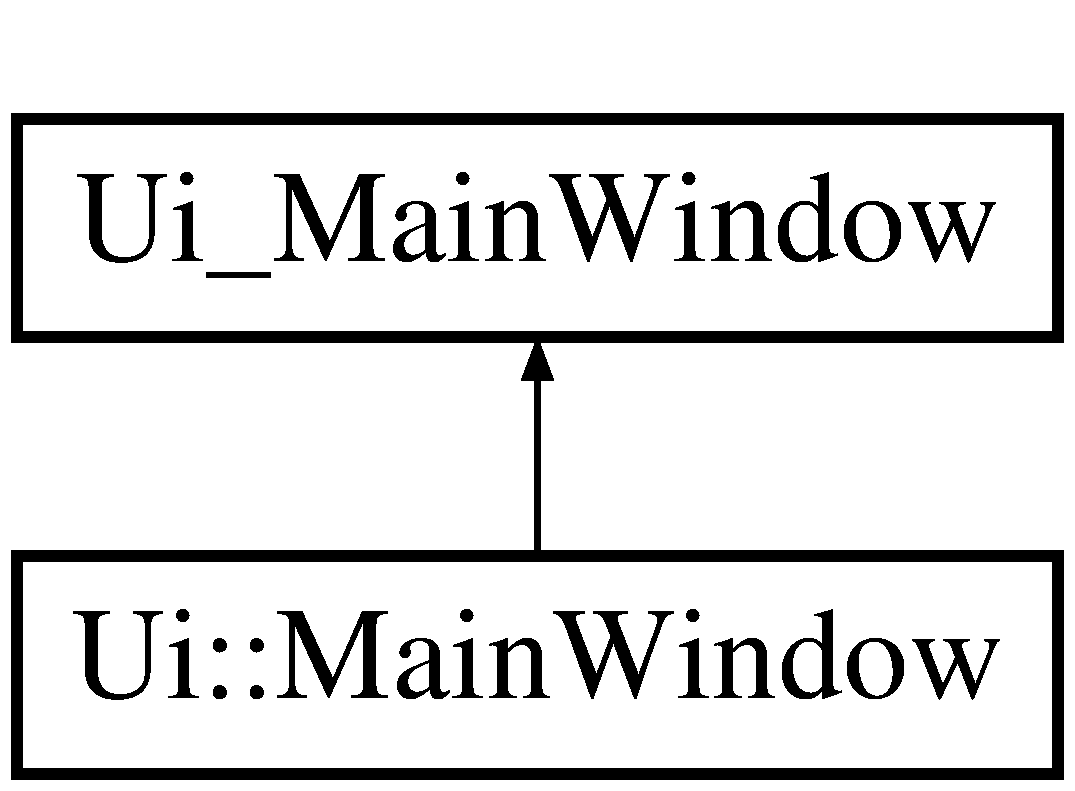
\includegraphics[height=2.000000cm]{class_ui_1_1_main_window}
\end{center}
\end{figure}


\subsection{\-Detailed \-Description}


\-Definition at line 482 of file ui\-\_\-mainwindow.\-h.



\-The documentation for this class was generated from the following file\-:\begin{DoxyCompactItemize}
\item 
/media/\-My\-Passport\-Blue/\-Data/\-Research/\-Simulations/\-Colony/\hyperlink{ui__mainwindow_8h}{ui\-\_\-mainwindow.\-h}\end{DoxyCompactItemize}

\hypertarget{class_milieu}{\section{\-Milieu \-Class \-Reference}
\label{class_milieu}\index{\-Milieu@{\-Milieu}}
}


{\ttfamily \#include $<$\-Milieu.\-h$>$}

\-Inheritance diagram for \-Milieu\-:\begin{figure}[H]
\begin{center}
\leavevmode
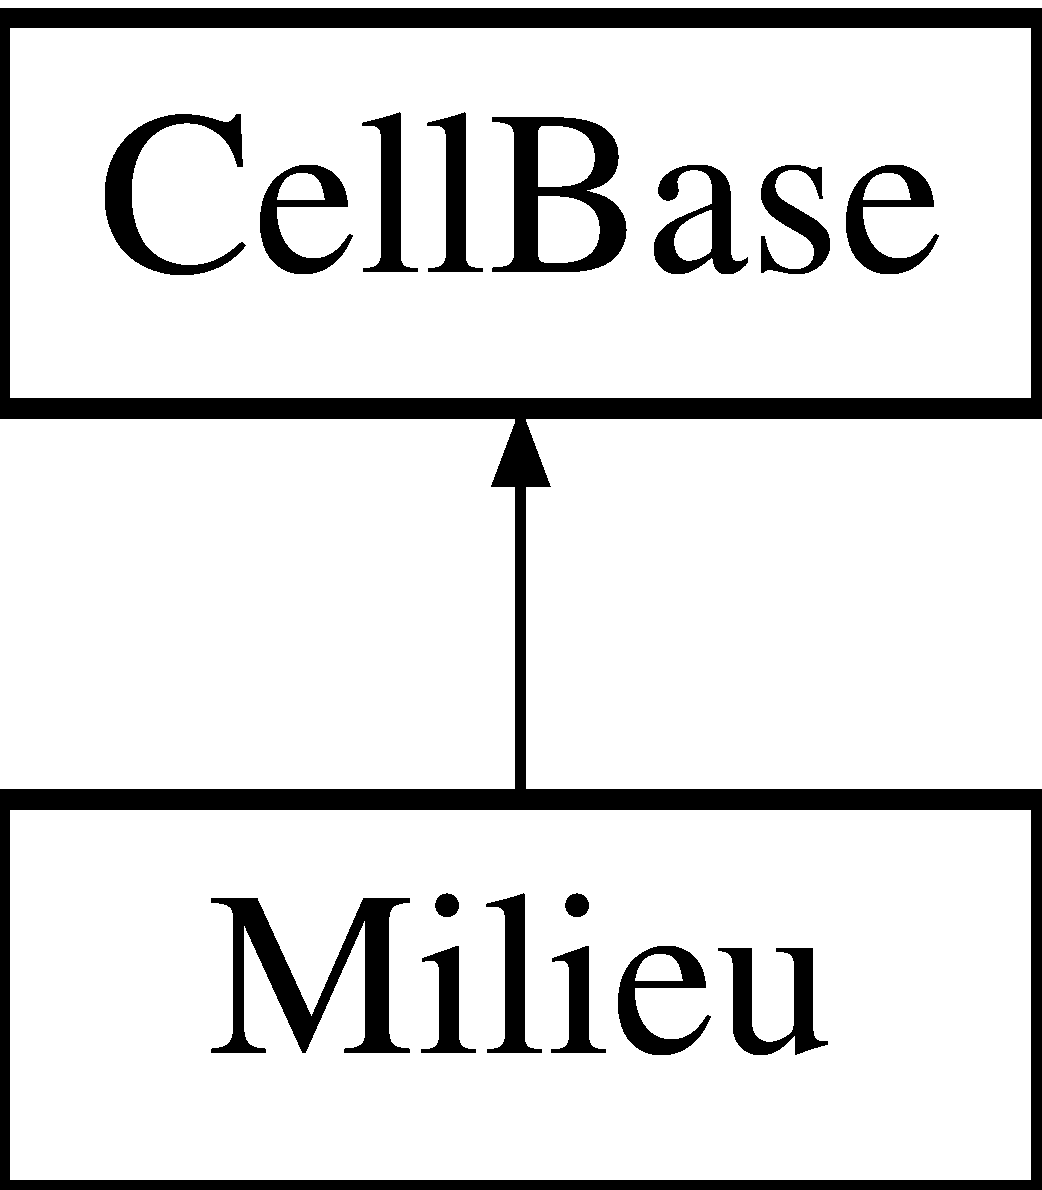
\includegraphics[height=2.000000cm]{class_milieu}
\end{center}
\end{figure}
\subsection*{\-Public \-Member \-Functions}
\begin{DoxyCompactItemize}
\item 
double \hyperlink{class_milieu_ad48c676f6943018da4d7dcab5c04a450}{get\-Time\-Dependent\-Volume} (const double time) const 
\end{DoxyCompactItemize}
\subsection*{\-Public \-Attributes}
\begin{DoxyCompactItemize}
\item 
double \hyperlink{class_milieu_add3fc66df8f106caf4eab9804b7e1210}{milieu\-Volume\-\_\-}
\end{DoxyCompactItemize}


\subsection{\-Detailed \-Description}
\-A special cell that represents the environment in which the colony of cells live. \-It can contain chemical species and reactions, like a normal \hyperlink{class_cell_base}{\-Cell\-Base} object and cannot divide. 

\-Definition at line 42 of file \-Milieu.\-h.



\subsection{\-Member \-Function \-Documentation}
\hypertarget{class_milieu_ad48c676f6943018da4d7dcab5c04a450}{\index{\-Milieu@{\-Milieu}!get\-Time\-Dependent\-Volume@{get\-Time\-Dependent\-Volume}}
\index{get\-Time\-Dependent\-Volume@{get\-Time\-Dependent\-Volume}!Milieu@{\-Milieu}}
\subsubsection[{get\-Time\-Dependent\-Volume}]{\setlength{\rightskip}{0pt plus 5cm}double {\bf \-Milieu\-::get\-Time\-Dependent\-Volume} (
\begin{DoxyParamCaption}
\item[{const double}]{time}
\end{DoxyParamCaption}
) const\hspace{0.3cm}{\ttfamily  \mbox{[}virtual\mbox{]}}}}\label{class_milieu_ad48c676f6943018da4d7dcab5c04a450}
\-We reimplement the method in order to return a value of the milieu volume independent of time and dependent only on the number of cells (volume0). \-This is an approximation since we should take into account the volume of all the other cells in order to calculate the volume of the milieu. \-However, as the volume of the milieu is much larger than the volume of one cell, there is not much difference. \-U\-P\-D\-A\-T\-E 2013.\-10.\-17\-: change this method in order to take into account the volume of \-A\-L\-L the cells and to compute exactly the volume of the milieu. \-Managed by \hyperlink{class_cell_collection}{\-Cell\-Collection} (this is easier since we have to know the volume of \-A\-L\-L the cells). \-We use a variable milieu\-Volume\-\_\- that we will only update at each time slice, trade-\/off between accuracy and computation time. \-Also, volume0 is now constant for the milieu and refers to the inital volume. 

\-Implements \hyperlink{class_cell_base_a7b69eec41c172b719e7f2ea6cb277ce9}{\-Cell\-Base}.



\-Definition at line 20 of file \-Milieu.\-cpp.



\subsection{\-Member \-Data \-Documentation}
\hypertarget{class_milieu_add3fc66df8f106caf4eab9804b7e1210}{\index{\-Milieu@{\-Milieu}!milieu\-Volume\-\_\-@{milieu\-Volume\-\_\-}}
\index{milieu\-Volume\-\_\-@{milieu\-Volume\-\_\-}!Milieu@{\-Milieu}}
\subsubsection[{milieu\-Volume\-\_\-}]{\setlength{\rightskip}{0pt plus 5cm}double {\bf \-Milieu\-::milieu\-Volume\-\_\-}}}\label{class_milieu_add3fc66df8f106caf4eab9804b7e1210}


\-Definition at line 62 of file \-Milieu.\-h.



\-The documentation for this class was generated from the following files\-:\begin{DoxyCompactItemize}
\item 
/media/\-My\-Passport\-Blue/\-Data/\-Research/\-Simulations/\-Colony/\hyperlink{_milieu_8h}{\-Milieu.\-h}\item 
/media/\-My\-Passport\-Blue/\-Data/\-Research/\-Simulations/\-Colony/\hyperlink{_milieu_8cpp}{\-Milieu.\-cpp}\end{DoxyCompactItemize}

\hypertarget{class_o_d_e_simulation}{\section{\-O\-D\-E\-Simulation \-Class \-Reference}
\label{class_o_d_e_simulation}\index{\-O\-D\-E\-Simulation@{\-O\-D\-E\-Simulation}}
}


{\ttfamily \#include $<$\-O\-D\-E\-Simulation.\-h$>$}

\-Inheritance diagram for \-O\-D\-E\-Simulation\-:\begin{figure}[H]
\begin{center}
\leavevmode
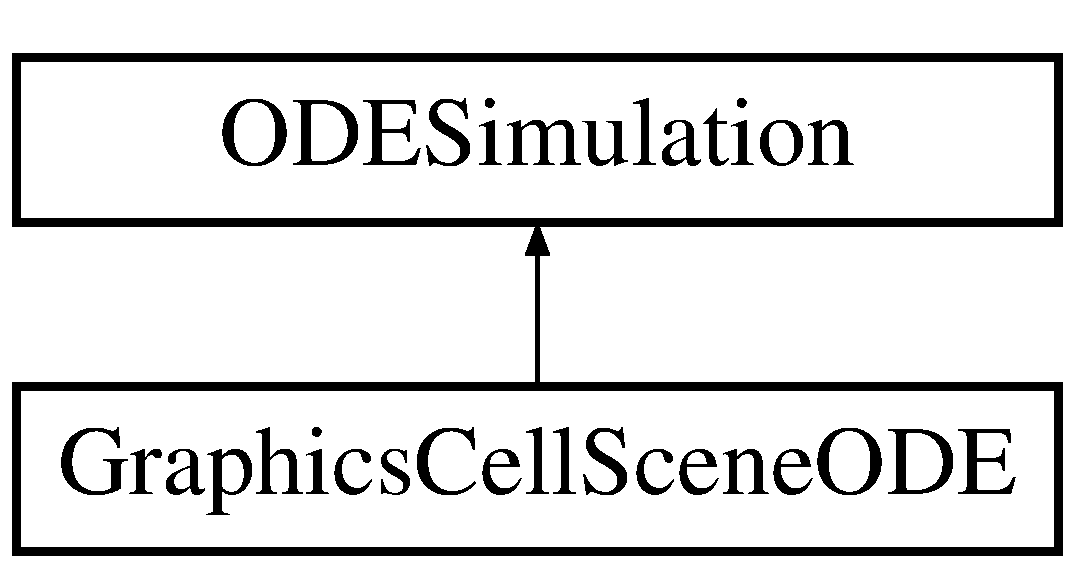
\includegraphics[height=2.000000cm]{class_o_d_e_simulation}
\end{center}
\end{figure}
\subsection*{\-Public \-Member \-Functions}
\begin{DoxyCompactItemize}
\item 
\hyperlink{class_o_d_e_simulation_ae594151b85a5528b8c9cc44e268c7256}{\-O\-D\-E\-Simulation} ()
\item 
\hyperlink{class_o_d_e_simulation_abaa90d10deb102d150497ca5db7f1af4}{$\sim$\-O\-D\-E\-Simulation} ()
\item 
d\-World\-I\-D \hyperlink{class_o_d_e_simulation_a9320cdf91a7e002119eb0cb0bba9c7b0}{get\-World} () const 
\item 
void \hyperlink{class_o_d_e_simulation_a83fbf3e98bab325948da3e4d1b3f3848}{init} ()
\item 
void \hyperlink{class_o_d_e_simulation_a5a72dab563d6c80d6643c1f940bb3349}{handle\-Collision\-Between} (d\-Geom\-I\-D o0, d\-Geom\-I\-D o1)
\end{DoxyCompactItemize}
\subsection*{\-Protected \-Member \-Functions}
\begin{DoxyCompactItemize}
\item 
virtual void \hyperlink{class_o_d_e_simulation_ac5ca4e063d5021dfbb6fd1b3d8004a8a}{compute\-Step} (float time\-Step, \-Q\-List$<$ \-Graphics\-Cell $\ast$ $>$ $\ast$cells\-List, double colony\-Size, bool equilibration, double average\-Cell\-Length, double cell\-Height)
\item 
void \hyperlink{class_o_d_e_simulation_a55e70b91c52db2998b169148c6e4b853}{compute\-Step\-With\-Aligning\-Force} (float time\-Step, \-Q\-List$<$ \-Graphics\-Cell $\ast$ $>$ $\ast$cells\-List, double colony\-Size)
\item 
void \hyperlink{class_o_d_e_simulation_a5e50af215ed7e46ec872d1fc7dc2cc7b}{compute\-Forces} (\-Q\-List$<$ \-Graphics\-Cell $\ast$ $>$ $\ast$cells\-List, double colony\-Size, bool low\-Friction)
\item 
void \hyperlink{class_o_d_e_simulation_a25eefbb4cafc5a920837f3469dcee977}{compute\-Aligning\-Forces} (\-Q\-List$<$ \-Graphics\-Cell $\ast$ $>$ $\ast$cells\-List, double colony\-Size)
\item 
double \hyperlink{class_o_d_e_simulation_a1a69251dfb38f5be8b7bc1947ea06f98}{compute\-Colony\-Radius} (\-Q\-List$<$ \-Graphics\-Cell $\ast$ $>$ $\ast$cells\-List, double colony\-Size)
\end{DoxyCompactItemize}
\subsection*{\-Protected \-Attributes}
\begin{DoxyCompactItemize}
\item 
d\-World\-I\-D \hyperlink{class_o_d_e_simulation_ab01265ac8b2ec870b00c35e017d9cd48}{world\-\_\-}
\item 
d\-Space\-I\-D \hyperlink{class_o_d_e_simulation_afe195e9dc824b0311b2959e8bd058c19}{space\-\_\-}
\end{DoxyCompactItemize}


\subsection{\-Detailed \-Description}
\-Open \-Dynamics \-Engine (\-O\-D\-E) simulation. \-Contains and defines the \-O\-D\-E world and the basics and the \-O\-D\-E simulation\-: simulation step method, computes forces between objects, handle collision method. 

\-Definition at line 39 of file \-O\-D\-E\-Simulation.\-h.



\subsection{\-Constructor \& \-Destructor \-Documentation}
\hypertarget{class_o_d_e_simulation_ae594151b85a5528b8c9cc44e268c7256}{\index{\-O\-D\-E\-Simulation@{\-O\-D\-E\-Simulation}!\-O\-D\-E\-Simulation@{\-O\-D\-E\-Simulation}}
\index{\-O\-D\-E\-Simulation@{\-O\-D\-E\-Simulation}!ODESimulation@{\-O\-D\-E\-Simulation}}
\subsubsection[{\-O\-D\-E\-Simulation}]{\setlength{\rightskip}{0pt plus 5cm}{\bf \-O\-D\-E\-Simulation\-::\-O\-D\-E\-Simulation} (
\begin{DoxyParamCaption}
{}
\end{DoxyParamCaption}
)}}\label{class_o_d_e_simulation_ae594151b85a5528b8c9cc44e268c7256}


\-Definition at line 30 of file \-O\-D\-E\-Simulation.\-cpp.

\hypertarget{class_o_d_e_simulation_abaa90d10deb102d150497ca5db7f1af4}{\index{\-O\-D\-E\-Simulation@{\-O\-D\-E\-Simulation}!$\sim$\-O\-D\-E\-Simulation@{$\sim$\-O\-D\-E\-Simulation}}
\index{$\sim$\-O\-D\-E\-Simulation@{$\sim$\-O\-D\-E\-Simulation}!ODESimulation@{\-O\-D\-E\-Simulation}}
\subsubsection[{$\sim$\-O\-D\-E\-Simulation}]{\setlength{\rightskip}{0pt plus 5cm}{\bf \-O\-D\-E\-Simulation\-::$\sim$\-O\-D\-E\-Simulation} (
\begin{DoxyParamCaption}
{}
\end{DoxyParamCaption}
)}}\label{class_o_d_e_simulation_abaa90d10deb102d150497ca5db7f1af4}


\-Definition at line 80 of file \-O\-D\-E\-Simulation.\-cpp.



\subsection{\-Member \-Function \-Documentation}
\hypertarget{class_o_d_e_simulation_a25eefbb4cafc5a920837f3469dcee977}{\index{\-O\-D\-E\-Simulation@{\-O\-D\-E\-Simulation}!compute\-Aligning\-Forces@{compute\-Aligning\-Forces}}
\index{compute\-Aligning\-Forces@{compute\-Aligning\-Forces}!ODESimulation@{\-O\-D\-E\-Simulation}}
\subsubsection[{compute\-Aligning\-Forces}]{\setlength{\rightskip}{0pt plus 5cm}void {\bf \-O\-D\-E\-Simulation\-::compute\-Aligning\-Forces} (
\begin{DoxyParamCaption}
\item[{\-Q\-List$<$ \-Graphics\-Cell $\ast$ $>$ $\ast$}]{cells\-List, }
\item[{double}]{colony\-Size}
\end{DoxyParamCaption}
)\hspace{0.3cm}{\ttfamily  \mbox{[}protected\mbox{]}}}}\label{class_o_d_e_simulation_a25eefbb4cafc5a920837f3469dcee977}


\-Definition at line 338 of file \-O\-D\-E\-Simulation.\-cpp.

\hypertarget{class_o_d_e_simulation_a1a69251dfb38f5be8b7bc1947ea06f98}{\index{\-O\-D\-E\-Simulation@{\-O\-D\-E\-Simulation}!compute\-Colony\-Radius@{compute\-Colony\-Radius}}
\index{compute\-Colony\-Radius@{compute\-Colony\-Radius}!ODESimulation@{\-O\-D\-E\-Simulation}}
\subsubsection[{compute\-Colony\-Radius}]{\setlength{\rightskip}{0pt plus 5cm}double {\bf \-O\-D\-E\-Simulation\-::compute\-Colony\-Radius} (
\begin{DoxyParamCaption}
\item[{\-Q\-List$<$ \-Graphics\-Cell $\ast$ $>$ $\ast$}]{cells\-List, }
\item[{double}]{colony\-Size}
\end{DoxyParamCaption}
)\hspace{0.3cm}{\ttfamily  \mbox{[}protected\mbox{]}}}}\label{class_o_d_e_simulation_a1a69251dfb38f5be8b7bc1947ea06f98}


\-Definition at line 402 of file \-O\-D\-E\-Simulation.\-cpp.

\hypertarget{class_o_d_e_simulation_a5e50af215ed7e46ec872d1fc7dc2cc7b}{\index{\-O\-D\-E\-Simulation@{\-O\-D\-E\-Simulation}!compute\-Forces@{compute\-Forces}}
\index{compute\-Forces@{compute\-Forces}!ODESimulation@{\-O\-D\-E\-Simulation}}
\subsubsection[{compute\-Forces}]{\setlength{\rightskip}{0pt plus 5cm}void {\bf \-O\-D\-E\-Simulation\-::compute\-Forces} (
\begin{DoxyParamCaption}
\item[{\-Q\-List$<$ \-Graphics\-Cell $\ast$ $>$ $\ast$}]{cells\-List, }
\item[{double}]{colony\-Size, }
\item[{bool}]{low\-Friction}
\end{DoxyParamCaption}
)\hspace{0.3cm}{\ttfamily  \mbox{[}protected\mbox{]}}}}\label{class_o_d_e_simulation_a5e50af215ed7e46ec872d1fc7dc2cc7b}


\-Definition at line 237 of file \-O\-D\-E\-Simulation.\-cpp.

\hypertarget{class_o_d_e_simulation_ac5ca4e063d5021dfbb6fd1b3d8004a8a}{\index{\-O\-D\-E\-Simulation@{\-O\-D\-E\-Simulation}!compute\-Step@{compute\-Step}}
\index{compute\-Step@{compute\-Step}!ODESimulation@{\-O\-D\-E\-Simulation}}
\subsubsection[{compute\-Step}]{\setlength{\rightskip}{0pt plus 5cm}void {\bf \-O\-D\-E\-Simulation\-::compute\-Step} (
\begin{DoxyParamCaption}
\item[{float}]{time\-Step, }
\item[{\-Q\-List$<$ \-Graphics\-Cell $\ast$ $>$ $\ast$}]{cells\-List, }
\item[{double}]{colony\-Size, }
\item[{bool}]{equilibration, }
\item[{double}]{average\-Cell\-Length, }
\item[{double}]{cell\-Height}
\end{DoxyParamCaption}
)\hspace{0.3cm}{\ttfamily  \mbox{[}protected, virtual\mbox{]}}}}\label{class_o_d_e_simulation_ac5ca4e063d5021dfbb6fd1b3d8004a8a}


\-Definition at line 96 of file \-O\-D\-E\-Simulation.\-cpp.

\hypertarget{class_o_d_e_simulation_a55e70b91c52db2998b169148c6e4b853}{\index{\-O\-D\-E\-Simulation@{\-O\-D\-E\-Simulation}!compute\-Step\-With\-Aligning\-Force@{compute\-Step\-With\-Aligning\-Force}}
\index{compute\-Step\-With\-Aligning\-Force@{compute\-Step\-With\-Aligning\-Force}!ODESimulation@{\-O\-D\-E\-Simulation}}
\subsubsection[{compute\-Step\-With\-Aligning\-Force}]{\setlength{\rightskip}{0pt plus 5cm}void {\bf \-O\-D\-E\-Simulation\-::compute\-Step\-With\-Aligning\-Force} (
\begin{DoxyParamCaption}
\item[{float}]{time\-Step, }
\item[{\-Q\-List$<$ \-Graphics\-Cell $\ast$ $>$ $\ast$}]{cells\-List, }
\item[{double}]{colony\-Size}
\end{DoxyParamCaption}
)\hspace{0.3cm}{\ttfamily  \mbox{[}protected\mbox{]}}}}\label{class_o_d_e_simulation_a55e70b91c52db2998b169148c6e4b853}


\-Definition at line 157 of file \-O\-D\-E\-Simulation.\-cpp.

\hypertarget{class_o_d_e_simulation_a9320cdf91a7e002119eb0cb0bba9c7b0}{\index{\-O\-D\-E\-Simulation@{\-O\-D\-E\-Simulation}!get\-World@{get\-World}}
\index{get\-World@{get\-World}!ODESimulation@{\-O\-D\-E\-Simulation}}
\subsubsection[{get\-World}]{\setlength{\rightskip}{0pt plus 5cm}d\-World\-I\-D {\bf \-O\-D\-E\-Simulation\-::get\-World} (
\begin{DoxyParamCaption}
{}
\end{DoxyParamCaption}
) const}}\label{class_o_d_e_simulation_a9320cdf91a7e002119eb0cb0bba9c7b0}


\-Definition at line 89 of file \-O\-D\-E\-Simulation.\-cpp.

\hypertarget{class_o_d_e_simulation_a5a72dab563d6c80d6643c1f940bb3349}{\index{\-O\-D\-E\-Simulation@{\-O\-D\-E\-Simulation}!handle\-Collision\-Between@{handle\-Collision\-Between}}
\index{handle\-Collision\-Between@{handle\-Collision\-Between}!ODESimulation@{\-O\-D\-E\-Simulation}}
\subsubsection[{handle\-Collision\-Between}]{\setlength{\rightskip}{0pt plus 5cm}void {\bf \-O\-D\-E\-Simulation\-::handle\-Collision\-Between} (
\begin{DoxyParamCaption}
\item[{d\-Geom\-I\-D}]{o0, }
\item[{d\-Geom\-I\-D}]{o1}
\end{DoxyParamCaption}
)}}\label{class_o_d_e_simulation_a5a72dab563d6c80d6643c1f940bb3349}


\-Definition at line 189 of file \-O\-D\-E\-Simulation.\-cpp.

\hypertarget{class_o_d_e_simulation_a83fbf3e98bab325948da3e4d1b3f3848}{\index{\-O\-D\-E\-Simulation@{\-O\-D\-E\-Simulation}!init@{init}}
\index{init@{init}!ODESimulation@{\-O\-D\-E\-Simulation}}
\subsubsection[{init}]{\setlength{\rightskip}{0pt plus 5cm}void {\bf \-O\-D\-E\-Simulation\-::init} (
\begin{DoxyParamCaption}
{}
\end{DoxyParamCaption}
)}}\label{class_o_d_e_simulation_a83fbf3e98bab325948da3e4d1b3f3848}


\-Definition at line 74 of file \-O\-D\-E\-Simulation.\-cpp.



\subsection{\-Member \-Data \-Documentation}
\hypertarget{class_o_d_e_simulation_afe195e9dc824b0311b2959e8bd058c19}{\index{\-O\-D\-E\-Simulation@{\-O\-D\-E\-Simulation}!space\-\_\-@{space\-\_\-}}
\index{space\-\_\-@{space\-\_\-}!ODESimulation@{\-O\-D\-E\-Simulation}}
\subsubsection[{space\-\_\-}]{\setlength{\rightskip}{0pt plus 5cm}d\-Space\-I\-D {\bf \-O\-D\-E\-Simulation\-::space\-\_\-}\hspace{0.3cm}{\ttfamily  \mbox{[}protected\mbox{]}}}}\label{class_o_d_e_simulation_afe195e9dc824b0311b2959e8bd058c19}


\-Definition at line 54 of file \-O\-D\-E\-Simulation.\-h.

\hypertarget{class_o_d_e_simulation_ab01265ac8b2ec870b00c35e017d9cd48}{\index{\-O\-D\-E\-Simulation@{\-O\-D\-E\-Simulation}!world\-\_\-@{world\-\_\-}}
\index{world\-\_\-@{world\-\_\-}!ODESimulation@{\-O\-D\-E\-Simulation}}
\subsubsection[{world\-\_\-}]{\setlength{\rightskip}{0pt plus 5cm}d\-World\-I\-D {\bf \-O\-D\-E\-Simulation\-::world\-\_\-}\hspace{0.3cm}{\ttfamily  \mbox{[}protected\mbox{]}}}}\label{class_o_d_e_simulation_ab01265ac8b2ec870b00c35e017d9cd48}


\-Definition at line 53 of file \-O\-D\-E\-Simulation.\-h.



\-The documentation for this class was generated from the following files\-:\begin{DoxyCompactItemize}
\item 
/media/\-My\-Passport\-Blue/\-Data/\-Research/\-Simulations/\-Colony/\hyperlink{_o_d_e_simulation_8h}{\-O\-D\-E\-Simulation.\-h}\item 
/media/\-My\-Passport\-Blue/\-Data/\-Research/\-Simulations/\-Colony/\hyperlink{_o_d_e_simulation_8cpp}{\-O\-D\-E\-Simulation.\-cpp}\end{DoxyCompactItemize}

\hypertarget{class_output}{\section{\-Output \-Class \-Reference}
\label{class_output}\index{\-Output@{\-Output}}
}


{\ttfamily \#include $<$\-Output.\-h$>$}

\subsection*{\-Public \-Member \-Functions}
\begin{DoxyCompactItemize}
\item 
\hyperlink{class_output_a428c663520336477a12f1a33504eb067}{\-Output} ()
\item 
\hyperlink{class_output_a61d0840daf98bea49e4dc471f235eeab}{$\sim$\-Output} ()
\item 
void \hyperlink{class_output_a656d3b4d04355381c544851ced239100}{initialize} (const \hyperlink{class_input}{\-Input} \&p)
\item 
void \hyperlink{class_output_a77417156c6f8d8488d4d4ef4f908195f}{write\-Time\-Mesh\-Trajectory} (list$<$ \hyperlink{class_time_slice}{\-Time\-Slice} $>$ \&time\-Mesh\-Trajectory, int i\-Traj, bool is\-Enabled\-Compute\-Spatial\-Dynamics)
\item 
void \hyperlink{class_output_a83c90262752ea2e4b25a54779d4dc754}{write\-Time\-Mesh\-Cells\-Avg} (\-Array$<$ \hyperlink{class_time_slice_cells_avg}{\-Time\-Slice\-Cells\-Avg}, 1 $>$ \&time\-Mesh\-Cells\-Avg, int i\-Traj)
\item 
void \hyperlink{class_output_a16624e8c9b13271f7ace2bbb217430db}{write\-Cell\-Lineage} (list$<$ \hyperlink{class_cell_lineage_generation}{\-Cell\-Lineage\-Generation} $>$ cell\-Lineage, int i\-Traj)
\item 
void \hyperlink{class_output_a8daec3ace3c03412d627af6f791332e2}{write\-Time\-Mesh\-Cells\-Trajectories\-Avg} (\-Array$<$ \hyperlink{class_time_slice_cells_avg}{\-Time\-Slice\-Cells\-Avg}, 1 $>$ \&time\-Mesh\-Cells\-Trajectories\-Avg)
\item 
void \hyperlink{class_output_a74bd96aeaab227064791019cfaa1c7ef}{write\-Cell\-Cycle\-Phases} (\-Array$<$ double, 1 $>$ cell\-Cycle\-Phases)
\item 
void \hyperlink{class_output_a6312626943f77b1dc780b60e2b476bbd}{write\-First\-Passage\-Time} (\-Array$<$ double, 1 $>$ \&first\-Passage\-Time\-Values)
\item 
void \hyperlink{class_output_a8ad983d5d1526a180e3a9cdb005b4198}{close} ()
\end{DoxyCompactItemize}


\subsection{\-Detailed \-Description}
\-Output class with methods to write output files. 

\-Definition at line 67 of file \-Output.\-h.



\subsection{\-Constructor \& \-Destructor \-Documentation}
\hypertarget{class_output_a428c663520336477a12f1a33504eb067}{\index{\-Output@{\-Output}!\-Output@{\-Output}}
\index{\-Output@{\-Output}!Output@{\-Output}}
\subsubsection[{\-Output}]{\setlength{\rightskip}{0pt plus 5cm}{\bf \-Output\-::\-Output} (
\begin{DoxyParamCaption}
{}
\end{DoxyParamCaption}
)}}\label{class_output_a428c663520336477a12f1a33504eb067}
\-Default constructor. 

\-Definition at line 20 of file \-Output.\-cpp.

\hypertarget{class_output_a61d0840daf98bea49e4dc471f235eeab}{\index{\-Output@{\-Output}!$\sim$\-Output@{$\sim$\-Output}}
\index{$\sim$\-Output@{$\sim$\-Output}!Output@{\-Output}}
\subsubsection[{$\sim$\-Output}]{\setlength{\rightskip}{0pt plus 5cm}{\bf \-Output\-::$\sim$\-Output} (
\begin{DoxyParamCaption}
{}
\end{DoxyParamCaption}
)}}\label{class_output_a61d0840daf98bea49e4dc471f235eeab}


\-Definition at line 25 of file \-Output.\-cpp.



\subsection{\-Member \-Function \-Documentation}
\hypertarget{class_output_a8ad983d5d1526a180e3a9cdb005b4198}{\index{\-Output@{\-Output}!close@{close}}
\index{close@{close}!Output@{\-Output}}
\subsubsection[{close}]{\setlength{\rightskip}{0pt plus 5cm}void {\bf \-Output\-::close} (
\begin{DoxyParamCaption}
{}
\end{DoxyParamCaption}
)}}\label{class_output_a8ad983d5d1526a180e3a9cdb005b4198}


\-Definition at line 128 of file \-Output.\-cpp.

\hypertarget{class_output_a656d3b4d04355381c544851ced239100}{\index{\-Output@{\-Output}!initialize@{initialize}}
\index{initialize@{initialize}!Output@{\-Output}}
\subsubsection[{initialize}]{\setlength{\rightskip}{0pt plus 5cm}void {\bf \-Output\-::initialize} (
\begin{DoxyParamCaption}
\item[{const {\bf \-Input} \&}]{p}
\end{DoxyParamCaption}
)}}\label{class_output_a656d3b4d04355381c544851ced239100}


\-Definition at line 34 of file \-Output.\-cpp.

\hypertarget{class_output_a74bd96aeaab227064791019cfaa1c7ef}{\index{\-Output@{\-Output}!write\-Cell\-Cycle\-Phases@{write\-Cell\-Cycle\-Phases}}
\index{write\-Cell\-Cycle\-Phases@{write\-Cell\-Cycle\-Phases}!Output@{\-Output}}
\subsubsection[{write\-Cell\-Cycle\-Phases}]{\setlength{\rightskip}{0pt plus 5cm}void {\bf \-Output\-::write\-Cell\-Cycle\-Phases} (
\begin{DoxyParamCaption}
\item[{\-Array$<$ double, 1 $>$}]{cell\-Cycle\-Phases}
\end{DoxyParamCaption}
)}}\label{class_output_a74bd96aeaab227064791019cfaa1c7ef}


\-Definition at line 413 of file \-Output.\-cpp.

\hypertarget{class_output_a16624e8c9b13271f7ace2bbb217430db}{\index{\-Output@{\-Output}!write\-Cell\-Lineage@{write\-Cell\-Lineage}}
\index{write\-Cell\-Lineage@{write\-Cell\-Lineage}!Output@{\-Output}}
\subsubsection[{write\-Cell\-Lineage}]{\setlength{\rightskip}{0pt plus 5cm}void {\bf \-Output\-::write\-Cell\-Lineage} (
\begin{DoxyParamCaption}
\item[{list$<$ {\bf \-Cell\-Lineage\-Generation} $>$}]{cell\-Lineage, }
\item[{int}]{i\-Traj}
\end{DoxyParamCaption}
)}}\label{class_output_a16624e8c9b13271f7ace2bbb217430db}


\-Definition at line 329 of file \-Output.\-cpp.

\hypertarget{class_output_a6312626943f77b1dc780b60e2b476bbd}{\index{\-Output@{\-Output}!write\-First\-Passage\-Time@{write\-First\-Passage\-Time}}
\index{write\-First\-Passage\-Time@{write\-First\-Passage\-Time}!Output@{\-Output}}
\subsubsection[{write\-First\-Passage\-Time}]{\setlength{\rightskip}{0pt plus 5cm}void {\bf \-Output\-::write\-First\-Passage\-Time} (
\begin{DoxyParamCaption}
\item[{\-Array$<$ double, 1 $>$ \&}]{first\-Passage\-Time\-Values}
\end{DoxyParamCaption}
)}}\label{class_output_a6312626943f77b1dc780b60e2b476bbd}


\-Definition at line 439 of file \-Output.\-cpp.

\hypertarget{class_output_a83c90262752ea2e4b25a54779d4dc754}{\index{\-Output@{\-Output}!write\-Time\-Mesh\-Cells\-Avg@{write\-Time\-Mesh\-Cells\-Avg}}
\index{write\-Time\-Mesh\-Cells\-Avg@{write\-Time\-Mesh\-Cells\-Avg}!Output@{\-Output}}
\subsubsection[{write\-Time\-Mesh\-Cells\-Avg}]{\setlength{\rightskip}{0pt plus 5cm}void {\bf \-Output\-::write\-Time\-Mesh\-Cells\-Avg} (
\begin{DoxyParamCaption}
\item[{\-Array$<$ {\bf \-Time\-Slice\-Cells\-Avg}, 1 $>$ \&}]{time\-Mesh\-Cells\-Avg, }
\item[{int}]{i\-Traj}
\end{DoxyParamCaption}
)}}\label{class_output_a83c90262752ea2e4b25a54779d4dc754}


\-Definition at line 284 of file \-Output.\-cpp.

\hypertarget{class_output_a8daec3ace3c03412d627af6f791332e2}{\index{\-Output@{\-Output}!write\-Time\-Mesh\-Cells\-Trajectories\-Avg@{write\-Time\-Mesh\-Cells\-Trajectories\-Avg}}
\index{write\-Time\-Mesh\-Cells\-Trajectories\-Avg@{write\-Time\-Mesh\-Cells\-Trajectories\-Avg}!Output@{\-Output}}
\subsubsection[{write\-Time\-Mesh\-Cells\-Trajectories\-Avg}]{\setlength{\rightskip}{0pt plus 5cm}void {\bf \-Output\-::write\-Time\-Mesh\-Cells\-Trajectories\-Avg} (
\begin{DoxyParamCaption}
\item[{\-Array$<$ {\bf \-Time\-Slice\-Cells\-Avg}, 1 $>$ \&}]{time\-Mesh\-Cells\-Trajectories\-Avg}
\end{DoxyParamCaption}
)}}\label{class_output_a8daec3ace3c03412d627af6f791332e2}


\-Definition at line 374 of file \-Output.\-cpp.

\hypertarget{class_output_a77417156c6f8d8488d4d4ef4f908195f}{\index{\-Output@{\-Output}!write\-Time\-Mesh\-Trajectory@{write\-Time\-Mesh\-Trajectory}}
\index{write\-Time\-Mesh\-Trajectory@{write\-Time\-Mesh\-Trajectory}!Output@{\-Output}}
\subsubsection[{write\-Time\-Mesh\-Trajectory}]{\setlength{\rightskip}{0pt plus 5cm}void {\bf \-Output\-::write\-Time\-Mesh\-Trajectory} (
\begin{DoxyParamCaption}
\item[{list$<$ {\bf \-Time\-Slice} $>$ \&}]{time\-Mesh\-Trajectory, }
\item[{int}]{i\-Traj, }
\item[{bool}]{is\-Enabled\-Compute\-Spatial\-Dynamics}
\end{DoxyParamCaption}
)}}\label{class_output_a77417156c6f8d8488d4d4ef4f908195f}


\-Definition at line 137 of file \-Output.\-cpp.



\-The documentation for this class was generated from the following files\-:\begin{DoxyCompactItemize}
\item 
/media/\-My\-Passport\-Blue/\-Data/\-Research/\-Simulations/\-Colony/\hyperlink{_output_8h}{\-Output.\-h}\item 
/media/\-My\-Passport\-Blue/\-Data/\-Research/\-Simulations/\-Colony/\hyperlink{_output_8cpp}{\-Output.\-cpp}\end{DoxyCompactItemize}

\hypertarget{class_random_number_generator}{\section{\-Random\-Number\-Generator \-Class \-Reference}
\label{class_random_number_generator}\index{\-Random\-Number\-Generator@{\-Random\-Number\-Generator}}
}


{\ttfamily \#include $<$\-Random\-Number\-Generator.\-h$>$}

\subsection*{\-Public \-Member \-Functions}
\begin{DoxyCompactItemize}
\item 
\hyperlink{class_random_number_generator_a8e7e711ea58f13f3ed95becbe33684e9}{\-Random\-Number\-Generator} ()
\item 
\hyperlink{class_random_number_generator_af4949b4234bd8d8283028162f8a8e7f5}{$\sim$\-Random\-Number\-Generator} ()
\end{DoxyCompactItemize}
\subsection*{\-Static \-Public \-Member \-Functions}
\begin{DoxyCompactItemize}
\item 
static void \hyperlink{class_random_number_generator_a7f9ac1a577f5f72fd07b5e769f232fbe}{initialize} ()
\item 
static void \hyperlink{class_random_number_generator_a16d763e85961dddeeebee1be0fc8a3a2}{initialize} (int seed)
\item 
static double \hyperlink{class_random_number_generator_a4f452a69c4f0fd0044979e3eea6ef358}{get\-Uniform} ()
\item 
static double \hyperlink{class_random_number_generator_adc771ab86d212e8d42fe4108d8a1a350}{get\-Normal} ()
\item 
static int \hyperlink{class_random_number_generator_afbb6020f2d5d13d08ce12256370d6408}{get\-Binomial} (double p, unsigned int n)
\item 
static double \hyperlink{class_random_number_generator_a4a8e5b43607e3d3d406bdc4f07ca3567}{get\-Cell\-Cycle} (double tdet, double gamma)
\end{DoxyCompactItemize}
\subsection*{\-Static \-Public \-Attributes}
\begin{DoxyCompactItemize}
\item 
static int \hyperlink{class_random_number_generator_a7a5c2be0f01f6265dee7285bc511f956}{n\-Lux\-I\-Exp\-\_\-} = 0
\end{DoxyCompactItemize}


\subsection{\-Detailed \-Description}
\-Random number generator from the \-G\-S\-L library. 

\-Definition at line 52 of file \-Random\-Number\-Generator.\-h.



\subsection{\-Constructor \& \-Destructor \-Documentation}
\hypertarget{class_random_number_generator_a8e7e711ea58f13f3ed95becbe33684e9}{\index{\-Random\-Number\-Generator@{\-Random\-Number\-Generator}!\-Random\-Number\-Generator@{\-Random\-Number\-Generator}}
\index{\-Random\-Number\-Generator@{\-Random\-Number\-Generator}!RandomNumberGenerator@{\-Random\-Number\-Generator}}
\subsubsection[{\-Random\-Number\-Generator}]{\setlength{\rightskip}{0pt plus 5cm}{\bf \-Random\-Number\-Generator\-::\-Random\-Number\-Generator} (
\begin{DoxyParamCaption}
{}
\end{DoxyParamCaption}
)}}\label{class_random_number_generator_a8e7e711ea58f13f3ed95becbe33684e9}


\-Definition at line 26 of file \-Random\-Number\-Generator.\-cpp.

\hypertarget{class_random_number_generator_af4949b4234bd8d8283028162f8a8e7f5}{\index{\-Random\-Number\-Generator@{\-Random\-Number\-Generator}!$\sim$\-Random\-Number\-Generator@{$\sim$\-Random\-Number\-Generator}}
\index{$\sim$\-Random\-Number\-Generator@{$\sim$\-Random\-Number\-Generator}!RandomNumberGenerator@{\-Random\-Number\-Generator}}
\subsubsection[{$\sim$\-Random\-Number\-Generator}]{\setlength{\rightskip}{0pt plus 5cm}{\bf \-Random\-Number\-Generator\-::$\sim$\-Random\-Number\-Generator} (
\begin{DoxyParamCaption}
{}
\end{DoxyParamCaption}
)}}\label{class_random_number_generator_af4949b4234bd8d8283028162f8a8e7f5}


\-Definition at line 31 of file \-Random\-Number\-Generator.\-cpp.



\subsection{\-Member \-Function \-Documentation}
\hypertarget{class_random_number_generator_afbb6020f2d5d13d08ce12256370d6408}{\index{\-Random\-Number\-Generator@{\-Random\-Number\-Generator}!get\-Binomial@{get\-Binomial}}
\index{get\-Binomial@{get\-Binomial}!RandomNumberGenerator@{\-Random\-Number\-Generator}}
\subsubsection[{get\-Binomial}]{\setlength{\rightskip}{0pt plus 5cm}int {\bf \-Random\-Number\-Generator\-::get\-Binomial} (
\begin{DoxyParamCaption}
\item[{double}]{p, }
\item[{unsigned int}]{n}
\end{DoxyParamCaption}
)\hspace{0.3cm}{\ttfamily  \mbox{[}inline, static\mbox{]}}}}\label{class_random_number_generator_afbb6020f2d5d13d08ce12256370d6408}
\-Returns a random integer from the binomial distribution, the number of successes in {\ttfamily n} independent trials with probability {\ttfamily p}. 

\-Definition at line 143 of file \-Random\-Number\-Generator.\-h.

\hypertarget{class_random_number_generator_a4a8e5b43607e3d3d406bdc4f07ca3567}{\index{\-Random\-Number\-Generator@{\-Random\-Number\-Generator}!get\-Cell\-Cycle@{get\-Cell\-Cycle}}
\index{get\-Cell\-Cycle@{get\-Cell\-Cycle}!RandomNumberGenerator@{\-Random\-Number\-Generator}}
\subsubsection[{get\-Cell\-Cycle}]{\setlength{\rightskip}{0pt plus 5cm}double {\bf \-Random\-Number\-Generator\-::get\-Cell\-Cycle} (
\begin{DoxyParamCaption}
\item[{double}]{tdet, }
\item[{double}]{gamma}
\end{DoxyParamCaption}
)\hspace{0.3cm}{\ttfamily  \mbox{[}static\mbox{]}}}}\label{class_random_number_generator_a4a8e5b43607e3d3d406bdc4f07ca3567}
\-Returns a random value for the cell cycle $t_c$. \-It is given by\-: \[ t_c = \gamma t_{det} + (1-\gamma)t_{sto} \] where $t_{det}$ and $t_{sto}$ are the deterministic and stochastic components of the cell cycle respectively, and $\gamma\in [0,1]$ is a parameter that weight their relative importance. \-Note that we acknowledge the fact that, prior to division, cells must mature and grow and consequently the cell cycle has a minimum duration $\gamma t_{det}$. \-The stochastic part, $t_{sto}$, is supposed to be exponentially distributed and its probability density reads, \[ \rho(t_{sto}) = \frac{1}{t_{det}} e^{-\frac{t_{sto}}{t_{det}}} \] \-Note that\-: \[ <\tau> = t_{det} \] \[ \sigma_{\tau} = (1-\gamma) t_{det} \] 

\-Definition at line 70 of file \-Random\-Number\-Generator.\-cpp.

\hypertarget{class_random_number_generator_adc771ab86d212e8d42fe4108d8a1a350}{\index{\-Random\-Number\-Generator@{\-Random\-Number\-Generator}!get\-Normal@{get\-Normal}}
\index{get\-Normal@{get\-Normal}!RandomNumberGenerator@{\-Random\-Number\-Generator}}
\subsubsection[{get\-Normal}]{\setlength{\rightskip}{0pt plus 5cm}double {\bf \-Random\-Number\-Generator\-::get\-Normal} (
\begin{DoxyParamCaption}
{}
\end{DoxyParamCaption}
)\hspace{0.3cm}{\ttfamily  \mbox{[}inline, static\mbox{]}}}}\label{class_random_number_generator_adc771ab86d212e8d42fe4108d8a1a350}
\-Returns a random number with normal distribution \-N(0,1). 

\-Definition at line 140 of file \-Random\-Number\-Generator.\-h.

\hypertarget{class_random_number_generator_a4f452a69c4f0fd0044979e3eea6ef358}{\index{\-Random\-Number\-Generator@{\-Random\-Number\-Generator}!get\-Uniform@{get\-Uniform}}
\index{get\-Uniform@{get\-Uniform}!RandomNumberGenerator@{\-Random\-Number\-Generator}}
\subsubsection[{get\-Uniform}]{\setlength{\rightskip}{0pt plus 5cm}double {\bf \-Random\-Number\-Generator\-::get\-Uniform} (
\begin{DoxyParamCaption}
{}
\end{DoxyParamCaption}
)\hspace{0.3cm}{\ttfamily  \mbox{[}inline, static\mbox{]}}}}\label{class_random_number_generator_a4f452a69c4f0fd0044979e3eea6ef358}
\-Returns a double in \mbox{[}0,1) with uniform probability. 

\-Definition at line 136 of file \-Random\-Number\-Generator.\-h.

\hypertarget{class_random_number_generator_a7f9ac1a577f5f72fd07b5e769f232fbe}{\index{\-Random\-Number\-Generator@{\-Random\-Number\-Generator}!initialize@{initialize}}
\index{initialize@{initialize}!RandomNumberGenerator@{\-Random\-Number\-Generator}}
\subsubsection[{initialize}]{\setlength{\rightskip}{0pt plus 5cm}void {\bf \-Random\-Number\-Generator\-::initialize} (
\begin{DoxyParamCaption}
{}
\end{DoxyParamCaption}
)\hspace{0.3cm}{\ttfamily  \mbox{[}static\mbox{]}}}}\label{class_random_number_generator_a7f9ac1a577f5f72fd07b5e769f232fbe}
\-Initiate the random number generator with a clock-\/cycle based seed. 

\-Definition at line 36 of file \-Random\-Number\-Generator.\-cpp.

\hypertarget{class_random_number_generator_a16d763e85961dddeeebee1be0fc8a3a2}{\index{\-Random\-Number\-Generator@{\-Random\-Number\-Generator}!initialize@{initialize}}
\index{initialize@{initialize}!RandomNumberGenerator@{\-Random\-Number\-Generator}}
\subsubsection[{initialize}]{\setlength{\rightskip}{0pt plus 5cm}void {\bf \-Random\-Number\-Generator\-::initialize} (
\begin{DoxyParamCaption}
\item[{int}]{seed}
\end{DoxyParamCaption}
)\hspace{0.3cm}{\ttfamily  \mbox{[}static\mbox{]}}}}\label{class_random_number_generator_a16d763e85961dddeeebee1be0fc8a3a2}
\-Initiate the random number generator with user defined seed. 

\-Definition at line 51 of file \-Random\-Number\-Generator.\-cpp.



\subsection{\-Member \-Data \-Documentation}
\hypertarget{class_random_number_generator_a7a5c2be0f01f6265dee7285bc511f956}{\index{\-Random\-Number\-Generator@{\-Random\-Number\-Generator}!n\-Lux\-I\-Exp\-\_\-@{n\-Lux\-I\-Exp\-\_\-}}
\index{n\-Lux\-I\-Exp\-\_\-@{n\-Lux\-I\-Exp\-\_\-}!RandomNumberGenerator@{\-Random\-Number\-Generator}}
\subsubsection[{n\-Lux\-I\-Exp\-\_\-}]{\setlength{\rightskip}{0pt plus 5cm}int {\bf \-Random\-Number\-Generator\-::n\-Lux\-I\-Exp\-\_\-} = 0\hspace{0.3cm}{\ttfamily  \mbox{[}static\mbox{]}}}}\label{class_random_number_generator_a7a5c2be0f01f6265dee7285bc511f956}


\-Definition at line 131 of file \-Random\-Number\-Generator.\-h.



\-The documentation for this class was generated from the following files\-:\begin{DoxyCompactItemize}
\item 
/media/\-My\-Passport\-Blue/\-Data/\-Research/\-Simulations/\-Colony/\hyperlink{_random_number_generator_8h}{\-Random\-Number\-Generator.\-h}\item 
/media/\-My\-Passport\-Blue/\-Data/\-Research/\-Simulations/\-Colony/\hyperlink{_random_number_generator_8cpp}{\-Random\-Number\-Generator.\-cpp}\end{DoxyCompactItemize}

\hypertarget{class_simulator}{\section{\-Simulator \-Class \-Reference}
\label{class_simulator}\index{\-Simulator@{\-Simulator}}
}


{\ttfamily \#include $<$\-Simulator.\-h$>$}

\subsection*{\-Public \-Member \-Functions}
\begin{DoxyCompactItemize}
\item 
void \hyperlink{class_simulator_a630ca1f9cba087798058d6b0d5c8564d}{init} ()
\item 
\hyperlink{class_simulator_a87d9ec0595c4f4953e3e59a1bdbd650a}{\-Simulator} (string input\-File)
\item 
\hyperlink{class_simulator_a7bc3104a9e0a2ea81f49f5dd2be6d7a7}{\-Simulator} (string input\-File, \-Graphics\-Cell\-Composite\-Param \&graphics\-Cell\-Param)
\item 
\hyperlink{class_simulator_a0f49aa04f42060a785adf77346b9de9f}{$\sim$\-Simulator} ()
\item 
void \hyperlink{class_simulator_a086254d2ac4f05260295cf6d39b39118}{init\-Main\-Window\-Param} (\-Graphics\-Cell\-Composite\-Param \&graphics\-Cell\-Param)
\item 
void \hyperlink{class_simulator_a050a8284ace34c39f271302d3fee80d3}{init\-Graphics\-Cell\-O\-D\-E\-Param} ()
\item 
double \hyperlink{class_simulator_a52361b7628b32d91da4ba369306f40e9}{get\-Time} () const 
\item 
double \hyperlink{class_simulator_a1d8fc1bc934ee5f41895d5ba4037002d}{get\-Simulation\-Time} () const 
\item 
\-Array$<$ double, 1 $>$ \hyperlink{class_simulator_ab26592212e1d456bd976f544e714fd13}{get\-Time\-Mesh} () const 
\item 
int \hyperlink{class_simulator_a3292a9420792a1267bd8ea6063931919}{get\-I\-Time\-Slice} () const 
\item 
int \hyperlink{class_simulator_a43e1b0569b932bf353b77f70daf95fbe}{get\-N\-Time\-Slice} () const 
\item 
int \hyperlink{class_simulator_a0ec57d427d83931c107009024fd09985}{get\-N\-Trajectory} () const 
\item 
int \hyperlink{class_simulator_ae9171c45b06669041e56a9278da1419f}{get\-I\-Trajectory} () const 
\item 
int \hyperlink{class_simulator_af9ed84ef1153ebcec61e0c629f07bc31}{get\-N\-Parameter\-Set} () const 
\item 
int \hyperlink{class_simulator_adbebc2a8b4fad6658b3c80ea37ba3fcc}{get\-I\-Parameter\-Set} () const 
\item 
int \hyperlink{class_simulator_af85b8999558e321b94d009f51ca23d63}{get\-N\-Global\-Parameter} () const 
\item 
\-Array$<$ double, 1 $>$ \hyperlink{class_simulator_acb6e9b058f821841e10dd4cf1a006a41}{get\-Global\-Parameter\-Array} () const 
\item 
vector$<$ string $>$ \hyperlink{class_simulator_a31fd30698c9596156e8e2388dde02d11}{getlist\-Global\-Parameters\-Name} () const 
\item 
\-Array$<$ double, 1 $>$ \hyperlink{class_simulator_a2c10cbe98ff0f710e6a15e4a40a8a0f7}{get\-Cells\-Angle} () const 
\item 
\-Array$<$ \-Tiny\-Vector$<$ double, 3 $>$, 1 $>$ \hyperlink{class_simulator_ac13cfded15101afabf0fd2a1d4a275ca}{get\-Cells\-Position} () const 
\item 
double \hyperlink{class_simulator_ac9d7febdac1bb6af0246230516084a85}{get\-Spatial\-Dynamics\-Equilibration\-Time} () const 
\item 
void \hyperlink{class_simulator_a68c747d0d0bf72ed3aae13f1fb256ff9}{initialize\-Cell\-Collection} ()
\item 
void \hyperlink{class_simulator_a46cc81d1c999a6b74dea75d0d3165e5f}{increase\-Time} (double t1)
\item 
void \hyperlink{class_simulator_ae425bfd3eb66830a3aed9e7d8ec2e04c}{set\-Time} (double t1)
\item 
void \hyperlink{class_simulator_a916ddb59f9208acb0dbe40ab2a653a46}{set\-Is\-Equilibration\-Steps} (bool is\-Equilibration\-Steps)
\item 
void \hyperlink{class_simulator_a8efa69757a4cd68534a15faae5a4ab26}{compute\-Spatial\-Integration} (double time\-Step)
\item 
void \hyperlink{class_simulator_a371f9eb358e6c1136e026158741b116e}{compute\-Trajectory\-Time\-Slice} (int i\-Slice)
\item 
bool \hyperlink{class_simulator_a84c7462b37d24779e2c5d08f19640f7d}{compute\-Simulation\-Step} ()
\item 
void \hyperlink{class_simulator_a57d8e3828b486b5be1ab8ff789fe76bb}{update\-Position\-Last\-Time\-Slice} ()
\item 
void \hyperlink{class_simulator_a0d47178b55e8ba22d06c67b0e63b5e86}{update\-Angle\-Last\-Time\-Slice} ()
\end{DoxyCompactItemize}
\subsection*{\-Public \-Attributes}
\begin{DoxyCompactItemize}
\item 
\hyperlink{class_cell_collection}{\-Cell\-Collection} \hyperlink{class_simulator_a71f84b5f9ea2fb7fcac1dd714518f194}{cell\-Collection\-\_\-}
\item 
double \hyperlink{class_simulator_a6ef401f07d2c71aa6b2dedfdc8598483}{proportion\-Negative\-Steps\-\_\-}
\end{DoxyCompactItemize}


\subsection{\-Detailed \-Description}
\-Core of the simulation\-: interaction between the integrator and the cell collection.

\-This class controls the simulation loop over time. \-It has a cell collection and an interface to the integrator used for computing the dynamics. \-It outputs the trajectories and other data to the \hyperlink{class_output}{\-Output} object. 

\-Definition at line 75 of file \-Simulator.\-h.



\subsection{\-Constructor \& \-Destructor \-Documentation}
\hypertarget{class_simulator_a87d9ec0595c4f4953e3e59a1bdbd650a}{\index{\-Simulator@{\-Simulator}!\-Simulator@{\-Simulator}}
\index{\-Simulator@{\-Simulator}!Simulator@{\-Simulator}}
\subsubsection[{\-Simulator}]{\setlength{\rightskip}{0pt plus 5cm}{\bf \-Simulator\-::\-Simulator} (
\begin{DoxyParamCaption}
\item[{string}]{input\-File}
\end{DoxyParamCaption}
)}}\label{class_simulator_a87d9ec0595c4f4953e3e59a1bdbd650a}
\-Default constructor initialize the cell collection with input object. \-Initializes the cell collection, the integrator context, the output object and the time variable. 

\-Definition at line 99 of file \-Simulator.\-cpp.

\hypertarget{class_simulator_a7bc3104a9e0a2ea81f49f5dd2be6d7a7}{\index{\-Simulator@{\-Simulator}!\-Simulator@{\-Simulator}}
\index{\-Simulator@{\-Simulator}!Simulator@{\-Simulator}}
\subsubsection[{\-Simulator}]{\setlength{\rightskip}{0pt plus 5cm}{\bf \-Simulator\-::\-Simulator} (
\begin{DoxyParamCaption}
\item[{string}]{input\-File, }
\item[{\-Graphics\-Cell\-Composite\-Param \&}]{graphics\-Cell\-Param}
\end{DoxyParamCaption}
)}}\label{class_simulator_a7bc3104a9e0a2ea81f49f5dd2be6d7a7}


\-Definition at line 111 of file \-Simulator.\-cpp.

\hypertarget{class_simulator_a0f49aa04f42060a785adf77346b9de9f}{\index{\-Simulator@{\-Simulator}!$\sim$\-Simulator@{$\sim$\-Simulator}}
\index{$\sim$\-Simulator@{$\sim$\-Simulator}!Simulator@{\-Simulator}}
\subsubsection[{$\sim$\-Simulator}]{\setlength{\rightskip}{0pt plus 5cm}{\bf \-Simulator\-::$\sim$\-Simulator} (
\begin{DoxyParamCaption}
{}
\end{DoxyParamCaption}
)}}\label{class_simulator_a0f49aa04f42060a785adf77346b9de9f}


\-Definition at line 124 of file \-Simulator.\-cpp.



\subsection{\-Member \-Function \-Documentation}
\hypertarget{class_simulator_a84c7462b37d24779e2c5d08f19640f7d}{\index{\-Simulator@{\-Simulator}!compute\-Simulation\-Step@{compute\-Simulation\-Step}}
\index{compute\-Simulation\-Step@{compute\-Simulation\-Step}!Simulator@{\-Simulator}}
\subsubsection[{compute\-Simulation\-Step}]{\setlength{\rightskip}{0pt plus 5cm}bool {\bf \-Simulator\-::compute\-Simulation\-Step} (
\begin{DoxyParamCaption}
{}
\end{DoxyParamCaption}
)}}\label{class_simulator_a84c7462b37d24779e2c5d08f19640f7d}
\-Compute a step of simulation, in general one time slice, in order to return the control to the \-G\-U\-I. 

\-Definition at line 245 of file \-Simulator.\-cpp.

\hypertarget{class_simulator_a8efa69757a4cd68534a15faae5a4ab26}{\index{\-Simulator@{\-Simulator}!compute\-Spatial\-Integration@{compute\-Spatial\-Integration}}
\index{compute\-Spatial\-Integration@{compute\-Spatial\-Integration}!Simulator@{\-Simulator}}
\subsubsection[{compute\-Spatial\-Integration}]{\setlength{\rightskip}{0pt plus 5cm}void {\bf \-Simulator\-::compute\-Spatial\-Integration} (
\begin{DoxyParamCaption}
\item[{double}]{time\-Step}
\end{DoxyParamCaption}
)}}\label{class_simulator_a8efa69757a4cd68534a15faae5a4ab26}


\-Definition at line 700 of file \-Simulator.\-cpp.

\hypertarget{class_simulator_a371f9eb358e6c1136e026158741b116e}{\index{\-Simulator@{\-Simulator}!compute\-Trajectory\-Time\-Slice@{compute\-Trajectory\-Time\-Slice}}
\index{compute\-Trajectory\-Time\-Slice@{compute\-Trajectory\-Time\-Slice}!Simulator@{\-Simulator}}
\subsubsection[{compute\-Trajectory\-Time\-Slice}]{\setlength{\rightskip}{0pt plus 5cm}void {\bf \-Simulator\-::compute\-Trajectory\-Time\-Slice} (
\begin{DoxyParamCaption}
\item[{int}]{i\-Slice}
\end{DoxyParamCaption}
)}}\label{class_simulator_a371f9eb358e6c1136e026158741b116e}
\-Compute the evolution over a time slice of length \#time\-Mesh\-Slice\-Length\-\_\-. \hyperlink{class_output}{\-Output} the state to the output object. 
\begin{DoxyParams}{\-Parameters}
{\em i\-Slice} & \mbox{[}in\mbox{]} \-Index of the time slice (defined in \#time\-Mesh\-\_\-), 0 $<$= i\-Slice $<$= n\-Time\-Slices-\/1. \\
\hline
\end{DoxyParams}

\begin{DoxyItemize}
\item \-Integration loop over the time slice.
\end{DoxyItemize}


\begin{DoxyItemize}
\item \-Initialize the time\-Slice\-Cells\-Avg\-\_\- object.
\end{DoxyItemize}

\-The division events define subslices (t0,t1) dividing the time slice. \-We initialize t0 = time\-Mesh\-\_\-(i\-Slice) and t1 = 0.


\begin{DoxyItemize}
\item \-Loop over the subslices.
\end{DoxyItemize}


\begin{DoxyItemize}
\item t1 = min( time\-End, time\-Next\-Division ). \-Note\-: if there is no cell growth/division, the time\-Next\-Division is equal to infinite.
\end{DoxyItemize}


\begin{DoxyItemize}
\item \-Initialize the time\-Slice\-\_\- object.
\end{DoxyItemize}


\begin{DoxyItemize}
\item \-Loop over time in the subslice.
\end{DoxyItemize}


\begin{DoxyItemize}
\item \-Insert the time slice data to the trajectory list.
\end{DoxyItemize}


\begin{DoxyItemize}
\item \-Compute the average over the cells of the time slice.
\end{DoxyItemize}


\begin{DoxyItemize}
\item \-Accumulate the average number of cells.
\end{DoxyItemize}


\begin{DoxyItemize}
\item \-Accumulate the state of the milieu.
\end{DoxyItemize}


\begin{DoxyItemize}
\item \-Accumulate the average over the time slice for each cell in the time\-Slice\-Cells\-Avg\-\_\- object and increment the samples count by n\-Cells.
\end{DoxyItemize}


\begin{DoxyItemize}
\item t0 = t1.
\end{DoxyItemize}


\begin{DoxyItemize}
\item \-Insert the time slice data to the cells average array. \-Uses the + operator of class \hyperlink{class_time_slice_cells_avg}{\-Time\-Slice\-Cells\-Avg}.
\end{DoxyItemize}


\begin{DoxyItemize}
\item \-Insert the time slice data to the cells-\/trajectories average array. \-Uses the + operator of class \hyperlink{class_time_slice_cells_avg}{\-Time\-Slice\-Cells\-Avg}.
\end{DoxyItemize}

\-Compute all the propensities in order to reduce the errors generated by the optimization method. 

\-Definition at line 321 of file \-Simulator.\-cpp.

\hypertarget{class_simulator_a2c10cbe98ff0f710e6a15e4a40a8a0f7}{\index{\-Simulator@{\-Simulator}!get\-Cells\-Angle@{get\-Cells\-Angle}}
\index{get\-Cells\-Angle@{get\-Cells\-Angle}!Simulator@{\-Simulator}}
\subsubsection[{get\-Cells\-Angle}]{\setlength{\rightskip}{0pt plus 5cm}\-Array$<$ double, 1 $>$ {\bf \-Simulator\-::get\-Cells\-Angle} (
\begin{DoxyParamCaption}
{}
\end{DoxyParamCaption}
) const}}\label{class_simulator_a2c10cbe98ff0f710e6a15e4a40a8a0f7}


\-Definition at line 708 of file \-Simulator.\-cpp.

\hypertarget{class_simulator_ac13cfded15101afabf0fd2a1d4a275ca}{\index{\-Simulator@{\-Simulator}!get\-Cells\-Position@{get\-Cells\-Position}}
\index{get\-Cells\-Position@{get\-Cells\-Position}!Simulator@{\-Simulator}}
\subsubsection[{get\-Cells\-Position}]{\setlength{\rightskip}{0pt plus 5cm}\-Array$<$ \-Tiny\-Vector$<$ double, 3 $>$, 1 $>$ {\bf \-Simulator\-::get\-Cells\-Position} (
\begin{DoxyParamCaption}
{}
\end{DoxyParamCaption}
) const}}\label{class_simulator_ac13cfded15101afabf0fd2a1d4a275ca}


\-Definition at line 716 of file \-Simulator.\-cpp.

\hypertarget{class_simulator_acb6e9b058f821841e10dd4cf1a006a41}{\index{\-Simulator@{\-Simulator}!get\-Global\-Parameter\-Array@{get\-Global\-Parameter\-Array}}
\index{get\-Global\-Parameter\-Array@{get\-Global\-Parameter\-Array}!Simulator@{\-Simulator}}
\subsubsection[{get\-Global\-Parameter\-Array}]{\setlength{\rightskip}{0pt plus 5cm}\-Array$<$ double, 1 $>$ {\bf \-Simulator\-::get\-Global\-Parameter\-Array} (
\begin{DoxyParamCaption}
{}
\end{DoxyParamCaption}
) const}}\label{class_simulator_acb6e9b058f821841e10dd4cf1a006a41}


\-Definition at line 656 of file \-Simulator.\-cpp.

\hypertarget{class_simulator_adbebc2a8b4fad6658b3c80ea37ba3fcc}{\index{\-Simulator@{\-Simulator}!get\-I\-Parameter\-Set@{get\-I\-Parameter\-Set}}
\index{get\-I\-Parameter\-Set@{get\-I\-Parameter\-Set}!Simulator@{\-Simulator}}
\subsubsection[{get\-I\-Parameter\-Set}]{\setlength{\rightskip}{0pt plus 5cm}int {\bf \-Simulator\-::get\-I\-Parameter\-Set} (
\begin{DoxyParamCaption}
{}
\end{DoxyParamCaption}
) const\hspace{0.3cm}{\ttfamily  \mbox{[}inline\mbox{]}}}}\label{class_simulator_adbebc2a8b4fad6658b3c80ea37ba3fcc}


\-Definition at line 361 of file \-Simulator.\-h.

\hypertarget{class_simulator_a3292a9420792a1267bd8ea6063931919}{\index{\-Simulator@{\-Simulator}!get\-I\-Time\-Slice@{get\-I\-Time\-Slice}}
\index{get\-I\-Time\-Slice@{get\-I\-Time\-Slice}!Simulator@{\-Simulator}}
\subsubsection[{get\-I\-Time\-Slice}]{\setlength{\rightskip}{0pt plus 5cm}int {\bf \-Simulator\-::get\-I\-Time\-Slice} (
\begin{DoxyParamCaption}
{}
\end{DoxyParamCaption}
) const\hspace{0.3cm}{\ttfamily  \mbox{[}inline\mbox{]}}}}\label{class_simulator_a3292a9420792a1267bd8ea6063931919}


\-Definition at line 349 of file \-Simulator.\-h.

\hypertarget{class_simulator_ae9171c45b06669041e56a9278da1419f}{\index{\-Simulator@{\-Simulator}!get\-I\-Trajectory@{get\-I\-Trajectory}}
\index{get\-I\-Trajectory@{get\-I\-Trajectory}!Simulator@{\-Simulator}}
\subsubsection[{get\-I\-Trajectory}]{\setlength{\rightskip}{0pt plus 5cm}int {\bf \-Simulator\-::get\-I\-Trajectory} (
\begin{DoxyParamCaption}
{}
\end{DoxyParamCaption}
) const\hspace{0.3cm}{\ttfamily  \mbox{[}inline\mbox{]}}}}\label{class_simulator_ae9171c45b06669041e56a9278da1419f}


\-Definition at line 356 of file \-Simulator.\-h.

\hypertarget{class_simulator_a31fd30698c9596156e8e2388dde02d11}{\index{\-Simulator@{\-Simulator}!getlist\-Global\-Parameters\-Name@{getlist\-Global\-Parameters\-Name}}
\index{getlist\-Global\-Parameters\-Name@{getlist\-Global\-Parameters\-Name}!Simulator@{\-Simulator}}
\subsubsection[{getlist\-Global\-Parameters\-Name}]{\setlength{\rightskip}{0pt plus 5cm}vector$<$ string $>$ {\bf \-Simulator\-::getlist\-Global\-Parameters\-Name} (
\begin{DoxyParamCaption}
{}
\end{DoxyParamCaption}
) const}}\label{class_simulator_a31fd30698c9596156e8e2388dde02d11}


\-Definition at line 663 of file \-Simulator.\-cpp.

\hypertarget{class_simulator_af85b8999558e321b94d009f51ca23d63}{\index{\-Simulator@{\-Simulator}!get\-N\-Global\-Parameter@{get\-N\-Global\-Parameter}}
\index{get\-N\-Global\-Parameter@{get\-N\-Global\-Parameter}!Simulator@{\-Simulator}}
\subsubsection[{get\-N\-Global\-Parameter}]{\setlength{\rightskip}{0pt plus 5cm}int {\bf \-Simulator\-::get\-N\-Global\-Parameter} (
\begin{DoxyParamCaption}
{}
\end{DoxyParamCaption}
) const}}\label{class_simulator_af85b8999558e321b94d009f51ca23d63}


\-Definition at line 649 of file \-Simulator.\-cpp.

\hypertarget{class_simulator_af9ed84ef1153ebcec61e0c629f07bc31}{\index{\-Simulator@{\-Simulator}!get\-N\-Parameter\-Set@{get\-N\-Parameter\-Set}}
\index{get\-N\-Parameter\-Set@{get\-N\-Parameter\-Set}!Simulator@{\-Simulator}}
\subsubsection[{get\-N\-Parameter\-Set}]{\setlength{\rightskip}{0pt plus 5cm}int {\bf \-Simulator\-::get\-N\-Parameter\-Set} (
\begin{DoxyParamCaption}
{}
\end{DoxyParamCaption}
) const\hspace{0.3cm}{\ttfamily  \mbox{[}inline\mbox{]}}}}\label{class_simulator_af9ed84ef1153ebcec61e0c629f07bc31}


\-Definition at line 359 of file \-Simulator.\-h.

\hypertarget{class_simulator_a43e1b0569b932bf353b77f70daf95fbe}{\index{\-Simulator@{\-Simulator}!get\-N\-Time\-Slice@{get\-N\-Time\-Slice}}
\index{get\-N\-Time\-Slice@{get\-N\-Time\-Slice}!Simulator@{\-Simulator}}
\subsubsection[{get\-N\-Time\-Slice}]{\setlength{\rightskip}{0pt plus 5cm}int {\bf \-Simulator\-::get\-N\-Time\-Slice} (
\begin{DoxyParamCaption}
{}
\end{DoxyParamCaption}
) const\hspace{0.3cm}{\ttfamily  \mbox{[}inline\mbox{]}}}}\label{class_simulator_a43e1b0569b932bf353b77f70daf95fbe}


\-Definition at line 351 of file \-Simulator.\-h.

\hypertarget{class_simulator_a0ec57d427d83931c107009024fd09985}{\index{\-Simulator@{\-Simulator}!get\-N\-Trajectory@{get\-N\-Trajectory}}
\index{get\-N\-Trajectory@{get\-N\-Trajectory}!Simulator@{\-Simulator}}
\subsubsection[{get\-N\-Trajectory}]{\setlength{\rightskip}{0pt plus 5cm}int {\bf \-Simulator\-::get\-N\-Trajectory} (
\begin{DoxyParamCaption}
{}
\end{DoxyParamCaption}
) const\hspace{0.3cm}{\ttfamily  \mbox{[}inline\mbox{]}}}}\label{class_simulator_a0ec57d427d83931c107009024fd09985}


\-Definition at line 354 of file \-Simulator.\-h.

\hypertarget{class_simulator_a1d8fc1bc934ee5f41895d5ba4037002d}{\index{\-Simulator@{\-Simulator}!get\-Simulation\-Time@{get\-Simulation\-Time}}
\index{get\-Simulation\-Time@{get\-Simulation\-Time}!Simulator@{\-Simulator}}
\subsubsection[{get\-Simulation\-Time}]{\setlength{\rightskip}{0pt plus 5cm}double {\bf \-Simulator\-::get\-Simulation\-Time} (
\begin{DoxyParamCaption}
{}
\end{DoxyParamCaption}
) const\hspace{0.3cm}{\ttfamily  \mbox{[}inline\mbox{]}}}}\label{class_simulator_a1d8fc1bc934ee5f41895d5ba4037002d}


\-Definition at line 340 of file \-Simulator.\-h.

\hypertarget{class_simulator_ac9d7febdac1bb6af0246230516084a85}{\index{\-Simulator@{\-Simulator}!get\-Spatial\-Dynamics\-Equilibration\-Time@{get\-Spatial\-Dynamics\-Equilibration\-Time}}
\index{get\-Spatial\-Dynamics\-Equilibration\-Time@{get\-Spatial\-Dynamics\-Equilibration\-Time}!Simulator@{\-Simulator}}
\subsubsection[{get\-Spatial\-Dynamics\-Equilibration\-Time}]{\setlength{\rightskip}{0pt plus 5cm}double {\bf \-Simulator\-::get\-Spatial\-Dynamics\-Equilibration\-Time} (
\begin{DoxyParamCaption}
{}
\end{DoxyParamCaption}
) const}}\label{class_simulator_ac9d7febdac1bb6af0246230516084a85}


\-Definition at line 724 of file \-Simulator.\-cpp.

\hypertarget{class_simulator_a52361b7628b32d91da4ba369306f40e9}{\index{\-Simulator@{\-Simulator}!get\-Time@{get\-Time}}
\index{get\-Time@{get\-Time}!Simulator@{\-Simulator}}
\subsubsection[{get\-Time}]{\setlength{\rightskip}{0pt plus 5cm}double {\bf \-Simulator\-::get\-Time} (
\begin{DoxyParamCaption}
{}
\end{DoxyParamCaption}
) const\hspace{0.3cm}{\ttfamily  \mbox{[}inline\mbox{]}}}}\label{class_simulator_a52361b7628b32d91da4ba369306f40e9}


\-Definition at line 337 of file \-Simulator.\-h.

\hypertarget{class_simulator_ab26592212e1d456bd976f544e714fd13}{\index{\-Simulator@{\-Simulator}!get\-Time\-Mesh@{get\-Time\-Mesh}}
\index{get\-Time\-Mesh@{get\-Time\-Mesh}!Simulator@{\-Simulator}}
\subsubsection[{get\-Time\-Mesh}]{\setlength{\rightskip}{0pt plus 5cm}\-Array$<$ double, 1 $>$ {\bf \-Simulator\-::get\-Time\-Mesh} (
\begin{DoxyParamCaption}
{}
\end{DoxyParamCaption}
) const}}\label{class_simulator_ab26592212e1d456bd976f544e714fd13}


\-Definition at line 641 of file \-Simulator.\-cpp.

\hypertarget{class_simulator_a46cc81d1c999a6b74dea75d0d3165e5f}{\index{\-Simulator@{\-Simulator}!increase\-Time@{increase\-Time}}
\index{increase\-Time@{increase\-Time}!Simulator@{\-Simulator}}
\subsubsection[{increase\-Time}]{\setlength{\rightskip}{0pt plus 5cm}void {\bf \-Simulator\-::increase\-Time} (
\begin{DoxyParamCaption}
\item[{double}]{t1}
\end{DoxyParamCaption}
)\hspace{0.3cm}{\ttfamily  \mbox{[}inline\mbox{]}}}}\label{class_simulator_a46cc81d1c999a6b74dea75d0d3165e5f}


\-Definition at line 343 of file \-Simulator.\-h.

\hypertarget{class_simulator_a630ca1f9cba087798058d6b0d5c8564d}{\index{\-Simulator@{\-Simulator}!init@{init}}
\index{init@{init}!Simulator@{\-Simulator}}
\subsubsection[{init}]{\setlength{\rightskip}{0pt plus 5cm}void {\bf \-Simulator\-::init} (
\begin{DoxyParamCaption}
{}
\end{DoxyParamCaption}
)}}\label{class_simulator_a630ca1f9cba087798058d6b0d5c8564d}

\begin{DoxyItemize}
\item \-Initialize parameters of simulation.
\end{DoxyItemize}


\begin{DoxyItemize}
\item \-Initialize the time mesh.
\end{DoxyItemize}


\begin{DoxyItemize}
\item \-Initialize the time\-Mesh\-Cells\-Avg\-\_\- and the time\-Mesh\-Cells\-Trajectories\-Avg\-\_\-. 
\end{DoxyItemize}

\-Definition at line 20 of file \-Simulator.\-cpp.

\hypertarget{class_simulator_a050a8284ace34c39f271302d3fee80d3}{\index{\-Simulator@{\-Simulator}!init\-Graphics\-Cell\-O\-D\-E\-Param@{init\-Graphics\-Cell\-O\-D\-E\-Param}}
\index{init\-Graphics\-Cell\-O\-D\-E\-Param@{init\-Graphics\-Cell\-O\-D\-E\-Param}!Simulator@{\-Simulator}}
\subsubsection[{init\-Graphics\-Cell\-O\-D\-E\-Param}]{\setlength{\rightskip}{0pt plus 5cm}void {\bf \-Simulator\-::init\-Graphics\-Cell\-O\-D\-E\-Param} (
\begin{DoxyParamCaption}
{}
\end{DoxyParamCaption}
)}}\label{class_simulator_a050a8284ace34c39f271302d3fee80d3}

\begin{DoxyItemize}
\item \-Pass the \-O\-D\-E world and space references as parameters to initialize correctly the \hyperlink{class_graphics_cell_o_d_e}{\-Graphics\-Cell\-O\-D\-E} class, as well as a pointer to the spatial\-Integrator\-O\-D\-E. 
\end{DoxyItemize}

\-Definition at line 88 of file \-Simulator.\-cpp.

\hypertarget{class_simulator_a68c747d0d0bf72ed3aae13f1fb256ff9}{\index{\-Simulator@{\-Simulator}!initialize\-Cell\-Collection@{initialize\-Cell\-Collection}}
\index{initialize\-Cell\-Collection@{initialize\-Cell\-Collection}!Simulator@{\-Simulator}}
\subsubsection[{initialize\-Cell\-Collection}]{\setlength{\rightskip}{0pt plus 5cm}void {\bf \-Simulator\-::initialize\-Cell\-Collection} (
\begin{DoxyParamCaption}
{}
\end{DoxyParamCaption}
)}}\label{class_simulator_a68c747d0d0bf72ed3aae13f1fb256ff9}

\begin{DoxyItemize}
\item \-Initialize the cell collection. 
\end{DoxyItemize}

\-Definition at line 129 of file \-Simulator.\-cpp.

\hypertarget{class_simulator_a086254d2ac4f05260295cf6d39b39118}{\index{\-Simulator@{\-Simulator}!init\-Main\-Window\-Param@{init\-Main\-Window\-Param}}
\index{init\-Main\-Window\-Param@{init\-Main\-Window\-Param}!Simulator@{\-Simulator}}
\subsubsection[{init\-Main\-Window\-Param}]{\setlength{\rightskip}{0pt plus 5cm}void {\bf \-Simulator\-::init\-Main\-Window\-Param} (
\begin{DoxyParamCaption}
\item[{\-Graphics\-Cell\-Composite\-Param \&}]{graphics\-Cell\-Param}
\end{DoxyParamCaption}
)}}\label{class_simulator_a086254d2ac4f05260295cf6d39b39118}

\begin{DoxyItemize}
\item \-Pass the initialization parameters for \-Graphics\-Cell classes (pointer to the graphics scene, etc. 
\end{DoxyItemize}

\-Definition at line 80 of file \-Simulator.\-cpp.

\hypertarget{class_simulator_a916ddb59f9208acb0dbe40ab2a653a46}{\index{\-Simulator@{\-Simulator}!set\-Is\-Equilibration\-Steps@{set\-Is\-Equilibration\-Steps}}
\index{set\-Is\-Equilibration\-Steps@{set\-Is\-Equilibration\-Steps}!Simulator@{\-Simulator}}
\subsubsection[{set\-Is\-Equilibration\-Steps}]{\setlength{\rightskip}{0pt plus 5cm}void {\bf \-Simulator\-::set\-Is\-Equilibration\-Steps} (
\begin{DoxyParamCaption}
\item[{bool}]{is\-Equilibration\-Steps}
\end{DoxyParamCaption}
)}}\label{class_simulator_a916ddb59f9208acb0dbe40ab2a653a46}


\-Definition at line 670 of file \-Simulator.\-cpp.

\hypertarget{class_simulator_ae425bfd3eb66830a3aed9e7d8ec2e04c}{\index{\-Simulator@{\-Simulator}!set\-Time@{set\-Time}}
\index{set\-Time@{set\-Time}!Simulator@{\-Simulator}}
\subsubsection[{set\-Time}]{\setlength{\rightskip}{0pt plus 5cm}void {\bf \-Simulator\-::set\-Time} (
\begin{DoxyParamCaption}
\item[{double}]{t1}
\end{DoxyParamCaption}
)\hspace{0.3cm}{\ttfamily  \mbox{[}inline\mbox{]}}}}\label{class_simulator_ae425bfd3eb66830a3aed9e7d8ec2e04c}


\-Definition at line 346 of file \-Simulator.\-h.

\hypertarget{class_simulator_a0d47178b55e8ba22d06c67b0e63b5e86}{\index{\-Simulator@{\-Simulator}!update\-Angle\-Last\-Time\-Slice@{update\-Angle\-Last\-Time\-Slice}}
\index{update\-Angle\-Last\-Time\-Slice@{update\-Angle\-Last\-Time\-Slice}!Simulator@{\-Simulator}}
\subsubsection[{update\-Angle\-Last\-Time\-Slice}]{\setlength{\rightskip}{0pt plus 5cm}void {\bf \-Simulator\-::update\-Angle\-Last\-Time\-Slice} (
\begin{DoxyParamCaption}
{}
\end{DoxyParamCaption}
)}}\label{class_simulator_a0d47178b55e8ba22d06c67b0e63b5e86}
\-Write the angle array into the last time slice. \-This method is used to update the angles of the cells in the time slice when the angles are updated from outside the simulator, for example if the dynamics of the cells are computed in the \-G\-U\-I module. 

\-Definition at line 742 of file \-Simulator.\-cpp.

\hypertarget{class_simulator_a57d8e3828b486b5be1ab8ff789fe76bb}{\index{\-Simulator@{\-Simulator}!update\-Position\-Last\-Time\-Slice@{update\-Position\-Last\-Time\-Slice}}
\index{update\-Position\-Last\-Time\-Slice@{update\-Position\-Last\-Time\-Slice}!Simulator@{\-Simulator}}
\subsubsection[{update\-Position\-Last\-Time\-Slice}]{\setlength{\rightskip}{0pt plus 5cm}void {\bf \-Simulator\-::update\-Position\-Last\-Time\-Slice} (
\begin{DoxyParamCaption}
{}
\end{DoxyParamCaption}
)}}\label{class_simulator_a57d8e3828b486b5be1ab8ff789fe76bb}
\-Write the position array into the last time slice. \-This method is used to update the position of the cells in the time slice when the positions are updated from outside the simulator, for example if the dynamics of the cells are computed in the \-G\-U\-I module. 

\-Definition at line 731 of file \-Simulator.\-cpp.



\subsection{\-Member \-Data \-Documentation}
\hypertarget{class_simulator_a71f84b5f9ea2fb7fcac1dd714518f194}{\index{\-Simulator@{\-Simulator}!cell\-Collection\-\_\-@{cell\-Collection\-\_\-}}
\index{cell\-Collection\-\_\-@{cell\-Collection\-\_\-}!Simulator@{\-Simulator}}
\subsubsection[{cell\-Collection\-\_\-}]{\setlength{\rightskip}{0pt plus 5cm}{\bf \-Cell\-Collection} {\bf \-Simulator\-::cell\-Collection\-\_\-}}}\label{class_simulator_a71f84b5f9ea2fb7fcac1dd714518f194}


\-Definition at line 176 of file \-Simulator.\-h.

\hypertarget{class_simulator_a6ef401f07d2c71aa6b2dedfdc8598483}{\index{\-Simulator@{\-Simulator}!proportion\-Negative\-Steps\-\_\-@{proportion\-Negative\-Steps\-\_\-}}
\index{proportion\-Negative\-Steps\-\_\-@{proportion\-Negative\-Steps\-\_\-}!Simulator@{\-Simulator}}
\subsubsection[{proportion\-Negative\-Steps\-\_\-}]{\setlength{\rightskip}{0pt plus 5cm}double {\bf \-Simulator\-::proportion\-Negative\-Steps\-\_\-}}}\label{class_simulator_a6ef401f07d2c71aa6b2dedfdc8598483}


\-Definition at line 178 of file \-Simulator.\-h.



\-The documentation for this class was generated from the following files\-:\begin{DoxyCompactItemize}
\item 
/media/\-My\-Passport\-Blue/\-Data/\-Research/\-Simulations/\-Colony/\hyperlink{_simulator_8h}{\-Simulator.\-h}\item 
/media/\-My\-Passport\-Blue/\-Data/\-Research/\-Simulations/\-Colony/\hyperlink{_simulator_8cpp}{\-Simulator.\-cpp}\end{DoxyCompactItemize}

\hypertarget{class_spatial_integrator_context}{\section{\-Spatial\-Integrator\-Context$<$ \-Spatial\-Integrator\-Type $>$ \-Class \-Template \-Reference}
\label{class_spatial_integrator_context}\index{\-Spatial\-Integrator\-Context$<$ Spatial\-Integrator\-Type $>$@{\-Spatial\-Integrator\-Context$<$ Spatial\-Integrator\-Type $>$}}
}


{\ttfamily \#include $<$\-Spatial\-Integrator\-Context.\-h$>$}

\subsection*{\-Public \-Member \-Functions}
\begin{DoxyCompactItemize}
\item 
\hyperlink{class_spatial_integrator_context_a7bb9145d3443acadce82c9085b831ba1}{\-Spatial\-Integrator\-Context} (\hyperlink{class_simulator}{\-Simulator} $\ast$simulator\-Ptr)
\item 
\hyperlink{class_spatial_integrator_context_af87f5c5d77953464d5e4b4d42399e0cf}{$\sim$\-Spatial\-Integrator\-Context} ()
\item 
void \hyperlink{class_spatial_integrator_context_a1707f4fa1a528f76849b20791b56a492}{integrate} (double time\-Step)
\item 
void \hyperlink{class_spatial_integrator_context_ae5e5f81d450f58109a6f4c73bd45c7cc}{set\-Is\-Equilibration\-Steps} (bool is\-Equilibration\-Steps)
\end{DoxyCompactItemize}
\subsection*{\-Public \-Attributes}
\begin{DoxyCompactItemize}
\item 
\-Spatial\-Integrator\-Type \hyperlink{class_spatial_integrator_context_a3d2406bf59e43eec0d574c02780922ee}{integrator\-\_\-}
\end{DoxyCompactItemize}


\subsection{\-Detailed \-Description}
\subsubsection*{template$<$class \-Spatial\-Integrator\-Type$>$class Spatial\-Integrator\-Context$<$ Spatial\-Integrator\-Type $>$}

\-Template class that defines the context for the integrator. \-The \hyperlink{class_spatial_integrator_context}{\-Spatial\-Integrator\-Context} class is a template class with template type defining the type of spatial integrator. \-It contains an \-Spatial\-Integrator\-Type object and uses its integrate\-One\-Step() function. 

\-Definition at line 50 of file \-Spatial\-Integrator\-Context.\-h.



\subsection{\-Constructor \& \-Destructor \-Documentation}
\hypertarget{class_spatial_integrator_context_a7bb9145d3443acadce82c9085b831ba1}{\index{\-Spatial\-Integrator\-Context@{\-Spatial\-Integrator\-Context}!\-Spatial\-Integrator\-Context@{\-Spatial\-Integrator\-Context}}
\index{\-Spatial\-Integrator\-Context@{\-Spatial\-Integrator\-Context}!SpatialIntegratorContext@{\-Spatial\-Integrator\-Context}}
\subsubsection[{\-Spatial\-Integrator\-Context}]{\setlength{\rightskip}{0pt plus 5cm}template$<$class Spatial\-Integrator\-Type $>$ {\bf \-Spatial\-Integrator\-Context}$<$ \-Spatial\-Integrator\-Type $>$\-::{\bf \-Spatial\-Integrator\-Context} (
\begin{DoxyParamCaption}
\item[{{\bf \-Simulator} $\ast$}]{simulator\-Ptr}
\end{DoxyParamCaption}
)}}\label{class_spatial_integrator_context_a7bb9145d3443acadce82c9085b831ba1}
\-Initiate the \hyperlink{class_spatial_integrator_context}{\-Spatial\-Integrator\-Context} with the pointer to the \hyperlink{class_simulator}{\-Simulator} object as argument. 

\-Definition at line 21 of file \-Spatial\-Integrator\-Context.\-cpp.

\hypertarget{class_spatial_integrator_context_af87f5c5d77953464d5e4b4d42399e0cf}{\index{\-Spatial\-Integrator\-Context@{\-Spatial\-Integrator\-Context}!$\sim$\-Spatial\-Integrator\-Context@{$\sim$\-Spatial\-Integrator\-Context}}
\index{$\sim$\-Spatial\-Integrator\-Context@{$\sim$\-Spatial\-Integrator\-Context}!SpatialIntegratorContext@{\-Spatial\-Integrator\-Context}}
\subsubsection[{$\sim$\-Spatial\-Integrator\-Context}]{\setlength{\rightskip}{0pt plus 5cm}template$<$class Spatial\-Integrator\-Type $>$ {\bf \-Spatial\-Integrator\-Context}$<$ \-Spatial\-Integrator\-Type $>$\-::$\sim${\bf \-Spatial\-Integrator\-Context} (
\begin{DoxyParamCaption}
{}
\end{DoxyParamCaption}
)}}\label{class_spatial_integrator_context_af87f5c5d77953464d5e4b4d42399e0cf}


\-Definition at line 28 of file \-Spatial\-Integrator\-Context.\-cpp.



\subsection{\-Member \-Function \-Documentation}
\hypertarget{class_spatial_integrator_context_a1707f4fa1a528f76849b20791b56a492}{\index{\-Spatial\-Integrator\-Context@{\-Spatial\-Integrator\-Context}!integrate@{integrate}}
\index{integrate@{integrate}!SpatialIntegratorContext@{\-Spatial\-Integrator\-Context}}
\subsubsection[{integrate}]{\setlength{\rightskip}{0pt plus 5cm}template$<$class \-Spatial\-Integrator\-Type$>$ void {\bf \-Spatial\-Integrator\-Context}$<$ \-Spatial\-Integrator\-Type $>$\-::{\bf integrate} (
\begin{DoxyParamCaption}
\item[{double}]{time\-Step}
\end{DoxyParamCaption}
)\hspace{0.3cm}{\ttfamily  \mbox{[}inline\mbox{]}}}}\label{class_spatial_integrator_context_a1707f4fa1a528f76849b20791b56a492}


\-Definition at line 64 of file \-Spatial\-Integrator\-Context.\-h.

\hypertarget{class_spatial_integrator_context_ae5e5f81d450f58109a6f4c73bd45c7cc}{\index{\-Spatial\-Integrator\-Context@{\-Spatial\-Integrator\-Context}!set\-Is\-Equilibration\-Steps@{set\-Is\-Equilibration\-Steps}}
\index{set\-Is\-Equilibration\-Steps@{set\-Is\-Equilibration\-Steps}!SpatialIntegratorContext@{\-Spatial\-Integrator\-Context}}
\subsubsection[{set\-Is\-Equilibration\-Steps}]{\setlength{\rightskip}{0pt plus 5cm}template$<$class \-Spatial\-Integrator\-Type$>$ void {\bf \-Spatial\-Integrator\-Context}$<$ \-Spatial\-Integrator\-Type $>$\-::{\bf set\-Is\-Equilibration\-Steps} (
\begin{DoxyParamCaption}
\item[{bool}]{is\-Equilibration\-Steps}
\end{DoxyParamCaption}
)\hspace{0.3cm}{\ttfamily  \mbox{[}inline\mbox{]}}}}\label{class_spatial_integrator_context_ae5e5f81d450f58109a6f4c73bd45c7cc}


\-Definition at line 70 of file \-Spatial\-Integrator\-Context.\-h.



\subsection{\-Member \-Data \-Documentation}
\hypertarget{class_spatial_integrator_context_a3d2406bf59e43eec0d574c02780922ee}{\index{\-Spatial\-Integrator\-Context@{\-Spatial\-Integrator\-Context}!integrator\-\_\-@{integrator\-\_\-}}
\index{integrator\-\_\-@{integrator\-\_\-}!SpatialIntegratorContext@{\-Spatial\-Integrator\-Context}}
\subsubsection[{integrator\-\_\-}]{\setlength{\rightskip}{0pt plus 5cm}template$<$class \-Spatial\-Integrator\-Type$>$ \-Spatial\-Integrator\-Type {\bf \-Spatial\-Integrator\-Context}$<$ \-Spatial\-Integrator\-Type $>$\-::{\bf integrator\-\_\-}}}\label{class_spatial_integrator_context_a3d2406bf59e43eec0d574c02780922ee}


\-Definition at line 62 of file \-Spatial\-Integrator\-Context.\-h.



\-The documentation for this class was generated from the following files\-:\begin{DoxyCompactItemize}
\item 
/media/\-My\-Passport\-Blue/\-Data/\-Research/\-Simulations/\-Colony/\hyperlink{_spatial_integrator_context_8h}{\-Spatial\-Integrator\-Context.\-h}\item 
/media/\-My\-Passport\-Blue/\-Data/\-Research/\-Simulations/\-Colony/\hyperlink{_spatial_integrator_context_8cpp}{\-Spatial\-Integrator\-Context.\-cpp}\end{DoxyCompactItemize}

\hypertarget{class_spatial_integrator_o_d_e}{\section{\-Spatial\-Integrator\-O\-D\-E \-Class \-Reference}
\label{class_spatial_integrator_o_d_e}\index{\-Spatial\-Integrator\-O\-D\-E@{\-Spatial\-Integrator\-O\-D\-E}}
}


{\ttfamily \#include $<$\-Spatial\-Integrator\-O\-D\-E.\-h$>$}

\subsection*{\-Public \-Member \-Functions}
\begin{DoxyCompactItemize}
\item 
\hyperlink{class_spatial_integrator_o_d_e_acbf19be7f7e57f3f4e7d40821c403435}{\-Spatial\-Integrator\-O\-D\-E} (\hyperlink{class_simulator}{\-Simulator} $\ast$simulator\-Ptr)
\item 
\hyperlink{class_spatial_integrator_o_d_e_aea72c2ef2450a678d8914cd9e826ebc2}{$\sim$\-Spatial\-Integrator\-O\-D\-E} ()
\item 
d\-World\-I\-D \hyperlink{class_spatial_integrator_o_d_e_a5aabe38f475e883e1ddce57a4fdd7bd9}{get\-World} () const 
\item 
d\-Space\-I\-D \hyperlink{class_spatial_integrator_o_d_e_a3be9bcc6f8b61ead5db72ce5f565195a}{get\-Space} () const 
\item 
\-Q\-List$<$ \hyperlink{class_graphics_cell_o_d_e}{\-Graphics\-Cell\-O\-D\-E} $\ast$ $>$ $\ast$ \hyperlink{class_spatial_integrator_o_d_e_a5acba09a24653a4a249552b2cefb9f9e}{get\-Cells\-List} ()
\item 
void \hyperlink{class_spatial_integrator_o_d_e_acdbf47a8d5e9fd7b9eba7c41fbda3abf}{init} ()
\item 
void \hyperlink{class_spatial_integrator_o_d_e_a09aca010b723441070e2d07e09f15bd5}{handle\-Collision\-Between} (d\-Geom\-I\-D o0, d\-Geom\-I\-D o1)
\item 
void \hyperlink{class_spatial_integrator_o_d_e_a719fbe66b4cdb1271e7ca807697613f9}{integrate} (double time\-Step)
\item 
void \hyperlink{class_spatial_integrator_o_d_e_a32b1a80ee42f27acbd58806ca165f026}{set\-Is\-Equilibration\-Steps} (bool is\-Equilibration\-Steps)
\end{DoxyCompactItemize}
\subsection*{\-Protected \-Member \-Functions}
\begin{DoxyCompactItemize}
\item 
void \hyperlink{class_spatial_integrator_o_d_e_aed66f4007ba5dceaa492f74e60557ca8}{compute\-Forces} (bool low\-Friction)
\item 
\-Tiny\-Vector$<$ double, 4 $>$ \hyperlink{class_spatial_integrator_o_d_e_ae14b3a94369557bf92768aab7452f8f6}{compute\-Colony\-Center\-And\-Radius} ()
\end{DoxyCompactItemize}
\subsection*{\-Protected \-Attributes}
\begin{DoxyCompactItemize}
\item 
d\-World\-I\-D \hyperlink{class_spatial_integrator_o_d_e_ae520b605f7c9733f5676297c28a2af3e}{world\-\_\-}
\item 
d\-Space\-I\-D \hyperlink{class_spatial_integrator_o_d_e_a35b4aa6b6bc3984401ec95b2c0430205}{space\-\_\-}
\end{DoxyCompactItemize}


\subsection{\-Detailed \-Description}
\-Open \-Dynamics \-Engin (\-O\-D\-E) for simulation of rigid body dynamics. 

\-Definition at line 51 of file \-Spatial\-Integrator\-O\-D\-E.\-h.



\subsection{\-Constructor \& \-Destructor \-Documentation}
\hypertarget{class_spatial_integrator_o_d_e_acbf19be7f7e57f3f4e7d40821c403435}{\index{\-Spatial\-Integrator\-O\-D\-E@{\-Spatial\-Integrator\-O\-D\-E}!\-Spatial\-Integrator\-O\-D\-E@{\-Spatial\-Integrator\-O\-D\-E}}
\index{\-Spatial\-Integrator\-O\-D\-E@{\-Spatial\-Integrator\-O\-D\-E}!SpatialIntegratorODE@{\-Spatial\-Integrator\-O\-D\-E}}
\subsubsection[{\-Spatial\-Integrator\-O\-D\-E}]{\setlength{\rightskip}{0pt plus 5cm}{\bf \-Spatial\-Integrator\-O\-D\-E\-::\-Spatial\-Integrator\-O\-D\-E} (
\begin{DoxyParamCaption}
\item[{{\bf \-Simulator} $\ast$}]{simulator\-Ptr}
\end{DoxyParamCaption}
)}}\label{class_spatial_integrator_o_d_e_acbf19be7f7e57f3f4e7d40821c403435}
\-Initiate the \hyperlink{class_integrator_context}{\-Integrator\-Context} with the pointer to the \hyperlink{class_simulator}{\-Simulator} object as argument. 

\-Definition at line 30 of file \-Spatial\-Integrator\-O\-D\-E.\-cpp.

\hypertarget{class_spatial_integrator_o_d_e_aea72c2ef2450a678d8914cd9e826ebc2}{\index{\-Spatial\-Integrator\-O\-D\-E@{\-Spatial\-Integrator\-O\-D\-E}!$\sim$\-Spatial\-Integrator\-O\-D\-E@{$\sim$\-Spatial\-Integrator\-O\-D\-E}}
\index{$\sim$\-Spatial\-Integrator\-O\-D\-E@{$\sim$\-Spatial\-Integrator\-O\-D\-E}!SpatialIntegratorODE@{\-Spatial\-Integrator\-O\-D\-E}}
\subsubsection[{$\sim$\-Spatial\-Integrator\-O\-D\-E}]{\setlength{\rightskip}{0pt plus 5cm}{\bf \-Spatial\-Integrator\-O\-D\-E\-::$\sim$\-Spatial\-Integrator\-O\-D\-E} (
\begin{DoxyParamCaption}
{}
\end{DoxyParamCaption}
)}}\label{class_spatial_integrator_o_d_e_aea72c2ef2450a678d8914cd9e826ebc2}


\-Definition at line 39 of file \-Spatial\-Integrator\-O\-D\-E.\-cpp.



\subsection{\-Member \-Function \-Documentation}
\hypertarget{class_spatial_integrator_o_d_e_ae14b3a94369557bf92768aab7452f8f6}{\index{\-Spatial\-Integrator\-O\-D\-E@{\-Spatial\-Integrator\-O\-D\-E}!compute\-Colony\-Center\-And\-Radius@{compute\-Colony\-Center\-And\-Radius}}
\index{compute\-Colony\-Center\-And\-Radius@{compute\-Colony\-Center\-And\-Radius}!SpatialIntegratorODE@{\-Spatial\-Integrator\-O\-D\-E}}
\subsubsection[{compute\-Colony\-Center\-And\-Radius}]{\setlength{\rightskip}{0pt plus 5cm}\-Tiny\-Vector$<$ double, 4 $>$ {\bf \-Spatial\-Integrator\-O\-D\-E\-::compute\-Colony\-Center\-And\-Radius} (
\begin{DoxyParamCaption}
{}
\end{DoxyParamCaption}
)\hspace{0.3cm}{\ttfamily  \mbox{[}protected\mbox{]}}}}\label{class_spatial_integrator_o_d_e_ae14b3a94369557bf92768aab7452f8f6}


\-Definition at line 332 of file \-Spatial\-Integrator\-O\-D\-E.\-cpp.

\hypertarget{class_spatial_integrator_o_d_e_aed66f4007ba5dceaa492f74e60557ca8}{\index{\-Spatial\-Integrator\-O\-D\-E@{\-Spatial\-Integrator\-O\-D\-E}!compute\-Forces@{compute\-Forces}}
\index{compute\-Forces@{compute\-Forces}!SpatialIntegratorODE@{\-Spatial\-Integrator\-O\-D\-E}}
\subsubsection[{compute\-Forces}]{\setlength{\rightskip}{0pt plus 5cm}void {\bf \-Spatial\-Integrator\-O\-D\-E\-::compute\-Forces} (
\begin{DoxyParamCaption}
\item[{bool}]{low\-Friction}
\end{DoxyParamCaption}
)\hspace{0.3cm}{\ttfamily  \mbox{[}protected\mbox{]}}}}\label{class_spatial_integrator_o_d_e_aed66f4007ba5dceaa492f74e60557ca8}


\-Definition at line 231 of file \-Spatial\-Integrator\-O\-D\-E.\-cpp.

\hypertarget{class_spatial_integrator_o_d_e_a5acba09a24653a4a249552b2cefb9f9e}{\index{\-Spatial\-Integrator\-O\-D\-E@{\-Spatial\-Integrator\-O\-D\-E}!get\-Cells\-List@{get\-Cells\-List}}
\index{get\-Cells\-List@{get\-Cells\-List}!SpatialIntegratorODE@{\-Spatial\-Integrator\-O\-D\-E}}
\subsubsection[{get\-Cells\-List}]{\setlength{\rightskip}{0pt plus 5cm}\-Q\-List$<$ {\bf \-Graphics\-Cell\-O\-D\-E} $\ast$ $>$ $\ast$ {\bf \-Spatial\-Integrator\-O\-D\-E\-::get\-Cells\-List} (
\begin{DoxyParamCaption}
{}
\end{DoxyParamCaption}
)}}\label{class_spatial_integrator_o_d_e_a5acba09a24653a4a249552b2cefb9f9e}


\-Definition at line 106 of file \-Spatial\-Integrator\-O\-D\-E.\-cpp.

\hypertarget{class_spatial_integrator_o_d_e_a3be9bcc6f8b61ead5db72ce5f565195a}{\index{\-Spatial\-Integrator\-O\-D\-E@{\-Spatial\-Integrator\-O\-D\-E}!get\-Space@{get\-Space}}
\index{get\-Space@{get\-Space}!SpatialIntegratorODE@{\-Spatial\-Integrator\-O\-D\-E}}
\subsubsection[{get\-Space}]{\setlength{\rightskip}{0pt plus 5cm}d\-Space\-I\-D {\bf \-Spatial\-Integrator\-O\-D\-E\-::get\-Space} (
\begin{DoxyParamCaption}
{}
\end{DoxyParamCaption}
) const}}\label{class_spatial_integrator_o_d_e_a3be9bcc6f8b61ead5db72ce5f565195a}


\-Definition at line 99 of file \-Spatial\-Integrator\-O\-D\-E.\-cpp.

\hypertarget{class_spatial_integrator_o_d_e_a5aabe38f475e883e1ddce57a4fdd7bd9}{\index{\-Spatial\-Integrator\-O\-D\-E@{\-Spatial\-Integrator\-O\-D\-E}!get\-World@{get\-World}}
\index{get\-World@{get\-World}!SpatialIntegratorODE@{\-Spatial\-Integrator\-O\-D\-E}}
\subsubsection[{get\-World}]{\setlength{\rightskip}{0pt plus 5cm}d\-World\-I\-D {\bf \-Spatial\-Integrator\-O\-D\-E\-::get\-World} (
\begin{DoxyParamCaption}
{}
\end{DoxyParamCaption}
) const}}\label{class_spatial_integrator_o_d_e_a5aabe38f475e883e1ddce57a4fdd7bd9}


\-Definition at line 92 of file \-Spatial\-Integrator\-O\-D\-E.\-cpp.

\hypertarget{class_spatial_integrator_o_d_e_a09aca010b723441070e2d07e09f15bd5}{\index{\-Spatial\-Integrator\-O\-D\-E@{\-Spatial\-Integrator\-O\-D\-E}!handle\-Collision\-Between@{handle\-Collision\-Between}}
\index{handle\-Collision\-Between@{handle\-Collision\-Between}!SpatialIntegratorODE@{\-Spatial\-Integrator\-O\-D\-E}}
\subsubsection[{handle\-Collision\-Between}]{\setlength{\rightskip}{0pt plus 5cm}void {\bf \-Spatial\-Integrator\-O\-D\-E\-::handle\-Collision\-Between} (
\begin{DoxyParamCaption}
\item[{d\-Geom\-I\-D}]{o0, }
\item[{d\-Geom\-I\-D}]{o1}
\end{DoxyParamCaption}
)}}\label{class_spatial_integrator_o_d_e_a09aca010b723441070e2d07e09f15bd5}


\-Definition at line 183 of file \-Spatial\-Integrator\-O\-D\-E.\-cpp.

\hypertarget{class_spatial_integrator_o_d_e_acdbf47a8d5e9fd7b9eba7c41fbda3abf}{\index{\-Spatial\-Integrator\-O\-D\-E@{\-Spatial\-Integrator\-O\-D\-E}!init@{init}}
\index{init@{init}!SpatialIntegratorODE@{\-Spatial\-Integrator\-O\-D\-E}}
\subsubsection[{init}]{\setlength{\rightskip}{0pt plus 5cm}void {\bf \-Spatial\-Integrator\-O\-D\-E\-::init} (
\begin{DoxyParamCaption}
{}
\end{DoxyParamCaption}
)}}\label{class_spatial_integrator_o_d_e_acdbf47a8d5e9fd7b9eba7c41fbda3abf}


\-Definition at line 48 of file \-Spatial\-Integrator\-O\-D\-E.\-cpp.

\hypertarget{class_spatial_integrator_o_d_e_a719fbe66b4cdb1271e7ca807697613f9}{\index{\-Spatial\-Integrator\-O\-D\-E@{\-Spatial\-Integrator\-O\-D\-E}!integrate@{integrate}}
\index{integrate@{integrate}!SpatialIntegratorODE@{\-Spatial\-Integrator\-O\-D\-E}}
\subsubsection[{integrate}]{\setlength{\rightskip}{0pt plus 5cm}void {\bf \-Spatial\-Integrator\-O\-D\-E\-::integrate} (
\begin{DoxyParamCaption}
\item[{double}]{time\-Step}
\end{DoxyParamCaption}
)}}\label{class_spatial_integrator_o_d_e_a719fbe66b4cdb1271e7ca807697613f9}


\-Definition at line 120 of file \-Spatial\-Integrator\-O\-D\-E.\-cpp.

\hypertarget{class_spatial_integrator_o_d_e_a32b1a80ee42f27acbd58806ca165f026}{\index{\-Spatial\-Integrator\-O\-D\-E@{\-Spatial\-Integrator\-O\-D\-E}!set\-Is\-Equilibration\-Steps@{set\-Is\-Equilibration\-Steps}}
\index{set\-Is\-Equilibration\-Steps@{set\-Is\-Equilibration\-Steps}!SpatialIntegratorODE@{\-Spatial\-Integrator\-O\-D\-E}}
\subsubsection[{set\-Is\-Equilibration\-Steps}]{\setlength{\rightskip}{0pt plus 5cm}void {\bf \-Spatial\-Integrator\-O\-D\-E\-::set\-Is\-Equilibration\-Steps} (
\begin{DoxyParamCaption}
\item[{bool}]{is\-Equilibration\-Steps}
\end{DoxyParamCaption}
)}}\label{class_spatial_integrator_o_d_e_a32b1a80ee42f27acbd58806ca165f026}


\-Definition at line 113 of file \-Spatial\-Integrator\-O\-D\-E.\-cpp.



\subsection{\-Member \-Data \-Documentation}
\hypertarget{class_spatial_integrator_o_d_e_a35b4aa6b6bc3984401ec95b2c0430205}{\index{\-Spatial\-Integrator\-O\-D\-E@{\-Spatial\-Integrator\-O\-D\-E}!space\-\_\-@{space\-\_\-}}
\index{space\-\_\-@{space\-\_\-}!SpatialIntegratorODE@{\-Spatial\-Integrator\-O\-D\-E}}
\subsubsection[{space\-\_\-}]{\setlength{\rightskip}{0pt plus 5cm}d\-Space\-I\-D {\bf \-Spatial\-Integrator\-O\-D\-E\-::space\-\_\-}\hspace{0.3cm}{\ttfamily  \mbox{[}protected\mbox{]}}}}\label{class_spatial_integrator_o_d_e_a35b4aa6b6bc3984401ec95b2c0430205}


\-Definition at line 74 of file \-Spatial\-Integrator\-O\-D\-E.\-h.

\hypertarget{class_spatial_integrator_o_d_e_ae520b605f7c9733f5676297c28a2af3e}{\index{\-Spatial\-Integrator\-O\-D\-E@{\-Spatial\-Integrator\-O\-D\-E}!world\-\_\-@{world\-\_\-}}
\index{world\-\_\-@{world\-\_\-}!SpatialIntegratorODE@{\-Spatial\-Integrator\-O\-D\-E}}
\subsubsection[{world\-\_\-}]{\setlength{\rightskip}{0pt plus 5cm}d\-World\-I\-D {\bf \-Spatial\-Integrator\-O\-D\-E\-::world\-\_\-}\hspace{0.3cm}{\ttfamily  \mbox{[}protected\mbox{]}}}}\label{class_spatial_integrator_o_d_e_ae520b605f7c9733f5676297c28a2af3e}


\-Definition at line 73 of file \-Spatial\-Integrator\-O\-D\-E.\-h.



\-The documentation for this class was generated from the following files\-:\begin{DoxyCompactItemize}
\item 
/media/\-My\-Passport\-Blue/\-Data/\-Research/\-Simulations/\-Colony/\hyperlink{_spatial_integrator_o_d_e_8h}{\-Spatial\-Integrator\-O\-D\-E.\-h}\item 
/media/\-My\-Passport\-Blue/\-Data/\-Research/\-Simulations/\-Colony/\hyperlink{_spatial_integrator_o_d_e_8cpp}{\-Spatial\-Integrator\-O\-D\-E.\-cpp}\end{DoxyCompactItemize}

\hypertarget{class_state}{\section{\-State \-Class \-Reference}
\label{class_state}\index{\-State@{\-State}}
}


{\ttfamily \#include $<$\-State.\-h$>$}

\subsection*{\-Public \-Member \-Functions}
\begin{DoxyCompactItemize}
\item 
\hyperlink{class_state_ab91bb1dd5aa6260ab2a456581daf9ec2}{\-State} ()
\item 
\hyperlink{class_state_afab438d92b90dc18d194dbd9c9c8bab3}{$\sim$\-State} ()
\item 
void \hyperlink{class_state_a1871bc0d9a775f3cb322293bd375708d}{initialize} (const \-State\-Init\-Param \&p)
\item 
\hyperlink{class_state}{\-State} \& \hyperlink{class_state_a5c60ecb4c9602877fb2336d931bd2220}{operator=} (const \hyperlink{class_state}{\-State} \&s2)
\item 
double \hyperlink{class_state_a1c4adb7d612f35c6bf289be5b90617ac}{get\-Time\-Dependent\-Volume} (const double time) const 
\item 
\-Tiny\-Vector$<$ double, 3 $>$ \hyperlink{class_state_a291e9c5c798ccb597a4bf17b187795e7}{get\-Time\-Dependent\-Cell\-Dimensions} (const double time)
\end{DoxyCompactItemize}
\subsection*{\-Public \-Attributes}
\begin{DoxyCompactItemize}
\item 
\-Array$<$ int, 1 $>$ \hyperlink{class_state_a283b1ba6e0c44e73351cfbc23c5f6208}{x\-\_\-}
\item 
\-Array$<$ double, 1 $>$ \hyperlink{class_state_ae9d97b07af3961c3dea57bc6d18fcaf1}{x\-Conc\-\_\-}
\item 
vector$<$ string $>$ \hyperlink{class_state_a4f25db3d6595db7531c406b3bab9b2ea}{list\-Species\-Name\-\_\-}
\item 
\-Array$<$ double, 1 $>$ \hyperlink{class_state_a5e1c561cb95ed83f9a91dd3faa19f7bb}{propensities\-\_\-}
\item 
\-Tiny\-Vector$<$ double, 3 $>$ \hyperlink{class_state_a488acdebb1d3312dd543ff106358b706}{position\-\_\-}
\item 
double \hyperlink{class_state_a5fed656957b2140ae358da6c835f66f2}{angle\-\_\-}
\item 
double \hyperlink{class_state_ad9506466f0cf4b294e606b8899fd6399}{cell\-Volume0\-\_\-}
\item 
double \hyperlink{class_state_aa7df5457c409b86df9a5be587726ba49}{cell\-Length\-\_\-}
\item 
double \hyperlink{class_state_a994d5634f7c1440f2db9b4c0df381584}{cell\-Length0\-\_\-}
\item 
double \hyperlink{class_state_a8ffa6fbc7b121992d5d7d5dbef3ffce4}{cell\-Height\-\_\-}
\item 
double \hyperlink{class_state_a23f54bcf077dfed8d98ce8325f47d07e}{cell\-Height0\-\_\-}
\item 
double \hyperlink{class_state_accaf47f10a98b8f358865c227cf7ee81}{time\-Previous\-Division\-\_\-}
\item 
double \hyperlink{class_state_ac8cc11c0aa1e35e7dcef4a8bd4582a2b}{cell\-Cycle\-Duration\-\_\-}
\end{DoxyCompactItemize}
\subsection*{\-Friends}
\begin{DoxyCompactItemize}
\item 
ostream \& \hyperlink{class_state_a5f265ea7c747fb68c3551d8034c1ee17}{operator$<$$<$} (ostream \&out, const \hyperlink{class_state}{\-State} \&s)
\end{DoxyCompactItemize}


\subsection{\-Detailed \-Description}
\-State of a cell.

\-This class defines all the variables for the state of a cell.

\-Remark 1\-: \-These variables will be accessed and updated frequently by the integrator algorithm.

\-Remark 2\-: \-All the variable are public. \-Since this class is intended to be used as a data structure for another class, it is easier to make the attributes public. 

\-Definition at line 60 of file \-State.\-h.



\subsection{\-Constructor \& \-Destructor \-Documentation}
\hypertarget{class_state_ab91bb1dd5aa6260ab2a456581daf9ec2}{\index{\-State@{\-State}!\-State@{\-State}}
\index{\-State@{\-State}!State@{\-State}}
\subsubsection[{\-State}]{\setlength{\rightskip}{0pt plus 5cm}{\bf \-State\-::\-State} (
\begin{DoxyParamCaption}
{}
\end{DoxyParamCaption}
)}}\label{class_state_ab91bb1dd5aa6260ab2a456581daf9ec2}


\-Definition at line 20 of file \-State.\-cpp.

\hypertarget{class_state_afab438d92b90dc18d194dbd9c9c8bab3}{\index{\-State@{\-State}!$\sim$\-State@{$\sim$\-State}}
\index{$\sim$\-State@{$\sim$\-State}!State@{\-State}}
\subsubsection[{$\sim$\-State}]{\setlength{\rightskip}{0pt plus 5cm}{\bf \-State\-::$\sim$\-State} (
\begin{DoxyParamCaption}
{}
\end{DoxyParamCaption}
)}}\label{class_state_afab438d92b90dc18d194dbd9c9c8bab3}


\-Definition at line 37 of file \-State.\-cpp.



\subsection{\-Member \-Function \-Documentation}
\hypertarget{class_state_a291e9c5c798ccb597a4bf17b187795e7}{\index{\-State@{\-State}!get\-Time\-Dependent\-Cell\-Dimensions@{get\-Time\-Dependent\-Cell\-Dimensions}}
\index{get\-Time\-Dependent\-Cell\-Dimensions@{get\-Time\-Dependent\-Cell\-Dimensions}!State@{\-State}}
\subsubsection[{get\-Time\-Dependent\-Cell\-Dimensions}]{\setlength{\rightskip}{0pt plus 5cm}\-Tiny\-Vector$<$ double, 3 $>$ {\bf \-State\-::get\-Time\-Dependent\-Cell\-Dimensions} (
\begin{DoxyParamCaption}
\item[{const double}]{time}
\end{DoxyParamCaption}
)}}\label{class_state_a291e9c5c798ccb597a4bf17b187795e7}


\-Definition at line 173 of file \-State.\-cpp.

\hypertarget{class_state_a1c4adb7d612f35c6bf289be5b90617ac}{\index{\-State@{\-State}!get\-Time\-Dependent\-Volume@{get\-Time\-Dependent\-Volume}}
\index{get\-Time\-Dependent\-Volume@{get\-Time\-Dependent\-Volume}!State@{\-State}}
\subsubsection[{get\-Time\-Dependent\-Volume}]{\setlength{\rightskip}{0pt plus 5cm}double {\bf \-State\-::get\-Time\-Dependent\-Volume} (
\begin{DoxyParamCaption}
\item[{const double}]{time}
\end{DoxyParamCaption}
) const}}\label{class_state_a1c4adb7d612f35c6bf289be5b90617ac}


\-Definition at line 162 of file \-State.\-cpp.

\hypertarget{class_state_a1871bc0d9a775f3cb322293bd375708d}{\index{\-State@{\-State}!initialize@{initialize}}
\index{initialize@{initialize}!State@{\-State}}
\subsubsection[{initialize}]{\setlength{\rightskip}{0pt plus 5cm}void {\bf \-State\-::initialize} (
\begin{DoxyParamCaption}
\item[{const \-State\-Init\-Param \&}]{p}
\end{DoxyParamCaption}
)}}\label{class_state_a1871bc0d9a775f3cb322293bd375708d}
\-Remark\-: \-The time\-Previous\-Division\-\_\- and cell\-Cycle\-Duration\-\_\- variables are not initialized by this function. \-There initial values are set to -\/infinity and +infinity respectively, and can be changed when initializing an object of the \hyperlink{class_cell}{\-Cell} class (they cannot be changed from \hyperlink{class_cell_base}{\-Cell\-Base}). \-Note\-: \-Then these variables should be put in the \hyperlink{class_cell}{\-Cell} class, that would be the best way to do it... 

\-Definition at line 46 of file \-State.\-cpp.

\hypertarget{class_state_a5c60ecb4c9602877fb2336d931bd2220}{\index{\-State@{\-State}!operator=@{operator=}}
\index{operator=@{operator=}!State@{\-State}}
\subsubsection[{operator=}]{\setlength{\rightskip}{0pt plus 5cm}{\bf \-State} \& \-State\-::operator= (
\begin{DoxyParamCaption}
\item[{const {\bf \-State} \&}]{s2}
\end{DoxyParamCaption}
)}}\label{class_state_a5c60ecb4c9602877fb2336d931bd2220}
\-Assignment operator. 

\-Definition at line 116 of file \-State.\-cpp.



\subsection{\-Friends \-And \-Related \-Function \-Documentation}
\hypertarget{class_state_a5f265ea7c747fb68c3551d8034c1ee17}{\index{\-State@{\-State}!operator$<$$<$@{operator$<$$<$}}
\index{operator$<$$<$@{operator$<$$<$}!State@{\-State}}
\subsubsection[{operator$<$$<$}]{\setlength{\rightskip}{0pt plus 5cm}ostream\& operator$<$$<$ (
\begin{DoxyParamCaption}
\item[{ostream \&}]{out, }
\item[{const {\bf \-State} \&}]{s}
\end{DoxyParamCaption}
)\hspace{0.3cm}{\ttfamily  \mbox{[}friend\mbox{]}}}}\label{class_state_a5f265ea7c747fb68c3551d8034c1ee17}
\-Operator that outputs the content of a \hyperlink{class_cell}{\-Cell} state. \-Remark\-: it is declared as a friend operator, so that it has access to the private part of the \hyperlink{class_state}{\-State} class. 

\-Definition at line 132 of file \-State.\-cpp.



\subsection{\-Member \-Data \-Documentation}
\hypertarget{class_state_a5fed656957b2140ae358da6c835f66f2}{\index{\-State@{\-State}!angle\-\_\-@{angle\-\_\-}}
\index{angle\-\_\-@{angle\-\_\-}!State@{\-State}}
\subsubsection[{angle\-\_\-}]{\setlength{\rightskip}{0pt plus 5cm}double {\bf \-State\-::angle\-\_\-}}}\label{class_state_a5fed656957b2140ae358da6c835f66f2}


\-Definition at line 132 of file \-State.\-h.

\hypertarget{class_state_ac8cc11c0aa1e35e7dcef4a8bd4582a2b}{\index{\-State@{\-State}!cell\-Cycle\-Duration\-\_\-@{cell\-Cycle\-Duration\-\_\-}}
\index{cell\-Cycle\-Duration\-\_\-@{cell\-Cycle\-Duration\-\_\-}!State@{\-State}}
\subsubsection[{cell\-Cycle\-Duration\-\_\-}]{\setlength{\rightskip}{0pt plus 5cm}double {\bf \-State\-::cell\-Cycle\-Duration\-\_\-}}}\label{class_state_ac8cc11c0aa1e35e7dcef4a8bd4582a2b}
\-Duration of the current cell cycle. \-The cell cycle can vary from on cycle to another, thus this variable is updated after the cell divison. 

\-Definition at line 151 of file \-State.\-h.

\hypertarget{class_state_a23f54bcf077dfed8d98ce8325f47d07e}{\index{\-State@{\-State}!cell\-Height0\-\_\-@{cell\-Height0\-\_\-}}
\index{cell\-Height0\-\_\-@{cell\-Height0\-\_\-}!State@{\-State}}
\subsubsection[{cell\-Height0\-\_\-}]{\setlength{\rightskip}{0pt plus 5cm}double {\bf \-State\-::cell\-Height0\-\_\-}}}\label{class_state_a23f54bcf077dfed8d98ce8325f47d07e}


\-Definition at line 140 of file \-State.\-h.

\hypertarget{class_state_a8ffa6fbc7b121992d5d7d5dbef3ffce4}{\index{\-State@{\-State}!cell\-Height\-\_\-@{cell\-Height\-\_\-}}
\index{cell\-Height\-\_\-@{cell\-Height\-\_\-}!State@{\-State}}
\subsubsection[{cell\-Height\-\_\-}]{\setlength{\rightskip}{0pt plus 5cm}double {\bf \-State\-::cell\-Height\-\_\-}}}\label{class_state_a8ffa6fbc7b121992d5d7d5dbef3ffce4}


\-Definition at line 139 of file \-State.\-h.

\hypertarget{class_state_a994d5634f7c1440f2db9b4c0df381584}{\index{\-State@{\-State}!cell\-Length0\-\_\-@{cell\-Length0\-\_\-}}
\index{cell\-Length0\-\_\-@{cell\-Length0\-\_\-}!State@{\-State}}
\subsubsection[{cell\-Length0\-\_\-}]{\setlength{\rightskip}{0pt plus 5cm}double {\bf \-State\-::cell\-Length0\-\_\-}}}\label{class_state_a994d5634f7c1440f2db9b4c0df381584}


\-Definition at line 138 of file \-State.\-h.

\hypertarget{class_state_aa7df5457c409b86df9a5be587726ba49}{\index{\-State@{\-State}!cell\-Length\-\_\-@{cell\-Length\-\_\-}}
\index{cell\-Length\-\_\-@{cell\-Length\-\_\-}!State@{\-State}}
\subsubsection[{cell\-Length\-\_\-}]{\setlength{\rightskip}{0pt plus 5cm}double {\bf \-State\-::cell\-Length\-\_\-}}}\label{class_state_aa7df5457c409b86df9a5be587726ba49}


\-Definition at line 137 of file \-State.\-h.

\hypertarget{class_state_ad9506466f0cf4b294e606b8899fd6399}{\index{\-State@{\-State}!cell\-Volume0\-\_\-@{cell\-Volume0\-\_\-}}
\index{cell\-Volume0\-\_\-@{cell\-Volume0\-\_\-}!State@{\-State}}
\subsubsection[{cell\-Volume0\-\_\-}]{\setlength{\rightskip}{0pt plus 5cm}double {\bf \-State\-::cell\-Volume0\-\_\-}}}\label{class_state_ad9506466f0cf4b294e606b8899fd6399}
\-Volume of the cell at the beginning of the cell cycle. 

\-Definition at line 136 of file \-State.\-h.

\hypertarget{class_state_a4f25db3d6595db7531c406b3bab9b2ea}{\index{\-State@{\-State}!list\-Species\-Name\-\_\-@{list\-Species\-Name\-\_\-}}
\index{list\-Species\-Name\-\_\-@{list\-Species\-Name\-\_\-}!State@{\-State}}
\subsubsection[{list\-Species\-Name\-\_\-}]{\setlength{\rightskip}{0pt plus 5cm}vector$<$string$>$ {\bf \-State\-::list\-Species\-Name\-\_\-}}}\label{class_state_a4f25db3d6595db7531c406b3bab9b2ea}
\-List of the species names. 

\-Definition at line 123 of file \-State.\-h.

\hypertarget{class_state_a488acdebb1d3312dd543ff106358b706}{\index{\-State@{\-State}!position\-\_\-@{position\-\_\-}}
\index{position\-\_\-@{position\-\_\-}!State@{\-State}}
\subsubsection[{position\-\_\-}]{\setlength{\rightskip}{0pt plus 5cm}\-Tiny\-Vector$<$double,3$>$ {\bf \-State\-::position\-\_\-}}}\label{class_state_a488acdebb1d3312dd543ff106358b706}


\-Definition at line 131 of file \-State.\-h.

\hypertarget{class_state_a5e1c561cb95ed83f9a91dd3faa19f7bb}{\index{\-State@{\-State}!propensities\-\_\-@{propensities\-\_\-}}
\index{propensities\-\_\-@{propensities\-\_\-}!State@{\-State}}
\subsubsection[{propensities\-\_\-}]{\setlength{\rightskip}{0pt plus 5cm}\-Array$<$double,1$>$ {\bf \-State\-::propensities\-\_\-}}}\label{class_state_a5e1c561cb95ed83f9a91dd3faa19f7bb}
\-Vector containing the propensities of each reaction channels, depends on the chemical system. 

\-Definition at line 129 of file \-State.\-h.

\hypertarget{class_state_accaf47f10a98b8f358865c227cf7ee81}{\index{\-State@{\-State}!time\-Previous\-Division\-\_\-@{time\-Previous\-Division\-\_\-}}
\index{time\-Previous\-Division\-\_\-@{time\-Previous\-Division\-\_\-}!State@{\-State}}
\subsubsection[{time\-Previous\-Division\-\_\-}]{\setlength{\rightskip}{0pt plus 5cm}double {\bf \-State\-::time\-Previous\-Division\-\_\-}}}\label{class_state_accaf47f10a98b8f358865c227cf7ee81}
\-Absolute time of the previous division event (birth of the cell). 

\-Definition at line 145 of file \-State.\-h.

\hypertarget{class_state_a283b1ba6e0c44e73351cfbc23c5f6208}{\index{\-State@{\-State}!x\-\_\-@{x\-\_\-}}
\index{x\-\_\-@{x\-\_\-}!State@{\-State}}
\subsubsection[{x\-\_\-}]{\setlength{\rightskip}{0pt plus 5cm}\-Array$<$int,1$>$ {\bf \-State\-::x\-\_\-}}}\label{class_state_a283b1ba6e0c44e73351cfbc23c5f6208}
\-Vector containing the number of molecules of each chemical species. 

\-Definition at line 113 of file \-State.\-h.

\hypertarget{class_state_ae9d97b07af3961c3dea57bc6d18fcaf1}{\index{\-State@{\-State}!x\-Conc\-\_\-@{x\-Conc\-\_\-}}
\index{x\-Conc\-\_\-@{x\-Conc\-\_\-}!State@{\-State}}
\subsubsection[{x\-Conc\-\_\-}]{\setlength{\rightskip}{0pt plus 5cm}\-Array$<$double,1$>$ {\bf \-State\-::x\-Conc\-\_\-}}}\label{class_state_ae9d97b07af3961c3dea57bc6d18fcaf1}
\-Vector containing the concentration of each chemical species. 

\-Definition at line 118 of file \-State.\-h.



\-The documentation for this class was generated from the following files\-:\begin{DoxyCompactItemize}
\item 
/media/\-My\-Passport\-Blue/\-Data/\-Research/\-Simulations/\-Colony/\hyperlink{_state_8h}{\-State.\-h}\item 
/media/\-My\-Passport\-Blue/\-Data/\-Research/\-Simulations/\-Colony/\hyperlink{_state_8cpp}{\-State.\-cpp}\end{DoxyCompactItemize}

\hypertarget{class_time_slice}{\section{\-Time\-Slice \-Class \-Reference}
\label{class_time_slice}\index{\-Time\-Slice@{\-Time\-Slice}}
}


{\ttfamily \#include $<$\-Time\-Slice.\-h$>$}

\subsection*{\-Public \-Member \-Functions}
\begin{DoxyCompactItemize}
\item 
\hyperlink{class_time_slice_a789cab1f5cdcd4dcdc909ed89de1a4f8}{\-Time\-Slice} ()
\item 
\hyperlink{class_time_slice_a5934f3fe05382a5e076b9f26980061ab}{$\sim$\-Time\-Slice} ()
\item 
\hyperlink{class_time_slice_a71623f8af5738803fe94f8c48edc14bd}{\-Time\-Slice} (const \hyperlink{class_time_slice}{\-Time\-Slice} \&t)
\item 
void \hyperlink{class_time_slice_a6f65d18565812f9fdf502135f9b454f1}{initialize} (int n\-Cells, double time, \-Array$<$ double, 1 $>$ volume\-Array, \-Array$<$ int, 1 $>$ \&x0\-Copy, \-Array$<$ double, 1 $>$ x\-Conc, \-Array$<$ \-Tiny\-Vector$<$ double, 3 $>$, 1 $>$ position\-Array, \-Array$<$ double, 1 $>$ angle\-Array)
\item 
void \hyperlink{class_time_slice_a09c45cad277a33b7f659d2c126de44dc}{set\-Position} (\-Array$<$ \-Tiny\-Vector$<$ double, 3 $>$, 1 $>$ \&new\-Position)
\item 
void \hyperlink{class_time_slice_ab256ede2e9260f00482ec22f5d239f0e}{set\-Angle} (\-Array$<$ double, 1 $>$ \&new\-Angle)
\end{DoxyCompactItemize}
\subsection*{\-Public \-Attributes}
\begin{DoxyCompactItemize}
\item 
int \hyperlink{class_time_slice_a8c39fe1d753d9af20ea7792cf727ca95}{n\-Cells\-\_\-}
\item 
double \hyperlink{class_time_slice_a7fc9adf157f4c97694591625165de7b7}{time\-\_\-}
\item 
\-Array$<$ double, 1 $>$ \hyperlink{class_time_slice_a32272ea6281a78747200569d5c05cfd4}{volume\-Array\-\_\-}
\item 
\-Array$<$ double, 1 $>$ \hyperlink{class_time_slice_a493d0742a92ed123079680e6c8954ba4}{state\-Avg\-\_\-}
\item 
\-Array$<$ int, 1 $>$ \hyperlink{class_time_slice_a7c34fff41b24089478a09572a8f0a926}{t0\-State\-\_\-}
\item 
\-Array$<$ double, 1 $>$ \hyperlink{class_time_slice_af4eaf5651a1f181d32d75e0df878a527}{x\-Conc\-\_\-}
\item 
\-Array$<$ \-Tiny\-Vector$<$ double, 3 $>$, 1 $>$ \hyperlink{class_time_slice_a42601d72900c7a65b25fe383bedfb9c3}{position\-Array\-\_\-}
\item 
\-Array$<$ double, 1 $>$ \hyperlink{class_time_slice_ad2b7c4bafaf47db7bfe3b4d922fc9c85}{angle\-Array\-\_\-}
\end{DoxyCompactItemize}


\subsection{\-Detailed \-Description}
\-Output values for one time slice. 

\-Definition at line 41 of file \-Time\-Slice.\-h.



\subsection{\-Constructor \& \-Destructor \-Documentation}
\hypertarget{class_time_slice_a789cab1f5cdcd4dcdc909ed89de1a4f8}{\index{\-Time\-Slice@{\-Time\-Slice}!\-Time\-Slice@{\-Time\-Slice}}
\index{\-Time\-Slice@{\-Time\-Slice}!TimeSlice@{\-Time\-Slice}}
\subsubsection[{\-Time\-Slice}]{\setlength{\rightskip}{0pt plus 5cm}{\bf \-Time\-Slice\-::\-Time\-Slice} (
\begin{DoxyParamCaption}
{}
\end{DoxyParamCaption}
)}}\label{class_time_slice_a789cab1f5cdcd4dcdc909ed89de1a4f8}


\-Definition at line 20 of file \-Time\-Slice.\-cpp.

\hypertarget{class_time_slice_a5934f3fe05382a5e076b9f26980061ab}{\index{\-Time\-Slice@{\-Time\-Slice}!$\sim$\-Time\-Slice@{$\sim$\-Time\-Slice}}
\index{$\sim$\-Time\-Slice@{$\sim$\-Time\-Slice}!TimeSlice@{\-Time\-Slice}}
\subsubsection[{$\sim$\-Time\-Slice}]{\setlength{\rightskip}{0pt plus 5cm}{\bf \-Time\-Slice\-::$\sim$\-Time\-Slice} (
\begin{DoxyParamCaption}
{}
\end{DoxyParamCaption}
)}}\label{class_time_slice_a5934f3fe05382a5e076b9f26980061ab}


\-Definition at line 25 of file \-Time\-Slice.\-cpp.

\hypertarget{class_time_slice_a71623f8af5738803fe94f8c48edc14bd}{\index{\-Time\-Slice@{\-Time\-Slice}!\-Time\-Slice@{\-Time\-Slice}}
\index{\-Time\-Slice@{\-Time\-Slice}!TimeSlice@{\-Time\-Slice}}
\subsubsection[{\-Time\-Slice}]{\setlength{\rightskip}{0pt plus 5cm}{\bf \-Time\-Slice\-::\-Time\-Slice} (
\begin{DoxyParamCaption}
\item[{const {\bf \-Time\-Slice} \&}]{t}
\end{DoxyParamCaption}
)}}\label{class_time_slice_a71623f8af5738803fe94f8c48edc14bd}


\-Definition at line 30 of file \-Time\-Slice.\-cpp.



\subsection{\-Member \-Function \-Documentation}
\hypertarget{class_time_slice_a6f65d18565812f9fdf502135f9b454f1}{\index{\-Time\-Slice@{\-Time\-Slice}!initialize@{initialize}}
\index{initialize@{initialize}!TimeSlice@{\-Time\-Slice}}
\subsubsection[{initialize}]{\setlength{\rightskip}{0pt plus 5cm}void {\bf \-Time\-Slice\-::initialize} (
\begin{DoxyParamCaption}
\item[{int}]{n\-Cells, }
\item[{double}]{time, }
\item[{\-Array$<$ double, 1 $>$}]{volume\-Array, }
\item[{\-Array$<$ int, 1 $>$ \&}]{x0\-Copy, }
\item[{\-Array$<$ double, 1 $>$}]{x\-Conc, }
\item[{\-Array$<$ \-Tiny\-Vector$<$ double, 3 $>$, 1 $>$}]{position\-Array, }
\item[{\-Array$<$ double, 1 $>$}]{angle\-Array}
\end{DoxyParamCaption}
)}}\label{class_time_slice_a6f65d18565812f9fdf502135f9b454f1}


\-Definition at line 44 of file \-Time\-Slice.\-cpp.

\hypertarget{class_time_slice_ab256ede2e9260f00482ec22f5d239f0e}{\index{\-Time\-Slice@{\-Time\-Slice}!set\-Angle@{set\-Angle}}
\index{set\-Angle@{set\-Angle}!TimeSlice@{\-Time\-Slice}}
\subsubsection[{set\-Angle}]{\setlength{\rightskip}{0pt plus 5cm}void {\bf \-Time\-Slice\-::set\-Angle} (
\begin{DoxyParamCaption}
\item[{\-Array$<$ double, 1 $>$ \&}]{new\-Angle}
\end{DoxyParamCaption}
)}}\label{class_time_slice_ab256ede2e9260f00482ec22f5d239f0e}


\-Definition at line 80 of file \-Time\-Slice.\-cpp.

\hypertarget{class_time_slice_a09c45cad277a33b7f659d2c126de44dc}{\index{\-Time\-Slice@{\-Time\-Slice}!set\-Position@{set\-Position}}
\index{set\-Position@{set\-Position}!TimeSlice@{\-Time\-Slice}}
\subsubsection[{set\-Position}]{\setlength{\rightskip}{0pt plus 5cm}void {\bf \-Time\-Slice\-::set\-Position} (
\begin{DoxyParamCaption}
\item[{\-Array$<$ \-Tiny\-Vector$<$ double, 3 $>$, 1 $>$ \&}]{new\-Position}
\end{DoxyParamCaption}
)}}\label{class_time_slice_a09c45cad277a33b7f659d2c126de44dc}


\-Definition at line 72 of file \-Time\-Slice.\-cpp.



\subsection{\-Member \-Data \-Documentation}
\hypertarget{class_time_slice_ad2b7c4bafaf47db7bfe3b4d922fc9c85}{\index{\-Time\-Slice@{\-Time\-Slice}!angle\-Array\-\_\-@{angle\-Array\-\_\-}}
\index{angle\-Array\-\_\-@{angle\-Array\-\_\-}!TimeSlice@{\-Time\-Slice}}
\subsubsection[{angle\-Array\-\_\-}]{\setlength{\rightskip}{0pt plus 5cm}\-Array$<$double,1$>$ {\bf \-Time\-Slice\-::angle\-Array\-\_\-}}}\label{class_time_slice_ad2b7c4bafaf47db7bfe3b4d922fc9c85}


\-Definition at line 70 of file \-Time\-Slice.\-h.

\hypertarget{class_time_slice_a8c39fe1d753d9af20ea7792cf727ca95}{\index{\-Time\-Slice@{\-Time\-Slice}!n\-Cells\-\_\-@{n\-Cells\-\_\-}}
\index{n\-Cells\-\_\-@{n\-Cells\-\_\-}!TimeSlice@{\-Time\-Slice}}
\subsubsection[{n\-Cells\-\_\-}]{\setlength{\rightskip}{0pt plus 5cm}int {\bf \-Time\-Slice\-::n\-Cells\-\_\-}}}\label{class_time_slice_a8c39fe1d753d9af20ea7792cf727ca95}


\-Definition at line 63 of file \-Time\-Slice.\-h.

\hypertarget{class_time_slice_a42601d72900c7a65b25fe383bedfb9c3}{\index{\-Time\-Slice@{\-Time\-Slice}!position\-Array\-\_\-@{position\-Array\-\_\-}}
\index{position\-Array\-\_\-@{position\-Array\-\_\-}!TimeSlice@{\-Time\-Slice}}
\subsubsection[{position\-Array\-\_\-}]{\setlength{\rightskip}{0pt plus 5cm}\-Array$<$\-Tiny\-Vector$<$double,3$>$,1$>$ {\bf \-Time\-Slice\-::position\-Array\-\_\-}}}\label{class_time_slice_a42601d72900c7a65b25fe383bedfb9c3}


\-Definition at line 69 of file \-Time\-Slice.\-h.

\hypertarget{class_time_slice_a493d0742a92ed123079680e6c8954ba4}{\index{\-Time\-Slice@{\-Time\-Slice}!state\-Avg\-\_\-@{state\-Avg\-\_\-}}
\index{state\-Avg\-\_\-@{state\-Avg\-\_\-}!TimeSlice@{\-Time\-Slice}}
\subsubsection[{state\-Avg\-\_\-}]{\setlength{\rightskip}{0pt plus 5cm}\-Array$<$double,1$>$ {\bf \-Time\-Slice\-::state\-Avg\-\_\-}}}\label{class_time_slice_a493d0742a92ed123079680e6c8954ba4}


\-Definition at line 66 of file \-Time\-Slice.\-h.

\hypertarget{class_time_slice_a7c34fff41b24089478a09572a8f0a926}{\index{\-Time\-Slice@{\-Time\-Slice}!t0\-State\-\_\-@{t0\-State\-\_\-}}
\index{t0\-State\-\_\-@{t0\-State\-\_\-}!TimeSlice@{\-Time\-Slice}}
\subsubsection[{t0\-State\-\_\-}]{\setlength{\rightskip}{0pt plus 5cm}\-Array$<$int,1$>$ {\bf \-Time\-Slice\-::t0\-State\-\_\-}}}\label{class_time_slice_a7c34fff41b24089478a09572a8f0a926}


\-Definition at line 67 of file \-Time\-Slice.\-h.

\hypertarget{class_time_slice_a7fc9adf157f4c97694591625165de7b7}{\index{\-Time\-Slice@{\-Time\-Slice}!time\-\_\-@{time\-\_\-}}
\index{time\-\_\-@{time\-\_\-}!TimeSlice@{\-Time\-Slice}}
\subsubsection[{time\-\_\-}]{\setlength{\rightskip}{0pt plus 5cm}double {\bf \-Time\-Slice\-::time\-\_\-}}}\label{class_time_slice_a7fc9adf157f4c97694591625165de7b7}


\-Definition at line 64 of file \-Time\-Slice.\-h.

\hypertarget{class_time_slice_a32272ea6281a78747200569d5c05cfd4}{\index{\-Time\-Slice@{\-Time\-Slice}!volume\-Array\-\_\-@{volume\-Array\-\_\-}}
\index{volume\-Array\-\_\-@{volume\-Array\-\_\-}!TimeSlice@{\-Time\-Slice}}
\subsubsection[{volume\-Array\-\_\-}]{\setlength{\rightskip}{0pt plus 5cm}\-Array$<$double,1$>$ {\bf \-Time\-Slice\-::volume\-Array\-\_\-}}}\label{class_time_slice_a32272ea6281a78747200569d5c05cfd4}


\-Definition at line 65 of file \-Time\-Slice.\-h.

\hypertarget{class_time_slice_af4eaf5651a1f181d32d75e0df878a527}{\index{\-Time\-Slice@{\-Time\-Slice}!x\-Conc\-\_\-@{x\-Conc\-\_\-}}
\index{x\-Conc\-\_\-@{x\-Conc\-\_\-}!TimeSlice@{\-Time\-Slice}}
\subsubsection[{x\-Conc\-\_\-}]{\setlength{\rightskip}{0pt plus 5cm}\-Array$<$double,1$>$ {\bf \-Time\-Slice\-::x\-Conc\-\_\-}}}\label{class_time_slice_af4eaf5651a1f181d32d75e0df878a527}


\-Definition at line 68 of file \-Time\-Slice.\-h.



\-The documentation for this class was generated from the following files\-:\begin{DoxyCompactItemize}
\item 
/media/\-My\-Passport\-Blue/\-Data/\-Research/\-Simulations/\-Colony/\hyperlink{_time_slice_8h}{\-Time\-Slice.\-h}\item 
/media/\-My\-Passport\-Blue/\-Data/\-Research/\-Simulations/\-Colony/\hyperlink{_time_slice_8cpp}{\-Time\-Slice.\-cpp}\end{DoxyCompactItemize}

\hypertarget{class_time_slice_cells_avg}{\section{\-Time\-Slice\-Cells\-Avg \-Class \-Reference}
\label{class_time_slice_cells_avg}\index{\-Time\-Slice\-Cells\-Avg@{\-Time\-Slice\-Cells\-Avg}}
}


{\ttfamily \#include $<$\-Time\-Slice\-Cells\-Avg.\-h$>$}

\subsection*{\-Public \-Member \-Functions}
\begin{DoxyCompactItemize}
\item 
\hyperlink{class_time_slice_cells_avg_abbea3bc8f90af9c7a21bfe161b8b3782}{\-Time\-Slice\-Cells\-Avg} ()
\item 
\hyperlink{class_time_slice_cells_avg_a61c34d56ddf14617a7a3f1d59a7c123e}{$\sim$\-Time\-Slice\-Cells\-Avg} ()
\item 
\hyperlink{class_time_slice_cells_avg_a937eaad3d04d45b237f3c0348d273e57}{\-Time\-Slice\-Cells\-Avg} (const \hyperlink{class_time_slice_cells_avg}{\-Time\-Slice\-Cells\-Avg} \&t)
\item 
void \hyperlink{class_time_slice_cells_avg_a700051de976002f1388c378ad7ee71ca}{initialize} (double time\-Start, int state\-Avg\-Size)
\item 
void \hyperlink{class_time_slice_cells_avg_a90169cc38aafdaf0269a10f926289783}{print} ()
\item 
\hyperlink{class_time_slice_cells_avg}{\-Time\-Slice\-Cells\-Avg} \& \hyperlink{class_time_slice_cells_avg_ab0779f20c3146a7e3377767b38260e37}{operator+} (const \hyperlink{class_time_slice_cells_avg}{\-Time\-Slice\-Cells\-Avg} \&t)
\end{DoxyCompactItemize}
\subsection*{\-Public \-Attributes}
\begin{DoxyCompactItemize}
\item 
double \hyperlink{class_time_slice_cells_avg_a26cd7ddaee9fd247af1b03c019efdc27}{time\-Start\-\_\-}
\item 
\-Array$<$ double, 1 $>$ \hyperlink{class_time_slice_cells_avg_aac43db30ea3a41ee3ed291a557a73a25}{state\-Avg\-\_\-}
\item 
double \hyperlink{class_time_slice_cells_avg_ac609f33983b3baf1de2a8191f668babf}{n\-Cells\-Avg\-\_\-}
\item 
int \hyperlink{class_time_slice_cells_avg_a9fff6ffad7cd3089cd7a1b4b9cd63a71}{n\-Samples\-\_\-}
\end{DoxyCompactItemize}


\subsection{\-Detailed \-Description}
\-Average of output values for one time slice. 

\-Definition at line 40 of file \-Time\-Slice\-Cells\-Avg.\-h.



\subsection{\-Constructor \& \-Destructor \-Documentation}
\hypertarget{class_time_slice_cells_avg_abbea3bc8f90af9c7a21bfe161b8b3782}{\index{\-Time\-Slice\-Cells\-Avg@{\-Time\-Slice\-Cells\-Avg}!\-Time\-Slice\-Cells\-Avg@{\-Time\-Slice\-Cells\-Avg}}
\index{\-Time\-Slice\-Cells\-Avg@{\-Time\-Slice\-Cells\-Avg}!TimeSliceCellsAvg@{\-Time\-Slice\-Cells\-Avg}}
\subsubsection[{\-Time\-Slice\-Cells\-Avg}]{\setlength{\rightskip}{0pt plus 5cm}{\bf \-Time\-Slice\-Cells\-Avg\-::\-Time\-Slice\-Cells\-Avg} (
\begin{DoxyParamCaption}
{}
\end{DoxyParamCaption}
)}}\label{class_time_slice_cells_avg_abbea3bc8f90af9c7a21bfe161b8b3782}


\-Definition at line 20 of file \-Time\-Slice\-Cells\-Avg.\-cpp.

\hypertarget{class_time_slice_cells_avg_a61c34d56ddf14617a7a3f1d59a7c123e}{\index{\-Time\-Slice\-Cells\-Avg@{\-Time\-Slice\-Cells\-Avg}!$\sim$\-Time\-Slice\-Cells\-Avg@{$\sim$\-Time\-Slice\-Cells\-Avg}}
\index{$\sim$\-Time\-Slice\-Cells\-Avg@{$\sim$\-Time\-Slice\-Cells\-Avg}!TimeSliceCellsAvg@{\-Time\-Slice\-Cells\-Avg}}
\subsubsection[{$\sim$\-Time\-Slice\-Cells\-Avg}]{\setlength{\rightskip}{0pt plus 5cm}{\bf \-Time\-Slice\-Cells\-Avg\-::$\sim$\-Time\-Slice\-Cells\-Avg} (
\begin{DoxyParamCaption}
{}
\end{DoxyParamCaption}
)}}\label{class_time_slice_cells_avg_a61c34d56ddf14617a7a3f1d59a7c123e}


\-Definition at line 27 of file \-Time\-Slice\-Cells\-Avg.\-cpp.

\hypertarget{class_time_slice_cells_avg_a937eaad3d04d45b237f3c0348d273e57}{\index{\-Time\-Slice\-Cells\-Avg@{\-Time\-Slice\-Cells\-Avg}!\-Time\-Slice\-Cells\-Avg@{\-Time\-Slice\-Cells\-Avg}}
\index{\-Time\-Slice\-Cells\-Avg@{\-Time\-Slice\-Cells\-Avg}!TimeSliceCellsAvg@{\-Time\-Slice\-Cells\-Avg}}
\subsubsection[{\-Time\-Slice\-Cells\-Avg}]{\setlength{\rightskip}{0pt plus 5cm}{\bf \-Time\-Slice\-Cells\-Avg\-::\-Time\-Slice\-Cells\-Avg} (
\begin{DoxyParamCaption}
\item[{const {\bf \-Time\-Slice\-Cells\-Avg} \&}]{t}
\end{DoxyParamCaption}
)}}\label{class_time_slice_cells_avg_a937eaad3d04d45b237f3c0348d273e57}


\-Definition at line 32 of file \-Time\-Slice\-Cells\-Avg.\-cpp.



\subsection{\-Member \-Function \-Documentation}
\hypertarget{class_time_slice_cells_avg_a700051de976002f1388c378ad7ee71ca}{\index{\-Time\-Slice\-Cells\-Avg@{\-Time\-Slice\-Cells\-Avg}!initialize@{initialize}}
\index{initialize@{initialize}!TimeSliceCellsAvg@{\-Time\-Slice\-Cells\-Avg}}
\subsubsection[{initialize}]{\setlength{\rightskip}{0pt plus 5cm}void {\bf \-Time\-Slice\-Cells\-Avg\-::initialize} (
\begin{DoxyParamCaption}
\item[{double}]{time\-Start, }
\item[{int}]{state\-Avg\-Size}
\end{DoxyParamCaption}
)}}\label{class_time_slice_cells_avg_a700051de976002f1388c378ad7ee71ca}


\-Definition at line 41 of file \-Time\-Slice\-Cells\-Avg.\-cpp.

\hypertarget{class_time_slice_cells_avg_ab0779f20c3146a7e3377767b38260e37}{\index{\-Time\-Slice\-Cells\-Avg@{\-Time\-Slice\-Cells\-Avg}!operator+@{operator+}}
\index{operator+@{operator+}!TimeSliceCellsAvg@{\-Time\-Slice\-Cells\-Avg}}
\subsubsection[{operator+}]{\setlength{\rightskip}{0pt plus 5cm}{\bf \-Time\-Slice\-Cells\-Avg} \& \-Time\-Slice\-Cells\-Avg\-::operator+ (
\begin{DoxyParamCaption}
\item[{const {\bf \-Time\-Slice\-Cells\-Avg} \&}]{t}
\end{DoxyParamCaption}
)}}\label{class_time_slice_cells_avg_ab0779f20c3146a7e3377767b38260e37}


\-Definition at line 52 of file \-Time\-Slice\-Cells\-Avg.\-cpp.

\hypertarget{class_time_slice_cells_avg_a90169cc38aafdaf0269a10f926289783}{\index{\-Time\-Slice\-Cells\-Avg@{\-Time\-Slice\-Cells\-Avg}!print@{print}}
\index{print@{print}!TimeSliceCellsAvg@{\-Time\-Slice\-Cells\-Avg}}
\subsubsection[{print}]{\setlength{\rightskip}{0pt plus 5cm}void {\bf \-Time\-Slice\-Cells\-Avg\-::print} (
\begin{DoxyParamCaption}
{}
\end{DoxyParamCaption}
)}}\label{class_time_slice_cells_avg_a90169cc38aafdaf0269a10f926289783}


\-Definition at line 82 of file \-Time\-Slice\-Cells\-Avg.\-cpp.



\subsection{\-Member \-Data \-Documentation}
\hypertarget{class_time_slice_cells_avg_ac609f33983b3baf1de2a8191f668babf}{\index{\-Time\-Slice\-Cells\-Avg@{\-Time\-Slice\-Cells\-Avg}!n\-Cells\-Avg\-\_\-@{n\-Cells\-Avg\-\_\-}}
\index{n\-Cells\-Avg\-\_\-@{n\-Cells\-Avg\-\_\-}!TimeSliceCellsAvg@{\-Time\-Slice\-Cells\-Avg}}
\subsubsection[{n\-Cells\-Avg\-\_\-}]{\setlength{\rightskip}{0pt plus 5cm}double {\bf \-Time\-Slice\-Cells\-Avg\-::n\-Cells\-Avg\-\_\-}}}\label{class_time_slice_cells_avg_ac609f33983b3baf1de2a8191f668babf}


\-Definition at line 56 of file \-Time\-Slice\-Cells\-Avg.\-h.

\hypertarget{class_time_slice_cells_avg_a9fff6ffad7cd3089cd7a1b4b9cd63a71}{\index{\-Time\-Slice\-Cells\-Avg@{\-Time\-Slice\-Cells\-Avg}!n\-Samples\-\_\-@{n\-Samples\-\_\-}}
\index{n\-Samples\-\_\-@{n\-Samples\-\_\-}!TimeSliceCellsAvg@{\-Time\-Slice\-Cells\-Avg}}
\subsubsection[{n\-Samples\-\_\-}]{\setlength{\rightskip}{0pt plus 5cm}int {\bf \-Time\-Slice\-Cells\-Avg\-::n\-Samples\-\_\-}}}\label{class_time_slice_cells_avg_a9fff6ffad7cd3089cd7a1b4b9cd63a71}


\-Definition at line 57 of file \-Time\-Slice\-Cells\-Avg.\-h.

\hypertarget{class_time_slice_cells_avg_aac43db30ea3a41ee3ed291a557a73a25}{\index{\-Time\-Slice\-Cells\-Avg@{\-Time\-Slice\-Cells\-Avg}!state\-Avg\-\_\-@{state\-Avg\-\_\-}}
\index{state\-Avg\-\_\-@{state\-Avg\-\_\-}!TimeSliceCellsAvg@{\-Time\-Slice\-Cells\-Avg}}
\subsubsection[{state\-Avg\-\_\-}]{\setlength{\rightskip}{0pt plus 5cm}\-Array$<$double,1$>$ {\bf \-Time\-Slice\-Cells\-Avg\-::state\-Avg\-\_\-}}}\label{class_time_slice_cells_avg_aac43db30ea3a41ee3ed291a557a73a25}


\-Definition at line 55 of file \-Time\-Slice\-Cells\-Avg.\-h.

\hypertarget{class_time_slice_cells_avg_a26cd7ddaee9fd247af1b03c019efdc27}{\index{\-Time\-Slice\-Cells\-Avg@{\-Time\-Slice\-Cells\-Avg}!time\-Start\-\_\-@{time\-Start\-\_\-}}
\index{time\-Start\-\_\-@{time\-Start\-\_\-}!TimeSliceCellsAvg@{\-Time\-Slice\-Cells\-Avg}}
\subsubsection[{time\-Start\-\_\-}]{\setlength{\rightskip}{0pt plus 5cm}double {\bf \-Time\-Slice\-Cells\-Avg\-::time\-Start\-\_\-}}}\label{class_time_slice_cells_avg_a26cd7ddaee9fd247af1b03c019efdc27}


\-Definition at line 54 of file \-Time\-Slice\-Cells\-Avg.\-h.



\-The documentation for this class was generated from the following files\-:\begin{DoxyCompactItemize}
\item 
/media/\-My\-Passport\-Blue/\-Data/\-Research/\-Simulations/\-Colony/\hyperlink{_time_slice_cells_avg_8h}{\-Time\-Slice\-Cells\-Avg.\-h}\item 
/media/\-My\-Passport\-Blue/\-Data/\-Research/\-Simulations/\-Colony/\hyperlink{_time_slice_cells_avg_8cpp}{\-Time\-Slice\-Cells\-Avg.\-cpp}\end{DoxyCompactItemize}

\hypertarget{class_ui___main_window}{\section{\-Ui\-\_\-\-Main\-Window \-Class \-Reference}
\label{class_ui___main_window}\index{\-Ui\-\_\-\-Main\-Window@{\-Ui\-\_\-\-Main\-Window}}
}


{\ttfamily \#include $<$ui\-\_\-mainwindow.\-h$>$}

\-Inheritance diagram for \-Ui\-\_\-\-Main\-Window\-:\begin{figure}[H]
\begin{center}
\leavevmode
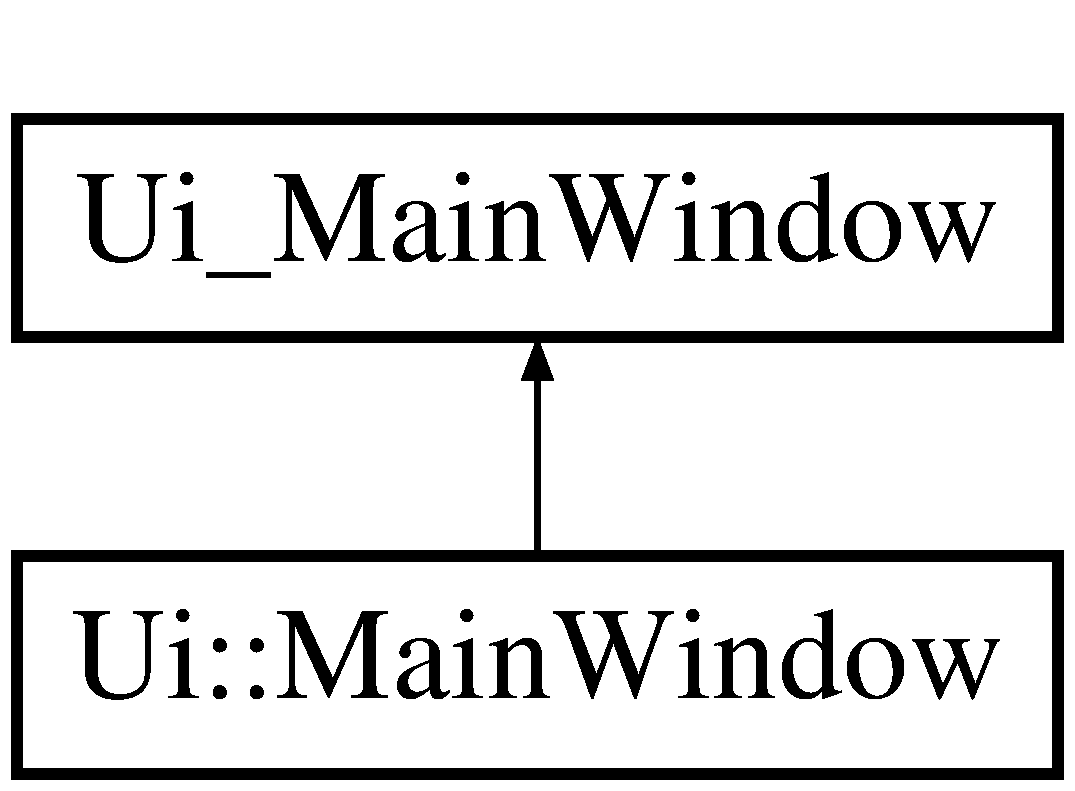
\includegraphics[height=2.000000cm]{class_ui___main_window}
\end{center}
\end{figure}
\subsection*{\-Public \-Member \-Functions}
\begin{DoxyCompactItemize}
\item 
void \hyperlink{class_ui___main_window_acf4a0872c4c77d8f43a2ec66ed849b58}{setup\-Ui} (\-Q\-Main\-Window $\ast$\-Main\-Window)
\item 
void \hyperlink{class_ui___main_window_a097dd160c3534a204904cb374412c618}{retranslate\-Ui} (\-Q\-Main\-Window $\ast$\-Main\-Window)
\end{DoxyCompactItemize}
\subsection*{\-Public \-Attributes}
\begin{DoxyCompactItemize}
\item 
\-Q\-Widget $\ast$ \hyperlink{class_ui___main_window_a30075506c2116c3ed4ff25e07ae75f81}{central\-Widget}
\item 
\-Q\-Grid\-Layout $\ast$ \hyperlink{class_ui___main_window_af42ea7d4c2e893181caad21e28166932}{grid\-Layout\-\_\-3}
\item 
\-Q\-Grid\-Layout $\ast$ \hyperlink{class_ui___main_window_a6b2a0c5f7e8ff2a87134908dd770d2d2}{grid\-Layout\-\_\-2}
\item 
\-Q\-H\-Box\-Layout $\ast$ \hyperlink{class_ui___main_window_acd6fdc9ebacc4b25b834162380d75ce8}{horizontal\-Layout}
\item 
\-Q\-Tool\-Button $\ast$ \hyperlink{class_ui___main_window_a9b4aced7d5563bf1ee62d944215a9a92}{play\-Button}
\item 
\-Q\-Tool\-Button $\ast$ \hyperlink{class_ui___main_window_adf0fe1ee3ae6e5766589c477c85ac16c}{pause\-Button}
\item 
\-Q\-Progress\-Bar $\ast$ \hyperlink{class_ui___main_window_a851cc4465d87a72d072b6559eb6b3a2a}{simulation\-Progress\-Bar}
\item 
\-Q\-Push\-Button $\ast$ \hyperlink{class_ui___main_window_ad332d93084584930878f1daf5f84cdbf}{push\-Button}
\item 
\-Q\-Grid\-Layout $\ast$ \hyperlink{class_ui___main_window_a525ed3c5fe0784ac502ee222fba4e205}{grid\-Layout}
\item 
\-Q\-Label $\ast$ \hyperlink{class_ui___main_window_aea754e8591e2a34ad9fd1b1a0d70a3ff}{\-N\-Cells}
\item 
\-Q\-Label $\ast$ \hyperlink{class_ui___main_window_a4f203fa20746d2f27d346c96a5ab9dd6}{\-N\-Cells\-Num}
\item 
\-Q\-Label $\ast$ \hyperlink{class_ui___main_window_a6b0d88d19ddcb52fec0cc1ed6a3e3d9c}{time}
\item 
\-Q\-Label $\ast$ \hyperlink{class_ui___main_window_a260f2ffc3170b0afd4162f5300f7153e}{time\-Num}
\item 
\-Q\-Label $\ast$ \hyperlink{class_ui___main_window_acb5251d8d9ed0c84133d2003a681dbce}{i\-Traj}
\item 
\-Q\-Label $\ast$ \hyperlink{class_ui___main_window_a48d251578b324caa31496795f0a1e678}{i\-Traj\-Num}
\item 
\-Q\-Label $\ast$ \hyperlink{class_ui___main_window_a4f1de3b858235bda33821eb68eb5a15b}{i\-Parameter\-Set}
\item 
\-Q\-Label $\ast$ \hyperlink{class_ui___main_window_a3f5d3def30871b917c64c2084368c320}{i\-Parameter\-Set\-Num}
\item 
\-Q\-V\-Box\-Layout $\ast$ \hyperlink{class_ui___main_window_aecd96a04789fcfec3f98d80390ad8184}{vertical\-Layout}
\item 
\-Q\-Group\-Box $\ast$ \hyperlink{class_ui___main_window_aef7cb3be8cecfc9aaf98f036a98781ce}{group\-Box}
\item 
\-Q\-H\-Box\-Layout $\ast$ \hyperlink{class_ui___main_window_a14c9d4842c3e97e16e7873ef0aecdb1e}{horizontal\-Layout\-\_\-5}
\item 
\-Q\-H\-Box\-Layout $\ast$ \hyperlink{class_ui___main_window_a80867018070156432923d0266cc9fe25}{horizontal\-Layout\-\_\-2}
\item 
\-Q\-Graphics\-View $\ast$ \hyperlink{class_ui___main_window_a9d358977cfd4428817e8ec8e76084d5a}{color\-Code\-Graphics\-View}
\item 
\-Q\-Double\-Spin\-Box $\ast$ \hyperlink{class_ui___main_window_a630d229a0c27bca9e8fa65c926ac9f82}{species\-Color\-Max\-Value\-Spin\-Box}
\item 
\-Q\-Combo\-Box $\ast$ \hyperlink{class_ui___main_window_a42def65165da6f0f6972d863ce6fe411}{species\-Color\-Combo\-Box}
\item 
\-Q\-Group\-Box $\ast$ \hyperlink{class_ui___main_window_abb28acde35ffce4d0e6152579df2cbc3}{group\-Box\-\_\-2}
\item 
\-Q\-H\-Box\-Layout $\ast$ \hyperlink{class_ui___main_window_ae183387a7d233b437a637b403ba39ffd}{horizontal\-Layout\-\_\-4}
\item 
\-Q\-H\-Box\-Layout $\ast$ \hyperlink{class_ui___main_window_a03ce63974cc69b067c91bbf285cceca8}{horizontal\-Layout\-\_\-3}
\item 
\-Q\-Graphics\-View $\ast$ \hyperlink{class_ui___main_window_a6514b2e16b9ea2f879bde5976b215e9b}{color\-Code\-Background\-Graphics\-View}
\item 
\-Q\-Double\-Spin\-Box $\ast$ \hyperlink{class_ui___main_window_a54a465855ecd4ab2fe51bdad8f2d0c81}{species\-Background\-Color\-Max\-Value\-Spin\-Box}
\item 
\-Q\-Combo\-Box $\ast$ \hyperlink{class_ui___main_window_ac3c8d5fa9d1ee6504fb0c77918c8e3bf}{species\-Background\-Color\-Combo\-Box}
\item 
\-Q\-Label $\ast$ \hyperlink{class_ui___main_window_a2e2516d755e4dd53fc905dabddf2738a}{label\-\_\-2}
\item 
\-Q\-Label $\ast$ \hyperlink{class_ui___main_window_a0376fd90247280e7c7957cc70628708c}{label\-\_\-3}
\item 
\-Q\-Table\-View $\ast$ \hyperlink{class_ui___main_window_a3baa50bd3a556afb670087812b6819a8}{global\-Parameter\-Table\-View}
\item 
\-Q\-Graphics\-View $\ast$ \hyperlink{class_ui___main_window_aadc961224465f9981b865ee8d392a34d}{colony\-View}
\item 
\-Q\-Table\-View $\ast$ \hyperlink{class_ui___main_window_af7f54d908065a273d04d5409dc2f81bf}{cell\-State\-Table\-View}
\item 
\-Q\-H\-Box\-Layout $\ast$ \hyperlink{class_ui___main_window_a1351e317cba7ca711b6b4d2212b6bf36}{horizontal\-Layout\-\_\-6}
\item 
\-Q\-Label $\ast$ \hyperlink{class_ui___main_window_ad9c89133780f28e6efa2ec17ceb9cff5}{label}
\item 
\-Q\-Slider $\ast$ \hyperlink{class_ui___main_window_a396d443a9748adbeed2928fce39034a2}{zoom\-Slider}
\item 
\-Q\-Tool\-Bar $\ast$ \hyperlink{class_ui___main_window_a5172877001c8c7b4e0f6de50421867d1}{main\-Tool\-Bar}
\item 
\-Q\-Status\-Bar $\ast$ \hyperlink{class_ui___main_window_a50fa481337604bcc8bf68de18ab16ecd}{status\-Bar}
\end{DoxyCompactItemize}


\subsection{\-Detailed \-Description}


\-Definition at line 38 of file ui\-\_\-mainwindow.\-h.



\subsection{\-Member \-Function \-Documentation}
\hypertarget{class_ui___main_window_a097dd160c3534a204904cb374412c618}{\index{\-Ui\-\_\-\-Main\-Window@{\-Ui\-\_\-\-Main\-Window}!retranslate\-Ui@{retranslate\-Ui}}
\index{retranslate\-Ui@{retranslate\-Ui}!Ui_MainWindow@{\-Ui\-\_\-\-Main\-Window}}
\subsubsection[{retranslate\-Ui}]{\setlength{\rightskip}{0pt plus 5cm}void {\bf \-Ui\-\_\-\-Main\-Window\-::retranslate\-Ui} (
\begin{DoxyParamCaption}
\item[{\-Q\-Main\-Window $\ast$}]{\-Main\-Window}
\end{DoxyParamCaption}
)\hspace{0.3cm}{\ttfamily  \mbox{[}inline\mbox{]}}}}\label{class_ui___main_window_a097dd160c3534a204904cb374412c618}


\-Definition at line 455 of file ui\-\_\-mainwindow.\-h.

\hypertarget{class_ui___main_window_acf4a0872c4c77d8f43a2ec66ed849b58}{\index{\-Ui\-\_\-\-Main\-Window@{\-Ui\-\_\-\-Main\-Window}!setup\-Ui@{setup\-Ui}}
\index{setup\-Ui@{setup\-Ui}!Ui_MainWindow@{\-Ui\-\_\-\-Main\-Window}}
\subsubsection[{setup\-Ui}]{\setlength{\rightskip}{0pt plus 5cm}void {\bf \-Ui\-\_\-\-Main\-Window\-::setup\-Ui} (
\begin{DoxyParamCaption}
\item[{\-Q\-Main\-Window $\ast$}]{\-Main\-Window}
\end{DoxyParamCaption}
)\hspace{0.3cm}{\ttfamily  \mbox{[}inline\mbox{]}}}}\label{class_ui___main_window_acf4a0872c4c77d8f43a2ec66ed849b58}


\-Definition at line 82 of file ui\-\_\-mainwindow.\-h.



\subsection{\-Member \-Data \-Documentation}
\hypertarget{class_ui___main_window_af7f54d908065a273d04d5409dc2f81bf}{\index{\-Ui\-\_\-\-Main\-Window@{\-Ui\-\_\-\-Main\-Window}!cell\-State\-Table\-View@{cell\-State\-Table\-View}}
\index{cell\-State\-Table\-View@{cell\-State\-Table\-View}!Ui_MainWindow@{\-Ui\-\_\-\-Main\-Window}}
\subsubsection[{cell\-State\-Table\-View}]{\setlength{\rightskip}{0pt plus 5cm}\-Q\-Table\-View$\ast$ {\bf \-Ui\-\_\-\-Main\-Window\-::cell\-State\-Table\-View}}}\label{class_ui___main_window_af7f54d908065a273d04d5409dc2f81bf}


\-Definition at line 75 of file ui\-\_\-mainwindow.\-h.

\hypertarget{class_ui___main_window_a30075506c2116c3ed4ff25e07ae75f81}{\index{\-Ui\-\_\-\-Main\-Window@{\-Ui\-\_\-\-Main\-Window}!central\-Widget@{central\-Widget}}
\index{central\-Widget@{central\-Widget}!Ui_MainWindow@{\-Ui\-\_\-\-Main\-Window}}
\subsubsection[{central\-Widget}]{\setlength{\rightskip}{0pt plus 5cm}\-Q\-Widget$\ast$ {\bf \-Ui\-\_\-\-Main\-Window\-::central\-Widget}}}\label{class_ui___main_window_a30075506c2116c3ed4ff25e07ae75f81}


\-Definition at line 41 of file ui\-\_\-mainwindow.\-h.

\hypertarget{class_ui___main_window_aadc961224465f9981b865ee8d392a34d}{\index{\-Ui\-\_\-\-Main\-Window@{\-Ui\-\_\-\-Main\-Window}!colony\-View@{colony\-View}}
\index{colony\-View@{colony\-View}!Ui_MainWindow@{\-Ui\-\_\-\-Main\-Window}}
\subsubsection[{colony\-View}]{\setlength{\rightskip}{0pt plus 5cm}\-Q\-Graphics\-View$\ast$ {\bf \-Ui\-\_\-\-Main\-Window\-::colony\-View}}}\label{class_ui___main_window_aadc961224465f9981b865ee8d392a34d}


\-Definition at line 74 of file ui\-\_\-mainwindow.\-h.

\hypertarget{class_ui___main_window_a6514b2e16b9ea2f879bde5976b215e9b}{\index{\-Ui\-\_\-\-Main\-Window@{\-Ui\-\_\-\-Main\-Window}!color\-Code\-Background\-Graphics\-View@{color\-Code\-Background\-Graphics\-View}}
\index{color\-Code\-Background\-Graphics\-View@{color\-Code\-Background\-Graphics\-View}!Ui_MainWindow@{\-Ui\-\_\-\-Main\-Window}}
\subsubsection[{color\-Code\-Background\-Graphics\-View}]{\setlength{\rightskip}{0pt plus 5cm}\-Q\-Graphics\-View$\ast$ {\bf \-Ui\-\_\-\-Main\-Window\-::color\-Code\-Background\-Graphics\-View}}}\label{class_ui___main_window_a6514b2e16b9ea2f879bde5976b215e9b}


\-Definition at line 68 of file ui\-\_\-mainwindow.\-h.

\hypertarget{class_ui___main_window_a9d358977cfd4428817e8ec8e76084d5a}{\index{\-Ui\-\_\-\-Main\-Window@{\-Ui\-\_\-\-Main\-Window}!color\-Code\-Graphics\-View@{color\-Code\-Graphics\-View}}
\index{color\-Code\-Graphics\-View@{color\-Code\-Graphics\-View}!Ui_MainWindow@{\-Ui\-\_\-\-Main\-Window}}
\subsubsection[{color\-Code\-Graphics\-View}]{\setlength{\rightskip}{0pt plus 5cm}\-Q\-Graphics\-View$\ast$ {\bf \-Ui\-\_\-\-Main\-Window\-::color\-Code\-Graphics\-View}}}\label{class_ui___main_window_a9d358977cfd4428817e8ec8e76084d5a}


\-Definition at line 62 of file ui\-\_\-mainwindow.\-h.

\hypertarget{class_ui___main_window_a3baa50bd3a556afb670087812b6819a8}{\index{\-Ui\-\_\-\-Main\-Window@{\-Ui\-\_\-\-Main\-Window}!global\-Parameter\-Table\-View@{global\-Parameter\-Table\-View}}
\index{global\-Parameter\-Table\-View@{global\-Parameter\-Table\-View}!Ui_MainWindow@{\-Ui\-\_\-\-Main\-Window}}
\subsubsection[{global\-Parameter\-Table\-View}]{\setlength{\rightskip}{0pt plus 5cm}\-Q\-Table\-View$\ast$ {\bf \-Ui\-\_\-\-Main\-Window\-::global\-Parameter\-Table\-View}}}\label{class_ui___main_window_a3baa50bd3a556afb670087812b6819a8}


\-Definition at line 73 of file ui\-\_\-mainwindow.\-h.

\hypertarget{class_ui___main_window_a525ed3c5fe0784ac502ee222fba4e205}{\index{\-Ui\-\_\-\-Main\-Window@{\-Ui\-\_\-\-Main\-Window}!grid\-Layout@{grid\-Layout}}
\index{grid\-Layout@{grid\-Layout}!Ui_MainWindow@{\-Ui\-\_\-\-Main\-Window}}
\subsubsection[{grid\-Layout}]{\setlength{\rightskip}{0pt plus 5cm}\-Q\-Grid\-Layout$\ast$ {\bf \-Ui\-\_\-\-Main\-Window\-::grid\-Layout}}}\label{class_ui___main_window_a525ed3c5fe0784ac502ee222fba4e205}


\-Definition at line 49 of file ui\-\_\-mainwindow.\-h.

\hypertarget{class_ui___main_window_a6b2a0c5f7e8ff2a87134908dd770d2d2}{\index{\-Ui\-\_\-\-Main\-Window@{\-Ui\-\_\-\-Main\-Window}!grid\-Layout\-\_\-2@{grid\-Layout\-\_\-2}}
\index{grid\-Layout\-\_\-2@{grid\-Layout\-\_\-2}!Ui_MainWindow@{\-Ui\-\_\-\-Main\-Window}}
\subsubsection[{grid\-Layout\-\_\-2}]{\setlength{\rightskip}{0pt plus 5cm}\-Q\-Grid\-Layout$\ast$ {\bf \-Ui\-\_\-\-Main\-Window\-::grid\-Layout\-\_\-2}}}\label{class_ui___main_window_a6b2a0c5f7e8ff2a87134908dd770d2d2}


\-Definition at line 43 of file ui\-\_\-mainwindow.\-h.

\hypertarget{class_ui___main_window_af42ea7d4c2e893181caad21e28166932}{\index{\-Ui\-\_\-\-Main\-Window@{\-Ui\-\_\-\-Main\-Window}!grid\-Layout\-\_\-3@{grid\-Layout\-\_\-3}}
\index{grid\-Layout\-\_\-3@{grid\-Layout\-\_\-3}!Ui_MainWindow@{\-Ui\-\_\-\-Main\-Window}}
\subsubsection[{grid\-Layout\-\_\-3}]{\setlength{\rightskip}{0pt plus 5cm}\-Q\-Grid\-Layout$\ast$ {\bf \-Ui\-\_\-\-Main\-Window\-::grid\-Layout\-\_\-3}}}\label{class_ui___main_window_af42ea7d4c2e893181caad21e28166932}


\-Definition at line 42 of file ui\-\_\-mainwindow.\-h.

\hypertarget{class_ui___main_window_aef7cb3be8cecfc9aaf98f036a98781ce}{\index{\-Ui\-\_\-\-Main\-Window@{\-Ui\-\_\-\-Main\-Window}!group\-Box@{group\-Box}}
\index{group\-Box@{group\-Box}!Ui_MainWindow@{\-Ui\-\_\-\-Main\-Window}}
\subsubsection[{group\-Box}]{\setlength{\rightskip}{0pt plus 5cm}\-Q\-Group\-Box$\ast$ {\bf \-Ui\-\_\-\-Main\-Window\-::group\-Box}}}\label{class_ui___main_window_aef7cb3be8cecfc9aaf98f036a98781ce}


\-Definition at line 59 of file ui\-\_\-mainwindow.\-h.

\hypertarget{class_ui___main_window_abb28acde35ffce4d0e6152579df2cbc3}{\index{\-Ui\-\_\-\-Main\-Window@{\-Ui\-\_\-\-Main\-Window}!group\-Box\-\_\-2@{group\-Box\-\_\-2}}
\index{group\-Box\-\_\-2@{group\-Box\-\_\-2}!Ui_MainWindow@{\-Ui\-\_\-\-Main\-Window}}
\subsubsection[{group\-Box\-\_\-2}]{\setlength{\rightskip}{0pt plus 5cm}\-Q\-Group\-Box$\ast$ {\bf \-Ui\-\_\-\-Main\-Window\-::group\-Box\-\_\-2}}}\label{class_ui___main_window_abb28acde35ffce4d0e6152579df2cbc3}


\-Definition at line 65 of file ui\-\_\-mainwindow.\-h.

\hypertarget{class_ui___main_window_acd6fdc9ebacc4b25b834162380d75ce8}{\index{\-Ui\-\_\-\-Main\-Window@{\-Ui\-\_\-\-Main\-Window}!horizontal\-Layout@{horizontal\-Layout}}
\index{horizontal\-Layout@{horizontal\-Layout}!Ui_MainWindow@{\-Ui\-\_\-\-Main\-Window}}
\subsubsection[{horizontal\-Layout}]{\setlength{\rightskip}{0pt plus 5cm}\-Q\-H\-Box\-Layout$\ast$ {\bf \-Ui\-\_\-\-Main\-Window\-::horizontal\-Layout}}}\label{class_ui___main_window_acd6fdc9ebacc4b25b834162380d75ce8}


\-Definition at line 44 of file ui\-\_\-mainwindow.\-h.

\hypertarget{class_ui___main_window_a80867018070156432923d0266cc9fe25}{\index{\-Ui\-\_\-\-Main\-Window@{\-Ui\-\_\-\-Main\-Window}!horizontal\-Layout\-\_\-2@{horizontal\-Layout\-\_\-2}}
\index{horizontal\-Layout\-\_\-2@{horizontal\-Layout\-\_\-2}!Ui_MainWindow@{\-Ui\-\_\-\-Main\-Window}}
\subsubsection[{horizontal\-Layout\-\_\-2}]{\setlength{\rightskip}{0pt plus 5cm}\-Q\-H\-Box\-Layout$\ast$ {\bf \-Ui\-\_\-\-Main\-Window\-::horizontal\-Layout\-\_\-2}}}\label{class_ui___main_window_a80867018070156432923d0266cc9fe25}


\-Definition at line 61 of file ui\-\_\-mainwindow.\-h.

\hypertarget{class_ui___main_window_a03ce63974cc69b067c91bbf285cceca8}{\index{\-Ui\-\_\-\-Main\-Window@{\-Ui\-\_\-\-Main\-Window}!horizontal\-Layout\-\_\-3@{horizontal\-Layout\-\_\-3}}
\index{horizontal\-Layout\-\_\-3@{horizontal\-Layout\-\_\-3}!Ui_MainWindow@{\-Ui\-\_\-\-Main\-Window}}
\subsubsection[{horizontal\-Layout\-\_\-3}]{\setlength{\rightskip}{0pt plus 5cm}\-Q\-H\-Box\-Layout$\ast$ {\bf \-Ui\-\_\-\-Main\-Window\-::horizontal\-Layout\-\_\-3}}}\label{class_ui___main_window_a03ce63974cc69b067c91bbf285cceca8}


\-Definition at line 67 of file ui\-\_\-mainwindow.\-h.

\hypertarget{class_ui___main_window_ae183387a7d233b437a637b403ba39ffd}{\index{\-Ui\-\_\-\-Main\-Window@{\-Ui\-\_\-\-Main\-Window}!horizontal\-Layout\-\_\-4@{horizontal\-Layout\-\_\-4}}
\index{horizontal\-Layout\-\_\-4@{horizontal\-Layout\-\_\-4}!Ui_MainWindow@{\-Ui\-\_\-\-Main\-Window}}
\subsubsection[{horizontal\-Layout\-\_\-4}]{\setlength{\rightskip}{0pt plus 5cm}\-Q\-H\-Box\-Layout$\ast$ {\bf \-Ui\-\_\-\-Main\-Window\-::horizontal\-Layout\-\_\-4}}}\label{class_ui___main_window_ae183387a7d233b437a637b403ba39ffd}


\-Definition at line 66 of file ui\-\_\-mainwindow.\-h.

\hypertarget{class_ui___main_window_a14c9d4842c3e97e16e7873ef0aecdb1e}{\index{\-Ui\-\_\-\-Main\-Window@{\-Ui\-\_\-\-Main\-Window}!horizontal\-Layout\-\_\-5@{horizontal\-Layout\-\_\-5}}
\index{horizontal\-Layout\-\_\-5@{horizontal\-Layout\-\_\-5}!Ui_MainWindow@{\-Ui\-\_\-\-Main\-Window}}
\subsubsection[{horizontal\-Layout\-\_\-5}]{\setlength{\rightskip}{0pt plus 5cm}\-Q\-H\-Box\-Layout$\ast$ {\bf \-Ui\-\_\-\-Main\-Window\-::horizontal\-Layout\-\_\-5}}}\label{class_ui___main_window_a14c9d4842c3e97e16e7873ef0aecdb1e}


\-Definition at line 60 of file ui\-\_\-mainwindow.\-h.

\hypertarget{class_ui___main_window_a1351e317cba7ca711b6b4d2212b6bf36}{\index{\-Ui\-\_\-\-Main\-Window@{\-Ui\-\_\-\-Main\-Window}!horizontal\-Layout\-\_\-6@{horizontal\-Layout\-\_\-6}}
\index{horizontal\-Layout\-\_\-6@{horizontal\-Layout\-\_\-6}!Ui_MainWindow@{\-Ui\-\_\-\-Main\-Window}}
\subsubsection[{horizontal\-Layout\-\_\-6}]{\setlength{\rightskip}{0pt plus 5cm}\-Q\-H\-Box\-Layout$\ast$ {\bf \-Ui\-\_\-\-Main\-Window\-::horizontal\-Layout\-\_\-6}}}\label{class_ui___main_window_a1351e317cba7ca711b6b4d2212b6bf36}


\-Definition at line 76 of file ui\-\_\-mainwindow.\-h.

\hypertarget{class_ui___main_window_a4f1de3b858235bda33821eb68eb5a15b}{\index{\-Ui\-\_\-\-Main\-Window@{\-Ui\-\_\-\-Main\-Window}!i\-Parameter\-Set@{i\-Parameter\-Set}}
\index{i\-Parameter\-Set@{i\-Parameter\-Set}!Ui_MainWindow@{\-Ui\-\_\-\-Main\-Window}}
\subsubsection[{i\-Parameter\-Set}]{\setlength{\rightskip}{0pt plus 5cm}\-Q\-Label$\ast$ {\bf \-Ui\-\_\-\-Main\-Window\-::i\-Parameter\-Set}}}\label{class_ui___main_window_a4f1de3b858235bda33821eb68eb5a15b}


\-Definition at line 56 of file ui\-\_\-mainwindow.\-h.

\hypertarget{class_ui___main_window_a3f5d3def30871b917c64c2084368c320}{\index{\-Ui\-\_\-\-Main\-Window@{\-Ui\-\_\-\-Main\-Window}!i\-Parameter\-Set\-Num@{i\-Parameter\-Set\-Num}}
\index{i\-Parameter\-Set\-Num@{i\-Parameter\-Set\-Num}!Ui_MainWindow@{\-Ui\-\_\-\-Main\-Window}}
\subsubsection[{i\-Parameter\-Set\-Num}]{\setlength{\rightskip}{0pt plus 5cm}\-Q\-Label$\ast$ {\bf \-Ui\-\_\-\-Main\-Window\-::i\-Parameter\-Set\-Num}}}\label{class_ui___main_window_a3f5d3def30871b917c64c2084368c320}


\-Definition at line 57 of file ui\-\_\-mainwindow.\-h.

\hypertarget{class_ui___main_window_acb5251d8d9ed0c84133d2003a681dbce}{\index{\-Ui\-\_\-\-Main\-Window@{\-Ui\-\_\-\-Main\-Window}!i\-Traj@{i\-Traj}}
\index{i\-Traj@{i\-Traj}!Ui_MainWindow@{\-Ui\-\_\-\-Main\-Window}}
\subsubsection[{i\-Traj}]{\setlength{\rightskip}{0pt plus 5cm}\-Q\-Label$\ast$ {\bf \-Ui\-\_\-\-Main\-Window\-::i\-Traj}}}\label{class_ui___main_window_acb5251d8d9ed0c84133d2003a681dbce}


\-Definition at line 54 of file ui\-\_\-mainwindow.\-h.

\hypertarget{class_ui___main_window_a48d251578b324caa31496795f0a1e678}{\index{\-Ui\-\_\-\-Main\-Window@{\-Ui\-\_\-\-Main\-Window}!i\-Traj\-Num@{i\-Traj\-Num}}
\index{i\-Traj\-Num@{i\-Traj\-Num}!Ui_MainWindow@{\-Ui\-\_\-\-Main\-Window}}
\subsubsection[{i\-Traj\-Num}]{\setlength{\rightskip}{0pt plus 5cm}\-Q\-Label$\ast$ {\bf \-Ui\-\_\-\-Main\-Window\-::i\-Traj\-Num}}}\label{class_ui___main_window_a48d251578b324caa31496795f0a1e678}


\-Definition at line 55 of file ui\-\_\-mainwindow.\-h.

\hypertarget{class_ui___main_window_ad9c89133780f28e6efa2ec17ceb9cff5}{\index{\-Ui\-\_\-\-Main\-Window@{\-Ui\-\_\-\-Main\-Window}!label@{label}}
\index{label@{label}!Ui_MainWindow@{\-Ui\-\_\-\-Main\-Window}}
\subsubsection[{label}]{\setlength{\rightskip}{0pt plus 5cm}\-Q\-Label$\ast$ {\bf \-Ui\-\_\-\-Main\-Window\-::label}}}\label{class_ui___main_window_ad9c89133780f28e6efa2ec17ceb9cff5}


\-Definition at line 77 of file ui\-\_\-mainwindow.\-h.

\hypertarget{class_ui___main_window_a2e2516d755e4dd53fc905dabddf2738a}{\index{\-Ui\-\_\-\-Main\-Window@{\-Ui\-\_\-\-Main\-Window}!label\-\_\-2@{label\-\_\-2}}
\index{label\-\_\-2@{label\-\_\-2}!Ui_MainWindow@{\-Ui\-\_\-\-Main\-Window}}
\subsubsection[{label\-\_\-2}]{\setlength{\rightskip}{0pt plus 5cm}\-Q\-Label$\ast$ {\bf \-Ui\-\_\-\-Main\-Window\-::label\-\_\-2}}}\label{class_ui___main_window_a2e2516d755e4dd53fc905dabddf2738a}


\-Definition at line 71 of file ui\-\_\-mainwindow.\-h.

\hypertarget{class_ui___main_window_a0376fd90247280e7c7957cc70628708c}{\index{\-Ui\-\_\-\-Main\-Window@{\-Ui\-\_\-\-Main\-Window}!label\-\_\-3@{label\-\_\-3}}
\index{label\-\_\-3@{label\-\_\-3}!Ui_MainWindow@{\-Ui\-\_\-\-Main\-Window}}
\subsubsection[{label\-\_\-3}]{\setlength{\rightskip}{0pt plus 5cm}\-Q\-Label$\ast$ {\bf \-Ui\-\_\-\-Main\-Window\-::label\-\_\-3}}}\label{class_ui___main_window_a0376fd90247280e7c7957cc70628708c}


\-Definition at line 72 of file ui\-\_\-mainwindow.\-h.

\hypertarget{class_ui___main_window_a5172877001c8c7b4e0f6de50421867d1}{\index{\-Ui\-\_\-\-Main\-Window@{\-Ui\-\_\-\-Main\-Window}!main\-Tool\-Bar@{main\-Tool\-Bar}}
\index{main\-Tool\-Bar@{main\-Tool\-Bar}!Ui_MainWindow@{\-Ui\-\_\-\-Main\-Window}}
\subsubsection[{main\-Tool\-Bar}]{\setlength{\rightskip}{0pt plus 5cm}\-Q\-Tool\-Bar$\ast$ {\bf \-Ui\-\_\-\-Main\-Window\-::main\-Tool\-Bar}}}\label{class_ui___main_window_a5172877001c8c7b4e0f6de50421867d1}


\-Definition at line 79 of file ui\-\_\-mainwindow.\-h.

\hypertarget{class_ui___main_window_aea754e8591e2a34ad9fd1b1a0d70a3ff}{\index{\-Ui\-\_\-\-Main\-Window@{\-Ui\-\_\-\-Main\-Window}!\-N\-Cells@{\-N\-Cells}}
\index{\-N\-Cells@{\-N\-Cells}!Ui_MainWindow@{\-Ui\-\_\-\-Main\-Window}}
\subsubsection[{\-N\-Cells}]{\setlength{\rightskip}{0pt plus 5cm}\-Q\-Label$\ast$ {\bf \-Ui\-\_\-\-Main\-Window\-::\-N\-Cells}}}\label{class_ui___main_window_aea754e8591e2a34ad9fd1b1a0d70a3ff}


\-Definition at line 50 of file ui\-\_\-mainwindow.\-h.

\hypertarget{class_ui___main_window_a4f203fa20746d2f27d346c96a5ab9dd6}{\index{\-Ui\-\_\-\-Main\-Window@{\-Ui\-\_\-\-Main\-Window}!\-N\-Cells\-Num@{\-N\-Cells\-Num}}
\index{\-N\-Cells\-Num@{\-N\-Cells\-Num}!Ui_MainWindow@{\-Ui\-\_\-\-Main\-Window}}
\subsubsection[{\-N\-Cells\-Num}]{\setlength{\rightskip}{0pt plus 5cm}\-Q\-Label$\ast$ {\bf \-Ui\-\_\-\-Main\-Window\-::\-N\-Cells\-Num}}}\label{class_ui___main_window_a4f203fa20746d2f27d346c96a5ab9dd6}


\-Definition at line 51 of file ui\-\_\-mainwindow.\-h.

\hypertarget{class_ui___main_window_adf0fe1ee3ae6e5766589c477c85ac16c}{\index{\-Ui\-\_\-\-Main\-Window@{\-Ui\-\_\-\-Main\-Window}!pause\-Button@{pause\-Button}}
\index{pause\-Button@{pause\-Button}!Ui_MainWindow@{\-Ui\-\_\-\-Main\-Window}}
\subsubsection[{pause\-Button}]{\setlength{\rightskip}{0pt plus 5cm}\-Q\-Tool\-Button$\ast$ {\bf \-Ui\-\_\-\-Main\-Window\-::pause\-Button}}}\label{class_ui___main_window_adf0fe1ee3ae6e5766589c477c85ac16c}


\-Definition at line 46 of file ui\-\_\-mainwindow.\-h.

\hypertarget{class_ui___main_window_a9b4aced7d5563bf1ee62d944215a9a92}{\index{\-Ui\-\_\-\-Main\-Window@{\-Ui\-\_\-\-Main\-Window}!play\-Button@{play\-Button}}
\index{play\-Button@{play\-Button}!Ui_MainWindow@{\-Ui\-\_\-\-Main\-Window}}
\subsubsection[{play\-Button}]{\setlength{\rightskip}{0pt plus 5cm}\-Q\-Tool\-Button$\ast$ {\bf \-Ui\-\_\-\-Main\-Window\-::play\-Button}}}\label{class_ui___main_window_a9b4aced7d5563bf1ee62d944215a9a92}


\-Definition at line 45 of file ui\-\_\-mainwindow.\-h.

\hypertarget{class_ui___main_window_ad332d93084584930878f1daf5f84cdbf}{\index{\-Ui\-\_\-\-Main\-Window@{\-Ui\-\_\-\-Main\-Window}!push\-Button@{push\-Button}}
\index{push\-Button@{push\-Button}!Ui_MainWindow@{\-Ui\-\_\-\-Main\-Window}}
\subsubsection[{push\-Button}]{\setlength{\rightskip}{0pt plus 5cm}\-Q\-Push\-Button$\ast$ {\bf \-Ui\-\_\-\-Main\-Window\-::push\-Button}}}\label{class_ui___main_window_ad332d93084584930878f1daf5f84cdbf}


\-Definition at line 48 of file ui\-\_\-mainwindow.\-h.

\hypertarget{class_ui___main_window_a851cc4465d87a72d072b6559eb6b3a2a}{\index{\-Ui\-\_\-\-Main\-Window@{\-Ui\-\_\-\-Main\-Window}!simulation\-Progress\-Bar@{simulation\-Progress\-Bar}}
\index{simulation\-Progress\-Bar@{simulation\-Progress\-Bar}!Ui_MainWindow@{\-Ui\-\_\-\-Main\-Window}}
\subsubsection[{simulation\-Progress\-Bar}]{\setlength{\rightskip}{0pt plus 5cm}\-Q\-Progress\-Bar$\ast$ {\bf \-Ui\-\_\-\-Main\-Window\-::simulation\-Progress\-Bar}}}\label{class_ui___main_window_a851cc4465d87a72d072b6559eb6b3a2a}


\-Definition at line 47 of file ui\-\_\-mainwindow.\-h.

\hypertarget{class_ui___main_window_ac3c8d5fa9d1ee6504fb0c77918c8e3bf}{\index{\-Ui\-\_\-\-Main\-Window@{\-Ui\-\_\-\-Main\-Window}!species\-Background\-Color\-Combo\-Box@{species\-Background\-Color\-Combo\-Box}}
\index{species\-Background\-Color\-Combo\-Box@{species\-Background\-Color\-Combo\-Box}!Ui_MainWindow@{\-Ui\-\_\-\-Main\-Window}}
\subsubsection[{species\-Background\-Color\-Combo\-Box}]{\setlength{\rightskip}{0pt plus 5cm}\-Q\-Combo\-Box$\ast$ {\bf \-Ui\-\_\-\-Main\-Window\-::species\-Background\-Color\-Combo\-Box}}}\label{class_ui___main_window_ac3c8d5fa9d1ee6504fb0c77918c8e3bf}


\-Definition at line 70 of file ui\-\_\-mainwindow.\-h.

\hypertarget{class_ui___main_window_a54a465855ecd4ab2fe51bdad8f2d0c81}{\index{\-Ui\-\_\-\-Main\-Window@{\-Ui\-\_\-\-Main\-Window}!species\-Background\-Color\-Max\-Value\-Spin\-Box@{species\-Background\-Color\-Max\-Value\-Spin\-Box}}
\index{species\-Background\-Color\-Max\-Value\-Spin\-Box@{species\-Background\-Color\-Max\-Value\-Spin\-Box}!Ui_MainWindow@{\-Ui\-\_\-\-Main\-Window}}
\subsubsection[{species\-Background\-Color\-Max\-Value\-Spin\-Box}]{\setlength{\rightskip}{0pt plus 5cm}\-Q\-Double\-Spin\-Box$\ast$ {\bf \-Ui\-\_\-\-Main\-Window\-::species\-Background\-Color\-Max\-Value\-Spin\-Box}}}\label{class_ui___main_window_a54a465855ecd4ab2fe51bdad8f2d0c81}


\-Definition at line 69 of file ui\-\_\-mainwindow.\-h.

\hypertarget{class_ui___main_window_a42def65165da6f0f6972d863ce6fe411}{\index{\-Ui\-\_\-\-Main\-Window@{\-Ui\-\_\-\-Main\-Window}!species\-Color\-Combo\-Box@{species\-Color\-Combo\-Box}}
\index{species\-Color\-Combo\-Box@{species\-Color\-Combo\-Box}!Ui_MainWindow@{\-Ui\-\_\-\-Main\-Window}}
\subsubsection[{species\-Color\-Combo\-Box}]{\setlength{\rightskip}{0pt plus 5cm}\-Q\-Combo\-Box$\ast$ {\bf \-Ui\-\_\-\-Main\-Window\-::species\-Color\-Combo\-Box}}}\label{class_ui___main_window_a42def65165da6f0f6972d863ce6fe411}


\-Definition at line 64 of file ui\-\_\-mainwindow.\-h.

\hypertarget{class_ui___main_window_a630d229a0c27bca9e8fa65c926ac9f82}{\index{\-Ui\-\_\-\-Main\-Window@{\-Ui\-\_\-\-Main\-Window}!species\-Color\-Max\-Value\-Spin\-Box@{species\-Color\-Max\-Value\-Spin\-Box}}
\index{species\-Color\-Max\-Value\-Spin\-Box@{species\-Color\-Max\-Value\-Spin\-Box}!Ui_MainWindow@{\-Ui\-\_\-\-Main\-Window}}
\subsubsection[{species\-Color\-Max\-Value\-Spin\-Box}]{\setlength{\rightskip}{0pt plus 5cm}\-Q\-Double\-Spin\-Box$\ast$ {\bf \-Ui\-\_\-\-Main\-Window\-::species\-Color\-Max\-Value\-Spin\-Box}}}\label{class_ui___main_window_a630d229a0c27bca9e8fa65c926ac9f82}


\-Definition at line 63 of file ui\-\_\-mainwindow.\-h.

\hypertarget{class_ui___main_window_a50fa481337604bcc8bf68de18ab16ecd}{\index{\-Ui\-\_\-\-Main\-Window@{\-Ui\-\_\-\-Main\-Window}!status\-Bar@{status\-Bar}}
\index{status\-Bar@{status\-Bar}!Ui_MainWindow@{\-Ui\-\_\-\-Main\-Window}}
\subsubsection[{status\-Bar}]{\setlength{\rightskip}{0pt plus 5cm}\-Q\-Status\-Bar$\ast$ {\bf \-Ui\-\_\-\-Main\-Window\-::status\-Bar}}}\label{class_ui___main_window_a50fa481337604bcc8bf68de18ab16ecd}


\-Definition at line 80 of file ui\-\_\-mainwindow.\-h.

\hypertarget{class_ui___main_window_a6b0d88d19ddcb52fec0cc1ed6a3e3d9c}{\index{\-Ui\-\_\-\-Main\-Window@{\-Ui\-\_\-\-Main\-Window}!time@{time}}
\index{time@{time}!Ui_MainWindow@{\-Ui\-\_\-\-Main\-Window}}
\subsubsection[{time}]{\setlength{\rightskip}{0pt plus 5cm}\-Q\-Label$\ast$ {\bf \-Ui\-\_\-\-Main\-Window\-::time}}}\label{class_ui___main_window_a6b0d88d19ddcb52fec0cc1ed6a3e3d9c}


\-Definition at line 52 of file ui\-\_\-mainwindow.\-h.

\hypertarget{class_ui___main_window_a260f2ffc3170b0afd4162f5300f7153e}{\index{\-Ui\-\_\-\-Main\-Window@{\-Ui\-\_\-\-Main\-Window}!time\-Num@{time\-Num}}
\index{time\-Num@{time\-Num}!Ui_MainWindow@{\-Ui\-\_\-\-Main\-Window}}
\subsubsection[{time\-Num}]{\setlength{\rightskip}{0pt plus 5cm}\-Q\-Label$\ast$ {\bf \-Ui\-\_\-\-Main\-Window\-::time\-Num}}}\label{class_ui___main_window_a260f2ffc3170b0afd4162f5300f7153e}


\-Definition at line 53 of file ui\-\_\-mainwindow.\-h.

\hypertarget{class_ui___main_window_aecd96a04789fcfec3f98d80390ad8184}{\index{\-Ui\-\_\-\-Main\-Window@{\-Ui\-\_\-\-Main\-Window}!vertical\-Layout@{vertical\-Layout}}
\index{vertical\-Layout@{vertical\-Layout}!Ui_MainWindow@{\-Ui\-\_\-\-Main\-Window}}
\subsubsection[{vertical\-Layout}]{\setlength{\rightskip}{0pt plus 5cm}\-Q\-V\-Box\-Layout$\ast$ {\bf \-Ui\-\_\-\-Main\-Window\-::vertical\-Layout}}}\label{class_ui___main_window_aecd96a04789fcfec3f98d80390ad8184}


\-Definition at line 58 of file ui\-\_\-mainwindow.\-h.

\hypertarget{class_ui___main_window_a396d443a9748adbeed2928fce39034a2}{\index{\-Ui\-\_\-\-Main\-Window@{\-Ui\-\_\-\-Main\-Window}!zoom\-Slider@{zoom\-Slider}}
\index{zoom\-Slider@{zoom\-Slider}!Ui_MainWindow@{\-Ui\-\_\-\-Main\-Window}}
\subsubsection[{zoom\-Slider}]{\setlength{\rightskip}{0pt plus 5cm}\-Q\-Slider$\ast$ {\bf \-Ui\-\_\-\-Main\-Window\-::zoom\-Slider}}}\label{class_ui___main_window_a396d443a9748adbeed2928fce39034a2}


\-Definition at line 78 of file ui\-\_\-mainwindow.\-h.



\-The documentation for this class was generated from the following file\-:\begin{DoxyCompactItemize}
\item 
/media/\-My\-Passport\-Blue/\-Data/\-Research/\-Simulations/\-Colony/\hyperlink{ui__mainwindow_8h}{ui\-\_\-mainwindow.\-h}\end{DoxyCompactItemize}

\chapter{\-File \-Documentation}
\hypertarget{app_8cpp}{\section{/media/\-My\-Passport\-Blue/\-Data/\-Research/\-Simulations/\-Colony/app.cpp \-File \-Reference}
\label{app_8cpp}\index{/media/\-My\-Passport\-Blue/\-Data/\-Research/\-Simulations/\-Colony/app.\-cpp@{/media/\-My\-Passport\-Blue/\-Data/\-Research/\-Simulations/\-Colony/app.\-cpp}}
}
{\ttfamily \#include \char`\"{}debug.\-h\char`\"{}}\*
{\ttfamily \#include $<$iostream$>$}\*
{\ttfamily \#include $<$iomanip$>$}\*
{\ttfamily \#include $<$utility$>$}\*
{\ttfamily \#include $<$blitz/array.\-h$>$}\*
{\ttfamily \#include \char`\"{}\-Simulator.\-h\char`\"{}}\*
\subsection*{\-Functions}
\begin{DoxyCompactItemize}
\item 
int \hyperlink{app_8cpp_ae66f6b31b5ad750f1fe042a706a4e3d4}{main} ()
\end{DoxyCompactItemize}


\subsection{\-Detailed \-Description}
\-Project\-: \-Colony

\begin{DoxyAuthor}{\-Author}
\-Marc \-Weber\par
 \-The \-Si.\-M.\-Bio.\-Sys. \-Group (\-Cosmo\-Lab)\par
 \-Parc \-Científic de \-Barcelona\par
 \-Barcelona, \-Spain.\par
 \href{http://thesimbiosys.isgreat.org}{\tt http\-://thesimbiosys.\-isgreat.\-org} 
\end{DoxyAuthor}
\begin{DoxyVersion}{\-Version}
0.\-1 
\end{DoxyVersion}
\begin{DoxyDate}{\-Date}
11/2009
\end{DoxyDate}
\-Copyright 2009 by \-Marc \-Weber 

\-Definition in file \hyperlink{app_8cpp_source}{app.\-cpp}.



\subsection{\-Function \-Documentation}
\hypertarget{app_8cpp_ae66f6b31b5ad750f1fe042a706a4e3d4}{\index{app.\-cpp@{app.\-cpp}!main@{main}}
\index{main@{main}!app.cpp@{app.\-cpp}}
\subsubsection[{main}]{\setlength{\rightskip}{0pt plus 5cm}int {\bf main} (
\begin{DoxyParamCaption}
{}
\end{DoxyParamCaption}
)}}\label{app_8cpp_ae66f6b31b5ad750f1fe042a706a4e3d4}


\-Definition at line 39 of file app.\-cpp.


\hypertarget{apptest_8cpp}{\section{/media/\-My\-Passport\-Blue/\-Data/\-Research/\-Simulations/\-Colony/apptest.cpp \-File \-Reference}
\label{apptest_8cpp}\index{/media/\-My\-Passport\-Blue/\-Data/\-Research/\-Simulations/\-Colony/apptest.\-cpp@{/media/\-My\-Passport\-Blue/\-Data/\-Research/\-Simulations/\-Colony/apptest.\-cpp}}
}
{\ttfamily \#include \char`\"{}debug.\-h\char`\"{}}\*
{\ttfamily \#include $<$iostream$>$}\*
{\ttfamily \#include $<$iomanip$>$}\*
{\ttfamily \#include $<$utility$>$}\*
{\ttfamily \#include $<$blitz/array.\-h$>$}\*
{\ttfamily \#include \char`\"{}\-Simulator.\-h\char`\"{}}\*
\subsection*{\-Defines}
\begin{DoxyCompactItemize}
\item 
\#define \hyperlink{apptest_8cpp_a62953d5c052a6e06ae51712a315052f8}{\-D\-E\-B\-U\-G\-\_\-\-S\-I\-M\-U\-L\-A\-T\-O\-R\-\_\-\-N\-T\-R\-A\-J}
\end{DoxyCompactItemize}
\subsection*{\-Functions}
\begin{DoxyCompactItemize}
\item 
int \hyperlink{apptest_8cpp_ae66f6b31b5ad750f1fe042a706a4e3d4}{main} ()
\end{DoxyCompactItemize}


\subsection{\-Detailed \-Description}
\-Project\-: \-Colony

\begin{DoxyAuthor}{\-Author}
\-Marc \-Weber\par
 \-The \-Si.\-M.\-Bio.\-Sys. \-Group (\-Cosmo\-Lab)\par
 \-Parc \-Científic de \-Barcelona\par
 \-Barcelona, \-Spain.\par
 \href{http://thesimbiosys.isgreat.org}{\tt http\-://thesimbiosys.\-isgreat.\-org} 
\end{DoxyAuthor}
\begin{DoxyVersion}{\-Version}
0.\-1 
\end{DoxyVersion}
\begin{DoxyDate}{\-Date}
11/2009
\end{DoxyDate}
\-Copyright 2009 by \-Marc \-Weber 

\-Definition in file \hyperlink{apptest_8cpp_source}{apptest.\-cpp}.



\subsection{\-Define \-Documentation}
\hypertarget{apptest_8cpp_a62953d5c052a6e06ae51712a315052f8}{\index{apptest.\-cpp@{apptest.\-cpp}!\-D\-E\-B\-U\-G\-\_\-\-S\-I\-M\-U\-L\-A\-T\-O\-R\-\_\-\-N\-T\-R\-A\-J@{\-D\-E\-B\-U\-G\-\_\-\-S\-I\-M\-U\-L\-A\-T\-O\-R\-\_\-\-N\-T\-R\-A\-J}}
\index{\-D\-E\-B\-U\-G\-\_\-\-S\-I\-M\-U\-L\-A\-T\-O\-R\-\_\-\-N\-T\-R\-A\-J@{\-D\-E\-B\-U\-G\-\_\-\-S\-I\-M\-U\-L\-A\-T\-O\-R\-\_\-\-N\-T\-R\-A\-J}!apptest.cpp@{apptest.\-cpp}}
\subsubsection[{\-D\-E\-B\-U\-G\-\_\-\-S\-I\-M\-U\-L\-A\-T\-O\-R\-\_\-\-N\-T\-R\-A\-J}]{\setlength{\rightskip}{0pt plus 5cm}\#define {\bf \-D\-E\-B\-U\-G\-\_\-\-S\-I\-M\-U\-L\-A\-T\-O\-R\-\_\-\-N\-T\-R\-A\-J}}}\label{apptest_8cpp_a62953d5c052a6e06ae51712a315052f8}


\subsection{\-Function \-Documentation}
\hypertarget{apptest_8cpp_ae66f6b31b5ad750f1fe042a706a4e3d4}{\index{apptest.\-cpp@{apptest.\-cpp}!main@{main}}
\index{main@{main}!apptest.cpp@{apptest.\-cpp}}
\subsubsection[{main}]{\setlength{\rightskip}{0pt plus 5cm}int {\bf main} (
\begin{DoxyParamCaption}
{}
\end{DoxyParamCaption}
)}}\label{apptest_8cpp_ae66f6b31b5ad750f1fe042a706a4e3d4}


\-Definition at line 39 of file apptest.\-cpp.


\hypertarget{_cell_8cpp}{\section{/media/\-My\-Passport\-Blue/\-Data/\-Research/\-Simulations/\-Colony/\-Cell.cpp \-File \-Reference}
\label{_cell_8cpp}\index{/media/\-My\-Passport\-Blue/\-Data/\-Research/\-Simulations/\-Colony/\-Cell.\-cpp@{/media/\-My\-Passport\-Blue/\-Data/\-Research/\-Simulations/\-Colony/\-Cell.\-cpp}}
}
{\ttfamily \#include \char`\"{}\-Cell.\-h\char`\"{}}\*
\subsection*{\-Functions}
\begin{DoxyCompactItemize}
\item 
ostream \& \hyperlink{_cell_8cpp_ab7519ad9f97e822bc4c886ea1e85c29f}{operator$<$$<$} (ostream \&out, const \hyperlink{class_cell}{\-Cell} \&c)
\end{DoxyCompactItemize}


\subsection{\-Detailed \-Description}
\-Project\-: \-Colony

\begin{DoxyAuthor}{\-Author}
\-Marc \-Weber\par
 \-The \-Si\-M\-Bio\-Sys group (\-Cosmo\-Lab)\par
 \-Parc \-Científic de \-Barcelona\par
 \-Barcelona, \-Spain.\par
 \href{http://www.thesimbiosys.com}{\tt http\-://www.\-thesimbiosys.\-com} 
\end{DoxyAuthor}
\begin{DoxyVersion}{\-Version}
1.\-0 
\end{DoxyVersion}
\begin{DoxyDate}{\-Date}
11/2009
\end{DoxyDate}
\-Copyright 2009 by \-Marc \-Weber 

\-Definition in file \hyperlink{_cell_8cpp_source}{\-Cell.\-cpp}.



\subsection{\-Function \-Documentation}
\hypertarget{_cell_8cpp_ab7519ad9f97e822bc4c886ea1e85c29f}{\index{\-Cell.\-cpp@{\-Cell.\-cpp}!operator$<$$<$@{operator$<$$<$}}
\index{operator$<$$<$@{operator$<$$<$}!Cell.cpp@{\-Cell.\-cpp}}
\subsubsection[{operator$<$$<$}]{\setlength{\rightskip}{0pt plus 5cm}ostream\& operator$<$$<$ (
\begin{DoxyParamCaption}
\item[{ostream \&}]{out, }
\item[{const {\bf \-Cell} \&}]{c}
\end{DoxyParamCaption}
)}}\label{_cell_8cpp_ab7519ad9f97e822bc4c886ea1e85c29f}
\-Operator that outputs the content of a \hyperlink{class_cell}{\-Cell} state. \-Remark\-: it is declared as a friend operator, so that it has access to the private part of the \hyperlink{class_cell}{\-Cell} class. \-Overloading the $<$$<$ operator of class \hyperlink{class_cell_base}{\-Cell\-Base}. 

\-Definition at line 176 of file \-Cell.\-cpp.


\hypertarget{_cell_8h}{\section{/media/\-My\-Passport\-Blue/\-Data/\-Research/\-Simulations/\-Colony/\-Cell.h \-File \-Reference}
\label{_cell_8h}\index{/media/\-My\-Passport\-Blue/\-Data/\-Research/\-Simulations/\-Colony/\-Cell.\-h@{/media/\-My\-Passport\-Blue/\-Data/\-Research/\-Simulations/\-Colony/\-Cell.\-h}}
}
{\ttfamily \#include \char`\"{}debug.\-h\char`\"{}}\*
{\ttfamily \#include $<$vector$>$}\*
{\ttfamily \#include $<$string$>$}\*
{\ttfamily \#include $<$blitz/array.\-h$>$}\*
{\ttfamily \#include \char`\"{}\-Cell\-Base.\-h\char`\"{}}\*
{\ttfamily \#include \char`\"{}\-Graphics\-Cell\-Composite.\-h\char`\"{}}\*
{\ttfamily \#include \char`\"{}\-Cell\-Milieu\-Chemical\-System.\-h\char`\"{}}\*
{\ttfamily \#include \char`\"{}\-Random\-Number\-Generator.\-h\char`\"{}}\*
{\ttfamily \#include \char`\"{}\-Param/\-Cell\-Init\-Param.\-h\char`\"{}}\*
\subsection*{\-Classes}
\begin{DoxyCompactItemize}
\item 
class \hyperlink{class_cell}{\-Cell}
\end{DoxyCompactItemize}


\subsection{\-Detailed \-Description}
\-Project\-: \-Colony

\begin{DoxyAuthor}{\-Author}
\-Marc \-Weber\par
 \-The \-Si\-M\-Bio\-Sys group (\-Cosmo\-Lab)\par
 \-Parc \-Científic de \-Barcelona\par
 \-Barcelona, \-Spain.\par
 \href{http://www.thesimbiosys.com}{\tt http\-://www.\-thesimbiosys.\-com} 
\end{DoxyAuthor}
\begin{DoxyVersion}{\-Version}
1.\-0 
\end{DoxyVersion}
\begin{DoxyDate}{\-Date}
11/2009
\end{DoxyDate}
\-Copyright 2009 by \-Marc \-Weber 

\-Definition in file \hyperlink{_cell_8h_source}{\-Cell.\-h}.


\hypertarget{_cell_base_8cpp}{\section{/media/\-My\-Passport\-Blue/\-Data/\-Research/\-Simulations/\-Colony/\-Cell\-Base.cpp \-File \-Reference}
\label{_cell_base_8cpp}\index{/media/\-My\-Passport\-Blue/\-Data/\-Research/\-Simulations/\-Colony/\-Cell\-Base.\-cpp@{/media/\-My\-Passport\-Blue/\-Data/\-Research/\-Simulations/\-Colony/\-Cell\-Base.\-cpp}}
}
{\ttfamily \#include \char`\"{}\-Cell\-Base.\-h\char`\"{}}\*
\subsection*{\-Functions}
\begin{DoxyCompactItemize}
\item 
ostream \& \hyperlink{_cell_base_8cpp_ad3061d9b136ee7884ff7c255a977fd78}{operator$<$$<$} (ostream \&out, const \hyperlink{class_cell_base}{\-Cell\-Base} \&c)
\end{DoxyCompactItemize}


\subsection{\-Detailed \-Description}
\-Project\-: \-Colony

\begin{DoxyAuthor}{\-Author}
\-Marc \-Weber\par
 \-The \-Si\-M\-Bio\-Sys group (\-Cosmo\-Lab)\par
 \-Parc \-Científic de \-Barcelona\par
 \-Barcelona, \-Spain.\par
 \href{http://www.thesimbiosys.com}{\tt http\-://www.\-thesimbiosys.\-com} 
\end{DoxyAuthor}
\begin{DoxyVersion}{\-Version}
1.\-0 
\end{DoxyVersion}
\begin{DoxyDate}{\-Date}
11/2009
\end{DoxyDate}
\-Copyright 2009 by \-Marc \-Weber 

\-Definition in file \hyperlink{_cell_base_8cpp_source}{\-Cell\-Base.\-cpp}.



\subsection{\-Function \-Documentation}
\hypertarget{_cell_base_8cpp_ad3061d9b136ee7884ff7c255a977fd78}{\index{\-Cell\-Base.\-cpp@{\-Cell\-Base.\-cpp}!operator$<$$<$@{operator$<$$<$}}
\index{operator$<$$<$@{operator$<$$<$}!CellBase.cpp@{\-Cell\-Base.\-cpp}}
\subsubsection[{operator$<$$<$}]{\setlength{\rightskip}{0pt plus 5cm}ostream\& operator$<$$<$ (
\begin{DoxyParamCaption}
\item[{ostream \&}]{out, }
\item[{const {\bf \-Cell\-Base} \&}]{c}
\end{DoxyParamCaption}
)}}\label{_cell_base_8cpp_ad3061d9b136ee7884ff7c255a977fd78}
\-Operator that outputs the content of a \hyperlink{class_cell}{\-Cell} state. \-Remark\-: it is declared as a friend operator, so that it has access to the private part of the \hyperlink{class_cell_base}{\-Cell\-Base} class. 

\-Definition at line 71 of file \-Cell\-Base.\-cpp.


\hypertarget{_cell_base_8h}{\section{/media/\-My\-Passport\-Blue/\-Data/\-Research/\-Simulations/\-Colony/\-Cell\-Base.h \-File \-Reference}
\label{_cell_base_8h}\index{/media/\-My\-Passport\-Blue/\-Data/\-Research/\-Simulations/\-Colony/\-Cell\-Base.\-h@{/media/\-My\-Passport\-Blue/\-Data/\-Research/\-Simulations/\-Colony/\-Cell\-Base.\-h}}
}
{\ttfamily \#include \char`\"{}debug.\-h\char`\"{}}\*
{\ttfamily \#include $<$iostream$>$}\*
{\ttfamily \#include $<$vector$>$}\*
{\ttfamily \#include $<$string$>$}\*
{\ttfamily \#include $<$blitz/array.\-h$>$}\*
{\ttfamily \#include \char`\"{}\-State.\-h\char`\"{}}\*
{\ttfamily \#include \char`\"{}\-Chemical\-System.\-h\char`\"{}}\*
{\ttfamily \#include \char`\"{}\-Random\-Number\-Generator.\-h\char`\"{}}\*
{\ttfamily \#include \char`\"{}\-Param/\-Cell\-Base\-Init\-Param.\-h\char`\"{}}\*
\subsection*{\-Classes}
\begin{DoxyCompactItemize}
\item 
class \hyperlink{class_cell_base}{\-Cell\-Base}
\end{DoxyCompactItemize}


\subsection{\-Detailed \-Description}
\-Project\-: \-Colony

\begin{DoxyAuthor}{\-Author}
\-Marc \-Weber\par
 \-The \-Si\-M\-Bio\-Sys group (\-Cosmo\-Lab)\par
 \-Parc \-Científic de \-Barcelona\par
 \-Barcelona, \-Spain.\par
 \href{http://www.thesimbiosys.com}{\tt http\-://www.\-thesimbiosys.\-com} 
\end{DoxyAuthor}
\begin{DoxyVersion}{\-Version}
1.\-0 
\end{DoxyVersion}
\begin{DoxyDate}{\-Date}
11/2009
\end{DoxyDate}
\-Copyright 2009 by \-Marc \-Weber 

\-Definition in file \hyperlink{_cell_base_8h_source}{\-Cell\-Base.\-h}.


\hypertarget{_cell_collection_8cpp}{\section{/media/\-My\-Passport\-Blue/\-Data/\-Research/\-Simulations/\-Colony/\-Cell\-Collection.cpp \-File \-Reference}
\label{_cell_collection_8cpp}\index{/media/\-My\-Passport\-Blue/\-Data/\-Research/\-Simulations/\-Colony/\-Cell\-Collection.\-cpp@{/media/\-My\-Passport\-Blue/\-Data/\-Research/\-Simulations/\-Colony/\-Cell\-Collection.\-cpp}}
}
{\ttfamily \#include \char`\"{}\-Cell\-Collection.\-h\char`\"{}}\*
\subsection*{\-Functions}
\begin{DoxyCompactItemize}
\item 
ostream \& \hyperlink{_cell_collection_8cpp_ab0a78cc0f31cec81458f40ab27bc7beb}{operator$<$$<$} (ostream \&out, const \hyperlink{class_cell_collection}{\-Cell\-Collection} \&cell\-Collection)
\end{DoxyCompactItemize}


\subsection{\-Detailed \-Description}
\-Project\-: \-Colony

\begin{DoxyAuthor}{\-Author}
\-Marc \-Weber\par
 \-The \-Si\-M\-Bio\-Sys group (\-Cosmo\-Lab)\par
 \-Parc \-Científic de \-Barcelona\par
 \-Barcelona, \-Spain.\par
 \href{http://www.thesimbiosys.com}{\tt http\-://www.\-thesimbiosys.\-com} 
\end{DoxyAuthor}
\begin{DoxyVersion}{\-Version}
1.\-0 
\end{DoxyVersion}
\begin{DoxyDate}{\-Date}
11/2009
\end{DoxyDate}
\-Copyright 2009 by \-Marc \-Weber 

\-Definition in file \hyperlink{_cell_collection_8cpp_source}{\-Cell\-Collection.\-cpp}.



\subsection{\-Function \-Documentation}
\hypertarget{_cell_collection_8cpp_ab0a78cc0f31cec81458f40ab27bc7beb}{\index{\-Cell\-Collection.\-cpp@{\-Cell\-Collection.\-cpp}!operator$<$$<$@{operator$<$$<$}}
\index{operator$<$$<$@{operator$<$$<$}!CellCollection.cpp@{\-Cell\-Collection.\-cpp}}
\subsubsection[{operator$<$$<$}]{\setlength{\rightskip}{0pt plus 5cm}ostream\& operator$<$$<$ (
\begin{DoxyParamCaption}
\item[{ostream \&}]{out, }
\item[{const {\bf \-Cell\-Collection} \&}]{cell\-Collection}
\end{DoxyParamCaption}
)}}\label{_cell_collection_8cpp_ab0a78cc0f31cec81458f40ab27bc7beb}
\-Operator that outputs the content of all cells. \-Remark\-: it is declared as a friend operator, so that it has access to the private part of the class. 

\-Definition at line 35 of file \-Cell\-Collection.\-cpp.


\hypertarget{_cell_collection_8h}{\section{/media/\-My\-Passport\-Blue/\-Data/\-Research/\-Simulations/\-Colony/\-Cell\-Collection.h \-File \-Reference}
\label{_cell_collection_8h}\index{/media/\-My\-Passport\-Blue/\-Data/\-Research/\-Simulations/\-Colony/\-Cell\-Collection.\-h@{/media/\-My\-Passport\-Blue/\-Data/\-Research/\-Simulations/\-Colony/\-Cell\-Collection.\-h}}
}
{\ttfamily \#include \char`\"{}debug.\-h\char`\"{}}\*
{\ttfamily \#include $<$iostream$>$}\*
{\ttfamily \#include $<$iomanip$>$}\*
{\ttfamily \#include $<$utility$>$}\*
{\ttfamily \#include $<$map$>$}\*
{\ttfamily \#include $<$vector$>$}\*
{\ttfamily \#include $<$string$>$}\*
{\ttfamily \#include $<$limits$>$}\*
{\ttfamily \#include $<$blitz/array.\-h$>$}\*
{\ttfamily \#include \char`\"{}\-Milieu.\-h\char`\"{}}\*
{\ttfamily \#include \char`\"{}\-Cell\-Lineage\-Generation.\-h\char`\"{}}\*
{\ttfamily \#include \char`\"{}\-Cell.\-h\char`\"{}}\*
{\ttfamily \#include \char`\"{}\-Global\-Array\-Interface.\-h\char`\"{}}\*
{\ttfamily \#include \char`\"{}\-Param/\-Cell\-Collection\-Param.\-h\char`\"{}}\*
{\ttfamily \#include \char`\"{}\-Input.\-h\char`\"{}}\*
\subsection*{\-Classes}
\begin{DoxyCompactItemize}
\item 
class \hyperlink{class_cell_collection}{\-Cell\-Collection}
\end{DoxyCompactItemize}


\subsection{\-Detailed \-Description}
\-Project\-: \-Colony

\begin{DoxyAuthor}{\-Author}
\-Marc \-Weber\par
 \-The \-Si\-M\-Bio\-Sys group (\-Cosmo\-Lab)\par
 \-Parc \-Científic de \-Barcelona\par
 \-Barcelona, \-Spain.\par
 \href{http://www.thesimbiosys.com}{\tt http\-://www.\-thesimbiosys.\-com} 
\end{DoxyAuthor}
\begin{DoxyVersion}{\-Version}
1.\-0 
\end{DoxyVersion}
\begin{DoxyDate}{\-Date}
11/2009
\end{DoxyDate}
\-Copyright 2009 by \-Marc \-Weber 

\-Definition in file \hyperlink{_cell_collection_8h_source}{\-Cell\-Collection.\-h}.


\hypertarget{_cell_lineage_generation_8cpp}{\section{/media/\-My\-Passport\-Blue/\-Data/\-Research/\-Simulations/\-Colony/\-Cell\-Lineage\-Generation.cpp \-File \-Reference}
\label{_cell_lineage_generation_8cpp}\index{/media/\-My\-Passport\-Blue/\-Data/\-Research/\-Simulations/\-Colony/\-Cell\-Lineage\-Generation.\-cpp@{/media/\-My\-Passport\-Blue/\-Data/\-Research/\-Simulations/\-Colony/\-Cell\-Lineage\-Generation.\-cpp}}
}
{\ttfamily \#include \char`\"{}\-Cell\-Lineage\-Generation.\-h\char`\"{}}\*


\subsection{\-Detailed \-Description}
\-Project\-: \-Colony

\begin{DoxyAuthor}{\-Author}
\-Marc \-Weber\par
 \-The \-Si\-M\-Bio\-Sys group (\-Cosmo\-Lab)\par
 \-Parc \-Científic de \-Barcelona\par
 \-Barcelona, \-Spain.\par
 \href{http://www.thesimbiosys.com}{\tt http\-://www.\-thesimbiosys.\-com} 
\end{DoxyAuthor}
\begin{DoxyVersion}{\-Version}
1.\-0 
\end{DoxyVersion}
\begin{DoxyDate}{\-Date}
11/2009
\end{DoxyDate}
\-Copyright 2009 by \-Marc \-Weber 

\-Definition in file \hyperlink{_cell_lineage_generation_8cpp_source}{\-Cell\-Lineage\-Generation.\-cpp}.


\hypertarget{_cell_lineage_generation_8h}{\section{/media/\-My\-Passport\-Blue/\-Data/\-Research/\-Simulations/\-Colony/\-Cell\-Lineage\-Generation.h \-File \-Reference}
\label{_cell_lineage_generation_8h}\index{/media/\-My\-Passport\-Blue/\-Data/\-Research/\-Simulations/\-Colony/\-Cell\-Lineage\-Generation.\-h@{/media/\-My\-Passport\-Blue/\-Data/\-Research/\-Simulations/\-Colony/\-Cell\-Lineage\-Generation.\-h}}
}
{\ttfamily \#include \char`\"{}debug.\-h\char`\"{}}\*
{\ttfamily \#include $<$iostream$>$}\*
{\ttfamily \#include $<$blitz/array.\-h$>$}\*
\subsection*{\-Classes}
\begin{DoxyCompactItemize}
\item 
class \hyperlink{class_cell_lineage_generation}{\-Cell\-Lineage\-Generation}
\end{DoxyCompactItemize}


\subsection{\-Detailed \-Description}
\-Project\-: \-Colony

\begin{DoxyAuthor}{\-Author}
\-Marc \-Weber\par
 \-The \-Si\-M\-Bio\-Sys group (\-Cosmo\-Lab)\par
 \-Parc \-Científic de \-Barcelona\par
 \-Barcelona, \-Spain.\par
 \href{http://www.thesimbiosys.com}{\tt http\-://www.\-thesimbiosys.\-com} 
\end{DoxyAuthor}
\begin{DoxyVersion}{\-Version}
1.\-0 
\end{DoxyVersion}
\begin{DoxyDate}{\-Date}
11/2009
\end{DoxyDate}
\-Copyright 2009 by \-Marc \-Weber 

\-Definition in file \hyperlink{_cell_lineage_generation_8h_source}{\-Cell\-Lineage\-Generation.\-h}.


\hypertarget{_cell_milieu_chemical_system_8cpp}{\section{/media/\-My\-Passport\-Blue/\-Data/\-Research/\-Simulations/\-Colony/\-Cell\-Milieu\-Chemical\-System.cpp \-File \-Reference}
\label{_cell_milieu_chemical_system_8cpp}\index{/media/\-My\-Passport\-Blue/\-Data/\-Research/\-Simulations/\-Colony/\-Cell\-Milieu\-Chemical\-System.\-cpp@{/media/\-My\-Passport\-Blue/\-Data/\-Research/\-Simulations/\-Colony/\-Cell\-Milieu\-Chemical\-System.\-cpp}}
}
{\ttfamily \#include \char`\"{}\-Cell\-Milieu\-Chemical\-System.\-h\char`\"{}}\*


\subsection{\-Detailed \-Description}
\-Project\-: \-Colony

\begin{DoxyAuthor}{\-Author}
\-Marc \-Weber\par
 \-The \-Si\-M\-Bio\-Sys group (\-Cosmo\-Lab)\par
 \-Parc \-Científic de \-Barcelona\par
 \-Barcelona, \-Spain.\par
 \href{http://www.thesimbiosys.com}{\tt http\-://www.\-thesimbiosys.\-com} 
\end{DoxyAuthor}
\begin{DoxyVersion}{\-Version}
1.\-0 
\end{DoxyVersion}
\begin{DoxyDate}{\-Date}
11/2009
\end{DoxyDate}
\-Copyright 2009 by \-Marc \-Weber 

\-Definition in file \hyperlink{_cell_milieu_chemical_system_8cpp_source}{\-Cell\-Milieu\-Chemical\-System.\-cpp}.


\hypertarget{_cell_milieu_chemical_system_8h}{\section{/media/\-My\-Passport\-Blue/\-Data/\-Research/\-Simulations/\-Colony/\-Cell\-Milieu\-Chemical\-System.h \-File \-Reference}
\label{_cell_milieu_chemical_system_8h}\index{/media/\-My\-Passport\-Blue/\-Data/\-Research/\-Simulations/\-Colony/\-Cell\-Milieu\-Chemical\-System.\-h@{/media/\-My\-Passport\-Blue/\-Data/\-Research/\-Simulations/\-Colony/\-Cell\-Milieu\-Chemical\-System.\-h}}
}
{\ttfamily \#include \char`\"{}debug.\-h\char`\"{}}\*
{\ttfamily \#include $<$blitz/array.\-h$>$}\*
{\ttfamily \#include \char`\"{}\-Param/\-Cell\-Milieu\-Chemical\-System\-Init\-Param.\-h\char`\"{}}\*
{\ttfamily \#include \char`\"{}\-Cell.\-h\char`\"{}}\*
{\ttfamily \#include \char`\"{}\-Milieu.\-h\char`\"{}}\*
\subsection*{\-Classes}
\begin{DoxyCompactItemize}
\item 
class \hyperlink{class_cell_milieu_chemical_system}{\-Cell\-Milieu\-Chemical\-System}
\end{DoxyCompactItemize}


\subsection{\-Detailed \-Description}
\-Project\-: \-Colony

\begin{DoxyAuthor}{\-Author}
\-Marc \-Weber\par
 \-The \-Si\-M\-Bio\-Sys group (\-Cosmo\-Lab)\par
 \-Parc \-Científic de \-Barcelona\par
 \-Barcelona, \-Spain.\par
 \href{http://www.thesimbiosys.com}{\tt http\-://www.\-thesimbiosys.\-com} 
\end{DoxyAuthor}
\begin{DoxyVersion}{\-Version}
1.\-0 
\end{DoxyVersion}
\begin{DoxyDate}{\-Date}
11/2009
\end{DoxyDate}
\-Copyright 2009 by \-Marc \-Weber 

\-Definition in file \hyperlink{_cell_milieu_chemical_system_8h_source}{\-Cell\-Milieu\-Chemical\-System.\-h}.


\hypertarget{chemical_langevin_compute_increment_8cpp}{\section{/media/\-My\-Passport\-Blue/\-Data/\-Research/\-Simulations/\-Colony/chemical\-Langevin\-Compute\-Increment.cpp \-File \-Reference}
\label{chemical_langevin_compute_increment_8cpp}\index{/media/\-My\-Passport\-Blue/\-Data/\-Research/\-Simulations/\-Colony/chemical\-Langevin\-Compute\-Increment.\-cpp@{/media/\-My\-Passport\-Blue/\-Data/\-Research/\-Simulations/\-Colony/chemical\-Langevin\-Compute\-Increment.\-cpp}}
}
{\ttfamily \#include \char`\"{}debug.\-h\char`\"{}}\*


\subsection{\-Detailed \-Description}
\-Project\-: \-Colony

\begin{DoxyAuthor}{\-Author}
\-Marc \-Weber\par
 \-The \-Si.\-M.\-Bio.\-Sys. \-Group (\-Cosmo\-Lab)\par
 \-Parc \-Cienti­fic de \-Barcelona\par
 \-Barcelona, \-Spain.\par
 
\end{DoxyAuthor}
\begin{DoxyVersion}{\-Version}
0.\-1 
\end{DoxyVersion}
\begin{DoxyDate}{\-Date}
04/2012
\end{DoxyDate}
\hyperlink{class_output}{\-Output} file from \-Mathematica.\par
 \-Copyright 2009 by \-Marc \-Weber 

\-Definition in file \hyperlink{chemical_langevin_compute_increment_8cpp_source}{chemical\-Langevin\-Compute\-Increment.\-cpp}.


\hypertarget{chemical_langevin_compute_increment_8h}{\section{/media/\-My\-Passport\-Blue/\-Data/\-Research/\-Simulations/\-Colony/chemical\-Langevin\-Compute\-Increment.h \-File \-Reference}
\label{chemical_langevin_compute_increment_8h}\index{/media/\-My\-Passport\-Blue/\-Data/\-Research/\-Simulations/\-Colony/chemical\-Langevin\-Compute\-Increment.\-h@{/media/\-My\-Passport\-Blue/\-Data/\-Research/\-Simulations/\-Colony/chemical\-Langevin\-Compute\-Increment.\-h}}
}
{\ttfamily \#include $<$cblas.\-h$>$}\*
{\ttfamily \#include $<$iostream$>$}\*
{\ttfamily \#include $<$blitz/array.\-h$>$}\*
{\ttfamily \#include \char`\"{}\-Input.\-h\char`\"{}}\*
{\ttfamily \#include \char`\"{}\-Random\-Number\-Generator.\-h\char`\"{}}\*
\subsection*{\-Classes}
\begin{DoxyCompactItemize}
\item 
class \hyperlink{class_chemical_langevin_compute_increment}{\-Chemical\-Langevin\-Compute\-Increment}
\end{DoxyCompactItemize}


\subsection{\-Detailed \-Description}
\-Project\-: \-Colony

\begin{DoxyAuthor}{\-Author}
\-Marc \-Weber\par
 \-The \-Si.\-M.\-Bio.\-Sys. \-Group (\-Cosmo\-Lab)\par
 \-Parc \-Cienti­fic de \-Barcelona\par
 \-Barcelona, \-Spain.\par
 
\end{DoxyAuthor}
\begin{DoxyVersion}{\-Version}
0.\-1 
\end{DoxyVersion}
\begin{DoxyDate}{\-Date}
04/2012
\end{DoxyDate}
\hyperlink{class_output}{\-Output} file from \-Mathematica.\par
 \-Copyright 2009 by \-Marc \-Weber 

\-Definition in file \hyperlink{chemical_langevin_compute_increment_8h_source}{chemical\-Langevin\-Compute\-Increment.\-h}.


\hypertarget{chemical_langevin_compute_increment_profiling_8cpp}{\section{/media/\-My\-Passport\-Blue/\-Data/\-Research/\-Simulations/\-Colony/chemical\-Langevin\-Compute\-Increment\-Profiling.cpp \-File \-Reference}
\label{chemical_langevin_compute_increment_profiling_8cpp}\index{/media/\-My\-Passport\-Blue/\-Data/\-Research/\-Simulations/\-Colony/chemical\-Langevin\-Compute\-Increment\-Profiling.\-cpp@{/media/\-My\-Passport\-Blue/\-Data/\-Research/\-Simulations/\-Colony/chemical\-Langevin\-Compute\-Increment\-Profiling.\-cpp}}
}
{\ttfamily \#include \char`\"{}debug.\-h\char`\"{}}\*

\hypertarget{chemical_langevin_compute_increment_profiling_8h}{\section{/media/\-My\-Passport\-Blue/\-Data/\-Research/\-Simulations/\-Colony/chemical\-Langevin\-Compute\-Increment\-Profiling.h \-File \-Reference}
\label{chemical_langevin_compute_increment_profiling_8h}\index{/media/\-My\-Passport\-Blue/\-Data/\-Research/\-Simulations/\-Colony/chemical\-Langevin\-Compute\-Increment\-Profiling.\-h@{/media/\-My\-Passport\-Blue/\-Data/\-Research/\-Simulations/\-Colony/chemical\-Langevin\-Compute\-Increment\-Profiling.\-h}}
}
{\ttfamily \#include $<$cblas.\-h$>$}\*
{\ttfamily \#include $<$iostream$>$}\*
{\ttfamily \#include $<$blitz/array.\-h$>$}\*
{\ttfamily \#include \char`\"{}\-Input.\-h\char`\"{}}\*
{\ttfamily \#include \char`\"{}\-Random\-Number\-Generator.\-h\char`\"{}}\*
\subsection*{\-Classes}
\begin{DoxyCompactItemize}
\item 
class \hyperlink{class_chemical_langevin_compute_increment_profiling}{\-Chemical\-Langevin\-Compute\-Increment\-Profiling}
\end{DoxyCompactItemize}

\hypertarget{_chemical_system_8cpp}{\section{/media/\-My\-Passport\-Blue/\-Data/\-Research/\-Simulations/\-Colony/\-Chemical\-System.cpp \-File \-Reference}
\label{_chemical_system_8cpp}\index{/media/\-My\-Passport\-Blue/\-Data/\-Research/\-Simulations/\-Colony/\-Chemical\-System.\-cpp@{/media/\-My\-Passport\-Blue/\-Data/\-Research/\-Simulations/\-Colony/\-Chemical\-System.\-cpp}}
}
{\ttfamily \#include \char`\"{}\-Chemical\-System.\-h\char`\"{}}\*


\subsection{\-Detailed \-Description}
\-Project\-: \-Colony

\begin{DoxyAuthor}{\-Author}
\-Marc \-Weber\par
 \-The \-Si\-M\-Bio\-Sys group (\-Cosmo\-Lab)\par
 \-Parc \-Científic de \-Barcelona\par
 \-Barcelona, \-Spain.\par
 \href{http://www.thesimbiosys.com}{\tt http\-://www.\-thesimbiosys.\-com} 
\end{DoxyAuthor}
\begin{DoxyVersion}{\-Version}
1.\-0 
\end{DoxyVersion}
\begin{DoxyDate}{\-Date}
11/2009
\end{DoxyDate}
\-Copyright 2009 by \-Marc \-Weber 

\-Definition in file \hyperlink{_chemical_system_8cpp_source}{\-Chemical\-System.\-cpp}.


\hypertarget{_chemical_system_8h}{\section{/media/\-My\-Passport\-Blue/\-Data/\-Research/\-Simulations/\-Colony/\-Chemical\-System.h \-File \-Reference}
\label{_chemical_system_8h}\index{/media/\-My\-Passport\-Blue/\-Data/\-Research/\-Simulations/\-Colony/\-Chemical\-System.\-h@{/media/\-My\-Passport\-Blue/\-Data/\-Research/\-Simulations/\-Colony/\-Chemical\-System.\-h}}
}
{\ttfamily \#include \char`\"{}debug.\-h\char`\"{}}\*
{\ttfamily \#include $<$blitz/array.\-h$>$}\*
{\ttfamily \#include \char`\"{}\-Param/\-Chemical\-System\-Init\-Param.\-h\char`\"{}}\*
\subsection*{\-Classes}
\begin{DoxyCompactItemize}
\item 
class \hyperlink{class_chemical_system}{\-Chemical\-System}
\end{DoxyCompactItemize}


\subsection{\-Detailed \-Description}
\-Project\-: \-Colony

\begin{DoxyAuthor}{\-Author}
\-Marc \-Weber\par
 \-The \-Si\-M\-Bio\-Sys group (\-Cosmo\-Lab)\par
 \-Parc \-Científic de \-Barcelona\par
 \-Barcelona, \-Spain.\par
 \href{http://www.thesimbiosys.com}{\tt http\-://www.\-thesimbiosys.\-com} 
\end{DoxyAuthor}
\begin{DoxyVersion}{\-Version}
1.\-0 
\end{DoxyVersion}
\begin{DoxyDate}{\-Date}
11/2009
\end{DoxyDate}
\-Copyright 2009 by \-Marc \-Weber 

\-Definition in file \hyperlink{_chemical_system_8h_source}{\-Chemical\-System.\-h}.


\hypertarget{compute_chemical_langevin_increment_8cpp}{\section{/media/\-My\-Passport\-Blue/\-Data/\-Research/\-Simulations/\-Colony/compute\-Chemical\-Langevin\-Increment.cpp \-File \-Reference}
\label{compute_chemical_langevin_increment_8cpp}\index{/media/\-My\-Passport\-Blue/\-Data/\-Research/\-Simulations/\-Colony/compute\-Chemical\-Langevin\-Increment.\-cpp@{/media/\-My\-Passport\-Blue/\-Data/\-Research/\-Simulations/\-Colony/compute\-Chemical\-Langevin\-Increment.\-cpp}}
}


\subsection{\-Detailed \-Description}
\-Project\-: \-Colony

\begin{DoxyAuthor}{\-Author}
\-Marc \-Weber\par
 \-The \-Si.\-M.\-Bio.\-Sys. \-Group (\-Cosmo\-Lab)\par
 \-Parc \-Cienti­fic de \-Barcelona\par
 \-Barcelona, \-Spain.\par
 \href{http://www.thesimbiosys.com}{\tt http\-://www.\-thesimbiosys.\-com} 
\end{DoxyAuthor}
\begin{DoxyVersion}{\-Version}
0.\-1 
\end{DoxyVersion}
\begin{DoxyDate}{\-Date}
03/2012
\end{DoxyDate}
\hyperlink{class_output}{\-Output} file from \-Mathematica.\par
 \-Copyright 2012 by \-Marc \-Weber 

\-Definition in file \hyperlink{compute_chemical_langevin_increment_8cpp_source}{compute\-Chemical\-Langevin\-Increment.\-cpp}.


\hypertarget{compute_propensities_functions_8cpp}{\section{/media/\-My\-Passport\-Blue/\-Data/\-Research/\-Simulations/\-Colony/compute\-Propensities\-Functions.cpp \-File \-Reference}
\label{compute_propensities_functions_8cpp}\index{/media/\-My\-Passport\-Blue/\-Data/\-Research/\-Simulations/\-Colony/compute\-Propensities\-Functions.\-cpp@{/media/\-My\-Passport\-Blue/\-Data/\-Research/\-Simulations/\-Colony/compute\-Propensities\-Functions.\-cpp}}
}
{\ttfamily \#include \char`\"{}debug.\-h\char`\"{}}\*
{\ttfamily \#include \char`\"{}compute\-Propensities\-Functions.\-h\char`\"{}}\*
\subsection*{\-Functions}
\begin{DoxyCompactItemize}
\item 
void \hyperlink{compute_propensities_functions_8cpp_aed7409d8d05de7ebc370c34e6f3f3fd8}{compute\-Propensities\-Cell} (const \-Array$<$ int, 1 $>$ \&x, \-Array$<$ double, 1 $>$ \&a)
\item 
void \hyperlink{compute_propensities_functions_8cpp_a3d99210824584c9375237c1f3d34e644}{compute\-Propensities\-Milieu} (const \-Array$<$ int, 1 $>$ \&x, \-Array$<$ double, 1 $>$ \&a)
\item 
void \hyperlink{compute_propensities_functions_8cpp_ac114e671bb776b5b15b89e854b26684e}{compute\-Propensities\-Cell\-Time\-Dependent} (const \-Array$<$ int, 1 $>$ \&x, const double volume, const double volume0, \-Array$<$ double, 1 $>$ \&a)
\item 
void \hyperlink{compute_propensities_functions_8cpp_a5713f17d1fb3c0dcedf84c2df1ee15d9}{compute\-Propensities\-Milieu\-Time\-Dependent} (const \-Array$<$ int, 1 $>$ \&x, const double volume, const double volume0, \-Array$<$ double, 1 $>$ \&a)
\item 
void \hyperlink{compute_propensities_functions_8cpp_ae036ec58e5d38564c413bd63e6f314b4}{compute\-Propensities\-Cell\-Milieu} (const \-Array$<$ int, 1 $>$ \&x1, const \-Array$<$ int, 1 $>$ \&x2, const double volume1, const double volume2, \-Array$<$ double, 1 $>$ \&a)
\item 
void \hyperlink{compute_propensities_functions_8cpp_aa416e806145b6a4cb8003b9459d9fc86}{compute\-Propensities\-Time\-Dependent\-Diffusion} (const \-Array$<$ int, 1 $>$ \&x1, const \-Array$<$ int, 1 $>$ \&x2, const double volume, const double volume0, const double volume\-Ext, \-Array$<$ double, 1 $>$ \&a)
\end{DoxyCompactItemize}


\subsection{\-Detailed \-Description}
\-Project\-: \-Colony

\begin{DoxyAuthor}{\-Author}
\-Marc \-Weber\par
 \-The \-Si.\-M.\-Bio.\-Sys. \-Group (\-Cosmo\-Lab)\par
 \-Parc \-Cienti­fic de \-Barcelona\par
 \-Barcelona, \-Spain.\par
 \href{http://thesimbiosys.isgreat.org}{\tt http\-://thesimbiosys.\-isgreat.\-org} 
\end{DoxyAuthor}
\begin{DoxyVersion}{\-Version}
0.\-1 
\end{DoxyVersion}
\begin{DoxyDate}{\-Date}
03/2009
\end{DoxyDate}
\hyperlink{class_output}{\-Output} file from \-Mathematica.\par
 \-Copyright 2009 by \-Marc \-Weber 

\-Definition in file \hyperlink{compute_propensities_functions_8cpp_source}{compute\-Propensities\-Functions.\-cpp}.



\subsection{\-Function \-Documentation}
\hypertarget{compute_propensities_functions_8cpp_aed7409d8d05de7ebc370c34e6f3f3fd8}{\index{compute\-Propensities\-Functions.\-cpp@{compute\-Propensities\-Functions.\-cpp}!compute\-Propensities\-Cell@{compute\-Propensities\-Cell}}
\index{compute\-Propensities\-Cell@{compute\-Propensities\-Cell}!computePropensitiesFunctions.cpp@{compute\-Propensities\-Functions.\-cpp}}
\subsubsection[{compute\-Propensities\-Cell}]{\setlength{\rightskip}{0pt plus 5cm}void {\bf compute\-Propensities\-Cell} (
\begin{DoxyParamCaption}
\item[{const \-Array$<$ int, 1 $>$ \&}]{x, }
\item[{\-Array$<$ double, 1 $>$ \&}]{a}
\end{DoxyParamCaption}
)}}\label{compute_propensities_functions_8cpp_aed7409d8d05de7ebc370c34e6f3f3fd8}


\-Definition at line 24 of file compute\-Propensities\-Functions.\-cpp.

\hypertarget{compute_propensities_functions_8cpp_ae036ec58e5d38564c413bd63e6f314b4}{\index{compute\-Propensities\-Functions.\-cpp@{compute\-Propensities\-Functions.\-cpp}!compute\-Propensities\-Cell\-Milieu@{compute\-Propensities\-Cell\-Milieu}}
\index{compute\-Propensities\-Cell\-Milieu@{compute\-Propensities\-Cell\-Milieu}!computePropensitiesFunctions.cpp@{compute\-Propensities\-Functions.\-cpp}}
\subsubsection[{compute\-Propensities\-Cell\-Milieu}]{\setlength{\rightskip}{0pt plus 5cm}void {\bf compute\-Propensities\-Cell\-Milieu} (
\begin{DoxyParamCaption}
\item[{const \-Array$<$ int, 1 $>$ \&}]{x1, }
\item[{const \-Array$<$ int, 1 $>$ \&}]{x2, }
\item[{const double}]{volume1, }
\item[{const double}]{volume2, }
\item[{\-Array$<$ double, 1 $>$ \&}]{a}
\end{DoxyParamCaption}
)}}\label{compute_propensities_functions_8cpp_ae036ec58e5d38564c413bd63e6f314b4}


\-Definition at line 230 of file compute\-Propensities\-Functions.\-cpp.

\hypertarget{compute_propensities_functions_8cpp_ac114e671bb776b5b15b89e854b26684e}{\index{compute\-Propensities\-Functions.\-cpp@{compute\-Propensities\-Functions.\-cpp}!compute\-Propensities\-Cell\-Time\-Dependent@{compute\-Propensities\-Cell\-Time\-Dependent}}
\index{compute\-Propensities\-Cell\-Time\-Dependent@{compute\-Propensities\-Cell\-Time\-Dependent}!computePropensitiesFunctions.cpp@{compute\-Propensities\-Functions.\-cpp}}
\subsubsection[{compute\-Propensities\-Cell\-Time\-Dependent}]{\setlength{\rightskip}{0pt plus 5cm}void {\bf compute\-Propensities\-Cell\-Time\-Dependent} (
\begin{DoxyParamCaption}
\item[{const \-Array$<$ int, 1 $>$ \&}]{x, }
\item[{const double}]{volume, }
\item[{const double}]{volume0, }
\item[{\-Array$<$ double, 1 $>$ \&}]{a}
\end{DoxyParamCaption}
)}}\label{compute_propensities_functions_8cpp_ac114e671bb776b5b15b89e854b26684e}


\-Definition at line 114 of file compute\-Propensities\-Functions.\-cpp.

\hypertarget{compute_propensities_functions_8cpp_a3d99210824584c9375237c1f3d34e644}{\index{compute\-Propensities\-Functions.\-cpp@{compute\-Propensities\-Functions.\-cpp}!compute\-Propensities\-Milieu@{compute\-Propensities\-Milieu}}
\index{compute\-Propensities\-Milieu@{compute\-Propensities\-Milieu}!computePropensitiesFunctions.cpp@{compute\-Propensities\-Functions.\-cpp}}
\subsubsection[{compute\-Propensities\-Milieu}]{\setlength{\rightskip}{0pt plus 5cm}void {\bf compute\-Propensities\-Milieu} (
\begin{DoxyParamCaption}
\item[{const \-Array$<$ int, 1 $>$ \&}]{x, }
\item[{\-Array$<$ double, 1 $>$ \&}]{a}
\end{DoxyParamCaption}
)}}\label{compute_propensities_functions_8cpp_a3d99210824584c9375237c1f3d34e644}


\-Definition at line 69 of file compute\-Propensities\-Functions.\-cpp.

\hypertarget{compute_propensities_functions_8cpp_a5713f17d1fb3c0dcedf84c2df1ee15d9}{\index{compute\-Propensities\-Functions.\-cpp@{compute\-Propensities\-Functions.\-cpp}!compute\-Propensities\-Milieu\-Time\-Dependent@{compute\-Propensities\-Milieu\-Time\-Dependent}}
\index{compute\-Propensities\-Milieu\-Time\-Dependent@{compute\-Propensities\-Milieu\-Time\-Dependent}!computePropensitiesFunctions.cpp@{compute\-Propensities\-Functions.\-cpp}}
\subsubsection[{compute\-Propensities\-Milieu\-Time\-Dependent}]{\setlength{\rightskip}{0pt plus 5cm}void {\bf compute\-Propensities\-Milieu\-Time\-Dependent} (
\begin{DoxyParamCaption}
\item[{const \-Array$<$ int, 1 $>$ \&}]{x, }
\item[{const double}]{volume, }
\item[{const double}]{volume0, }
\item[{\-Array$<$ double, 1 $>$ \&}]{a}
\end{DoxyParamCaption}
)}}\label{compute_propensities_functions_8cpp_a5713f17d1fb3c0dcedf84c2df1ee15d9}


\-Definition at line 172 of file compute\-Propensities\-Functions.\-cpp.

\hypertarget{compute_propensities_functions_8cpp_aa416e806145b6a4cb8003b9459d9fc86}{\index{compute\-Propensities\-Functions.\-cpp@{compute\-Propensities\-Functions.\-cpp}!compute\-Propensities\-Time\-Dependent\-Diffusion@{compute\-Propensities\-Time\-Dependent\-Diffusion}}
\index{compute\-Propensities\-Time\-Dependent\-Diffusion@{compute\-Propensities\-Time\-Dependent\-Diffusion}!computePropensitiesFunctions.cpp@{compute\-Propensities\-Functions.\-cpp}}
\subsubsection[{compute\-Propensities\-Time\-Dependent\-Diffusion}]{\setlength{\rightskip}{0pt plus 5cm}void {\bf compute\-Propensities\-Time\-Dependent\-Diffusion} (
\begin{DoxyParamCaption}
\item[{const \-Array$<$ int, 1 $>$ \&}]{x1, }
\item[{const \-Array$<$ int, 1 $>$ \&}]{x2, }
\item[{const double}]{volume, }
\item[{const double}]{volume0, }
\item[{const double}]{volume\-Ext, }
\item[{\-Array$<$ double, 1 $>$ \&}]{a}
\end{DoxyParamCaption}
)}}\label{compute_propensities_functions_8cpp_aa416e806145b6a4cb8003b9459d9fc86}
\-Time dependent propensities of diffusion reaction processes.

\-We assume the cell to be a cylinder whose volume is growing exponentially, with its radius constant. \-The volume at the end of the cell cycle, $ V(t_0+t_c) = 2V_0 $, where $ V_0 $ is the initial volume at the beginning of the cell cycle and $ t_0 $ the time of the previous division event. \-The time evolution of the volume writes \[ V(t) = V_0 2^{\frac{t-t_0}{tc}} \]

\-We can calculate the evolution of the cell's surface area $ \Sigma(t) $, \[ \Sigma(t) = \Sigma_0 \theta(t) \] with \[ \theta(t) = 1 + \frac{L_0}{L_0+r_0}\left( 2^{\frac{t-t_0}{tc}}-1 \right) \] where $ L_0 $ is the initial length of the cylinder and $ r_0 $ the radius of the cylinder.

\-However, for the sake of simplicity, we use the following approximation\-: \[ \theta(t) = V(t)/V_1 \] where $V_1$ is the average of the cell volume during a cell cycle, i.\-e. for exponential growth is $ V1 = V_0/ln(2) $

\-The expression of the rates of reaction for the diffusion processes in and out the cell, are given by \[ k_{out}(t) = D_x \theta(t) \] \[ k_{in}(t) = D_x \theta(t) \frac{V(t)}{V_{ext}} \] where we included $ \Sigma_0 $ in the diffusion coefficient $ D_x $.


\begin{DoxyParams}{\-Parameters}
{\em x1} & \mbox{[}in\mbox{]} \-State vector of the cell. \\
\hline
{\em x2} & \mbox{[}in\mbox{]} \-State vector of the milieu. \\
\hline
{\em volume} & \mbox{[}in\mbox{]} \-Volume of the cell at time t. \\
\hline
{\em volume0} & \mbox{[}in\mbox{]} \-Volume of the cell at the beginning of the cell cycle (constant). \\
\hline
{\em volume\-Ext} & \mbox{[}in\mbox{]} \-Volume of the external milieu at time t. \\
\hline
{\em a} & \mbox{[}out\mbox{]} \-Array of the computed propensities.\\
\hline
\end{DoxyParams}


\-Definition at line 285 of file compute\-Propensities\-Functions.\-cpp.


\hypertarget{compute_propensities_functions_8h}{\section{/media/\-My\-Passport\-Blue/\-Data/\-Research/\-Simulations/\-Colony/compute\-Propensities\-Functions.h \-File \-Reference}
\label{compute_propensities_functions_8h}\index{/media/\-My\-Passport\-Blue/\-Data/\-Research/\-Simulations/\-Colony/compute\-Propensities\-Functions.\-h@{/media/\-My\-Passport\-Blue/\-Data/\-Research/\-Simulations/\-Colony/compute\-Propensities\-Functions.\-h}}
}
{\ttfamily \#include $<$blitz/array.\-h$>$}\*
{\ttfamily \#include $<$iostream$>$}\*
{\ttfamily \#include \char`\"{}\-Input.\-h\char`\"{}}\*
{\ttfamily \#include \char`\"{}\-Random\-Number\-Generator.\-h\char`\"{}}\*
\subsection*{\-Functions}
\begin{DoxyCompactItemize}
\item 
void \hyperlink{compute_propensities_functions_8h_aed7409d8d05de7ebc370c34e6f3f3fd8}{compute\-Propensities\-Cell} (const \-Array$<$ int, 1 $>$ \&x, \-Array$<$ double, 1 $>$ \&a)
\item 
void \hyperlink{compute_propensities_functions_8h_a3d99210824584c9375237c1f3d34e644}{compute\-Propensities\-Milieu} (const \-Array$<$ int, 1 $>$ \&x, \-Array$<$ double, 1 $>$ \&a)
\item 
void \hyperlink{compute_propensities_functions_8h_ac114e671bb776b5b15b89e854b26684e}{compute\-Propensities\-Cell\-Time\-Dependent} (const \-Array$<$ int, 1 $>$ \&x, const double volume, const double volume0, \-Array$<$ double, 1 $>$ \&a)
\item 
void \hyperlink{compute_propensities_functions_8h_a5713f17d1fb3c0dcedf84c2df1ee15d9}{compute\-Propensities\-Milieu\-Time\-Dependent} (const \-Array$<$ int, 1 $>$ \&x, const double volume, const double volume0, \-Array$<$ double, 1 $>$ \&a)
\item 
void \hyperlink{compute_propensities_functions_8h_ae036ec58e5d38564c413bd63e6f314b4}{compute\-Propensities\-Cell\-Milieu} (const \-Array$<$ int, 1 $>$ \&x1, const \-Array$<$ int, 1 $>$ \&x2, const double volume1, const double volume2, \-Array$<$ double, 1 $>$ \&a)
\item 
void \hyperlink{compute_propensities_functions_8h_aa416e806145b6a4cb8003b9459d9fc86}{compute\-Propensities\-Time\-Dependent\-Diffusion} (const \-Array$<$ int, 1 $>$ \&x1, const \-Array$<$ int, 1 $>$ \&x2, const double volume, const double volume0, const double volume\-Ext, \-Array$<$ double, 1 $>$ \&a)
\end{DoxyCompactItemize}


\subsection{\-Detailed \-Description}
\-Project\-: \-Colony

\begin{DoxyAuthor}{\-Author}
\-Marc \-Weber\par
 \-The \-Si.\-M.\-Bio.\-Sys. \-Group (\-Cosmo\-Lab)\par
 \-Parc \-Cienti­fic de \-Barcelona\par
 \-Barcelona, \-Spain.\par
 \href{http://thesimbiosys.isgreat.org}{\tt http\-://thesimbiosys.\-isgreat.\-org} 
\end{DoxyAuthor}
\begin{DoxyVersion}{\-Version}
0.\-1 
\end{DoxyVersion}
\begin{DoxyDate}{\-Date}
03/2009
\end{DoxyDate}
\hyperlink{class_output}{\-Output} file from \-Mathematica.\par
 \-Copyright 2009 by \-Marc \-Weber 

\-Definition in file \hyperlink{compute_propensities_functions_8h_source}{compute\-Propensities\-Functions.\-h}.



\subsection{\-Function \-Documentation}
\hypertarget{compute_propensities_functions_8h_aed7409d8d05de7ebc370c34e6f3f3fd8}{\index{compute\-Propensities\-Functions.\-h@{compute\-Propensities\-Functions.\-h}!compute\-Propensities\-Cell@{compute\-Propensities\-Cell}}
\index{compute\-Propensities\-Cell@{compute\-Propensities\-Cell}!computePropensitiesFunctions.h@{compute\-Propensities\-Functions.\-h}}
\subsubsection[{compute\-Propensities\-Cell}]{\setlength{\rightskip}{0pt plus 5cm}void {\bf compute\-Propensities\-Cell} (
\begin{DoxyParamCaption}
\item[{const \-Array$<$ int, 1 $>$ \&}]{x, }
\item[{\-Array$<$ double, 1 $>$ \&}]{a}
\end{DoxyParamCaption}
)}}\label{compute_propensities_functions_8h_aed7409d8d05de7ebc370c34e6f3f3fd8}


\-Definition at line 24 of file compute\-Propensities\-Functions.\-cpp.

\hypertarget{compute_propensities_functions_8h_ae036ec58e5d38564c413bd63e6f314b4}{\index{compute\-Propensities\-Functions.\-h@{compute\-Propensities\-Functions.\-h}!compute\-Propensities\-Cell\-Milieu@{compute\-Propensities\-Cell\-Milieu}}
\index{compute\-Propensities\-Cell\-Milieu@{compute\-Propensities\-Cell\-Milieu}!computePropensitiesFunctions.h@{compute\-Propensities\-Functions.\-h}}
\subsubsection[{compute\-Propensities\-Cell\-Milieu}]{\setlength{\rightskip}{0pt plus 5cm}void {\bf compute\-Propensities\-Cell\-Milieu} (
\begin{DoxyParamCaption}
\item[{const \-Array$<$ int, 1 $>$ \&}]{x1, }
\item[{const \-Array$<$ int, 1 $>$ \&}]{x2, }
\item[{const double}]{volume1, }
\item[{const double}]{volume2, }
\item[{\-Array$<$ double, 1 $>$ \&}]{a}
\end{DoxyParamCaption}
)}}\label{compute_propensities_functions_8h_ae036ec58e5d38564c413bd63e6f314b4}


\-Definition at line 230 of file compute\-Propensities\-Functions.\-cpp.

\hypertarget{compute_propensities_functions_8h_ac114e671bb776b5b15b89e854b26684e}{\index{compute\-Propensities\-Functions.\-h@{compute\-Propensities\-Functions.\-h}!compute\-Propensities\-Cell\-Time\-Dependent@{compute\-Propensities\-Cell\-Time\-Dependent}}
\index{compute\-Propensities\-Cell\-Time\-Dependent@{compute\-Propensities\-Cell\-Time\-Dependent}!computePropensitiesFunctions.h@{compute\-Propensities\-Functions.\-h}}
\subsubsection[{compute\-Propensities\-Cell\-Time\-Dependent}]{\setlength{\rightskip}{0pt plus 5cm}void {\bf compute\-Propensities\-Cell\-Time\-Dependent} (
\begin{DoxyParamCaption}
\item[{const \-Array$<$ int, 1 $>$ \&}]{x, }
\item[{const double}]{volume, }
\item[{const double}]{volume0, }
\item[{\-Array$<$ double, 1 $>$ \&}]{a}
\end{DoxyParamCaption}
)}}\label{compute_propensities_functions_8h_ac114e671bb776b5b15b89e854b26684e}


\-Definition at line 114 of file compute\-Propensities\-Functions.\-cpp.

\hypertarget{compute_propensities_functions_8h_a3d99210824584c9375237c1f3d34e644}{\index{compute\-Propensities\-Functions.\-h@{compute\-Propensities\-Functions.\-h}!compute\-Propensities\-Milieu@{compute\-Propensities\-Milieu}}
\index{compute\-Propensities\-Milieu@{compute\-Propensities\-Milieu}!computePropensitiesFunctions.h@{compute\-Propensities\-Functions.\-h}}
\subsubsection[{compute\-Propensities\-Milieu}]{\setlength{\rightskip}{0pt plus 5cm}void {\bf compute\-Propensities\-Milieu} (
\begin{DoxyParamCaption}
\item[{const \-Array$<$ int, 1 $>$ \&}]{x, }
\item[{\-Array$<$ double, 1 $>$ \&}]{a}
\end{DoxyParamCaption}
)}}\label{compute_propensities_functions_8h_a3d99210824584c9375237c1f3d34e644}


\-Definition at line 69 of file compute\-Propensities\-Functions.\-cpp.

\hypertarget{compute_propensities_functions_8h_a5713f17d1fb3c0dcedf84c2df1ee15d9}{\index{compute\-Propensities\-Functions.\-h@{compute\-Propensities\-Functions.\-h}!compute\-Propensities\-Milieu\-Time\-Dependent@{compute\-Propensities\-Milieu\-Time\-Dependent}}
\index{compute\-Propensities\-Milieu\-Time\-Dependent@{compute\-Propensities\-Milieu\-Time\-Dependent}!computePropensitiesFunctions.h@{compute\-Propensities\-Functions.\-h}}
\subsubsection[{compute\-Propensities\-Milieu\-Time\-Dependent}]{\setlength{\rightskip}{0pt plus 5cm}void {\bf compute\-Propensities\-Milieu\-Time\-Dependent} (
\begin{DoxyParamCaption}
\item[{const \-Array$<$ int, 1 $>$ \&}]{x, }
\item[{const double}]{volume, }
\item[{const double}]{volume0, }
\item[{\-Array$<$ double, 1 $>$ \&}]{a}
\end{DoxyParamCaption}
)}}\label{compute_propensities_functions_8h_a5713f17d1fb3c0dcedf84c2df1ee15d9}


\-Definition at line 172 of file compute\-Propensities\-Functions.\-cpp.

\hypertarget{compute_propensities_functions_8h_aa416e806145b6a4cb8003b9459d9fc86}{\index{compute\-Propensities\-Functions.\-h@{compute\-Propensities\-Functions.\-h}!compute\-Propensities\-Time\-Dependent\-Diffusion@{compute\-Propensities\-Time\-Dependent\-Diffusion}}
\index{compute\-Propensities\-Time\-Dependent\-Diffusion@{compute\-Propensities\-Time\-Dependent\-Diffusion}!computePropensitiesFunctions.h@{compute\-Propensities\-Functions.\-h}}
\subsubsection[{compute\-Propensities\-Time\-Dependent\-Diffusion}]{\setlength{\rightskip}{0pt plus 5cm}void {\bf compute\-Propensities\-Time\-Dependent\-Diffusion} (
\begin{DoxyParamCaption}
\item[{const \-Array$<$ int, 1 $>$ \&}]{x1, }
\item[{const \-Array$<$ int, 1 $>$ \&}]{x2, }
\item[{const double}]{volume, }
\item[{const double}]{volume0, }
\item[{const double}]{volume\-Ext, }
\item[{\-Array$<$ double, 1 $>$ \&}]{a}
\end{DoxyParamCaption}
)}}\label{compute_propensities_functions_8h_aa416e806145b6a4cb8003b9459d9fc86}
\-Time dependent propensities of diffusion reaction processes.

\-We assume the cell to be a cylinder whose volume is growing exponentially, with its radius constant. \-The volume at the end of the cell cycle, $ V(t_0+t_c) = 2V_0 $, where $ V_0 $ is the initial volume at the beginning of the cell cycle and $ t_0 $ the time of the previous division event. \-The time evolution of the volume writes \[ V(t) = V_0 2^{\frac{t-t_0}{tc}} \]

\-We can calculate the evolution of the cell's surface area $ \Sigma(t) $, \[ \Sigma(t) = \Sigma_0 \theta(t) \] with \[ \theta(t) = 1 + \frac{L_0}{L_0+r_0}\left( 2^{\frac{t-t_0}{tc}}-1 \right) \] where $ L_0 $ is the initial length of the cylinder and $ r_0 $ the radius of the cylinder.

\-However, for the sake of simplicity, we use the following approximation\-: \[ \theta(t) = V(t)/V_1 \] where $V_1$ is the average of the cell volume during a cell cycle, i.\-e. for exponential growth is $ V1 = V_0/ln(2) $

\-The expression of the rates of reaction for the diffusion processes in and out the cell, are given by \[ k_{out}(t) = D_x \theta(t) \] \[ k_{in}(t) = D_x \theta(t) \frac{V(t)}{V_{ext}} \] where we included $ \Sigma_0 $ in the diffusion coefficient $ D_x $.


\begin{DoxyParams}{\-Parameters}
{\em x1} & \mbox{[}in\mbox{]} \-State vector of the cell. \\
\hline
{\em x2} & \mbox{[}in\mbox{]} \-State vector of the milieu. \\
\hline
{\em volume} & \mbox{[}in\mbox{]} \-Volume of the cell at time t. \\
\hline
{\em volume0} & \mbox{[}in\mbox{]} \-Volume of the cell at the beginning of the cell cycle (constant). \\
\hline
{\em volume\-Ext} & \mbox{[}in\mbox{]} \-Volume of the external milieu at time t. \\
\hline
{\em a} & \mbox{[}out\mbox{]} \-Array of the computed propensities.\\
\hline
\end{DoxyParams}


\-Definition at line 285 of file compute\-Propensities\-Functions.\-cpp.


\hypertarget{debug_8h}{\section{/media/\-My\-Passport\-Blue/\-Data/\-Research/\-Simulations/\-Colony/debug.h \-File \-Reference}
\label{debug_8h}\index{/media/\-My\-Passport\-Blue/\-Data/\-Research/\-Simulations/\-Colony/debug.\-h@{/media/\-My\-Passport\-Blue/\-Data/\-Research/\-Simulations/\-Colony/debug.\-h}}
}
\subsection*{\-Defines}
\begin{DoxyCompactItemize}
\item 
\#define \hyperlink{debug_8h_ace18794c4f47b561f5aad24c20667302}{\-O\-P\-T\-I\-M\-I\-Z\-E\-\_\-\-C\-O\-M\-P\-U\-T\-E\-\_\-\-P\-R\-O\-P\-E\-N\-S\-I\-T\-I\-E\-S}
\item 
\#define \hyperlink{debug_8h_a0440c345a8bb31aeb63211a447ed9281}{\-O\-P\-T\-I\-M\-I\-Z\-E\-\_\-\-C\-O\-M\-P\-U\-T\-E\-\_\-\-P\-R\-O\-P\-E\-N\-S\-I\-T\-I\-E\-S\-\_\-\-U\-P\-D\-A\-T\-E}
\item 
\#define \hyperlink{debug_8h_a00bf91ac07218f1cc7522400f19b70ca}{d\-S\-I\-N\-G\-L\-E}
\item 
\#define \hyperlink{debug_8h_a709113436fa64584d6ef7cb42b250936}{\-W\-R\-I\-T\-E\-\_\-\-A\-L\-L\-\_\-\-T\-R\-A\-J\-E\-C\-T\-O\-R\-I\-E\-S}
\item 
\#define \hyperlink{debug_8h_aad8c8ea48ea0c26ffa322a55dbb84122}{\-W\-R\-I\-T\-E\-\_\-\-C\-E\-L\-L\-S\-\_\-\-A\-V\-G}
\item 
\#define \hyperlink{debug_8h_a31ccb8ee0ba8dd05a2d98d7ebb2362eb}{\-W\-R\-I\-T\-E\-\_\-\-C\-E\-L\-L\-S\-\_\-\-T\-R\-A\-J\-\_\-\-A\-V\-G}
\end{DoxyCompactItemize}


\subsection{\-Detailed \-Description}
\-Project\-: \-Colony

\begin{DoxyAuthor}{\-Author}
\-Marc \-Weber\par
 \-The \-Si\-M\-Bio\-Sys group (\-Cosmo\-Lab)\par
 \-Parc \-Científic de \-Barcelona\par
 \-Barcelona, \-Spain.\par
 \href{http://www.thesimbiosys.com}{\tt http\-://www.\-thesimbiosys.\-com} 
\end{DoxyAuthor}
\begin{DoxyVersion}{\-Version}
1.\-0 
\end{DoxyVersion}
\begin{DoxyDate}{\-Date}
11/2009
\end{DoxyDate}
\-Copyright 2009 by \-Marc \-Weber 

\-Definition in file \hyperlink{debug_8h_source}{debug.\-h}.



\subsection{\-Define \-Documentation}
\hypertarget{debug_8h_a00bf91ac07218f1cc7522400f19b70ca}{\index{debug.\-h@{debug.\-h}!d\-S\-I\-N\-G\-L\-E@{d\-S\-I\-N\-G\-L\-E}}
\index{d\-S\-I\-N\-G\-L\-E@{d\-S\-I\-N\-G\-L\-E}!debug.h@{debug.\-h}}
\subsubsection[{d\-S\-I\-N\-G\-L\-E}]{\setlength{\rightskip}{0pt plus 5cm}\#define {\bf d\-S\-I\-N\-G\-L\-E}}}\label{debug_8h_a00bf91ac07218f1cc7522400f19b70ca}


\-Definition at line 93 of file debug.\-h.

\hypertarget{debug_8h_ace18794c4f47b561f5aad24c20667302}{\index{debug.\-h@{debug.\-h}!\-O\-P\-T\-I\-M\-I\-Z\-E\-\_\-\-C\-O\-M\-P\-U\-T\-E\-\_\-\-P\-R\-O\-P\-E\-N\-S\-I\-T\-I\-E\-S@{\-O\-P\-T\-I\-M\-I\-Z\-E\-\_\-\-C\-O\-M\-P\-U\-T\-E\-\_\-\-P\-R\-O\-P\-E\-N\-S\-I\-T\-I\-E\-S}}
\index{\-O\-P\-T\-I\-M\-I\-Z\-E\-\_\-\-C\-O\-M\-P\-U\-T\-E\-\_\-\-P\-R\-O\-P\-E\-N\-S\-I\-T\-I\-E\-S@{\-O\-P\-T\-I\-M\-I\-Z\-E\-\_\-\-C\-O\-M\-P\-U\-T\-E\-\_\-\-P\-R\-O\-P\-E\-N\-S\-I\-T\-I\-E\-S}!debug.h@{debug.\-h}}
\subsubsection[{\-O\-P\-T\-I\-M\-I\-Z\-E\-\_\-\-C\-O\-M\-P\-U\-T\-E\-\_\-\-P\-R\-O\-P\-E\-N\-S\-I\-T\-I\-E\-S}]{\setlength{\rightskip}{0pt plus 5cm}\#define {\bf \-O\-P\-T\-I\-M\-I\-Z\-E\-\_\-\-C\-O\-M\-P\-U\-T\-E\-\_\-\-P\-R\-O\-P\-E\-N\-S\-I\-T\-I\-E\-S}}}\label{debug_8h_ace18794c4f47b561f5aad24c20667302}
\-S\-I\-M\-U\-L\-A\-T\-I\-O\-N \-O\-P\-T\-I\-O\-N\-S \-If defined, the simulation will use the \-Chemical \-Langevin \-Equation (\-C\-L\-E) to integrate the dynamics of the system. \-If not defined, the simulation will use a modified \-Gillespie algorithm. \-This option enables the dependence in time of the propensities of the reactions, modelizing the cell growth. \-This option sets the initial cell cycle phases of the cells as a random variable in \mbox{[}0,2pi\mbox{]}. \-Otherwise they are all set to zero. \-This option enables the computation of the first passage-\/time for reaction network that have a switch-\/like behavior. \-A certain threshold in the concentration of one species (for example, \-G\-F\-P) is set in the simulator class. \-After each simulation step, the concentration of the defined species is compared to the threshold, and if above, the simulation stops and the simulation time is recorded in an array. \-It is necessary to set the simulation step to a small value in order to get sufficient precision in the time. \-The threshold condition is not evaluated during the computation of a simulation step, therefore, the precision of the first-\/passage time is the simulation step. \-Usually, we use only one cell in order to speed up the computation. \-The threshold is tested only in the cell with index 0. \-O\-P\-T\-I\-M\-I\-Z\-A\-T\-I\-O\-N \-O\-P\-T\-I\-O\-N\-S \-This option enables an optimization for computing the propensities. \-Instead of computing all the propensities at each time step, it calculates the propensities in the cell where the last reaction happened and the propensities of the cell-\/milieu (external) reactions if necessary. \-In the case of time independent propensities, this optimization is exact because the propensities of the cells in which no reaction happened do not change. \-In the case of time-\/dependent reactions, this optimization can induce an additional error, because at each time step, all the time dependent propensities change. \-We suppose that the time step is very small (total sum of propensities $>$$>$ 1), in such a way that in the time interval between two reactions in one cell, the change in the time dependent propensities is very small. \-The time dependence of the propensities depends on the cell growth, which is assumed to be a slow process compared to the other reactions (degradation, \-D\-N\-A binding, etc). 

\-Definition at line 81 of file debug.\-h.

\hypertarget{debug_8h_a0440c345a8bb31aeb63211a447ed9281}{\index{debug.\-h@{debug.\-h}!\-O\-P\-T\-I\-M\-I\-Z\-E\-\_\-\-C\-O\-M\-P\-U\-T\-E\-\_\-\-P\-R\-O\-P\-E\-N\-S\-I\-T\-I\-E\-S\-\_\-\-U\-P\-D\-A\-T\-E@{\-O\-P\-T\-I\-M\-I\-Z\-E\-\_\-\-C\-O\-M\-P\-U\-T\-E\-\_\-\-P\-R\-O\-P\-E\-N\-S\-I\-T\-I\-E\-S\-\_\-\-U\-P\-D\-A\-T\-E}}
\index{\-O\-P\-T\-I\-M\-I\-Z\-E\-\_\-\-C\-O\-M\-P\-U\-T\-E\-\_\-\-P\-R\-O\-P\-E\-N\-S\-I\-T\-I\-E\-S\-\_\-\-U\-P\-D\-A\-T\-E@{\-O\-P\-T\-I\-M\-I\-Z\-E\-\_\-\-C\-O\-M\-P\-U\-T\-E\-\_\-\-P\-R\-O\-P\-E\-N\-S\-I\-T\-I\-E\-S\-\_\-\-U\-P\-D\-A\-T\-E}!debug.h@{debug.\-h}}
\subsubsection[{\-O\-P\-T\-I\-M\-I\-Z\-E\-\_\-\-C\-O\-M\-P\-U\-T\-E\-\_\-\-P\-R\-O\-P\-E\-N\-S\-I\-T\-I\-E\-S\-\_\-\-U\-P\-D\-A\-T\-E}]{\setlength{\rightskip}{0pt plus 5cm}\#define {\bf \-O\-P\-T\-I\-M\-I\-Z\-E\-\_\-\-C\-O\-M\-P\-U\-T\-E\-\_\-\-P\-R\-O\-P\-E\-N\-S\-I\-T\-I\-E\-S\-\_\-\-U\-P\-D\-A\-T\-E}}}\label{debug_8h_a0440c345a8bb31aeb63211a447ed9281}
\-This option recompute all the propensities at the end of each time slice, in order to reduce the errors generated by the optimization method. 

\-Definition at line 89 of file debug.\-h.

\hypertarget{debug_8h_a709113436fa64584d6ef7cb42b250936}{\index{debug.\-h@{debug.\-h}!\-W\-R\-I\-T\-E\-\_\-\-A\-L\-L\-\_\-\-T\-R\-A\-J\-E\-C\-T\-O\-R\-I\-E\-S@{\-W\-R\-I\-T\-E\-\_\-\-A\-L\-L\-\_\-\-T\-R\-A\-J\-E\-C\-T\-O\-R\-I\-E\-S}}
\index{\-W\-R\-I\-T\-E\-\_\-\-A\-L\-L\-\_\-\-T\-R\-A\-J\-E\-C\-T\-O\-R\-I\-E\-S@{\-W\-R\-I\-T\-E\-\_\-\-A\-L\-L\-\_\-\-T\-R\-A\-J\-E\-C\-T\-O\-R\-I\-E\-S}!debug.h@{debug.\-h}}
\subsubsection[{\-W\-R\-I\-T\-E\-\_\-\-A\-L\-L\-\_\-\-T\-R\-A\-J\-E\-C\-T\-O\-R\-I\-E\-S}]{\setlength{\rightskip}{0pt plus 5cm}\#define {\bf \-W\-R\-I\-T\-E\-\_\-\-A\-L\-L\-\_\-\-T\-R\-A\-J\-E\-C\-T\-O\-R\-I\-E\-S}}}\label{debug_8h_a709113436fa64584d6ef7cb42b250936}
\-O\-U\-T\-P\-U\-T \-O\-P\-T\-I\-O\-N\-S \-Compile the graphical user interface. \-If the cell density stays constant, apply a different rule for choosing which cell to delete\-: delete the cells farther away from the center. \-This makes a nicer movement of the cells when you want to make a movie of the simulation. \-Print to the terminal the division events. \-This option outputs all the trajectories. \-Otherwise, we output only the first 5 trajectories. 

\-Definition at line 123 of file debug.\-h.

\hypertarget{debug_8h_aad8c8ea48ea0c26ffa322a55dbb84122}{\index{debug.\-h@{debug.\-h}!\-W\-R\-I\-T\-E\-\_\-\-C\-E\-L\-L\-S\-\_\-\-A\-V\-G@{\-W\-R\-I\-T\-E\-\_\-\-C\-E\-L\-L\-S\-\_\-\-A\-V\-G}}
\index{\-W\-R\-I\-T\-E\-\_\-\-C\-E\-L\-L\-S\-\_\-\-A\-V\-G@{\-W\-R\-I\-T\-E\-\_\-\-C\-E\-L\-L\-S\-\_\-\-A\-V\-G}!debug.h@{debug.\-h}}
\subsubsection[{\-W\-R\-I\-T\-E\-\_\-\-C\-E\-L\-L\-S\-\_\-\-A\-V\-G}]{\setlength{\rightskip}{0pt plus 5cm}\#define {\bf \-W\-R\-I\-T\-E\-\_\-\-C\-E\-L\-L\-S\-\_\-\-A\-V\-G}}}\label{debug_8h_aad8c8ea48ea0c26ffa322a55dbb84122}
\-Write the average over the cells for each trajectory. 

\-Definition at line 128 of file debug.\-h.

\hypertarget{debug_8h_a31ccb8ee0ba8dd05a2d98d7ebb2362eb}{\index{debug.\-h@{debug.\-h}!\-W\-R\-I\-T\-E\-\_\-\-C\-E\-L\-L\-S\-\_\-\-T\-R\-A\-J\-\_\-\-A\-V\-G@{\-W\-R\-I\-T\-E\-\_\-\-C\-E\-L\-L\-S\-\_\-\-T\-R\-A\-J\-\_\-\-A\-V\-G}}
\index{\-W\-R\-I\-T\-E\-\_\-\-C\-E\-L\-L\-S\-\_\-\-T\-R\-A\-J\-\_\-\-A\-V\-G@{\-W\-R\-I\-T\-E\-\_\-\-C\-E\-L\-L\-S\-\_\-\-T\-R\-A\-J\-\_\-\-A\-V\-G}!debug.h@{debug.\-h}}
\subsubsection[{\-W\-R\-I\-T\-E\-\_\-\-C\-E\-L\-L\-S\-\_\-\-T\-R\-A\-J\-\_\-\-A\-V\-G}]{\setlength{\rightskip}{0pt plus 5cm}\#define {\bf \-W\-R\-I\-T\-E\-\_\-\-C\-E\-L\-L\-S\-\_\-\-T\-R\-A\-J\-\_\-\-A\-V\-G}}}\label{debug_8h_a31ccb8ee0ba8dd05a2d98d7ebb2362eb}
\-Write the average over the cells and over all trajectories. 

\-Definition at line 133 of file debug.\-h.


\hypertarget{doxygen__documentation_8h}{\section{/media/\-My\-Passport\-Blue/\-Data/\-Research/\-Simulations/\-Colony/doxygen\-\_\-documentation.h \-File \-Reference}
\label{doxygen__documentation_8h}\index{/media/\-My\-Passport\-Blue/\-Data/\-Research/\-Simulations/\-Colony/doxygen\-\_\-documentation.\-h@{/media/\-My\-Passport\-Blue/\-Data/\-Research/\-Simulations/\-Colony/doxygen\-\_\-documentation.\-h}}
}
\subsection*{\-Namespaces}
\begin{DoxyCompactItemize}
\item 
namespace \hyperlink{namespaceblitz}{blitz}
\end{DoxyCompactItemize}


\subsection{\-Detailed \-Description}
\-Project\-: \-Colony

\begin{DoxyAuthor}{\-Author}
\-Marc \-Weber\par
 \-The \-Si\-M\-Bio\-Sys group (\-Cosmo\-Lab)\par
 \-Parc \-Científic de \-Barcelona\par
 \-Barcelona, \-Spain.\par
 \href{http://www.thesimbiosys.com}{\tt http\-://www.\-thesimbiosys.\-com} 
\end{DoxyAuthor}
\begin{DoxyVersion}{\-Version}
1.\-0 
\end{DoxyVersion}
\begin{DoxyDate}{\-Date}
11/2009
\end{DoxyDate}
\-Copyright 2009 by \-Marc \-Weber 

\-Definition in file \hyperlink{doxygen__documentation_8h_source}{doxygen\-\_\-documentation.\-h}.


\hypertarget{_global_array_8cpp}{\section{/media/\-My\-Passport\-Blue/\-Data/\-Research/\-Simulations/\-Colony/\-Global\-Array.cpp \-File \-Reference}
\label{_global_array_8cpp}\index{/media/\-My\-Passport\-Blue/\-Data/\-Research/\-Simulations/\-Colony/\-Global\-Array.\-cpp@{/media/\-My\-Passport\-Blue/\-Data/\-Research/\-Simulations/\-Colony/\-Global\-Array.\-cpp}}
}
{\ttfamily \#include \char`\"{}\-Global\-Array.\-h\char`\"{}}\*


\subsection{\-Detailed \-Description}
\-Project\-: \-Colony

\begin{DoxyAuthor}{\-Author}
\-Marc \-Weber\par
 \-The \-Si\-M\-Bio\-Sys group (\-Cosmo\-Lab)\par
 \-Parc \-Científic de \-Barcelona\par
 \-Barcelona, \-Spain.\par
 \href{http://www.thesimbiosys.com}{\tt http\-://www.\-thesimbiosys.\-com} 
\end{DoxyAuthor}
\begin{DoxyVersion}{\-Version}
1.\-0 
\end{DoxyVersion}
\begin{DoxyDate}{\-Date}
11/2009
\end{DoxyDate}
\-Copyright 2009 by \-Marc \-Weber 

\-Definition in file \hyperlink{_global_array_8cpp_source}{\-Global\-Array.\-cpp}.


\hypertarget{_global_array_8h}{\section{/media/\-My\-Passport\-Blue/\-Data/\-Research/\-Simulations/\-Colony/\-Global\-Array.h \-File \-Reference}
\label{_global_array_8h}\index{/media/\-My\-Passport\-Blue/\-Data/\-Research/\-Simulations/\-Colony/\-Global\-Array.\-h@{/media/\-My\-Passport\-Blue/\-Data/\-Research/\-Simulations/\-Colony/\-Global\-Array.\-h}}
}
{\ttfamily \#include \char`\"{}debug.\-h\char`\"{}}\*
{\ttfamily \#include $<$iostream$>$}\*
{\ttfamily \#include $<$set$>$}\*
{\ttfamily \#include $<$list$>$}\*
{\ttfamily \#include $<$utility$>$}\*
{\ttfamily \#include $<$blitz/array.\-h$>$}\*
\subsection*{\-Classes}
\begin{DoxyCompactItemize}
\item 
class \hyperlink{class_local_array_target}{\-Local\-Array\-Target$<$ T $>$}
\item 
class \hyperlink{class_global_array}{\-Global\-Array$<$ T $>$}
\end{DoxyCompactItemize}


\subsection{\-Detailed \-Description}
\-Project\-: \-Colony

\begin{DoxyAuthor}{\-Author}
\-Marc \-Weber\par
 \-The \-Si\-M\-Bio\-Sys group (\-Cosmo\-Lab)\par
 \-Parc \-Científic de \-Barcelona\par
 \-Barcelona, \-Spain.\par
 \href{http://www.thesimbiosys.com}{\tt http\-://www.\-thesimbiosys.\-com} 
\end{DoxyAuthor}
\begin{DoxyVersion}{\-Version}
1.\-0 
\end{DoxyVersion}
\begin{DoxyDate}{\-Date}
11/2009
\end{DoxyDate}
\-Copyright 2009 by \-Marc \-Weber 

\-Definition in file \hyperlink{_global_array_8h_source}{\-Global\-Array.\-h}.


\hypertarget{_global_array_interface_8cpp}{\section{/media/\-My\-Passport\-Blue/\-Data/\-Research/\-Simulations/\-Colony/\-Global\-Array\-Interface.cpp \-File \-Reference}
\label{_global_array_interface_8cpp}\index{/media/\-My\-Passport\-Blue/\-Data/\-Research/\-Simulations/\-Colony/\-Global\-Array\-Interface.\-cpp@{/media/\-My\-Passport\-Blue/\-Data/\-Research/\-Simulations/\-Colony/\-Global\-Array\-Interface.\-cpp}}
}
{\ttfamily \#include \char`\"{}\-Global\-Array\-Interface.\-h\char`\"{}}\*


\subsection{\-Detailed \-Description}
\-Project\-: \-Colony

\begin{DoxyAuthor}{\-Author}
\-Marc \-Weber\par
 \-The \-Si\-M\-Bio\-Sys group (\-Cosmo\-Lab)\par
 \-Parc \-Científic de \-Barcelona\par
 \-Barcelona, \-Spain.\par
 \href{http://www.thesimbiosys.com}{\tt http\-://www.\-thesimbiosys.\-com} 
\end{DoxyAuthor}
\begin{DoxyVersion}{\-Version}
1.\-0 
\end{DoxyVersion}
\begin{DoxyDate}{\-Date}
11/2009
\end{DoxyDate}
\-Copyright 2009 by \-Marc \-Weber 

\-Definition in file \hyperlink{_global_array_interface_8cpp_source}{\-Global\-Array\-Interface.\-cpp}.


\hypertarget{_global_array_interface_8h}{\section{/media/\-My\-Passport\-Blue/\-Data/\-Research/\-Simulations/\-Colony/\-Global\-Array\-Interface.h \-File \-Reference}
\label{_global_array_interface_8h}\index{/media/\-My\-Passport\-Blue/\-Data/\-Research/\-Simulations/\-Colony/\-Global\-Array\-Interface.\-h@{/media/\-My\-Passport\-Blue/\-Data/\-Research/\-Simulations/\-Colony/\-Global\-Array\-Interface.\-h}}
}
{\ttfamily \#include \char`\"{}debug.\-h\char`\"{}}\*
{\ttfamily \#include $<$iostream$>$}\*
{\ttfamily \#include $<$list$>$}\*
{\ttfamily \#include $<$utility$>$}\*
{\ttfamily \#include $<$blitz/array.\-h$>$}\*
{\ttfamily \#include \char`\"{}\-Global\-Array.\-h\char`\"{}}\*
{\ttfamily \#include \char`\"{}\-Cell\-Collection.\-h\char`\"{}}\*
\subsection*{\-Classes}
\begin{DoxyCompactItemize}
\item 
class \hyperlink{class_global_array_interface}{\-Global\-Array\-Interface}
\end{DoxyCompactItemize}


\subsection{\-Detailed \-Description}
\-Project\-: \-Colony

\begin{DoxyAuthor}{\-Author}
\-Marc \-Weber\par
 \-The \-Si\-M\-Bio\-Sys group (\-Cosmo\-Lab)\par
 \-Parc \-Científic de \-Barcelona\par
 \-Barcelona, \-Spain.\par
 \href{http://www.thesimbiosys.com}{\tt http\-://www.\-thesimbiosys.\-com} 
\end{DoxyAuthor}
\begin{DoxyVersion}{\-Version}
1.\-0 
\end{DoxyVersion}
\begin{DoxyDate}{\-Date}
11/2009
\end{DoxyDate}
\-Copyright 2009 by \-Marc \-Weber 

\-Definition in file \hyperlink{_global_array_interface_8h_source}{\-Global\-Array\-Interface.\-h}.


\hypertarget{_graphics_cell_base_8cpp}{\section{/media/\-My\-Passport\-Blue/\-Data/\-Research/\-Simulations/\-Colony/\-Graphics\-Cell\-Base.cpp \-File \-Reference}
\label{_graphics_cell_base_8cpp}\index{/media/\-My\-Passport\-Blue/\-Data/\-Research/\-Simulations/\-Colony/\-Graphics\-Cell\-Base.\-cpp@{/media/\-My\-Passport\-Blue/\-Data/\-Research/\-Simulations/\-Colony/\-Graphics\-Cell\-Base.\-cpp}}
}
{\ttfamily \#include \char`\"{}\-Graphics\-Cell\-Base.\-h\char`\"{}}\*


\subsection{\-Detailed \-Description}
\-Project\-: \-Colony

\begin{DoxyAuthor}{\-Author}
\-Marc \-Weber\par
 \-The \-Si\-M\-Bio\-Sys group (\-Cosmo\-Lab)\par
 \-Parc \-Científic de \-Barcelona\par
 \-Barcelona, \-Spain.\par
 \href{http://www.thesimbiosys.com}{\tt http\-://www.\-thesimbiosys.\-com} 
\end{DoxyAuthor}
\begin{DoxyVersion}{\-Version}
1.\-0 
\end{DoxyVersion}
\begin{DoxyDate}{\-Date}
02/2011
\end{DoxyDate}
\-Copyright 2009 by \-Marc \-Weber 

\-Definition in file \hyperlink{_graphics_cell_base_8cpp_source}{\-Graphics\-Cell\-Base.\-cpp}.


\hypertarget{_graphics_cell_base_8h}{\section{/media/\-My\-Passport\-Blue/\-Data/\-Research/\-Simulations/\-Colony/\-Graphics\-Cell\-Base.h \-File \-Reference}
\label{_graphics_cell_base_8h}\index{/media/\-My\-Passport\-Blue/\-Data/\-Research/\-Simulations/\-Colony/\-Graphics\-Cell\-Base.\-h@{/media/\-My\-Passport\-Blue/\-Data/\-Research/\-Simulations/\-Colony/\-Graphics\-Cell\-Base.\-h}}
}
{\ttfamily \#include \char`\"{}debug.\-h\char`\"{}}\*
\subsection*{\-Classes}
\begin{DoxyCompactItemize}
\item 
class \hyperlink{class_graphics_cell_base}{\-Graphics\-Cell\-Base}
\end{DoxyCompactItemize}
\subsection*{\-Defines}
\begin{DoxyCompactItemize}
\item 
\#define \hyperlink{_graphics_cell_base_8h_a598a3330b3c21701223ee0ca14316eca}{\-P\-I}~3.\-14159265
\end{DoxyCompactItemize}


\subsection{\-Detailed \-Description}
\-Project\-: \-Colony

\begin{DoxyAuthor}{\-Author}
\-Marc \-Weber\par
 \-The \-Si\-M\-Bio\-Sys group (\-Cosmo\-Lab)\par
 \-Parc \-Científic de \-Barcelona\par
 \-Barcelona, \-Spain.\par
 \href{http://www.thesimbiosys.com}{\tt http\-://www.\-thesimbiosys.\-com} 
\end{DoxyAuthor}
\begin{DoxyVersion}{\-Version}
1.\-0 
\end{DoxyVersion}
\begin{DoxyDate}{\-Date}
02/2011
\end{DoxyDate}
\-Copyright 2009 by \-Marc \-Weber 

\-Definition in file \hyperlink{_graphics_cell_base_8h_source}{\-Graphics\-Cell\-Base.\-h}.



\subsection{\-Define \-Documentation}
\hypertarget{_graphics_cell_base_8h_a598a3330b3c21701223ee0ca14316eca}{\index{\-Graphics\-Cell\-Base.\-h@{\-Graphics\-Cell\-Base.\-h}!\-P\-I@{\-P\-I}}
\index{\-P\-I@{\-P\-I}!GraphicsCellBase.h@{\-Graphics\-Cell\-Base.\-h}}
\subsubsection[{\-P\-I}]{\setlength{\rightskip}{0pt plus 5cm}\#define {\bf \-P\-I}~3.\-14159265}}\label{_graphics_cell_base_8h_a598a3330b3c21701223ee0ca14316eca}


\-Definition at line 19 of file \-Graphics\-Cell\-Base.\-h.


\hypertarget{_graphics_cell_composite_8cpp}{\section{/media/\-My\-Passport\-Blue/\-Data/\-Research/\-Simulations/\-Colony/\-Graphics\-Cell\-Composite.cpp \-File \-Reference}
\label{_graphics_cell_composite_8cpp}\index{/media/\-My\-Passport\-Blue/\-Data/\-Research/\-Simulations/\-Colony/\-Graphics\-Cell\-Composite.\-cpp@{/media/\-My\-Passport\-Blue/\-Data/\-Research/\-Simulations/\-Colony/\-Graphics\-Cell\-Composite.\-cpp}}
}
{\ttfamily \#include \char`\"{}\-Graphics\-Cell\-Composite.\-h\char`\"{}}\*


\subsection{\-Detailed \-Description}
\-Project\-: \-Colony

\begin{DoxyAuthor}{\-Author}
\-Marc \-Weber\par
 \-The \-Si\-M\-Bio\-Sys group (\-Cosmo\-Lab)\par
 \-Parc \-Científic de \-Barcelona\par
 \-Barcelona, \-Spain.\par
 \href{http://www.thesimbiosys.com}{\tt http\-://www.\-thesimbiosys.\-com} 
\end{DoxyAuthor}
\begin{DoxyVersion}{\-Version}
1.\-0 
\end{DoxyVersion}
\begin{DoxyDate}{\-Date}
05/2011
\end{DoxyDate}
\-Copyright 2009 by \-Marc \-Weber 

\-Definition in file \hyperlink{_graphics_cell_composite_8cpp_source}{\-Graphics\-Cell\-Composite.\-cpp}.


\hypertarget{_graphics_cell_composite_8h}{\section{/media/\-My\-Passport\-Blue/\-Data/\-Research/\-Simulations/\-Colony/\-Graphics\-Cell\-Composite.h \-File \-Reference}
\label{_graphics_cell_composite_8h}\index{/media/\-My\-Passport\-Blue/\-Data/\-Research/\-Simulations/\-Colony/\-Graphics\-Cell\-Composite.\-h@{/media/\-My\-Passport\-Blue/\-Data/\-Research/\-Simulations/\-Colony/\-Graphics\-Cell\-Composite.\-h}}
}
{\ttfamily \#include \char`\"{}debug.\-h\char`\"{}}\*
{\ttfamily \#include \char`\"{}\-Graphics\-Cell\-Base.\-h\char`\"{}}\*
{\ttfamily \#include \char`\"{}\-Graphics\-Cell\-O\-D\-E.\-h\char`\"{}}\*
{\ttfamily \#include \char`\"{}\-Param/\-Graphics\-Cell\-Composite\-Param.\-h\char`\"{}}\*
\subsection*{\-Classes}
\begin{DoxyCompactItemize}
\item 
class \hyperlink{class_graphics_cell_composite}{\-Graphics\-Cell\-Composite}
\end{DoxyCompactItemize}
\subsection*{\-Defines}
\begin{DoxyCompactItemize}
\item 
\#define \hyperlink{_graphics_cell_composite_8h_a598a3330b3c21701223ee0ca14316eca}{\-P\-I}~3.\-14159265
\end{DoxyCompactItemize}


\subsection{\-Detailed \-Description}
\-Project\-: \-Colony

\begin{DoxyAuthor}{\-Author}
\-Marc \-Weber\par
 \-The \-Si\-M\-Bio\-Sys group (\-Cosmo\-Lab)\par
 \-Parc \-Científic de \-Barcelona\par
 \-Barcelona, \-Spain.\par
 \href{http://www.thesimbiosys.com}{\tt http\-://www.\-thesimbiosys.\-com} 
\end{DoxyAuthor}
\begin{DoxyVersion}{\-Version}
1.\-0 
\end{DoxyVersion}
\begin{DoxyDate}{\-Date}
05/2011
\end{DoxyDate}
\-Copyright 2009 by \-Marc \-Weber 

\-Definition in file \hyperlink{_graphics_cell_composite_8h_source}{\-Graphics\-Cell\-Composite.\-h}.



\subsection{\-Define \-Documentation}
\hypertarget{_graphics_cell_composite_8h_a598a3330b3c21701223ee0ca14316eca}{\index{\-Graphics\-Cell\-Composite.\-h@{\-Graphics\-Cell\-Composite.\-h}!\-P\-I@{\-P\-I}}
\index{\-P\-I@{\-P\-I}!GraphicsCellComposite.h@{\-Graphics\-Cell\-Composite.\-h}}
\subsubsection[{\-P\-I}]{\setlength{\rightskip}{0pt plus 5cm}\#define {\bf \-P\-I}~3.\-14159265}}\label{_graphics_cell_composite_8h_a598a3330b3c21701223ee0ca14316eca}


\-Definition at line 19 of file \-Graphics\-Cell\-Composite.\-h.


\hypertarget{_graphics_cell_g_l_8cpp}{\section{/media/\-My\-Passport\-Blue/\-Data/\-Research/\-Simulations/\-Colony/\-Graphics\-Cell\-G\-L.cpp \-File \-Reference}
\label{_graphics_cell_g_l_8cpp}\index{/media/\-My\-Passport\-Blue/\-Data/\-Research/\-Simulations/\-Colony/\-Graphics\-Cell\-G\-L.\-cpp@{/media/\-My\-Passport\-Blue/\-Data/\-Research/\-Simulations/\-Colony/\-Graphics\-Cell\-G\-L.\-cpp}}
}
{\ttfamily \#include \char`\"{}\-Graphics\-Cell\-G\-L.\-h\char`\"{}}\*


\subsection{\-Detailed \-Description}
\-Project\-: \-Colony

\begin{DoxyAuthor}{\-Author}
\-Marc \-Weber\par
 \-The \-Si\-M\-Bio\-Sys group (\-Cosmo\-Lab)\par
 \-Parc \-Científic de \-Barcelona\par
 \-Barcelona, \-Spain.\par
 \href{http://www.thesimbiosys.com}{\tt http\-://www.\-thesimbiosys.\-com} 
\end{DoxyAuthor}
\begin{DoxyVersion}{\-Version}
1.\-0 
\end{DoxyVersion}
\begin{DoxyDate}{\-Date}
05/2011
\end{DoxyDate}
\-Copyright 2009 by \-Marc \-Weber 

\-Definition in file \hyperlink{_graphics_cell_g_l_8cpp_source}{\-Graphics\-Cell\-G\-L.\-cpp}.


\hypertarget{_graphics_cell_g_l_8h}{\section{/media/\-My\-Passport\-Blue/\-Data/\-Research/\-Simulations/\-Colony/\-Graphics\-Cell\-G\-L.h \-File \-Reference}
\label{_graphics_cell_g_l_8h}\index{/media/\-My\-Passport\-Blue/\-Data/\-Research/\-Simulations/\-Colony/\-Graphics\-Cell\-G\-L.\-h@{/media/\-My\-Passport\-Blue/\-Data/\-Research/\-Simulations/\-Colony/\-Graphics\-Cell\-G\-L.\-h}}
}
{\ttfamily \#include \char`\"{}debug.\-h\char`\"{}}\*


\subsection{\-Detailed \-Description}
\-Project\-: \-Colony

\begin{DoxyAuthor}{\-Author}
\-Marc \-Weber\par
 \-The \-Si\-M\-Bio\-Sys group (\-Cosmo\-Lab)\par
 \-Parc \-Científic de \-Barcelona\par
 \-Barcelona, \-Spain.\par
 \href{http://www.thesimbiosys.com}{\tt http\-://www.\-thesimbiosys.\-com} 
\end{DoxyAuthor}
\begin{DoxyVersion}{\-Version}
1.\-0 
\end{DoxyVersion}
\begin{DoxyDate}{\-Date}
05/2011
\end{DoxyDate}
\-Copyright 2009 by \-Marc \-Weber 

\-Definition in file \hyperlink{_graphics_cell_g_l_8h_source}{\-Graphics\-Cell\-G\-L.\-h}.


\hypertarget{_graphics_cell_group_8cpp}{\section{/media/\-My\-Passport\-Blue/\-Data/\-Research/\-Simulations/\-Colony/\-Graphics\-Cell\-Group.cpp \-File \-Reference}
\label{_graphics_cell_group_8cpp}\index{/media/\-My\-Passport\-Blue/\-Data/\-Research/\-Simulations/\-Colony/\-Graphics\-Cell\-Group.\-cpp@{/media/\-My\-Passport\-Blue/\-Data/\-Research/\-Simulations/\-Colony/\-Graphics\-Cell\-Group.\-cpp}}
}
{\ttfamily \#include \char`\"{}\-Graphics\-Cell\-Group.\-h\char`\"{}}\*


\subsection{\-Detailed \-Description}
\-Project\-: \-Colony

\begin{DoxyAuthor}{\-Author}
\-Marc \-Weber\par
 \-The \-Si\-M\-Bio\-Sys group (\-Cosmo\-Lab)\par
 \-Parc \-Científic de \-Barcelona\par
 \-Barcelona, \-Spain.\par
 \href{http://www.thesimbiosys.com}{\tt http\-://www.\-thesimbiosys.\-com} 
\end{DoxyAuthor}
\begin{DoxyVersion}{\-Version}
1.\-0 
\end{DoxyVersion}
\begin{DoxyDate}{\-Date}
11/2009
\end{DoxyDate}
\-Copyright 2009 by \-Marc \-Weber 

\-Definition in file \hyperlink{_graphics_cell_group_8cpp_source}{\-Graphics\-Cell\-Group.\-cpp}.


\hypertarget{_graphics_cell_group_8h}{\section{/media/\-My\-Passport\-Blue/\-Data/\-Research/\-Simulations/\-Colony/\-Graphics\-Cell\-Group.h \-File \-Reference}
\label{_graphics_cell_group_8h}\index{/media/\-My\-Passport\-Blue/\-Data/\-Research/\-Simulations/\-Colony/\-Graphics\-Cell\-Group.\-h@{/media/\-My\-Passport\-Blue/\-Data/\-Research/\-Simulations/\-Colony/\-Graphics\-Cell\-Group.\-h}}
}
{\ttfamily \#include \char`\"{}debug.\-h\char`\"{}}\*


\subsection{\-Detailed \-Description}
\-Project\-: \-Colony

\begin{DoxyAuthor}{\-Author}
\-Marc \-Weber\par
 \-The \-Si\-M\-Bio\-Sys group (\-Cosmo\-Lab)\par
 \-Parc \-Científic de \-Barcelona\par
 \-Barcelona, \-Spain.\par
 \href{http://www.thesimbiosys.com}{\tt http\-://www.\-thesimbiosys.\-com} 
\end{DoxyAuthor}
\begin{DoxyVersion}{\-Version}
1.\-0 
\end{DoxyVersion}
\begin{DoxyDate}{\-Date}
11/2009
\end{DoxyDate}
\-Copyright 2009 by \-Marc \-Weber 

\-Definition in file \hyperlink{_graphics_cell_group_8h_source}{\-Graphics\-Cell\-Group.\-h}.


\hypertarget{_graphics_cell_o_d_e_8cpp}{\section{/media/\-My\-Passport\-Blue/\-Data/\-Research/\-Simulations/\-Colony/\-Graphics\-Cell\-O\-D\-E.cpp \-File \-Reference}
\label{_graphics_cell_o_d_e_8cpp}\index{/media/\-My\-Passport\-Blue/\-Data/\-Research/\-Simulations/\-Colony/\-Graphics\-Cell\-O\-D\-E.\-cpp@{/media/\-My\-Passport\-Blue/\-Data/\-Research/\-Simulations/\-Colony/\-Graphics\-Cell\-O\-D\-E.\-cpp}}
}
{\ttfamily \#include \char`\"{}\-Graphics\-Cell\-O\-D\-E.\-h\char`\"{}}\*
{\ttfamily \#include \char`\"{}\-Spatial\-Integrator\-O\-D\-E.\-h\char`\"{}}\*


\subsection{\-Detailed \-Description}
\-Project\-: \-Colony

\begin{DoxyAuthor}{\-Author}
\-Marc \-Weber\par
 \-The \-Si\-M\-Bio\-Sys group (\-Cosmo\-Lab)\par
 \-Parc \-Científic de \-Barcelona\par
 \-Barcelona, \-Spain.\par
 \href{http://www.thesimbiosys.com}{\tt http\-://www.\-thesimbiosys.\-com} 
\end{DoxyAuthor}
\begin{DoxyVersion}{\-Version}
1.\-0 
\end{DoxyVersion}
\begin{DoxyDate}{\-Date}
05/2011
\end{DoxyDate}
\-Copyright 2009 by \-Marc \-Weber 

\-Definition in file \hyperlink{_graphics_cell_o_d_e_8cpp_source}{\-Graphics\-Cell\-O\-D\-E.\-cpp}.


\hypertarget{_graphics_cell_o_d_e_8h}{\section{/media/\-My\-Passport\-Blue/\-Data/\-Research/\-Simulations/\-Colony/\-Graphics\-Cell\-O\-D\-E.h \-File \-Reference}
\label{_graphics_cell_o_d_e_8h}\index{/media/\-My\-Passport\-Blue/\-Data/\-Research/\-Simulations/\-Colony/\-Graphics\-Cell\-O\-D\-E.\-h@{/media/\-My\-Passport\-Blue/\-Data/\-Research/\-Simulations/\-Colony/\-Graphics\-Cell\-O\-D\-E.\-h}}
}
{\ttfamily \#include \char`\"{}debug.\-h\char`\"{}}\*
{\ttfamily \#include $<$ode/ode.\-h$>$}\*
{\ttfamily \#include $<$blitz/tinyvec.\-h$>$}\*
{\ttfamily \#include \char`\"{}\-Graphics\-Cell\-Base.\-h\char`\"{}}\*
\subsection*{\-Classes}
\begin{DoxyCompactItemize}
\item 
class \hyperlink{class_graphics_cell_o_d_e}{\-Graphics\-Cell\-O\-D\-E}
\end{DoxyCompactItemize}


\subsection{\-Detailed \-Description}
\-Project\-: \-Colony

\begin{DoxyAuthor}{\-Author}
\-Marc \-Weber\par
 \-The \-Si\-M\-Bio\-Sys group (\-Cosmo\-Lab)\par
 \-Parc \-Científic de \-Barcelona\par
 \-Barcelona, \-Spain.\par
 \href{http://www.thesimbiosys.com}{\tt http\-://www.\-thesimbiosys.\-com} 
\end{DoxyAuthor}
\begin{DoxyVersion}{\-Version}
1.\-0 
\end{DoxyVersion}
\begin{DoxyDate}{\-Date}
05/2011
\end{DoxyDate}
\-Copyright 2009 by \-Marc \-Weber 

\-Definition in file \hyperlink{_graphics_cell_o_d_e_8h_source}{\-Graphics\-Cell\-O\-D\-E.\-h}.


\hypertarget{_graphics_cell_qt_8cpp}{\section{/media/\-My\-Passport\-Blue/\-Data/\-Research/\-Simulations/\-Colony/\-Graphics\-Cell\-Qt.cpp \-File \-Reference}
\label{_graphics_cell_qt_8cpp}\index{/media/\-My\-Passport\-Blue/\-Data/\-Research/\-Simulations/\-Colony/\-Graphics\-Cell\-Qt.\-cpp@{/media/\-My\-Passport\-Blue/\-Data/\-Research/\-Simulations/\-Colony/\-Graphics\-Cell\-Qt.\-cpp}}
}
{\ttfamily \#include \char`\"{}\-Graphics\-Cell\-Qt.\-h\char`\"{}}\*


\subsection{\-Detailed \-Description}
\-Project\-: \-Colony

\begin{DoxyAuthor}{\-Author}
\-Marc \-Weber\par
 \-The \-Si\-M\-Bio\-Sys group (\-Cosmo\-Lab)\par
 \-Parc \-Científic de \-Barcelona\par
 \-Barcelona, \-Spain.\par
 \href{http://www.thesimbiosys.com}{\tt http\-://www.\-thesimbiosys.\-com} 
\end{DoxyAuthor}
\begin{DoxyVersion}{\-Version}
1.\-0 
\end{DoxyVersion}
\begin{DoxyDate}{\-Date}
02/2011
\end{DoxyDate}
\-Copyright 2009 by \-Marc \-Weber 

\-Definition in file \hyperlink{_graphics_cell_qt_8cpp_source}{\-Graphics\-Cell\-Qt.\-cpp}.


\hypertarget{_graphics_cell_qt_8h}{\section{/media/\-My\-Passport\-Blue/\-Data/\-Research/\-Simulations/\-Colony/\-Graphics\-Cell\-Qt.h \-File \-Reference}
\label{_graphics_cell_qt_8h}\index{/media/\-My\-Passport\-Blue/\-Data/\-Research/\-Simulations/\-Colony/\-Graphics\-Cell\-Qt.\-h@{/media/\-My\-Passport\-Blue/\-Data/\-Research/\-Simulations/\-Colony/\-Graphics\-Cell\-Qt.\-h}}
}
{\ttfamily \#include \char`\"{}debug.\-h\char`\"{}}\*


\subsection{\-Detailed \-Description}
\-Project\-: \-Colony

\begin{DoxyAuthor}{\-Author}
\-Marc \-Weber\par
 \-The \-Si\-M\-Bio\-Sys group (\-Cosmo\-Lab)\par
 \-Parc \-Científic de \-Barcelona\par
 \-Barcelona, \-Spain.\par
 \href{http://www.thesimbiosys.com}{\tt http\-://www.\-thesimbiosys.\-com} 
\end{DoxyAuthor}
\begin{DoxyVersion}{\-Version}
1.\-0 
\end{DoxyVersion}
\begin{DoxyDate}{\-Date}
02/2011
\end{DoxyDate}
\-Copyright 2009 by \-Marc \-Weber 

\-Definition in file \hyperlink{_graphics_cell_qt_8h_source}{\-Graphics\-Cell\-Qt.\-h}.


\hypertarget{_graphics_cell_scene_8cpp}{\section{/media/\-My\-Passport\-Blue/\-Data/\-Research/\-Simulations/\-Colony/\-Graphics\-Cell\-Scene.cpp \-File \-Reference}
\label{_graphics_cell_scene_8cpp}\index{/media/\-My\-Passport\-Blue/\-Data/\-Research/\-Simulations/\-Colony/\-Graphics\-Cell\-Scene.\-cpp@{/media/\-My\-Passport\-Blue/\-Data/\-Research/\-Simulations/\-Colony/\-Graphics\-Cell\-Scene.\-cpp}}
}
{\ttfamily \#include \char`\"{}\-Graphics\-Cell\-Scene.\-h\char`\"{}}\*


\subsection{\-Detailed \-Description}
\-Project\-: \-Colony

\begin{DoxyAuthor}{\-Author}
\-Marc \-Weber\par
 \-The \-Si\-M\-Bio\-Sys group (\-Cosmo\-Lab)\par
 \-Parc \-Científic de \-Barcelona\par
 \-Barcelona, \-Spain.\par
 \href{http://www.thesimbiosys.com}{\tt http\-://www.\-thesimbiosys.\-com} 
\end{DoxyAuthor}
\begin{DoxyVersion}{\-Version}
1.\-0 
\end{DoxyVersion}
\begin{DoxyDate}{\-Date}
11/2009
\end{DoxyDate}
\-Copyright 2009 by \-Marc \-Weber 

\-Definition in file \hyperlink{_graphics_cell_scene_8cpp_source}{\-Graphics\-Cell\-Scene.\-cpp}.


\hypertarget{_graphics_cell_scene_8h}{\section{/media/\-My\-Passport\-Blue/\-Data/\-Research/\-Simulations/\-Colony/\-Graphics\-Cell\-Scene.h \-File \-Reference}
\label{_graphics_cell_scene_8h}\index{/media/\-My\-Passport\-Blue/\-Data/\-Research/\-Simulations/\-Colony/\-Graphics\-Cell\-Scene.\-h@{/media/\-My\-Passport\-Blue/\-Data/\-Research/\-Simulations/\-Colony/\-Graphics\-Cell\-Scene.\-h}}
}
{\ttfamily \#include \char`\"{}debug.\-h\char`\"{}}\*


\subsection{\-Detailed \-Description}
\-Project\-: \-Colony

\begin{DoxyAuthor}{\-Author}
\-Marc \-Weber\par
 \-The \-Si\-M\-Bio\-Sys group (\-Cosmo\-Lab)\par
 \-Parc \-Científic de \-Barcelona\par
 \-Barcelona, \-Spain.\par
 \href{http://www.thesimbiosys.com}{\tt http\-://www.\-thesimbiosys.\-com} 
\end{DoxyAuthor}
\begin{DoxyVersion}{\-Version}
1.\-0 
\end{DoxyVersion}
\begin{DoxyDate}{\-Date}
11/2009
\end{DoxyDate}
\-Copyright 2009 by \-Marc \-Weber 

\-Definition in file \hyperlink{_graphics_cell_scene_8h_source}{\-Graphics\-Cell\-Scene.\-h}.


\hypertarget{_graphics_cell_scene_o_d_e_8cpp}{\section{/media/\-My\-Passport\-Blue/\-Data/\-Research/\-Simulations/\-Colony/\-Graphics\-Cell\-Scene\-O\-D\-E.cpp \-File \-Reference}
\label{_graphics_cell_scene_o_d_e_8cpp}\index{/media/\-My\-Passport\-Blue/\-Data/\-Research/\-Simulations/\-Colony/\-Graphics\-Cell\-Scene\-O\-D\-E.\-cpp@{/media/\-My\-Passport\-Blue/\-Data/\-Research/\-Simulations/\-Colony/\-Graphics\-Cell\-Scene\-O\-D\-E.\-cpp}}
}
{\ttfamily \#include \char`\"{}\-Graphics\-Cell\-Scene\-O\-D\-E.\-h\char`\"{}}\*


\subsection{\-Detailed \-Description}
\-Project\-: \-Colony

\begin{DoxyAuthor}{\-Author}
\-Marc \-Weber\par
 \-The \-Si.\-M.\-Bio.\-Sys. \-Group (\-Cosmo\-Lab)\par
 \-Parc \-Científic de \-Barcelona\par
 \-Barcelona, \-Spain.\par
 \href{http://thesimbiosys.isgreat.org}{\tt http\-://thesimbiosys.\-isgreat.\-org} 
\end{DoxyAuthor}
\begin{DoxyVersion}{\-Version}
0.\-1 
\end{DoxyVersion}
\begin{DoxyDate}{\-Date}
11/2009
\end{DoxyDate}
\-Copyright 2009 by \-Marc \-Weber 

\-Definition in file \hyperlink{_graphics_cell_scene_o_d_e_8cpp_source}{\-Graphics\-Cell\-Scene\-O\-D\-E.\-cpp}.


\hypertarget{_graphics_cell_scene_o_d_e_8h}{\section{/media/\-My\-Passport\-Blue/\-Data/\-Research/\-Simulations/\-Colony/\-Graphics\-Cell\-Scene\-O\-D\-E.h \-File \-Reference}
\label{_graphics_cell_scene_o_d_e_8h}\index{/media/\-My\-Passport\-Blue/\-Data/\-Research/\-Simulations/\-Colony/\-Graphics\-Cell\-Scene\-O\-D\-E.\-h@{/media/\-My\-Passport\-Blue/\-Data/\-Research/\-Simulations/\-Colony/\-Graphics\-Cell\-Scene\-O\-D\-E.\-h}}
}
{\ttfamily \#include \char`\"{}debug.\-h\char`\"{}}\*
{\ttfamily \#include \char`\"{}\-Graphics\-Cell\-Scene.\-h\char`\"{}}\*
{\ttfamily \#include \char`\"{}\-O\-D\-E\-Simulation.\-h\char`\"{}}\*
{\ttfamily \#include \char`\"{}mainwindow.\-h\char`\"{}}\*
\subsection*{\-Classes}
\begin{DoxyCompactItemize}
\item 
class \hyperlink{class_graphics_cell_scene_o_d_e}{\-Graphics\-Cell\-Scene\-O\-D\-E}
\end{DoxyCompactItemize}


\subsection{\-Detailed \-Description}
\-Project\-: \-Colony

\begin{DoxyAuthor}{\-Author}
\-Marc \-Weber\par
 \-The \-Si.\-M.\-Bio.\-Sys. \-Group (\-Cosmo\-Lab)\par
 \-Parc \-Científic de \-Barcelona\par
 \-Barcelona, \-Spain.\par
 \href{http://thesimbiosys.isgreat.org}{\tt http\-://thesimbiosys.\-isgreat.\-org} 
\end{DoxyAuthor}
\begin{DoxyVersion}{\-Version}
0.\-1 
\end{DoxyVersion}
\begin{DoxyDate}{\-Date}
11/2009
\end{DoxyDate}
\-Copyright 2009 by \-Marc \-Weber 

\-Definition in file \hyperlink{_graphics_cell_scene_o_d_e_8h_source}{\-Graphics\-Cell\-Scene\-O\-D\-E.\-h}.


\hypertarget{_graphics_wall_8cpp}{\section{/media/\-My\-Passport\-Blue/\-Data/\-Research/\-Simulations/\-Colony/\-Graphics\-Wall.cpp \-File \-Reference}
\label{_graphics_wall_8cpp}\index{/media/\-My\-Passport\-Blue/\-Data/\-Research/\-Simulations/\-Colony/\-Graphics\-Wall.\-cpp@{/media/\-My\-Passport\-Blue/\-Data/\-Research/\-Simulations/\-Colony/\-Graphics\-Wall.\-cpp}}
}
{\ttfamily \#include \char`\"{}\-Graphics\-Wall.\-h\char`\"{}}\*


\subsection{\-Detailed \-Description}
\-Project\-: \-Colony

\begin{DoxyAuthor}{\-Author}
\-Marc \-Weber\par
 \-The \-Si\-M\-Bio\-Sys group (\-Cosmo\-Lab)\par
 \-Parc \-Científic de \-Barcelona\par
 \-Barcelona, \-Spain.\par
 \href{http://www.thesimbiosys.com}{\tt http\-://www.\-thesimbiosys.\-com} 
\end{DoxyAuthor}
\begin{DoxyVersion}{\-Version}
1.\-0 
\end{DoxyVersion}
\begin{DoxyDate}{\-Date}
02/2011
\end{DoxyDate}
\-Copyright 2009 by \-Marc \-Weber 

\-Definition in file \hyperlink{_graphics_wall_8cpp_source}{\-Graphics\-Wall.\-cpp}.


\hypertarget{_graphics_wall_8h}{\section{/media/\-My\-Passport\-Blue/\-Data/\-Research/\-Simulations/\-Colony/\-Graphics\-Wall.h \-File \-Reference}
\label{_graphics_wall_8h}\index{/media/\-My\-Passport\-Blue/\-Data/\-Research/\-Simulations/\-Colony/\-Graphics\-Wall.\-h@{/media/\-My\-Passport\-Blue/\-Data/\-Research/\-Simulations/\-Colony/\-Graphics\-Wall.\-h}}
}


\subsection{\-Detailed \-Description}
\-Project\-: \-Colony

\begin{DoxyAuthor}{\-Author}
\-Marc \-Weber\par
 \-The \-Si\-M\-Bio\-Sys group (\-Cosmo\-Lab)\par
 \-Parc \-Científic de \-Barcelona\par
 \-Barcelona, \-Spain.\par
 \href{http://www.thesimbiosys.com}{\tt http\-://www.\-thesimbiosys.\-com} 
\end{DoxyAuthor}
\begin{DoxyVersion}{\-Version}
1.\-0 
\end{DoxyVersion}
\begin{DoxyDate}{\-Date}
02/2011
\end{DoxyDate}
\-Copyright 2009 by \-Marc \-Weber 

\-Definition in file \hyperlink{_graphics_wall_8h_source}{\-Graphics\-Wall.\-h}.


\hypertarget{_input_8cpp}{\section{/media/\-My\-Passport\-Blue/\-Data/\-Research/\-Simulations/\-Colony/\-Input.cpp \-File \-Reference}
\label{_input_8cpp}\index{/media/\-My\-Passport\-Blue/\-Data/\-Research/\-Simulations/\-Colony/\-Input.\-cpp@{/media/\-My\-Passport\-Blue/\-Data/\-Research/\-Simulations/\-Colony/\-Input.\-cpp}}
}
{\ttfamily \#include \char`\"{}\-Input.\-h\char`\"{}}\*


\subsection{\-Detailed \-Description}
\-Project\-: \-Colony

\begin{DoxyAuthor}{\-Author}
\-Marc \-Weber\par
 \-The \-Si\-M\-Bio\-Sys group (\-Cosmo\-Lab)\par
 \-Parc \-Científic de \-Barcelona\par
 \-Barcelona, \-Spain.\par
 \href{http://www.thesimbiosys.com}{\tt http\-://www.\-thesimbiosys.\-com} 
\end{DoxyAuthor}
\begin{DoxyVersion}{\-Version}
1.\-0 
\end{DoxyVersion}
\begin{DoxyDate}{\-Date}
11/2009
\end{DoxyDate}
\-Copyright 2009 by \-Marc \-Weber 

\-Definition in file \hyperlink{_input_8cpp_source}{\-Input.\-cpp}.


\hypertarget{_input_8h}{\section{/media/\-My\-Passport\-Blue/\-Data/\-Research/\-Simulations/\-Colony/\-Input.h \-File \-Reference}
\label{_input_8h}\index{/media/\-My\-Passport\-Blue/\-Data/\-Research/\-Simulations/\-Colony/\-Input.\-h@{/media/\-My\-Passport\-Blue/\-Data/\-Research/\-Simulations/\-Colony/\-Input.\-h}}
}
{\ttfamily \#include \char`\"{}debug.\-h\char`\"{}}\*
{\ttfamily \#include $<$iostream$>$}\*
{\ttfamily \#include $<$iomanip$>$}\*
{\ttfamily \#include $<$sstream$>$}\*
{\ttfamily \#include $<$vector$>$}\*
{\ttfamily \#include $<$string$>$}\*
{\ttfamily \#include $<$blitz/array.\-h$>$}\*
{\ttfamily \#include \char`\"{}iotools.\-h\char`\"{}}\*
{\ttfamily \#include \char`\"{}\-Random\-Number\-Generator.\-h\char`\"{}}\*
{\ttfamily \#include \char`\"{}\-Param/\-Cell\-Collection\-Param.\-h\char`\"{}}\*
{\ttfamily \#include \char`\"{}\-Param/\-Output\-Param.\-h\char`\"{}}\*
{\ttfamily \#include \char`\"{}\-Param/\-Simulator\-Param.\-h\char`\"{}}\*
{\ttfamily \#include \char`\"{}compute\-Propensities\-Functions.\-h\char`\"{}}\*
\subsection*{\-Classes}
\begin{DoxyCompactItemize}
\item 
class \hyperlink{class_input}{\-Input}
\end{DoxyCompactItemize}


\subsection{\-Detailed \-Description}
\-Project\-: \-Colony

\begin{DoxyAuthor}{\-Author}
\-Marc \-Weber\par
 \-The \-Si\-M\-Bio\-Sys group (\-Cosmo\-Lab)\par
 \-Parc \-Científic de \-Barcelona\par
 \-Barcelona, \-Spain.\par
 \href{http://www.thesimbiosys.com}{\tt http\-://www.\-thesimbiosys.\-com} 
\end{DoxyAuthor}
\begin{DoxyVersion}{\-Version}
1.\-0 
\end{DoxyVersion}
\begin{DoxyDate}{\-Date}
11/2009
\end{DoxyDate}
\-Copyright 2009 by \-Marc \-Weber 

\-Definition in file \hyperlink{_input_8h_source}{\-Input.\-h}.


\hypertarget{_integrator_chemical_langevin_8cpp}{\section{/media/\-My\-Passport\-Blue/\-Data/\-Research/\-Simulations/\-Colony/\-Integrator\-Chemical\-Langevin.cpp \-File \-Reference}
\label{_integrator_chemical_langevin_8cpp}\index{/media/\-My\-Passport\-Blue/\-Data/\-Research/\-Simulations/\-Colony/\-Integrator\-Chemical\-Langevin.\-cpp@{/media/\-My\-Passport\-Blue/\-Data/\-Research/\-Simulations/\-Colony/\-Integrator\-Chemical\-Langevin.\-cpp}}
}
{\ttfamily \#include \char`\"{}debug.\-h\char`\"{}}\*


\subsection{\-Detailed \-Description}
\-Project\-: \-Colony

\begin{DoxyAuthor}{\-Author}
\-Marc \-Weber\par
 \-The \-Si\-M\-Bio\-Sys group (\-Cosmo\-Lab)\par
 \-Parc \-Científic de \-Barcelona\par
 \-Barcelona, \-Spain.\par
 \href{http://www.thesimbiosys.com}{\tt http\-://www.\-thesimbiosys.\-com} 
\end{DoxyAuthor}
\begin{DoxyVersion}{\-Version}
1.\-0 
\end{DoxyVersion}
\begin{DoxyDate}{\-Date}
03/2012
\end{DoxyDate}
\-Copyright 2012 by \-Marc \-Weber 

\-Definition in file \hyperlink{_integrator_chemical_langevin_8cpp_source}{\-Integrator\-Chemical\-Langevin.\-cpp}.


\hypertarget{_integrator_chemical_langevin_8h}{\section{/media/\-My\-Passport\-Blue/\-Data/\-Research/\-Simulations/\-Colony/\-Integrator\-Chemical\-Langevin.h \-File \-Reference}
\label{_integrator_chemical_langevin_8h}\index{/media/\-My\-Passport\-Blue/\-Data/\-Research/\-Simulations/\-Colony/\-Integrator\-Chemical\-Langevin.\-h@{/media/\-My\-Passport\-Blue/\-Data/\-Research/\-Simulations/\-Colony/\-Integrator\-Chemical\-Langevin.\-h}}
}
{\ttfamily \#include \char`\"{}debug.\-h\char`\"{}}\*
{\ttfamily \#include $<$iostream$>$}\*
{\ttfamily \#include $<$limits$>$}\*
{\ttfamily \#include $<$blitz/array.\-h$>$}\*
{\ttfamily \#include \char`\"{}\-Random\-Number\-Generator.\-h\char`\"{}}\*
{\ttfamily \#include \char`\"{}chemical\-Langevin\-Compute\-Increment.\-h\char`\"{}}\*
{\ttfamily \#include \char`\"{}\-Simulator.\-h\char`\"{}}\*
\subsection*{\-Classes}
\begin{DoxyCompactItemize}
\item 
class \hyperlink{class_integrator_chemical_langevin}{\-Integrator\-Chemical\-Langevin}
\end{DoxyCompactItemize}


\subsection{\-Detailed \-Description}
\-Project\-: \-Colony

\begin{DoxyAuthor}{\-Author}
\-Marc \-Weber\par
 \-The \-Si\-M\-Bio\-Sys group (\-Cosmo\-Lab)\par
 \-Parc \-Científic de \-Barcelona\par
 \-Barcelona, \-Spain.\par
 \href{http://www.thesimbiosys.com}{\tt http\-://www.\-thesimbiosys.\-com} 
\end{DoxyAuthor}
\begin{DoxyVersion}{\-Version}
1.\-0 
\end{DoxyVersion}
\begin{DoxyDate}{\-Date}
03/2012
\end{DoxyDate}
\-Copyright 2012 by \-Marc \-Weber 

\-Definition in file \hyperlink{_integrator_chemical_langevin_8h_source}{\-Integrator\-Chemical\-Langevin.\-h}.


\hypertarget{_integrator_context_8cpp}{\section{/media/\-My\-Passport\-Blue/\-Data/\-Research/\-Simulations/\-Colony/\-Integrator\-Context.cpp \-File \-Reference}
\label{_integrator_context_8cpp}\index{/media/\-My\-Passport\-Blue/\-Data/\-Research/\-Simulations/\-Colony/\-Integrator\-Context.\-cpp@{/media/\-My\-Passport\-Blue/\-Data/\-Research/\-Simulations/\-Colony/\-Integrator\-Context.\-cpp}}
}
{\ttfamily \#include \char`\"{}\-Integrator\-Context.\-h\char`\"{}}\*


\subsection{\-Detailed \-Description}
\-Project\-: \-Colony

\begin{DoxyAuthor}{\-Author}
\-Marc \-Weber\par
 \-The \-Si\-M\-Bio\-Sys group (\-Cosmo\-Lab)\par
 \-Parc \-Científic de \-Barcelona\par
 \-Barcelona, \-Spain.\par
 \href{http://www.thesimbiosys.com}{\tt http\-://www.\-thesimbiosys.\-com} 
\end{DoxyAuthor}
\begin{DoxyVersion}{\-Version}
1.\-0 
\end{DoxyVersion}
\begin{DoxyDate}{\-Date}
11/2009
\end{DoxyDate}
\-Copyright 2009 by \-Marc \-Weber 

\-Definition in file \hyperlink{_integrator_context_8cpp_source}{\-Integrator\-Context.\-cpp}.


\hypertarget{_integrator_context_8h}{\section{/media/\-My\-Passport\-Blue/\-Data/\-Research/\-Simulations/\-Colony/\-Integrator\-Context.h \-File \-Reference}
\label{_integrator_context_8h}\index{/media/\-My\-Passport\-Blue/\-Data/\-Research/\-Simulations/\-Colony/\-Integrator\-Context.\-h@{/media/\-My\-Passport\-Blue/\-Data/\-Research/\-Simulations/\-Colony/\-Integrator\-Context.\-h}}
}
{\ttfamily \#include \char`\"{}debug.\-h\char`\"{}}\*
{\ttfamily \#include $<$iostream$>$}\*
{\ttfamily \#include \char`\"{}\-Simulator.\-h\char`\"{}}\*
\subsection*{\-Classes}
\begin{DoxyCompactItemize}
\item 
class \hyperlink{class_integrator_context}{\-Integrator\-Context$<$ Integrator\-Type $>$}
\end{DoxyCompactItemize}


\subsection{\-Detailed \-Description}
\-Project\-: \-Colony

\begin{DoxyAuthor}{\-Author}
\-Marc \-Weber\par
 \-The \-Si\-M\-Bio\-Sys group (\-Cosmo\-Lab)\par
 \-Parc \-Científic de \-Barcelona\par
 \-Barcelona, \-Spain.\par
 \href{http://www.thesimbiosys.com}{\tt http\-://www.\-thesimbiosys.\-com} 
\end{DoxyAuthor}
\begin{DoxyVersion}{\-Version}
1.\-0 
\end{DoxyVersion}
\begin{DoxyDate}{\-Date}
11/2009
\end{DoxyDate}
\-Copyright 2009 by \-Marc \-Weber 

\-Definition in file \hyperlink{_integrator_context_8h_source}{\-Integrator\-Context.\-h}.


\hypertarget{_integrator_gillespie_8cpp}{\section{/media/\-My\-Passport\-Blue/\-Data/\-Research/\-Simulations/\-Colony/\-Integrator\-Gillespie.cpp \-File \-Reference}
\label{_integrator_gillespie_8cpp}\index{/media/\-My\-Passport\-Blue/\-Data/\-Research/\-Simulations/\-Colony/\-Integrator\-Gillespie.\-cpp@{/media/\-My\-Passport\-Blue/\-Data/\-Research/\-Simulations/\-Colony/\-Integrator\-Gillespie.\-cpp}}
}
{\ttfamily \#include \char`\"{}\-Integrator\-Gillespie.\-h\char`\"{}}\*


\subsection{\-Detailed \-Description}
\-Project\-: \-Colony

\begin{DoxyAuthor}{\-Author}
\-Marc \-Weber\par
 \-The \-Si\-M\-Bio\-Sys group (\-Cosmo\-Lab)\par
 \-Parc \-Científic de \-Barcelona\par
 \-Barcelona, \-Spain.\par
 \href{http://www.thesimbiosys.com}{\tt http\-://www.\-thesimbiosys.\-com} 
\end{DoxyAuthor}
\begin{DoxyVersion}{\-Version}
1.\-0 
\end{DoxyVersion}
\begin{DoxyDate}{\-Date}
11/2009
\end{DoxyDate}
\-Copyright 2009 by \-Marc \-Weber 

\-Definition in file \hyperlink{_integrator_gillespie_8cpp_source}{\-Integrator\-Gillespie.\-cpp}.


\hypertarget{_integrator_gillespie_8h}{\section{/media/\-My\-Passport\-Blue/\-Data/\-Research/\-Simulations/\-Colony/\-Integrator\-Gillespie.h \-File \-Reference}
\label{_integrator_gillespie_8h}\index{/media/\-My\-Passport\-Blue/\-Data/\-Research/\-Simulations/\-Colony/\-Integrator\-Gillespie.\-h@{/media/\-My\-Passport\-Blue/\-Data/\-Research/\-Simulations/\-Colony/\-Integrator\-Gillespie.\-h}}
}
{\ttfamily \#include \char`\"{}debug.\-h\char`\"{}}\*
{\ttfamily \#include $<$iostream$>$}\*
{\ttfamily \#include $<$limits$>$}\*
{\ttfamily \#include \char`\"{}\-Random\-Number\-Generator.\-h\char`\"{}}\*
{\ttfamily \#include \char`\"{}\-Simulator.\-h\char`\"{}}\*
\subsection*{\-Classes}
\begin{DoxyCompactItemize}
\item 
class \hyperlink{class_integrator_gillespie}{\-Integrator\-Gillespie}
\end{DoxyCompactItemize}


\subsection{\-Detailed \-Description}
\-Project\-: \-Colony

\begin{DoxyAuthor}{\-Author}
\-Marc \-Weber\par
 \-The \-Si\-M\-Bio\-Sys group (\-Cosmo\-Lab)\par
 \-Parc \-Científic de \-Barcelona\par
 \-Barcelona, \-Spain.\par
 \href{http://www.thesimbiosys.com}{\tt http\-://www.\-thesimbiosys.\-com} 
\end{DoxyAuthor}
\begin{DoxyVersion}{\-Version}
1.\-0 
\end{DoxyVersion}
\begin{DoxyDate}{\-Date}
11/2009
\end{DoxyDate}
\-Copyright 2009 by \-Marc \-Weber 

\-Definition in file \hyperlink{_integrator_gillespie_8h_source}{\-Integrator\-Gillespie.\-h}.


\hypertarget{_integrator_gillespie_modified_8cpp}{\section{/media/\-My\-Passport\-Blue/\-Data/\-Research/\-Simulations/\-Colony/\-Integrator\-Gillespie\-Modified.cpp \-File \-Reference}
\label{_integrator_gillespie_modified_8cpp}\index{/media/\-My\-Passport\-Blue/\-Data/\-Research/\-Simulations/\-Colony/\-Integrator\-Gillespie\-Modified.\-cpp@{/media/\-My\-Passport\-Blue/\-Data/\-Research/\-Simulations/\-Colony/\-Integrator\-Gillespie\-Modified.\-cpp}}
}
{\ttfamily \#include \char`\"{}\-Integrator\-Gillespie\-Modified.\-h\char`\"{}}\*


\subsection{\-Detailed \-Description}
\-Project\-: \-Colony

\begin{DoxyAuthor}{\-Author}
\-Marc \-Weber\par
 \-The \-Si\-M\-Bio\-Sys group (\-Cosmo\-Lab)\par
 \-Parc \-Científic de \-Barcelona\par
 \-Barcelona, \-Spain.\par
 \href{http://www.thesimbiosys.com}{\tt http\-://www.\-thesimbiosys.\-com} 
\end{DoxyAuthor}
\begin{DoxyVersion}{\-Version}
1.\-0 
\end{DoxyVersion}
\begin{DoxyDate}{\-Date}
11/2009
\end{DoxyDate}
\-Copyright 2009 by \-Marc \-Weber 

\-Definition in file \hyperlink{_integrator_gillespie_modified_8cpp_source}{\-Integrator\-Gillespie\-Modified.\-cpp}.


\hypertarget{_integrator_gillespie_modified_8h}{\section{/media/\-My\-Passport\-Blue/\-Data/\-Research/\-Simulations/\-Colony/\-Integrator\-Gillespie\-Modified.h \-File \-Reference}
\label{_integrator_gillespie_modified_8h}\index{/media/\-My\-Passport\-Blue/\-Data/\-Research/\-Simulations/\-Colony/\-Integrator\-Gillespie\-Modified.\-h@{/media/\-My\-Passport\-Blue/\-Data/\-Research/\-Simulations/\-Colony/\-Integrator\-Gillespie\-Modified.\-h}}
}
{\ttfamily \#include \char`\"{}debug.\-h\char`\"{}}\*
{\ttfamily \#include $<$iostream$>$}\*
{\ttfamily \#include $<$limits$>$}\*
{\ttfamily \#include \char`\"{}\-Random\-Number\-Generator.\-h\char`\"{}}\*
{\ttfamily \#include \char`\"{}\-Simulator.\-h\char`\"{}}\*
\subsection*{\-Classes}
\begin{DoxyCompactItemize}
\item 
class \hyperlink{class_integrator_gillespie_modified}{\-Integrator\-Gillespie\-Modified}
\end{DoxyCompactItemize}


\subsection{\-Detailed \-Description}
\-Project\-: \-Colony

\begin{DoxyAuthor}{\-Author}
\-Marc \-Weber\par
 \-The \-Si\-M\-Bio\-Sys group (\-Cosmo\-Lab)\par
 \-Parc \-Científic de \-Barcelona\par
 \-Barcelona, \-Spain.\par
 \href{http://www.thesimbiosys.com}{\tt http\-://www.\-thesimbiosys.\-com} 
\end{DoxyAuthor}
\begin{DoxyVersion}{\-Version}
1.\-0 
\end{DoxyVersion}
\begin{DoxyDate}{\-Date}
11/2009
\end{DoxyDate}
\-Copyright 2009 by \-Marc \-Weber 

\-Definition in file \hyperlink{_integrator_gillespie_modified_8h_source}{\-Integrator\-Gillespie\-Modified.\-h}.


\hypertarget{iotools_8cpp}{\section{/media/\-My\-Passport\-Blue/\-Data/\-Research/\-Simulations/\-Colony/iotools.cpp \-File \-Reference}
\label{iotools_8cpp}\index{/media/\-My\-Passport\-Blue/\-Data/\-Research/\-Simulations/\-Colony/iotools.\-cpp@{/media/\-My\-Passport\-Blue/\-Data/\-Research/\-Simulations/\-Colony/iotools.\-cpp}}
}
{\ttfamily \#include \char`\"{}iotools.\-h\char`\"{}}\*
\subsection*{\-Functions}
\begin{DoxyCompactItemize}
\item 
{\footnotesize template$<$class T $>$ }\\void \hyperlink{iotools_8cpp_a9e8a4b0342ce04551cb6b0a25c803619}{read\-One\-Variable} (ifstream \&inputfile, \-T \&x)
\item 
template void \hyperlink{iotools_8cpp_aff5f32bfe2ff0dd49edfed66de353bb2}{read\-One\-Variable$<$ int $>$} (ifstream \&inputfile, int \&x)
\item 
template void \hyperlink{iotools_8cpp_a699171de46c5d960171b99b6a605b52d}{read\-One\-Variable$<$ double $>$} (ifstream \&inputfile, double \&x)
\item 
template void \hyperlink{iotools_8cpp_acdfa0396b356039819dbc73303e5ff07}{read\-One\-Variable$<$ string $>$} (ifstream \&inputfile, string \&x)
\item 
template void \hyperlink{iotools_8cpp_a444c1ca55a08ed85250573a1f1d34b4d}{read\-One\-Variable$<$ bool $>$} (ifstream \&inputfile, bool \&x)
\item 
void \hyperlink{iotools_8cpp_ad53af977d73141a44f494ef18fa7311e}{jump\-N\-Lines} (ifstream \&input\-Stream, int n)
\item 
void \hyperlink{iotools_8cpp_a8358ae05c12eed1cccd070533ea3271f}{read\-Words\-In\-One\-Line} (ifstream \&input\-Stream, vector$<$ string $>$ \&string\-Vector)
\item 
string \hyperlink{iotools_8cpp_a25c2b51fb2956daee8a67b597c86b0b5}{insert\-Number\-Suffix\-To\-File\-Name} (const string \&file\-Name, int i)
\item 
ostream \& \hyperlink{iotools_8cpp_a0392d081c89a69836d801f0394056006}{print\-Time\-Difference} (ostream \&out, double time\-Difference\-Seconds)
\end{DoxyCompactItemize}


\subsection{\-Detailed \-Description}
\-Project\-: \-Colony

\begin{DoxyAuthor}{\-Author}
\-Marc \-Weber\par
 \-The \-Si\-M\-Bio\-Sys group (\-Cosmo\-Lab)\par
 \-Parc \-Científic de \-Barcelona\par
 \-Barcelona, \-Spain.\par
 \href{http://www.thesimbiosys.com}{\tt http\-://www.\-thesimbiosys.\-com} 
\end{DoxyAuthor}
\begin{DoxyVersion}{\-Version}
1.\-0 
\end{DoxyVersion}
\begin{DoxyDate}{\-Date}
11/2009
\end{DoxyDate}
\-Copyright 2009 by \-Marc \-Weber 

\-Definition in file \hyperlink{iotools_8cpp_source}{iotools.\-cpp}.



\subsection{\-Function \-Documentation}
\hypertarget{iotools_8cpp_a25c2b51fb2956daee8a67b597c86b0b5}{\index{iotools.\-cpp@{iotools.\-cpp}!insert\-Number\-Suffix\-To\-File\-Name@{insert\-Number\-Suffix\-To\-File\-Name}}
\index{insert\-Number\-Suffix\-To\-File\-Name@{insert\-Number\-Suffix\-To\-File\-Name}!iotools.cpp@{iotools.\-cpp}}
\subsubsection[{insert\-Number\-Suffix\-To\-File\-Name}]{\setlength{\rightskip}{0pt plus 5cm}string {\bf insert\-Number\-Suffix\-To\-File\-Name} (
\begin{DoxyParamCaption}
\item[{const string \&}]{file\-Name, }
\item[{int}]{i}
\end{DoxyParamCaption}
)}}\label{iotools_8cpp_a25c2b51fb2956daee8a67b597c86b0b5}


\-Definition at line 77 of file iotools.\-cpp.

\hypertarget{iotools_8cpp_ad53af977d73141a44f494ef18fa7311e}{\index{iotools.\-cpp@{iotools.\-cpp}!jump\-N\-Lines@{jump\-N\-Lines}}
\index{jump\-N\-Lines@{jump\-N\-Lines}!iotools.cpp@{iotools.\-cpp}}
\subsubsection[{jump\-N\-Lines}]{\setlength{\rightskip}{0pt plus 5cm}void {\bf jump\-N\-Lines} (
\begin{DoxyParamCaption}
\item[{ifstream \&}]{input\-Stream, }
\item[{int}]{n}
\end{DoxyParamCaption}
)}}\label{iotools_8cpp_ad53af977d73141a44f494ef18fa7311e}


\-Definition at line 42 of file iotools.\-cpp.

\hypertarget{iotools_8cpp_a0392d081c89a69836d801f0394056006}{\index{iotools.\-cpp@{iotools.\-cpp}!print\-Time\-Difference@{print\-Time\-Difference}}
\index{print\-Time\-Difference@{print\-Time\-Difference}!iotools.cpp@{iotools.\-cpp}}
\subsubsection[{print\-Time\-Difference}]{\setlength{\rightskip}{0pt plus 5cm}ostream\& {\bf print\-Time\-Difference} (
\begin{DoxyParamCaption}
\item[{ostream \&}]{out, }
\item[{double}]{time\-Difference\-Seconds}
\end{DoxyParamCaption}
)}}\label{iotools_8cpp_a0392d081c89a69836d801f0394056006}
\-Prints a time difference in seconds in the the format 00h00m00s. 

\-Definition at line 93 of file iotools.\-cpp.

\hypertarget{iotools_8cpp_a9e8a4b0342ce04551cb6b0a25c803619}{\index{iotools.\-cpp@{iotools.\-cpp}!read\-One\-Variable@{read\-One\-Variable}}
\index{read\-One\-Variable@{read\-One\-Variable}!iotools.cpp@{iotools.\-cpp}}
\subsubsection[{read\-One\-Variable}]{\setlength{\rightskip}{0pt plus 5cm}template$<$class T $>$ void {\bf read\-One\-Variable} (
\begin{DoxyParamCaption}
\item[{ifstream \&}]{inputfile, }
\item[{\-T \&}]{x}
\end{DoxyParamCaption}
)}}\label{iotools_8cpp_a9e8a4b0342ce04551cb6b0a25c803619}


\-Definition at line 21 of file iotools.\-cpp.

\hypertarget{iotools_8cpp_a444c1ca55a08ed85250573a1f1d34b4d}{\index{iotools.\-cpp@{iotools.\-cpp}!read\-One\-Variable$<$ bool $>$@{read\-One\-Variable$<$ bool $>$}}
\index{read\-One\-Variable$<$ bool $>$@{read\-One\-Variable$<$ bool $>$}!iotools.cpp@{iotools.\-cpp}}
\subsubsection[{read\-One\-Variable$<$ bool $>$}]{\setlength{\rightskip}{0pt plus 5cm}template void {\bf read\-One\-Variable}$<$ bool $>$ (
\begin{DoxyParamCaption}
\item[{ifstream \&}]{inputfile, }
\item[{bool \&}]{x}
\end{DoxyParamCaption}
)}}\label{iotools_8cpp_a444c1ca55a08ed85250573a1f1d34b4d}
\hypertarget{iotools_8cpp_a699171de46c5d960171b99b6a605b52d}{\index{iotools.\-cpp@{iotools.\-cpp}!read\-One\-Variable$<$ double $>$@{read\-One\-Variable$<$ double $>$}}
\index{read\-One\-Variable$<$ double $>$@{read\-One\-Variable$<$ double $>$}!iotools.cpp@{iotools.\-cpp}}
\subsubsection[{read\-One\-Variable$<$ double $>$}]{\setlength{\rightskip}{0pt plus 5cm}template void {\bf read\-One\-Variable}$<$ double $>$ (
\begin{DoxyParamCaption}
\item[{ifstream \&}]{inputfile, }
\item[{double \&}]{x}
\end{DoxyParamCaption}
)}}\label{iotools_8cpp_a699171de46c5d960171b99b6a605b52d}
\hypertarget{iotools_8cpp_aff5f32bfe2ff0dd49edfed66de353bb2}{\index{iotools.\-cpp@{iotools.\-cpp}!read\-One\-Variable$<$ int $>$@{read\-One\-Variable$<$ int $>$}}
\index{read\-One\-Variable$<$ int $>$@{read\-One\-Variable$<$ int $>$}!iotools.cpp@{iotools.\-cpp}}
\subsubsection[{read\-One\-Variable$<$ int $>$}]{\setlength{\rightskip}{0pt plus 5cm}template void {\bf read\-One\-Variable}$<$ int $>$ (
\begin{DoxyParamCaption}
\item[{ifstream \&}]{inputfile, }
\item[{int \&}]{x}
\end{DoxyParamCaption}
)}}\label{iotools_8cpp_aff5f32bfe2ff0dd49edfed66de353bb2}
\-To avoid linker errors, we have to define the template functions we will use. \-For more information, see the \-C++ \-F\-A\-Q\-:\par
 \href{http://www.parashift.com/c++-faq-lite/templates.html#faq-35.13}{\tt http\-://www.\-parashift.\-com/c++-\/faq-\/lite/templates.\-html\#faq-\/35.\-13} \hypertarget{iotools_8cpp_acdfa0396b356039819dbc73303e5ff07}{\index{iotools.\-cpp@{iotools.\-cpp}!read\-One\-Variable$<$ string $>$@{read\-One\-Variable$<$ string $>$}}
\index{read\-One\-Variable$<$ string $>$@{read\-One\-Variable$<$ string $>$}!iotools.cpp@{iotools.\-cpp}}
\subsubsection[{read\-One\-Variable$<$ string $>$}]{\setlength{\rightskip}{0pt plus 5cm}template void {\bf read\-One\-Variable}$<$ string $>$ (
\begin{DoxyParamCaption}
\item[{ifstream \&}]{inputfile, }
\item[{string \&}]{x}
\end{DoxyParamCaption}
)}}\label{iotools_8cpp_acdfa0396b356039819dbc73303e5ff07}
\hypertarget{iotools_8cpp_a8358ae05c12eed1cccd070533ea3271f}{\index{iotools.\-cpp@{iotools.\-cpp}!read\-Words\-In\-One\-Line@{read\-Words\-In\-One\-Line}}
\index{read\-Words\-In\-One\-Line@{read\-Words\-In\-One\-Line}!iotools.cpp@{iotools.\-cpp}}
\subsubsection[{read\-Words\-In\-One\-Line}]{\setlength{\rightskip}{0pt plus 5cm}void {\bf read\-Words\-In\-One\-Line} (
\begin{DoxyParamCaption}
\item[{ifstream \&}]{input\-Stream, }
\item[{vector$<$ string $>$ \&}]{string\-Vector}
\end{DoxyParamCaption}
)}}\label{iotools_8cpp_a8358ae05c12eed1cccd070533ea3271f}


\-Definition at line 53 of file iotools.\-cpp.


\hypertarget{iotools_8h}{\section{/media/\-My\-Passport\-Blue/\-Data/\-Research/\-Simulations/\-Colony/iotools.h \-File \-Reference}
\label{iotools_8h}\index{/media/\-My\-Passport\-Blue/\-Data/\-Research/\-Simulations/\-Colony/iotools.\-h@{/media/\-My\-Passport\-Blue/\-Data/\-Research/\-Simulations/\-Colony/iotools.\-h}}
}
{\ttfamily \#include \char`\"{}debug.\-h\char`\"{}}\*
{\ttfamily \#include $<$iostream$>$}\*
{\ttfamily \#include $<$iomanip$>$}\*
{\ttfamily \#include $<$fstream$>$}\*
{\ttfamily \#include $<$string$>$}\*
{\ttfamily \#include $<$sstream$>$}\*
{\ttfamily \#include $<$vector$>$}\*
{\ttfamily \#include $<$limits$>$}\*
{\ttfamily \#include $<$blitz/array.\-h$>$}\*
\subsection*{\-Functions}
\begin{DoxyCompactItemize}
\item 
{\footnotesize template$<$class T $>$ }\\void \hyperlink{iotools_8h_a9e8a4b0342ce04551cb6b0a25c803619}{read\-One\-Variable} (ifstream \&inputfile, \-T \&x)
\item 
void \hyperlink{iotools_8h_ad53af977d73141a44f494ef18fa7311e}{jump\-N\-Lines} (ifstream \&input\-Stream, int n)
\item 
void \hyperlink{iotools_8h_a8358ae05c12eed1cccd070533ea3271f}{read\-Words\-In\-One\-Line} (ifstream \&input\-Stream, vector$<$ string $>$ \&string\-Vector)
\item 
string \hyperlink{iotools_8h_a25c2b51fb2956daee8a67b597c86b0b5}{insert\-Number\-Suffix\-To\-File\-Name} (const string \&file\-Name, int i)
\item 
ostream \& \hyperlink{iotools_8h_a0392d081c89a69836d801f0394056006}{print\-Time\-Difference} (ostream \&out, double time\-Difference\-Seconds)
\end{DoxyCompactItemize}


\subsection{\-Detailed \-Description}
\-Project\-: \-Colony

\begin{DoxyAuthor}{\-Author}
\-Marc \-Weber\par
 \-The \-Si\-M\-Bio\-Sys group (\-Cosmo\-Lab)\par
 \-Parc \-Científic de \-Barcelona\par
 \-Barcelona, \-Spain.\par
 \href{http://www.thesimbiosys.com}{\tt http\-://www.\-thesimbiosys.\-com} 
\end{DoxyAuthor}
\begin{DoxyVersion}{\-Version}
1.\-0 
\end{DoxyVersion}
\begin{DoxyDate}{\-Date}
11/2009
\end{DoxyDate}
\-Copyright 2009 by \-Marc \-Weber 

\-Definition in file \hyperlink{iotools_8h_source}{iotools.\-h}.



\subsection{\-Function \-Documentation}
\hypertarget{iotools_8h_a25c2b51fb2956daee8a67b597c86b0b5}{\index{iotools.\-h@{iotools.\-h}!insert\-Number\-Suffix\-To\-File\-Name@{insert\-Number\-Suffix\-To\-File\-Name}}
\index{insert\-Number\-Suffix\-To\-File\-Name@{insert\-Number\-Suffix\-To\-File\-Name}!iotools.h@{iotools.\-h}}
\subsubsection[{insert\-Number\-Suffix\-To\-File\-Name}]{\setlength{\rightskip}{0pt plus 5cm}string {\bf insert\-Number\-Suffix\-To\-File\-Name} (
\begin{DoxyParamCaption}
\item[{const string \&}]{file\-Name, }
\item[{int}]{i}
\end{DoxyParamCaption}
)}}\label{iotools_8h_a25c2b51fb2956daee8a67b597c86b0b5}


\-Definition at line 77 of file iotools.\-cpp.

\hypertarget{iotools_8h_ad53af977d73141a44f494ef18fa7311e}{\index{iotools.\-h@{iotools.\-h}!jump\-N\-Lines@{jump\-N\-Lines}}
\index{jump\-N\-Lines@{jump\-N\-Lines}!iotools.h@{iotools.\-h}}
\subsubsection[{jump\-N\-Lines}]{\setlength{\rightskip}{0pt plus 5cm}void {\bf jump\-N\-Lines} (
\begin{DoxyParamCaption}
\item[{ifstream \&}]{input\-Stream, }
\item[{int}]{n}
\end{DoxyParamCaption}
)}}\label{iotools_8h_ad53af977d73141a44f494ef18fa7311e}


\-Definition at line 42 of file iotools.\-cpp.

\hypertarget{iotools_8h_a0392d081c89a69836d801f0394056006}{\index{iotools.\-h@{iotools.\-h}!print\-Time\-Difference@{print\-Time\-Difference}}
\index{print\-Time\-Difference@{print\-Time\-Difference}!iotools.h@{iotools.\-h}}
\subsubsection[{print\-Time\-Difference}]{\setlength{\rightskip}{0pt plus 5cm}ostream\& {\bf print\-Time\-Difference} (
\begin{DoxyParamCaption}
\item[{ostream \&}]{out, }
\item[{double}]{time\-Difference\-Seconds}
\end{DoxyParamCaption}
)}}\label{iotools_8h_a0392d081c89a69836d801f0394056006}
\-Prints a time difference in seconds in the the format 00h00m00s. 

\-Definition at line 93 of file iotools.\-cpp.

\hypertarget{iotools_8h_a9e8a4b0342ce04551cb6b0a25c803619}{\index{iotools.\-h@{iotools.\-h}!read\-One\-Variable@{read\-One\-Variable}}
\index{read\-One\-Variable@{read\-One\-Variable}!iotools.h@{iotools.\-h}}
\subsubsection[{read\-One\-Variable}]{\setlength{\rightskip}{0pt plus 5cm}template$<$class T $>$ void {\bf read\-One\-Variable} (
\begin{DoxyParamCaption}
\item[{ifstream \&}]{inputfile, }
\item[{\-T \&}]{x}
\end{DoxyParamCaption}
)}}\label{iotools_8h_a9e8a4b0342ce04551cb6b0a25c803619}


\-Definition at line 21 of file iotools.\-cpp.

\hypertarget{iotools_8h_a8358ae05c12eed1cccd070533ea3271f}{\index{iotools.\-h@{iotools.\-h}!read\-Words\-In\-One\-Line@{read\-Words\-In\-One\-Line}}
\index{read\-Words\-In\-One\-Line@{read\-Words\-In\-One\-Line}!iotools.h@{iotools.\-h}}
\subsubsection[{read\-Words\-In\-One\-Line}]{\setlength{\rightskip}{0pt plus 5cm}void {\bf read\-Words\-In\-One\-Line} (
\begin{DoxyParamCaption}
\item[{ifstream \&}]{input\-Stream, }
\item[{vector$<$ string $>$ \&}]{string\-Vector}
\end{DoxyParamCaption}
)}}\label{iotools_8h_a8358ae05c12eed1cccd070533ea3271f}


\-Definition at line 53 of file iotools.\-cpp.


\hypertarget{main_8cpp}{\section{/media/\-My\-Passport\-Blue/\-Data/\-Research/\-Simulations/\-Colony/main.cpp \-File \-Reference}
\label{main_8cpp}\index{/media/\-My\-Passport\-Blue/\-Data/\-Research/\-Simulations/\-Colony/main.\-cpp@{/media/\-My\-Passport\-Blue/\-Data/\-Research/\-Simulations/\-Colony/main.\-cpp}}
}
{\ttfamily \#include \char`\"{}debug.\-h\char`\"{}}\*
{\ttfamily \#include \char`\"{}\-Simulator.\-h\char`\"{}}\*
{\ttfamily \#include $<$iostream$>$}\*
{\ttfamily \#include $<$string$>$}\*
\subsection*{\-Functions}
\begin{DoxyCompactItemize}
\item 
int \hyperlink{main_8cpp_a0ddf1224851353fc92bfbff6f499fa97}{main} (int argc, char $\ast$argv\mbox{[}$\,$\mbox{]})
\end{DoxyCompactItemize}


\subsection{\-Detailed \-Description}
\-Project\-: \-Colony

\begin{DoxyAuthor}{\-Author}
\-Marc \-Weber\par
 \-The \-Si\-M\-Bio\-Sys group (\-Cosmo\-Lab)\par
 \-Parc \-Científic de \-Barcelona\par
 \-Barcelona, \-Spain.\par
 \href{http://www.thesimbiosys.com}{\tt http\-://www.\-thesimbiosys.\-com} 
\end{DoxyAuthor}
\begin{DoxyVersion}{\-Version}
1.\-0 
\end{DoxyVersion}
\begin{DoxyDate}{\-Date}
11/2009
\end{DoxyDate}
\-Copyright 2009 by \-Marc \-Weber 

\-Definition in file \hyperlink{main_8cpp_source}{main.\-cpp}.



\subsection{\-Function \-Documentation}
\hypertarget{main_8cpp_a0ddf1224851353fc92bfbff6f499fa97}{\index{main.\-cpp@{main.\-cpp}!main@{main}}
\index{main@{main}!main.cpp@{main.\-cpp}}
\subsubsection[{main}]{\setlength{\rightskip}{0pt plus 5cm}int {\bf main} (
\begin{DoxyParamCaption}
\item[{int}]{argc, }
\item[{char $\ast$}]{argv\mbox{[}$\,$\mbox{]}}
\end{DoxyParamCaption}
)}}\label{main_8cpp_a0ddf1224851353fc92bfbff6f499fa97}

\begin{DoxyItemize}
\item \-Simulation step of the \hyperlink{class_simulator}{\-Simulator}. 
\end{DoxyItemize}

\-Definition at line 30 of file main.\-cpp.


\hypertarget{mainwindow_8cpp}{\section{/media/\-My\-Passport\-Blue/\-Data/\-Research/\-Simulations/\-Colony/mainwindow.cpp \-File \-Reference}
\label{mainwindow_8cpp}\index{/media/\-My\-Passport\-Blue/\-Data/\-Research/\-Simulations/\-Colony/mainwindow.\-cpp@{/media/\-My\-Passport\-Blue/\-Data/\-Research/\-Simulations/\-Colony/mainwindow.\-cpp}}
}
{\ttfamily \#include \char`\"{}mainwindow.\-h\char`\"{}}\*


\subsection{\-Detailed \-Description}
\-Project\-: \-Colony

\begin{DoxyAuthor}{\-Author}
\-Marc \-Weber\par
 \-The \-Si\-M\-Bio\-Sys group (\-Cosmo\-Lab)\par
 \-Parc \-Científic de \-Barcelona\par
 \-Barcelona, \-Spain.\par
 \href{http://www.thesimbiosys.com}{\tt http\-://www.\-thesimbiosys.\-com} 
\end{DoxyAuthor}
\begin{DoxyVersion}{\-Version}
1.\-0 
\end{DoxyVersion}
\begin{DoxyDate}{\-Date}
11/2009
\end{DoxyDate}
\-Copyright 2009 by \-Marc \-Weber 

\-Definition in file \hyperlink{mainwindow_8cpp_source}{mainwindow.\-cpp}.


\hypertarget{mainwindow_8h}{\section{/media/\-My\-Passport\-Blue/\-Data/\-Research/\-Simulations/\-Colony/mainwindow.h \-File \-Reference}
\label{mainwindow_8h}\index{/media/\-My\-Passport\-Blue/\-Data/\-Research/\-Simulations/\-Colony/mainwindow.\-h@{/media/\-My\-Passport\-Blue/\-Data/\-Research/\-Simulations/\-Colony/mainwindow.\-h}}
}
{\ttfamily \#include \char`\"{}debug.\-h\char`\"{}}\*


\subsection{\-Detailed \-Description}
\-Project\-: \-Colony

\begin{DoxyAuthor}{\-Author}
\-Marc \-Weber\par
 \-The \-Si\-M\-Bio\-Sys group (\-Cosmo\-Lab)\par
 \-Parc \-Científic de \-Barcelona\par
 \-Barcelona, \-Spain.\par
 \href{http://www.thesimbiosys.com}{\tt http\-://www.\-thesimbiosys.\-com} 
\end{DoxyAuthor}
\begin{DoxyVersion}{\-Version}
1.\-0 
\end{DoxyVersion}
\begin{DoxyDate}{\-Date}
11/2009
\end{DoxyDate}
\-Copyright 2009 by \-Marc \-Weber 

\-Definition in file \hyperlink{mainwindow_8h_source}{mainwindow.\-h}.


\hypertarget{_milieu_8cpp}{\section{/media/\-My\-Passport\-Blue/\-Data/\-Research/\-Simulations/\-Colony/\-Milieu.cpp \-File \-Reference}
\label{_milieu_8cpp}\index{/media/\-My\-Passport\-Blue/\-Data/\-Research/\-Simulations/\-Colony/\-Milieu.\-cpp@{/media/\-My\-Passport\-Blue/\-Data/\-Research/\-Simulations/\-Colony/\-Milieu.\-cpp}}
}
{\ttfamily \#include \char`\"{}\-Milieu.\-h\char`\"{}}\*


\subsection{\-Detailed \-Description}
\-Project\-: \-Colony

\begin{DoxyAuthor}{\-Author}
\-Marc \-Weber\par
 \-The \-Si\-M\-Bio\-Sys group (\-Cosmo\-Lab)\par
 \-Parc \-Científic de \-Barcelona\par
 \-Barcelona, \-Spain.\par
 \href{http://www.thesimbiosys.com}{\tt http\-://www.\-thesimbiosys.\-com} 
\end{DoxyAuthor}
\begin{DoxyVersion}{\-Version}
1.\-0 
\end{DoxyVersion}
\begin{DoxyDate}{\-Date}
11/2009
\end{DoxyDate}
\-Copyright 2009 by \-Marc \-Weber 

\-Definition in file \hyperlink{_milieu_8cpp_source}{\-Milieu.\-cpp}.


\hypertarget{_milieu_8h}{\section{/media/\-My\-Passport\-Blue/\-Data/\-Research/\-Simulations/\-Colony/\-Milieu.h \-File \-Reference}
\label{_milieu_8h}\index{/media/\-My\-Passport\-Blue/\-Data/\-Research/\-Simulations/\-Colony/\-Milieu.\-h@{/media/\-My\-Passport\-Blue/\-Data/\-Research/\-Simulations/\-Colony/\-Milieu.\-h}}
}
{\ttfamily \#include \char`\"{}debug.\-h\char`\"{}}\*
{\ttfamily \#include $<$blitz/array.\-h$>$}\*
{\ttfamily \#include \char`\"{}\-Cell\-Base.\-h\char`\"{}}\*
\subsection*{\-Classes}
\begin{DoxyCompactItemize}
\item 
class \hyperlink{class_milieu}{\-Milieu}
\end{DoxyCompactItemize}


\subsection{\-Detailed \-Description}
\-Project\-: \-Colony

\begin{DoxyAuthor}{\-Author}
\-Marc \-Weber\par
 \-The \-Si\-M\-Bio\-Sys group (\-Cosmo\-Lab)\par
 \-Parc \-Científic de \-Barcelona\par
 \-Barcelona, \-Spain.\par
 \href{http://www.thesimbiosys.com}{\tt http\-://www.\-thesimbiosys.\-com} 
\end{DoxyAuthor}
\begin{DoxyVersion}{\-Version}
1.\-0 
\end{DoxyVersion}
\begin{DoxyDate}{\-Date}
11/2009
\end{DoxyDate}
\-Copyright 2009 by \-Marc \-Weber 

\-Definition in file \hyperlink{_milieu_8h_source}{\-Milieu.\-h}.


\hypertarget{moc___graphics_cell_qt_8cpp}{\section{/media/\-My\-Passport\-Blue/\-Data/\-Research/\-Simulations/\-Colony/moc\-\_\-\-Graphics\-Cell\-Qt.cpp \-File \-Reference}
\label{moc___graphics_cell_qt_8cpp}\index{/media/\-My\-Passport\-Blue/\-Data/\-Research/\-Simulations/\-Colony/moc\-\_\-\-Graphics\-Cell\-Qt.\-cpp@{/media/\-My\-Passport\-Blue/\-Data/\-Research/\-Simulations/\-Colony/moc\-\_\-\-Graphics\-Cell\-Qt.\-cpp}}
}
{\ttfamily \#include \char`\"{}\-Graphics\-Cell\-Qt.\-h\char`\"{}}\*

\hypertarget{moc___graphics_cell_scene_8cpp}{\section{/media/\-My\-Passport\-Blue/\-Data/\-Research/\-Simulations/\-Colony/moc\-\_\-\-Graphics\-Cell\-Scene.cpp \-File \-Reference}
\label{moc___graphics_cell_scene_8cpp}\index{/media/\-My\-Passport\-Blue/\-Data/\-Research/\-Simulations/\-Colony/moc\-\_\-\-Graphics\-Cell\-Scene.\-cpp@{/media/\-My\-Passport\-Blue/\-Data/\-Research/\-Simulations/\-Colony/moc\-\_\-\-Graphics\-Cell\-Scene.\-cpp}}
}
{\ttfamily \#include \char`\"{}\-Graphics\-Cell\-Scene.\-h\char`\"{}}\*

\hypertarget{moc___graphics_wall_8cpp}{\section{/media/\-My\-Passport\-Blue/\-Data/\-Research/\-Simulations/\-Colony/moc\-\_\-\-Graphics\-Wall.cpp \-File \-Reference}
\label{moc___graphics_wall_8cpp}\index{/media/\-My\-Passport\-Blue/\-Data/\-Research/\-Simulations/\-Colony/moc\-\_\-\-Graphics\-Wall.\-cpp@{/media/\-My\-Passport\-Blue/\-Data/\-Research/\-Simulations/\-Colony/moc\-\_\-\-Graphics\-Wall.\-cpp}}
}
{\ttfamily \#include \char`\"{}\-Graphics\-Wall.\-h\char`\"{}}\*

\hypertarget{moc__mainwindow_8cpp}{\section{/media/\-My\-Passport\-Blue/\-Data/\-Research/\-Simulations/\-Colony/moc\-\_\-mainwindow.cpp \-File \-Reference}
\label{moc__mainwindow_8cpp}\index{/media/\-My\-Passport\-Blue/\-Data/\-Research/\-Simulations/\-Colony/moc\-\_\-mainwindow.\-cpp@{/media/\-My\-Passport\-Blue/\-Data/\-Research/\-Simulations/\-Colony/moc\-\_\-mainwindow.\-cpp}}
}
{\ttfamily \#include \char`\"{}mainwindow.\-h\char`\"{}}\*

\hypertarget{moc___open_g_l_viewer_8cpp}{\section{/media/\-My\-Passport\-Blue/\-Data/\-Research/\-Simulations/\-Colony/moc\-\_\-\-Open\-G\-L\-Viewer.cpp \-File \-Reference}
\label{moc___open_g_l_viewer_8cpp}\index{/media/\-My\-Passport\-Blue/\-Data/\-Research/\-Simulations/\-Colony/moc\-\_\-\-Open\-G\-L\-Viewer.\-cpp@{/media/\-My\-Passport\-Blue/\-Data/\-Research/\-Simulations/\-Colony/moc\-\_\-\-Open\-G\-L\-Viewer.\-cpp}}
}
{\ttfamily \#include \char`\"{}\-Open\-G\-L\-Viewer.\-h\char`\"{}}\*

\hypertarget{moc___string_table_model_8cpp}{\section{/media/\-My\-Passport\-Blue/\-Data/\-Research/\-Simulations/\-Colony/moc\-\_\-\-String\-Table\-Model.cpp \-File \-Reference}
\label{moc___string_table_model_8cpp}\index{/media/\-My\-Passport\-Blue/\-Data/\-Research/\-Simulations/\-Colony/moc\-\_\-\-String\-Table\-Model.\-cpp@{/media/\-My\-Passport\-Blue/\-Data/\-Research/\-Simulations/\-Colony/moc\-\_\-\-String\-Table\-Model.\-cpp}}
}
{\ttfamily \#include \char`\"{}\-String\-Table\-Model.\-h\char`\"{}}\*

\hypertarget{_o_d_e_simulation_8cpp}{\section{/media/\-My\-Passport\-Blue/\-Data/\-Research/\-Simulations/\-Colony/\-O\-D\-E\-Simulation.cpp \-File \-Reference}
\label{_o_d_e_simulation_8cpp}\index{/media/\-My\-Passport\-Blue/\-Data/\-Research/\-Simulations/\-Colony/\-O\-D\-E\-Simulation.\-cpp@{/media/\-My\-Passport\-Blue/\-Data/\-Research/\-Simulations/\-Colony/\-O\-D\-E\-Simulation.\-cpp}}
}
{\ttfamily \#include \char`\"{}\-O\-D\-E\-Simulation.\-h\char`\"{}}\*


\subsection{\-Detailed \-Description}
\-Project\-: \-Colony

\begin{DoxyAuthor}{\-Author}
\-Marc \-Weber\par
 \-The \-Si.\-M.\-Bio.\-Sys. \-Group (\-Cosmo\-Lab)\par
 \-Parc \-Científic de \-Barcelona\par
 \-Barcelona, \-Spain.\par
 \href{http://thesimbiosys.isgreat.org}{\tt http\-://thesimbiosys.\-isgreat.\-org} 
\end{DoxyAuthor}
\begin{DoxyVersion}{\-Version}
0.\-1 
\end{DoxyVersion}
\begin{DoxyDate}{\-Date}
11/2009
\end{DoxyDate}
\-Copyright 2009 by \-Marc \-Weber 

\-Definition in file \hyperlink{_o_d_e_simulation_8cpp_source}{\-O\-D\-E\-Simulation.\-cpp}.


\hypertarget{_o_d_e_simulation_8h}{\section{/media/\-My\-Passport\-Blue/\-Data/\-Research/\-Simulations/\-Colony/\-O\-D\-E\-Simulation.h \-File \-Reference}
\label{_o_d_e_simulation_8h}\index{/media/\-My\-Passport\-Blue/\-Data/\-Research/\-Simulations/\-Colony/\-O\-D\-E\-Simulation.\-h@{/media/\-My\-Passport\-Blue/\-Data/\-Research/\-Simulations/\-Colony/\-O\-D\-E\-Simulation.\-h}}
}
{\ttfamily \#include $<$iostream$>$}\*
{\ttfamily \#include $<$\-Q\-Time$>$}\*
{\ttfamily \#include $<$\-Q\-Vector$>$}\*
{\ttfamily \#include $<$ode/ode.\-h$>$}\*
{\ttfamily \#include $<$math.\-h$>$}\*
{\ttfamily \#include \char`\"{}\-Random\-Number\-Generator.\-h\char`\"{}}\*
{\ttfamily \#include \char`\"{}\-Graphics\-Cell.\-h\char`\"{}}\*
{\ttfamily \#include \char`\"{}\-Graphics\-Cell\-O\-D\-E.\-h\char`\"{}}\*
\subsection*{\-Classes}
\begin{DoxyCompactItemize}
\item 
class \hyperlink{class_o_d_e_simulation}{\-O\-D\-E\-Simulation}
\end{DoxyCompactItemize}


\subsection{\-Detailed \-Description}
\-Project\-: \-Colony

\begin{DoxyAuthor}{\-Author}
\-Marc \-Weber\par
 \-The \-Si.\-M.\-Bio.\-Sys. \-Group (\-Cosmo\-Lab)\par
 \-Parc \-Científic de \-Barcelona\par
 \-Barcelona, \-Spain.\par
 \href{http://thesimbiosys.isgreat.org}{\tt http\-://thesimbiosys.\-isgreat.\-org} 
\end{DoxyAuthor}
\begin{DoxyVersion}{\-Version}
0.\-1 
\end{DoxyVersion}
\begin{DoxyDate}{\-Date}
11/2009
\end{DoxyDate}
\-Copyright 2009 by \-Marc \-Weber 

\-Definition in file \hyperlink{_o_d_e_simulation_8h_source}{\-O\-D\-E\-Simulation.\-h}.


\hypertarget{_open_g_l_viewer_8cpp}{\section{/media/\-My\-Passport\-Blue/\-Data/\-Research/\-Simulations/\-Colony/\-Open\-G\-L\-Viewer.cpp \-File \-Reference}
\label{_open_g_l_viewer_8cpp}\index{/media/\-My\-Passport\-Blue/\-Data/\-Research/\-Simulations/\-Colony/\-Open\-G\-L\-Viewer.\-cpp@{/media/\-My\-Passport\-Blue/\-Data/\-Research/\-Simulations/\-Colony/\-Open\-G\-L\-Viewer.\-cpp}}
}
{\ttfamily \#include \char`\"{}\-Open\-G\-L\-Viewer.\-h\char`\"{}}\*


\subsection{\-Detailed \-Description}
\-Project\-: \-Colony

\begin{DoxyAuthor}{\-Author}
\-Marc \-Weber\par
 \-The \-Si\-M\-Bio\-Sys group (\-Cosmo\-Lab)\par
 \-Parc \-Científic de \-Barcelona\par
 \-Barcelona, \-Spain.\par
 \href{http://www.thesimbiosys.com}{\tt http\-://www.\-thesimbiosys.\-com} 
\end{DoxyAuthor}
\begin{DoxyVersion}{\-Version}
1.\-0 
\end{DoxyVersion}
\begin{DoxyDate}{\-Date}
11/2009
\end{DoxyDate}
\-Copyright 2009 by \-Marc \-Weber 

\-Definition in file \hyperlink{_open_g_l_viewer_8cpp_source}{\-Open\-G\-L\-Viewer.\-cpp}.


\hypertarget{_open_g_l_viewer_8h}{\section{/media/\-My\-Passport\-Blue/\-Data/\-Research/\-Simulations/\-Colony/\-Open\-G\-L\-Viewer.h \-File \-Reference}
\label{_open_g_l_viewer_8h}\index{/media/\-My\-Passport\-Blue/\-Data/\-Research/\-Simulations/\-Colony/\-Open\-G\-L\-Viewer.\-h@{/media/\-My\-Passport\-Blue/\-Data/\-Research/\-Simulations/\-Colony/\-Open\-G\-L\-Viewer.\-h}}
}
{\ttfamily \#include \char`\"{}debug.\-h\char`\"{}}\*


\subsection{\-Detailed \-Description}
\-Project\-: \-Colony

\begin{DoxyAuthor}{\-Author}
\-Marc \-Weber\par
 \-The \-Si\-M\-Bio\-Sys group (\-Cosmo\-Lab)\par
 \-Parc \-Científic de \-Barcelona\par
 \-Barcelona, \-Spain.\par
 \href{http://www.thesimbiosys.com}{\tt http\-://www.\-thesimbiosys.\-com} 
\end{DoxyAuthor}
\begin{DoxyVersion}{\-Version}
1.\-0 
\end{DoxyVersion}
\begin{DoxyDate}{\-Date}
11/2009
\end{DoxyDate}
\-Copyright 2009 by \-Marc \-Weber 

\-Definition in file \hyperlink{_open_g_l_viewer_8h_source}{\-Open\-G\-L\-Viewer.\-h}.


\hypertarget{_output_8cpp}{\section{/media/\-My\-Passport\-Blue/\-Data/\-Research/\-Simulations/\-Colony/\-Output.cpp \-File \-Reference}
\label{_output_8cpp}\index{/media/\-My\-Passport\-Blue/\-Data/\-Research/\-Simulations/\-Colony/\-Output.\-cpp@{/media/\-My\-Passport\-Blue/\-Data/\-Research/\-Simulations/\-Colony/\-Output.\-cpp}}
}
{\ttfamily \#include \char`\"{}\-Output.\-h\char`\"{}}\*


\subsection{\-Detailed \-Description}
\-Project\-: \-Colony

\begin{DoxyAuthor}{\-Author}
\-Marc \-Weber\par
 \-The \-Si\-M\-Bio\-Sys group (\-Cosmo\-Lab)\par
 \-Parc \-Científic de \-Barcelona\par
 \-Barcelona, \-Spain.\par
 \href{http://www.thesimbiosys.com}{\tt http\-://www.\-thesimbiosys.\-com} 
\end{DoxyAuthor}
\begin{DoxyVersion}{\-Version}
1.\-0 
\end{DoxyVersion}
\begin{DoxyDate}{\-Date}
11/2009
\end{DoxyDate}
\-Copyright 2009 by \-Marc \-Weber 

\-Definition in file \hyperlink{_output_8cpp_source}{\-Output.\-cpp}.


\hypertarget{_output_8h}{\section{/media/\-My\-Passport\-Blue/\-Data/\-Research/\-Simulations/\-Colony/\-Output.h \-File \-Reference}
\label{_output_8h}\index{/media/\-My\-Passport\-Blue/\-Data/\-Research/\-Simulations/\-Colony/\-Output.\-h@{/media/\-My\-Passport\-Blue/\-Data/\-Research/\-Simulations/\-Colony/\-Output.\-h}}
}
{\ttfamily \#include \char`\"{}debug.\-h\char`\"{}}\*
{\ttfamily \#include $<$iostream$>$}\*
{\ttfamily \#include $<$iomanip$>$}\*
{\ttfamily \#include $<$fstream$>$}\*
{\ttfamily \#include $<$string$>$}\*
{\ttfamily \#include $<$sstream$>$}\*
{\ttfamily \#include $<$utility$>$}\*
{\ttfamily \#include $<$list$>$}\*
{\ttfamily \#include $<$blitz/array.\-h$>$}\*
{\ttfamily \#include $<$boost/filesystem.\-hpp$>$}\*
{\ttfamily \#include \char`\"{}\-Input.\-h\char`\"{}}\*
{\ttfamily \#include \char`\"{}\-Time\-Slice.\-h\char`\"{}}\*
{\ttfamily \#include \char`\"{}\-Time\-Slice\-Cells\-Avg.\-h\char`\"{}}\*
{\ttfamily \#include \char`\"{}\-Cell\-Lineage\-Generation.\-h\char`\"{}}\*
{\ttfamily \#include \char`\"{}\-Param/\-Output\-Param.\-h\char`\"{}}\*
\subsection*{\-Classes}
\begin{DoxyCompactItemize}
\item 
class \hyperlink{class_output}{\-Output}
\end{DoxyCompactItemize}


\subsection{\-Detailed \-Description}
\-Project\-: \-Colony

\begin{DoxyAuthor}{\-Author}
\-Marc \-Weber\par
 \-The \-Si\-M\-Bio\-Sys group (\-Cosmo\-Lab)\par
 \-Parc \-Científic de \-Barcelona\par
 \-Barcelona, \-Spain.\par
 \href{http://www.thesimbiosys.com}{\tt http\-://www.\-thesimbiosys.\-com} 
\end{DoxyAuthor}
\begin{DoxyVersion}{\-Version}
1.\-0 
\end{DoxyVersion}
\begin{DoxyDate}{\-Date}
11/2009
\end{DoxyDate}
\-Copyright 2009 by \-Marc \-Weber 

\-Definition in file \hyperlink{_output_8h_source}{\-Output.\-h}.


\hypertarget{qrc__colony_resource_file_8cpp}{\section{/media/\-My\-Passport\-Blue/\-Data/\-Research/\-Simulations/\-Colony/qrc\-\_\-colony\-Resource\-File.cpp \-File \-Reference}
\label{qrc__colony_resource_file_8cpp}\index{/media/\-My\-Passport\-Blue/\-Data/\-Research/\-Simulations/\-Colony/qrc\-\_\-colony\-Resource\-File.\-cpp@{/media/\-My\-Passport\-Blue/\-Data/\-Research/\-Simulations/\-Colony/qrc\-\_\-colony\-Resource\-File.\-cpp}}
}
{\ttfamily \#include $<$\-Qt\-Core/qglobal.\-h$>$}\*
\subsection*{\-Functions}
\begin{DoxyCompactItemize}
\item 
\-Q\-T\-\_\-\-B\-E\-G\-I\-N\-\_\-\-N\-A\-M\-E\-S\-P\-A\-C\-E \*
\-Q\-\_\-\-C\-O\-R\-E\-\_\-\-E\-X\-P\-O\-R\-T bool \hyperlink{qrc__colony_resource_file_8cpp_ab3bec3d1e679084be46edc41e4c91bc1}{q\-Register\-Resource\-Data} (int, const unsigned char $\ast$, const unsigned char $\ast$, const unsigned char $\ast$)
\item 
\-Q\-\_\-\-C\-O\-R\-E\-\_\-\-E\-X\-P\-O\-R\-T bool \hyperlink{qrc__colony_resource_file_8cpp_ad65f8bca8010dd1fd135a28a085c6d03}{q\-Unregister\-Resource\-Data} (int, const unsigned char $\ast$, const unsigned char $\ast$, const unsigned char $\ast$)
\item 
\-Q\-T\-\_\-\-E\-N\-D\-\_\-\-N\-A\-M\-E\-S\-P\-A\-C\-E int \*
\-Q\-T\-\_\-\-M\-A\-N\-G\-L\-E\-\_\-\-N\-A\-M\-E\-S\-P\-A\-C\-E() \hyperlink{qrc__colony_resource_file_8cpp_af518f67b5c32557ad7ce78a8e7785c48}{q\-Init\-Resources\-\_\-colony\-Resource\-File} ()
\item 
int \-Q\-T\-\_\-\-M\-A\-N\-G\-L\-E\-\_\-\-N\-A\-M\-E\-S\-P\-A\-C\-E() \hyperlink{qrc__colony_resource_file_8cpp_af2a24f394284cbb83529f80727a523f5}{q\-Cleanup\-Resources\-\_\-colony\-Resource\-File} ()
\end{DoxyCompactItemize}


\subsection{\-Function \-Documentation}
\hypertarget{qrc__colony_resource_file_8cpp_af2a24f394284cbb83529f80727a523f5}{\index{qrc\-\_\-colony\-Resource\-File.\-cpp@{qrc\-\_\-colony\-Resource\-File.\-cpp}!q\-Cleanup\-Resources\-\_\-colony\-Resource\-File@{q\-Cleanup\-Resources\-\_\-colony\-Resource\-File}}
\index{q\-Cleanup\-Resources\-\_\-colony\-Resource\-File@{q\-Cleanup\-Resources\-\_\-colony\-Resource\-File}!qrc_colonyResourceFile.cpp@{qrc\-\_\-colony\-Resource\-File.\-cpp}}
\subsubsection[{q\-Cleanup\-Resources\-\_\-colony\-Resource\-File}]{\setlength{\rightskip}{0pt plus 5cm}int \-Q\-T\-\_\-\-M\-A\-N\-G\-L\-E\-\_\-\-N\-A\-M\-E\-S\-P\-A\-C\-E() {\bf q\-Cleanup\-Resources\-\_\-colony\-Resource\-File} (
\begin{DoxyParamCaption}
{}
\end{DoxyParamCaption}
)}}\label{qrc__colony_resource_file_8cpp_af2a24f394284cbb83529f80727a523f5}


\-Definition at line 8191 of file qrc\-\_\-colony\-Resource\-File.\-cpp.

\hypertarget{qrc__colony_resource_file_8cpp_af518f67b5c32557ad7ce78a8e7785c48}{\index{qrc\-\_\-colony\-Resource\-File.\-cpp@{qrc\-\_\-colony\-Resource\-File.\-cpp}!q\-Init\-Resources\-\_\-colony\-Resource\-File@{q\-Init\-Resources\-\_\-colony\-Resource\-File}}
\index{q\-Init\-Resources\-\_\-colony\-Resource\-File@{q\-Init\-Resources\-\_\-colony\-Resource\-File}!qrc_colonyResourceFile.cpp@{qrc\-\_\-colony\-Resource\-File.\-cpp}}
\subsubsection[{q\-Init\-Resources\-\_\-colony\-Resource\-File}]{\setlength{\rightskip}{0pt plus 5cm}\-Q\-T\-\_\-\-E\-N\-D\-\_\-\-N\-A\-M\-E\-S\-P\-A\-C\-E int \-Q\-T\-\_\-\-M\-A\-N\-G\-L\-E\-\_\-\-N\-A\-M\-E\-S\-P\-A\-C\-E() {\bf q\-Init\-Resources\-\_\-colony\-Resource\-File} (
\begin{DoxyParamCaption}
{}
\end{DoxyParamCaption}
)}}\label{qrc__colony_resource_file_8cpp_af518f67b5c32557ad7ce78a8e7785c48}


\-Definition at line 8182 of file qrc\-\_\-colony\-Resource\-File.\-cpp.

\hypertarget{qrc__colony_resource_file_8cpp_ab3bec3d1e679084be46edc41e4c91bc1}{\index{qrc\-\_\-colony\-Resource\-File.\-cpp@{qrc\-\_\-colony\-Resource\-File.\-cpp}!q\-Register\-Resource\-Data@{q\-Register\-Resource\-Data}}
\index{q\-Register\-Resource\-Data@{q\-Register\-Resource\-Data}!qrc_colonyResourceFile.cpp@{qrc\-\_\-colony\-Resource\-File.\-cpp}}
\subsubsection[{q\-Register\-Resource\-Data}]{\setlength{\rightskip}{0pt plus 5cm}\-Q\-T\-\_\-\-B\-E\-G\-I\-N\-\_\-\-N\-A\-M\-E\-S\-P\-A\-C\-E \-Q\-\_\-\-C\-O\-R\-E\-\_\-\-E\-X\-P\-O\-R\-T bool {\bf q\-Register\-Resource\-Data} (
\begin{DoxyParamCaption}
\item[{int}]{, }
\item[{const unsigned char $\ast$}]{, }
\item[{const unsigned char $\ast$}]{, }
\item[{const unsigned char $\ast$}]{}
\end{DoxyParamCaption}
)}}\label{qrc__colony_resource_file_8cpp_ab3bec3d1e679084be46edc41e4c91bc1}
\hypertarget{qrc__colony_resource_file_8cpp_ad65f8bca8010dd1fd135a28a085c6d03}{\index{qrc\-\_\-colony\-Resource\-File.\-cpp@{qrc\-\_\-colony\-Resource\-File.\-cpp}!q\-Unregister\-Resource\-Data@{q\-Unregister\-Resource\-Data}}
\index{q\-Unregister\-Resource\-Data@{q\-Unregister\-Resource\-Data}!qrc_colonyResourceFile.cpp@{qrc\-\_\-colony\-Resource\-File.\-cpp}}
\subsubsection[{q\-Unregister\-Resource\-Data}]{\setlength{\rightskip}{0pt plus 5cm}\-Q\-\_\-\-C\-O\-R\-E\-\_\-\-E\-X\-P\-O\-R\-T bool {\bf q\-Unregister\-Resource\-Data} (
\begin{DoxyParamCaption}
\item[{int}]{, }
\item[{const unsigned char $\ast$}]{, }
\item[{const unsigned char $\ast$}]{, }
\item[{const unsigned char $\ast$}]{}
\end{DoxyParamCaption}
)}}\label{qrc__colony_resource_file_8cpp_ad65f8bca8010dd1fd135a28a085c6d03}

\hypertarget{ran3_8c}{\section{/media/\-My\-Passport\-Blue/\-Data/\-Research/\-Simulations/\-Colony/ran3.c \-File \-Reference}
\label{ran3_8c}\index{/media/\-My\-Passport\-Blue/\-Data/\-Research/\-Simulations/\-Colony/ran3.\-c@{/media/\-My\-Passport\-Blue/\-Data/\-Research/\-Simulations/\-Colony/ran3.\-c}}
}
{\ttfamily \#include $<$stdio.\-h$>$}\*
{\ttfamily \#include $<$stdlib.\-h$>$}\*
{\ttfamily \#include $<$math.\-h$>$}\*
{\ttfamily \#include \char`\"{}ran3.\-h\char`\"{}}\*
\subsection*{\-Functions}
\begin{DoxyCompactItemize}
\item 
float \hyperlink{ran3_8c_a58f96c1273d8d774ccd7cb23c794a5dc}{ran3} (long $\ast$idnum)
\item 
double \hyperlink{ran3_8c_a7d57f187294c566f5fc1637bbf4762fb}{unif\-\_\-rand\-\_\-dbl} (long $\ast$idnum)
\item 
double \hyperlink{ran3_8c_ae25015c1b80bfd8e8c8154a4f4a4d8c2}{box\-\_\-muller} (double m, double s, long $\ast$idnum)
\item 
double \hyperlink{ran3_8c_a986ac6608d18ce24a21e4077e11be2ca}{expdev} (double tau, long $\ast$idnum)
\end{DoxyCompactItemize}


\subsection{\-Function \-Documentation}
\hypertarget{ran3_8c_ae25015c1b80bfd8e8c8154a4f4a4d8c2}{\index{ran3.\-c@{ran3.\-c}!box\-\_\-muller@{box\-\_\-muller}}
\index{box\-\_\-muller@{box\-\_\-muller}!ran3.c@{ran3.\-c}}
\subsubsection[{box\-\_\-muller}]{\setlength{\rightskip}{0pt plus 5cm}double {\bf box\-\_\-muller} (
\begin{DoxyParamCaption}
\item[{double}]{m, }
\item[{double}]{s, }
\item[{long $\ast$}]{idnum}
\end{DoxyParamCaption}
)}}\label{ran3_8c_ae25015c1b80bfd8e8c8154a4f4a4d8c2}


\-Definition at line 88 of file ran3.\-c.

\hypertarget{ran3_8c_a986ac6608d18ce24a21e4077e11be2ca}{\index{ran3.\-c@{ran3.\-c}!expdev@{expdev}}
\index{expdev@{expdev}!ran3.c@{ran3.\-c}}
\subsubsection[{expdev}]{\setlength{\rightskip}{0pt plus 5cm}double {\bf expdev} (
\begin{DoxyParamCaption}
\item[{double}]{tau, }
\item[{long $\ast$}]{idnum}
\end{DoxyParamCaption}
)}}\label{ran3_8c_a986ac6608d18ce24a21e4077e11be2ca}


\-Definition at line 118 of file ran3.\-c.

\hypertarget{ran3_8c_a58f96c1273d8d774ccd7cb23c794a5dc}{\index{ran3.\-c@{ran3.\-c}!ran3@{ran3}}
\index{ran3@{ran3}!ran3.c@{ran3.\-c}}
\subsubsection[{ran3}]{\setlength{\rightskip}{0pt plus 5cm}float {\bf ran3} (
\begin{DoxyParamCaption}
\item[{long $\ast$}]{idnum}
\end{DoxyParamCaption}
)}}\label{ran3_8c_a58f96c1273d8d774ccd7cb23c794a5dc}


\-Definition at line 22 of file ran3.\-c.

\hypertarget{ran3_8c_a7d57f187294c566f5fc1637bbf4762fb}{\index{ran3.\-c@{ran3.\-c}!unif\-\_\-rand\-\_\-dbl@{unif\-\_\-rand\-\_\-dbl}}
\index{unif\-\_\-rand\-\_\-dbl@{unif\-\_\-rand\-\_\-dbl}!ran3.c@{ran3.\-c}}
\subsubsection[{unif\-\_\-rand\-\_\-dbl}]{\setlength{\rightskip}{0pt plus 5cm}double {\bf unif\-\_\-rand\-\_\-dbl} (
\begin{DoxyParamCaption}
\item[{long $\ast$}]{idnum}
\end{DoxyParamCaption}
)}}\label{ran3_8c_a7d57f187294c566f5fc1637bbf4762fb}


\-Definition at line 80 of file ran3.\-c.


\hypertarget{ran3_8h}{\section{/media/\-My\-Passport\-Blue/\-Data/\-Research/\-Simulations/\-Colony/ran3.h \-File \-Reference}
\label{ran3_8h}\index{/media/\-My\-Passport\-Blue/\-Data/\-Research/\-Simulations/\-Colony/ran3.\-h@{/media/\-My\-Passport\-Blue/\-Data/\-Research/\-Simulations/\-Colony/ran3.\-h}}
}
\subsection*{\-Defines}
\begin{DoxyCompactItemize}
\item 
\#define \hyperlink{ran3_8h_a31be5e3096afa10fc67bd629dd9332e7}{\-M\-B\-I\-G}~1000000000 /$\ast$ \-According to \-Knuth, any large \hyperlink{_random_number_generator_8h_a31be5e3096afa10fc67bd629dd9332e7}{\-M\-B\-I\-G}, and $\ast$/
\item 
\#define \hyperlink{ran3_8h_aa0e8039431bb68581133ef4c1dbbe71d}{\-M\-S\-E\-E\-D}~161803398 /$\ast$ any smaller (but still large \hyperlink{_random_number_generator_8h_aa0e8039431bb68581133ef4c1dbbe71d}{\-M\-S\-E\-E\-D} can  $\ast$/
\item 
\#define \hyperlink{ran3_8h_a8dbc2223b1260b0fb5ab3d57bec0f74d}{\-M\-Z}~0
\item 
\#define \hyperlink{ran3_8h_a8c3c7226e23b36189d1ec6b7d3504499}{\-F\-A\-C}~(1.\-0/\hyperlink{_random_number_generator_8h_a31be5e3096afa10fc67bd629dd9332e7}{\-M\-B\-I\-G})
\end{DoxyCompactItemize}
\subsection*{\-Functions}
\begin{DoxyCompactItemize}
\item 
float \hyperlink{ran3_8h_a58f96c1273d8d774ccd7cb23c794a5dc}{ran3} (long $\ast$idnum)
\item 
double \hyperlink{ran3_8h_adcb6db6e65046ffb9bfc927517d9785e}{unif\-\_\-rand\-\_\-dbl} (long $\ast$idum)
\item 
double \hyperlink{ran3_8h_ae25015c1b80bfd8e8c8154a4f4a4d8c2}{box\-\_\-muller} (double m, double s, long $\ast$idnum)
\item 
double \hyperlink{ran3_8h_a986ac6608d18ce24a21e4077e11be2ca}{expdev} (double tau, long $\ast$idnum)
\end{DoxyCompactItemize}


\subsection{\-Define \-Documentation}
\hypertarget{ran3_8h_a8c3c7226e23b36189d1ec6b7d3504499}{\index{ran3.\-h@{ran3.\-h}!\-F\-A\-C@{\-F\-A\-C}}
\index{\-F\-A\-C@{\-F\-A\-C}!ran3.h@{ran3.\-h}}
\subsubsection[{\-F\-A\-C}]{\setlength{\rightskip}{0pt plus 5cm}\#define {\bf \-F\-A\-C}~(1.\-0/{\bf \-M\-B\-I\-G})}}\label{ran3_8h_a8c3c7226e23b36189d1ec6b7d3504499}


\-Definition at line 7 of file ran3.\-h.

\hypertarget{ran3_8h_a31be5e3096afa10fc67bd629dd9332e7}{\index{ran3.\-h@{ran3.\-h}!\-M\-B\-I\-G@{\-M\-B\-I\-G}}
\index{\-M\-B\-I\-G@{\-M\-B\-I\-G}!ran3.h@{ran3.\-h}}
\subsubsection[{\-M\-B\-I\-G}]{\setlength{\rightskip}{0pt plus 5cm}\#define {\bf \-M\-B\-I\-G}~1000000000 /$\ast$ \-According to \-Knuth, any large {\bf \-M\-B\-I\-G}, and $\ast$/}}\label{ran3_8h_a31be5e3096afa10fc67bd629dd9332e7}


\-Definition at line 3 of file ran3.\-h.

\hypertarget{ran3_8h_aa0e8039431bb68581133ef4c1dbbe71d}{\index{ran3.\-h@{ran3.\-h}!\-M\-S\-E\-E\-D@{\-M\-S\-E\-E\-D}}
\index{\-M\-S\-E\-E\-D@{\-M\-S\-E\-E\-D}!ran3.h@{ran3.\-h}}
\subsubsection[{\-M\-S\-E\-E\-D}]{\setlength{\rightskip}{0pt plus 5cm}\#define {\bf \-M\-S\-E\-E\-D}~161803398 /$\ast$ any smaller (but still large {\bf \-M\-S\-E\-E\-D} can  $\ast$/}}\label{ran3_8h_aa0e8039431bb68581133ef4c1dbbe71d}


\-Definition at line 4 of file ran3.\-h.

\hypertarget{ran3_8h_a8dbc2223b1260b0fb5ab3d57bec0f74d}{\index{ran3.\-h@{ran3.\-h}!\-M\-Z@{\-M\-Z}}
\index{\-M\-Z@{\-M\-Z}!ran3.h@{ran3.\-h}}
\subsubsection[{\-M\-Z}]{\setlength{\rightskip}{0pt plus 5cm}\#define {\bf \-M\-Z}~0}}\label{ran3_8h_a8dbc2223b1260b0fb5ab3d57bec0f74d}


\-Definition at line 6 of file ran3.\-h.



\subsection{\-Function \-Documentation}
\hypertarget{ran3_8h_ae25015c1b80bfd8e8c8154a4f4a4d8c2}{\index{ran3.\-h@{ran3.\-h}!box\-\_\-muller@{box\-\_\-muller}}
\index{box\-\_\-muller@{box\-\_\-muller}!ran3.h@{ran3.\-h}}
\subsubsection[{box\-\_\-muller}]{\setlength{\rightskip}{0pt plus 5cm}double {\bf box\-\_\-muller} (
\begin{DoxyParamCaption}
\item[{double}]{m, }
\item[{double}]{s, }
\item[{long $\ast$}]{idnum}
\end{DoxyParamCaption}
)}}\label{ran3_8h_ae25015c1b80bfd8e8c8154a4f4a4d8c2}


\-Definition at line 88 of file ran3.\-c.

\hypertarget{ran3_8h_a986ac6608d18ce24a21e4077e11be2ca}{\index{ran3.\-h@{ran3.\-h}!expdev@{expdev}}
\index{expdev@{expdev}!ran3.h@{ran3.\-h}}
\subsubsection[{expdev}]{\setlength{\rightskip}{0pt plus 5cm}double {\bf expdev} (
\begin{DoxyParamCaption}
\item[{double}]{tau, }
\item[{long $\ast$}]{idnum}
\end{DoxyParamCaption}
)}}\label{ran3_8h_a986ac6608d18ce24a21e4077e11be2ca}


\-Definition at line 118 of file ran3.\-c.

\hypertarget{ran3_8h_a58f96c1273d8d774ccd7cb23c794a5dc}{\index{ran3.\-h@{ran3.\-h}!ran3@{ran3}}
\index{ran3@{ran3}!ran3.h@{ran3.\-h}}
\subsubsection[{ran3}]{\setlength{\rightskip}{0pt plus 5cm}float {\bf ran3} (
\begin{DoxyParamCaption}
\item[{long $\ast$}]{idnum}
\end{DoxyParamCaption}
)}}\label{ran3_8h_a58f96c1273d8d774ccd7cb23c794a5dc}


\-Definition at line 22 of file ran3.\-c.

\hypertarget{ran3_8h_adcb6db6e65046ffb9bfc927517d9785e}{\index{ran3.\-h@{ran3.\-h}!unif\-\_\-rand\-\_\-dbl@{unif\-\_\-rand\-\_\-dbl}}
\index{unif\-\_\-rand\-\_\-dbl@{unif\-\_\-rand\-\_\-dbl}!ran3.h@{ran3.\-h}}
\subsubsection[{unif\-\_\-rand\-\_\-dbl}]{\setlength{\rightskip}{0pt plus 5cm}double {\bf unif\-\_\-rand\-\_\-dbl} (
\begin{DoxyParamCaption}
\item[{long $\ast$}]{idum}
\end{DoxyParamCaption}
)}}\label{ran3_8h_adcb6db6e65046ffb9bfc927517d9785e}


\-Definition at line 80 of file ran3.\-c.


\hypertarget{_random_number_generator_8cpp}{\section{/media/\-My\-Passport\-Blue/\-Data/\-Research/\-Simulations/\-Colony/\-Random\-Number\-Generator.cpp \-File \-Reference}
\label{_random_number_generator_8cpp}\index{/media/\-My\-Passport\-Blue/\-Data/\-Research/\-Simulations/\-Colony/\-Random\-Number\-Generator.\-cpp@{/media/\-My\-Passport\-Blue/\-Data/\-Research/\-Simulations/\-Colony/\-Random\-Number\-Generator.\-cpp}}
}
{\ttfamily \#include \char`\"{}\-Random\-Number\-Generator.\-h\char`\"{}}\*
{\ttfamily \#include $<$stdio.\-h$>$}\*
{\ttfamily \#include $<$stdlib.\-h$>$}\*
{\ttfamily \#include $<$math.\-h$>$}\*
\subsection*{\-Functions}
\begin{DoxyCompactItemize}
\item 
float \hyperlink{_random_number_generator_8cpp_a58f96c1273d8d774ccd7cb23c794a5dc}{ran3} (long $\ast$idnum)
\item 
double \hyperlink{_random_number_generator_8cpp_a7d57f187294c566f5fc1637bbf4762fb}{unif\-\_\-rand\-\_\-dbl} (long $\ast$idnum)
\item 
double \hyperlink{_random_number_generator_8cpp_ae25015c1b80bfd8e8c8154a4f4a4d8c2}{box\-\_\-muller} (double m, double s, long $\ast$idnum)
\item 
double \hyperlink{_random_number_generator_8cpp_a986ac6608d18ce24a21e4077e11be2ca}{expdev} (double tau, long $\ast$idnum)
\end{DoxyCompactItemize}


\subsection{\-Detailed \-Description}
\-Project\-: \-Colony

\begin{DoxyAuthor}{\-Author}
\-Marc \-Weber\par
 \-The \-Si\-M\-Bio\-Sys group (\-Cosmo\-Lab)\par
 \-Parc \-Científic de \-Barcelona\par
 \-Barcelona, \-Spain.\par
 \href{http://www.thesimbiosys.com}{\tt http\-://www.\-thesimbiosys.\-com} 
\end{DoxyAuthor}
\begin{DoxyVersion}{\-Version}
1.\-0 
\end{DoxyVersion}
\begin{DoxyDate}{\-Date}
11/2009
\end{DoxyDate}
\-Copyright 2009 by \-Marc \-Weber 

\-Definition in file \hyperlink{_random_number_generator_8cpp_source}{\-Random\-Number\-Generator.\-cpp}.



\subsection{\-Function \-Documentation}
\hypertarget{_random_number_generator_8cpp_ae25015c1b80bfd8e8c8154a4f4a4d8c2}{\index{\-Random\-Number\-Generator.\-cpp@{\-Random\-Number\-Generator.\-cpp}!box\-\_\-muller@{box\-\_\-muller}}
\index{box\-\_\-muller@{box\-\_\-muller}!RandomNumberGenerator.cpp@{\-Random\-Number\-Generator.\-cpp}}
\subsubsection[{box\-\_\-muller}]{\setlength{\rightskip}{0pt plus 5cm}double {\bf box\-\_\-muller} (
\begin{DoxyParamCaption}
\item[{double}]{m, }
\item[{double}]{s, }
\item[{long $\ast$}]{idnum}
\end{DoxyParamCaption}
)}}\label{_random_number_generator_8cpp_ae25015c1b80bfd8e8c8154a4f4a4d8c2}


\-Definition at line 171 of file \-Random\-Number\-Generator.\-cpp.

\hypertarget{_random_number_generator_8cpp_a986ac6608d18ce24a21e4077e11be2ca}{\index{\-Random\-Number\-Generator.\-cpp@{\-Random\-Number\-Generator.\-cpp}!expdev@{expdev}}
\index{expdev@{expdev}!RandomNumberGenerator.cpp@{\-Random\-Number\-Generator.\-cpp}}
\subsubsection[{expdev}]{\setlength{\rightskip}{0pt plus 5cm}double {\bf expdev} (
\begin{DoxyParamCaption}
\item[{double}]{tau, }
\item[{long $\ast$}]{idnum}
\end{DoxyParamCaption}
)}}\label{_random_number_generator_8cpp_a986ac6608d18ce24a21e4077e11be2ca}


\-Definition at line 201 of file \-Random\-Number\-Generator.\-cpp.

\hypertarget{_random_number_generator_8cpp_a58f96c1273d8d774ccd7cb23c794a5dc}{\index{\-Random\-Number\-Generator.\-cpp@{\-Random\-Number\-Generator.\-cpp}!ran3@{ran3}}
\index{ran3@{ran3}!RandomNumberGenerator.cpp@{\-Random\-Number\-Generator.\-cpp}}
\subsubsection[{ran3}]{\setlength{\rightskip}{0pt plus 5cm}float {\bf ran3} (
\begin{DoxyParamCaption}
\item[{long $\ast$}]{idnum}
\end{DoxyParamCaption}
)}}\label{_random_number_generator_8cpp_a58f96c1273d8d774ccd7cb23c794a5dc}


\-Definition at line 105 of file \-Random\-Number\-Generator.\-cpp.

\hypertarget{_random_number_generator_8cpp_a7d57f187294c566f5fc1637bbf4762fb}{\index{\-Random\-Number\-Generator.\-cpp@{\-Random\-Number\-Generator.\-cpp}!unif\-\_\-rand\-\_\-dbl@{unif\-\_\-rand\-\_\-dbl}}
\index{unif\-\_\-rand\-\_\-dbl@{unif\-\_\-rand\-\_\-dbl}!RandomNumberGenerator.cpp@{\-Random\-Number\-Generator.\-cpp}}
\subsubsection[{unif\-\_\-rand\-\_\-dbl}]{\setlength{\rightskip}{0pt plus 5cm}double {\bf unif\-\_\-rand\-\_\-dbl} (
\begin{DoxyParamCaption}
\item[{long $\ast$}]{idnum}
\end{DoxyParamCaption}
)}}\label{_random_number_generator_8cpp_a7d57f187294c566f5fc1637bbf4762fb}


\-Definition at line 163 of file \-Random\-Number\-Generator.\-cpp.


\hypertarget{_random_number_generator_8h}{\section{/media/\-My\-Passport\-Blue/\-Data/\-Research/\-Simulations/\-Colony/\-Random\-Number\-Generator.h \-File \-Reference}
\label{_random_number_generator_8h}\index{/media/\-My\-Passport\-Blue/\-Data/\-Research/\-Simulations/\-Colony/\-Random\-Number\-Generator.\-h@{/media/\-My\-Passport\-Blue/\-Data/\-Research/\-Simulations/\-Colony/\-Random\-Number\-Generator.\-h}}
}
{\ttfamily \#include \char`\"{}debug.\-h\char`\"{}}\*
{\ttfamily \#include $<$time.\-h$>$}\*
{\ttfamily \#include $<$gsl/gsl\-\_\-rng.\-h$>$}\*
{\ttfamily \#include $<$gsl/gsl\-\_\-randist.\-h$>$}\*
\subsection*{\-Classes}
\begin{DoxyCompactItemize}
\item 
class \hyperlink{class_random_number_generator}{\-Random\-Number\-Generator}
\end{DoxyCompactItemize}
\subsection*{\-Defines}
\begin{DoxyCompactItemize}
\item 
\#define \hyperlink{_random_number_generator_8h_a31be5e3096afa10fc67bd629dd9332e7}{\-M\-B\-I\-G}~1000000000 /$\ast$ \-According to \-Knuth, any large \hyperlink{_random_number_generator_8h_a31be5e3096afa10fc67bd629dd9332e7}{\-M\-B\-I\-G}, and $\ast$/
\item 
\#define \hyperlink{_random_number_generator_8h_aa0e8039431bb68581133ef4c1dbbe71d}{\-M\-S\-E\-E\-D}~161803398 /$\ast$ any smaller (but still large \hyperlink{_random_number_generator_8h_aa0e8039431bb68581133ef4c1dbbe71d}{\-M\-S\-E\-E\-D} can  $\ast$/
\item 
\#define \hyperlink{_random_number_generator_8h_a8dbc2223b1260b0fb5ab3d57bec0f74d}{\-M\-Z}~0
\item 
\#define \hyperlink{_random_number_generator_8h_a8c3c7226e23b36189d1ec6b7d3504499}{\-F\-A\-C}~(1.\-0/\hyperlink{_random_number_generator_8h_a31be5e3096afa10fc67bd629dd9332e7}{\-M\-B\-I\-G})
\end{DoxyCompactItemize}
\subsection*{\-Functions}
\begin{DoxyCompactItemize}
\item 
float \hyperlink{_random_number_generator_8h_a58f96c1273d8d774ccd7cb23c794a5dc}{ran3} (long $\ast$idnum)
\item 
double \hyperlink{_random_number_generator_8h_adcb6db6e65046ffb9bfc927517d9785e}{unif\-\_\-rand\-\_\-dbl} (long $\ast$idum)
\item 
double \hyperlink{_random_number_generator_8h_ae25015c1b80bfd8e8c8154a4f4a4d8c2}{box\-\_\-muller} (double m, double s, long $\ast$idnum)
\item 
double \hyperlink{_random_number_generator_8h_a986ac6608d18ce24a21e4077e11be2ca}{expdev} (double tau, long $\ast$idnum)
\end{DoxyCompactItemize}


\subsection{\-Detailed \-Description}
\-Project\-: \-Colony

\begin{DoxyAuthor}{\-Author}
\-Marc \-Weber\par
 \-The \-Si\-M\-Bio\-Sys group (\-Cosmo\-Lab)\par
 \-Parc \-Científic de \-Barcelona\par
 \-Barcelona, \-Spain.\par
 \href{http://www.thesimbiosys.com}{\tt http\-://www.\-thesimbiosys.\-com} 
\end{DoxyAuthor}
\begin{DoxyVersion}{\-Version}
1.\-0 
\end{DoxyVersion}
\begin{DoxyDate}{\-Date}
11/2009
\end{DoxyDate}
\-Copyright 2009 by \-Marc \-Weber 

\-Definition in file \hyperlink{_random_number_generator_8h_source}{\-Random\-Number\-Generator.\-h}.



\subsection{\-Define \-Documentation}
\hypertarget{_random_number_generator_8h_a8c3c7226e23b36189d1ec6b7d3504499}{\index{\-Random\-Number\-Generator.\-h@{\-Random\-Number\-Generator.\-h}!\-F\-A\-C@{\-F\-A\-C}}
\index{\-F\-A\-C@{\-F\-A\-C}!RandomNumberGenerator.h@{\-Random\-Number\-Generator.\-h}}
\subsubsection[{\-F\-A\-C}]{\setlength{\rightskip}{0pt plus 5cm}\#define {\bf \-F\-A\-C}~(1.\-0/{\bf \-M\-B\-I\-G})}}\label{_random_number_generator_8h_a8c3c7226e23b36189d1ec6b7d3504499}


\-Definition at line 40 of file \-Random\-Number\-Generator.\-h.

\hypertarget{_random_number_generator_8h_a31be5e3096afa10fc67bd629dd9332e7}{\index{\-Random\-Number\-Generator.\-h@{\-Random\-Number\-Generator.\-h}!\-M\-B\-I\-G@{\-M\-B\-I\-G}}
\index{\-M\-B\-I\-G@{\-M\-B\-I\-G}!RandomNumberGenerator.h@{\-Random\-Number\-Generator.\-h}}
\subsubsection[{\-M\-B\-I\-G}]{\setlength{\rightskip}{0pt plus 5cm}\#define {\bf \-M\-B\-I\-G}~1000000000 /$\ast$ \-According to \-Knuth, any large {\bf \-M\-B\-I\-G}, and $\ast$/}}\label{_random_number_generator_8h_a31be5e3096afa10fc67bd629dd9332e7}
$<$ random number generator from the \-G\-S\-L library. random number distribution from the \-G\-S\-L library. 

\-Definition at line 36 of file \-Random\-Number\-Generator.\-h.

\hypertarget{_random_number_generator_8h_aa0e8039431bb68581133ef4c1dbbe71d}{\index{\-Random\-Number\-Generator.\-h@{\-Random\-Number\-Generator.\-h}!\-M\-S\-E\-E\-D@{\-M\-S\-E\-E\-D}}
\index{\-M\-S\-E\-E\-D@{\-M\-S\-E\-E\-D}!RandomNumberGenerator.h@{\-Random\-Number\-Generator.\-h}}
\subsubsection[{\-M\-S\-E\-E\-D}]{\setlength{\rightskip}{0pt plus 5cm}\#define {\bf \-M\-S\-E\-E\-D}~161803398 /$\ast$ any smaller (but still large {\bf \-M\-S\-E\-E\-D} can  $\ast$/}}\label{_random_number_generator_8h_aa0e8039431bb68581133ef4c1dbbe71d}


\-Definition at line 37 of file \-Random\-Number\-Generator.\-h.

\hypertarget{_random_number_generator_8h_a8dbc2223b1260b0fb5ab3d57bec0f74d}{\index{\-Random\-Number\-Generator.\-h@{\-Random\-Number\-Generator.\-h}!\-M\-Z@{\-M\-Z}}
\index{\-M\-Z@{\-M\-Z}!RandomNumberGenerator.h@{\-Random\-Number\-Generator.\-h}}
\subsubsection[{\-M\-Z}]{\setlength{\rightskip}{0pt plus 5cm}\#define {\bf \-M\-Z}~0}}\label{_random_number_generator_8h_a8dbc2223b1260b0fb5ab3d57bec0f74d}


\-Definition at line 39 of file \-Random\-Number\-Generator.\-h.



\subsection{\-Function \-Documentation}
\hypertarget{_random_number_generator_8h_ae25015c1b80bfd8e8c8154a4f4a4d8c2}{\index{\-Random\-Number\-Generator.\-h@{\-Random\-Number\-Generator.\-h}!box\-\_\-muller@{box\-\_\-muller}}
\index{box\-\_\-muller@{box\-\_\-muller}!RandomNumberGenerator.h@{\-Random\-Number\-Generator.\-h}}
\subsubsection[{box\-\_\-muller}]{\setlength{\rightskip}{0pt plus 5cm}double {\bf box\-\_\-muller} (
\begin{DoxyParamCaption}
\item[{double}]{m, }
\item[{double}]{s, }
\item[{long $\ast$}]{idnum}
\end{DoxyParamCaption}
)}}\label{_random_number_generator_8h_ae25015c1b80bfd8e8c8154a4f4a4d8c2}


\-Definition at line 88 of file ran3.\-c.

\hypertarget{_random_number_generator_8h_a986ac6608d18ce24a21e4077e11be2ca}{\index{\-Random\-Number\-Generator.\-h@{\-Random\-Number\-Generator.\-h}!expdev@{expdev}}
\index{expdev@{expdev}!RandomNumberGenerator.h@{\-Random\-Number\-Generator.\-h}}
\subsubsection[{expdev}]{\setlength{\rightskip}{0pt plus 5cm}double {\bf expdev} (
\begin{DoxyParamCaption}
\item[{double}]{tau, }
\item[{long $\ast$}]{idnum}
\end{DoxyParamCaption}
)}}\label{_random_number_generator_8h_a986ac6608d18ce24a21e4077e11be2ca}


\-Definition at line 118 of file ran3.\-c.

\hypertarget{_random_number_generator_8h_a58f96c1273d8d774ccd7cb23c794a5dc}{\index{\-Random\-Number\-Generator.\-h@{\-Random\-Number\-Generator.\-h}!ran3@{ran3}}
\index{ran3@{ran3}!RandomNumberGenerator.h@{\-Random\-Number\-Generator.\-h}}
\subsubsection[{ran3}]{\setlength{\rightskip}{0pt plus 5cm}float {\bf ran3} (
\begin{DoxyParamCaption}
\item[{long $\ast$}]{idnum}
\end{DoxyParamCaption}
)}}\label{_random_number_generator_8h_a58f96c1273d8d774ccd7cb23c794a5dc}


\-Definition at line 22 of file ran3.\-c.

\hypertarget{_random_number_generator_8h_adcb6db6e65046ffb9bfc927517d9785e}{\index{\-Random\-Number\-Generator.\-h@{\-Random\-Number\-Generator.\-h}!unif\-\_\-rand\-\_\-dbl@{unif\-\_\-rand\-\_\-dbl}}
\index{unif\-\_\-rand\-\_\-dbl@{unif\-\_\-rand\-\_\-dbl}!RandomNumberGenerator.h@{\-Random\-Number\-Generator.\-h}}
\subsubsection[{unif\-\_\-rand\-\_\-dbl}]{\setlength{\rightskip}{0pt plus 5cm}double {\bf unif\-\_\-rand\-\_\-dbl} (
\begin{DoxyParamCaption}
\item[{long $\ast$}]{idum}
\end{DoxyParamCaption}
)}}\label{_random_number_generator_8h_adcb6db6e65046ffb9bfc927517d9785e}


\-Definition at line 80 of file ran3.\-c.


\hypertarget{_simulator_8cpp}{\section{/media/\-My\-Passport\-Blue/\-Data/\-Research/\-Simulations/\-Colony/\-Simulator.cpp \-File \-Reference}
\label{_simulator_8cpp}\index{/media/\-My\-Passport\-Blue/\-Data/\-Research/\-Simulations/\-Colony/\-Simulator.\-cpp@{/media/\-My\-Passport\-Blue/\-Data/\-Research/\-Simulations/\-Colony/\-Simulator.\-cpp}}
}
{\ttfamily \#include \char`\"{}\-Simulator.\-h\char`\"{}}\*


\subsection{\-Detailed \-Description}
\-Project\-: \-Colony

\begin{DoxyAuthor}{\-Author}
\-Marc \-Weber\par
 \-The \-Si\-M\-Bio\-Sys group (\-Cosmo\-Lab)\par
 \-Parc \-Científic de \-Barcelona\par
 \-Barcelona, \-Spain.\par
 \href{http://www.thesimbiosys.com}{\tt http\-://www.\-thesimbiosys.\-com} 
\end{DoxyAuthor}
\begin{DoxyVersion}{\-Version}
1.\-0 
\end{DoxyVersion}
\begin{DoxyDate}{\-Date}
11/2009
\end{DoxyDate}
\-Copyright 2009 by \-Marc \-Weber 

\-Definition in file \hyperlink{_simulator_8cpp_source}{\-Simulator.\-cpp}.


\hypertarget{_simulator_8h}{\section{/media/\-My\-Passport\-Blue/\-Data/\-Research/\-Simulations/\-Colony/\-Simulator.h \-File \-Reference}
\label{_simulator_8h}\index{/media/\-My\-Passport\-Blue/\-Data/\-Research/\-Simulations/\-Colony/\-Simulator.\-h@{/media/\-My\-Passport\-Blue/\-Data/\-Research/\-Simulations/\-Colony/\-Simulator.\-h}}
}
{\ttfamily \#include \char`\"{}debug.\-h\char`\"{}}\*
{\ttfamily \#include $<$iostream$>$}\*
{\ttfamily \#include $<$iomanip$>$}\*
{\ttfamily \#include $<$algorithm$>$}\*
{\ttfamily \#include $<$time.\-h$>$}\*
{\ttfamily \#include $<$limits.\-h$>$}\*
{\ttfamily \#include $<$vector$>$}\*
{\ttfamily \#include $<$cmath$>$}\*
{\ttfamily \#include $<$blitz/array.\-h$>$}\*
{\ttfamily \#include $<$gsl/gsl\-\_\-math.\-h$>$}\*
{\ttfamily \#include \char`\"{}\-Output.\-h\char`\"{}}\*
{\ttfamily \#include \char`\"{}\-Input.\-h\char`\"{}}\*
{\ttfamily \#include \char`\"{}\-Param/\-Simulator\-Param.\-h\char`\"{}}\*
{\ttfamily \#include \char`\"{}\-Param/\-Graphics\-Cell\-Composite\-Param.\-h\char`\"{}}\*
{\ttfamily \#include \char`\"{}\-Time\-Slice.\-h\char`\"{}}\*
{\ttfamily \#include \char`\"{}\-Time\-Slice\-Cells\-Avg.\-h\char`\"{}}\*
{\ttfamily \#include \char`\"{}\-Cell\-Lineage\-Generation.\-h\char`\"{}}\*
{\ttfamily \#include \char`\"{}\-Cell\-Collection.\-h\char`\"{}}\*
{\ttfamily \#include \char`\"{}\-Integrator\-Context.\-h\char`\"{}}\*
{\ttfamily \#include \char`\"{}\-Integrator\-Gillespie.\-h\char`\"{}}\*
{\ttfamily \#include \char`\"{}\-Integrator\-Gillespie\-Modified.\-h\char`\"{}}\*
{\ttfamily \#include \char`\"{}\-Integrator\-Chemical\-Langevin.\-h\char`\"{}}\*
{\ttfamily \#include \char`\"{}\-Spatial\-Integrator\-Context.\-h\char`\"{}}\*
{\ttfamily \#include \char`\"{}\-Spatial\-Integrator\-O\-D\-E.\-h\char`\"{}}\*
\subsection*{\-Classes}
\begin{DoxyCompactItemize}
\item 
class \hyperlink{class_simulator}{\-Simulator}
\end{DoxyCompactItemize}


\subsection{\-Detailed \-Description}
\-Project\-: \-Colony

\begin{DoxyAuthor}{\-Author}
\-Marc \-Weber\par
 \-The \-Si\-M\-Bio\-Sys group (\-Cosmo\-Lab)\par
 \-Parc \-Científic de \-Barcelona\par
 \-Barcelona, \-Spain.\par
 \href{http://www.thesimbiosys.com}{\tt http\-://www.\-thesimbiosys.\-com} 
\end{DoxyAuthor}
\begin{DoxyVersion}{\-Version}
1.\-0 
\end{DoxyVersion}
\begin{DoxyDate}{\-Date}
11/2009
\end{DoxyDate}
\-Copyright 2009 by \-Marc \-Weber 

\-Definition in file \hyperlink{_simulator_8h_source}{\-Simulator.\-h}.


\hypertarget{_spatial_integrator_context_8cpp}{\section{/media/\-My\-Passport\-Blue/\-Data/\-Research/\-Simulations/\-Colony/\-Spatial\-Integrator\-Context.cpp \-File \-Reference}
\label{_spatial_integrator_context_8cpp}\index{/media/\-My\-Passport\-Blue/\-Data/\-Research/\-Simulations/\-Colony/\-Spatial\-Integrator\-Context.\-cpp@{/media/\-My\-Passport\-Blue/\-Data/\-Research/\-Simulations/\-Colony/\-Spatial\-Integrator\-Context.\-cpp}}
}
{\ttfamily \#include \char`\"{}\-Spatial\-Integrator\-Context.\-h\char`\"{}}\*


\subsection{\-Detailed \-Description}
\-Project\-: \-Colony

\begin{DoxyAuthor}{\-Author}
\-Marc \-Weber\par
 \-The \-Si\-M\-Bio\-Sys group (\-Cosmo\-Lab)\par
 \-Parc \-Científic de \-Barcelona\par
 \-Barcelona, \-Spain.\par
 \href{http://www.thesimbiosys.com}{\tt http\-://www.\-thesimbiosys.\-com} 
\end{DoxyAuthor}
\begin{DoxyVersion}{\-Version}
1.\-0 
\end{DoxyVersion}
\begin{DoxyDate}{\-Date}
05/2011
\end{DoxyDate}
\-Copyright 2009 by \-Marc \-Weber 

\-Definition in file \hyperlink{_spatial_integrator_context_8cpp_source}{\-Spatial\-Integrator\-Context.\-cpp}.


\hypertarget{_spatial_integrator_context_8h}{\section{/media/\-My\-Passport\-Blue/\-Data/\-Research/\-Simulations/\-Colony/\-Spatial\-Integrator\-Context.h \-File \-Reference}
\label{_spatial_integrator_context_8h}\index{/media/\-My\-Passport\-Blue/\-Data/\-Research/\-Simulations/\-Colony/\-Spatial\-Integrator\-Context.\-h@{/media/\-My\-Passport\-Blue/\-Data/\-Research/\-Simulations/\-Colony/\-Spatial\-Integrator\-Context.\-h}}
}
{\ttfamily \#include \char`\"{}debug.\-h\char`\"{}}\*
{\ttfamily \#include $<$iostream$>$}\*
{\ttfamily \#include \char`\"{}\-Simulator.\-h\char`\"{}}\*
\subsection*{\-Classes}
\begin{DoxyCompactItemize}
\item 
class \hyperlink{class_spatial_integrator_context}{\-Spatial\-Integrator\-Context$<$ Spatial\-Integrator\-Type $>$}
\end{DoxyCompactItemize}


\subsection{\-Detailed \-Description}
\-Project\-: \-Colony

\begin{DoxyAuthor}{\-Author}
\-Marc \-Weber\par
 \-The \-Si\-M\-Bio\-Sys group (\-Cosmo\-Lab)\par
 \-Parc \-Científic de \-Barcelona\par
 \-Barcelona, \-Spain.\par
 \href{http://www.thesimbiosys.com}{\tt http\-://www.\-thesimbiosys.\-com} 
\end{DoxyAuthor}
\begin{DoxyVersion}{\-Version}
1.\-0 
\end{DoxyVersion}
\begin{DoxyDate}{\-Date}
05/2011
\end{DoxyDate}
\-Copyright 2009 by \-Marc \-Weber 

\-Definition in file \hyperlink{_spatial_integrator_context_8h_source}{\-Spatial\-Integrator\-Context.\-h}.


\hypertarget{_spatial_integrator_o_d_e_8cpp}{\section{/media/\-My\-Passport\-Blue/\-Data/\-Research/\-Simulations/\-Colony/\-Spatial\-Integrator\-O\-D\-E.cpp \-File \-Reference}
\label{_spatial_integrator_o_d_e_8cpp}\index{/media/\-My\-Passport\-Blue/\-Data/\-Research/\-Simulations/\-Colony/\-Spatial\-Integrator\-O\-D\-E.\-cpp@{/media/\-My\-Passport\-Blue/\-Data/\-Research/\-Simulations/\-Colony/\-Spatial\-Integrator\-O\-D\-E.\-cpp}}
}
{\ttfamily \#include \char`\"{}\-Spatial\-Integrator\-O\-D\-E.\-h\char`\"{}}\*
{\ttfamily \#include \char`\"{}\-Graphics\-Cell\-O\-D\-E.\-h\char`\"{}}\*


\subsection{\-Detailed \-Description}
\-Project\-: \-Colony

\begin{DoxyAuthor}{\-Author}
\-Marc \-Weber\par
 \-The \-Si\-M\-Bio\-Sys group (\-Cosmo\-Lab)\par
 \-Parc \-Científic de \-Barcelona\par
 \-Barcelona, \-Spain.\par
 \href{http://www.thesimbiosys.com}{\tt http\-://www.\-thesimbiosys.\-com} 
\end{DoxyAuthor}
\begin{DoxyVersion}{\-Version}
1.\-0 
\end{DoxyVersion}
\begin{DoxyDate}{\-Date}
05/2011
\end{DoxyDate}
\-Copyright 2009 by \-Marc \-Weber 

\-Definition in file \hyperlink{_spatial_integrator_o_d_e_8cpp_source}{\-Spatial\-Integrator\-O\-D\-E.\-cpp}.


\hypertarget{_spatial_integrator_o_d_e_8h}{\section{/media/\-My\-Passport\-Blue/\-Data/\-Research/\-Simulations/\-Colony/\-Spatial\-Integrator\-O\-D\-E.h \-File \-Reference}
\label{_spatial_integrator_o_d_e_8h}\index{/media/\-My\-Passport\-Blue/\-Data/\-Research/\-Simulations/\-Colony/\-Spatial\-Integrator\-O\-D\-E.\-h@{/media/\-My\-Passport\-Blue/\-Data/\-Research/\-Simulations/\-Colony/\-Spatial\-Integrator\-O\-D\-E.\-h}}
}
{\ttfamily \#include \char`\"{}debug.\-h\char`\"{}}\*
{\ttfamily \#include $<$iostream$>$}\*
{\ttfamily \#include $<$limits$>$}\*
{\ttfamily \#include \char`\"{}\-Q\-List\char`\"{}}\*
{\ttfamily \#include \char`\"{}\-Q\-Vector\char`\"{}}\*
{\ttfamily \#include \char`\"{}blitz/array.\-h\char`\"{}}\*
{\ttfamily \#include \char`\"{}blitz/tinyvec.\-h\char`\"{}}\*
{\ttfamily \#include \char`\"{}blitz/tinyvec-\/et.\-h\char`\"{}}\*
{\ttfamily \#include $<$ode/ode.\-h$>$}\*
{\ttfamily \#include \char`\"{}\-Simulator.\-h\char`\"{}}\*
\subsection*{\-Classes}
\begin{DoxyCompactItemize}
\item 
class \hyperlink{class_spatial_integrator_o_d_e}{\-Spatial\-Integrator\-O\-D\-E}
\end{DoxyCompactItemize}


\subsection{\-Detailed \-Description}
\-Project\-: \-Colony

\begin{DoxyAuthor}{\-Author}
\-Marc \-Weber\par
 \-The \-Si\-M\-Bio\-Sys group (\-Cosmo\-Lab)\par
 \-Parc \-Científic de \-Barcelona\par
 \-Barcelona, \-Spain.\par
 \href{http://www.thesimbiosys.com}{\tt http\-://www.\-thesimbiosys.\-com} 
\end{DoxyAuthor}
\begin{DoxyVersion}{\-Version}
1.\-0 
\end{DoxyVersion}
\begin{DoxyDate}{\-Date}
05/2011
\end{DoxyDate}
\-Copyright 2009 by \-Marc \-Weber 

\-Definition in file \hyperlink{_spatial_integrator_o_d_e_8h_source}{\-Spatial\-Integrator\-O\-D\-E.\-h}.


\hypertarget{_state_8cpp}{\section{/media/\-My\-Passport\-Blue/\-Data/\-Research/\-Simulations/\-Colony/\-State.cpp \-File \-Reference}
\label{_state_8cpp}\index{/media/\-My\-Passport\-Blue/\-Data/\-Research/\-Simulations/\-Colony/\-State.\-cpp@{/media/\-My\-Passport\-Blue/\-Data/\-Research/\-Simulations/\-Colony/\-State.\-cpp}}
}
{\ttfamily \#include \char`\"{}\-State.\-h\char`\"{}}\*
\subsection*{\-Functions}
\begin{DoxyCompactItemize}
\item 
ostream \& \hyperlink{_state_8cpp_a5f265ea7c747fb68c3551d8034c1ee17}{operator$<$$<$} (ostream \&out, const \hyperlink{class_state}{\-State} \&s)
\end{DoxyCompactItemize}


\subsection{\-Detailed \-Description}
\-Project\-: \-Colony

\begin{DoxyAuthor}{\-Author}
\-Marc \-Weber\par
 \-The \-Si\-M\-Bio\-Sys group (\-Cosmo\-Lab)\par
 \-Parc \-Científic de \-Barcelona\par
 \-Barcelona, \-Spain.\par
 \href{http://www.thesimbiosys.com}{\tt http\-://www.\-thesimbiosys.\-com} 
\end{DoxyAuthor}
\begin{DoxyVersion}{\-Version}
1.\-0 
\end{DoxyVersion}
\begin{DoxyDate}{\-Date}
11/2009
\end{DoxyDate}
\-Copyright 2009 by \-Marc \-Weber 

\-Definition in file \hyperlink{_state_8cpp_source}{\-State.\-cpp}.



\subsection{\-Function \-Documentation}
\hypertarget{_state_8cpp_a5f265ea7c747fb68c3551d8034c1ee17}{\index{\-State.\-cpp@{\-State.\-cpp}!operator$<$$<$@{operator$<$$<$}}
\index{operator$<$$<$@{operator$<$$<$}!State.cpp@{\-State.\-cpp}}
\subsubsection[{operator$<$$<$}]{\setlength{\rightskip}{0pt plus 5cm}ostream\& operator$<$$<$ (
\begin{DoxyParamCaption}
\item[{ostream \&}]{out, }
\item[{const {\bf \-State} \&}]{s}
\end{DoxyParamCaption}
)}}\label{_state_8cpp_a5f265ea7c747fb68c3551d8034c1ee17}
\-Operator that outputs the content of a \hyperlink{class_cell}{\-Cell} state. \-Remark\-: it is declared as a friend operator, so that it has access to the private part of the \hyperlink{class_state}{\-State} class. 

\-Definition at line 132 of file \-State.\-cpp.


\hypertarget{_state_8h}{\section{/media/\-My\-Passport\-Blue/\-Data/\-Research/\-Simulations/\-Colony/\-State.h \-File \-Reference}
\label{_state_8h}\index{/media/\-My\-Passport\-Blue/\-Data/\-Research/\-Simulations/\-Colony/\-State.\-h@{/media/\-My\-Passport\-Blue/\-Data/\-Research/\-Simulations/\-Colony/\-State.\-h}}
}
{\ttfamily \#include \char`\"{}debug.\-h\char`\"{}}\*
{\ttfamily \#include $<$limits$>$}\*
{\ttfamily \#include $<$vector$>$}\*
{\ttfamily \#include $<$string$>$}\*
{\ttfamily \#include $<$iostream$>$}\*
{\ttfamily \#include $<$iomanip$>$}\*
{\ttfamily \#include $<$algorithm$>$}\*
{\ttfamily \#include $<$blitz/array.\-h$>$}\*
{\ttfamily \#include \char`\"{}\-Param/\-State\-Init\-Param.\-h\char`\"{}}\*
\subsection*{\-Classes}
\begin{DoxyCompactItemize}
\item 
class \hyperlink{class_state}{\-State}
\end{DoxyCompactItemize}


\subsection{\-Detailed \-Description}
\-Project\-: \-Colony

\begin{DoxyAuthor}{\-Author}
\-Marc \-Weber\par
 \-The \-Si\-M\-Bio\-Sys group (\-Cosmo\-Lab)\par
 \-Parc \-Científic de \-Barcelona\par
 \-Barcelona, \-Spain.\par
 \href{http://www.thesimbiosys.com}{\tt http\-://www.\-thesimbiosys.\-com} 
\end{DoxyAuthor}
\begin{DoxyVersion}{\-Version}
1.\-0 
\end{DoxyVersion}
\begin{DoxyDate}{\-Date}
11/2009
\end{DoxyDate}
\-Copyright 2009 by \-Marc \-Weber 

\-Definition in file \hyperlink{_state_8h_source}{\-State.\-h}.


\hypertarget{_string_table_model_8cpp}{\section{/media/\-My\-Passport\-Blue/\-Data/\-Research/\-Simulations/\-Colony/\-String\-Table\-Model.cpp \-File \-Reference}
\label{_string_table_model_8cpp}\index{/media/\-My\-Passport\-Blue/\-Data/\-Research/\-Simulations/\-Colony/\-String\-Table\-Model.\-cpp@{/media/\-My\-Passport\-Blue/\-Data/\-Research/\-Simulations/\-Colony/\-String\-Table\-Model.\-cpp}}
}
{\ttfamily \#include \char`\"{}\-String\-Table\-Model.\-h\char`\"{}}\*


\subsection{\-Detailed \-Description}
\-Project\-: \-Colony

\begin{DoxyAuthor}{\-Author}
\-Marc \-Weber\par
 \-The \-Si\-M\-Bio\-Sys group (\-Cosmo\-Lab)\par
 \-Parc \-Científic de \-Barcelona\par
 \-Barcelona, \-Spain.\par
 \href{http://www.thesimbiosys.com}{\tt http\-://www.\-thesimbiosys.\-com} 
\end{DoxyAuthor}
\begin{DoxyVersion}{\-Version}
1.\-0 
\end{DoxyVersion}
\begin{DoxyDate}{\-Date}
11/2009
\end{DoxyDate}
\-Copyright 2009 by \-Marc \-Weber 

\-Definition in file \hyperlink{_string_table_model_8cpp_source}{\-String\-Table\-Model.\-cpp}.


\hypertarget{_string_table_model_8h}{\section{/media/\-My\-Passport\-Blue/\-Data/\-Research/\-Simulations/\-Colony/\-String\-Table\-Model.h \-File \-Reference}
\label{_string_table_model_8h}\index{/media/\-My\-Passport\-Blue/\-Data/\-Research/\-Simulations/\-Colony/\-String\-Table\-Model.\-h@{/media/\-My\-Passport\-Blue/\-Data/\-Research/\-Simulations/\-Colony/\-String\-Table\-Model.\-h}}
}
{\ttfamily \#include \char`\"{}debug.\-h\char`\"{}}\*


\subsection{\-Detailed \-Description}
\-Project\-: \-Colony

\begin{DoxyAuthor}{\-Author}
\-Marc \-Weber\par
 \-The \-Si\-M\-Bio\-Sys group (\-Cosmo\-Lab)\par
 \-Parc \-Científic de \-Barcelona\par
 \-Barcelona, \-Spain.\par
 \href{http://www.thesimbiosys.com}{\tt http\-://www.\-thesimbiosys.\-com} 
\end{DoxyAuthor}
\begin{DoxyVersion}{\-Version}
1.\-0 
\end{DoxyVersion}
\begin{DoxyDate}{\-Date}
11/2009
\end{DoxyDate}
\-Copyright 2009 by \-Marc \-Weber 

\-Definition in file \hyperlink{_string_table_model_8h_source}{\-String\-Table\-Model.\-h}.


\hypertarget{_time_slice_8cpp}{\section{/media/\-My\-Passport\-Blue/\-Data/\-Research/\-Simulations/\-Colony/\-Time\-Slice.cpp \-File \-Reference}
\label{_time_slice_8cpp}\index{/media/\-My\-Passport\-Blue/\-Data/\-Research/\-Simulations/\-Colony/\-Time\-Slice.\-cpp@{/media/\-My\-Passport\-Blue/\-Data/\-Research/\-Simulations/\-Colony/\-Time\-Slice.\-cpp}}
}
{\ttfamily \#include \char`\"{}\-Time\-Slice.\-h\char`\"{}}\*


\subsection{\-Detailed \-Description}
\-Project\-: \-Colony

\begin{DoxyAuthor}{\-Author}
\-Marc \-Weber\par
 \-The \-Si\-M\-Bio\-Sys group (\-Cosmo\-Lab)\par
 \-Parc \-Científic de \-Barcelona\par
 \-Barcelona, \-Spain.\par
 \href{http://www.thesimbiosys.com}{\tt http\-://www.\-thesimbiosys.\-com} 
\end{DoxyAuthor}
\begin{DoxyVersion}{\-Version}
1.\-0 
\end{DoxyVersion}
\begin{DoxyDate}{\-Date}
11/2009
\end{DoxyDate}
\-Copyright 2009 by \-Marc \-Weber 

\-Definition in file \hyperlink{_time_slice_8cpp_source}{\-Time\-Slice.\-cpp}.


\hypertarget{_time_slice_8h}{\section{/media/\-My\-Passport\-Blue/\-Data/\-Research/\-Simulations/\-Colony/\-Time\-Slice.h \-File \-Reference}
\label{_time_slice_8h}\index{/media/\-My\-Passport\-Blue/\-Data/\-Research/\-Simulations/\-Colony/\-Time\-Slice.\-h@{/media/\-My\-Passport\-Blue/\-Data/\-Research/\-Simulations/\-Colony/\-Time\-Slice.\-h}}
}
{\ttfamily \#include \char`\"{}debug.\-h\char`\"{}}\*
{\ttfamily \#include $<$blitz/array.\-h$>$}\*
\subsection*{\-Classes}
\begin{DoxyCompactItemize}
\item 
class \hyperlink{class_time_slice}{\-Time\-Slice}
\end{DoxyCompactItemize}


\subsection{\-Detailed \-Description}
\-Project\-: \-Colony

\begin{DoxyAuthor}{\-Author}
\-Marc \-Weber\par
 \-The \-Si\-M\-Bio\-Sys group (\-Cosmo\-Lab)\par
 \-Parc \-Científic de \-Barcelona\par
 \-Barcelona, \-Spain.\par
 \href{http://www.thesimbiosys.com}{\tt http\-://www.\-thesimbiosys.\-com} 
\end{DoxyAuthor}
\begin{DoxyVersion}{\-Version}
1.\-0 
\end{DoxyVersion}
\begin{DoxyDate}{\-Date}
11/2009
\end{DoxyDate}
\-Copyright 2009 by \-Marc \-Weber 

\-Definition in file \hyperlink{_time_slice_8h_source}{\-Time\-Slice.\-h}.


\hypertarget{_time_slice_cells_avg_8cpp}{\section{/media/\-My\-Passport\-Blue/\-Data/\-Research/\-Simulations/\-Colony/\-Time\-Slice\-Cells\-Avg.cpp \-File \-Reference}
\label{_time_slice_cells_avg_8cpp}\index{/media/\-My\-Passport\-Blue/\-Data/\-Research/\-Simulations/\-Colony/\-Time\-Slice\-Cells\-Avg.\-cpp@{/media/\-My\-Passport\-Blue/\-Data/\-Research/\-Simulations/\-Colony/\-Time\-Slice\-Cells\-Avg.\-cpp}}
}
{\ttfamily \#include \char`\"{}\-Time\-Slice\-Cells\-Avg.\-h\char`\"{}}\*


\subsection{\-Detailed \-Description}
\-Project\-: \-Colony

\begin{DoxyAuthor}{\-Author}
\-Marc \-Weber\par
 \-The \-Si\-M\-Bio\-Sys group (\-Cosmo\-Lab)\par
 \-Parc \-Científic de \-Barcelona\par
 \-Barcelona, \-Spain.\par
 \href{http://www.thesimbiosys.com}{\tt http\-://www.\-thesimbiosys.\-com} 
\end{DoxyAuthor}
\begin{DoxyVersion}{\-Version}
1.\-0 
\end{DoxyVersion}
\begin{DoxyDate}{\-Date}
11/2009
\end{DoxyDate}
\-Copyright 2009 by \-Marc \-Weber 

\-Definition in file \hyperlink{_time_slice_cells_avg_8cpp_source}{\-Time\-Slice\-Cells\-Avg.\-cpp}.


\hypertarget{_time_slice_cells_avg_8h}{\section{/media/\-My\-Passport\-Blue/\-Data/\-Research/\-Simulations/\-Colony/\-Time\-Slice\-Cells\-Avg.h \-File \-Reference}
\label{_time_slice_cells_avg_8h}\index{/media/\-My\-Passport\-Blue/\-Data/\-Research/\-Simulations/\-Colony/\-Time\-Slice\-Cells\-Avg.\-h@{/media/\-My\-Passport\-Blue/\-Data/\-Research/\-Simulations/\-Colony/\-Time\-Slice\-Cells\-Avg.\-h}}
}
{\ttfamily \#include \char`\"{}debug.\-h\char`\"{}}\*
{\ttfamily \#include $<$iostream$>$}\*
{\ttfamily \#include $<$blitz/array.\-h$>$}\*
\subsection*{\-Classes}
\begin{DoxyCompactItemize}
\item 
class \hyperlink{class_time_slice_cells_avg}{\-Time\-Slice\-Cells\-Avg}
\end{DoxyCompactItemize}


\subsection{\-Detailed \-Description}
\-Project\-: \-Colony

\begin{DoxyAuthor}{\-Author}
\-Marc \-Weber\par
 \-The \-Si\-M\-Bio\-Sys group (\-Cosmo\-Lab)\par
 \-Parc \-Científic de \-Barcelona\par
 \-Barcelona, \-Spain.\par
 \href{http://www.thesimbiosys.com}{\tt http\-://www.\-thesimbiosys.\-com} 
\end{DoxyAuthor}
\begin{DoxyVersion}{\-Version}
1.\-0 
\end{DoxyVersion}
\begin{DoxyDate}{\-Date}
11/2009
\end{DoxyDate}
\-Copyright 2009 by \-Marc \-Weber 

\-Definition in file \hyperlink{_time_slice_cells_avg_8h_source}{\-Time\-Slice\-Cells\-Avg.\-h}.


\hypertarget{ui__mainwindow_8h}{\section{/media/\-My\-Passport\-Blue/\-Data/\-Research/\-Simulations/\-Colony/ui\-\_\-mainwindow.h \-File \-Reference}
\label{ui__mainwindow_8h}\index{/media/\-My\-Passport\-Blue/\-Data/\-Research/\-Simulations/\-Colony/ui\-\_\-mainwindow.\-h@{/media/\-My\-Passport\-Blue/\-Data/\-Research/\-Simulations/\-Colony/ui\-\_\-mainwindow.\-h}}
}
{\ttfamily \#include $<$\-Qt\-Core/\-Q\-Variant$>$}\*
{\ttfamily \#include $<$\-Qt\-Gui/\-Q\-Action$>$}\*
{\ttfamily \#include $<$\-Qt\-Gui/\-Q\-Application$>$}\*
{\ttfamily \#include $<$\-Qt\-Gui/\-Q\-Button\-Group$>$}\*
{\ttfamily \#include $<$\-Qt\-Gui/\-Q\-Combo\-Box$>$}\*
{\ttfamily \#include $<$\-Qt\-Gui/\-Q\-Double\-Spin\-Box$>$}\*
{\ttfamily \#include $<$\-Qt\-Gui/\-Q\-Graphics\-View$>$}\*
{\ttfamily \#include $<$\-Qt\-Gui/\-Q\-Grid\-Layout$>$}\*
{\ttfamily \#include $<$\-Qt\-Gui/\-Q\-Group\-Box$>$}\*
{\ttfamily \#include $<$\-Qt\-Gui/\-Q\-H\-Box\-Layout$>$}\*
{\ttfamily \#include $<$\-Qt\-Gui/\-Q\-Header\-View$>$}\*
{\ttfamily \#include $<$\-Qt\-Gui/\-Q\-Label$>$}\*
{\ttfamily \#include $<$\-Qt\-Gui/\-Q\-Main\-Window$>$}\*
{\ttfamily \#include $<$\-Qt\-Gui/\-Q\-Progress\-Bar$>$}\*
{\ttfamily \#include $<$\-Qt\-Gui/\-Q\-Push\-Button$>$}\*
{\ttfamily \#include $<$\-Qt\-Gui/\-Q\-Slider$>$}\*
{\ttfamily \#include $<$\-Qt\-Gui/\-Q\-Status\-Bar$>$}\*
{\ttfamily \#include $<$\-Qt\-Gui/\-Q\-Table\-View$>$}\*
{\ttfamily \#include $<$\-Qt\-Gui/\-Q\-Tool\-Bar$>$}\*
{\ttfamily \#include $<$\-Qt\-Gui/\-Q\-Tool\-Button$>$}\*
{\ttfamily \#include $<$\-Qt\-Gui/\-Q\-V\-Box\-Layout$>$}\*
{\ttfamily \#include $<$\-Qt\-Gui/\-Q\-Widget$>$}\*
\subsection*{\-Classes}
\begin{DoxyCompactItemize}
\item 
class \hyperlink{class_ui___main_window}{\-Ui\-\_\-\-Main\-Window}
\item 
class \hyperlink{class_ui_1_1_main_window}{\-Ui\-::\-Main\-Window}
\end{DoxyCompactItemize}
\subsection*{\-Namespaces}
\begin{DoxyCompactItemize}
\item 
namespace \hyperlink{namespace_ui}{\-Ui}
\end{DoxyCompactItemize}

\printindex
\end{document}
